\documentclass[a4paper,11pt,dvipdfmx]{ujarticle}

\usepackage{../common/style/controlbook}

\begin{document}

\makecontrolcover{制御工学入門}{時間と信号から古典制御・現代制御・推定・最適化・実装まで}

\section{数学の言葉を作る}

この本では、制御工学を理解するために必要な数学を本文の外へ追い出さない。読者がまだベクトル、行列、微分積分を学んでいないとしても、本文で使う範囲はここから順に作る。数学を先に大量に準備してから制御へ入るのではなく、制御で必要になる言葉を、使う直前に意味と式の両方で確認する。

\begin{definition}[量と単位]
数値と単位を合わせたものを量という。たとえば $3\,\mathrm{s}$ は時間、$5\,\mathrm{m}$ は長さ、$12\,\mathrm{V}$ は電圧を表す量である。
\end{definition}

数だけを見ても、物理的な意味は決まらない。$10$ が $10\,\mathrm{m}$ なのか、$10\,\mathrm{s}$ なのか、$10\,\mathrm{rad/s}$ なのかでまったく意味が違う。制御工学では式を作るとき、左辺と右辺の単位が一致していなければならない。たとえば位置 $q$ の単位が m、速度 $v$ の単位が m/s なら、
\begin{equation}
  q+v
\end{equation}
は m と m/s を足しているので、そのままでは意味を持たない。一方、短い時間 $\Delta t$ の間に速度 $v$ で進む距離は $v\Delta t$ であり、単位は
\begin{equation}
  \frac{\mathrm{m}}{\mathrm{s}}\cdot\mathrm{s}=\mathrm{m}
\end{equation}
だから、$q+v\Delta t$ は位置として意味を持つ。

\begin{lecturepoint}
式を見て迷ったら、まず単位を見る。単位は、式が物理として成立しているかを最初に検査する道具である。
\end{lecturepoint}

\subsection{変数と関数}

\begin{definition}[変数]
値が状況によって変わる記号を変数という。時刻を $t$、位置を $q$、速度を $v$、入力を $u$ と書くとき、それらは変数である。
\end{definition}

\begin{definition}[関数]
ある値を入れると別の値が決まる対応を関数という。時刻 $t$ を入れると位置 $q(t)$ が決まるとき、$q$ は時刻の関数である。
\end{definition}

関数 $q(t)$ は、表でも、グラフでも、式でも表せる。たとえば一定速度 $v_0$ で動く物体の位置は
\begin{equation}
  q(t)=q(0)+v_0t
\end{equation}
と書ける。ここで $q(0)$ は時刻 0 の位置である。$t=2$ を代入すれば
\begin{equation}
  q(2)=q(0)+2v_0
\end{equation}
となる。このように、関数とは「式の形を持つもの」だけではなく、「入力を与えると出力が決まる対応」である。

\subsection{差分と平均変化率}

微分を知らなくても、変化を比べることはできる。時刻 $t_1$ の位置が $q(t_1)$、時刻 $t_2$ の位置が $q(t_2)$ なら、位置の変化量は
\begin{equation}
  \Delta q=q(t_2)-q(t_1)
\end{equation}
である。時刻の変化量は
\begin{equation}
  \Delta t=t_2-t_1
\end{equation}
である。

\begin{definition}[平均変化率]
量 $q$ が時間 $\Delta t$ の間に $\Delta q$ だけ変化したとき、
\begin{equation}
  \frac{\Delta q}{\Delta t}
\end{equation}
を平均変化率という。
\end{definition}

たとえば $t_1=1\,\mathrm{s}$ で $q(t_1)=2\,\mathrm{m}$、$t_2=4\,\mathrm{s}$ で $q(t_2)=11\,\mathrm{m}$ なら、
\begin{align}
  \Delta q&=11-2=9\,\mathrm{m},\\
  \Delta t&=4-1=3\,\mathrm{s},\\
  \frac{\Delta q}{\Delta t}&=\frac{9\,\mathrm{m}}{3\,\mathrm{s}}=3\,\mathrm{m/s}.
\end{align}
これは「この区間では平均して毎秒 3 m 進んだ」という意味である。

\begin{why}
微分は、平均変化率の時間幅 $\Delta t$ を限りなく小さくしたものとして現れる。したがって微分を学ぶ前に、差分と平均変化率を理解しておけば、微分は突然の記号ではなく、すでに知っている考えの極限になる。
\end{why}

\subsection{複数の数を並べる}

制御対象には、一つの数だけでは表せないものが多い。平面上の位置には横方向と縦方向があり、モータには電流、角速度、角度がある。このように複数の数を順番に並べたものを、後でベクトルと呼ぶ。

\begin{definition}[ベクトル]
複数の数を順番に並べたものをベクトルという。たとえば
\begin{equation}
  x=\begin{bmatrix}2\\3\end{bmatrix}
\end{equation}
は、1番目の成分が 2、2番目の成分が 3 のベクトルである。
\end{definition}

ベクトルは「複数の情報を一つの記号で持つ」ための入れ物である。平面上の位置なら
\begin{equation}
  p=\begin{bmatrix}p_x\\p_y\end{bmatrix}
\end{equation}
と書ける。速度も同じように
\begin{equation}
  v=\begin{bmatrix}v_x\\v_y\end{bmatrix}
\end{equation}
と書ける。位置と速度をまとめて状態にするなら
\begin{equation}
  x=\begin{bmatrix}p_x\\p_y\\v_x\\v_y\end{bmatrix}
\end{equation}
と並べればよい。

\begin{definition}[行列]
数を長方形に並べたものを行列という。たとえば
\begin{equation}
  A=\begin{bmatrix}1&2\\3&4\end{bmatrix}
\end{equation}
は 2 行 2 列の行列である。
\end{definition}

行列は、ベクトルを別のベクトルへ変える規則として使える。たとえば
\begin{equation}
  A=\begin{bmatrix}1&2\\3&4\end{bmatrix},
  \qquad
  x=\begin{bmatrix}5\\6\end{bmatrix}
\end{equation}
のとき、行列とベクトルの積は
\begin{align}
  Ax
  &=\begin{bmatrix}1&2\\3&4\end{bmatrix}
    \begin{bmatrix}5\\6\end{bmatrix}\\
  &=\begin{bmatrix}1\cdot5+2\cdot6\\3\cdot5+4\cdot6\end{bmatrix}\\
  &=\begin{bmatrix}17\\39\end{bmatrix}.
\end{align}
この計算を省略せずに見れば、行列は「謎の記号」ではなく、各行がベクトルの成分を重み付きで足し合わせる表だと分かる。

\subsection{添字と総和記号}

\begin{definition}[添字]
同じ種類の量を区別するために、文字の右下につける番号を添字という。$x_1,x_2,x_3$ は、ベクトル $x$ の 1 番目、2 番目、3 番目の成分を表す。
\end{definition}

ベクトル
\begin{equation}
  x=\begin{bmatrix}x_1\\x_2\\x_3\end{bmatrix}
\end{equation}
の成分をすべて足すと
\begin{equation}
  x_1+x_2+x_3
\end{equation}
である。成分がたくさんあると毎回書くのが長いので、総和記号を使う。

\begin{definition}[総和記号]
記号
\begin{equation}
  \sum_{i=1}^{n}x_i
\end{equation}
は、$i$ を 1 から $n$ まで動かして $x_i$ を足すことを表す。
\end{definition}

たとえば $n=3$ なら
\begin{equation}
  \sum_{i=1}^{3}x_i=x_1+x_2+x_3
\end{equation}
である。内積やノルム、評価関数、確率の期待値は、この総和の考え方を使って短く書かれる。ここまでの記号が分かれば、次に出てくる信号、微分、状態方程式を「記号の壁」としてではなく、量の変化を整理する言葉として読める。
\section{信号、変化、モデル化}

\subsection{時間、信号、変化率}

水槽の水位制御では、最初に得られる情報は測定記録である。時刻 $t=0,1,2,\ldots$ [s] ごとに、水位計が返した測定値 $y_m(t)$ [cm]、目標水位 $r(t)$ [cm]、ポンプへ送った指令 $u_c(t)$ [\%]、対象へ実際に入った流量 $u(t)$ [L/s]、排水量や手で加えた水のような外乱 $d(t)$ [L/s]、水位計の読みのばらつき $n(t)$ [cm] が表に並ぶ。モータの角度、部屋の温度、移動ロボットの横ずれでも、時刻、測定された量、目標、入力指令、外乱、ノイズを同じ形式で記録できる。

制御工学では、この記録から次の値を予測し、望む動きになるように入力を選ぶ。したがって最初に必要なのは、時刻ごとに値をもつ量を一つの対象として扱い、その量の単位、変化率、入力、出力、状態との関係を区別することである。

\begin{definition}[信号]
時刻 $t$ の各値に対して数、ベクトル、または行列を対応させるものを信号という。水位 $h(t)$、温度 $T(t)$、角度 $\theta(t)$、電圧 $v(t)$、位置 $p(t)\in\R^3$ はすべて信号である。
\end{definition}

実験の記録は通常、一定のサンプリング間隔で並んだ数列である。その並びを理想化して、任意の時刻 $t$ で値が決まる関数として扱う。制御では、センサが信号を測り、制御器が信号を計算し、アクチュエータが信号を対象へ加える。

単位は式の意味を守る。角度 $\theta$ の単位を rad、時刻 $t$ の単位を s とすれば、角速度は rad/s でなければならない。したがって
\begin{equation}
  \omega(t)=\frac{\dd \theta(t)}{\dd t}
  \label{eq:angular-speed-definition}
\end{equation}
は「角度の時間変化率」として自然である。逆に、角速度を時間で積み上げれば角度に戻る。

\begin{formula}[微分と積分の対応]
初期角度 $\theta(0)$ と角速度 $\omega(t)$ が分かっているとき、角度は
\begin{equation}
  \theta(t)=\theta(0)+\int_0^t \omega(\tau)\,\dd \tau
  \label{eq:integral-angle}
\end{equation}
で与えられる。
\end{formula}

\begin{derivation}
\weq{angular-speed-definition} より
\begin{equation}
  \frac{\dd\theta}{\dd t}=\omega(t)
\end{equation}
である。両辺に $\dd t$ を掛ける記法で考えると
\begin{equation}
  \dd\theta=\omega(t)\,\dd t
\end{equation}
となる。時刻 $0$ から $t$ まで足し合わせるので
\begin{equation}
  \int_{\theta(0)}^{\theta(t)}\dd\theta
  =\int_0^t\omega(\tau)\,\dd\tau
\end{equation}
である。左辺は $\theta(t)-\theta(0)$ だから
\begin{equation}
  \theta(t)-\theta(0)=\int_0^t\omega(\tau)\,\dd\tau
\end{equation}
となり、移項して \weq{integral-angle} を得る。
\end{derivation}

\subsubsection{指数関数解の導出}

温度差、速度誤差、電気回路の電流のように「現在大きいほど速く減る」量は多い。このとき最小のモデルは
\begin{equation}
  \dot{x}(t)=-a x(t),\qquad a>0
  \label{eq:basic-decay-ode}
\end{equation}
である。ここで点は時間微分を表す。

\begin{theorem}[一次の同次線形微分方程式の解]
\weq{basic-decay-ode} の解は
\begin{equation}
  x(t)=x(0)e^{-at}
  \label{eq:basic-decay-solution}
\end{equation}
である。
\end{theorem}

\begin{derivation}
$x(t)\ne0$ の区間で両辺を $x(t)$ で割ると
\begin{equation}
  \frac{\dot{x}(t)}{x(t)}=-a
\end{equation}
である。合成関数の微分公式より、$\log |x(t)|$ の微分は
\begin{equation}
  \frac{\dd}{\dd t}\log |x(t)|=\frac{\dot{x}(t)}{x(t)}
\end{equation}
である。したがって
\begin{equation}
  \frac{\dd}{\dd t}\log |x(t)|=-a
\end{equation}
となる。時刻 $0$ から $t$ まで積分して
\begin{align}
  \int_0^t\frac{\dd}{\dd \tau}\log |x(\tau)|\,\dd\tau
  &=\int_0^t -a\,\dd\tau,\\
  \log |x(t)|-\log |x(0)|&=-at.
\end{align}
対数の性質 $\log A-\log B=\log(A/B)$ より
\begin{equation}
  \log \left|\frac{x(t)}{x(0)}\right|=-at
\end{equation}
である。両辺の指数をとれば
\begin{equation}
  \left|\frac{x(t)}{x(0)}\right|=e^{-at}
\end{equation}
となる。初期値の符号は解の途中で変わらないので、符号を含めて
\begin{equation}
  x(t)=x(0)e^{-at}
\end{equation}
を得る。
\end{derivation}

この導出を見ると、指数関数は経験的に仮定する形ではない。「変化率が現在値に比例する」という仮定から、対数の微分を通って出てくる必然的な形である。

\subsubsection{一次線形微分方程式の初期値問題}

制御対象の最小モデルは、減衰だけを表す \weq{basic-decay-ode} から、入力や外乱を受ける一次線形微分方程式へ広がる。係数 $a$ [1/s] を一定、右辺の信号 $r(t)$ の単位を $x$/s として
\begin{equation}
  \dot{x}(t)+a x(t)=r(t)
  \label{eq:first-order-linear-ivp}
\end{equation}
を考える。微分方程式だけでは解は一つに決まらない。時刻 $0$ の値
\begin{equation}
  x(0)=x_0
  \label{eq:first-order-linear-initial}
\end{equation}
を合わせて指定したものを初期値問題という。初期値は、コンデンサに最初から蓄えられている電荷、物体の初期温度、台車の初期位置や速度のように、入力を加える前から対象の内部に残っている情報を表す。

\begin{theorem}[一次線形微分方程式の積分因子解]
$a$ を定数、$r(t)$ を区分的に連続な信号とする。\weq{first-order-linear-ivp} と \weq{first-order-linear-initial} の解は
\begin{equation}
  x(t)=e^{-at}x_0+\int_0^t e^{-a(t-\tau)}r(\tau)\,\dd\tau
  \label{eq:first-order-integrating-factor-solution}
\end{equation}
である。
\end{theorem}

\begin{derivation}
\weq{first-order-linear-ivp} の両辺に $e^{at}$ を掛ける。
\begin{equation}
  e^{at}\dot{x}(t)+a e^{at}x(t)=e^{at}r(t)
\end{equation}
左辺は積の微分公式により
\begin{equation}
  \frac{\dd}{\dd t}\{e^{at}x(t)\}=e^{at}\dot{x}(t)+a e^{at}x(t)
\end{equation}
である。したがって
\begin{equation}
  \frac{\dd}{\dd t}\{e^{at}x(t)\}=e^{at}r(t)
\end{equation}
を得る。ここで $e^{at}$ を積分因子という。時刻 $0$ から $t$ まで積分すると
\begin{align}
  e^{at}x(t)-x(0)&=\int_0^t e^{a\tau}r(\tau)\,\dd\tau,\\
  x(t)&=e^{-at}x_0+\int_0^t e^{-a(t-\tau)}r(\tau)\,\dd\tau
\end{align}
となる。
\end{derivation}

\weq{first-order-integrating-factor-solution} の第一項は初期値から生じる応答であり、入力を 0 とした同次方程式
\begin{equation}
  \dot{x}+a x=0
\end{equation}
の解である。この応答を自然応答または自由応答という。特性方程式は $s+a=0$ であり、根 $s=-a$ に対応する固有モードは $e^{-at}$ である。したがって一次系の固有応答は指数関数一つで決まる。第二項は右辺信号 $r(t)$ によって作られる応答であり、強制応答という。線形方程式では、全応答は
\begin{equation}
  x(t)=x_{\mathrm{free}}(t)+x_{\mathrm{forced}}(t)
\end{equation}
のように、同次解と特殊解の和として表される。

右辺が一定値 $r(t)=r_0$ の場合は、特殊解を定数 $x_p$ として求められる。$\dot{x}_p=0$ を \weq{first-order-linear-ivp} に代入すると
\begin{equation}
  a x_p=r_0,\qquad x_p=\frac{r_0}{a}
  \label{eq:first-order-particular-constant}
\end{equation}
である。ただし $a\ne0$ とする。偏差 $z=x-x_p$ を置くと
\begin{equation}
  \dot{z}=\dot{x},\qquad
  \dot{z}+a z=0
\end{equation}
となる。変数分離法により
\begin{equation}
  \frac{\dot{z}}{z}=-a
\end{equation}
を積分して
\begin{equation}
  z(t)=z(0)e^{-at}
\end{equation}
を得る。したがって
\begin{equation}
  x(t)=\frac{r_0}{a}+
  \left(x_0-\frac{r_0}{a}\right)e^{-at}
  \label{eq:first-order-constant-input-solution}
\end{equation}
である。この式では $r_0/a$ が特殊解、括弧内の係数をもつ指数項が同次解である。

\begin{definition}[時定数]
$a>0$ の一次安定系では
\begin{equation}
  \tau=\frac{1}{a}
\end{equation}
を時定数という。時定数の単位は s であり、偏差 $z(t)$ は
\begin{equation}
  z(\tau)=z(0)e^{-1}\simeq0.368z(0)
\end{equation}
まで小さくなる。
\end{definition}

時定数は「何秒で完全に定常値へ到達するか」ではなく、偏差が同じ比率で減る速さを表す量である。$t=2\tau$ では $e^{-2}\simeq0.135$、$t=3\tau$ では $e^{-3}\simeq0.050$ になる。制御設計で応答を速くするとは、多くの場合、閉ループ方程式の係数を変えて固有モードの時定数を小さくすることを意味する。

\begin{example}[比例制御された一次対象の初期値応答]
一次対象
\begin{equation}
  \tau_p\dot{y}(t)+y(t)=K_0u(t),\qquad \tau_p>0
\end{equation}
を、比例制御器
\begin{equation}
  u(t)=k_c\{r(t)-y(t)\}
\end{equation}
で制御する。ここで $y$ は出力、$u$ は入力、$r$ は参照信号、$K_0$ は対象の静的ゲイン、$k_c$ は比例ゲインである。参照信号を一定値 $r(t)=r_0$ とすると
\begin{align}
  \tau_p\dot{y}+y&=K_0k_c(r_0-y),\\
  \tau_p\dot{y}+(1+K_0k_c)y&=K_0k_c r_0.
\end{align}
$1+K_0k_c>0$ のとき閉ループは一次安定系であり、
\begin{equation}
  a_{\mathrm{cl}}=\frac{1+K_0k_c}{\tau_p},
  \qquad
  r_{\mathrm{cl}}=\frac{K_0k_c}{\tau_p}r_0
\end{equation}
と置けば $\dot{y}+a_{\mathrm{cl}}y=r_{\mathrm{cl}}$ である。定常値と時定数は
\begin{equation}
  y_\infty=\frac{K_0k_c}{1+K_0k_c}r_0,
  \qquad
  \tau_{\mathrm{cl}}=\frac{1}{a_{\mathrm{cl}}}
  =\frac{\tau_p}{1+K_0k_c}
\end{equation}
となる。初期値を $y(0)=y_0$ とすれば
\begin{equation}
  y(t)=y_\infty+(y_0-y_\infty)e^{-t/\tau_{\mathrm{cl}}}
  \label{eq:proportional-first-order-response}
\end{equation}
である。\weq{proportional-first-order-response} の指数項は閉ループの自然応答であり、$y_\infty$ は一定参照信号に対する強制応答である。比例ゲイン $k_c$ を大きくすると $\tau_{\mathrm{cl}}$ は小さくなるが、定常値は一般に $r_0$ と一致しない。この残りの偏差を消すには、後で扱う積分動作やフィードフォワードの設計が必要になる。
\end{example}

\subsubsection{二次微分方程式への接続}

機械系では、一つの状態だけでは未来を決められないことが多い。質量ばねダンパ系の変位 $q(t)$ は、入力力 $u(t)$ と外力外乱を無視すれば
\begin{equation}
  M\ddot{q}(t)+c\dot{q}(t)+kq(t)=u(t)
  \label{eq:second-order-ode-connection}
\end{equation}
のような二次微分方程式に従う。$M$ [kg]、$c$ [N\,s/m]、$k$ [N/m] は正のパラメータである。一定入力 $u(t)=u_0$ に対する特殊解は
\begin{equation}
  q_p=\frac{u_0}{k}
\end{equation}
であり、偏差 $z=q-q_p$ は
\begin{equation}
  M\ddot{z}+c\dot{z}+kz=0
\end{equation}
を満たす。指数関数形 $z=e^{st}$ を代入すると
\begin{equation}
  Ms^2+cs+k=0
  \label{eq:mass-spring-characteristic}
\end{equation}
を得る。\weq{mass-spring-characteristic} が二次系の特性方程式であり、その二つの根が固有モードを決める。根が相異なる実数 $s_1,s_2$ なら固有応答は
\begin{equation}
  z(t)=C_1e^{s_1t}+C_2e^{s_2t}
\end{equation}
であり、複素共役根なら減衰振動として表される。係数 $C_1,C_2$ は、初期変位 $q(0)$ と初期速度 $\dot{q}(0)$ の二つの初期値から決まる。

この二次方程式も、状態を
\begin{equation}
  x(t)=\begin{bmatrix}q(t)\\ \dot{q}(t)\end{bmatrix}
\end{equation}
と選べば一階の連立微分方程式になる。つまり一次系で見た同次解、特殊解、初期値、時定数、固有応答という考えは、二次系では「固有根が一つから二つへ増える」形で拡張される。後の章で扱う行列指数関数は、この連立一次系の自然応答をまとめて書くための記法である。

\subsubsection{テイラー展開による局所近似}

制御器が利用できる情報は、現在値、過去の測定値、既知の入力に限られる。それでも、現在の値と変化率が分かれば、短い時間後の値は近似できる。

\begin{theorem}[テイラーの定理の一次近似]
十分なめらかな関数 $x(t)$ について、$\Delta t$ が小さいとき
\begin{equation}
  x(t+\Delta t)=x(t)+\dot{x}(t)\Delta t+O(\Delta t^2)
\end{equation}
である。二次まで残すと
\begin{equation}
  x(t+\Delta t)=x(t)+\dot{x}(t)\Delta t+
  \frac{1}{2}\ddot{x}(t)\Delta t^2+O(\Delta t^3)
\end{equation}
である。
\end{theorem}

\begin{derivation}
テイラーの定理より、$t$ のまわりの展開は
\begin{equation}
  x(t+\Delta t)=x(t)+x'(t)\Delta t+
  \frac{x''(t)}{2!}\Delta t^2+
  \frac{x^{(3)}(t)}{3!}\Delta t^3+\cdots
\end{equation}
である。ここで $x'(t)=\dot{x}(t)$、$x''(t)=\ddot{x}(t)$ と書き直す。一次近似では $\Delta t^2$ 以上の項をまとめて $O(\Delta t^2)$ と書くので、最初の式を得る。二次近似では $\Delta t^3$ 以上の項をまとめるので、二つ目の式を得る。
\end{derivation}

この定理は、線形化、数値積分、離散化の土台になる。小さい $\Delta t$ では $\Delta t^2$ や $\Delta t^3$ はさらに小さくなるため、短い時間だけなら最初の数項で動きを近似できる。

\subsubsection{陽的 Euler 法による数値積分と刻み幅}

連続時間モデル
\begin{equation}
  \dot{x}(t)=f(x(t),u(t),d(t),p,t)
  \label{eq:continuous-state-model-for-integration}
\end{equation}
は、各時刻における状態の変化率を与える。計算機シミュレーションでは、連続なすべての時刻をそのまま扱わず、時刻列
\begin{equation}
  t_k=t_0+kh,\qquad k=0,1,2,\ldots
\end{equation}
上の近似値 $x_k\simeq x(t_k)$ を順に更新する。ここで $h>0$ は刻み幅またはシミュレーションステップサイズであり、単位は s である。$x_i$ の単位が温度 K、電圧 V、位置 m のいずれであっても、$f_i$ の単位は $x_i$/s でなければならない。したがって $h f_i$ は $x_i$ と同じ単位をもち、状態更新で足し合わせられる量になる。

\begin{formula}[陽的 Euler 法]
\weq{continuous-state-model-for-integration} において、区間 $[t_k,t_{k+1})$ で入力と外乱を代表値 $u_k$、$d_k$ により近似する。$f$ が十分なめらかで、刻み幅 $h$ が小さいとき、陽的 Euler 法は
\begin{equation}
  x_{k+1}=x_k+h f(x_k,u_k,d_k,p,t_k)
  \label{eq:explicit-euler-state-update}
\end{equation}
により状態を更新する。
\end{formula}

\begin{derivation}
微分方程式を時刻 $t_k$ から $t_{k+1}=t_k+h$ まで積分すると、厳密解は
\begin{equation}
  x(t_{k+1})=x(t_k)+
  \int_{t_k}^{t_k+h} f(x(\tau),u(\tau),d(\tau),p,\tau)\,\dd\tau
  \label{eq:exact-integral-state-update}
\end{equation}
を満たす。陽的 Euler 法では、この積分区間の被積分関数を左端の値
\begin{equation}
  f(x(t_k),u_k,d_k,p,t_k)
\end{equation}
で一定と近似する。すると
\begin{align}
  x(t_{k+1})
  &\simeq x(t_k)+
  \int_{t_k}^{t_k+h} f(x(t_k),u_k,d_k,p,t_k)\,\dd\tau\\
  &=x(t_k)+h f(x(t_k),u_k,d_k,p,t_k)
\end{align}
となる。厳密値 $x(t_k)$ の代わりに近似値 $x_k$ を使うと \weq{explicit-euler-state-update} を得る。
\end{derivation}

この更新式は、微分を差分で置き換えただけの記法ではなく、現在の変化率を時間 $h$ だけ積み上げる近似である。一回の更新を厳密値 $x(t_k)$ から開始した場合、テイラー展開により
\begin{align}
  x(t_k+h)
  &=x(t_k)+h\dot{x}(t_k)+\frac{h^2}{2}\ddot{x}(\xi_k)\\
  &=x(t_k)+h f(x(t_k),u_k,d_k,p,t_k)+O(h^2)
\end{align}
と書ける。ただし $\xi_k$ は $t_k$ と $t_k+h$ の間の時刻であり、区間内で入力と外乱を一定値で近似しているとする。したがって一ステップの局所離散化誤差は $O(h^2)$ である。一方、固定した時間区間 $[t_0,T]$ を $N=(T-t_0)/h$ ステップで進むと、局所誤差が各ステップで蓄積する。$f$ が状態に関して Lipschitz 連続で、必要な導関数が有界であるなら、陽的 Euler 法の大域誤差は $O(h)$ で抑えられる。刻み幅を半分にすると、同じ時間区間のステップ数はほぼ二倍になり、大域誤差は一次の精度で小さくなる。

刻み幅は精度だけでなく数値安定性にも関わる。最も単純な減衰方程式
\begin{equation}
  \dot{z}(t)=-a z(t),\qquad a>0
\end{equation}
に陽的 Euler 法を適用すると
\begin{equation}
  z_{k+1}=(1-ah)z_k
  \label{eq:euler-stability-test}
\end{equation}
である。連続時間では任意の $a>0$ で $z(t)$ は 0 へ減衰する。しかし離散更新では
\begin{equation}
  |1-ah|<1
\end{equation}
すなわち
\begin{equation}
  0<h<\frac{2}{a}
  \label{eq:euler-stability-step-bound}
\end{equation}
でなければ、数列 $z_k$ は減衰しない。$h$ が大きすぎると、連続時間モデルは安定であるにもかかわらず、数値解だけが符号反転を伴って増大することがある。これは対象の物理的な不安定性ではなく、数値積分法と刻み幅の組合せから生じる数値不安定性である。

RC 回路
\begin{equation}
  C_e\dot{v}_C(t)=\frac{u(t)-v_C(t)}{R}
\end{equation}
で、抵抗 $R$ [$\Omega$]、容量 $C_e$ [F] を一定、入力電圧を区間ごとに $u_k$ [V] で一定と仮定する。時定数を
\begin{equation}
  \tau=R C_e
\end{equation}
と置くと、状態 $x=v_C$ は
\begin{equation}
  \dot{x}(t)=-\frac{1}{\tau}x(t)+\frac{1}{\tau}u(t)
\end{equation}
に従う。陽的 Euler 法では
\begin{align}
  x_{k+1}
  &=x_k+h\left(-\frac{1}{\tau}x_k+\frac{1}{\tau}u_k\right)\\
  &=\left(1-\frac{h}{\tau}\right)x_k+\frac{h}{\tau}u_k
  \label{eq:rc-explicit-euler-update}
\end{align}
である。比 $h/\tau$ は無次元であり、電圧 $x_k$ と $u_k$ に掛けられる係数として解釈できる。入力を 0 とした自然応答では、数値的な減衰条件は
\begin{equation}
  0<h<2\tau
\end{equation}
である。たとえば $\tau=0.5\,\mathrm{s}$ なら $h=0.01\,\mathrm{s}$ は時定数に比べて十分小さいが、$h=1.5\,\mathrm{s}$ は \weq{euler-stability-step-bound} を破り、連続時間の RC 回路とは異なる発散的な数列を作る。後の状態空間離散化や実装章で扱うサンプリング周期は、この刻み幅を制御器、センサ、アクチュエータ、数値積分法の条件と合わせて選ぶ問題である。

\subsection{入力、出力、状態}

部屋の温度制御では、温度センサの測定値 $y_m(t)$、目標温度 $r(t)$、ヒータ指令 $u_c(t)$、外気温や窓の開閉による外乱 $d(t)$ が時刻ごとに記録される。しかし、同じ時刻に $y_m(t)=24.8\,^\circ\mathrm{C}$、$r(t)=25\,^\circ\mathrm{C}$、同じヒータ指令であっても、壁や家具に蓄えられた熱、ヒータ素子の温度、空気の混ざり方が異なれば、次の 1 分の温度変化は一致しない。モータでも、同じ角度を測っていても角速度が正か負かで次の角度は変わる。水槽でも、同じ水位であっても流入弁や排水の状態が異なれば次の水位は変わる。

このため、測定された出力だけでは、次時刻の値を決める情報として不十分である。対象へ意図して加える量、対象から評価する量、意図せず入る作用、測定に混じる誤差、未来の変化を決める内部情報を分けて書く必要がある。

\begin{definition}[信号の役割]
時間信号のうち、制御対象へ意図して加える作用を入力 $u$、制御対象から取り出して評価または制御に使う量を出力 $y$、制御器が選ばないのに対象へ作用する量を外乱 $d$、測定やモデル化に混じる誤差成分をノイズ $n$ という。目標として与える信号を参照信号 $r$、制御器がアクチュエータへ渡す信号をアクチュエータ指令 $u_c$、センサが実際に返す信号をセンサ測定値 $y_m$ と呼ぶ。
\end{definition}

\begin{definition}[パラメータ、測定量、状態]
モデルの係数として扱い、通常は時間積分しない定数またはゆっくり変わる量をパラメータ $p$ という。抵抗 $R$、容量 $C$、質量 $M$、ばね定数 $k$、粘性係数 $c$、慣性モーメント $J$ は典型的なパラメータであり、それぞれ固有の単位をもつ。センサが観測しようとしている物理量を測定量といい、測定量にノイズ、バイアス、量子化、較正誤差が加わって制御器へ届いた信号をセンサ測定値という。現在の値と今後の入力が分かれば以後の変化を計算するのに十分な量の組を状態 $x$ という。
\end{definition}

同じ時間関数でも、役割が違えば制御上の扱いは変わる。参照信号 $r(t)$ は「こう動いてほしい」という外から与えた希望であり、出力 $y(t)$ は対象が実際に示す量である。温度制御で目標温度 $r(t)=25\,^\circ\mathrm{C}$ を与えても、部屋の温度 $y(t)$ がすぐ $25\,^\circ\mathrm{C}$ になるわけではない。制御器は誤差
\begin{equation}
  e(t)=r(t)-y_m(t)
  \label{eq:feedback-error-signal}
\end{equation}
を使ってアクチュエータ指令 $u_c(t)$ を計算する。アクチュエータには飽和、遅れ、変換係数があるため、対象に実際に入る入力 $u(t)$ はしばしば $u_c(t)$ と一致しない。たとえば PWM デューティ比 $u_c$ からヒータ電力 $u$ が作られる場合、$u_c$ は無次元、$u$ は W である。

以後しばらくは、連続時間 $t$ の単位を s とし、集中定数モデルを扱う。集中定数モデルとは、温度、電圧、位置のような代表値だけで対象を表し、空間分布や波動伝搬を明示しない近似である。信号は必要な範囲で区分的に連続、パラメータは特に断らない限り一定、センサノイズは測定値へ加法的に入るものと仮定する。この仮定により、まず
\begin{align}
  \dot{x}(t)&=f(x(t),u(t),d(t),p,t),\label{eq:plant-signal-model}\\
  y(t)&=g(x(t),u(t),d(t),p,t),\\
  y_m(t)&=y(t)+n(t),\\
  u(t)&=\phi_a(u_c(t),p_a,t)
\end{align}
という形で信号の入出力関係を整理できる。$x$ は状態、$u$ は対象へ入る実入力、$d$ は外乱、$p$ は対象のパラメータ、$p_a$ はアクチュエータのパラメータである。$y$ はモデル上の出力または制御量、$y_m$ はセンサ測定値であり、$n$ は $y$ と同じ単位をもつ測定ノイズとして書いている。ノイズを確率過程として平均や分散で扱うのは後の推定の章で行うが、ここでは「測定値が真値そのものではない」という区別が重要である。

外乱とノイズは、制御系へ入る位置が異なるため、モデル内で区別して扱う。外乱 $d$ は対象の運動方程式や保存則に入り、状態そのものを変化させる。ノイズ $n$ は主にセンサ測定値に入り、状態が同じであっても制御器に入力される値を変える。風が台車を押す作用は外乱であり、位置センサの読みのちらつきはノイズである。両者を同じ「誤差」と呼ぶと、フィードバックで抑制すべきずれ、推定で平均化すべきずれ、モデルに作用として入れるべき成分を混同する。

線形時不変近似では、\weq{plant-signal-model} は
\begin{align}
  \dot{x}(t)&=Ax(t)+Bu(t)+Ed(t),\label{eq:lti-disturbance-model}\\
  y(t)&=Cx(t)+D_u u(t)+D_d d(t),\\
  y_m(t)&=y(t)+n(t)
\end{align}
と書ける。行列 $A$ は状態が自然にどう変わるか、$B$ は入力が状態へどう入るか、$E$ は外乱が状態へどう入るかを表す。$C$ は状態から出力を取り出す行列であり、$D_u$ と $D_d$ は入力や外乱が状態を経ずに出力へ直接現れる成分である。この形は後で扱う状態空間表現そのものであり、フィードバックでは $r-y_m$ から入力を作り、推定では $u$ と $y_m$ から見えない状態 $x$ を推定する。

同じ記号が時間関数として並んでいても、対象へ作用して状態を変える信号、センサで混じる信号、内部に蓄えられる量は同じ場所に入らない。この入る位置を先に固定しないと、外乱を制御器の入力として扱ったり、ノイズを物理状態の変化として扱ったりする誤りが生じる。図\ref{fig:signal-modeling-examples} は、熱系を例にして信号の役割、平衡点からの偏差、局所線形化、陽的 Euler 法の刻み幅を一枚に対応させたものである。

\begin{figure}[tb]
\centering
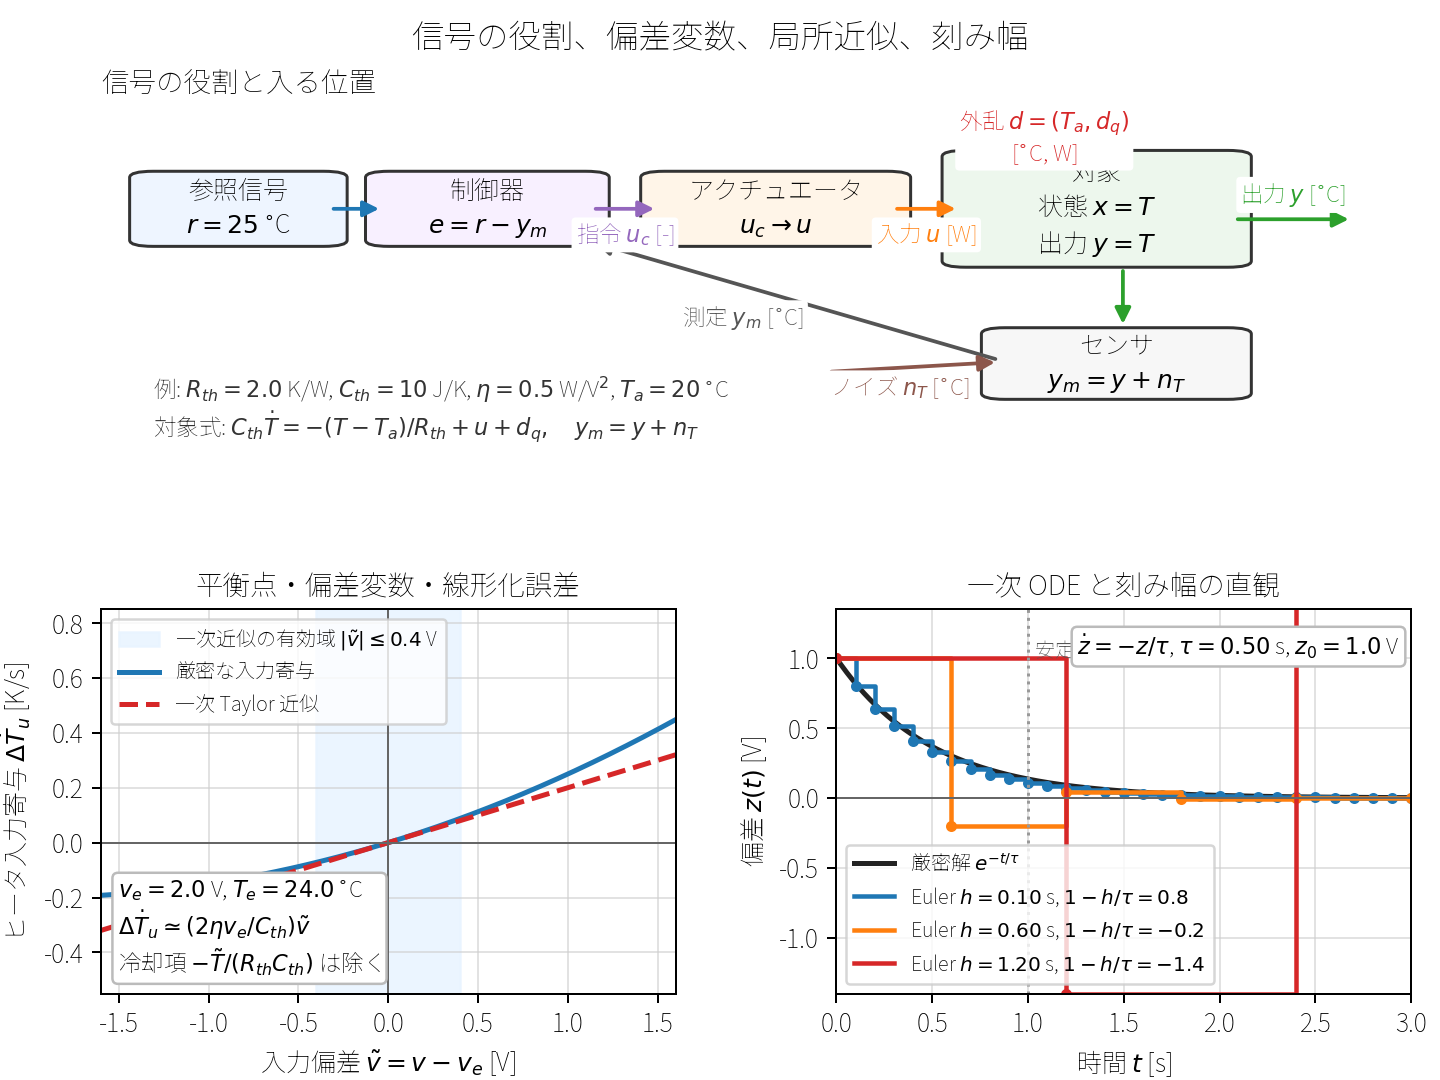
\includegraphics[width=0.96\linewidth,bb=0 0 1440 1080]{figures/signal_modeling_examples.png}
\caption{信号の役割、偏差変数、局所線形化、数値積分刻み幅の対応。上段は熱系における参照信号、入力、出力、外乱、ノイズ、状態の入る位置を示す。左下は $T_a=20\,^\circ\mathrm{C}$、$R_{\mathrm{th}}=2.0\,\mathrm{K/W}$、$C_{\mathrm{th}}=10\,\mathrm{J/K}$、$\eta=0.5\,\mathrm{W/V^2}$、$v_e=2.0\,\mathrm{V}$ の動作点で、ヒータ電圧偏差 $\tilde{v}$ が温度変化率へ与える入力寄与 $\Delta\dot{T}_u$ とその一次 Taylor 近似を比較している。完全な線形化式には、これに加えて冷却による $-\tilde{T}/(R_{\mathrm{th}}C_{\mathrm{th}})$ も入る。右下は $\dot{z}=-z/\tau$、$\tau=0.50\,\mathrm{s}$ に陽的 Euler 法を適用し、刻み幅 $h$ によって精度と数値安定性が変わることを示す。}
\label{fig:signal-modeling-examples}
\end{figure}

\begin{practice}[信号分類と局所近似の確認]
図\ref{fig:signal-modeling-examples} の上段で、対象の状態を直接変える信号と、センサ測定値だけを変える信号をそれぞれ列挙せよ。次に、左下のパラメータから平衡温度 $T_e$ を計算し、$\tilde{v}=0.4\,\mathrm{V}$ と $\tilde{v}=1.2\,\mathrm{V}$ について、温度変化率へのヒータ入力寄与
\begin{equation}
  \frac{\eta\{(v_e+\tilde{v})^2-v_e^2\}}{C_{\mathrm{th}}},
  \qquad
  \frac{2\eta v_e}{C_{\mathrm{th}}}\tilde{v}
\end{equation}
を比較せよ。この二つの量は入力項だけの比較であり、完全な $\dot{\tilde{T}}$ には冷却項 $-\tilde{T}/(R_{\mathrm{th}}C_{\mathrm{th}})$ も加わることを確認せよ。さらに右下の $\tau=0.50\,\mathrm{s}$ について、$h=0.10\,\mathrm{s}$、$0.60\,\mathrm{s}$、$1.20\,\mathrm{s}$ の更新係数 $1-h/\tau$ を求め、連続時間の安定性と数値更新の安定性が一致しない場合を説明せよ。
\end{practice}

\subsubsection{標準例における信号の役割}

熱系では、部屋または小さな物体の代表温度を $T(t)$ [$^\circ\mathrm{C}$] とし、周囲温度を $T_a(t)$ [$^\circ\mathrm{C}$]、ヒータから実際に入る熱流を $u(t)$ [W] とする。熱容量 $C_{\mathrm{th}}$ [J/K] と熱抵抗 $R_{\mathrm{th}}$ [K/W] を一定パラメータとみなすと、単純なモデルは
\begin{equation}
  C_{\mathrm{th}}\dot{T}(t)
  =-\frac{T(t)-T_a(t)}{R_{\mathrm{th}}}+u(t)+d_q(t)
  \label{eq:thermal-signal-example}
\end{equation}
である。状態は $x=T$、入力はヒータ熱流 $u$、外乱は周囲温度 $T_a$ と未知熱流 $d_q$ である。制御したい出力を $y=T$、温度センサの測定値を $y_m=T+n_T$ と置けば、参照信号 $r=T_{\mathrm{ref}}$ は目標温度である。ここで $T_a$ は測れることも測れないこともある。測れる外乱はフィードフォワード補償に使えるが、測れない外乱はフィードバックで結果として抑える。

RC 回路では、コンデンサ電圧を $v_C(t)$ [V]、入力電圧を $u(t)=v_{\mathrm{in}}(t)$ [V]、外からコンデンサ節点へ流れ込む未知電流を $d_i(t)$ [A] とする。抵抗 $R$ [$\Omega$] と容量 $C$ [F] が一定なら、キルヒホッフの電流則から
\begin{equation}
  C\dot{v}_C(t)=\frac{u(t)-v_C(t)}{R}+d_i(t)
  \label{eq:rc-signal-example}
\end{equation}
を得る。$x=v_C$ とすれば、出力は $y=v_C$、センサ測定値は $y_m=v_C+n_v$ である。$R$ や $C$ は信号ではなくパラメータとして扱うが、温度で抵抗値が変わるほど精密に見る場合は、$R(t)$ をゆっくり変化する未知パラメータまたは追加状態として推定することがある。

質量ばねダンパ系では、位置 $q(t)$ [m]、速度 $\dot{q}(t)$ [m/s]、力入力 $u(t)$ [N]、外力外乱 $d_F(t)$ [N] を使う。質量 $M$ [kg]、粘性係数 $c$ [N\,s/m]、ばね定数 $k$ [N/m] を一定とすると、ニュートンの運動方程式は
\begin{equation}
  M\ddot{q}(t)+c\dot{q}(t)+kq(t)=u(t)+d_F(t)
  \label{eq:msd-signal-example}
\end{equation}
である。状態を
\begin{equation}
  x(t)=\begin{bmatrix}q(t)\\ \dot{q}(t)\end{bmatrix}
\end{equation}
と置くと
\begin{align}
  \dot{x}(t)&=
  \begin{bmatrix}
    0&1\\
    -k/M&-c/M
  \end{bmatrix}x(t)
  +\begin{bmatrix}0\\ 1/M\end{bmatrix}u(t)
  +\begin{bmatrix}0\\ 1/M\end{bmatrix}d_F(t),\label{eq:msd-state-signal-example}\\
  y(t)&=\begin{bmatrix}1&0\end{bmatrix}x(t),\\
  y_m(t)&=y(t)+n_q(t)
\end{align}
と書ける。位置センサしかない場合、測定量は位置 $q$ であり、センサ測定値は $q+n_q$ である。速度 $\dot{q}$ は状態の一部だが直接測れていないので、未測定状態である。後でオブザーバや Kalman フィルタを導入するのは、このような未測定状態を、入力と測定値の履歴から推定するためである。

DC モータなら、端子電圧 $v(t)$ [V] は入力、角速度 $\omega(t)$ [rad/s] や角度 $\theta(t)$ [rad] は出力になりうる。負荷トルク $\tau_L(t)$ [N\,m] は、制御器が直接選んでいないので外乱である。電機子インダクタンス $L$ [H]、抵抗 $R$ [$\Omega$]、逆起電力定数 $K_e$ [V\,s/rad]、トルク定数 $K_t$ [N\,m/A]、慣性モーメント $J$ [kg\,m$^2$]、粘性係数 $b$ [N\,m\,s/rad] を一定パラメータとすると、単純化したモデルは
\begin{align}
  L\dot{i}(t)&=-R i(t)-K_e\omega(t)+v(t),\label{eq:dc-motor-current}\\
  J\dot{\omega}(t)&=K_t i(t)-b\omega(t)-\tau_L(t),\label{eq:dc-motor-speed}\\
  \dot{\theta}(t)&=\omega(t).\label{eq:dc-motor-angle}
\end{align}
となる。

DC モータの端子電圧から角度までの関係は、代数的な直接変換ではなく、電気系と機械系の状態を通る因果連鎖として表される。電圧はまず電流を変化させ、電流がトルクを発生させ、トルクが角速度を変化させ、角速度の積分として角度が変化する。この因果連鎖を式の中に残すために、状態を導入する。

DC モータでは
\begin{equation}
  x(t)=\begin{bmatrix}i(t)\\ \omega(t)\\ \theta(t)\end{bmatrix}
\end{equation}
を状態にできる。状態 $x$、入力 $u$、外乱 $d$、パラメータ $p$、出力 $y$ を使うと、多くの対象は
\begin{align}
  \dot{x}(t)&=f(x(t),u(t),d(t),p,t),\label{eq:nonlinear-state-model}\\
  y(t)&=g(x(t),u(t),d(t),p,t)
\end{align}
と書ける。$f$ は内部がどう変わるか、$g$ はどの量が出力として取り出されるかを表す。

状態と出力は同じではない。状態は未来を計算するための内部記述であり、出力は目的やセンサ配置に応じて選ぶ見え方である。DC モータで角度制御をするなら $y=\theta$ と置くことが多いが、電流 $i$ と角速度 $\omega$ も未来の角度を決めるので状態に含める。電流センサがなければ $i$ は未測定状態であり、角度エンコーダがあれば $\theta+n_\theta$ がセンサ測定値である。状態フィードバックの章では $u=-Kx+r_u$ のように状態が使える場合を扱い、推定の章では測定値から $\hat{x}$ を作って、測れない状態を補う。

\subsection{平衡点、偏差変数、線形化}

\begin{definition}[平衡点]
時間に陽に依存しない系 $\dot{x}=f(x,u)$ において、一定入力 $u_e$ と状態 $x_e$ が
\begin{equation}
  f(x_e,u_e)=0
\end{equation}
を満たすとき、$(x_e,u_e)$ を平衡点という。
\end{definition}

平衡点では状態の変化率が 0 なので、入力を $u_e$ に保てば状態は $x_e$ に留まる。熱系なら一定温度、RC 回路なら一定電圧、モータなら一定速度、水槽なら一定水位が平衡点の例である。外乱やパラメータを明示するモデル
\begin{equation}
  \dot{x}=f(x,u,d,p)
\end{equation}
では、一定外乱 $d_e$ とパラメータ $p$ を固定したうえで
\begin{equation}
  f(x_e,u_e,d_e,p)=0
\end{equation}
を満たす組を平衡点として扱う。周囲温度や負荷トルクが変われば、同じ入力でも平衡点は変わりうる。時間に陽に依存するモデルや周期的に動く基準運動では、厳密には一点の平衡点ではなく基準軌道のまわりで偏差を考えるが、本節ではまず一定値に留まる動作点を扱う。

\begin{definition}[偏差変数]
制御では絶対値より平衡点からのずれを見る。そこで
\begin{equation}
  \tilde{x}=x-x_e,
  \qquad
  \tilde{u}=u-u_e
  \label{eq:deviation-definition}
\end{equation}
を偏差変数という。すると $x=x_e+\tilde{x}$、$u=u_e+\tilde{u}$ である。
\end{definition}

偏差変数は無次元の誤差ではない。$x_i$ が温度なら $\tilde{x}_i$ も温度差の単位 K をもち、$u_j$ が力なら $\tilde{u}_j$ も N をもつ。必要なら後で基準値や許容幅で割って無次元化するが、線形化そのものでは物理単位を保ったまま計算する。平衡点は定数なので $\dot{x}_e=0$ であり、
\begin{equation}
  \dot{\tilde{x}}=\frac{\dd}{\dd t}(x-x_e)=\dot{x}
\end{equation}
である。出力も同じ考えで、$y_e=g(x_e,u_e)$ と置けば $\tilde{y}=y-y_e$ を出力偏差として使える。

\begin{definition}[ヤコビアン]
ベクトル値関数 $f(x,u)\in\R^n$ の各成分を各変数で偏微分して並べた行列をヤコビアンという。$x\in\R^n$、$u\in\R^m$ なら
\begin{equation}
  \frac{\pp f}{\pp x}=\left[\frac{\pp f_i}{\pp x_j}\right]_{i,j},
  \qquad
  \frac{\pp f}{\pp u}=\left[\frac{\pp f_i}{\pp u_j}\right]_{i,j}
\end{equation}
である。
\end{definition}

$\dot{x}=f(x,u)$ では $f_i$ の単位は $x_i$/s である。したがって $\pp f_i/\pp x_j$ の単位は $(x_i/\mathrm{s})/x_j$、$\pp f_i/\pp u_j$ の単位は $(x_i/\mathrm{s})/u_j$ になる。$A=\pp f/\pp x$ は $n\times n$ 行列、$B=\pp f/\pp u$ は $n\times m$ 行列であり、$A\tilde{x}$ と $B\tilde{u}$ の各成分はどちらも $x_i$/s の単位をもつ。状態の各成分が位置、速度、電流のように違う単位をもつとき、行列の成分も同じ単位ではない。

\begin{theorem}[一次テイラー展開による線形化]
非線形系 $\dot{x}=f(x,u)$ が平衡点 $(x_e,u_e)$ の近くで十分なめらかなら、偏差変数 $\tilde{x}$、$\tilde{u}$ は一次近似で
\begin{equation}
  \dot{\tilde{x}}=A\tilde{x}+B\tilde{u}
  \label{eq:linearized-model}
\end{equation}
に従う。ただし
\begin{equation}
  A=\left.\frac{\pp f}{\pp x}\right|_{(x_e,u_e)},
  \qquad
  B=\left.\frac{\pp f}{\pp u}\right|_{(x_e,u_e)}
\end{equation}
である。
\end{theorem}

ここで「十分なめらか」とは、少なくとも平衡点の近傍で $f$ の一次偏微分が存在して連続であり、二次の誤差項を小さくできるという意味である。より安全には $f$ が二回連続微分可能で、二階偏微分が近傍で有界であると仮定する。この仮定により、$\delta z=[\tilde{x}^\T,\tilde{u}^\T]^\T$ と置いたとき、捨てた項 $r_2(\delta z)$ は
\begin{equation}
  \lVert r_2(\delta z)\rVert \le c\lVert \delta z\rVert^2
\end{equation}
を満たす定数 $c$ で抑えられる。したがって一次モデルは $\tilde{x}$ と $\tilde{u}$ が小さい範囲でだけ信頼できる。入力飽和、摩擦の符号切替、接触の有無のように式が滑らかでない現象をまたぐと、この線形化の仮定は崩れる。

\begin{derivation}
$x=x_e+\tilde{x}$、$u=u_e+\tilde{u}$ を $\dot{x}=f(x,u)$ に代入する。$x_e$ は定数なので $\dot{x}=\dot{\tilde{x}}$ である。したがって
\begin{equation}
  \dot{\tilde{x}}=f(x_e+\tilde{x},u_e+\tilde{u})
\end{equation}
となる。多変数のテイラー展開を一次まで使うと
\begin{align}
  f(x_e+\tilde{x},u_e+\tilde{u})
  &=f(x_e,u_e)
    +\left.\frac{\pp f}{\pp x}\right|_{(x_e,u_e)}\tilde{x}
    +\left.\frac{\pp f}{\pp u}\right|_{(x_e,u_e)}\tilde{u}
    +\text{二次以上の項}.
\end{align}
平衡点の定義より $f(x_e,u_e)=0$ である。もし選んだ $(x_e,u_e)$ が平衡点でなければ、この定数項が残り、偏差モデルは原点へ留まらない。平衡点近傍だけを見る一次近似では二次以上の項を捨てるので
\begin{equation}
  \dot{\tilde{x}}\simeq A\tilde{x}+B\tilde{u}
\end{equation}
を得る。
\end{derivation}

\begin{example}[熱系の動作点まわりの線形化]
小さな物体の温度 $T(t)$ [K] を、周囲温度 $T_a$ [K] の環境でヒータ電圧 $v(t)$ [V] により調整する。熱容量を $C_{\mathrm{th}}$ [J/K]、熱抵抗を $R_{\mathrm{th}}$ [K/W]、ヒータの電圧二乗係数を $\eta$ [W/V$^2$] とし、ヒータ電力が $\eta v^2$ で近似できるとする。このとき
\begin{equation}
  C_{\mathrm{th}}\dot{T}
  =-\frac{T-T_a}{R_{\mathrm{th}}}+\eta v^2
\end{equation}
である。状態を $x=T$、入力を $u=v$ とすれば
\begin{equation}
  f(T,v)=\frac{1}{C_{\mathrm{th}}}
  \left(-\frac{T-T_a}{R_{\mathrm{th}}}+\eta v^2\right)
\end{equation}
である。一定電圧 $v_e$ で温度が止まる平衡点は
\begin{align}
  0&=-\frac{T_e-T_a}{R_{\mathrm{th}}}+\eta v_e^2,\\
  T_e&=T_a+R_{\mathrm{th}}\eta v_e^2
\end{align}
を満たす。偏差を $\tilde{T}=T-T_e$、$\tilde{v}=v-v_e$ と置くと、
\begin{align}
  \dot{\tilde{T}}
  &=\frac{1}{C_{\mathrm{th}}}
    \left(-\frac{T_e+\tilde{T}-T_a}{R_{\mathrm{th}}}
    +\eta(v_e+\tilde{v})^2\right)\\
  &=\frac{1}{C_{\mathrm{th}}}
    \left(-\frac{T_e-T_a}{R_{\mathrm{th}}}
    -\frac{\tilde{T}}{R_{\mathrm{th}}}
    +\eta v_e^2+2\eta v_e\tilde{v}+\eta\tilde{v}^2\right).
\end{align}
平衡条件により $-(T_e-T_a)/R_{\mathrm{th}}+\eta v_e^2=0$ なので
\begin{equation}
  \dot{\tilde{T}}
  =-\frac{1}{R_{\mathrm{th}}C_{\mathrm{th}}}\tilde{T}
   +\frac{2\eta v_e}{C_{\mathrm{th}}}\tilde{v}
   +\frac{\eta}{C_{\mathrm{th}}}\tilde{v}^2
\end{equation}
となる。一次線形化では最後の二次項を捨てて
\begin{equation}
  \dot{\tilde{T}}
  \simeq
  -\frac{1}{R_{\mathrm{th}}C_{\mathrm{th}}}\tilde{T}
  +\frac{2\eta v_e}{C_{\mathrm{th}}}\tilde{v}
\end{equation}
を得る。ここで
\begin{equation}
  A=-\frac{1}{R_{\mathrm{th}}C_{\mathrm{th}}},
  \qquad
  B=\frac{2\eta v_e}{C_{\mathrm{th}}}
\end{equation}
であり、$A$ の単位は 1/s、$B$ の単位は K/(s\,V) である。$v_e=0$ の動作点では $B=0$ となり、電圧の小さな正負の偏差は一次近似では温度を変えないという式になる。これはヒータ電力を電圧の二乗で近似したためであり、制御入力を電力 $P=\eta v^2$ として選ぶか、実際に使う非零の動作点まわりで線形化する必要がある。
\end{example}

倒立振子で $x=[\theta,\dot{\theta}]^\T$ とし、
\begin{equation}
  f(x,u)=\begin{bmatrix}x_2\\ (mgl\sin x_1+bu)/J\end{bmatrix}
\end{equation}
と書く。直立平衡点 $(x_e,u_e)=(0,0)$ まわりのヤコビアンは
\begin{align}
  A&=\left.\frac{\pp f}{\pp x}\right|_{(0,0)}
   =\begin{bmatrix}
      \pp f_1/\pp x_1 & \pp f_1/\pp x_2\\
      \pp f_2/\pp x_1 & \pp f_2/\pp x_2
    \end{bmatrix}_{(0,0)}\\
   &=\begin{bmatrix}
      0&1\\
      (mgl/J)\cos x_1&0
    \end{bmatrix}_{x_1=0}
    =\begin{bmatrix}0&1\\ mgl/J&0\end{bmatrix},\\
  B&=\left.\frac{\pp f}{\pp u}\right|_{(0,0)}
   =\begin{bmatrix}0\\ b/J\end{bmatrix}.
\end{align}
この計算で、$\sin\theta\simeq\theta$ という近似を単独の経験則として使ったのではない。ヤコビアンを計算した結果として、直立近傍の一次モデルが得られている。

\subsection{物理法則から状態方程式を構成する手順}

状態方程式は、物理法則を行列記法へ置き換えただけのものではない。保存される量、流れとして入る量、素子や機構の構成則、入力と出力の選び方を順に固定し、将来の変化を一階微分方程式として計算できる形に整理したものである。集中定数モデルで最初に作る形は
\begin{align}
  \dot{x}(t)&=f(x(t),u(t),d(t),p,t),\\
  y(t)&=g(x(t),u(t),d(t),p,t)
\end{align}
である。線形時不変に近似できる場合は
\begin{align}
  \dot{x}(t)&=Ax(t)+Bu(t)+Ed(t),\label{eq:physical-modeling-state-form}\\
  y(t)&=C_y x(t)+D_y u(t)+F_y d(t)
\end{align}
と書く。ここで $C_y$ は出力行列であり、電気容量を表す $C$ と混同しないように添字を付けている。

\begin{definition}[構成則]
保存則や運動方程式だけでは、流れ、力、電圧、温度差の関係は決まらない。熱流と温度差、電流と電圧差、ばね力と変位、粘性力と速度のように、対象を構成する要素ごとの関係式を構成則という。
\end{definition}

物理モデルを状態方程式にする手順は、次の形にそろえられる。

\begin{enumerate}
  \item 蓄積される量を決める。熱なら内部エネルギー、電気なら電荷、機械なら運動量とばねの変位に相当する量である。
  \item 保存則または運動方程式を書く。蓄積量の時間変化率は、流入、流出、生成、外乱の和で決まる。
  \item 構成則で未知の流れや力を状態、入力、外乱、パラメータで表す。
  \item 入力 $u$、外乱 $d$、出力 $y$ を単位つきで選ぶ。
  \item 将来計算に必要な最小限の量を状態 $x$ とし、すべてを $\dot{x}=f(x,u,d,p,t)$ の形へ解く。二階微分が出る場合は、速度を新しい状態にして一階の連立方程式へ直す。
\end{enumerate}

この手順では、状態を「測れる量」として選ぶのではなく、「以後の変化を計算するのに必要な量」として選ぶ。測れる量は出力 $y$ に置く。状態を選んだ後で出力方程式を作ると、測定できる量と内部に保持すべき量を分けられる。

図\ref{fig:physical-modeling-examples} は、以後の導出で使う標準例を、蓄積要素、入力、外乱、出力の位置として並べたものである。熱系と RC 回路は一つの蓄積要素から一次モデルになり、質量ばねダンパ系と DC モータは速度、電流、角速度のような内部量を状態として残すことで一階の連立方程式になる。図の矢印は信号の向きだけでなく、式の右辺で正負どちらに入るかを確認するための手掛かりでもある。

\begin{figure}[tb]
\centering
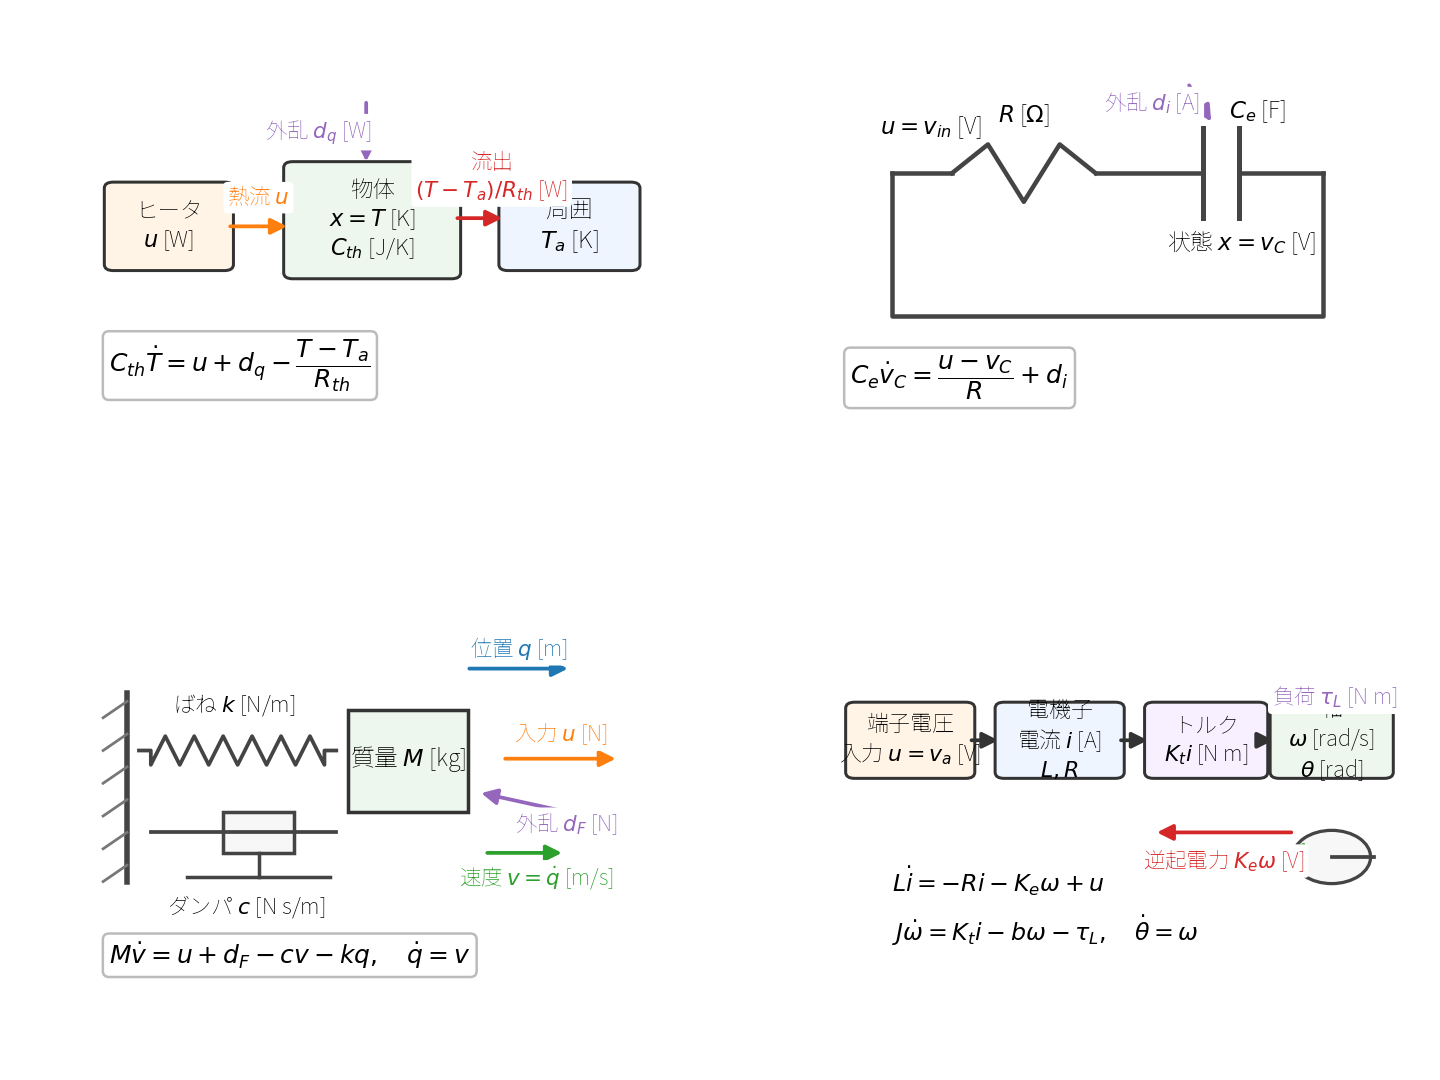
\includegraphics[width=0.96\linewidth,bb=0 0 1440 1080]{figures/physical_modeling_examples.png}
\caption{物理法則から状態方程式へ進む標準例。熱収支では内部エネルギーの蓄積、RC 回路では電荷の蓄積、質量ばねダンパ系では位置と速度、DC モータでは電流、角速度、角度を状態として残す。各パネルは入力、外乱、代表パラメータ、状態の単位を対応させ、保存則または運動方程式から $\dot{x}=f(x,u,d,p)$ へ整理する起点を示している。}
\label{fig:physical-modeling-examples}
\end{figure}

\begin{practice}[物理モデルの構造分類]
図\ref{fig:physical-modeling-examples} の四つの例について、蓄積される量、状態、入力、外乱、出力候補を一つずつ表にせよ。次に、熱系と RC 回路の式を見比べ、$C_{\mathrm{th}}$ と $C_e$、$R_{\mathrm{th}}$ と $R$、$T$ と $v_C$ がそれぞれどの役割に対応するかを説明せよ。最後に、質量ばねダンパ系で位置 $q$ だけを状態にした場合に未来の計算で不足する量を答えよ。
\end{practice}

\subsubsection{熱系の収支式からの導出}

一つの代表温度で表せる小さな物体を考える。温度を $T(t)$ [K]、周囲温度を $T_a(t)$ [K]、ヒータ熱流を $u(t)$ [W]、未知の熱流外乱を $d_q(t)$ [W] とする。熱容量を $C_{\mathrm{th}}$ [J/K]、熱抵抗を $R_{\mathrm{th}}$ [K/W] とし、物体内部の温度分布は無視できると仮定する。

蓄積される量は内部エネルギーであり、基準エネルギーを除けば変化率は
\begin{equation}
  \dot{E}(t)=C_{\mathrm{th}}\dot{T}(t)
\end{equation}
と書ける。単位は $(\mathrm{J/K})(\mathrm{K/s})=\mathrm{J/s}=\mathrm{W}$ であり、熱流と一致する。熱抵抗の構成則により、物体から周囲へ出る熱流は
\begin{equation}
  q_{\mathrm{out}}(t)=\frac{T(t)-T_a(t)}{R_{\mathrm{th}}}
\end{equation}
である。したがって熱収支は
\begin{align}
  C_{\mathrm{th}}\dot{T}(t)
  &=u(t)+d_q(t)-q_{\mathrm{out}}(t)\\
  &=u(t)+d_q(t)-\frac{T(t)-T_a(t)}{R_{\mathrm{th}}}
\end{align}
となる。状態を $x=T$、入力を $u$、外乱を
\begin{equation}
  d(t)=\begin{bmatrix}T_a(t)\\ d_q(t)\end{bmatrix}
\end{equation}
と選ぶと、一階の状態方程式は
\begin{equation}
  \dot{x}(t)
  =-\frac{1}{R_{\mathrm{th}}C_{\mathrm{th}}}x(t)
   +\frac{1}{C_{\mathrm{th}}}u(t)
   +\begin{bmatrix}
      \dfrac{1}{R_{\mathrm{th}}C_{\mathrm{th}}}&
      \dfrac{1}{C_{\mathrm{th}}}
    \end{bmatrix}d(t)
\end{equation}
である。出力として温度を測るなら
\begin{equation}
  y(t)=x(t)
\end{equation}
でよい。行列表示では $A=-1/(R_{\mathrm{th}}C_{\mathrm{th}})$、$B=1/C_{\mathrm{th}}$ であり、$A$ の単位は 1/s、$B$ の単位は K/J である。$B u$ の単位は $(\mathrm{K/J})(\mathrm{J/s})=\mathrm{K/s}$ となり、$\dot{x}$ の単位と一致する。

\subsubsection{RC 回路のキルヒホッフ則からの導出}

抵抗とコンデンサからなる一次の RC 回路を考える。入力電圧を $u(t)=v_{\mathrm{in}}(t)$ [V]、コンデンサ電圧を $v_C(t)$ [V]、節点へ流れ込む未知電流を $d_i(t)$ [A] とする。抵抗を $R$ [$\Omega$]、容量を $C_e$ [F] とし、抵抗と容量は一定、配線の寄生成分は無視できると仮定する。

蓄積される量はコンデンサの電荷
\begin{equation}
  Q_C(t)=C_e v_C(t)
\end{equation}
である。電荷の時間変化率は電流なので
\begin{equation}
  \dot{Q}_C(t)=C_e\dot{v}_C(t)
\end{equation}
であり、単位は $\mathrm{C/s}=\mathrm{A}$ である。抵抗を流れてコンデンサ節点へ入る電流は、オームの法則により
\begin{equation}
  i_R(t)=\frac{u(t)-v_C(t)}{R}
\end{equation}
である。キルヒホッフの電流則を節点に適用すると、コンデンサへ流れ込む電流の和が電荷の増加率になるため
\begin{align}
  C_e\dot{v}_C(t)&=i_R(t)+d_i(t)\\
  &=\frac{u(t)-v_C(t)}{R}+d_i(t)
\end{align}
を得る。状態を $x=v_C$、入力を $u=v_{\mathrm{in}}$、外乱を $d=d_i$ と置けば
\begin{align}
  \dot{x}(t)&=-\frac{1}{RC_e}x(t)+\frac{1}{RC_e}u(t)+\frac{1}{C_e}d(t),\\
  y(t)&=x(t)
\end{align}
である。このモデルでは $A=-1/(RC_e)$、$B=1/(RC_e)$ であり、どちらも 1/s の単位をもつ。電流外乱の係数 $1/C_e$ は、電流 [A] を電圧変化率 [V/s] に変える係数である。熱系と RC 回路の式が同じ形になるのは、熱容量とコンデンサ容量が蓄積を表し、熱抵抗と電気抵抗が差に比例する流れを作るからである。

\subsubsection{質量ばねダンパ系の運動方程式からの導出}

水平直線上の質量を考える。位置を $q(t)$ [m]、速度を $v(t)=\dot{q}(t)$ [m/s]、入力として加える力を $u(t)$ [N]、外力外乱を $d_F(t)$ [N] とする。質量を $M$ [kg]、粘性係数を $c$ [N\,s/m]、ばね定数を $k$ [N/m] とし、ばねの自然長からの変位を $q=0$ 基準で測る。

機械系では、力のつり合いではなくニュートンの第二法則を使う。運動量 $Mv$ の時間変化率が力の和であるから
\begin{equation}
  M\dot{v}(t)=\sum F(t)
\end{equation}
である。ばね力と粘性力の構成則を
\begin{equation}
  F_k(t)=-kq(t),\qquad F_c(t)=-cv(t)
\end{equation}
と置くと
\begin{align}
  M\dot{v}(t)&=u(t)+d_F(t)-cv(t)-kq(t),\\
  \dot{q}(t)&=v(t)
\end{align}
を得る。二階微分方程式としては
\begin{equation}
  M\ddot{q}(t)+c\dot{q}(t)+kq(t)=u(t)+d_F(t)
\end{equation}
であるが、状態方程式では一階の連立方程式に直す。状態を
\begin{equation}
  x(t)=\begin{bmatrix}q(t)\\ v(t)\end{bmatrix}
\end{equation}
と選ぶと
\begin{align}
  \dot{x}(t)
  &=\begin{bmatrix}
      0&1\\
      -k/M&-c/M
    \end{bmatrix}x(t)
    +\begin{bmatrix}
      0\\
      1/M
    \end{bmatrix}u(t)
    +\begin{bmatrix}
      0\\
      1/M
    \end{bmatrix}d_F(t),\label{eq:physical-modeling-msd-state}\\
  y(t)&=\begin{bmatrix}1&0\end{bmatrix}x(t)
\end{align}
となる。位置だけを測る場合は出力行列が $\begin{bmatrix}1&0\end{bmatrix}$ であり、速度まで測る場合は $y=x$ としてよい。\weq{physical-modeling-msd-state} の $A_{21}=-k/M$ は 1/s$^2$、$A_{22}=-c/M$ は 1/s、$B_2=1/M$ は 1/kg の単位をもつ。状態の成分 $q$ と $v$ の単位が異なるため、状態行列の各成分の単位も異なる。

熱系と RC 回路では一つの蓄積要素から一つの状態が生じた。質量ばねダンパ系では、位置だけでは次の位置を計算できず、速度も必要になる。したがって状態は $q$ だけでなく $v$ を含む。この違いは、モデルの次数が「式の見た目」ではなく、蓄積要素と将来計算に必要な情報の数で決まることを示している。

\subsubsection{DC モータの電気機械結合モデルの導出}

直流モータは、電気回路と回転運動が結合した標準的な制御対象である。ここでは電機子制御の DC モータを考え、端子電圧を $u(t)=v_a(t)$ [V]、電機子電流を $i(t)$ [A]、回転角を $\theta(t)$ [rad]、角速度を $\omega(t)=\dot{\theta}(t)$ [rad/s]、負荷トルクを $\tau_L(t)$ [N\,m] とする。電機子インダクタンスを $L$ [H]、電機子抵抗を $R$ [$\Omega$]、逆起電力定数を $K_e$ [V\,s/rad]、トルク定数を $K_t$ [N\,m/A]、回転部の等価慣性モーメントを $J$ [kg\,m$^2$]、粘性摩擦係数を $b$ [N\,m\,s/rad] とする。磁束は一定、磁気飽和、ブラシ電圧降下、クーロン摩擦、軸のねじれは無視し、すべてのパラメータは一定と仮定する。

電気側ではキルヒホッフの電圧則を使う。電機子端子に加えた電圧は、インダクタンスの電圧降下、抵抗の電圧降下、回転によって生じる逆起電力の和である。構成則を
\begin{equation}
  v_L(t)=L\dot{i}(t),\qquad
  v_R(t)=Ri(t),\qquad
  e_b(t)=K_e\omega(t)
\end{equation}
と置くと
\begin{equation}
  u(t)=L\dot{i}(t)+Ri(t)+K_e\omega(t)
\end{equation}
である。したがって電流の状態方程式は
\begin{equation}
  \dot{i}(t)=-\frac{R}{L}i(t)-\frac{K_e}{L}\omega(t)+\frac{1}{L}u(t)
  \label{eq:dcmotor-current-state}
\end{equation}
となる。各項の単位は A/s でそろう。たとえば $R i/L$ は V/H であり、$1\,\mathrm{H}=1\,\mathrm{V\,s/A}$ だから A/s である。

機械側では、回転に関するニュートンの第二法則を使う。角運動量 $J\omega$ の時間変化率は、軸まわりのトルクの和である。モータが作るトルクと粘性摩擦トルクを
\begin{equation}
  \tau_m(t)=K_t i(t),\qquad
  \tau_b(t)=b\omega(t)
\end{equation}
と置けば
\begin{equation}
  J\dot{\omega}(t)=K_t i(t)-b\omega(t)-\tau_L(t)
\end{equation}
であり、
\begin{equation}
  \dot{\omega}(t)=\frac{K_t}{J}i(t)-\frac{b}{J}\omega(t)-\frac{1}{J}\tau_L(t)
  \label{eq:dcmotor-speed-state}
\end{equation}
を得る。さらに角度は角速度の積分で決まるため
\begin{equation}
  \dot{\theta}(t)=\omega(t)
  \label{eq:dcmotor-angle-state}
\end{equation}
である。

角度制御まで含めるなら、状態を
\begin{equation}
  x(t)=\begin{bmatrix}i(t)\\ \omega(t)\\ \theta(t)\end{bmatrix},
  \qquad d(t)=\tau_L(t)
\end{equation}
と選ぶ。\weq{dcmotor-current-state}--\weq{dcmotor-angle-state} をまとめると
\begin{align}
  \dot{x}(t)
  &=
  \begin{bmatrix}
    -R/L&-K_e/L&0\\
    K_t/J&-b/J&0\\
    0&1&0
  \end{bmatrix}x(t)
  +\begin{bmatrix}
    1/L\\
    0\\
    0
  \end{bmatrix}u(t)
  +\begin{bmatrix}
    0\\
    -1/J\\
    0
  \end{bmatrix}d(t),\label{eq:dcmotor-state-space}\\
  y(t)&=C_y x(t)+D_y u(t)
\end{align}
となる。角速度を測って速度制御をする場合は $C_y=\begin{bmatrix}0&1&0\end{bmatrix}$、$D_y=0$ と置く。角度エンコーダで位置制御をする場合は $C_y=\begin{bmatrix}0&0&1\end{bmatrix}$ である。電流センサとエンコーダの両方を使うなら
\begin{equation}
  y(t)=
  \begin{bmatrix}
    1&0&0\\
    0&0&1
  \end{bmatrix}x(t)
\end{equation}
のように出力を複数にしてよい。

パラメータの意味は、応答の速さと結合の強さに直接現れる。$L/R$ は電気的時定数であり、回転が止まっていて逆起電力がないときの電流の立ち上がりを決める。$J/b$ は、電流を 0 として粘性摩擦だけで減速するときの機械的時定数である。$K_e$ が大きいほど同じ角速度で大きな逆起電力が生じ、電流の増加を抑える。$K_t$ が大きいほど同じ電流で大きなトルクが得られる。SI 単位系で同じ物理変換を理想的に表すと $K_t$ と $K_e$ の数値は一致するが、制御モデルでは単位と符号の定義を明示してから使う必要がある。負荷トルク $\tau_L$ は入力電圧で直接選べないため外乱として置き、速度低下や位置誤差を通じて観測される。

速度制御だけが目的で、角度 $\theta$ が出力にも制約にも入らない場合は、状態を $x=[i,\omega]^\T$ に縮約できる。一方、電気的時定数 $L/R$ が制御周期や機械応答に比べて十分小さい場合は、近似的に $L\dot{i}\simeq0$ と置き
\begin{equation}
  i(t)\simeq\frac{u(t)-K_e\omega(t)}{R}
\end{equation}
として、電流状態を消去する低次モデルを作ることもある。この近似は電流制御器が内側で十分速く働く場合にも使われる。ただし電流制限や過渡的なトルク応答を評価する設計では、\weq{dcmotor-state-space} のように電流を状態として残す方が適切である。

熱、電気、並進機械、回転機械の四例だけでは、保存則が流量で決まる対象と、重力で非線形な復元力を受ける対象をまだ十分に分けられない。水位制御では、センサが水位を測り、ポンプや弁が流量を変える。振子では、角度を測り、支点トルクで姿勢を変える。どちらも低次の制御対象として扱えるが、タンクでは流出量が水位の平方根に依存し、振子では重力項が $\sin\theta$ に依存する。図\ref{fig:tank-pendulum-modeling-examples} は、この二つの対象で、蓄積量、構成則、局所近似、パラメータ変化を対応させたものである。

\begin{figure}[tb]
\centering
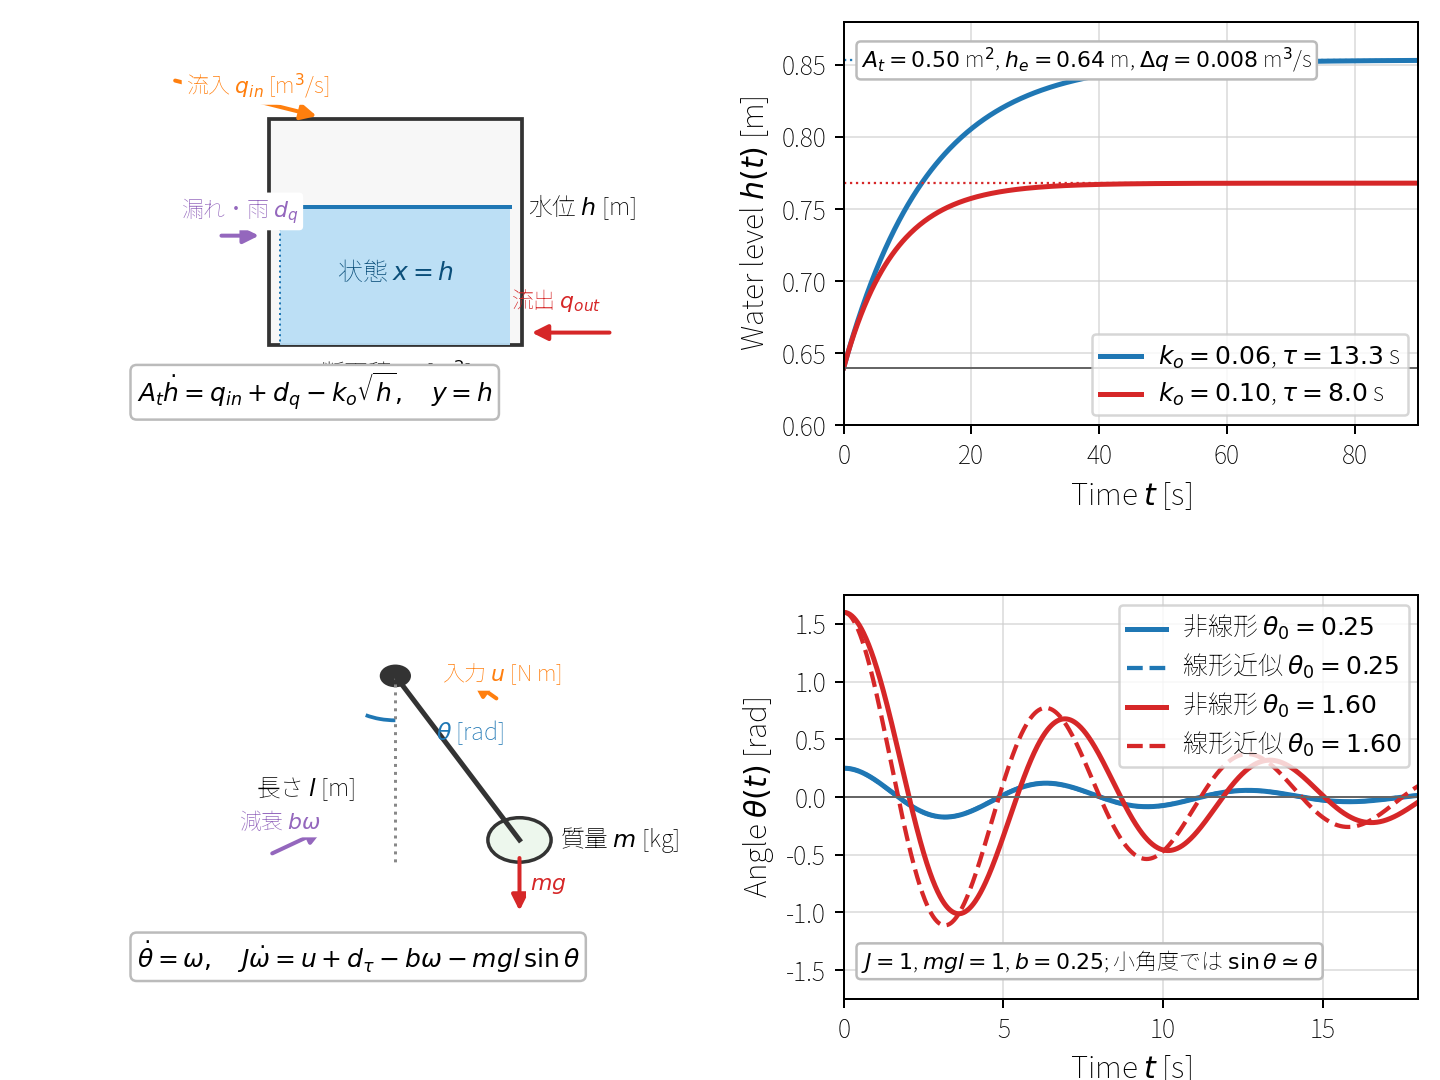
\includegraphics[width=0.96\linewidth,bb=0 0 1440 1080]{figures/tank_pendulum_modeling_examples.png}
\caption{タンク水位モデルと単振子モデルの構造。タンクでは体積保存則と流出構成則から水位の状態方程式が得られ、流出係数 $k_o$ を変えると線形化後の時定数と定常水位変化が同時に変わる。単振子ではトルク、重力、粘性減衰から角度と角速度の状態方程式が得られ、小角度では線形近似と非線形応答が一致しやすいが、大振幅では周期と振幅がずれる。}
\label{fig:tank-pendulum-modeling-examples}
\end{figure}

\subsubsection{単一タンクの水位状態方程式}

断面積が一定のタンクを考える。水位を $h(t)$ [m]、断面積を $A_t$ [m$^2$]、ポンプ流入を $q_{\mathrm{in}}(t)$ [m$^3$/s]、雨や漏れをまとめた流量外乱を $d_q(t)$ [m$^3$/s] とする。出力は水位センサで測る $y(t)=h(t)$ とする。タンク内の水量は体積
\begin{equation}
  V(t)=A_t h(t)
\end{equation}
であり、体積の時間変化率は流入から流出を引いた正味流量で決まる。

底の小さな出口から大気中へ流れる場合、流速は水位差によって変わる。ここでは出口断面積、流量係数、重力加速度をまとめた係数 $k_o$ を用いて
\begin{equation}
  q_{\mathrm{out}}(t)=k_o\sqrt{h(t)},\qquad h(t)\ge0
\end{equation}
と書く。$q_{\mathrm{out}}$ の単位は m$^3$/s なので、$k_o$ の単位は m$^{5/2}$/s である。したがって保存則は
\begin{align}
  \frac{\dd}{\dd t}\{A_t h(t)\}
  &=q_{\mathrm{in}}(t)+d_q(t)-q_{\mathrm{out}}(t)\\
  A_t\dot{h}(t)
  &=q_{\mathrm{in}}(t)+d_q(t)-k_o\sqrt{h(t)}
\end{align}
となる。状態を $x=h$ と選べば、非線形状態方程式は
\begin{align}
  \dot{x}(t)&=\frac{1}{A_t}\{q_{\mathrm{in}}(t)+d_q(t)-k_o\sqrt{x(t)}\},\label{eq:tank-level-state}\\
  y(t)&=x(t)
\end{align}
である。

一定流入 $q_{\mathrm{in},e}$ と一定外乱 $d_{q,e}$ のもとで水位 $h_e>0$ が保たれるには
\begin{equation}
  q_{\mathrm{in},e}+d_{q,e}=k_o\sqrt{h_e}
  \label{eq:tank-level-equilibrium}
\end{equation}
が必要である。この平衡点の近くで
\begin{equation}
  \tilde{h}=h-h_e,\qquad
  \tilde{q}_{\mathrm{in}}=q_{\mathrm{in}}-q_{\mathrm{in},e},\qquad
  \tilde{d}_q=d_q-d_{q,e}
\end{equation}
と置く。平方根を一次 Taylor 展開すると
\begin{equation}
  \sqrt{h_e+\tilde{h}}
  =\sqrt{h_e}+\frac{1}{2\sqrt{h_e}}\tilde{h}
  +O(\tilde{h}^2)
\end{equation}
である。\weq{tank-level-equilibrium} を使って定数項を消すと、一次近似は
\begin{equation}
  A_t\dot{\tilde{h}}
  =\tilde{q}_{\mathrm{in}}+\tilde{d}_q
  -\frac{k_o}{2\sqrt{h_e}}\tilde{h}
\end{equation}
となる。したがって
\begin{equation}
  \dot{\tilde{h}}
  =-\frac{k_o}{2A_t\sqrt{h_e}}\tilde{h}
   +\frac{1}{A_t}\tilde{q}_{\mathrm{in}}
   +\frac{1}{A_t}\tilde{d}_q
  \label{eq:tank-level-linearization}
\end{equation}
である。流出係数 $k_o$ が大きいほど、水位のずれを戻す係数 $k_o/(2A_t\sqrt{h_e})$ は大きくなり、時定数
\begin{equation}
  \tau_h=\frac{2A_t\sqrt{h_e}}{k_o}
\end{equation}
は短くなる。一方、同じ流入増分 $\Delta q$ に対する定常水位増分は
\begin{equation}
  \Delta h_\infty=\frac{2\sqrt{h_e}}{k_o}\Delta q
\end{equation}
であり、$k_o$ が大きいほど小さい。図\ref{fig:tank-pendulum-modeling-examples} の右上は、この二つの効果を同じ線形化モデルで示している。

\subsubsection{単振子のトルク入力状態方程式}

長さ $l$ [m] の軽い棒の先に質量 $m$ [kg] があり、支点まわりにトルク入力 $u(t)$ [N\,m] を加えられる単振子を考える。角度 $\theta(t)$ [rad] は下向きから測り、角速度を $\omega(t)=\dot{\theta}(t)$ [rad/s] とする。支点の粘性減衰係数を $b$ [N\,m\,s/rad]、外乱トルクを $d_\tau(t)$ [N\,m] とし、棒の質量と支点の摩擦以外の損失は無視する。質点モデルでは支点まわりの慣性モーメントは
\begin{equation}
  J=ml^2
\end{equation}
である。

角運動量 $J\omega$ の時間変化率は、支点まわりのトルクの和で決まる。入力トルクと外乱トルクは正方向へ入り、粘性減衰は $-b\omega$、重力の復元トルクは $-mgl\sin\theta$ である。したがって
\begin{equation}
  J\dot{\omega}(t)
  =u(t)+d_\tau(t)-b\omega(t)-mgl\sin\theta(t)
\end{equation}
であり、状態を
\begin{equation}
  x(t)=\begin{bmatrix}\theta(t)\\ \omega(t)\end{bmatrix}
\end{equation}
と置くと
\begin{align}
  \dot{x}_1(t)&=x_2(t),\\
  \dot{x}_2(t)&=\frac{1}{J}\{u(t)+d_\tau(t)-b x_2(t)-mgl\sin x_1(t)\},\label{eq:pendulum-state}\\
  y(t)&=x_1(t)
\end{align}
を得る。

角度 $\theta_e$ で静止させたいとき、$\omega_e=0$ として平衡入力は
\begin{equation}
  u_e=mgl\sin\theta_e-d_{\tau,e}
\end{equation}
である。偏差を $\tilde{\theta}=\theta-\theta_e$、$\tilde{\omega}=\omega$、$\tilde{u}=u-u_e$、$\tilde{d}_\tau=d_\tau-d_{\tau,e}$ と置き、$\sin(\theta_e+\tilde{\theta})$ を一次 Taylor 展開すると
\begin{equation}
  \sin(\theta_e+\tilde{\theta})
  =\sin\theta_e+\cos\theta_e\,\tilde{\theta}+O(\tilde{\theta}^2)
\end{equation}
である。定数項は平衡条件で消えるので、接線モデルは
\begin{equation}
  \begin{bmatrix}
    \dot{\tilde{\theta}}\\
    \dot{\tilde{\omega}}
  \end{bmatrix}
  =
  \begin{bmatrix}
    0&1\\
    -mgl\cos\theta_e/J&-b/J
  \end{bmatrix}
  \begin{bmatrix}
    \tilde{\theta}\\
    \tilde{\omega}
  \end{bmatrix}
  +\begin{bmatrix}0\\1/J\end{bmatrix}\tilde{u}
  +\begin{bmatrix}0\\1/J\end{bmatrix}\tilde{d}_\tau .
  \label{eq:pendulum-linearization}
\end{equation}
下向き平衡点 $\theta_e=0$ では $\cos\theta_e=1$ なので重力項は復元力として働く。上向き平衡点 $\theta_e=\pi$ では $\cos\theta_e=-1$ なので符号が反転し、角度のずれをさらに大きくする不安定化項になる。同じ振子でも、平衡点をどこに選ぶかにより線形化モデルの安定性が変わる。

図\ref{fig:tank-pendulum-modeling-examples} の右下では、$J=1$、$mgl=1$、$b=0.25$ として下向き平衡点まわりの自由応答を比べている。初期角度が $0.25\,\mathrm{rad}$ 程度なら $\sin\theta\simeq\theta$ による線形近似は非線形応答とよく合う。一方、初期角度が $1.60\,\mathrm{rad}$ まで大きくなると、復元トルクが角度に比例しなくなり、振動周期と振幅の減衰が線形近似からずれる。この差は、線形化が「対象を単純にする公式」ではなく、平衡点近くの局所モデルであることを示している。

\begin{practice}[タンクと単振子の状態選択]
図\ref{fig:tank-pendulum-modeling-examples} のタンクについて、$A_t=0.50\,\mathrm{m^2}$、$h_e=0.64\,\mathrm{m}$、$k_o=0.10\,\mathrm{m^{5/2}/s}$ のとき、外乱が 0 なら平衡流入 $q_{\mathrm{in},e}$ はいくらか計算せよ。次に \weq{tank-level-linearization} の係数 $k_o/(2A_t\sqrt{h_e})$ と時定数 $\tau_h$ を求め、$k_o=0.06\,\mathrm{m^{5/2}/s}$ の場合と比べよ。単振子については、\weq{pendulum-linearization} で $\theta_e=0$ と $\theta_e=\pi$ を代入し、重力項の符号が変わる理由を、下向き平衡点と上向き平衡点の小さなずれに対応させて説明せよ。
\end{practice}

\subsubsection{台車上倒立振子の非線形モデルと線形化}

倒立振子は、非線形性、不安定平衡点、状態選択、線形化の意味を同時に示す標準例である。ここでは水平に動く台車の上に剛体棒を取り付けた系を、棒の重心に質量が集中したモデルとして導く。台車位置を $q(t)$ [m]、台車速度を $v(t)=\dot{q}(t)$ [m/s]、振子角を $\theta(t)$ [rad]、角速度を $\omega(t)=\dot{\theta}(t)$ [rad/s] とする。角度 $\theta=0$ は直立上向きであり、$\theta>0$ は重心が右へ傾く向きとする。台車質量を $M$ [kg]、振子質量を $m$ [kg]、支点から重心までの距離を $l$ [m]、重力加速度を $g$ [m/s$^2$]、台車へ加える水平力を $u(t)$ [N] とする。車輪や支点の摩擦、棒の慣性、アクチュエータの飽和はまず無視する。

振子重心の座標を、上向きを正の鉛直方向として
\begin{equation}
  X(t)=q(t)+l\sin\theta(t),\qquad
  Y(t)=l\cos\theta(t)
\end{equation}
と書く。速度は
\begin{equation}
  \dot{X}=\dot{q}+l\cos\theta\,\dot{\theta},
  \qquad
  \dot{Y}=-l\sin\theta\,\dot{\theta}
\end{equation}
である。運動エネルギー $T$ と位置エネルギー $V$ は
\begin{align}
  T&=\frac{1}{2}M\dot{q}^2
    +\frac{1}{2}m(\dot{X}^2+\dot{Y}^2)\\
   &=\frac{1}{2}(M+m)\dot{q}^2
    +m l\cos\theta\,\dot{q}\dot{\theta}
    +\frac{1}{2}m l^2\dot{\theta}^2,\\
  V&=m g l\cos\theta
\end{align}
である。一般化座標を $q$ と $\theta$ とし、ラグランジアンを $\mathcal{L}=T-V$ とする。台車方向の一般化力は $Q_q=u$、角度方向の一般化力は $Q_\theta=0$ である。

オイラー・ラグランジュ方程式
\begin{equation}
  \frac{\dd}{\dd t}\frac{\pp \mathcal{L}}{\pp \dot{q}_j}
  -\frac{\pp \mathcal{L}}{\pp q_j}=Q_j
\end{equation}
を $q$ に適用する。まず
\begin{equation}
  \frac{\pp \mathcal{L}}{\pp \dot{q}}
  =(M+m)\dot{q}+m l\cos\theta\,\dot{\theta}
\end{equation}
であり、
\begin{equation}
  \frac{\dd}{\dd t}\frac{\pp \mathcal{L}}{\pp \dot{q}}
  =(M+m)\ddot{q}+m l\cos\theta\,\ddot{\theta}
  -m l\sin\theta\,\dot{\theta}^2
\end{equation}
となる。$\mathcal{L}$ は $q$ に陽に依存しないので $\pp\mathcal{L}/\pp q=0$ である。したがって
\begin{equation}
  (M+m)\ddot{q}+m l\cos\theta\,\ddot{\theta}
  -m l\sin\theta\,\dot{\theta}^2=u
  \label{eq:cartpole-q-equation}
\end{equation}
を得る。

同じ式を $\theta$ に適用する。偏微分は
\begin{align}
  \frac{\pp \mathcal{L}}{\pp \dot{\theta}}
  &=m l\cos\theta\,\dot{q}+m l^2\dot{\theta},\\
  \frac{\dd}{\dd t}\frac{\pp \mathcal{L}}{\pp \dot{\theta}}
  &=m l\cos\theta\,\ddot{q}
    -m l\sin\theta\,\dot{\theta}\dot{q}
    +m l^2\ddot{\theta},\\
  \frac{\pp \mathcal{L}}{\pp \theta}
  &=-m l\sin\theta\,\dot{q}\dot{\theta}
    +m g l\sin\theta
\end{align}
である。これを差し引くと速度積の項が消え、
\begin{equation}
  m l\cos\theta\,\ddot{q}+m l^2\ddot{\theta}
  -m g l\sin\theta=0
  \label{eq:cartpole-theta-equation}
\end{equation}
となる。\weq{cartpole-q-equation} と \weq{cartpole-theta-equation} を加速度についてまとめると
\begin{equation}
  \begin{bmatrix}
    M+m&m l\cos\theta\\
    m l\cos\theta&m l^2
  \end{bmatrix}
  \begin{bmatrix}
    \ddot{q}\\
    \ddot{\theta}
  \end{bmatrix}
  =
  \begin{bmatrix}
    u+m l\sin\theta\,\dot{\theta}^2\\
    m g l\sin\theta
  \end{bmatrix}.
  \label{eq:cartpole-mass-matrix}
\end{equation}
左辺の行列は、一般化座標に対応する慣性行列である。行列式は
\begin{equation}
  \Delta(\theta)=m l^2\{M+m\sin^2\theta\}
\end{equation}
であり、$M>0$、$m>0$、$l>0$ なら常に正である。したがって加速度を一意に解ける。

状態を
\begin{equation}
  x(t)=\begin{bmatrix}q(t)\\ v(t)\\ \theta(t)\\ \omega(t)\end{bmatrix}
\end{equation}
と置き、$v=\dot{q}$、$\omega=\dot{\theta}$ を使うと、非線形状態方程式は
\begin{align}
  \dot{x}_1&=x_2,\\
  \dot{x}_2&=
  \frac{u+m l x_4^2\sin x_3-m g\sin x_3\cos x_3}
       {M+m\sin^2 x_3},\label{eq:cartpole-nonlinear-qddot}\\
  \dot{x}_3&=x_4,\\
  \dot{x}_4&=
  \frac{(M+m)g\sin x_3-\cos x_3\{u+m l x_4^2\sin x_3\}}
       {l\{M+m\sin^2 x_3\}}.
  \label{eq:cartpole-nonlinear-thetaddot}
\end{align}
台車位置と振子角を測るなら、出力方程式は
\begin{equation}
  y(t)=
  \begin{bmatrix}
    1&0&0&0\\
    0&0&1&0
  \end{bmatrix}x(t)
\end{equation}
である。速度センサがない場合でも $v$ と $\omega$ は未来を決めるために状態に含める。測定されない速度は、数値微分、オブザーバ、または推定器で補う対象になる。

直立平衡点は、任意の一定位置 $q_e$ に対して
\begin{equation}
  x_e=\begin{bmatrix}q_e\\ 0\\ 0\\ 0\end{bmatrix},
  \qquad u_e=0
\end{equation}
である。直立近傍で $\sin\theta\simeq\theta$、$\cos\theta\simeq1$、$\theta^2$ と $\omega^2\theta$ を二次以上の小さい項として捨てると
\begin{align}
  \ddot{q}&\simeq \frac{1}{M}u-\frac{m g}{M}\theta,\\
  \ddot{\theta}&\simeq -\frac{1}{lM}u+\frac{(M+m)g}{lM}\theta
\end{align}
である。したがって偏差状態 $\tilde{x}=[\tilde{q},\tilde{v},\tilde{\theta},\tilde{\omega}]^\T$ は
\begin{equation}
  \dot{\tilde{x}}=
  \begin{bmatrix}
    0&1&0&0\\
    0&0&-m g/M&0\\
    0&0&0&1\\
    0&0&(M+m)g/(lM)&0
  \end{bmatrix}\tilde{x}
  +\begin{bmatrix}
    0\\
    1/M\\
    0\\
    -1/(lM)
  \end{bmatrix}\tilde{u}
  \label{eq:cartpole-linearized-upright}
\end{equation}
に従う。$A_{43}=(M+m)g/(lM)$ が正であるため、角度がわずかに正へ傾くと角加速度も正になり、開ループでは直立平衡点から離れる。これが倒立振子の不安定性である。台車入力 $\tilde{u}$ は、台車加速度を直接作ると同時に、支点加速度を通じて角加速度へ反対符号で入る。

$M$ は入力力から台車加速度への変換を弱める等価質量であり、大きいほど同じ力で動きにくい。$m$ は重力による倒れ込みと台車への反作用を強くする。$l$ が長いほど、同じ支点加速度による角加速度は小さくなり、重力による角加速度の係数も $1/l$ に比例して小さくなる。棒の重心まわりの慣性モーメントを無視できない場合は、$m l^2$ を支点まわりの慣性モーメント $I_p$ に置き換えて同じ手順を使う。実機では台車摩擦 $c$ [N\,s/m] や支点摩擦 $b_p$ [N\,m\,s/rad] を無視できないこともある。その場合は \weq{cartpole-mass-matrix} の右辺第一成分に $-c\dot{q}$、第二成分に $-b_p\dot{\theta}$ を追加してから状態方程式と線形化を作ればよい。

\subsection{入出力微分方程式と状態空間実現の対応}

物理法則から得たモデルは、内部の蓄積量を状態として残すと状態空間モデルになる。一方、外から加える入力 $u$ と外へ取り出す出力 $y$ だけに注目すると、内部状態を消去した入出力微分方程式としても書ける。両者は別の対象を表しているのではなく、同じ線形時不変モデルを異なる座標と情報量で表したものである。

\subsubsection{入出力微分方程式の標準形}

一入力一出力の線形時不変モデルでは、定数係数の入出力微分方程式を
\begin{equation}
  a_n y^{(n)}(t)+a_{n-1}y^{(n-1)}(t)+\cdots+a_1\dot{y}(t)+a_0y(t)
  =
  b_m u^{(m)}(t)+b_{m-1}u^{(m-1)}(t)+\cdots+b_1\dot{u}(t)+b_0u(t)
  \label{eq:iomodel-differential-form}
\end{equation}
と書く。ここで $a_n\ne0$、$y^{(i)}=\dd^i y/\dd t^i$、$u^{(i)}=\dd^i u/\dd t^i$ である。通常の有限次元状態空間モデルから入力を微分せずに作られる伝達関数はプロパーなので、入力側の最高階数は $m\le n$ である。$m=n$ の項は入力が出力へ状態を経ずに同時に現れる直達項に対応し、$m<n$ なら直達項をもたない。

\weq{iomodel-differential-form} は、入力と出力の関係を直接表すため、実験データからモデル次数や係数を同定するときに扱いやすい。しかし、初期温度、コンデンサ電圧、速度のような内部に蓄えられた情報は、出力とその微分の初期値として間接的にしか現れない。状態空間モデルは、この内部情報を状態ベクトルとして明示する表現である。

\begin{definition}[実現]
伝達関数または入出力微分方程式と同じ零初期状態の入出力関係をもつ状態空間モデル
\begin{align}
  \dot{x}(t)&=Ax(t)+Bu(t),\\
  y(t)&=Cx(t)+Du(t)
\end{align}
を、その入出力モデルの実現という。
\end{definition}

分母をモニックに正規化したプロパーな伝達関数を
\begin{equation}
  G(s)=D+\frac{\bar{b}_{n-1}s^{n-1}+\bar{b}_{n-2}s^{n-2}+\cdots+\bar{b}_1s+\bar{b}_0}
  {s^n+a_{n-1}s^{n-1}+\cdots+a_1s+a_0}
  \label{eq:proper-transfer-realization-source}
\end{equation}
と書く。このとき一つの実現は
\begin{align}
  \dot{x}(t)
  &=
  \begin{bmatrix}
    0&1&0&\cdots&0\\
    0&0&1&\cdots&0\\
    \vdots&\vdots&\vdots&\ddots&\vdots\\
    0&0&0&\cdots&1\\
    -a_0&-a_1&-a_2&\cdots&-a_{n-1}
  \end{bmatrix}x(t)
  +\begin{bmatrix}
    0\\
    0\\
    \vdots\\
    0\\
    1
  \end{bmatrix}u(t),\label{eq:controllable-canonical-realization}\\
  y(t)&=
  \begin{bmatrix}
    \bar{b}_0&\bar{b}_1&\bar{b}_2&\cdots&\bar{b}_{n-1}
  \end{bmatrix}x(t)+Du(t)
\end{align}
である。この形を可制御正準形という。状態の成分は、必ずしも温度、電圧、位置のような物理量そのものではない。入出力関係を再現するために作った内部座標であり、物理法則から選んだ状態とは異なる単位や意味をもつことがある。

\subsubsection{状態方程式から伝達関数への導出}

連続時間の線形時不変状態方程式
\begin{align}
  \dot{x}(t)&=Ax(t)+Bu(t),\label{eq:ss-to-tf-state}\\
  y(t)&=Cx(t)+Du(t)\label{eq:ss-to-tf-output}
\end{align}
を考える。$x\in\R^n$、$u\in\R^m$、$y\in\R^p$ とし、$A,B,C,D$ は定数行列である。$D$ は直達行列であり、入力が状態の積分を待たずに出力へ現れる成分を表す。

\begin{derivation}
\weq{ss-to-tf-state} をラプラス変換する。$X(s)$、$U(s)$、$Y(s)$ をそれぞれ $x(t)$、$u(t)$、$y(t)$ のラプラス変換とすると、微分公式より
\begin{equation}
  sX(s)-x(0)=AX(s)+BU(s)
\end{equation}
である。これを $X(s)$ について解くと
\begin{align}
  (sI-A)X(s)&=x(0)+BU(s),\\
  X(s)&=(sI-A)^{-1}x(0)+(sI-A)^{-1}BU(s)
\end{align}
を得る。ただし、$sI-A$ が正則な $s$ を考える。出力方程式のラプラス変換は
\begin{equation}
  Y(s)=CX(s)+DU(s)
\end{equation}
であるから、
\begin{equation}
  Y(s)=C(sI-A)^{-1}x(0)+\{C(sI-A)^{-1}B+D\}U(s)
  \label{eq:ss-laplace-with-initial}
\end{equation}
となる。零初期状態 $x(0)=0$ では、入力から出力への伝達関数行列は
\begin{equation}
  G(s)=C(sI-A)^{-1}B+D
  \label{eq:ss-transfer-function}
\end{equation}
である。
\end{derivation}

\weq{ss-laplace-with-initial} の第一項は、入力とは独立に初期状態から生じる自然応答である。したがって伝達関数 $G(s)$ は「初期状態を 0 にそろえたとき、入力が出力へどう伝わるか」を表す。初期状態が 0 でなければ、同じ入力を加えても出力は変わる。実験で伝達関数を測るときに、対象を十分静止させる、コンデンサを放電する、温度を基準値へ戻す、といった操作を行うのは、初期状態による応答を入力応答から分けるためである。

\subsubsection{最小実現と非最小実現}

同じ伝達関数を表す状態空間モデルは一つではない。正則行列 $T$ を用いて座標変換 $x=Tz$ を行うと
\begin{align}
  \dot{z}(t)&=T^{-1}ATz(t)+T^{-1}Bu(t),\\
  y(t)&=CTz(t)+Du(t)
\end{align}
となるが、伝達関数は
\begin{equation}
  CT\{sI-T^{-1}AT\}^{-1}T^{-1}B+D
  =
  C(sI-A)^{-1}B+D
\end{equation}
のまま変わらない。これは、状態座標の選び方が変わっても零初期状態の入出力関係は同じであることを示している。

さらに、入出力に全く現れない余分な状態を追加しても、伝達関数は変わらない。たとえば
\begin{align}
  \dot{x}_1&=-x_1+u,\\
  \dot{x}_2&=-5x_2,\\
  y&=x_1
\end{align}
では、$x_2$ は入力からも出力からも切り離されている。零初期状態の伝達関数は
\begin{equation}
  G(s)=\frac{1}{s+1}
\end{equation}
であり、$x_2$ に対応する固有値 $-5$ は伝達関数の極として現れない。このように余分な状態を含む実現を非最小実現という。これに対して、入力から動かせる状態だけをもち、かつ出力から区別できる状態だけをもつ実現を最小実現という。最小実現の次数は、極零相殺を除いた伝達関数の分母次数と一致する。可制御性と可観測性を用いた厳密な判定は、後の状態空間制御の章で扱う。

\subsubsection{極と零点の初等的解釈}

一入力一出力のプロパーな伝達関数を
\begin{equation}
  G(s)=\frac{N(s)}{P(s)}
\end{equation}
と書く。共通因子を約分した後の分母 $P(s)$ の根を極、分子 $N(s)$ の根を零点という。極は、零入力でも残る自然応答の指数関数 $e^{pt}$ の指数 $p$ に対応する。実部が負ならそのモードは減衰し、実部が正なら増大する。状態行列 $A$ の固有値は内部モードの候補であるが、非最小実現では入力から動かせない、または出力に現れない固有値が伝達関数の極から消えることがある。

零点は、入力によって作られる複数の経路が出力で打ち消し合う複素数である。$s=z$ で $N(z)=0$ なら、形式的には $e^{zt}$ 型の入力成分に対する零初期状態の出力が打ち消される。零点は応答の立ち上がり、逆応答、制御器で無理に打ち消してよいかどうかに関わる。極が主に自然な時間スケールを表すのに対し、零点は入力から出力へ至る経路の符号と相対的な速さを表す量として解釈できる。

\subsubsection{質量ばねダンパ系の双方向変換例}

質量ばねダンパ系
\begin{equation}
  M\ddot{q}(t)+c\dot{q}(t)+kq(t)=u(t),
  \qquad y(t)=q(t)
  \label{eq:msd-io-for-realization}
\end{equation}
を考える。$M>0$、$c\ge0$、$k>0$ とし、入力 $u$ の単位は N、出力 $y$ の単位は m である。物理状態を
\begin{equation}
  x(t)=\begin{bmatrix}q(t)\\ \dot{q}(t)\end{bmatrix}
\end{equation}
と選ぶと
\begin{align}
  \dot{x}(t)&=
  \begin{bmatrix}
    0&1\\
    -k/M&-c/M
  \end{bmatrix}x(t)
  +\begin{bmatrix}
    0\\
    1/M
  \end{bmatrix}u(t),\\
  y(t)&=\begin{bmatrix}1&0\end{bmatrix}x(t)
  \label{eq:msd-physical-realization}
\end{align}
となる。この状態空間モデルから伝達関数を計算する。ここでは
\begin{equation}
  sI-A=
  \begin{bmatrix}
    s&-1\\
    k/M&s+c/M
  \end{bmatrix}
\end{equation}
であり、行列式は
\begin{equation}
  \det(sI-A)=s^2+\frac{c}{M}s+\frac{k}{M}
\end{equation}
である。したがって
\begin{align}
  (sI-A)^{-1}B
  &=
  \frac{1}{s^2+(c/M)s+k/M}
  \begin{bmatrix}
    s+c/M&1\\
    -k/M&s
  \end{bmatrix}
  \begin{bmatrix}
    0\\
    1/M
  \end{bmatrix}\\
  &=
  \frac{1}{s^2+(c/M)s+k/M}
  \begin{bmatrix}
    1/M\\
    s/M
  \end{bmatrix}.
\end{align}
$C=\begin{bmatrix}1&0\end{bmatrix}$、$D=0$ なので
\begin{equation}
  G(s)=C(sI-A)^{-1}B
  =
  \frac{1/M}{s^2+(c/M)s+k/M}
  =
  \frac{1}{Ms^2+cs+k}
  \label{eq:msd-transfer-from-state}
\end{equation}
を得る。

逆に、伝達関数 \weq{msd-transfer-from-state} から入出力微分方程式へ戻す。零初期状態では
\begin{equation}
  (Ms^2+cs+k)Y(s)=U(s)
\end{equation}
である。ラプラス変換の微分公式を時間領域へ戻すと
\begin{equation}
  M\ddot{y}(t)+c\dot{y}(t)+ky(t)=u(t)
\end{equation}
であり、$y=q$ と置けば \weq{msd-io-for-realization} と一致する。同じ伝達関数を可制御正準形で実現するなら
\begin{align}
  \dot{z}(t)&=
  \begin{bmatrix}
    0&1\\
    -k/M&-c/M
  \end{bmatrix}z(t)
  +\begin{bmatrix}
    0\\
    1
  \end{bmatrix}u(t),\\
  y(t)&=\begin{bmatrix}1/M&0\end{bmatrix}z(t)
\end{align}
としてもよい。この $z$ は物理状態 $[q,\dot{q}]^\T$ ではないが、零初期状態の入力 $u$ から出力 $y$ への関係は同じである。物理的解釈を重視するときは $x=[q,\dot{q}]^\T$ が自然であり、係数比較や設計計算を整理したいときは正準形が便利である。

\section{一次遅れと二次遅れ}

前節では、動く対象を状態方程式として書く方法を見た。ここでは、入力に対する出力の形を読み取る。制御器を設計する前に、「対象は速いのか遅いのか」「振動するのか」「落ち着くのか」を言葉と式の両方で説明できるようにする。

\begin{definition}[一次遅れ]
入力 $u(t)$ と出力 $y(t)$ が
\begin{equation}
  \tau\dot{y}(t)+y(t)=K u(t),\qquad \tau>0
  \label{eq:first-order}
\end{equation}
を満たすとき、これを一次遅れ系という。$\tau$ を時定数、$K$ を静的ゲインという。
\end{definition}

ステップ入力 $u(t)=u_0$ を加えたときの応答を導く。\weq{first-order} を
\begin{equation}
  \dot{y}(t)= -\frac{1}{\tau}y(t)+\frac{K}{\tau}u_0
\end{equation}
と書く。定常値 $y_\infty$ は $\dot{y}=0$ とおいて求める。
\begin{align}
  0&=-\frac{1}{\tau}y_\infty+\frac{K}{\tau}u_0,\\
  y_\infty&=K u_0.
\end{align}
そこで定常値からのずれ $z(t)=y(t)-y_\infty$ を考える。$y=z+y_\infty$、$\dot{y}=\dot{z}$ だから
\begin{align}
  \dot{z}
  &=-\frac{1}{\tau}(z+y_\infty)+\frac{K}{\tau}u_0\\
  &=-\frac{1}{\tau}z-\frac{1}{\tau}Ku_0+\frac{K}{\tau}u_0\\
  &=-\frac{1}{\tau}z.
\end{align}
一次の同次線形微分方程式の解より
\begin{equation}
  z(t)=z(0)e^{-t/\tau}
\end{equation}
である。$z(0)=y(0)-Ku_0$ なので
\begin{equation}
  y(t)=Ku_0+\{y(0)-Ku_0\}e^{-t/\tau}
  \label{eq:first-order-step}
\end{equation}
を得る。

\begin{lecturepoint}
時定数 $\tau$ は「指数関数の肩の時間」である。$t=\tau$ を代入すると、ずれは $e^{-1}\simeq0.368$ 倍になる。これは経験則ではなく、\weq{first-order-step} へ $t=\tau$ を代入した結果である。
\end{lecturepoint}

\begin{definition}[二次遅れの標準形]
出力 $y$ が
\begin{equation}
  \ddot{y}+2\zeta\omega_n\dot{y}+\omega_n^2 y=K\omega_n^2 u
  \label{eq:second-order}
\end{equation}
を満たすとき、これを二次遅れ系の標準形という。$\omega_n$ を固有角周波数、$\zeta$ を減衰比という。
\end{definition}

入力を 0 とした自然応答を見ると、特性方程式は
\begin{equation}
  s^2+2\zeta\omega_n s+\omega_n^2=0
\end{equation}
である。二次方程式の解の公式より
\begin{align}
  s&=\frac{-2\zeta\omega_n\pm
  \sqrt{(2\zeta\omega_n)^2-4\omega_n^2}}{2}\\
  &=-\zeta\omega_n\pm\omega_n\sqrt{\zeta^2-1}.
\end{align}
$0<\zeta<1$ なら $\zeta^2-1<0$ なので、$\sqrt{\zeta^2-1}=j\sqrt{1-\zeta^2}$ と書ける。したがって極は
\begin{equation}
  s=-\zeta\omega_n\pm j\omega_n\sqrt{1-\zeta^2}
  \label{eq:second-order-poles}
\end{equation}
である。実部 $-\zeta\omega_n$ が減衰の速さ、虚部 $\omega_n\sqrt{1-\zeta^2}$ が振動の速さを表す。

\section{ラプラス変換と伝達関数}

\begin{definition}[ラプラス変換]
時刻 $t\ge0$ の関数 $f(t)$ に対して
\begin{equation}
  F(s)=\mathcal{L}\{f(t)\}
  =\int_0^\infty f(t)e^{-st}\,\dd t
\end{equation}
をラプラス変換という。
\end{definition}

ラプラス変換は、微分方程式を $s$ の代数方程式へ変える道具である。その核心は次の公式である。

\begin{formula}[ラプラス変換の微分公式]
十分よい関数 $f(t)$ について
\begin{equation}
  \mathcal{L}\{\dot{f}(t)\}=sF(s)-f(0)
  \label{eq:laplace-derivative}
\end{equation}
である。また
\begin{equation}
  \mathcal{L}\{\ddot{f}(t)\}=s^2F(s)-sf(0)-\dot{f}(0)
  \label{eq:laplace-second-derivative}
\end{equation}
である。
\end{formula}

\begin{derivation}
定義より
\begin{equation}
  \mathcal{L}\{\dot{f}\}=\int_0^\infty \dot{f}(t)e^{-st}\,\dd t
\end{equation}
である。部分積分の公式
\begin{equation}
  \int_a^b u'(t)v(t)\,\dd t=[u(t)v(t)]_a^b-\int_a^b u(t)v'(t)\,\dd t
\end{equation}
を、$u(t)=f(t)$、$v(t)=e^{-st}$ として使う。すると
\begin{align}
  \int_0^\infty \dot{f}(t)e^{-st}\,\dd t
  &=\left[f(t)e^{-st}\right]_0^\infty
    -\int_0^\infty f(t)(-s)e^{-st}\,\dd t\\
  &=\left(0-f(0)\right)+s\int_0^\infty f(t)e^{-st}\,\dd t\\
  &=sF(s)-f(0).
\end{align}
二階微分はこの公式を $\dot{f}$ にもう一度使う。$\mathcal{L}\{\dot{f}\}=sF(s)-f(0)$ だから
\begin{align}
  \mathcal{L}\{\ddot{f}\}
  &=s\mathcal{L}\{\dot{f}\}-\dot{f}(0)\\
  &=s\{sF(s)-f(0)\}-\dot{f}(0)\\
  &=s^2F(s)-sf(0)-\dot{f}(0).
\end{align}
\end{derivation}

\begin{definition}[伝達関数]
線形時不変系で初期値を 0 としたとき、入力のラプラス変換 $U(s)$ と出力のラプラス変換 $Y(s)$ の比
\begin{equation}
  G(s)=\frac{Y(s)}{U(s)}
\end{equation}
を伝達関数という。
\end{definition}

一次遅れ \weq{first-order} に初期値 0 のラプラス変換を使うと
\begin{align}
  \tau\mathcal{L}\{\dot{y}\}+\mathcal{L}\{y\}&=K\mathcal{L}\{u\},\\
  \tau sY(s)+Y(s)&=KU(s),\\
  (\tau s+1)Y(s)&=KU(s),\\
  \frac{Y(s)}{U(s)}&=\frac{K}{\tau s+1}.
\end{align}
したがって一次遅れの伝達関数は
\begin{equation}
  G(s)=\frac{K}{\tau s+1}
\end{equation}
である。

\begin{definition}[極と零点]
伝達関数 $G(s)=N(s)/D(s)$ に対して、分母 $D(s)=0$ の解を極、分子 $N(s)=0$ の解を零点という。
\end{definition}

極は自然応答を決める。たとえば
\begin{equation}
  G(s)=\frac{1}{(s+1)(s+5)}
\end{equation}
なら極は $-1$ と $-5$ である。部分分数分解の形から、時間応答には $e^{-t}$ と $e^{-5t}$ が含まれる。$e^{-5t}$ は早く消え、$e^{-t}$ が長く残るので、$-1$ の極が支配的である。

\section{閉ループと安定性}

制御器 $C(s)$、制御対象 $G(s)$、目標値 $R(s)$、出力 $Y(s)$ を持つ負帰還を考える。偏差は
\begin{equation}
  E(s)=R(s)-Y(s)
\end{equation}
であり、制御器出力は
\begin{equation}
  U(s)=C(s)E(s)=C(s)\{R(s)-Y(s)\}
\end{equation}
である。対象は $Y(s)=G(s)U(s)$ だから
\begin{align}
  Y(s)&=G(s)C(s)\{R(s)-Y(s)\},\\
  Y(s)&=C(s)G(s)R(s)-C(s)G(s)Y(s),\\
  \{1+C(s)G(s)\}Y(s)&=C(s)G(s)R(s),\\
  \frac{Y(s)}{R(s)}&=\frac{C(s)G(s)}{1+C(s)G(s)}.
  \label{eq:closed-loop}
\end{align}
この分母 $1+C(s)G(s)$ が閉ループ極を決める。

\begin{theorem}[線形連続時間系の極による安定判定]
真にプロパーな線形時不変系で、すべての閉ループ極が左半平面 $\operatorname{Re}s<0$ にあれば、内部応答は指数的に減衰する。右半平面の極があれば応答は発散する。
\end{theorem}

\begin{formula}[Routh--Hurwitz 判別法の低次形]
二次多項式 $s^2+a_1s+a_0$ が安定であるための必要十分条件は
\begin{equation}
  a_1>0,\qquad a_0>0
\end{equation}
である。三次多項式 $s^3+a_2s^2+a_1s+a_0$ が安定であるための必要十分条件は
\begin{equation}
  a_2>0,
  \quad a_1>0,
  \quad a_0>0,
  \quad a_2a_1>a_0
\end{equation}
である。
\end{formula}

三次条件の最後の不等式は、係数が正なら安定という単純な話ではないことを示す。極を直接解けない高次系では、Routh 表を作って第一列の符号変化を数える。

\section{PID 制御}

\begin{definition}[PID 制御]
偏差 $e(t)=r(t)-y(t)$ に対して
\begin{equation}
  u(t)=K_P e(t)+K_I\int_0^t e(\tau)\,\dd\tau+K_D\dot{e}(t)
  \label{eq:pid-time}
\end{equation}
で入力を作る制御を PID 制御という。
\end{definition}

ラプラス変換を使うと、初期値を 0 として
\begin{align}
  U(s)&=K_P E(s)+K_I\frac{1}{s}E(s)+K_DsE(s),\\
  \frac{U(s)}{E(s)}&=K_P+\frac{K_I}{s}+K_Ds.
\end{align}
したがって PID 制御器の伝達関数は
\begin{equation}
  C(s)=K_P+\frac{K_I}{s}+K_Ds
\end{equation}
である。比例は今の偏差を見る。積分は偏差の累積を見る。微分は偏差の変化率を見る。

実装では微分 $s$ をそのまま使うと高周波ノイズを増幅するため、公式としての理想微分ではなく
\begin{equation}
  K_D\frac{Ns}{s+N}
\end{equation}
のようなフィルタ付き微分を使う。入力に飽和がある場合、積分器が偏差をため続けるワインドアップが起こる。飽和前の計算入力を $u_c$、実入力を $u$ とし、積分状態を $z$ とすると、アンチワインドアップの一つは
\begin{equation}
  \dot{z}=e+k_{aw}(u-u_c)
\end{equation}
である。$u=u_c$ なら通常の積分 $\dot{z}=e$ に戻り、飽和中は差 $u-u_c$ によって積分状態を戻す。
\section{周波数領域と古典設計}

\subsection{周波数応答}

制御系の信号は、まず時刻を横軸にした時間波形として観測される。ステップ応答の時間波形は、出力がどれくらい速く目標値へ近づき、どれくらい行き過ぎ、どの程度で整定するかを直接示す。これは時間領域の仕様として重要である。しかし、同じ時間波形だけでは、ゆっくりした目標値変化、急な立上り、測定ノイズ、機械共振、電源リップル、サンプリングに由来する周期的変動が、それぞれ制御系をどのように通過したかを分離しにくい。急な目標値変更で大きなオーバーシュートが生じる場合も、立上りを作る速い変化が制御対象の帯域制限や共振でどう変形されたかは、時間波形だけからは判定しにくい。

この分離を行うために、時間波形を正弦波または複素指数関数の成分へ分解して考える。周期信号を離散的な周波数成分の和として表すときはフーリエ級数を用いる。非周期信号を広い時間範囲で扱い、適切な可積分性やエネルギー条件のもとで連続的な周波数成分として表すときはフーリエ変換を用いる。これらは、時間信号にどの周波数成分がどれだけ含まれるかを記述する方法である。

ラプラス変換はフーリエ級数やフーリエ変換と役割が異なる。ラプラス変換では、複素変数 $s=\sigma+j\omega$ と収束域を用いて、初期条件、過渡応答、極、零点、安定性、伝達関数を同じ枠で扱う。フーリエ変換がラプラス変換の虚軸上の値と形式的に結びつく場合はあるが、成立条件と目的は単に同じではない。周波数応答は、フーリエ解析で信号を正弦波成分へ分け、その各成分が安定な線形時不変系を通過した後の振幅比と位相差を、ラプラス変換で得た伝達関数の虚軸上の値から評価する手順である。

\subsubsection{方形波部分和による周波数成分の解釈}

正弦波成分への分解は、正弦波だけが現実の信号であるという仮定ではない。周期信号の多くは、基本周波数とその整数倍の正弦波成分の和として表せる。したがって、各周波数成分に対するゲインと位相が分かれば、複雑な周期信号が制御系を通った後にどの成分を保ち、どの成分を遅らせ、どの成分を減衰するかを整理できる。方形波はこの関係を確認しやすい標準例である。

周期 $2\pi$ の方形波
\begin{equation}
  q(\theta)=
  \begin{cases}
    1, & 0<\theta<\pi,\\
    -1, & \pi<\theta<2\pi
  \end{cases}
\end{equation}
を考える。ただし $q(\theta+2\pi)=q(\theta)$ とする。この奇関数のフーリエ級数は奇数次の正弦波だけを含み、奇数 $N$ までで打ち切った部分和を
\begin{equation}
  q_N(\theta)=
  \frac{4}{\pi}\sum_{\substack{k=1\\k\ \mathrm{odd}}}^{N}
  \frac{\sin k\theta}{k}
  \label{eq:square-wave-fourier-partial}
\end{equation}
と書く。

\begin{figure}[tb]
\centering
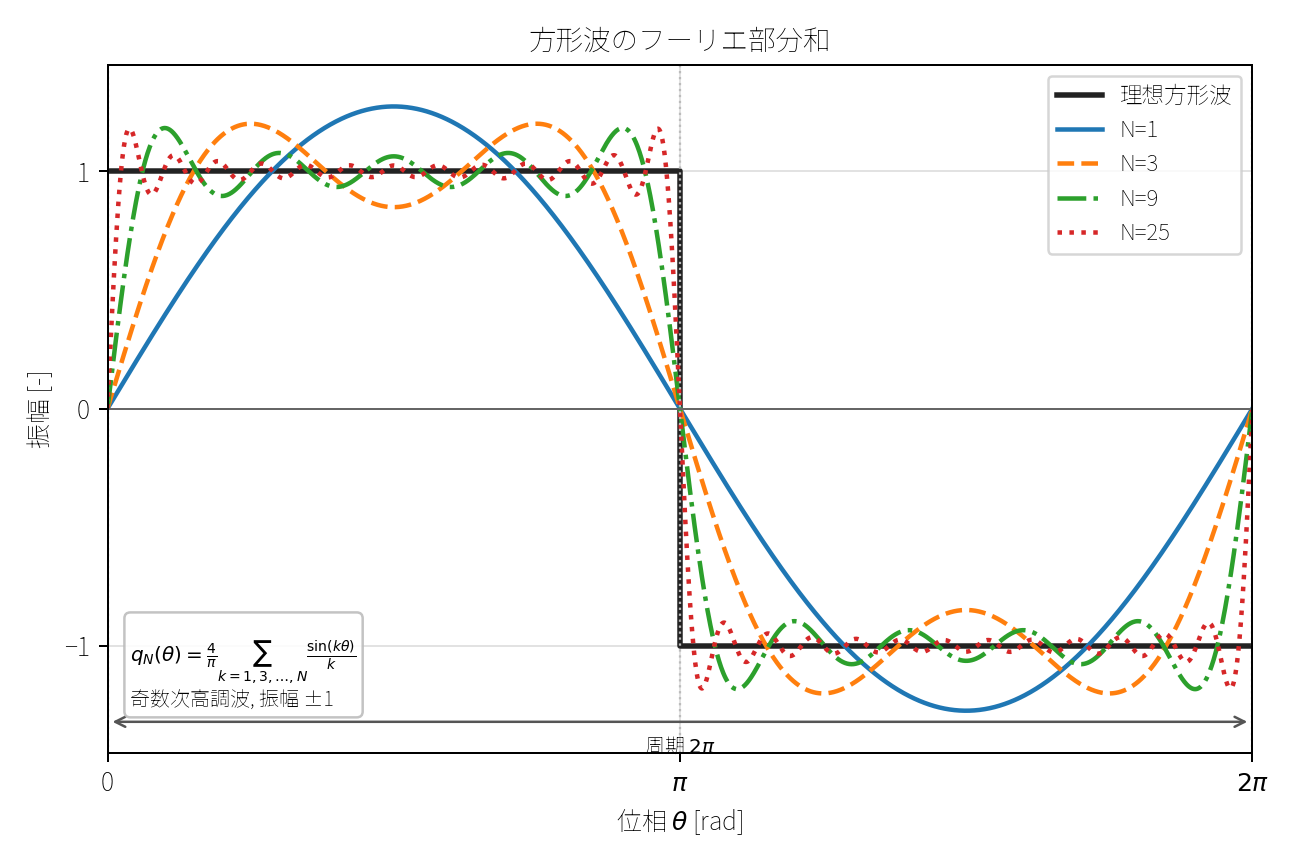
\includegraphics[width=0.88\linewidth,bb=0 0 1296 864]{figures/fourier_square_partial_sums.png}
\caption{周期 $2\pi$、振幅 $\pm1$ に正規化した方形波と、奇数次高調波 $k=1,3,\ldots,N$ だけを $N=1,3,9,25$ で打ち切ったフーリエ部分和。高い奇数次高調波ほど不連続点近傍の鋭い立上りを作るため、帯域制限をもつ制御対象や閉ループでは方形波指令や急な外乱が丸められ、帯域付近の位相遅れや共振が過渡応答として現れやすい。}
\label{fig:fourier-square-partial-sums}
\end{figure}

図\ref{fig:fourier-square-partial-sums} では、$N$ を増やすほど平坦部が $\pm1$ に近づき、不連続点の近くで急な変化が作られる。$N=1$ は基本波だけなので角は再現されず、波形全体が滑らかな正弦波として残る。$N=3$ や $N=9$ では低次の奇数次高調波が平坦部と立上りを作り始め、$N=25$ では高次成分によって立上りがさらに鋭くなる一方、不連続点近傍には部分和特有の振動が集中する。したがって理想的な方形波には、任意に高い奇数次高調波が必要である。制御対象や閉ループが $k=9$ 以上の成分をほとんど通過させないなら、出力は高次部分和ではなく低次部分和に近い形になり、方形波指令や急な外乱の角は有限の傾きをもつ丸い立上りへ変わる。帯域付近に大きな位相遅れや共振があれば、その丸められた立上りの後に遅れ、行き過ぎ、残留振動が時間波形として現れる。

\subsubsection{正弦波定常応答と伝達関数の虚軸評価}

線形時不変系では、各正弦波成分を個別に評価できる。安定な線形時不変系、または対象とする初期条件で過渡成分が減衰する線形時不変系に正弦波を入れると、過渡成分が消えた後の出力も同じ周波数の正弦波になる。入力を $u(t)=A\sin \omega t$ とする。ただし $A$ は振幅、$\omega\,[\mathrm{rad/s}]$ は角周波数である。このとき出力は
\begin{equation}
  y(t)=A\abs{G(j\omega)}\sin\{\omega t+\angle G(j\omega)\}
\end{equation}
で表せる。$G(j\omega)$ は伝達関数 $G(s)$ に $s=j\omega$ を代入したものである。安定で虚軸上の評価が収束する系では、$G(j\omega)$ が角周波数 $\omega$ の成分に対する複素倍率を与える。絶対値 $\abs{G(j\omega)}$ が入力振幅に対する出力振幅の比、偏角 $\angle G(j\omega)$ が入力正弦波に対する出力正弦波の位相差を表す。

一次遅れ $G(s)=K/(\tau s+1)$ について、ここでは $K>0$ とする。このとき
\begin{align}
  \abs{G(j\omega)}&=\frac{K}{\sqrt{1+(\tau\omega)^2}},\\
  \angle G(j\omega)&=-\tan^{-1}(\tau\omega).
\end{align}
低周波では入力がゆっくり変化するため出力はほぼ追従し、高周波では対象の応答遅れによりゲインが低下し位相が遅れる。時定数 $\tau$ が大きいほど、同じ $\omega$ でも $\tau\omega$ が大きくなるため、振幅低下と位相遅れが低い周波数から現れる。周波数応答は、目標値、ノイズ、振動成分が制御系を通過する際の振幅比と位相差を表す。

この情報は安定性、ロバスト性、ノイズ感度の評価に直結する。フィードバック系の閉ループ極は特性方程式で決まるが、開ループ $L(j\omega)$ のゲインと位相を周波数ごとに調べると、ゲイン増加、むだ時間、未モデル化共振、追加の位相遅れがゲイン余裕・位相余裕をどの帯域で減らすかを特定できる。一方、センサノイズは相補感度関数や制御入力の大きさを通じて出力変動、追従精度、アクチュエータ飽和余裕を制限する性能要因であり、飽和などの非線形実装効果を介する場合を除けば、線形解析上は閉ループ極を直接に不安定側へ動かさない。したがって、周波数応答は時間応答の代替ではなく、時間波形で観察した振動やオーバーシュートを、ゲイン余裕、位相余裕、帯域幅、感度関数、相補感度関数として定量化するための橋渡しである。

\subsection{ボード線図}

ボード線図は、横軸を対数目盛の角周波数 $\omega$ とし、上段にゲイン $20\log_{10}\abs{G(j\omega)}$、下段に位相 $\angle G(j\omega)$ を描く図である。ゲインを dB で表すと、伝達関数の積がゲイン線図では和になる。したがって
\begin{equation}
  G(s)=K\frac{(1+T_1s)(1+T_2s)}{s(1+\tau_1s)(1+\tau_2s)}
\end{equation}
のような形は、定数ゲイン、零点、積分器、一次遅れの寄与へ分解できる。

\subsubsection{因子分解によるボード線図の漸近作図}

漸近作図の目的は、厳密な数値計算を置き換えることではなく、どの周波数帯でどの因子が支配的かを図上で把握することである。ここでは各因子が無次元になるように正規化し、折点周波数を $\omega_b\,[\mathrm{rad/s}]$ と書く。1 decade は角周波数が 10 倍になる区間であり、ゲインの傾きは $\mathrm{dB/dec}$ で表す。

定数ゲイン $K$ は
\begin{equation}
  20\log_{10}\abs{K}
\end{equation}
だけゲイン線図を上下に移動させる。$K>0$ なら位相は $0^\circ$、$K<0$ なら全周波数で $180^\circ$ を加える。積分器と微分器は $s^q$ とまとめて書ける。係数側に必要な単位を含め、原点因子の周波数依存だけを評価するときは、基準角周波数 $\omega_0=1\,\mathrm{rad/s}$ で割って無次元化しておく。$q$ が正なら $q$ 個の微分器、負なら $-q$ 個の積分器であり、
\begin{align}
  20\log_{10}\abs{\left(\frac{j\omega}{\omega_0}\right)^q}
    &=20q\log_{10}\frac{\omega}{\omega_0},\\
  \angle (j\omega)^q
    &=90q^\circ
\end{align}
である。したがってゲイン傾きは $20q\,\mathrm{dB/dec}$ で、$1/s$ は $-20\,\mathrm{dB/dec}$ と $-90^\circ$、$s$ は $+20\,\mathrm{dB/dec}$ と $+90^\circ$ を与える。

左半平面にある実零点は
\begin{equation}
  F_z(s)=1+\frac{s}{\omega_z}
\end{equation}
と書ける。この因子の厳密なゲインと位相は
\begin{align}
  20\log_{10}\abs{F_z(j\omega)}
    &=10\log_{10}\left\{1+\left(\frac{\omega}{\omega_z}\right)^2\right\},\\
  \angle F_z(j\omega)
    &=\tan^{-1}\frac{\omega}{\omega_z}
\end{align}
である。$\omega\ll\omega_z$ では $F_z(j\omega)\simeq1$ なので $0\,\mathrm{dB}$、$\omega\gg\omega_z$ では $\abs{F_z(j\omega)}\simeq\omega/\omega_z$ なので $+20\,\mathrm{dB/dec}$ になる。よって $\omega_z$ を折点として、ゲイン傾きを $20\,\mathrm{dB/dec}$ 増やす。位相は $0^\circ$ から $+90^\circ$ へ移り、概略作図では $0.1\omega_z$ から $10\omega_z$ までを直線でつないで、$\omega_z$ で $+45^\circ$ と近似する。

左半平面の実極
\begin{equation}
  F_p(s)=\frac{1}{1+s/\omega_p}
\end{equation}
は実零点の逆数であるから、ゲインと位相の寄与は実零点の符号を反転したものになる。すなわち折点 $\omega_p$ を越えるとゲイン傾きは $20\,\mathrm{dB/dec}$ 減り、位相は $0^\circ$ から $-90^\circ$ へ移る。右半平面の実零点 $1-s/\omega_z$ や右半平面の実極 $1/(1-s/\omega_p)$ は、ゲイン線図の漸近線は左半平面因子と同じであるが、位相の符号が反対になる。したがって非最小位相零点や不安定極を含むときは、ゲインだけを見て位相余裕を推測してはならない。

二次因子は、減衰比 $\zeta>0$ と固有角周波数 $\omega_n$ を用いて
\begin{equation}
  F_2(s)=1+2\zeta\frac{s}{\omega_n}
    +\left(\frac{s}{\omega_n}\right)^2
\end{equation}
と書く。$0<\zeta<1$ なら共役複素極または零点に対応し、$\zeta\ge1$ なら二つの実一次因子へ分解してもよい。$r=\omega/\omega_n$ とおくと
\begin{align}
  F_2(j\omega)
    &=1-r^2+j2\zeta r,\\
  \abs{F_2(j\omega)}
    &=\sqrt{(1-r^2)^2+(2\zeta r)^2}.
\end{align}
二次零点 $F_2(s)$ は $\omega_n$ より十分低いところで $0\,\mathrm{dB}$、十分高いところで $+40\,\mathrm{dB/dec}$ となる。二次極 $1/F_2(s)$ は同じ折点で傾きが $40\,\mathrm{dB/dec}$ 減り、位相は $0^\circ$ から $-180^\circ$ へ移る。二次零点では位相の符号が逆になり、$0^\circ$ から $+180^\circ$ へ移る。$\omega=\omega_n$ では $F_2(j\omega_n)=j2\zeta$ なので、二次極の厳密なゲインは
\begin{equation}
  20\log_{10}\frac{1}{2\zeta}
  =-20\log_{10}(2\zeta)
\end{equation}
である。したがって小さい $\zeta$ では折点付近に山が現れ、二本の直線漸近線だけでは共振を評価できない。

一次因子の漸近線誤差は固定値として覚えられる。実零点で $x=\omega/\omega_z$ とおくと、ゲイン漸近線との差は
\begin{equation}
  e_z(x)=10\log_{10}(1+x^2)-\max\{0,20\log_{10}x\}
\end{equation}
である。折点 $x=1$ では $e_z(1)=10\log_{10}2\simeq3.01\,\mathrm{dB}$ であり、$x=0.1$ と $x=10$ では約 $0.043\,\mathrm{dB}$ まで小さくなる。実極の誤差は $-e_z(x)$ である。二次因子の折点誤差は $\zeta$ に依存し、二次極では $-20\log_{10}(2\zeta)$ が折点での厳密値になる。

以上を使うと、漸近作図の手順は明確になる。まず因子分解して折点周波数を小さい順に並べる。次に定数ゲインと原点因子から低周波側の高さと傾きを決める。折点を通過するたびに、実零点なら $+20$、実極なら $-20$、二次零点なら $+40$、二次極なら $-40$ を傾きに加える。位相線図は各因子の寄与を同じ周波数軸上で足し合わせる。最後に一次因子の折点で約 $3\,\mathrm{dB}$、二次因子では $\zeta$ に応じた誤差または共振ピークを補正して、漸近線と厳密線図のずれを評価する。

\begin{example}[積の形によるボード線図の漸近作図]
背景知識を必要としない例として、次の正規化された開ループを考える。$s$ と各折点周波数の単位は $\mathrm{rad/s}$ であり、原点因子も $\omega_0=1\,\mathrm{rad/s}$ で割って無次元化する。したがって定数 $5$ は無次元の倍率として扱える。
\begin{equation}
\begin{aligned}
  L(s)
  &=5\,\frac{1+s/\omega_z}{(s/\omega_0)(1+s/\omega_p)}\\
  &\quad{}\times
    \frac{1}{1+2\zeta s/\omega_n+(s/\omega_n)^2},\\
  \omega_0&=1\,\mathrm{rad/s},\quad
  \omega_p=0.2\,\mathrm{rad/s},\\
  \omega_z&=2\,\mathrm{rad/s},\quad
  \omega_n=20\,\mathrm{rad/s},\\
  \zeta&=0.5.
\end{aligned}
\end{equation}
因子は、定数ゲイン $5$、正規化積分器 $1/(s/\omega_0)$、実零点 $1+s/\omega_z$、実極 $1/(1+s/\omega_p)$、減衰比 $\zeta=0.5$ と固有角周波数 $20\,\mathrm{rad/s}$ の二次極である。折点は
\begin{equation}
  0.2,\qquad 2,\qquad 20
  \quad [\mathrm{rad/s}]
\end{equation}
の順に並ぶ。

低周波側の初期線分では定数ゲインが $20\log_{10}5\simeq14\,\mathrm{dB}$、正規化積分器が $-20\log_{10}(\omega/\omega_0)$、すなわち $-20\,\mathrm{dB/dec}$ の傾きを与える。この初期線分を $\omega=1\,\mathrm{rad/s}$ へ外挿した切片は約 $14\,\mathrm{dB}$ であるが、有効な区間は最初の折点 $0.2\,\mathrm{rad/s}$ より低い範囲である。たとえば $\omega=0.1\,\mathrm{rad/s}$ では積分器が $+20\,\mathrm{dB}$ を与え、初期漸近ゲインは約 $34\,\mathrm{dB}$ になる。その後、$\omega=0.2$ で実極により傾きは $-40\,\mathrm{dB/dec}$ へ変わるので、$\omega=1\,\mathrm{rad/s}$ の漸近値は実極の寄与 $-20\log_{10}(1/0.2)$ を含み約 $0\,\mathrm{dB}$ である。$\omega=2$ で実零点が加わり、傾きは $-20\,\mathrm{dB/dec}$ へ戻る。$\omega=20$ で二次極が加わり、傾きは $-60\,\mathrm{dB/dec}$ になる。

\begin{figure}[tb]
\centering
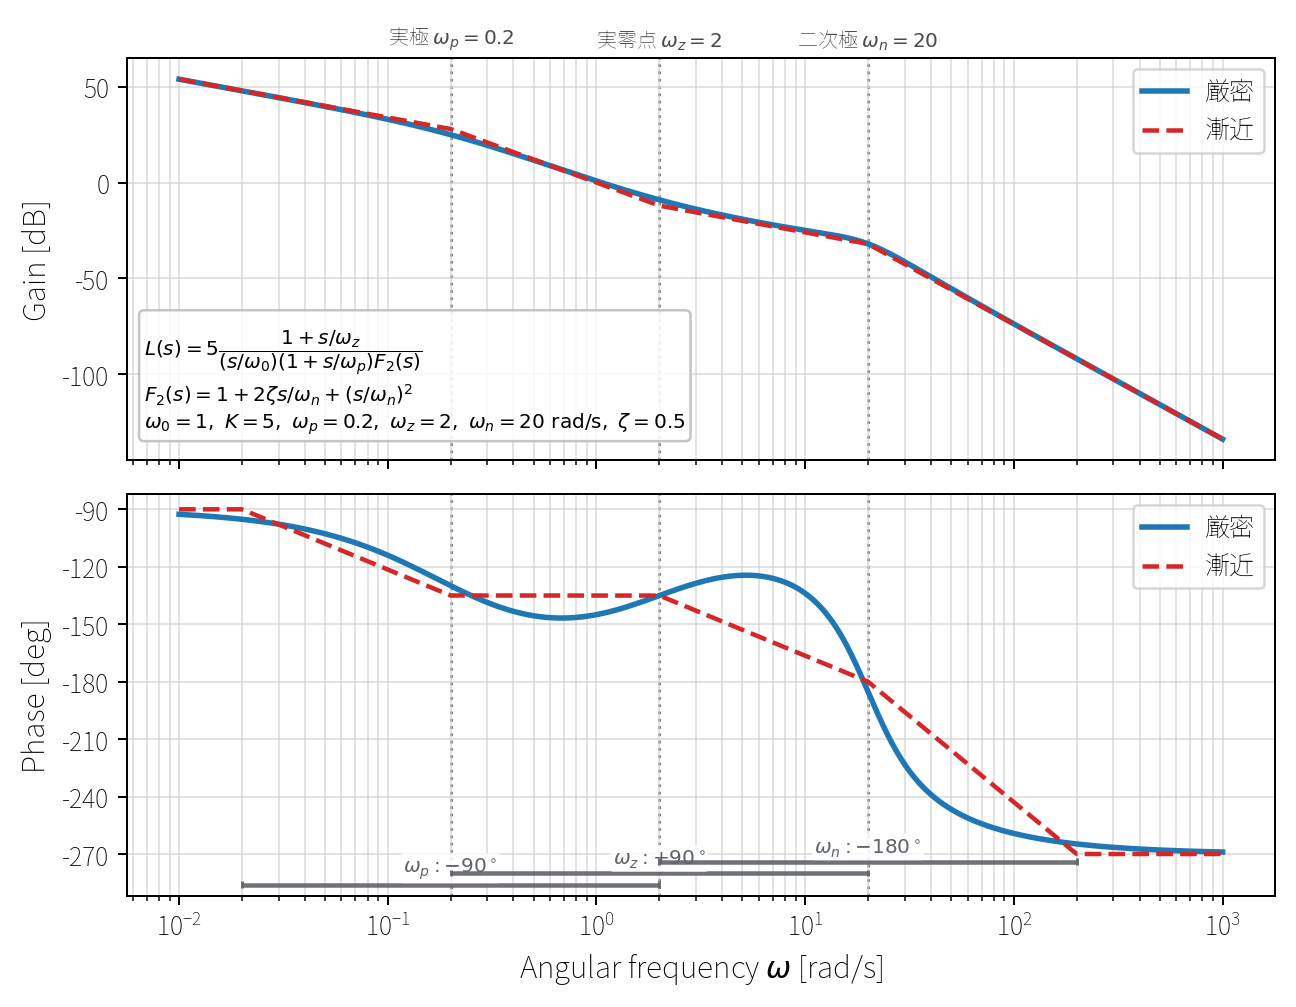
\includegraphics[width=0.88\linewidth,bb=0 0 1296 1007]{figures/bode_factor_example.png}
\caption{正規化された開ループ $L(s)$ のボード線図。$0.2\,\mathrm{rad/s}$ の実極でゲイン傾きが下がり、$2\,\mathrm{rad/s}$ の実零点で戻り、$20\,\mathrm{rad/s}$ の二次極でさらに低下する。破線の漸近線と実線の厳密線図を比べると、折点近傍の誤差と位相遷移を確認できる。}
\label{fig:bode-factor-example}
\end{figure}

位相は、正規化積分器の $-90^\circ$ から始める。実極 $1/(1+s/\omega_p)$ はおよそ $0.02$ から $2\,\mathrm{rad/s}$ の間でさらに $-90^\circ$ を加え、実零点 $1+s/\omega_z$ は $0.2$ から $20\,\mathrm{rad/s}$ の間で $+90^\circ$ を加える。二次極は $2$ から $200\,\mathrm{rad/s}$ 付近で $-180^\circ$ を加え、$\omega=20\,\mathrm{rad/s}$ では二次因子だけで $-90^\circ$ を与える。したがって高周波側の位相は、概略で
\begin{equation}
  -90^\circ-90^\circ+90^\circ-180^\circ=-270^\circ
\end{equation}
へ近づく。

折点近傍では直線だけを信用しすぎない。$\omega=0.2$ の実極は漸近線より約 $3\,\mathrm{dB}$ 低く、$\omega=2$ の実零点は約 $3\,\mathrm{dB}$ 高い。二次極は $\zeta=0.5$ なので $\omega=20$ での厳密な寄与が $20\log_{10}\{1/(2\zeta)\}=0\,\mathrm{dB}$ となり、折点そのものでは直線漸近線と一致する。しかし $\zeta$ がもっと小さければ、この周波数帯に共振の山が生じる。概略作図では、傾きの変化で全体の形を決め、折点誤差でゲイン値を補正する。
\end{example}

\subsubsection{余裕・交差周波数・帯域を仕様へ翻訳する}

本節では、設計仕様を開ループおよび閉ループの周波数応答指標として定義する。対象は単一入出力の単位負帰還系とし、開ループを
\begin{equation}
  L(s)=C(s)G(s)
\end{equation}
とおく。閉ループが安定で、評価する周波数で $L(j\omega)$ が定義できることを前提にする。開ループが右半平面極を持つ場合や交差周波数が複数ある場合には、余裕の値だけで安定性を断定せず、ナイキスト判別で閉ループ極の個数を確認する。

角周波数 $\omega$ の単位は $\mathrm{rad/s}$ である。周波数 $f\,[\mathrm{Hz}]$ で表すときは
\begin{equation}
  \omega=2\pi f
\end{equation}
を使う。ゲイン $\abs{L(j\omega)}$ は無次元の比であり、dB 表示では $20\log_{10}\abs{L(j\omega)}$ と書く。位相はラジアンまたは度で表す。むだ時間を含む式ではラジアンを用いる。

\begin{definition}[交差周波数と安定余裕]
ゲイン交差周波数 $\omega_{gc}$ は
\begin{equation}
  \abs{L(j\omega_{gc})}=1
\end{equation}
を満たす周波数である。これは dB 表示で $0\,\mathrm{dB}$ を横切る周波数である。位相交差周波数 $\omega_{pc}$ は、位相を連続につないで読んだとき
\begin{equation}
  \angle L(j\omega_{pc})=-\pi
  \qquad (-180^\circ)
\end{equation}
を満たす周波数である。ゲイン交差周波数での位相余裕を
\begin{equation}
  \phi_m=\pi+\angle L(j\omega_{gc})
\end{equation}
と定義する。度で表すなら $\phi_m=180^\circ+\angle L(j\omega_{gc})$ である。位相交差周波数でのゲイン余裕を
\begin{equation}
  g_m=\frac{1}{\abs{L(j\omega_{pc})}}
\end{equation}
と定義し、dB では
\begin{equation}
  G_{m,\mathrm{dB}}=20\log_{10}g_m
  =-20\log_{10}\abs{L(j\omega_{pc})}
\end{equation}
と表す。
\end{definition}

位相余裕の符号は、「あとどれだけ位相が遅れると $-180^\circ$ に達するか」を表すように取る。たとえば $\angle L(j\omega_{gc})=-135^\circ$ なら
\begin{equation}
  \phi_m=180^\circ-135^\circ=45^\circ
\end{equation}
である。正の位相余裕は、ゲイン交差周波数において位相が $-180^\circ$ に達していないことを示す。負の位相余裕は、同じ周波数で位相が $-180^\circ$ を越えていることを示す。ただし多重交差や不安定開ループ極がある場合には、この指標だけで閉ループ安定性を判定しない。

\begin{derivation}
ゲイン余裕が「何倍のゲイン増加に耐えるか」を表すことを式で見る。対象や制御器のゲインが見積もりより $k$ 倍になったとすると、開ループは $kL(s)$ になる。閉ループ特性方程式は
\begin{equation}
  1+kL(s)=0
\end{equation}
である。位相交差周波数では $L(j\omega_{pc})$ が負の実軸上にあり、
\begin{equation}
  L(j\omega_{pc})=-\abs{L(j\omega_{pc})}
\end{equation}
と書ける。境界的に $1+kL=0$ となる条件は
\begin{align}
  1-k\abs{L(j\omega_{pc})}&=0,\\
  k&=\frac{1}{\abs{L(j\omega_{pc})}}
\end{align}
である。したがって $g_m$ は、単純なゲイン増加に対する許容量を無次元倍率で表している。
\end{derivation}

位相余裕は、むだ時間の許容量の近似評価に用いられる。むだ時間 $\tau_d$ は開ループに $e^{-s\tau_d}$ を掛けるので、周波数 $\omega$ での追加位相遅れは
\begin{equation}
  \angle e^{-j\omega\tau_d}=-\omega\tau_d
\end{equation}
である。ゲイン交差周波数の近くで閉ループ安定性が決まると見なせるなら、許されるむだ時間の目安は
\begin{equation}
  \tau_{d,\max}\simeq\frac{\phi_m}{\omega_{gc}}
\end{equation}
となる。ただしこの式の $\phi_m$ はラジアンである。$\omega_{gc}$ が大きいほど、同一の位相余裕に対する許容むだ時間は短くなる。したがって、応答帯域を高く設定することと、むだ時間に対するロバスト性を増加させることは一般にトレードオフとなる。

閉ループの応答帯域は、相補感度
\begin{equation}
  T(s)=\frac{L(s)}{1+L(s)}
\end{equation}
の帯域幅により定義する。低周波で $T(0)\simeq 1$ なら、閉ループ帯域幅 $\omega_b$ は
\begin{equation}
  \abs{T(j\omega_b)}=\frac{1}{\sqrt{2}}\abs{T(0)}
\end{equation}
を初めて満たす周波数として定義する。これは低周波ゲインから
\begin{equation}
  20\log_{10}\frac{1}{\sqrt{2}}
  =-10\log_{10}2\simeq -3.01\,\mathrm{dB}
\end{equation}
下がる点である。$\omega_b$ より十分低い目標値成分はよく追従され、$\omega_b$ より高い成分は閉ループで減衰し始める。したがって、目標値や外乱の主成分を通したいなら $\omega_b$ をその周波数より上に置き、測定ノイズや未モデル化共振を入れたくないなら $\omega_b$ をそれらより十分低く置く。

一次閉ループ
\begin{equation}
  T_1(s)=\frac{1}{\tau_c s+1}
\end{equation}
では
\begin{equation}
  \abs{T_1(j\omega)}=\frac{1}{\sqrt{1+(\omega\tau_c)^2}}
\end{equation}
である。$\abs{T_1(j\omega_b)}=1/\sqrt{2}$ を代入すると
\begin{align}
  \frac{1}{\sqrt{1+(\omega_b\tau_c)^2}}&=\frac{1}{\sqrt{2}},\\
  1+(\omega_b\tau_c)^2&=2,\\
  \omega_b&=\frac{1}{\tau_c}
\end{align}
となる。一次応答の 10--90\% 立上り時間はおよそ $2.2\tau_c$、2\% 整定時間はおよそ $4\tau_c$ であるから、一次的に振る舞う閉ループでは
\begin{equation}
  t_r\simeq\frac{2.2}{\omega_b},
  \qquad
  T_s\simeq\frac{4}{\omega_b}
\end{equation}
という時間応答指標との近似対応が得られる。

閉ループゲインの最大値を共振ピークという。低周波ゲインが 1 に正規化された閉ループでは
\begin{equation}
  M_r=\max_{\omega\ge 0}\abs{T(j\omega)}
\end{equation}
で定義し、dB では $20\log_{10}M_r$ と表す。$M_r=1.3$ は約 $2.3\,\mathrm{dB}$ であり、対応する周波数成分の振幅比が 1.3 であることを表す。

二次標準閉ループ
\begin{equation}
  T_2(s)=\frac{\omega_n^2}{s^2+2\zeta\omega_n s+\omega_n^2}
\end{equation}
では、$r=\omega/\omega_n$ とおくと
\begin{align}
  \abs{T_2(j\omega)}^2
  &=\frac{\omega_n^4}{(\omega_n^2-\omega^2)^2+(2\zeta\omega_n\omega)^2}\\
  &=\frac{1}{(1-r^2)^2+(2\zeta r)^2}.
\end{align}
分母を
\begin{equation}
  D(r)=(1-r^2)^2+(2\zeta r)^2
  =1+(4\zeta^2-2)r^2+r^4
\end{equation}
とおく。共振ピークは $D(r)$ が最小になるところで生じるので、
\begin{align}
  \frac{\dd D}{\dd r}
  &=2(4\zeta^2-2)r+4r^3\\
  &=4r(r^2+2\zeta^2-1)
\end{align}
を 0 とおく。$r>0$ の解は
\begin{equation}
  r^2=1-2\zeta^2
\end{equation}
である。したがって $0<\zeta<1/\sqrt{2}$ のときだけ共振周波数
\begin{equation}
  \omega_r=\omega_n\sqrt{1-2\zeta^2}
\end{equation}
が存在し、そのピークは
\begin{equation}
  M_r=\frac{1}{2\zeta\sqrt{1-\zeta^2}}
\end{equation}
となる。$\zeta\ge 1/\sqrt{2}$ では山は低周波側の値を越えず、明確な共振ピークは現れない。

同じ二次支配の閉ループを開ループの位相余裕と結びつけるには、
\begin{equation}
  L(s)=\frac{T_2(s)}{1-T_2(s)}
  =\frac{\omega_n^2}{s(s+2\zeta\omega_n)}
\end{equation}
と見る。$x=\omega_{gc}/\omega_n$ とおくと、ゲイン交差条件は
\begin{align}
  1&=\abs{L(j\omega_{gc})}\\
  &=\frac{1}{x\sqrt{x^2+4\zeta^2}}
\end{align}
である。よって
\begin{equation}
  x^4+4\zeta^2x^2-1=0
\end{equation}
となり、正の解は
\begin{equation}
  x^2=-2\zeta^2+\sqrt{4\zeta^4+1}
\end{equation}
である。このとき開ループ位相は
\begin{equation}
  \angle L(j\omega_{gc})=-\frac{\pi}{2}-\tan^{-1}\frac{x}{2\zeta}
\end{equation}
だから、位相余裕は
\begin{equation}
  \phi_m=\tan^{-1}\frac{2\zeta}{x}
\end{equation}
となる。この関係は、支配極が二次標準形に近く、零点やむだ時間の影響が小さい場合に成立する近似である。一般の高次系では、位相余裕と共振ピークを閉ループ減衰性の評価指標として用いる。

\begin{example}[温度制御ループの周波数仕様]
熱容量を持つ加熱対象に積分動作を含む制御をかけ、対象の主時定数とセンサ遅れをまとめた候補開ループが
\begin{equation}
  L(s)=\frac{K}{s(1+s)(1+0.1s)}
\end{equation}
で近似できるとする。時間の単位は秒で、$K$ は開ループ全体が無次元になるように正規化されたゲインである。以下では、補償器の構成ではなく、候補開ループに対応する仕様値を計算する。

ゲイン交差周波数を $\omega_{gc}=0.7\,\mathrm{rad/s}$ 付近に置いた候補を考えると、
\begin{equation}
  K=0.7\sqrt{1+0.7^2}\sqrt{1+(0.1\cdot0.7)^2}
  \simeq 0.857
\end{equation}
で $\abs{L(j0.7)}=1$ となる。この周波数での位相は
\begin{align}
  \angle L(j0.7)
  &=-90^\circ-\tan^{-1}(0.7)-\tan^{-1}(0.07)\\
  &\simeq -90^\circ-35.0^\circ-4.0^\circ\\
  &\simeq -129^\circ
\end{align}
である。したがって位相余裕は
\begin{equation}
  \phi_m\simeq 180^\circ-129^\circ=51^\circ
\end{equation}
である。むだ時間余裕に換算すると
\begin{equation}
  \tau_{d,\max}\simeq
  \frac{51\pi/180}{0.7}
  \simeq 1.27\,\mathrm{s}
\end{equation}
である。

位相交差周波数は
\begin{equation}
  -90^\circ-\tan^{-1}\omega-\tan^{-1}(0.1\omega)=-180^\circ
\end{equation}
から求まる。すなわち
\begin{equation}
  \tan^{-1}\omega+\tan^{-1}(0.1\omega)=90^\circ
\end{equation}
である。二つの正の角の和が $90^\circ$ になる条件は、正接の加法公式の分母
\begin{equation}
  1-0.1\omega^2
\end{equation}
が 0 になることである。よって
\begin{equation}
  \omega_{pc}=\sqrt{10}\simeq 3.16\,\mathrm{rad/s}
\end{equation}
である。このとき
\begin{align}
  \abs{L(j\omega_{pc})}
  &=\frac{K}{\sqrt{10}\sqrt{1+10}\sqrt{1+0.1}}\\
  &=\frac{K}{11}\\
  &\simeq 0.0779
\end{align}
なので
\begin{align}
  g_m&\simeq 12.8,\\
  G_{m,\mathrm{dB}}&=20\log_{10}(12.8)\simeq 22.2\,\mathrm{dB}
\end{align}
である。この候補では、対象ゲインの変動よりも、位相遅れおよびむだ時間が安定余裕を制限する。

閉ループの相補感度は
\begin{equation}
  T(s)=\frac{K}{s(1+s)(1+0.1s)+K}
\end{equation}
である。直接代入して $\abs{T(j\omega)}=1/\sqrt{2}$ となる点を調べると、帯域幅はおよそ
\begin{equation}
  \omega_b\simeq 1.18\,\mathrm{rad/s}
\end{equation}
である。また $\abs{T(j\omega)}$ の山はおよそ
\begin{equation}
  M_r\simeq 1.16
  \qquad (20\log_{10}M_r\simeq 1.3\,\mathrm{dB})
\end{equation}
である。この候補に対する仕様値は、帯域幅 $\omega_b\simeq1.18\,\mathrm{rad/s}$、位相余裕 $\phi_m\simeq51^\circ$、むだ時間余裕 $\tau_{d,\max}\simeq1.27\,\mathrm{s}$、共振ピーク約 $1.3\,\mathrm{dB}$ である。
\end{example}

仕様値は対象、センサノイズ、モデル誤差、むだ時間、許容振動に依存する。位相余裕、ゲイン余裕、帯域幅、共振ピークは、同一の閉ループ伝達特性から定義される指標であり、独立に指定できる量ではない。

\subsection{位相補償器の仕様設計}

ボード線図による古典設計では、制御器 $C(s)$ を選んで開ループ
\begin{equation}
  L(s)=C(s)G(s)
\end{equation}
のゲイン交差周波数、位相余裕、低周波ゲインを同時に調整する。ここでは単一入出力の単位負帰還系を対象とし、閉ループ安定性は最終的にナイキスト判別または閉ループ極で確認するものとする。開ループが不安定極や非最小位相零点を持つ場合、以下の設計式は候補を作るための近似であり、余裕の値だけで安定性を保証しない。

ここで調整する量は、時間応答の観察量と対応している。低周波ゲインは一定外乱やゆっくり変化する目標に対する残留誤差を支配し、ゲイン交差周波数は立上り時間や外乱抑制の速さのおおよその尺度になる。位相余裕は同じ交差周波数でどれだけ振動的な応答になるかを示し、余裕が小さいとオーバーシュート、整定時間の増大、アクチュエータ入力の振動として現れる。一方、交差周波数より十分高い周波数では、センサノイズや未モデル化の弾性モード、むだ時間、サンプリング遅れを増幅しないことが重要である。したがって、補償器の零点と極は、単に式を満たす位置ではなく、低周波の誤差、交差周波数の余裕、高周波のロバスト性がボード線図上で同時に確認できる位置に置く。

定常偏差仕様は、低周波における開ループの大きさを指定する。開ループが原点極を $q$ 個持つ型 $q$ の系で、目標入力が $q$ 次までの多項式信号であるとき、対応する誤差定数は
\begin{equation}
  K_e=\lim_{s\to0}s^q L(s)
\end{equation}
で表せる。$q=0$ では位置誤差定数 $K_p$、$q=1$ では速度誤差定数 $K_v$、$q=2$ では加速度誤差定数 $K_a$ である。たとえば型 1 の系に単位傾斜入力を加えると、定常偏差は
\begin{equation}
  e_{ss}=\frac{1}{K_v}
\end{equation}
である。したがって、低周波ゲインを大きくすると定常偏差は小さくなる。一方、交差周波数付近のゲインを不用意に上げると帯域幅が増え、位相余裕が減り、高周波ノイズや未モデル化ダイナミクスの影響を受けやすくなる。位相進み補償、位相遅れ補償、遅れ進み補償は、この低周波と交差周波数の要求を分けて調整するために用いられる。

\subsubsection{位相進み補償器}

位相進み補償器を
\begin{equation}
  C_{\mathrm{lead}}(s)
  =K_c\frac{1+Ts}{1+\alpha Ts},
  \qquad 0<\alpha<1,\quad T>0
\end{equation}
とおく。零点は $\omega_z=1/T$、極は $\omega_p=1/(\alpha T)$ にあり、$\omega_z<\omega_p$ である。周波数応答の位相寄与は
\begin{equation}
  \phi_{\mathrm{lead}}(\omega)
  =\tan^{-1}(\omega T)-\tan^{-1}(\alpha\omega T)
\end{equation}
であり、零点と極の間で正になる。$x=\omega T$ とおいて $\phi_{\mathrm{lead}}$ を $\log \omega$ で微分すると、最大位相進みは
\begin{equation}
  \omega_m=\frac{1}{T\sqrt{\alpha}}
\end{equation}
で生じる。この周波数は零点と極の幾何平均である。最大位相進みを $\phi_{\max}$ と書くと
\begin{align}
  \sin\phi_{\max}
  &=\frac{1-\alpha}{1+\alpha},\\
  \alpha
  &=\frac{1-\sin\phi_{\max}}{1+\sin\phi_{\max}}
\end{align}
である。また $\omega_m$ における大きさは
\begin{equation}
  \abs{\frac{1+j\omega_m T}{1+j\alpha\omega_m T}}
  =\frac{1}{\sqrt{\alpha}}
\end{equation}
である。したがって位相進み補償器は、交差周波数付近で正の位相を与えると同時に、同じ周波数帯のゲインも上げる。ボード線図では、零点の後で大きさの傾きが上向き、極の後で元の傾きに戻り、その間で位相が持ち上がる。この持ち上がりを交差周波数に合わせると、時間応答では立上りを速くしながら、位相余裕の不足による振動やオーバーシュートを抑える方向に働く。ただし高周波側では
\begin{equation}
  \lim_{\omega\to\infty}
  \abs{\frac{1+j\omega T}{1+j\alpha\omega T}}
  =\frac{1}{\alpha}
\end{equation}
となるため、測定ノイズが制御入力へ伝わりやすくなる。さらに、対象モデルに含めていない高周波の機械共振、電流制御の遅れ、サンプリングに起因する位相遅れがあると、交差周波数を上げた設計ほどそれらの影響を受けやすい。位相進みを入れた後のボード線図では、目標交差周波数で位相余裕が増えていることだけでなく、高周波側のゲイン上昇がセンサノイズ帯域や未モデル化モードの近くまで及んでいないことを同時に読む。必要な位相進みが大きすぎる場合には、交差周波数を下げる、複数段の位相進みへ分ける、または仕様そのものを見直す。

目標ゲイン交差周波数を $\omega_c^\star$、目標位相余裕を $\phi_m^\star$ とする。まず対象だけの位相
\begin{equation}
  \phi_G=\angle G(j\omega_c^\star)
\end{equation}
を計算し、補償前にその周波数で得られる位相余裕を $\pi+\phi_G$ と読む。この値は、目標帯域で閉ループがどれだけ振動しやすいかを示す未補償の証拠である。位相遅れ補償や未モデル化遅れに対する余裕を $\delta_\phi\ge0$ と見込むと、必要な位相進みは
\begin{equation}
  \phi_d
  =\phi_m^\star-\{\pi+\phi_G\}+\delta_\phi
\end{equation}
である。角度を度で扱う場合は、同じ式の $\pi$ を $180^\circ$ に置き換える。$0<\phi_d<\pi/2$ の範囲で $\alpha$ を
\begin{equation}
  \alpha=\frac{1-\sin\phi_d}{1+\sin\phi_d}
\end{equation}
から決め、最大位相進みが目標交差周波数に来るように
\begin{equation}
  T=\frac{1}{\omega_c^\star\sqrt{\alpha}}
\end{equation}
を選ぶ。最後にゲイン条件
\begin{equation}
  \abs{K_c C_{\mathrm{lead},0}(j\omega_c^\star)G(j\omega_c^\star)}=1
\end{equation}
から $K_c$ を定める。ここで $C_{\mathrm{lead},0}$ は $K_c$ を除いた位相進み因子である。このゲイン調整は、位相進みによる大きさの山を含めた後でも、開ループの $0\,\mathrm{dB}$ 交差を狙った帯域に戻す操作である。最大位相点を交差周波数に合わせた場合、
\begin{equation}
  K_c
  =\frac{\sqrt{\alpha}}{\abs{G(j\omega_c^\star)}}
\end{equation}
である。

\subsubsection{位相遅れ補償器}

位相遅れ補償器は、交差周波数を大きく動かさずに低周波ゲインを増やすために用いる。交差周波数近傍の大きさがほぼ $K_c$ になるように正規化して
\begin{equation}
  C_{\mathrm{lag}}(s)
  =K_c\beta\frac{1+T_\ell s}{1+\beta T_\ell s},
  \qquad \beta>1,\quad T_\ell>0
\end{equation}
と書く。極は $\omega_p=1/(\beta T_\ell)$、零点は $\omega_z=1/T_\ell$ にあり、$\omega_p<\omega_z$ である。位相寄与は
\begin{equation}
  \phi_{\mathrm{lag}}(\omega)
  =\tan^{-1}(\omega T_\ell)
  -\tan^{-1}(\beta\omega T_\ell)
\end{equation}
であり、極と零点の間で負になる。一方、低周波と高周波の大きさは
\begin{align}
  \lim_{\omega\to0}\abs{C_{\mathrm{lag}}(j\omega)}
    &=K_c\beta,\\
  \lim_{\omega\to\infty}\abs{C_{\mathrm{lag}}(j\omega)}
    &=K_c
\end{align}
である。したがって、低周波の誤差定数を $\beta$ 倍しながら、交差周波数が零点より十分高ければ交差周波数近傍のゲインをほぼ保てる。これは、整定後に残る傾斜入力誤差や一定外乱の偏差を小さくする一方で、閉ループ帯域幅を大きく変えない設計である。時間応答では、位相遅れ補償だけで立上りを速くするのではなく、低周波の追従誤差をゆっくり押し下げる効果として現れる。

位相遅れ補償の設計では、まず位相余裕と交差周波数の仕様を満たす候補 $L_0(s)$ を作る。そこで得られる誤差定数を
\begin{equation}
  K_{e0}=\lim_{s\to0}s^q L_0(s)
\end{equation}
とし、要求値を $K_e^\star$ とすれば、低周波ゲイン倍率は
\begin{equation}
  \beta\ge\frac{K_e^\star}{K_{e0}}
\end{equation}
から決める。位相遅れを小さくするため、零点を目標交差周波数より十分低く置く。ボード線図では、低周波側で大きさが $\beta$ 倍だけ持ち上がり、零点より十分高い交差周波数では大きさがほぼ元に戻り、負の位相の谷が交差周波数から離れていることを確認する。たとえば $n=5$ から $10$ 程度を選び、
\begin{equation}
  \omega_z=\frac{\omega_c^\star}{n},
  \qquad
  \omega_p=\frac{\omega_z}{\beta}
\end{equation}
とすると
\begin{equation}
  T_\ell=\frac{1}{\omega_z}
  =\frac{n}{\omega_c^\star}
\end{equation}
である。$\omega_c^\star$ における位相遅れ
\begin{equation}
  \tan^{-1}n-\tan^{-1}(\beta n)
\end{equation}
が許容できるかを確認し、必要なら $n$ を大きくする。ただし $n$ を大きくしすぎると補償の折点が非常に低くなり、定常偏差の改善が現れるまでの時間が長くなる。すなわち、ボード線図上では交差周波数を保てていても、時間波形では低周波誤差がゆっくり残る長い尾として観測される。

\subsubsection{遅れ進み補償器の設計手順}

遅れ進み補償器は
\begin{equation}
  C_{\mathrm{leadlag}}(s)
  =K_c
  \frac{1+T_ds}{1+\alpha T_ds}
  \beta\frac{1+T_\ell s}{1+\beta T_\ell s},
  \qquad 0<\alpha<1,\quad \beta>1
\end{equation}
のように、位相進み因子と位相遅れ因子を直列に置いたものである。位相進み因子は主に位相余裕と交差周波数を調整し、位相遅れ因子は主に低周波誤差定数を調整する。

仕様から設計する基本手順は次の通りである。第一に、時間応答とロバスト性の要求から目標交差周波数 $\omega_c^\star$ と目標位相余裕 $\phi_m^\star$ を決める。$\omega_c^\star$ は閉ループ帯域幅と同じ程度の量であり、速い応答を求めるほど大きくなるが、むだ時間余裕、ノイズ、未モデル化高周波モードに対する余裕は小さくなる。このため、立上り時間だけから $\omega_c^\star$ を決めるのではなく、観測されたセンサノイズの帯域、アクチュエータが追従できる周波数、モデル同定で信頼できる周波数範囲を合わせて上限を置く。第二に、$G(j\omega_c^\star)$ の位相から必要な位相進み $\phi_d$ を求め、$\alpha$ と $T_d$ を決める。第三に、$\omega_c^\star$ で
\begin{equation}
  \abs{L(j\omega_c^\star)}=1
\end{equation}
となるように $K_c$ を定める。第四に、得られた低周波誤差定数が不足するなら $\beta$ を選び、位相遅れ因子の零点と極を $\omega_c^\star$ より十分低い周波数に置く。最後に、位相遅れ因子の実際の大きさと位相を含めて $K_c$、$\omega_{gc}$、$\phi_m$、誤差定数を再計算する。この再計算は、数値の帳尻合わせではなく、低周波の誤差改善、交差周波数での余裕、高周波のノイズ抑制が同じ開ループ線図で両立しているかを確認する工程である。

この手順は一回の計算で終わるとは限らない。位相進みを強くすると交差周波数が高くなり、閉ループ帯域幅も増える。帯域幅の増加は目標値追従と外乱抑制を速くする一方で、測定ノイズを相補感度 $T(s)$ から出力や入力へ通しやすくする。位相遅れは低周波ゲインを増やして定常偏差を減らすが、折点を交差周波数に近づけると位相余裕を削る。したがって、ボード線図上では「低周波で大きいループゲイン、交差周波数で十分な位相余裕、高周波で小さい相補感度」という三つの要求を同時に満たすように折点を配置する。

\begin{example}[遅れ進み補償器による周波数仕様設計]
正規化された位置制御対象
\begin{equation}
  G(s)=\frac{1}{s(s+1)}
\end{equation}
を単位負帰還で制御する。仕様を、速度誤差定数
\begin{equation}
  K_v\ge 50\,\mathrm{s^{-1}},
\end{equation}
目標ゲイン交差周波数
\begin{equation}
  \omega_c^\star=5\,\mathrm{rad/s},
\end{equation}
位相余裕
\begin{equation}
  \phi_m\ge50^\circ
\end{equation}
とする。この対象は型 1 なので、単位傾斜入力に対する定常偏差は $e_{ss}=1/K_v$ で評価できる。したがって、ここでの設計は、ランプ状に変化する位置指令へ残る低周波誤差を小さくしつつ、$5\,\mathrm{rad/s}$ 付近の位相余裕で振動的な応答を抑えることを同時に検証する例である。

まず $\omega=5$ における対象の周波数応答を求める。
\begin{align}
  \abs{G(j5)}
  &=\frac{1}{5\sqrt{1+5^2}}
    \simeq 0.0392,\\
  \angle G(j5)
  &=-90^\circ-\tan^{-1}5
    \simeq -168.7^\circ
\end{align}
である。交差周波数を $5\,\mathrm{rad/s}$ に置いたとき、対象だけでは位相余裕が約 $11.3^\circ$ しかない。これは、同じ帯域までゲインを上げるだけでは閉ループが振動的になり、目標追従の速さを得ても整定が悪化することを示すボード線図上の証拠である。位相遅れ補償で数度の位相損失が生じることを見込み、位相進み補償器に
\begin{equation}
  \phi_d=45^\circ
\end{equation}
を割り当てる。すると
\begin{align}
  \alpha
  &=\frac{1-\sin45^\circ}{1+\sin45^\circ}
    \simeq 0.172,\\
  T_d
  &=\frac{1}{5\sqrt{0.172}}
    \simeq 0.483\,\mathrm{s}
\end{align}
である。位相進み因子は
\begin{equation}
  C_{\mathrm{lead},0}(s)
  =\frac{1+0.483s}{1+0.0828s}
\end{equation}
となり、$5\,\mathrm{rad/s}$ での大きさは $1/\sqrt{\alpha}\simeq2.41$、位相は $45^\circ$ である。この数値は、位相余裕を増やす効果と同時に、交差周波数付近の大きさを約 $7.6\,\mathrm{dB}$ 持ち上げる効果を持つことを意味する。したがって、後で $K_c$ を調整して $0\,\mathrm{dB}$ 交差を保ち、帯域幅を意図した位置に戻す必要がある。

次に定常偏差仕様を満たす。位相進み因子だけで交差周波数を合わせると、必要ゲインはおよそ
\begin{equation}
  K_c\simeq
  \frac{1}{0.0392\cdot2.41}
  \simeq 10.6
\end{equation}
である。この段階の速度誤差定数は、$\lim_{s\to0}sK_cC_{\mathrm{lead},0}(s)G(s)=K_c$ より約 $10.6\,\mathrm{s^{-1}}$ であり、要求値 $50\,\mathrm{s^{-1}}$ に届かない。位相進みだけでは、振動性と帯域幅の条件は改善できても、ランプ追従に残る低周波誤差は十分に下がらない。したがって位相遅れ補償で低周波ゲインを約 5 倍にする。$\beta=5$ とし、零点を交差周波数の 1 decade 下に置いて
\begin{equation}
  \omega_z=0.5\,\mathrm{rad/s},
  \qquad
  \omega_p=0.1\,\mathrm{rad/s}
\end{equation}
とする。これは $T_\ell=2\,\mathrm{s}$ に対応し、
\begin{equation}
  C_{\mathrm{lag},0}(s)
  =5\frac{1+2s}{1+10s}
\end{equation}
である。

$5\,\mathrm{rad/s}$ における位相遅れ因子の大きさと位相は
\begin{align}
  \abs{C_{\mathrm{lag},0}(j5)}
  &=5\frac{\sqrt{1+10^2}}{\sqrt{1+50^2}}
    \simeq 1.005,\\
  \angle C_{\mathrm{lag},0}(j5)
  &=\tan^{-1}10-\tan^{-1}50
    \simeq -4.6^\circ
\end{align}
である。この値から、位相遅れ因子は低周波ゲインを増やしながら、目標交差周波数では大きさをほぼ変えず、位相余裕を約 $4.6^\circ$ だけ消費することが分かる。したがって、両方の補償因子を含めたゲイン条件から
\begin{equation}
  K_c=
  \frac{1}
  {0.0392\cdot2.41\cdot1.005}
  \simeq 10.5
\end{equation}
を得る。設計された制御器は
\begin{equation}
  C(s)=10.5
  \frac{1+0.483s}{1+0.0828s}
  \;5\frac{1+2s}{1+10s}
\end{equation}
である。

この制御器に対して、$5\,\mathrm{rad/s}$ での開ループ位相は
\begin{align}
  \angle L(j5)
  &\simeq -168.7^\circ+45.0^\circ-4.6^\circ\\
  &\simeq -128.3^\circ
\end{align}
である。したがって位相余裕は
\begin{equation}
  \phi_m\simeq 180^\circ-128.3^\circ=51.7^\circ
\end{equation}
となり、仕様を満たす。対象だけの $11.3^\circ$ から $51.7^\circ$ へ余裕が増えたので、同じ $5\,\mathrm{rad/s}$ の帯域を保ったまま、時間応答の振動性を小さくする方向に補償できている。速度誤差定数は
\begin{align}
  K_v
  &=\lim_{s\to0}sC(s)G(s)\\
  &=10.5\cdot5\\
  &\simeq52.6\,\mathrm{s^{-1}}
\end{align}
であり、単位傾斜入力に対する定常偏差は $e_{ss}\simeq0.019$ である。

ボード線図上では、位相進み因子が $5\,\mathrm{rad/s}$ 付近で位相余裕を増やし、位相遅れ因子が $0.1$ から $0.5\,\mathrm{rad/s}$ の低周波側でループゲインを持ち上げている。位相遅れ因子は交差周波数でほぼ $0\,\mathrm{dB}$ なので帯域幅を大きく変えない。このため、時間応答では低周波のランプ追従誤差が $e_{ss}\simeq0.019$ まで小さくなり、交差周波数に対応する速さはおおむね維持される。一方、位相進み因子の高周波ゲインは $1/\alpha\simeq5.8$ 倍であるため、センサノイズが大きい系では入力の高周波成分を別途確認する必要がある。さらに、$5\,\mathrm{rad/s}$ より上の周波数に未モデル化の共振や遅れがある場合、相補感度の山がその帯域に重ならないことを確認しなければならない。この例の設計値は、位相余裕、交差周波数、定常偏差を同時に満たす候補であり、最終的には閉ループ極、相補感度、入力振幅制限を合わせて評価する。
\end{example}

\subsection{ナイキスト線図}

単位負帰還系の閉ループ伝達関数は
\begin{equation}
  T(s)=\frac{L(s)}{1+L(s)}
\end{equation}
である。したがって閉ループの安定性は、特性方程式
\begin{equation}
  1+L(s)=0
\end{equation}
の根が右半平面に存在するかどうかで決まる。ボード線図の安定余裕は、点 $-1$ への近さを周波数ごとに評価する指標であった。ナイキスト線図はさらに一歩進めて、複素平面上の曲線が点 $-1$ を何回囲むかから、閉ループ右半平面極の個数そのものを数える。

以下では $L(s)$ を実係数の有理関数とし、虚軸上に開ループ極を持たず、調べる閉ループがちょうど安定限界にない、すなわち $1+L(j\omega)\ne0$ であると仮定する。虚軸上に積分器や共振極がある場合には、虚軸を小半円で避ける修正版のナイキスト経路を使う。本書では、右半平面を囲むナイキスト経路を、虚軸上で $-jR$ から $jR$ へ進み、右半平面の大半円で $jR$ から $-jR$ へ戻る向きに取る。この向きは右半平面を時計回りに囲む向きである。

\begin{definition}[囲み数の符号規約]
開ループ $L(s)$ の右半平面極の個数を $P$、閉ループ特性方程式 $1+L(s)=0$ の右半平面根の個数を $Z$ とする。ナイキスト線図が点 $-1$ を時計回りに囲む回数を $N$ と数える。反時計回りの囲みは負として数える。したがって、点 $-1$ を反時計回りに 1 回囲む場合は $N=-1$ である。
\end{definition}

この符号規約の下で、ナイキスト安定判別は
\begin{equation}
  Z=N+P
\end{equation}
と書ける。閉ループ安定性には $Z=0$ が必要十分であるから、開ループが安定で $P=0$ なら $N=0$、すなわち点 $-1$ を囲まないことが必要である。一方、開ループに右半平面極があるときは違う。たとえば $P=1$ なら、閉ループを安定にするには $N=-1$、すなわち点 $-1$ を反時計回りに 1 回囲む必要がある。

ここで数えている $Z$ は抽象的な複素解析上の個数ではなく、時間応答に現れる発散モードの個数である。閉ループ極 $s=\sigma+j\omega$ は過渡応答に $e^{\sigma t}$ と角周波数 $\omega$ の振動成分を与えるため、$Z>0$ ならどこかの初期誤差や外乱成分が時間とともに増幅される。したがってナイキスト線図の囲みは、周波数平面の作図を、時系列での減衰・持続振動・発散へ結び付ける安定性の証拠になる。

\begin{derivation}
偏角原理の考え方を、閉ループ特性関数
\begin{equation}
  F(s)=1+L(s)
\end{equation}
へ適用する。$F(s)$ の零点は閉ループ特性方程式の根であり、$F(s)$ の極は、約分で隠れていない開ループ $L(s)$ の極である。右半平面を時計回りに囲むナイキスト経路を $\Gamma$ とすると、$s$ が $\Gamma$ を一周するときの $F(s)$ の偏角変化は
\begin{equation}
  \Delta_\Gamma \arg F(s)=-2\pi(Z-P)
\end{equation}
である。右半平面内の零点は時計回り経路に対して $-2\pi$ の寄与を持ち、極は符号が反対になるためである。

ここで $F(s)=1+L(s)$ は、$L(s)$ のナイキスト線図を複素平面で右へ 1 だけ平行移動したものである。したがって、$F(s)$ が原点を囲む回数は、$L(s)$ が点 $-1$ を囲む回数と等しい。時計回りの囲み数を
\begin{equation}
  N=-\frac{1}{2\pi}\Delta_\Gamma \arg F(s)
\end{equation}
と定義したので
\begin{equation}
  N=Z-P
\end{equation}
であり、整理すると $Z=N+P$ を得る。
\end{derivation}

実係数の伝達関数では $L(-j\omega)=\overline{L(j\omega)}$ であるため、負の周波数側のナイキスト線図は正の周波数側の鏡映になる。ただし安定判別で数えるのは、正の周波数だけの曲線ではなく、負の周波数、正の周波数、大半円の像を合わせた閉じた曲線である。

\begin{example}[不安定開ループ極を持つナイキスト判別]
開ループを
\begin{equation}
  L(s)=\frac{2}{s-1}
\end{equation}
とする。これは $s=1$ に右半平面極を 1 個持つので
\begin{equation}
  P=1
\end{equation}
である。虚軸上では
\begin{align}
  L(j\omega)
  &=\frac{2}{-1+j\omega}\\
  &=\frac{2(-1-j\omega)}{1+\omega^2}\\
  &=-\frac{2}{1+\omega^2}
    -j\frac{2\omega}{1+\omega^2}
\end{align}
である。$L(j\omega)=x(\omega)+jy(\omega)$ とおくと
\begin{equation}
  x(\omega)=-\frac{2}{1+\omega^2},
  \qquad
  y(\omega)=-\frac{2\omega}{1+\omega^2}
\end{equation}
であり、
\begin{align}
  \{x(\omega)+1\}^2+y(\omega)^2
  &=
  \left(\frac{\omega^2-1}{1+\omega^2}\right)^2
  +
  \left(\frac{2\omega}{1+\omega^2}\right)^2\\
  &=1
\end{align}
を満たす。したがって虚軸部分の像は、中心 $-1$、半径 1 の円である。

$\omega$ を $-\infty$ から $+\infty$ へ増やすと、$L(j\omega)$ は原点近くの上側から出発し、$\omega=0$ で $-2$ を通り、原点近くの下側へ戻る。中心 $-1$ から見た偏角は $0$ から $\pi$ を通って $2\pi$ へ増えるので、点 $-1$ を反時計回りに 1 回囲む。大半円上では $L(s)\to0$ であり、その像は原点近くに縮むため、点 $-1$ の囲み数を変えない。よって本書の符号規約では
\begin{equation}
  N=-1
\end{equation}
である。

ナイキスト判別から
\begin{equation}
  Z=N+P=-1+1=0
\end{equation}
となる。閉ループ右半平面極は存在せず、閉ループは安定である。実際に直接計算しても
\begin{align}
  1+\frac{2}{s-1}&=0,\\
  \frac{s+1}{s-1}&=0
\end{align}
より閉ループ極は $s=-1$ であり、右半平面にはない。

この直接計算は、囲み数の結果を時間応答で読み替えている。閉ループ極が $-1$ にあるため、初期値や外乱で生じた過渡成分は $e^{-t}$ に比例して減衰する。ナイキスト線図が安定と判定したことは、単に曲線が条件を満たすという意味ではなく、この一次モードが右半平面から左半平面へ移り、発散しない応答になったことを表している。

同じ形を
\begin{equation}
  L_K(s)=\frac{K}{s-1}
\end{equation}
として見ると、閉ループ極は $s=1-K$ である。$K=1$ では $s=0$ となり、ナイキスト線図は $\omega=0$ でちょうど点 $-1$ を通る。$K>1$ では点 $-1$ を反時計回りに 1 回囲み、$Z=0$ で安定である。$0<K<1$ では点 $-1$ を囲まず、$N=0$、$Z=1$ となって不安定である。不安定な開ループ極がある場合、「点 $-1$ を囲まない」ことは安定条件ではなく、必要な反時計回りの囲みを失っていることを意味する。
\end{example}

\wfig{frequency-design-examples} 上左は、この不安定開ループ極を持つ一次例でゲインだけを変えたナイキスト線図である。$K=0.6$ の曲線は点 $-1$ を囲まず、$K=1$ では曲線が点 $-1$ を通って安定限界に乗る。$K=2$ では負の周波数から正の周波数へ進む向きで点 $-1$ を反時計回りに 1 回囲むので、本書の符号規約では $N=-1$ となり、$P=1$ と合わせて $Z=0$ が得られる。囲み数は曲線の形だけでなく、開ループ不安定極の個数と向きの規約を同時に読んで決まる。この図の三つの曲線は、同じ数式の時間応答が $K=0.6$ で $e^{0.4t}$ に比例して発散し、$K=1$ で減衰しない境界に乗り、$K=2$ で $e^{-t}$ に比例して減衰することを、周波数応答だけから分けている。

この例は、ゲイン余裕と位相余裕の解釈にも注意を与える。$L(s)=2/(s-1)$ では
\begin{equation}
  \abs{L(j\omega)}=\frac{2}{\sqrt{1+\omega^2}}
\end{equation}
なので、ゲイン交差周波数は
\begin{equation}
  \omega_{gc}=\sqrt{3}
\end{equation}
である。このとき位相は $-120^\circ$ であり、形式的な位相余裕は $60^\circ$ である。一方、位相が $-180^\circ$ となるのは $\omega=0$ で、そのとき $\abs{L(j0)}=2$ である。境界に達するゲイン倍率は $1/2$ であり、この系ではゲインを 2 倍まで増やせるという意味ではなく、ゲインが半分に低下すると安定限界へ落ちるという意味になる。

したがって、この例で位相余裕だけを見ると安定性を取り違える。名目ゲイン $K=2$ からゲインが低下すると閉ループ極 $1-K$ は $-1$ から原点へ近づき、応答は遅くなり、$K=1$ で外乱や初期誤差が減衰しない。さらにゲインが下がると極は右半平面へ入り、時間応答は発散する。安定余裕は「どちら向きのパラメータ変化が危険か」までナイキスト線図と極位置で確認する必要がある。

一般のロバスト設計では、まず $P,N,Z$ により閉ループ安定性を確認し、そのうえでナイキスト線図が点 $-1$ へどれだけ接近するかを見る。感度関数は
\begin{equation}
  S(s)=\frac{1}{1+L(s)}
\end{equation}
であるから、$\abs{1+L(j\omega)}$ が小さい周波数では $\abs{S(j\omega)}$ が大きくなり、モデル誤差や外乱に対する余裕が小さくなる。ゲイン余裕と位相余裕はこの接近の一部を低次元の数値で要約する指標であり、特に不安定開ループ極がある場合には、ナイキスト判別の囲み数を置き換えるものではない。

距離 $\abs{1+L(j\omega)}$ が小さい周波数は、時間応答では減衰の弱い振動や外乱増幅として現れやすい。点 $-1$ の近くを通っても囲み数が変わらなければ名目上の閉ループ安定性は保たれるが、小さなモデル誤差や遅れで曲線が点 $-1$ を横切る余地が残る。この意味で、ナイキスト線図は安定か不安定かだけでなく、安定な応答がどれだけ壊れやすいかも示している。

ナイキスト判別は、むだ時間や高次系を含む場合にも周波数応答から閉ループ右半平面極の個数を評価する。むだ時間 $e^{-Ls}$ はゲインを変えず、位相だけを
\begin{equation}
  \angle e^{-j\omega L}=-\omega L
\end{equation}
だけ遅らせる。高周波ほど位相遅れが増えるため、むだ時間はフィードバックの帯域を強く制限する。

時間領域で見ると、むだ時間は古い誤差に基づいて入力を出すことを意味する。交差周波数付近でこの遅れが大きいと、補正入力が現在の誤差を打ち消す代わりに振動を加える向きへ回り、位相余裕の低下、振動の増大、最終的な不安定化として現れる。

\subsection{根軌跡}

制御器を単純なゲイン $K$ として $L(s)=KG(s)$ と書くと、閉ループ極は
\begin{equation}
  1+KG(s)=0
\end{equation}
を満たす。$K$ を非負実数として変化させたときの閉ループ極の軌跡を根軌跡と呼ぶ。

根軌跡は開ループ極から出発し、開ループ零点または無限遠へ向かう。実軸上では、右側にある実極・実零点の数が奇数の区間に軌跡が存在する。根軌跡上の閉ループ極位置から、指数減衰率および振動周波数を評価する。

具体的には、閉ループ極が $s=\sigma+j\omega$ にあるとき、対応する過渡成分は $e^{\sigma t}\cos\omega t$ と $e^{\sigma t}\sin\omega t$ の形で現れる。根軌跡が左へ動けば減衰は速くなり、虚軸に近づけば減衰は弱くなり、虚軸を越えると振動または偏差が増幅される。したがって根軌跡は、ゲイン変更が時間応答の速さ、振動、安定余裕をどの向きへ変えるかを評価する図である。

二次標準形と対応させると、望ましい極は
\begin{equation}
  s=-\zeta\omega_n\pm j\omega_n\sqrt{1-\zeta^2}
\end{equation}
である。根軌跡がこの近傍を通る場合、ゲイン調整により対応する二次近似の極を実現できる。通らない場合には、零点または極を持つ補償器により根軌跡を変更する。

\wfig{frequency-design-examples} 上右は、三次の標準例
\begin{equation}
  G_3(s)=\frac{1}{s(s+2)(s+4)}
\end{equation}
に対する根軌跡である。閉ループ特性多項式は
\begin{equation}
  s^3+6s^2+8s+K
\end{equation}
となり、Routh--Hurwitz 判別法から安定範囲は $0<K<48$ である。図では $K$ を増やすと二本の枝が実軸上で合流して複素平面へ出て、$K=48$ で虚軸を横切る。したがって、根軌跡は「ゲインを上げると極がどちらへ動くか」を示すだけでなく、ゲイン調整だけで満たせる安定範囲と、補償器で軌跡そのものを変える必要がある範囲を分ける図である。

$K=48$ では補助多項式から虚軸上の極対が現れ、振動が減衰しない境界になる。$K$ をこの値に近づけるほど支配極の実部は 0 に近づき、時間応答では整定が遅く、振動が残りやすい。$K>48$ では根軌跡が右半平面へ入るため、単にオーバシュートが増えるだけでなく、閉ループそのものが不安定になる。

\subsubsection{特性方程式から導く作図規則}

開ループを、互いに共通因子を持たない多項式 $A(s)$、$B(s)$ により
\begin{equation}
  G(s)=\frac{B(s)}{A(s)}
  =\frac{\prod_{j=1}^{m}(s-z_j)}
  {\prod_{i=1}^{n}(s-p_i)}
\end{equation}
と書く。$p_i$ は開ループ極、$z_j$ は開ループ零点であり、$n\ge m$ とする。単位負帰還で比例ゲイン $K$ を掛けると、閉ループ特性方程式は
\begin{equation}
  1+KG(s)=0
\end{equation}
である。分母を払うと
\begin{equation}
  A(s)+K B(s)=0
\end{equation}
となる。したがって根軌跡は、$K\ge0$ に対する多項式 $A(s)+K B(s)$ の根の集合である。$K$ の単位は $KG(s)$ が無次元になるように決まり、以下の幾何的規則では $K$ を正の実数として扱う。

\begin{formula}[根軌跡の角度条件と大きさ条件]
$K>0$ の根軌跡上の点 $s$ は
\begin{align}
  \angle G(s)&=(2\ell+1)\pi,\qquad \ell\in\mathbb{Z},\\
  K&=\frac{1}{\abs{G(s)}}
\end{align}
を満たす。
\end{formula}

\begin{derivation}
$1+KG(s)=0$ は
\begin{equation}
  KG(s)=-1
\end{equation}
と同値である。$K$ は正の実数なので偏角を変えない。右辺 $-1$ の偏角は奇数倍の $\pi$ であるから、根軌跡上では
\begin{equation}
  \angle G(s)=(2\ell+1)\pi
\end{equation}
でなければならない。大きさを比較すると
\begin{equation}
  K\abs{G(s)}=1
\end{equation}
であり、$K=1/\abs{G(s)}$ を得る。
\end{derivation}

角度条件は「その点が閉ループ極になり得るか」を判定し、大きさ条件は「その点を極にするゲインはいくらか」を与える。したがって、根軌跡上の一点を選ぶことは、同時に減衰率 $\sigma$、振動周波数 $\omega$、必要ゲイン $K$ を評価することに等しい。作図規則はこの二つの条件を手計算しやすい形に分解したものである。

この二つの条件から、手作図で使う規則が得られる。まず $K=0$ では特性方程式が $A(s)=0$ となるため、根軌跡は開ループ極 $p_i$ から出発する。$K$ を大きくすると、$m$ 本の枝は有限零点 $z_j$ へ向かい、残りの $n-m$ 本は無限遠へ向かう。したがって根軌跡の枝の本数は開ループ極の個数 $n$ である。

実軸上の点 $\sigma$ を考える。実係数系では、実軸上の点から共役複素極・零点へ引いた角度は互いに打ち消し合う。したがって角度条件に寄与するのは、実軸上にある極・零点だけである。$\sigma$ より右側に存在する実極と実零点の総数を数え、その数が奇数なら
\begin{equation}
  \angle G(\sigma)=(2\ell+1)\pi
\end{equation}
となる。偶数なら角度は偶数倍の $\pi$ となり、$K>0$ の根軌跡には含まれない。

有限零点より開ループ極の方が多い場合、無限遠へ向かう枝は直線漸近線に近づく。$n-m$ 本の漸近線の交点を重心と呼び、
\begin{equation}
  \sigma_a=
  \frac{\sum_{i=1}^{n}p_i-\sum_{j=1}^{m}z_j}{n-m}
\end{equation}
で与えられる。漸近線の角度は
\begin{equation}
  \theta_q=\frac{(2q+1)\pi}{n-m},
  \qquad q=0,1,\ldots,n-m-1
\end{equation}
である。実係数系では複素極と複素零点が共役対で現れるため、重心 $\sigma_a$ は実数になる。

実軸上で二本の枝が合流して複素平面へ出る点を分岐点、複素平面から実軸へ戻る点を合流点と呼ぶ。実軸上で
\begin{equation}
  K(s)=-\frac{A(s)}{B(s)}
\end{equation}
とおくと、分岐点または合流点の候補は
\begin{equation}
  \frac{\dd K}{\dd s}=0
\end{equation}
を満たす。すなわち
\begin{equation}
  A'(s)B(s)-A(s)B'(s)=0
\end{equation}
である。ただし、この方程式の解がすべて根軌跡上の分岐点になるわけではない。候補点が実軸上の根軌跡区間にあり、さらに $K(s)>0$ を満たすことを確認する必要がある。

根軌跡が虚軸を横切るゲインは、閉ループ特性多項式 $A(s)+KB(s)$ に Routh--Hurwitz 判別法を適用して求める。$K$ を含む Routh 表を作り、第 1 列の符号が変わる値または行が 0 になる値を調べる。行が 0 になる場合には、その一つ上の行から補助多項式を作り、$s=j\omega$ 上の交点を求める。この計算により、根軌跡の図だけでは読みにくい安定限界ゲインを代数的に得られる。

複素極から根軌跡が出発する角度も角度条件から決まる。複素極 $p_k$ の近くで
\begin{equation}
  s=p_k+\rho e^{j\theta_d},
  \qquad \rho>0
\end{equation}
とおくと、$s-p_k$ の偏角だけが未知の出発角 $\theta_d$ である。$\rho\to0$ の極限で角度条件を使うと
\begin{equation}
  \theta_d
  =\pi
  +\sum_{j=1}^{m}\angle(p_k-z_j)
  -\sum_{\substack{i=1\\i\ne k}}^{n}\angle(p_k-p_i)
  \pmod{2\pi}
\end{equation}
を得る。角度は正の実軸から反時計回りを正として測る。共役な下側の極では、実係数系なら出発角も共役対称になる。

\begin{example}[複素極を含む四次系の根軌跡]
無次元化された開ループ
\begin{equation}
  G(s)=\frac{1}{s(s+4)(s^2+2s+5)}
\end{equation}
を考える。実機のゲインには単位が付くが、ここでは根軌跡の幾何を示すため、時間とゲインを正規化して扱う。開ループ極は
\begin{equation}
  0,\qquad -4,\qquad -1+2j,\qquad -1-2j
\end{equation}
であり、有限零点はない。閉ループ特性方程式は
\begin{align}
  1+KG(s)&=0,\\
  s(s+4)(s^2+2s+5)+K&=0
\end{align}
である。多項式を展開すると
\begin{equation}
  s^4+6s^3+13s^2+20s+K=0
\end{equation}
となる。

実軸上では、区間 $(-4,0)$ にある点の右側には実極 $0$ が 1 個あるため、この区間に根軌跡が存在する。$0$ より右側では右側の実極・実零点の数が 0 個、$-4$ より左側では 2 個なので、どちらも根軌跡ではない。

有限零点がないので、4 本すべての枝が無限遠へ向かう。漸近線の重心は
\begin{equation}
  \sigma_a=
  \frac{0+(-4)+(-1+2j)+(-1-2j)}{4}
  =-\frac{3}{2}
\end{equation}
である。漸近線の角度は
\begin{equation}
  45^\circ,\quad 135^\circ,\quad 225^\circ,\quad 315^\circ
\end{equation}
である。したがって十分大きい $K$ では、二本の枝は右半平面へ向かう漸近線に近づく。

分岐点候補は
\begin{equation}
  K(s)=-(s^4+6s^3+13s^2+20s)
\end{equation}
の停留点から求める。
\begin{align}
  \frac{\dd K}{\dd s}
  &=-(4s^3+18s^2+26s+20)=0,\\
  4s^3+18s^2+26s+20&=0
\end{align}
である。この三次方程式の実根のうち、根軌跡区間 $(-4,0)$ にあるものは
\begin{equation}
  s_b\simeq -2.826
\end{equation}
であり、このとき
\begin{equation}
  K_b=K(s_b)\simeq 24.33
\end{equation}
である。したがって実極 $0$ と $-4$ から出発した二本の枝は、$K\simeq24.33$ で実軸上の $s\simeq-2.826$ に集まってから複素平面へ出る。

虚軸交差を求めるため、特性多項式
\begin{equation}
  s^4+6s^3+13s^2+20s+K
\end{equation}
の Routh 表を作る。
\begin{equation}
\begin{array}{c|ccc}
s^4 & 1 & 13 & K\\
s^3 & 6 & 20 & 0\\
s^2 & 29/3 & K & 0\\
s^1 & 20-\dfrac{18K}{29} & 0 & 0\\
s^0 & K & 0 & 0
\end{array}
\end{equation}
第 1 列が正である条件は
\begin{equation}
  K>0,\qquad 20-\frac{18K}{29}>0
\end{equation}
である。よって閉ループは
\begin{equation}
  0<K<\frac{290}{9}
\end{equation}
で安定であり、$K=290/9$ で虚軸を横切る。このとき $s^1$ 行が 0 になるので、$s^2$ 行から補助多項式
\begin{equation}
  \frac{29}{3}s^2+K=0
\end{equation}
を作る。$K=290/9$ を代入すると
\begin{equation}
  s^2=-\frac{10}{3}
\end{equation}
であり、交点は
\begin{equation}
  s=\pm j\sqrt{\frac{10}{3}}
\end{equation}
である。

この交点では、閉ループ応答に角周波数 $\sqrt{10/3}$ の減衰しない振動成分が現れる。$K$ が $290/9$ より少し小さければ対応する極対は左半平面にあり、振動は時間とともに減衰する。$K$ がこの値を越えると極対は右半平面へ移り、同じ周波数付近の振動包絡が増加する。Routh 表の第 1 列は、この時間応答の変化が起こるゲインを図からの目測ではなく代数的に固定している。

最後に、上側の複素極 $p_k=-1+2j$ からの出発角を求める。零点はない。ほかの極から $p_k$ へ向かうベクトルの角度は
\begin{align}
  \angle\{(-1+2j)-0\}&\simeq116.6^\circ,\\
  \angle\{(-1+2j)-(-4)\}&\simeq33.7^\circ,\\
  \angle\{(-1+2j)-(-1-2j)\}&=90^\circ
\end{align}
である。これらの和は約 $240.3^\circ$ であるから
\begin{equation}
  \theta_d
  =180^\circ-240.3^\circ
  \simeq -60.3^\circ
\end{equation}
となる。上側の複素極から出る枝は正の実軸から見て約 $-60^\circ$ の方向へ出発し、下側の複素極から出る枝はその共役対称として約 $+60^\circ$ の方向へ出発する。

この例では、$K=0$ の極配置、実軸区間、漸近線、分岐点、虚軸交差、複素極の出発角がすべて同じ特性方程式から計算できる。出発角は、複素極から出る枝が初期に右向き成分を持ち、ゲイン増加で減衰が弱くなり得ることを示す。分岐点 $s_b$ は実極由来の二つのモードが同じ減衰率で合流してから振動モードへ変わる位置であり、虚軸交差はその振動モードが減衰を失う限界である。特に Routh 表から $K=290/9$ を越えると閉ループ極が右半平面へ入ることが分かるため、根軌跡の作図結果は安定なゲイン範囲の計算と時間応答の解釈を合わせて評価する。
\end{example}

\subsection{感度と相補感度}

閉ループ \weq{closed-loop} の開ループを $L(s)=C(s)G(s)$ とおく。単位負帰還の式
\begin{equation}
  u=C(r-y)
\end{equation}
と対象の式 $y=Gu$ を組み合わせると、
\begin{align}
  y&=GC(r-y),\\
  (1+GC)y&=GC\,r
\end{align}
である。したがって目標値から出力への伝達は
\begin{equation}
  T(s)=\frac{L(s)}{1+L(s)}
\end{equation}
である。この $T(s)$ を相補感度関数という。感度関数は
\begin{equation}
  S(s)=\frac{1}{1+L(s)}
\end{equation}
である。両者は
\begin{equation}
  S(s)+T(s)=1
\end{equation}
を満たす。

\subsubsection{目標値・外乱・測定ノイズの伝達経路}

感度関数と相補感度関数は、単なる記号ではなく、閉ループ内の信号経路を分けるための基本量である。入力側外乱 $d_u$、出力側外乱 $d_y$、測定ノイズ $n$ を
\begin{align}
  y&=G(u+d_u)+d_y,\\
  y_m&=y+n,\\
  u&=C(r-y_m)
\end{align}
で定義する。ここで $y_m$ は制御器に戻される測定値であり、$r$ は目標値である。上式を消去すると
\begin{align}
  y&=T r+G S d_u+S d_y-T n,\\
  e_y&=r-y=S r-G S d_u-S d_y+T n,\\
  u&=C S r-T d_u-C S d_y-C S n
\end{align}
を得る。符号は加え方の規約に依存するが、振幅の議論では $\abs{S}$、$\abs{T}$、$\abs{GS}$、$\abs{CS}$ が重要である。

低周波で $\abs{L(j\omega)}\gg1$ なら
\begin{equation}
  S(j\omega)\simeq \frac{1}{L(j\omega)},\qquad
  T(j\omega)\simeq 1
\end{equation}
である。したがって目標値は出力へよく伝わり、出力側外乱は $S$ により抑制される。一方、測定ノイズは出力へ $-T$ を通って現れるため、測定ノイズが大きい周波数帯で $T\simeq1$ にしておくと出力が測定ノイズを追いやすい。高周波で $\abs{L(j\omega)}\ll1$ なら
\begin{equation}
  S(j\omega)\simeq1,\qquad
  T(j\omega)\simeq L(j\omega)
\end{equation}
であり、測定ノイズから出力への伝達は小さくなるが、出力側外乱の抑制は弱くなる。ループ整形では、外乱や目標値の主成分がある低周波で $\abs{S}$ を下げ、測定ノイズや未モデル化共振がある高周波で $\abs{T}$ を下げるように $L$ の大きさと位相を選ぶ。

\subsubsection{モデル不確かさとロバスト安定性}

モデル $G(s)$ と実対象 $G_{\mathrm{p}}(s)$ が完全には一致しないとき、閉ループ安定性は名目モデルだけでは判断できない。乗法的不確かさは
\begin{equation}
  G_{\mathrm{p}}(s)=G(s)\{1+W_m(s)\Delta_m(s)\},
  \qquad
  \abs{\Delta_m(j\omega)}\le 1
\end{equation}
と表す。$W_m$ は周波数ごとの相対誤差の上限を表す重みであり、無次元である。このとき実対象を含む閉ループ特性方程式は
\begin{align}
  1+C(s)G_{\mathrm{p}}(s)
  &=1+L(s)+L(s)W_m(s)\Delta_m(s)\\
  &=(1+L(s))
    \{1+W_m(s)T(s)\Delta_m(s)\}
\end{align}
である。名目閉ループが安定であり、すべての周波数で
\begin{equation}
  \abs{W_m(j\omega)T(j\omega)}<1
\end{equation}
が成り立つなら、$\abs{\Delta_m}\le1$ の範囲で第 2 因子は 0 にならない。これは小ゲイン定理に基づく十分条件であり、入門的には「相対モデル誤差が大きい周波数では相補感度 $T$ を小さく保つ」という設計指針として読める。ナイキスト線図でいえば、モデル誤差によって開ループ点が動いても、点 $-1$ に届かないだけの距離を保つ条件である。

加法的不確かさは、絶対誤差を直接
\begin{equation}
  G_{\mathrm{p}}(s)=G(s)+W_a(s)\Delta_a(s),
  \qquad
  \abs{\Delta_a(j\omega)}\le1
\end{equation}
と書く。$W_a$ は対象の伝達関数と同じ単位を持つ。特性方程式は
\begin{align}
  1+C(s)G_{\mathrm{p}}(s)
  &=1+L(s)+C(s)W_a(s)\Delta_a(s)\\
  &=(1+L(s))
    \{1+C(s)S(s)W_a(s)\Delta_a(s)\}
\end{align}
であるから、対応する十分条件は
\begin{equation}
  \abs{C(j\omega)S(j\omega)W_a(j\omega)}<1
\end{equation}
である。乗法的不確かさは高周波の未モデル化極、柔軟モード、むだ時間のような相対誤差を扱いやすく、加法的不確かさは低周波のゲイン誤差や未測定の並列経路を絶対誤差として扱いやすい。

\subsubsection{Bode の感度積分とウォーターベッド効果}

$S+T=1$ であるため、同じ周波数で $S$ と $T$ を同時に任意に小さくすることはできない。さらに安定なフィードバックには、周波数全体にわたる制約がある。たとえば、閉ループが安定で、開ループが有理関数で、感度積分の標準的な仮定を満たすとき、Bode の感度積分は概略
\begin{equation}
  \int_0^\infty \log\abs{S(j\omega)}\,\dd\omega
  =\pi\sum_{p_i\in\mathbb{C}_+}\operatorname{Re}p_i
\end{equation}
と書ける。和は開ループの右半平面極 $p_i$ について取る。開ループが安定で右半平面極を持たない場合、右辺は 0 になる。したがって、ある周波数帯で $\abs{S}<1$ として外乱を抑えると、別の周波数帯では $\abs{S}>1$ となる領域が生じる。この性質をウォーターベッド効果という。不安定極がある場合には右辺が正になり、感度の盛り上がりをより強く要求する。

この積分式は、入門段階では厳密な設計公式というより、ループ整形の限界を示す原理として使う。低周波で外乱抑制を強めるほど、交差周波数付近の感度ピーク
\begin{equation}
  M_s=\max_{\omega\ge0}\abs{S(j\omega)}
\end{equation}
が大きくなりやすい。$M_s$ が大きいことは、ナイキスト線図が点 $-1$ に近づくことと同じ意味を持ち、モデル誤差、外乱、パラメータ変動に対する余裕が小さいことを表す。

\wfig{frequency-design-examples} 下段は、開ループ
\begin{equation}
  L_K(s)=\frac{K}{s(s+1)}
\end{equation}
で $K=0.3,1,3$ を比較したものである。$K$ を大きくすると低周波の $\abs{S}$ は下がり、出力側外乱や低周波の追従誤差は抑えやすくなる。一方で、交差周波数付近の $M_s$ は大きくなり、$\abs{T}$ が $0\,\mathrm{dB}$ 近くに残る帯域も高周波側へ広がる。測定ノイズや未モデル化の高周波モードがその帯域にある場合、低周波の性能改善がロバスト性やノイズ感度の悪化として戻ってくる。

\begin{figure}[tbp]
\centering
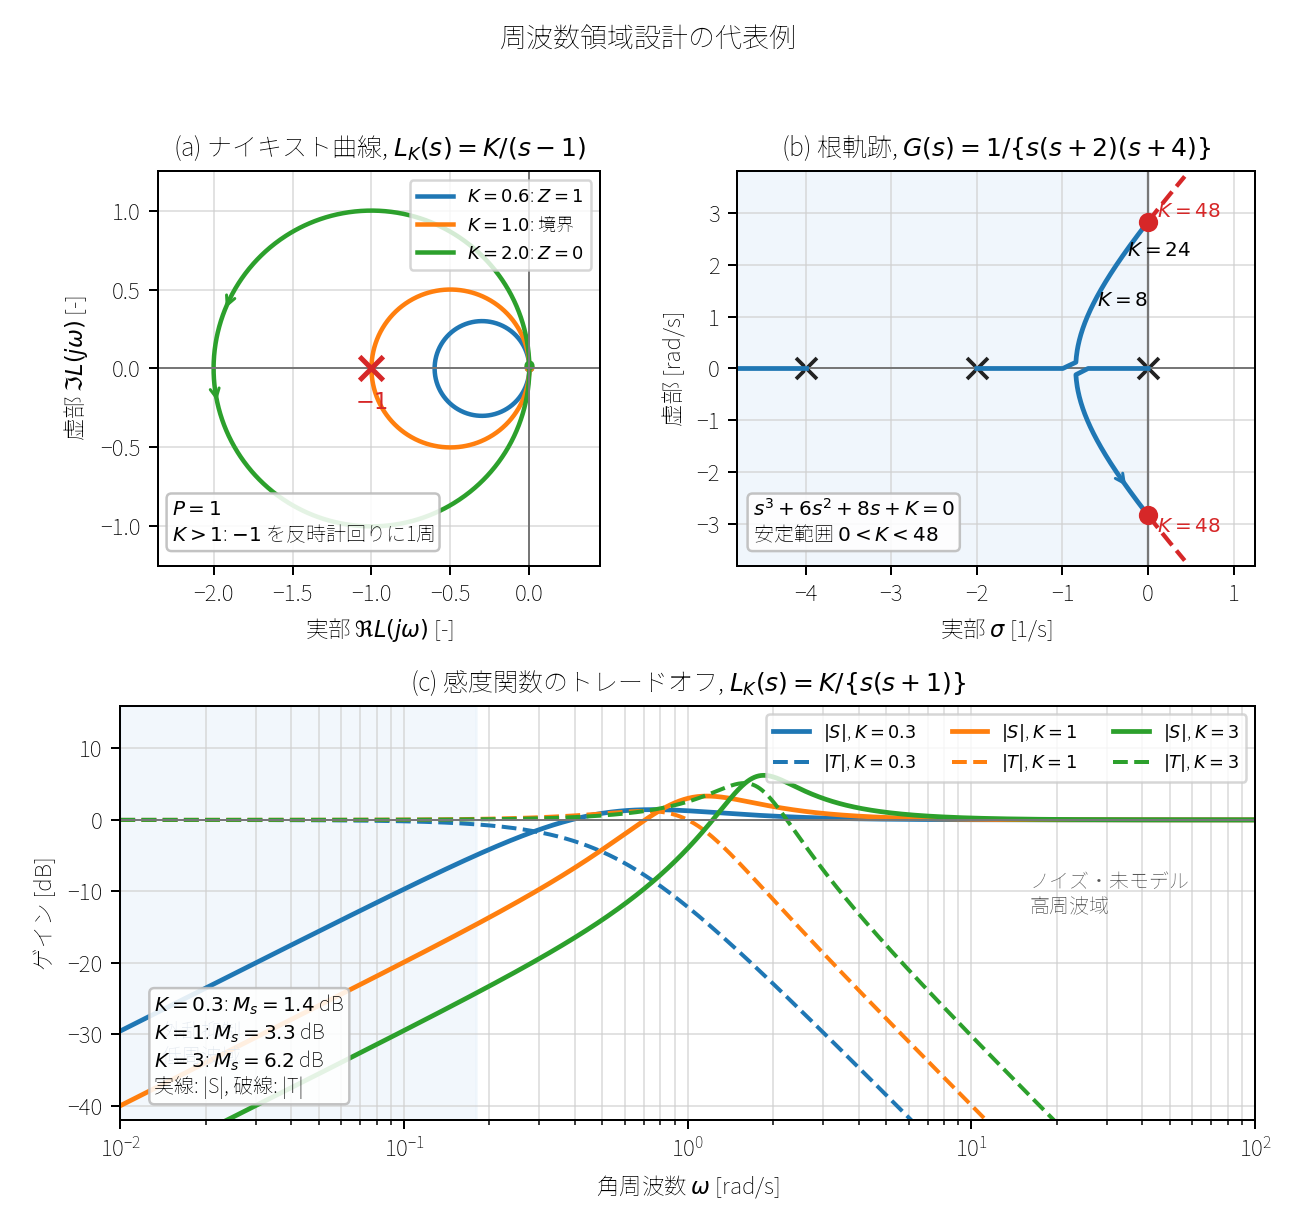
\includegraphics[width=0.96\linewidth,bb=0 0 1296 1224]{figures/frequency_design_examples.png}
\caption{ナイキスト線図、根軌跡、感度関数を同じ周波数設計の確認図として並べた例。上左は不安定開ループ極 $P=1$ を持つ $L_K(s)=K/(s-1)$ のゲイン変化で、$K>1$ だけが点 $-1$ を反時計回りに 1 回囲み閉ループが安定になる。上右は三次開ループ $G(s)=1/\{s(s+2)(s+4)\}$ の根軌跡で、$0<K<48$ が安定範囲、$K=48$ で虚軸を横切る。下は $L_K(s)=K/\{s(s+1)\}$ の $S$ と $T$ で、ゲインを上げるほど低周波の外乱抑制は強くなるが、感度ピークと相補感度の通過帯域が増える。}
\label{fig:frequency-design-examples}
\end{figure}

\begin{practice}[周波数設計図による安定性と感度の確認]
\wfig{frequency-design-examples} を用いる。上左で $K=0.6,1,2$ の各曲線について $N$、$P$、$Z$ を対応させ、上右で $K=48$ が安定限界になることを Routh 表の第一列と結びつけよ。最後に、下段の $K=0.3,1,3$ を比べ、低周波の $\abs{S}$、感度ピーク $M_s$、高周波側の $\abs{T}$ のどれが改善し、どれが悪化するかを一文ずつ述べよ。
\end{practice}

\subsubsection{むだ時間による位相損失}

むだ時間 $\tau_d$ を含む対象は、名目対象に $e^{-s\tau_d}$ が掛かった形で表される。周波数応答では
\begin{equation}
  \abs{e^{-j\omega\tau_d}}=1,\qquad
  \angle e^{-j\omega\tau_d}=-\omega\tau_d
\end{equation}
であり、ゲインを変えずに位相だけを遅らせる。ゲイン交差周波数 $\omega_{gc}$ の近くで安定余裕が決まる場合、位相余裕 $\phi_m$ をラジアンで表せば、むだ時間余裕の近似は
\begin{equation}
  \tau_{d,\max}\simeq\frac{\phi_m}{\omega_{gc}}
\end{equation}
である。交差周波数を高くして速い応答を得るほど、同じ位相余裕から得られるむだ時間余裕は短くなる。

むだ時間は乗法的不確かさとしても読める。むだ時間を無視した名目モデル $G(s)$ に対し、実対象が $G(s)e^{-s\tau_d}$ であるなら
\begin{equation}
  G(s)e^{-s\tau_d}
  =G(s)\{1+(e^{-s\tau_d}-1)\}
\end{equation}
である。したがって乗法誤差の大きさは
\begin{equation}
  \abs{e^{-j\omega\tau_d}-1}
  =2\abs{\sin\frac{\omega\tau_d}{2}}
  \simeq \omega\tau_d
  \qquad (\omega\tau_d\ll1)
\end{equation}
となる。高周波ほどむだ時間の相対誤差は大きくなるため、ロバスト安定条件 $\abs{W_mT}<1$ は高周波で $T$ を小さくする必要を与える。複数のゲイン交差や大きな共振ピークがある場合には、上の近似式だけでなくナイキスト線図または閉ループ極で確認する。

\begin{example}[一次対象の感度とむだ時間余裕]
一次対象
\begin{equation}
  G(s)=\frac{1}{s+1}
\end{equation}
を積分器 $C(s)=1/s$ で単位負帰還制御する。開ループは
\begin{equation}
  L(s)=\frac{1}{s(s+1)}
\end{equation}
であり、
\begin{equation}
  S(s)=\frac{s(s+1)}{s(s+1)+1},
  \qquad
  T(s)=\frac{1}{s(s+1)+1}
\end{equation}
である。低周波 $\omega=0.1\,\mathrm{rad/s}$ では $\abs{L(j\omega)}\simeq9.95$ なので、$\abs{S(j\omega)}$ はおよそ $0.1$、$\abs{T(j\omega)}$ はおよそ 1 である。目標値追従と低周波外乱抑制はよいが、同じ低周波に含まれる測定ノイズは出力へ通りやすい。

交差周波数は
\begin{equation}
  \frac{1}{\omega\sqrt{1+\omega^2}}=1
\end{equation}
から
\begin{equation}
  \omega_{gc}
  =\sqrt{\frac{\sqrt{5}-1}{2}}
  \simeq0.786\,\mathrm{rad/s}
\end{equation}
である。このとき開ループ位相は
\begin{equation}
  \angle L(j\omega_{gc})
  =-90^\circ-\tan^{-1}(0.786)
  \simeq-128.2^\circ
\end{equation}
なので、位相余裕は
\begin{equation}
  \phi_m\simeq51.8^\circ
  =0.904\,\mathrm{rad}
\end{equation}
である。むだ時間余裕の近似は
\begin{equation}
  \tau_{d,\max}\simeq\frac{0.904}{0.786}
  \simeq1.15\,\mathrm{s}
\end{equation}
となる。

交差周波数付近では感度が盛り上がる。たとえば $\omega=1\,\mathrm{rad/s}$ では
\begin{equation}
  L(j)=\frac{1}{j(1+j)}=-\frac{1}{2}-\frac{1}{2}j
\end{equation}
であるから
\begin{equation}
  \abs{S(j)}
  =\frac{1}{\abs{1+L(j)}}
  =\sqrt{2},\qquad
  \abs{T(j)}=1
\end{equation}
となる。低周波で $\abs{S}$ を下げた代償として、交差周波数付近に $\abs{S}>1$ の帯域が現れている。乗法誤差の上限がこの周波数帯で $\abs{W_m}\le0.3$ なら、少なくともこの点では $\abs{W_mT}\le0.3<1$ であり、乗法誤差だけから見ると余裕がある。一方、むだ時間が $1\,\mathrm{s}$ に近づくと交差周波数で約 $45^\circ$ の位相を失い、残りの位相余裕は小さい。応答を速くするためにゲインを上げれば $\omega_{gc}$ が上がり、同じむだ時間に対する位相損失はさらに大きくなる。
\end{example}

\subsection{外乱抑制とフィードフォワード}

外乱または目標値の変化が測定可能である場合、フィードフォワードを加えることで偏差伝達を低減できる。対象が $Y=G U+G_dD$ と書け、外乱 $D$ が測定可能であるなら
\begin{equation}
  U=C(R-Y)+F_dD
\end{equation}
とし、理想的には
\begin{equation}
  F_d(s)=-G(s)^{-1}G_d(s)
\end{equation}
を選ぶ。ただし $G^{-1}$ が不安定、非プロパー、または不確かな場合は直接実装できない。その場合には、低周波成分のみを補償する近似や入力制限を含む定式化を用いる。

目標値フィードフォワードも同じ考え方である。位置制御で目標軌道 $r(t)$ の速度や加速度が分かっていれば、必要な力を
\begin{equation}
  u_{ff}=m\ddot{r}+c\dot{r}+kr
\end{equation}
として与え、フィードバックでモデル誤差と外乱に起因する偏差を補償する。

\subsection{周波数領域を支える定理}

以下では、正弦波定常応答において伝達関数へ $s=j\omega$ を代入する根拠を示す。

\begin{theorem}[正弦波定常応答の定理]
安定な線形時不変系の伝達関数を $G(s)$ とする。入力 $u(t)=\operatorname{Re}\{Ue^{j\omega t}\}$ を加えると、過渡応答が消えた後の出力は
\begin{equation}
  y_{ss}(t)=\operatorname{Re}\{G(j\omega)Ue^{j\omega t}\}
\end{equation}
となる。
\end{theorem}

\begin{derivation}
複素指数入力 $u_c(t)=Ue^{j\omega t}$ を考える。線形時不変系では微分作用素 $\dd/\dd t$ に対して
\begin{equation}
  \frac{\dd}{\dd t}e^{j\omega t}=j\omega e^{j\omega t}
\end{equation}
である。たとえば微分方程式
\begin{equation}
  a_n y^{(n)}+\cdots+a_1\dot{y}+a_0y
  =b_m u^{(m)}+\cdots+b_0u
\end{equation}
に $y_c(t)=Ye^{j\omega t}$、$u_c(t)=Ue^{j\omega t}$ を代入する。$k$ 階微分は $(j\omega)^k$ 倍になるので
\begin{equation}
  \{a_n(j\omega)^n+\cdots+a_0\}Ye^{j\omega t}
  =\{b_m(j\omega)^m+
  \cdots+b_0\}Ue^{j\omega t}
\end{equation}
である。両辺を $e^{j\omega t}$ で割ると
\begin{equation}
  \frac{Y}{U}=\frac{b_m(j\omega)^m+\cdots+b_0}{a_n(j\omega)^n+\cdots+a_0}=G(j\omega)
\end{equation}
となる。したがって $Y=G(j\omega)U$ であり、実際の正弦波応答はその実部である。
\end{derivation}

\begin{formula}[ボード線図の積和変換]
複数の因子の積 $G(s)=G_1(s)G_2(s)$ に対して
\begin{equation}
  20\log_{10}\abs{G(j\omega)}
  =20\log_{10}\abs{G_1(j\omega)}+20\log_{10}\abs{G_2(j\omega)}
\end{equation}
である。また位相は
\begin{equation}
  \angle G(j\omega)=\angle G_1(j\omega)+\angle G_2(j\omega)
\end{equation}
である。
\end{formula}

\begin{derivation}
絶対値の性質 $\abs{ab}=\abs{a}\abs{b}$ と対数の性質 $\log(ab)=\log a+\log b$ より
\begin{align}
  20\log_{10}\abs{G_1G_2}
  &=20\log_{10}\{\abs{G_1}\abs{G_2}\}\\
  &=20\log_{10}\abs{G_1}+20\log_{10}\abs{G_2}.
\end{align}
複素数を $G_i=\abs{G_i}e^{j\phi_i}$ と書けば
\begin{equation}
  G_1G_2=\abs{G_1}\abs{G_2}e^{j(\phi_1+\phi_2)}
\end{equation}
なので、位相も和になる。
\end{derivation}

\begin{theorem}[ナイキスト安定判別]
単位負帰還系の開ループ $L(s)$ が虚軸上に極を持たず、$1+L(j\omega)\ne0$ であるとする。右半平面を時計回りに囲むナイキスト経路を用い、開ループ $L(s)$ の右半平面極の数を $P$、ナイキスト線図が点 $-1$ を時計回りに囲む回数を $N$ と数える。このとき閉ループ特性方程式 $1+L(s)=0$ の右半平面根の数 $Z$ は
\begin{equation}
  Z=N+P
\end{equation}
である。閉ループ安定性には $Z=0$ が必要十分である。
\end{theorem}

この定理は複素解析の偏角原理に基づく。反時計回りの囲みを正に数える流儀では符号が変わるため、ナイキスト判別を使うときは $N$ の符号規約を必ず明示する。ナイキスト線図は、閉ループ極の個数を周波数応答から決定するために用いられる。

\begin{formula}[根軌跡の角度条件と大きさ条件]
閉ループ特性方程式を $1+KG(s)=0$ とする。$K>0$ の根軌跡上の点 $s$ は
\begin{align}
  \angle G(s)&=(2\ell+1)\pi,\qquad \ell\in\mathbb{Z},\\
  K&=\frac{1}{\abs{G(s)}}
\end{align}
を満たす。
\end{formula}

\begin{derivation}
$1+KG(s)=0$ より
\begin{equation}
  KG(s)=-1
\end{equation}
である。右辺 $-1$ は大きさが 1、偏角が $(2\ell+1)\pi$ の複素数である。$K$ は正の実数なので偏角を変えない。したがって
\begin{equation}
  \angle G(s)=(2\ell+1)\pi
\end{equation}
でなければならない。また大きさを比べると
\begin{equation}
  K\abs{G(s)}=1
\end{equation}
だから
\begin{equation}
  K=1/\abs{G(s)}
\end{equation}
を得る。
\end{derivation}


\section{古典制御の設計法}

\subsection{ON-OFF 制御から比例・微分補正への設計動機}

白い床に引かれた黒線をライントレースロボットが進むとき、まず観察できる失敗は、線の中心を少し通り過ぎるたびに左右へ切り返し、蛇行しながら進むことである。線センサから得る横偏差を $e_y(t)\,[\mathrm{m}]$ とし、$e_y>0$ はロボット中心が線の左側にあることを表す。左右車輪の速度差指令を
\begin{equation}
  u_\Delta(t)=v_L(t)-v_R(t)\quad [\mathrm{m/s}]
\end{equation}
と定義し、$u_\Delta>0$ は左車輪を右車輪より速くして右へ旋回させる指令とする。この符号規約では、$e_y>0$ のとき右へ戻すために正の指令を出せばよい。

最初に実装しやすいのは、測定した偏差の符号だけで車輪指令を切り替える ON-OFF 制御である。
\begin{equation}
  u_\Delta(t)=
  \begin{cases}
    U_0, & e_y(t)>0,\\
    0, & e_y(t)=0,\\
    -U_0, & e_y(t)<0
  \end{cases}
  \qquad U_0\,[\mathrm{m/s}]>0
\end{equation}
線から左に外れたら右へ、右に外れたら左へ戻すため、方向は合っている。しかし指令の大きさは偏差 $1\,\mathrm{mm}$ でも $50\,\mathrm{mm}$ でも同じである。線の中心近くではセンサの微小な揺れだけで符号が入れ替わるので、指令は細かく反転し、機体の慣性があると横偏差は 0 の周りで持続的に振動する。

次の改善は、戻す量を横偏差の大きさに比例させることである。
\begin{equation}
  u_\Delta(t)=K_Pe_y(t),\qquad K_P\,[\mathrm{s}^{-1}]>0
\end{equation}
この P 制御では、線から大きく外れたときだけ大きく切り、中心に近づくほど指令が小さくなる。ON-OFF 制御の不連続な切替は消えるが、ロボットが中心を横切る瞬間にも横速度は残るため、比例項だけでは減速の情報が不足する。そこで横偏差の変化率も測り、中心へ近づく速度が大きいときに切り返しを弱める。
\begin{equation}
  u_\Delta(t)=K_Pe_y(t)+K_D\dot{e}_y(t),
  \qquad K_D\,[-]\geq0
\end{equation}
これが PD 制御であり、$K_D\dot{e}_y$ は横運動に対する減衰として働く。

この役割は小角度近似だけで確認できる。前進速度を $v_0\,[\mathrm{m/s}]$、車輪間隔を $b\,[\mathrm{m}]$、線に対する向きの偏差を $\theta(t)\,[\mathrm{rad}]$ とし、$\theta>0$ は左を向いている状態とする。すると
\begin{equation}
  \dot{e}_y=v_0\theta,\qquad
  \dot{\theta}=-\frac{1}{b}u_\Delta
\end{equation}
である。P 制御を代入すると
\begin{equation}
  \ddot{e}_y+\frac{v_0K_P}{b}e_y=0
\end{equation}
となり、減衰項を持たない二次系になる。したがって比例ゲインは中心へ戻す強さを作るが、単独では横切った後の振動を消さない。PD 制御なら
\begin{equation}
  \ddot{e}_y+\frac{v_0K_D}{b}\dot{e}_y
  +\frac{v_0K_P}{b}e_y=0
\end{equation}
となり、$\dot{e}_y$ の係数が正なら横運動のエネルギーが減る。

\wfig{line-following-feedback-bridge} は、この計算を同じ初期横偏差 $e_y(0)=0.06\,\mathrm{m}$ から比べたものである。$v_0=0.35\,\mathrm{m/s}$、$b=0.12\,\mathrm{m}$、ON-OFF の $U_0=0.12\,\mathrm{m/s}$、P/PD の $K_P=1.45\,\mathrm{s}^{-1}$、$K_D=0.75$ とした。ON-OFF では中心付近の $6\,\mathrm{mm}$ の測定揺れだけで車輪指令が反転し、偏差の振動も残る。P 制御では指令は連続になるが、上式の通り減衰がないため振動の振幅はほとんど減らない。PD 制御では同じ $K_P$ でも $\dot{e}_y$ に比例した項が横切り速度を打ち消し、数秒以内に偏差と車輪指令の両方が 0 へ近づく。

\begin{figure}[tbp]
\centering
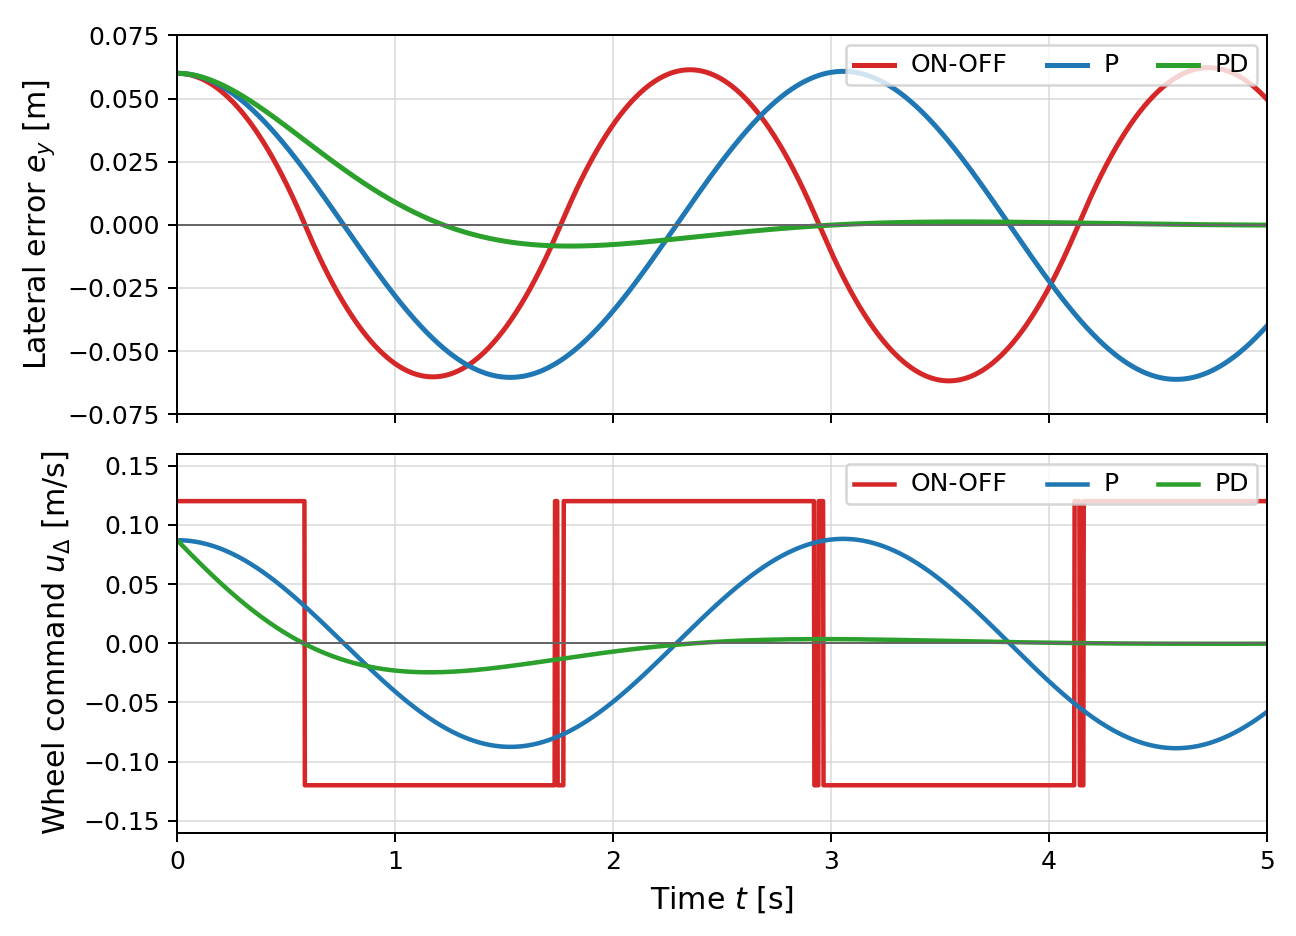
\includegraphics[width=0.96\linewidth,bb=0 0 1296 936]{figures/line_following_feedback_bridge.png}
\caption{ライントレースロボットの横偏差に対する ON-OFF、P、PD 制御の比較。上段は横偏差 $e_y$、下段は左右車輪速度差指令 $u_\Delta=v_L-v_R$ を示す。ON-OFF 制御は符号切替により中心付近で指令が反転し、P 制御は連続指令に変わるが減衰を持たず、PD 制御は横偏差の変化率を使って振動を減らす。}
\label{fig:line-following-feedback-bridge}
\end{figure}

\subsection{古典制御の設計基準と評価指標}

周波数領域の指標を時間応答・安定判別・補償器設計へ接続し、古典制御を設計手順として整理する。

ここまでで、一次遅れ、二次遅れ、ラプラス変換、伝達関数、周波数応答を導入した。古典制御は、仕様、安定判別、補償器構成、実装上の制約を結び付ける設計体系である。本節では、標準的な項目を時間応答、根軌跡、周波数応答、感度関数の順に整理する。

古典制御で反復して評価する設計基準は四つである。第一に閉ループの漸近安定性、第二に目標値応答の速さと振動の小ささ、第三に外乱およびモデル誤差に対するロバスト性、第四にアクチュエータが要求入力を実現できることである。これらを時間応答、根軌跡、周波数応答、感度関数で相補的に評価する。

\subsection{二次系のステップ応答を最後まで解く}

二次標準形
\begin{equation}
  G(s)=\frac{\omega_n^2}{s^2+2\zeta\omega_n s+\omega_n^2}
\end{equation}
に単位ステップ入力 $R(s)=1/s$ を入れる。出力は
\begin{equation}
  Y(s)=G(s)R(s)=
  \frac{\omega_n^2}{s(s^2+2\zeta\omega_n s+\omega_n^2)}
  \label{eq:second-order-step-laplace}
\end{equation}
である。$0<\zeta<1$ の不足減衰の場合をまず扱う。分母の二次式を平方完成する。
\begin{align}
  s^2+2\zeta\omega_n s+\omega_n^2
  &=(s+\zeta\omega_n)^2+\omega_n^2-\zeta^2\omega_n^2\\
  &=(s+\zeta\omega_n)^2+
    \omega_n^2(1-
    \zeta^2).
\end{align}
ここで
\begin{equation}
  \omega_d=\omega_n\sqrt{1-\zeta^2}
\end{equation}
を減衰固有角周波数という。

\begin{derivation}
\weq{second-order-step-laplace} を
\begin{equation}
  Y(s)=\frac{1}{s}-
  \frac{s+2\zeta\omega_n}{s^2+2\zeta\omega_n s+\omega_n^2}
\end{equation}
と分ける。右辺を通分すると
\begin{align}
  \frac{1}{s}-\frac{s+2\zeta\omega_n}{s^2+2\zeta\omega_n s+\omega_n^2}
  &=\frac{s^2+2\zeta\omega_n s+\omega_n^2-s(s+2\zeta\omega_n)}{s(s^2+2\zeta\omega_n s+\omega_n^2)}\\
  &=\frac{\omega_n^2}{s(s^2+2\zeta\omega_n s+\omega_n^2)}
\end{align}
となり、確かに元の $Y(s)$ と一致する。さらに
\begin{equation}
  s+2\zeta\omega_n=(s+\zeta\omega_n)+\zeta\omega_n
\end{equation}
なので
\begin{align}
  Y(s)
  &=\frac{1}{s}-
  \frac{s+\zeta\omega_n}{(s+\zeta\omega_n)^2+
  \omega_d^2}
  -\frac{\zeta\omega_n}{(s+\zeta\omega_n)^2+
  \omega_d^2}.
\end{align}
ラプラス逆変換の公式
\begin{align}
  \mathcal{L}^{-1}\left\{\frac{s+a}{(s+a)^2+b^2}\right\}&=e^{-at}\cos bt,\\
  \mathcal{L}^{-1}\left\{\frac{b}{(s+a)^2+b^2}\right\}&=e^{-at}\sin bt
\end{align}
より、
\begin{equation}
  y(t)=1-e^{-\zeta\omega_n t}\cos\omega_d t
  -\frac{\zeta\omega_n}{\omega_d}e^{-\zeta\omega_n t}\sin\omega_d t.
\end{equation}
$\omega_d=\omega_n\sqrt{1-\zeta^2}$ を代入すると
\begin{equation}
  y(t)=1-e^{-\zeta\omega_n t}
  \left(\cos\omega_d t+\frac{\zeta}{\sqrt{1-\zeta^2}}\sin\omega_d t\right)
  \label{eq:underdamped-step-response}
\end{equation}
である。
\end{derivation}

\subsubsection{ピーク時刻とオーバーシュート}

ピークは $\dot{y}(t)=0$ で決まる。ここでは、位相を無理にまとめず、\weq{underdamped-step-response} を直接微分して最初のピーク時刻と行き過ぎ量を求める。

\begin{derivation}
\weq{underdamped-step-response} の括弧内を
\begin{equation}
  q(t)=\cos\omega_d t+
  \frac{\zeta}{\sqrt{1-\zeta^2}}\sin\omega_d t
\end{equation}
とおくと、$y(t)=1-e^{-\zeta\omega_n t}q(t)$ である。したがって
\begin{align}
  \dot{y}(t)
  &=-\frac{d}{dt}\left\{e^{-\zeta\omega_n t}q(t)\right\}\\
  &=e^{-\zeta\omega_n t}
  \left\{\zeta\omega_n q(t)-\dot{q}(t)\right\}.
\end{align}
ここで
\begin{equation}
  \dot{q}(t)=
  -\omega_d\sin\omega_d t+
  \frac{\zeta\omega_d}{\sqrt{1-\zeta^2}}\cos\omega_d t
\end{equation}
なので、
\begin{align}
  \dot{y}(t)
  &=e^{-\zeta\omega_n t}
  \left[
  \left(\zeta\omega_n-
  \frac{\zeta\omega_d}{\sqrt{1-\zeta^2}}\right)\cos\omega_d t
  +\left(
  \frac{\zeta^2\omega_n}{\sqrt{1-\zeta^2}}+\omega_d
  \right)\sin\omega_d t
  \right].
\end{align}
$\omega_d=\omega_n\sqrt{1-\zeta^2}$ より、余弦の係数は
\begin{equation}
  \zeta\omega_n-
  \frac{\zeta\omega_d}{\sqrt{1-\zeta^2}}
  =\zeta\omega_n-\zeta\omega_n=0
\end{equation}
と消える。また、正弦の係数は
\begin{align}
  \frac{\zeta^2\omega_n}{\sqrt{1-\zeta^2}}+\omega_d
  &=
  \frac{\zeta^2\omega_n}{\sqrt{1-\zeta^2}}
  +\omega_n\sqrt{1-\zeta^2}\\
  &=\frac{\omega_n}{\sqrt{1-\zeta^2}}
\end{align}
である。したがって
\begin{equation}
  \dot{y}(t)=
  \frac{\omega_n}{\sqrt{1-\zeta^2}}
  e^{-\zeta\omega_n t}\sin\omega_d t
\end{equation}
となる。指数関数と係数は正なので、$\dot{y}(t)=0$ は
\begin{equation}
  \sin\omega_d t=0
\end{equation}
で決まる。$t>0$ で最初にこれを満たす時刻は
\begin{equation}
  t_p=\frac{\pi}{\omega_d}
\end{equation}
であり、$0<t<\pi/\omega_d$ では $\sin\omega_d t>0$、$\pi/\omega_d<t<2\pi/\omega_d$ では $\sin\omega_d t<0$ なので、これは最初のピークである。

この時刻では
\begin{equation}
  \cos\omega_d t_p=\cos\pi=-1,
  \qquad
  \sin\omega_d t_p=\sin\pi=0
\end{equation}
だから、
\begin{align}
  y(t_p)
  &=1-e^{-\zeta\omega_n t_p}(-1)\\
  &=1+e^{-\zeta\omega_n t_p}.
\end{align}
最終値 1 からの行き過ぎ量は
\begin{align}
  M_p&=y(t_p)-1\\
  &=\exp(-\zeta\omega_n t_p)\\
  &=\exp\left(-\zeta\omega_n\frac{\pi}{\omega_d}\right)\\
  &=\exp\left(-\frac{\pi\zeta}{\sqrt{1-\zeta^2}}\right).
\end{align}
百分率で表すと $100M_p\%$ である。
\end{derivation}

整定時間の目安も式から出る。振動部分の包絡線は $e^{-\zeta\omega_n t}$ なので、2\% 整定なら
\begin{align}
  e^{-\zeta\omega_n t}&=0.02,\\
  -\zeta\omega_n t&=\log 0.02,\\
  t&=\frac{-\log 0.02}{\zeta\omega_n}\simeq
  \frac{3.9}{\zeta\omega_n}.
\end{align}
このため実務上は
\begin{equation}
  T_s\simeq\frac{4}{\zeta\omega_n}
\end{equation}
を使う。これは丸暗記の経験則ではなく、指数包絡線が 2\% まで下がる時刻の近似である。

\subsection{逆ラプラス変換と極零点の解釈}

古典制御では、$s$ 領域の式を時間応答へ戻す計算を何度も行う。基本は部分分数分解である。

\begin{formula}[単純極の部分分数分解]
相異なる極 $p_1,\ldots,p_n$ を持つ真にプロパーな伝達関数
\begin{equation}
  F(s)=\frac{N(s)}{(s-p_1)(s-p_2)\cdots(s-p_n)}
\end{equation}
は
\begin{equation}
  F(s)=\sum_{i=1}^{n}\frac{r_i}{s-p_i}
\end{equation}
と書ける。係数 $r_i$ を留数と呼び、
\begin{equation}
  r_i=\lim_{s\to p_i}(s-p_i)F(s)
\end{equation}
で求まる。
\end{formula}

\begin{derivation}
例として
\begin{equation}
  F(s)=\frac{3s+5}{(s+1)(s+4)}
\end{equation}
を考える。部分分数分解を
\begin{equation}
  F(s)=\frac{A}{s+1}+\frac{B}{s+4}
\end{equation}
と置く。通分すると
\begin{equation}
  3s+5=A(s+4)+B(s+1)
\end{equation}
である。$s=-1$ を代入すると
\begin{equation}
  -3+5=A(3)+B(0)
\end{equation}
なので $A=2/3$。$s=-4$ を代入すると
\begin{equation}
  -12+5=A(0)+B(-3)
\end{equation}
なので $B=7/3$。したがって
\begin{equation}
  F(s)=\frac{2/3}{s+1}+\frac{7/3}{s+4}
\end{equation}
であり、逆ラプラス変換は
\begin{equation}
  f(t)=\frac{2}{3}e^{-t}+\frac{7}{3}e^{-4t}
\end{equation}
である。
\end{derivation}

複素共役極 $-\sigma\pm j\omega$ は、時間領域では
\begin{equation}
  e^{-\sigma t}\cos\omega t,
  \qquad
  e^{-\sigma t}\sin\omega t
\end{equation}
の組として現れる。したがって、実部は減衰、虚部は振動を決める。零点は指数成分そのものを新しく作るのではなく、それぞれの指数成分の重みを変える。右半平面零点があると、最終的に正へ動く応答が初めに逆向きへ動くことがある。

\subsection{定常偏差と最終値の定理}

PD 制御は行き過ぎを抑え、振動を減らす。しかし、応答が静かになったあとにも目標値から一定量だけずれていれば、実機では制御できているとは言いにくい。たとえば小さな水槽の水位 $y$ [m] をポンプ入力 $u$ [\%] で保つとき、細い漏れがあると、目標水位 $r$ [m] に止まって見えても常に補給入力が必要になる。偏差 $e=r-y$ [m] に比例する P 制御と、偏差の変化率に比例する D 制御だけでは、定常状態で $\dot{e}=0$ となるため微分項は入力を出さない。必要な補給入力を比例項だけで作るには、$u_\infty=k_\mathrm{P}e_\infty$ となる非零の偏差が残る。

この残り偏差を測定量として見ると、比例ゲインを大きくすれば小さくはなるが、一定外乱がある限り 0 にはならない。積分動作は、この「小さいが消えない偏差」を時間方向に集める状態
\begin{equation}
  \eta(t)=\int_0^t e(\tau)\,d\tau,
  \qquad
  \dot{\eta}=e
\end{equation}
を制御器の内部に持たせる考えである。水位偏差 $e$ の単位が [m] なら、積分状態 $\eta$ の単位は [m\,s] である。入力を
\begin{equation}
  u=k_\mathrm{P}e+k_\mathrm{I}\eta
\end{equation}
とすれば、$k_\mathrm{I}$ の単位は [\%/(m\,s)] であり、偏差が正のあいだ $\eta$ が増え続け、漏れを打ち消すための一定入力を作る。最終的に $e=0$ になれば $\dot{\eta}=0$ となり、積分状態はそこで止まって、必要な補給入力だけを保持する。

\begin{theorem}[最終値の定理]
$sF(s)$ のすべての極が左半平面にあるとき、
\begin{equation}
  \lim_{t\to\infty}f(t)=\lim_{s\to0}sF(s)
\end{equation}
が成り立つ。
\end{theorem}

負帰還で開ループ $L(s)=C(s)G(s)$ とすると、偏差は
\begin{align}
  E(s)&=R(s)-Y(s),\\
  Y(s)&=L(s)E(s).
\end{align}
よって
\begin{align}
  E(s)&=R(s)-L(s)E(s),\\
  \{1+L(s)\}E(s)&=R(s),\\
  E(s)&=\frac{1}{1+L(s)}R(s)=S(s)R(s).
\end{align}
単位ステップ $R(s)=1/s$ に対する定常偏差は、最終値の定理より
\begin{align}
  e_\infty&=\lim_{s\to0}sE(s)\\
  &=\lim_{s\to0}s\frac{1}{1+L(s)}\frac{1}{s}\\
  &=\frac{1}{1+L(0)}.
\end{align}
この計算は、閉ループが安定であり、$sE(s)$ の極が左半平面にある場合にだけ定常値を表す。型 0 のループでは $L(0)$ が有限なので、一定目標や一定外乱に対する残り偏差は有限値として残る。一方、積分器を一つ入れると低周波で $L(s)=\tilde{L}(s)/s$ となり、$\tilde{L}(0)$ が有限正で閉ループが安定なら
\begin{align}
  e_\infty
  &=\lim_{s\to0}\frac{1}{1+\tilde{L}(s)/s}\\
  &=\lim_{s\to0}\frac{s}{s+\tilde{L}(s)}=0
\end{align}
である。これは、積分状態 $\eta$ が漏れや重力分などの一定バイアス入力を保持し、偏差そのものは 0 に近づけられる、という水槽の観察と同じ内容である。

\begin{center}
\begin{tabular}{lll}
\hline
構成 & 低周波の開ループ & 単位ステップ定常偏差 \\
\hline
型 0 & $L(0)=K_p<\infty$ & $1/(1+K_p)$ \\
積分器 1 個 & $L(s)=\tilde{L}(s)/s,\ \tilde{L}(0)>0$ & $0$ \\
\hline
\end{tabular}
\end{center}

\begin{definition}[型と誤差定数]
開ループ $L(s)$ が原点に持つ極の個数を系の型という。位置、速度、加速度誤差定数を
\begin{align}
  K_p&=\lim_{s\to0}L(s),\\
  K_v&=\lim_{s\to0}sL(s),\\
  K_a&=\lim_{s\to0}s^2L(s)
\end{align}
と定義する。
\end{definition}

ステップ、ランプ、放物線入力に対する定常偏差は、閉ループが安定であるという前提のもとで
\begin{align}
  e_{step}&=\frac{1}{1+K_p},\\
  e_{ramp}&=\frac{1}{K_v},\\
  e_{parabolic}&=\frac{1}{K_a}
\end{align}
となる。積分器 $1/s$ を制御器に入れると原点極が一つ増えるため、ステップ偏差を 0 にできる。ただし積分状態は過去の偏差を蓄えるので、むやみに $k_\mathrm{I}$ を大きくすると低周波の補正は強くなる一方で位相遅れも増え、安定余裕は悪くなりやすい。

\subsection{ブロック線図の全経路}

閉ループ評価は目標値応答だけでは不十分である。入力外乱、出力外乱、測定ノイズ、制御入力も同時に評価する必要がある。図\ref{fig:closed-loop-signal-paths} に、同じ負帰還ループでこれらの信号が入る位置を示す。ここでは単位帰還の SISO 系を考え、開ループを $L=CG$、感度を $S=1/(1+L)$、相補感度を $T=L/(1+L)$ とする。

\begin{figure}[tbp]
\centering
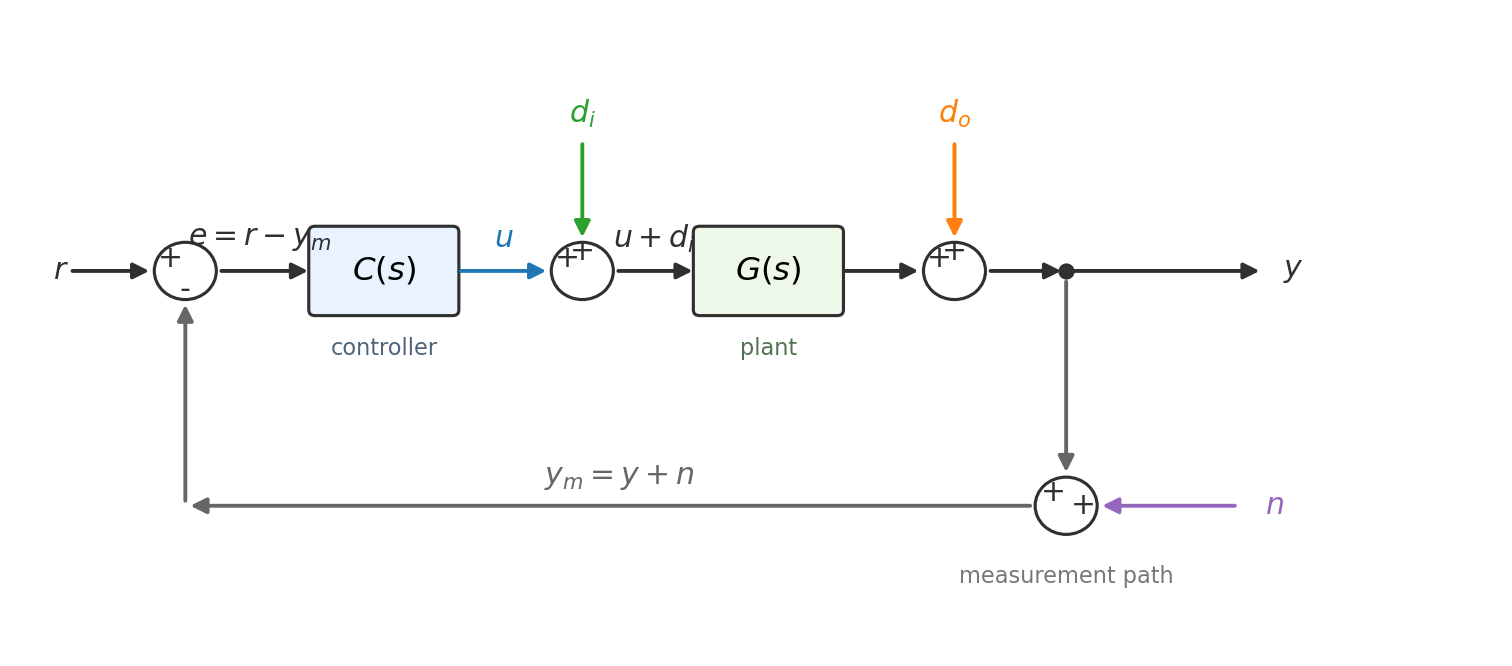
\includegraphics[width=0.96\linewidth,bb=0 0 1512 666]{figures/closed_loop_signal_paths.png}
\caption{目標値 $r$、制御器 $C$、制御対象 $G$、入力外乱 $d_i$、出力外乱 $d_o$、測定ノイズ $n$、制御器出力 $u$、出力 $y$ を含む閉ループの信号経路。入力外乱 $d_i$ は対象入力側に加わるため $GS$ の経路で $y$ を動かし、制御器出力 $u$ にも反作用を生む。出力外乱 $d_o$ は対象後段で $y$ に直接加わり、感度 $S$ で抑えられる。測定ノイズ $n$ は実出力を直接変えず、測定値 $y_m=y+n$ を通じて $-T$ と $-CS$ の経路に入る。$u$ を同時に確認しないと、出力偏差が小さい条件でもアクチュエータ飽和やノイズ増幅を検出できない。}
\label{fig:closed-loop-signal-paths}
\end{figure}

図の符号規約では、入力外乱 $d_i$ が対象入力に加わり、出力外乱 $d_o$ が対象出力の後で加わり、測定ノイズ $n$ は帰還される測定値 $y_m=y+n$ にだけ入る。したがって、すべての入力点を同時に残すと
\begin{align}
  y&=G(u+d_i)+d_o,\\
  u&=C\{r-(y+n)\}
\end{align}
である。代入して整理すると
\begin{align}
  y&=G\{C(r-y-n)+d_i\}+d_o,\\
  y+GCy&=GCr+Gd_i+d_o-GCn,\\
  (1+L)y&=Lr+Gd_i+d_o-Ln.
\end{align}
したがって
\begin{equation}
  y=Tr+GSd_i+Sd_o-Tn.
\end{equation}
目標値だけを入れれば $y=Tr$、入力外乱だけを入れれば $y=GSd_i$、出力外乱だけを入れれば $y=Sd_o$、測定ノイズだけを入れれば $y=-Tn$ である。入力外乱は対象 $G$ を通ってから感度 $S$ で抑えられ、出力外乱は対象の後で加わるため $G$ を通らない。測定ノイズは出力そのものを動かす外力ではないが、帰還信号を誤らせるため相補感度 $T$ を通じて出力に現れる。

制御器出力は
\begin{align}
  u&=C(r-y-n)\\
  &=C\{r-(Tr+GSd_i+Sd_o-Tn)-n\}\\
  &=CSr-CGSd_i-CSd_o-CSn
\end{align}
である。$u$ の式には、外乱を打ち消そうとして制御器がどれだけ大きな指令を出すかが現れる。低周波で $S$ が小さくても、$C$ や $CGS$ が大きい帯域では、外乱補償や測定ノイズのために $u$ が先に飽和することがある。したがって閉ループ設計では、出力 $y$ の小ささだけでなく、制御器出力 $u$、飽和余裕、ノイズ帯域での増幅を同じ条件で確認する。

\subsection{古典補償器の設計}

補償器設計は、要求仕様を開ループ $L(s)=C(s)G(s)$ の形へ翻訳する作業である。位相余裕を増やしたいなら進み補償、低周波ゲインを増やして定常偏差を減らしたいなら遅れ補償、両方必要なら遅れ進み補償を使う。

\begin{definition}[進み補償]
\begin{equation}
  C_{lead}(s)=K\frac{1+Ts}{1+\alpha Ts},
  \qquad 0<\alpha<1
\end{equation}
を進み補償という。零点が極より低い周波数にあるため、ある周波数帯で正の位相を加える。
\end{definition}

最大位相進みは
\begin{equation}
  \phi_{max}=\sin^{-1}\frac{1-\alpha}{1+\alpha}
\end{equation}
であり、その周波数は
\begin{equation}
  \omega_m=\frac{1}{T\sqrt{\alpha}}
\end{equation}
である。設計では、必要な位相余裕の不足分に安全余裕を足し、$\alpha$ を決め、望むゲイン交差周波数を $\omega_m$ 付近へ置くように $T$ を決める。

\begin{definition}[遅れ補償]
\begin{equation}
  C_{lag}(s)=K\frac{1+Ts}{1+\beta Ts},
  \qquad \beta>1
\end{equation}
を遅れ補償という。低周波ゲインを相対的に上げ、定常偏差を小さくするために使う。
\end{definition}

遅れ補償は位相を少し遅らせるので、ゲイン交差周波数の近くに置くと安定余裕を悪くする。したがって、折点はゲイン交差周波数より十分低く置き、低周波の精度改善を主目的にする。

\subsection{フィードフォワード、カスケード制御、外乱オブザーバ}

閉ループ制御は、測定した偏差を使って未知の誤差を修正する構造である。一方、目標値の変化、加速度指令、荷重、流量、周囲温度のように、制御対象へ加わる信号の一部があらかじめ分かっている場合がある。この既知情報を偏差が現れる前に操作量へ入れる方法をフィードフォワード制御という。フィードフォワードはフィードバックの代わりではない。モデルが正しい範囲で必要入力を先に出し、モデル誤差、未知外乱、初期値ずれをフィードバックで補正する構成である。

\subsubsection{既知目標値と既知外乱からのフィードフォワード}

まず、対象を
\begin{equation}
  y=G(s)u+G_d(s)d
\end{equation}
で表す。$u$ は操作量、$d$ は外乱、$G_d$ は外乱から出力までの伝達関数である。外乱 $d$ が測定または予測でき、その測定値を $d_m$ とする。フィードバック制御器を $C(s)$、外乱フィードフォワードを $F_d(s)$ として
\begin{equation}
  u=C(s)(r-y)+F_d(s)d_m
\end{equation}
を入れる。$d_m=d$ と仮定して代入すると
\begin{align}
  y&=G\{C(r-y)+F_d d\}+G_d d,\\
  (1+GC)y&=GCr+(GF_d+G_d)d,
\end{align}
したがって
\begin{equation}
  y=\frac{GC}{1+GC}r+
  \frac{GF_d+G_d}{1+GC}d
\end{equation}
である。名目モデル $G_n,G_{d,n}$ が正しく、$G_n^{-1}G_{d,n}$ が安定でプロパーに実装できるなら
\begin{equation}
  F_d(s)=-G_n(s)^{-1}G_{d,n}(s)
\end{equation}
と選ぶことで、名目上は $GF_d+G_d=0$ となり、外乱項が消える。外乱が対象入力にそのまま加わる入力外乱では $G_d=G$ なので、理想的な補償は単に $F_d=-1$ である。これは、既知の入力外乱と反対向きの入力を先に加えるという意味である。

目標値に対しても同じ考え方を使える。名目対象 $G_n$ に対し、望ましい目標値応答を安定でプロパーな伝達関数 $M(s)$ として与える。開ループの必要入力を
\begin{equation}
  u_{ff}=F_r(s)r,
  \qquad
  F_r(s)=G_n(s)^{-1}M(s)
\end{equation}
とすれば、名目上は $y=M r$ になる。ただし、この式がそのまま使えるとは限らない。$G_n$ に右半平面零点やむだ時間があると、安定な因果系として正確な逆系を作れない。相対次数が大きい対象では $G_n^{-1}M$ がプロパーでなくなることもある。このため、実装では $M$ を十分遅くし、必要なら低域通過フィルタを加え、入力飽和を越えない範囲で近似逆を使う。

フィードフォワード設計で明示すべき仮定は三つである。第一に、既知信号 $r$ または $d_m$ が制御計算に間に合う時点で利用でき、正しい単位と符号を持つこと。第二に、名目モデルの逆を使う周波数帯で、零点、むだ時間、未モデル化高周波動特性が無視できること。第三に、フィードフォワード入力を加えてもアクチュエータが飽和しないことである。これらが崩れると、偏差が小さくなるどころか、誤った先回り入力によってフィードバックが補正すべき誤差を増やしてしまう。

\subsubsection{二自由度構造としての解釈}

一自由度の負帰還では、同じ制御器 $C$ が目標値追従と外乱抑制の両方を決める。これに対し、目標値から入力への経路と、測定値から入力への経路を分けて
\begin{equation}
  u=C_r(s)r-C_y(s)y
\end{equation}
と書く構造を二自由度制御構造という。対象入力に外乱 $d_i$ が加わる場合、
\begin{align}
  y&=G(u+d_i),\\
  u&=C_r r-C_y y
\end{align}
であるから
\begin{align}
  y&=G(C_r r-C_y y+d_i),\\
  (1+GC_y)y&=GC_r r+Gd_i.
\end{align}
したがって
\begin{equation}
  y=\frac{GC_r}{1+GC_y}r+
  \frac{G}{1+GC_y}d_i
\end{equation}
となる。分母 $1+GC_y$ は、閉ループ極、安定余裕、外乱抑制、測定ノイズの入り方を決める。一方、$C_r$ は主に目標値から出力までの分子を変える。つまり、$C_y$ でロバスト性と外乱抑制を確保し、$C_r$ または $F_r=C_r-C_y$ で目標値応答を整える、という役割分担ができる。

後で扱う二自由度 PID は、この構造の実装例である。比例項と微分項に目標値重みを入れると、測定値側のフィードバックを保ったまま、目標値ステップに対する比例キックや微分キックを弱められる。ただし、二自由度化しても閉ループ安定性の基本は $1+GC_y$ に残る。目標値経路だけを滑らかにしても、出力外乱やモデル誤差への性質が自動的に改善するわけではない。

\subsubsection{カスケード制御と帯域分離}

一つの制御対象の中に、速く測れる内部量と、遅く制御したい外部量がある場合は、制御ループを内側と外側に分ける。これをカスケード制御という。入力 $u$ から内部量 $z$ までの伝達関数を $G_i$、内部量 $z$ から出力 $y$ までの伝達関数を $G_o$ とする。
\begin{equation}
  z=G_i(u+d_i),
  \qquad
  y=G_o z
\end{equation}
内側制御器 $C_i$ が $z$ を目標値 $z_r$ に追従させ、外側制御器 $C_o$ が $z_r$ を作る。
\begin{equation}
  u=C_i(z_r-z),
  \qquad
  z_r=C_o(r-y)
\end{equation}
内側閉ループの感度と相補感度を
\begin{equation}
  S_i=\frac{1}{1+G_iC_i},
  \qquad
  T_i=\frac{G_iC_i}{1+G_iC_i}
\end{equation}
とおくと、
\begin{align}
  z&=T_i z_r+G_iS_i d_i,\\
  y&=G_oT_i z_r+G_oG_iS_i d_i.
\end{align}
外側ループに対する等価制御対象は $G_oT_i$ である。内側ループの帯域幅を $\omega_{b,i}$、外側ループの帯域幅を $\omega_{b,o}$ とすると、外側設計の周波数範囲で
\begin{equation}
  T_i(j\omega)\simeq 1,
  \qquad
  \angle T_i(j\omega)\simeq 0
  \quad
  (0\leq\omega\leq \omega_{b,o})
\end{equation}
となるように、通常は
\begin{equation}
  \omega_{b,i}\geq 3\omega_{b,o}
\end{equation}
を最低条件とし、余裕があれば $5$ 倍から $10$ 倍程度の分離を取る。内側ループが十分速ければ、外側ループは $z$ がほぼ指令通りに動くものとして設計できる。また、$G_iS_i d_i$ が小さくなるため、入力側や内部側の外乱は外側へ伝わる前に抑えられる。

カスケード制御が有効であるためには、内部量 $z$ を測定できること、内側アクチュエータが外側の要求より速く動けること、内側ループ単独で安定余裕を持つことが必要である。内側に強いノイズ、量子化、むだ時間がある場合、帯域を上げるほど外側へ位相遅れとノイズが入る。さらに、内側が飽和すると外側制御器は「内部量が追従している」という前提を失うため、外側の積分器にもアンチワインドアップを入れる必要がある。

\subsubsection{外乱オブザーバの基本構成}

外乱が測れない場合でも、名目モデルを使って「入力から予測される出力」と「実際の出力」の差から外乱を推定できることがある。この考え方を外乱オブザーバという。ここでは、外乱 $d$ が対象入力に加わる
\begin{equation}
  y=P(s)\{u+d\}
\end{equation}
という形を考える。名目モデルを $P_n(s)$ とし、低域通過フィルタを $Q(s)$ とする。外乱推定値を
\begin{equation}
  \hat{d}=Q(s)\{P_n(s)^{-1}y-u\}
\end{equation}
で作り、補償後の入力を
\begin{equation}
  u=u_0-\hat{d}
\end{equation}
とする。もし $P=P_n$ なら、
\begin{align}
  P_n^{-1}y-u
  &=P_n^{-1}P_n(u+d)-u\\
  &=d
\end{align}
なので
\begin{equation}
  \hat{d}=Qd
\end{equation}
である。したがって対象へ入る合計入力は
\begin{equation}
  u+d=u_0+(1-Q)d
\end{equation}
となる。低周波で $Q(j\omega)\simeq 1$ なら、その帯域の外乱はほぼ打ち消される。高周波で $Q(j\omega)\simeq 0$ とすれば、センサノイズや未モデル化動特性を逆モデルで増幅することを避けられる。

外乱オブザーバでは $Q$ フィルタの選択が中心である。$Q(0)=1$ として定常外乱を推定し、遮断周波数を上げるほど外乱抑制帯域は広がる。しかし $P_n^{-1}$ は高周波で大きなゲインを持ちやすく、相対次数のためにプロパーでないこともある。このため、$Q P_n^{-1}$ がプロパーで安定になるように、$Q$ の次数を十分高くする。名目モデルが右半平面零点やむだ時間を持つ場合、厳密な安定逆は作れないので、最小位相部分だけを反転する近似逆を使う。さらに、外乱オブザーバはモデル誤差を外乱として扱うため、$Q$ の帯域を未モデル化共振やサンプリング周波数に近づけすぎると、かえって閉ループを不安定化する。

\begin{example}[DC モータ速度制御における構成例]
DC モータの角速度を $\omega$、電流を $i$、電圧を $v$、負荷トルクを $\tau_L$ とする。単純化したモデルは
\begin{align}
  J\dot{\omega}+b\omega&=K_t i-\tau_L,\\
  L\dot{i}+Ri&=v-K_e\omega
\end{align}
である。電流は速度より速く測定・制御できることが多いため、内側に電流ループ、外側に速度ループを置く。内側電流ループの帯域を速度ループの少なくとも数倍にすれば、外側からは
\begin{equation}
  i\simeq i_r
\end{equation}
と近似できる。

望ましい速度軌道 $\omega_r(t)$ と既知の負荷トルク測定値 $\tau_{L,m}$ があるなら、機械式から必要電流のフィードフォワードを
\begin{equation}
  i_{ff}=
  \frac{J_n\dot{\omega}_r+b_n\omega_r+\tau_{L,m}}{K_{t,n}}
\end{equation}
と計算できる。速度制御器を $C_\omega$ とすれば、外側の電流指令は
\begin{equation}
  i_r=i_{ff}+C_\omega(s)(\omega_r-\omega)
\end{equation}
である。ここで $J_n,b_n,K_{t,n}$ は名目値である。フィードフォワードは加速に必要なトルクと粘性損失、既知負荷を先に補い、速度フィードバックは残った誤差だけを修正する。

負荷トルクが測れない場合は、電流からトルク入力 $\tau_m=K_{t,n}i$ を作り、機械部の名目モデル
\begin{equation}
  P_n(s)=\frac{1}{J_ns+b_n}
\end{equation}
を用いる。入力外乱を $d=-\tau_L$ と定義すると、
\begin{equation}
  \hat{d}=Q(s)\{P_n(s)^{-1}\omega-\tau_m\}
\end{equation}
は低周波で $-\tau_L$ を推定する。したがって
\begin{equation}
  i_r=
  \frac{J_n\dot{\omega}_r+b_n\omega_r-\hat{d}}{K_{t,n}}
  +C_\omega(s)(\omega_r-\omega)
\end{equation}
とすれば、$-\hat{d}$ が負荷トルク補償として働く。この設計では、電流ループが十分速いこと、速度センサのノイズが $Q P_n^{-1}$ で過度に増幅されないこと、電圧と電流の飽和を越えないことを確認する必要がある。
\end{example}

\subsection{PID を実装として設計する}

PID は伝達関数として
\begin{equation}
  C(s)=K_P+\frac{K_I}{s}+K_Ds
\end{equation}
と書けるが、実機へ入れる量は伝達関数そのものではなく、周期的に更新される状態変数と飽和後の入力である。ここでは、目標値 $r(t)$ と測定値 $y(t)$ が同じ単位 $\mathrm{Y}$ を持ち、操作量 $u(t)$ が単位 $\mathrm{U}$ を持つとする。偏差は
\begin{equation}
  e(t)=r(t)-y(t)
\end{equation}
であり、$K_P$ の単位は $\mathrm{U}/\mathrm{Y}$、$K_I$ の単位は $\mathrm{U}/(\mathrm{Y}\,\mathrm{s})$、$K_D$ の単位は $\mathrm{U}\,\mathrm{s}/\mathrm{Y}$ である。積分器の内部状態を操作量と同じ単位にそろえて $\eta(t)$ とおくと、連続時間の理想的な並列形は
\begin{align}
  u_c(t)&=u_b+K_Pe(t)+\eta(t)+K_D\dot{e}(t),\\
  \dot{\eta}(t)&=K_Ie(t)
  \label{eq:pid-continuous-ideal}
\end{align}
である。$u_b$ は平衡点で必要なバイアス入力、$u_c$ は制御器が計算した入力である。アクチュエータの飽和をまだ入れていないため、実際に対象へ入る入力 $u$ と区別しておく。

\subsubsection{PI、PD、PID の連続時間実装}

比例制御は
\begin{equation}
  u_c=u_b+K_Pe
\end{equation}
であり、偏差にただちに反応する。PI 制御は
\begin{align}
  u_c&=u_b+K_Pe+\eta,\\
  \dot{\eta}&=K_Ie
\end{align}
である。伝達関数では
\begin{equation}
  C_{PI}(s)=K_P+\frac{K_I}{s}
  =K_P\left(1+\frac{1}{T_Is}\right),
  \qquad
  T_I=\frac{K_P}{K_I}
\end{equation}
と書ける。$T_I$ は積分時間で、単位は秒である。$T_I$ が小さいほど積分の修正は速いが、位相遅れが強くなり、振動や飽和を起こしやすくなる。

PD 制御は
\begin{equation}
  C_{PD}(s)=K_P+K_Ds
  =K_P(1+T_Ds),
  \qquad
  T_D=\frac{K_D}{K_P}
\end{equation}
で表される。$T_D$ は微分時間で、単位は秒である。ただし、目標値がステップ状に変わると $\dot{e}$ がインパルス状になり、微分項が入力を跳ね上げる。これを微分キックという。目標値追従でこのキックを避けるため、微分は偏差ではなく測定値へかけることが多い。
\begin{equation}
  u_c=u_b+K_P(r-y)-K_D\dot{y}
\end{equation}
この形では、目標値 $r$ の段差は比例項にだけ入る。測定値 $y$ が急に変わったときには、微分項がその変化を減衰させる向きに働く。

PI と PD を合わせた実装上の PID は
\begin{align}
  u_c&=u_b+K_P(r-y)+\eta-K_D\dot{y},\\
  \dot{\eta}&=K_I(r-y)
\end{align}
である。\weq{pid-continuous-ideal} と同じゲインを持つが、微分を測定値側へ移したため、目標値ステップに対する入力の跳ね上がりが抑えられる。

\subsubsection{微分フィルタ}

理想微分 $s$ はプロパーでなく、高周波ノイズを無限に増幅する。測定ノイズ $n(t)$ が $y(t)$ に重畳していると、微分項は $-K_D\dot{n}(t)$ を直接入力へ送る。そこで実装では、微分を一次フィルタで帯域制限する。時定数 $\tau_f>0$ を持つフィルタ付き微分を
\begin{equation}
  D_f(s)=\frac{s}{1+\tau_fs}
  =\frac{Ns}{s+N},
  \qquad
  N=\frac{1}{\tau_f}
  \label{eq:filtered-derivative}
\end{equation}
と定義する。$\tau_f$ の単位は秒、$N$ の単位は $\mathrm{s}^{-1}$ である。$D_f(s)$ は低周波では $s$ に近く、高周波では $1/\tau_f$ に近づくため、微分の効果を有限ゲインで止める。

微分信号 $d_y(t)$ を $y$ のフィルタ付き微分とすると
\begin{equation}
  D_y(s)=D_f(s)Y(s)
\end{equation}
であり、時間領域では
\begin{equation}
  \tau_f\dot{d}_y+d_y=\dot{y}
\end{equation}
と書ける。実装では $\dot{y}$ を直接作らず、低域通過した測定値 $y_f$ を
\begin{align}
  \tau_f\dot{y}_f+y_f&=y,\\
  d_y&=\frac{y-y_f}{\tau_f}
\end{align}
で更新すればよい。これにより $d_y$ の単位は $\mathrm{Y}/\mathrm{s}$ となり、$K_Dd_y$ は $\mathrm{U}$ になる。

\subsubsection{二自由度 PID}

目標値追従と外乱抑制を同じ偏差 $e=r-y$ だけで調整すると、立上りを速くするために比例ゲインを上げたとき、目標値ステップで入力が過大になりやすい。二自由度 PID は、フィードバックで測定値を抑える経路と、目標値を入力へ送る経路を分ける。比例の目標値重みを $\beta$、微分の目標値重みを $\gamma$ として
\begin{align}
  u_c&=u_b+K_P(\beta r-y)+\eta
  +K_D(\gamma d_r-d_y),\\
  \dot{\eta}&=K_I(r-y)
  \label{eq:two-degree-pid}
\end{align}
とする。ここで $d_r$ と $d_y$ は同じ微分フィルタ \weq{filtered-derivative} を通した $r$ と $y$ の微分信号である。典型的には
\begin{equation}
  0\leq\beta\leq1,
  \qquad
  \gamma=0
\end{equation}
を用いる。$\beta=1$ は通常の比例偏差、$\beta<1$ は目標値ステップに対する比例キックを弱める設定である。積分器は重みをかけない $r-y$ を使うため、閉ループが安定で飽和がなければ、ステップ目標値に対する定常偏差を 0 にできる。

\subsubsection{離散時間の実装式}

制御計算は周期 $T_s$ ごとに実行される。ここでの $T_s$ はサンプリング周期であり、二次系の整定時間に使った記号と同じ文字でも意味は異なる。時刻 $t_k=kT_s$ における値を $r_k,y_k,u_k$ と書く。後退オイラー近似を使うと、積分状態は
\begin{equation}
  \eta_k=\eta_{k-1}+T_sK_Ie_k,
  \qquad
  e_k=r_k-y_k
\end{equation}
で更新される。フィルタ付き微分は
\begin{align}
  d_{y,k}&=a d_{y,k-1}
  +(1-a)\frac{y_k-y_{k-1}}{T_s},\\
  d_{r,k}&=a d_{r,k-1}
  +(1-a)\frac{r_k-r_{k-1}}{T_s},\\
  a&=\frac{\tau_f}{\tau_f+T_s}
\end{align}
と実装できる。$0<a<1$ なので、過去の微分推定と今回の差分の重み付き平均になる。フィルタを入れない差分微分は $\tau_f=0$、すなわち $a=0$ に対応するが、量子化やセンサノイズがある実装では避けるのが普通である。

二自由度 PID の離散時間式は
\begin{align}
  u_{c,k}
  &=u_b+K_P(\beta r_k-y_k)+\eta_k
  +K_D(\gamma d_{r,k}-d_{y,k})
  \label{eq:discrete-two-degree-pid}
\end{align}
である。PI 制御は $K_D=0$ とすれば得られる。PD 制御は $K_I=0$ とし、$\eta_k=0$ または一定バイアスに固定すれば得られる。通常の一自由度 PID は $\beta=1,\gamma=1$、測定値微分型 PID は $\beta=1,\gamma=0$ である。

\subsubsection{入力飽和と積分ワインドアップ}

実際のアクチュエータには入力範囲がある。下限と上限を $u_{\min},u_{\max}$ とすると、対象へ入る入力は
\begin{equation}
  u=\operatorname{sat}_{[u_{\min},u_{\max}]}(u_c)
  =
  \begin{cases}
    u_{\max}, & u_c>u_{\max},\\
    u_c, & u_{\min}\leq u_c\leq u_{\max},\\
    u_{\min}, & u_c<u_{\min}
  \end{cases}
\end{equation}
である。ここで $u_{\min},u_{\max},u_c,u$ はすべて $\mathrm{U}$ の単位を持つ。飽和中にも $\dot{\eta}=K_Ie$ のまま積分を続けると、計算入力 $u_c$ は実際には出せない方向へさらに離れていく。この現象を積分ワインドアップという。飽和が解けた後も大きく蓄積した $\eta$ が残るため、復帰が遅れ、過大なオーバーシュートが生じる。

単純な対策は積分クランプである。正の偏差が入力を増やす向きに定義されているとき、連続時間では
\begin{equation}
  \dot{\eta}=
  \begin{cases}
    0, & u_c\geq u_{\max},\ e>0,\\
    0, & u_c\leq u_{\min},\ e<0,\\
    K_Ie, & \text{otherwise}
  \end{cases}
  \label{eq:integrator-clamping-continuous}
\end{equation}
とする。上限でさらに入力を増やす向き、または下限でさらに入力を減らす向きの積分だけを止める。一方、偏差が飽和から戻す向きなら積分を許す。

離散時間でクランプを使う場合は、まず候補
\begin{equation}
  \eta_k^p=\eta_{k-1}+T_sK_Ie_k
\end{equation}
を作り、これで計算した入力を $v_k$ とする。$v_k$ が飽和を悪化させる場合だけ候補を採用しない。
\begin{equation}
  \eta_k=
  \begin{cases}
    \eta_{k-1}, & v_k>u_{\max},\ e_k>0,\\
    \eta_{k-1}, & v_k<u_{\min},\ e_k<0,\\
    \eta_k^p, & \text{otherwise}
  \end{cases}
  \label{eq:integrator-clamping-discrete}
\end{equation}
その後、\weq{discrete-two-degree-pid} と同じ形で $u_{c,k}$ を計算し、飽和器を通して $u_k$ を得る。

より滑らかな対策はバック計算である。追従時定数 $T_t>0$ を導入し、飽和前後の差を積分器へ戻す。
\begin{align}
  u_c&=u_b+K_P(\beta r-y)+\eta
  +K_D(\gamma d_r-d_y),\\
  u&=\operatorname{sat}_{[u_{\min},u_{\max}]}(u_c),\\
  \dot{\eta}&=K_I(r-y)+\frac{1}{T_t}(u-u_c)
  \label{eq:back-calculation-continuous}
\end{align}
ここで $T_t$ の単位は秒である。$u_c$ が上限を超えたときは $u-u_c<0$ なので、第二項は $\eta$ を減らす向きに働く。下限を下回ったときは $u-u_c>0$ となり、$\eta$ を増やして計算入力を飽和範囲へ戻す。$T_t$ を小さくすると戻しは速いが、飽和器の角で余分な振動を生むことがある。

離散時間のバック計算は、代数ループを避けるために次の順序で実装できる。
\begin{align}
  \eta_k^p&=\eta_{k-1}+T_sK_Ie_k,\\
  v_k&=u_b+K_P(\beta r_k-y_k)+\eta_k^p
  +K_D(\gamma d_{r,k}-d_{y,k}),\\
  u_k&=\operatorname{sat}_{[u_{\min},u_{\max}]}(v_k),\\
  \eta_k&=\eta_k^p+\frac{T_s}{T_t}(u_k-v_k)
  \label{eq:back-calculation-discrete}
\end{align}
である。最後の式では、飽和していなければ $u_k=v_k$ なので補正は 0 になる。飽和していれば、実際に出た入力と計算上の入力の差だけ、積分状態を操作量単位で引き戻す。

\wfig{classical-design-examples} は、定常偏差の型と入力飽和の影響を同じ時間波形として確認するための図である。上段では
\begin{equation}
  L_0(s)=\frac{4}{s+1},\qquad
  L_1(s)=\frac{4}{s(s+1)},\qquad
  L_2(s)=\frac{4(s+1)}{s^2(s+4)}
\end{equation}
を単位負帰還で閉じ、ステップ入力とランプ入力に対する偏差を比べている。$0$ 型はステップ偏差 $1/(1+K)=0.2$ を残し、$1$ 型はステップ偏差を消すがランプ偏差 $1/K=0.25$ を残す。$2$ 型はこの例ではランプ偏差も 0 へ収束するが、積分器を増やすほど閉ループ安定性と過渡振動を別途確認する必要がある。

下段では
\begin{equation}
  P(s)=\frac{1}{1.5s+1},\qquad
  K_P=2.0,\qquad K_I=1.5,
  \qquad 0\leq u\leq1
\end{equation}
の PI 制御に、$0\leq t<6\,\mathrm{s}$ で $r=1.4$、$t\geq6\,\mathrm{s}$ で $r=0.4$ となる目標値を入れている。アンチワインドアップを入れない場合、$u$ が上限に張り付いたまま積分状態 $\eta$ が増え続け、目標値を下げた後も入力が戻るまで時間がかかる。バック計算では $T_t=0.6\,\mathrm{s}$ とし、飽和前後の差 $u-u_c$ を積分器へ戻すため、$\eta$ が飽和範囲と整合し、目標値低下後の復帰が速くなる。

\begin{figure}[tbp]
\centering
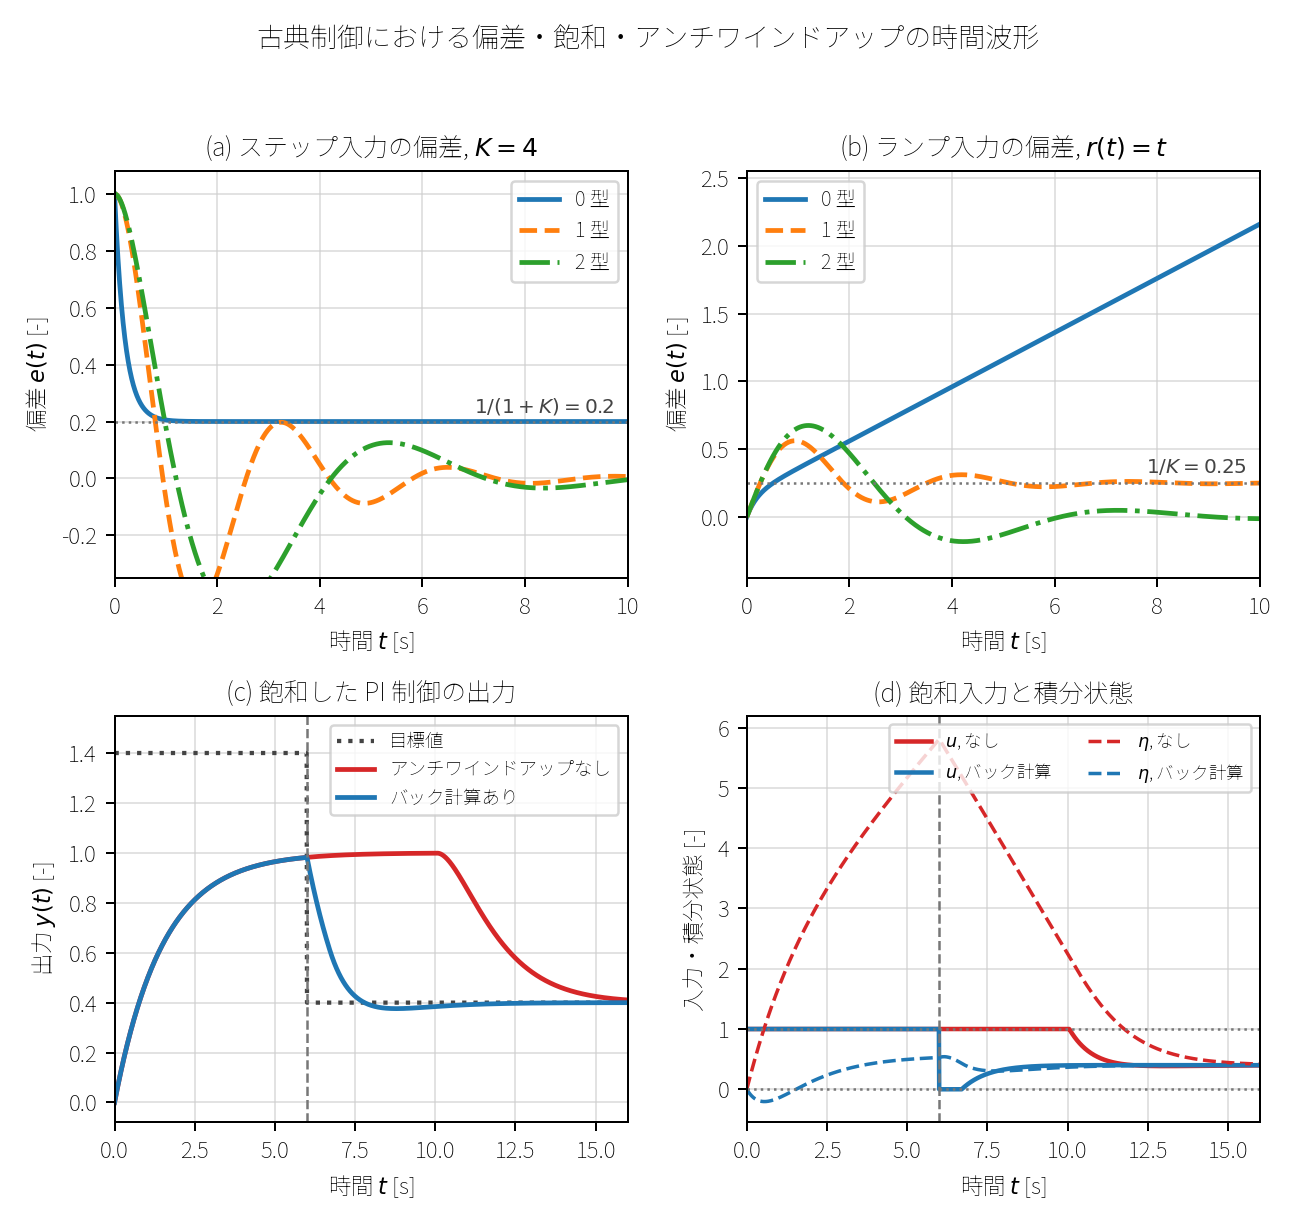
\includegraphics[width=0.96\linewidth,bb=0 0 1296 1224]{figures/classical_design_examples.png}
\caption{系の型による定常偏差と、飽和時の PI 制御におけるアンチワインドアップ効果。上段は $L_0(s)=4/(s+1)$、$L_1(s)=4/\{s(s+1)\}$、$L_2(s)=4(s+1)/\{s^2(s+4)\}$ の単位負帰還を同じ入力で比較し、型が上がると追従できる基準入力の次数が一つずつ上がることを示す。下段は $P(s)=1/(1.5s+1)$、$K_P=2.0$、$K_I=1.5$、$0\leq u\leq1$ の PI 制御で、バック計算が飽和中の積分状態を入力制約に合わせて戻すことを示す。}
\label{fig:classical-design-examples}
\end{figure}

\begin{practice}[定常偏差とアンチワインドアップの波形確認]
\wfig{classical-design-examples} の上段について、$K=4$ を用いて $0$ 型のステップ偏差 $1/(1+K)$ と $1$ 型のランプ偏差 $1/K$ を計算し、図中の水平破線と対応させよ。下段については、$t=6\,\mathrm{s}$ の直後に、アンチワインドアップなしの $\eta$ とバック計算ありの $\eta$ のどちらが $u_{\max}=1$ から大きく離れているかを読み取り、\weq{back-calculation-discrete} の補正項 $T_s(u_k-v_k)/T_t$ がその差を小さくする向きを説明せよ。
\end{practice}

\subsubsection{バンプレス切替}

手動運転から自動制御へ切り替えるとき、制御器内部の積分状態が現在の手動入力と整合していないと、切替瞬間に $u_c$ が段差を持つ。この段差を避けることをバンプレス切替という。切替時刻を $t_0$、手動で実際に入っている入力を $u_m(t_0)$ とする。二自由度 PID の内部状態は
\begin{equation}
  \eta(t_0^+)=u_m(t_0)-u_b
  -K_P\{\beta r(t_0)-y(t_0)\}
  -K_D\{\gamma d_r(t_0)-d_y(t_0)\}
  \label{eq:bumpless-initialization}
\end{equation}
に初期化する。これを \weq{two-degree-pid} に代入すると、切替直後の計算入力は $u_c(t_0^+)=u_m(t_0)$ となる。

手動運転中にも内部状態を追従させておく方法もある。手動入力に整合する積分状態を
\begin{equation}
  \eta_{tr}=u_m-u_b
  -K_P(\beta r-y)
  -K_D(\gamma d_r-d_y)
\end{equation}
と定義し、手動中は
\begin{equation}
  \dot{\eta}=\frac{1}{T_b}(\eta_{tr}-\eta)
\end{equation}
で更新する。$T_b$ は追従時定数で、単位は秒である。離散時間では後退オイラー近似により
\begin{equation}
  \eta_k=
  \frac{T_b}{T_b+T_s}\eta_{k-1}
  +\frac{T_s}{T_b+T_s}\eta_{tr,k}
\end{equation}
と更新できる。自動制御へ切り替える瞬間に $\eta_k=\eta_{tr,k}$ と代入してもよい。$T_b$ を十分小さくすれば、切替時に \weq{bumpless-initialization} とほぼ同じ状態になり、手動入力から自動入力へ連続に移れる。

\subsection{例：質量ばねダンパを古典制御で設計する}

質量 $m$、粘性 $c$、ばね $k$ の対象に力 $u$ を加える。
\begin{equation}
  m\ddot{q}+c\dot{q}+kq=u
\end{equation}
初期値 0 でラプラス変換すると
\begin{align}
  m s^2Q(s)+csQ(s)+kQ(s)&=U(s),\\
  (ms^2+cs+k)Q(s)&=U(s),\\
  G(s)=\frac{Q(s)}{U(s)}&=\frac{1}{ms^2+cs+k}.
\end{align}
標準形と比べるために分母を $m$ で割る。
\begin{equation}
  G(s)=\frac{1/m}{s^2+(c/m)s+k/m}.
\end{equation}
二次標準形 $s^2+2\zeta\omega_ns+\omega_n^2$ と係数を比べると
\begin{align}
  \omega_n^2&=k/m,\\
  2\zeta\omega_n&=c/m.
\end{align}
よって
\begin{align}
  \omega_n&=\sqrt{k/m},\\
  \zeta&=\frac{c}{2\sqrt{mk}}.
\end{align}
このように、物理パラメータ $m,c,k$ は応答仕様 $\omega_n,\zeta$ に直接つながる。重い質量は遅くし、大きな粘性は減衰を増やし、大きなばねは固有周波数を上げる。

比例制御 $u=K_p(r-q)$ を入れると
\begin{equation}
  m\ddot{q}+c\dot{q}+kq=K_p(r-q)
\end{equation}
である。整理して
\begin{equation}
  m\ddot{q}+c\dot{q}+(k+K_p)q=K_pr
\end{equation}
となる。閉ループの固有角周波数は
\begin{equation}
  \omega_{n,cl}=\sqrt{\frac{k+K_p}{m}}
\end{equation}
であり、減衰比は
\begin{equation}
  \zeta_{cl}=\frac{c}{2\sqrt{m(k+K_p)}}.
\end{equation}
したがって $K_p$ を大きくすると速くなるが、粘性 $c$ が変わらなければ減衰比は下がり、振動しやすくなる。これは「ゲインを上げると速いが振動する」という経験則の式による説明である。

比例制御の振動を抑えたいときは、変位の測定値から速度 $\dot{q}$ も使う。目標値をステップ状に変える例では、微分キックを避けるために微分を偏差ではなく測定値へかけ、
\begin{equation}
  u=K_p(r-q)-K_d\dot{q}
\end{equation}
とする。この PD 制御を代入すると
\begin{equation}
  m\ddot{q}+(c+K_d)\dot{q}+(k+K_p)q=K_pr
\end{equation}
である。閉ループの固有角周波数は比例制御と同じ
\begin{equation}
  \omega_{n,cl}=\sqrt{\frac{k+K_p}{m}}
\end{equation}
だが、減衰比は
\begin{equation}
  \zeta_{cl}=
  \frac{c+K_d}{2\sqrt{m(k+K_p)}}
\end{equation}
に変わる。したがって $K_d$ は、速さを大きく変えずに振動を抑える減衰として働く。ただし定常状態では $\dot{q}=0$ なので、PD 制御だけでは比例制御と同じ静的なばね負荷を残す。ステップ目標値 $r$ に対する定常値は
\begin{equation}
  q_\infty=\frac{K_p}{k+K_p}r
\end{equation}
であり、$k>0$ なら $q_\infty\neq r$ である。

定常偏差も消したい場合は、積分状態 $\eta$ を加えて
\begin{align}
  u&=K_p(r-q)+\eta-K_d\dot{q},\\
  \dot{\eta}&=K_I(r-q)
\end{align}
とする。一定目標値で閉ループが安定なら、定常状態では $\dot{\eta}=0$ だから $r-q=0$、すなわち $q=r$ である。このとき積分状態は、ばねをつり合わせるための力 $\eta=kr$ を供給する。偏差を消せる一方で、積分器は閉ループへ状態を一つ増やす。$r$ を一定として平衡点まわりの偏差を考えると、PID 候補の特性多項式は
\begin{equation}
  ms^3+(c+K_d)s^2+(k+K_p)s+K_I
\end{equation}
になる。三次の Routh-Hurwitz 判別法から、係数が正で
\begin{equation}
  (c+K_d)(k+K_p)>mK_I
\end{equation}
を満たすことが安定の基本条件になる。積分ゲイン $K_I$ を大きくすれば偏差の戻りは速くなるが、この条件と入力の大きさを同時に確認する必要がある。

\wfig{mass-spring-design-examples} は、同じ対象
\begin{equation}
  m=1\,\mathrm{kg},\qquad
  c=1\,\mathrm{N\,s/m},\qquad
  k=1\,\mathrm{N/m}
\end{equation}
に、$r=1\,\mathrm{m}$ のステップ目標値を与えた比較である。三つの候補は
\begin{equation}
  \begin{array}{c|ccc}
  \text{候補} & K_p & K_d & K_I\\ \hline
  \text{P} & 5 & 0 & 0\\
  \text{PD} & 5 & 3 & 0\\
  \text{PID} & 5 & 3 & 2
  \end{array}
\end{equation}
である。P 制御は初期の力が大きく、速く動くが、ばねを押し切る定常力が不足するため残留偏差を持つ。PD 制御は $K_d$ によって振動を抑えるが、低周波のゲインは P 制御と同じなので定常偏差は残る。PID 制御は積分状態がばね力を補うため目標値へ近づくが、操作力を長く使う。設計では、応答の速さだけでなく、終端偏差、最大力、RMS 操作力のような入力側の指標も同時に評価する。

\begin{figure}[tbp]
\centering
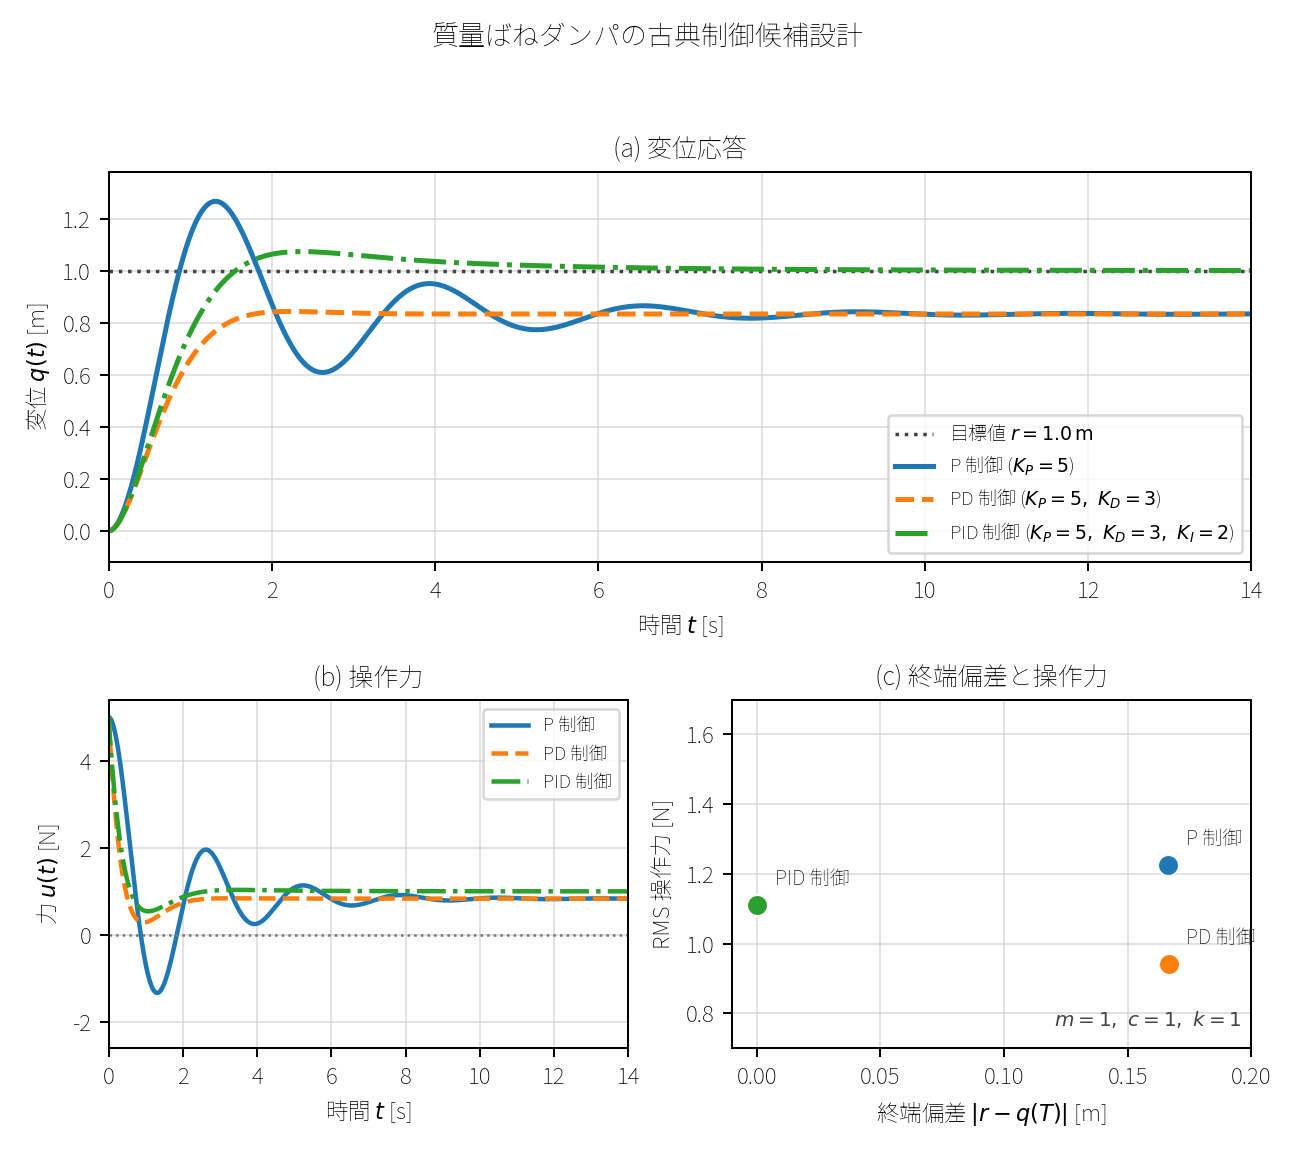
\includegraphics[width=0.96\linewidth,bb=0 0 1296 1152]{figures/mass_spring_design_examples.png}
\caption{質量ばねダンパ系に対する P、PD、PID 候補設計の比較。対象は $m=1\,\mathrm{kg}$、$c=1\,\mathrm{N\,s/m}$、$k=1\,\mathrm{N/m}$、目標値は $r=1\,\mathrm{m}$ である。PD 制御は速度フィードバックで振動を抑え、PID 制御は積分状態で定常偏差を減らすが、操作力の使い方も変わる。}
\label{fig:mass-spring-design-examples}
\end{figure}

\wfig{mass-spring-design-examples} の数値は、上の式だけでも読み取れる。P 制御と PD 制御では積分器がないので、一定目標値に対する定常力の釣合いは
\begin{equation}
  kq_\infty=K_p(r-q_\infty),\qquad
  q_\infty=\frac{K_p}{k+K_p}r=\frac{5}{6}\,\mathrm{m}
\end{equation}
である。したがって、どちらも目標値 $1\,\mathrm{m}$ に対して約 $0.167\,\mathrm{m}$ の残留偏差を持つ。PD 制御が改善しているのは定常値ではなく、二次閉ループの減衰である。固有角周波数は $\omega_n=\sqrt{(k+K_p)/m}=\sqrt{6}\,\mathrm{rad/s}$、減衰比は
\begin{equation}
  \zeta=\frac{c+K_d}{2\sqrt{m(k+K_p)}}
\end{equation}
だから、P 制御では $\zeta=1/(2\sqrt{6})\simeq0.204$、PD 制御では $\zeta=4/(2\sqrt{6})\simeq0.816$ になる。この増加が、上段の振動とオーバーシュートの小ささに対応している。

PID 候補では、積分ゲインを入れても Routh-Hurwitz 条件を満たす必要がある。ここでは
\begin{equation}
  (c+K_d)(k+K_p)=4\cdot6=24>mK_I=2
\end{equation}
であり、少なくとも三次線形モデルの安定条件は満たしている。図の下段右では、この安定な PID 候補が終端偏差をほぼ $0\,\mathrm{m}$ まで減らす一方、RMS 操作力は PD 制御の約 $0.94\,\mathrm{N}$ より大きい約 $1.11\,\mathrm{N}$ になっている。三候補はいずれも初期操作力が $u(0)=K_pr=5\,\mathrm{N}$ で、ピーク力だけでは差が出ない。このため、同じピーク力の範囲でも、PD 制御は平均的な入力を抑えて振動を減らし、PID 制御は残留偏差を消す代わりに操作力を長く使う、という入力側のトレードオフが残る。

\subsection{参照値整形とレート制限}

入力飽和とアンチワインドアップを入れると、制御器の内部状態はアクチュエータの限界と矛盾しにくくなる。しかし、それだけでは目標値そのものが物理的に実行可能になるわけではない。DC モータの位置サーボで、軸角度を今すぐ $1\,\mathrm{rad}$ だけ動かすステップ目標値を与えた場合を考える。積分器が暴走しなくても、ステップ目標値は瞬間的な位置変化を要求するので、有限の電圧、電流、トルクしか出せないモータには追従できない。

簡単な検証対象として、角度を $\theta(t)\,[\mathrm{rad}]$、角速度を $\omega(t)\,[\mathrm{rad/s}]$、モータへ印加される電圧を $u(t)\,[\mathrm{V}]$ とし、動作点近傍で
\begin{align}
  \dot{\theta}&=\omega,\\
  J\dot{\omega}&=K_tu-b\omega,
  \qquad |u|\leq u_{max}
  \label{eq:reference-shaping-motor-model}
\end{align}
と近似する。ここで $J\,[\mathrm{kg\,m^2}]$ は慣性、$b\,[\mathrm{N\,m\,s/rad}]$ は粘性係数、$K_t\,[\mathrm{N\,m/V}]$ は電圧からトルクへの比例係数、$u_{max}\,[\mathrm{V}]$ は電圧上限である。位置制御器は、目標値経路から作った実際の参照値を $r_a(t)\,[\mathrm{rad}]$ として
\begin{align}
  u_c&=K_p(r_a-\theta)-K_d\omega,\\
  u&=\operatorname{sat}_{[-u_{max},u_{max}]}(u_c)
  \label{eq:reference-shaping-position-servo}
\end{align}
とする。$K_p$ の単位は $\mathrm{V/rad}$、$K_d$ の単位は $\mathrm{V/(rad/s)}$ である。微分は測定速度側に置き、目標値ステップによる微分キックは避けている。積分項を加える場合でも、アンチワインドアップは $u_c$ と $u$ の差を内部状態へ戻す処理であり、式 \eqref{eq:reference-shaping-position-servo} が飽和を受ける事実は残る。

生のステップ目標値は
\begin{equation}
  r_{step}(t)=r_0+\Delta r\,H(t-t_0)
\end{equation}
で表せる。$H$ は単位ステップであり、形式的な速度は
\begin{equation}
  \dot{r}_{step}(t)=\Delta r\,\delta(t-t_0)
\end{equation}
になる。これは、目標角度の速度が瞬間だけ無限大になることを意味する。モータ側では $|\dot{\omega}(0)|\leq K_tu_{max}/J$ なので、この要求は最初から実現できない。さらに、初期状態が $\theta=r_0,\omega=0$ なら、式 \eqref{eq:reference-shaping-position-servo} の直後の指令は
\begin{equation}
  u_c(t_0^+)=K_p\Delta r
\end{equation}
である。$|K_p\Delta r|>u_{max}$ なら、最初の計算から飽和が確定する。

この問題を、制御器ゲインだけで直すと、応答全体を遅くすることになりやすい。別の考え方は、外から来た目標値 $r_{cmd}$ をそのまま制御器へ入れず、モータが追従しやすい参照値 $r_a$ へ変換してから入れることである。この変換を参照値整形という。最も単純な整形は、時定数 $\tau_r\,[\mathrm{s}]$ の一次遅れ
\begin{equation}
  \tau_r\dot{r}_f=r_{cmd}-r_f,
  \qquad r_a=r_f
  \label{eq:first-order-reference-shaping}
\end{equation}
である。$r_{cmd}$ と $r_f$ の単位は同じ $\mathrm{rad}$ で、$\dot{r}_f$ の単位は $\mathrm{rad/s}$ である。$t=t_0$ で $r_0$ から $r_0+\Delta r$ へ変わるステップに対し、$t\geq t_0$ では
\begin{align}
  r_f(t)&=r_0+\Delta r\{1-\exp(-(t-t_0)/\tau_r)\},\\
  \dot{r}_f(t)&=\frac{\Delta r}{\tau_r}
  \exp(-(t-t_0)/\tau_r)
  \label{eq:first-order-reference-step}
\end{align}
となる。したがって初期の最大参照速度は $|\Delta r|/\tau_r$ である。$\tau_r$ を大きくすると速度要求は下がるが、目標値へ近づく時間は長くなる。

もう一つのよく使う実装は、サンプリング周期 $T_s\,[\mathrm{s}]$ ごとに変化量を制限するレートリミッタである。最大速度を $v_{max}\,[\mathrm{rad/s}]$ として
\begin{equation}
  r_{\ell,k+1}
  =
  r_{\ell,k}
  +
  \operatorname{clip}
  \left(
    r_{cmd,k}-r_{\ell,k},
    -v_{max}T_s,
    v_{max}T_s
  \right),
  \qquad r_a=r_\ell
  \label{eq:rate-limited-reference}
\end{equation}
と更新する。ここで $\operatorname{clip}(x,a,b)$ は $x$ を区間 $[a,b]$ に収める演算である。ステップ目標値に対しては、符号を除けば傾き $v_{max}$ のランプになり、移動時間は少なくとも $|\Delta r|/v_{max}$ になる。一次整形は指数関数的に滑らかに目標へ近づき、レート制限は最大速度を明示的に守る、という違いがある。

参照値がアクチュエータ制約と矛盾しているかどうかは、飽和後の入力だけを見ると分かりにくい。飽和後の $u$ は必ず範囲内に収まるからである。そこで、飽和前の指令余裕
\begin{equation}
  \mu_c(t)=1-\frac{|u_c(t)|}{u_{max}}
  \label{eq:command-margin-reference-shaping}
\end{equation}
を使う。$\mu_c(t)>0$ なら指令は電圧範囲内にあり、$\mu_c(t)=0$ はちょうど上限、$\mu_c(t)<0$ は制御器が実現できない電圧を要求している状態である。

\wfig{reference-shaping-rate-limit-examples} は、式 \eqref{eq:reference-shaping-motor-model} と式 \eqref{eq:reference-shaping-position-servo} を
\begin{equation}
  J=1.0,\quad b=0.55,\quad K_t=1.0,\quad
  u_{max}=2.2,\quad K_p=10.0,\quad K_d=3.2
\end{equation}
で計算した例である。目標値は $t_0=0.30\,\mathrm{s}$ で $\Delta r=1.0\,\mathrm{rad}$ だけ変わる。生ステップでは $u_c(t_0^+)=10.0\,\mathrm{V}$ となり、上限 $2.2\,\mathrm{V}$ の約 $4.5$ 倍を要求するため、指令余裕は大きく負になる。一次整形で $\tau_r=0.60\,\mathrm{s}$ とすると、最大参照速度は $1.67\,\mathrm{rad/s}$ になり、最小余裕はほぼ $0$ の近くまで改善する。レート制限で $v_{max}=0.90\,\mathrm{rad/s}$ とすると、余裕をさらに残したまま応答する。

\begin{figure}[tbp]
\centering
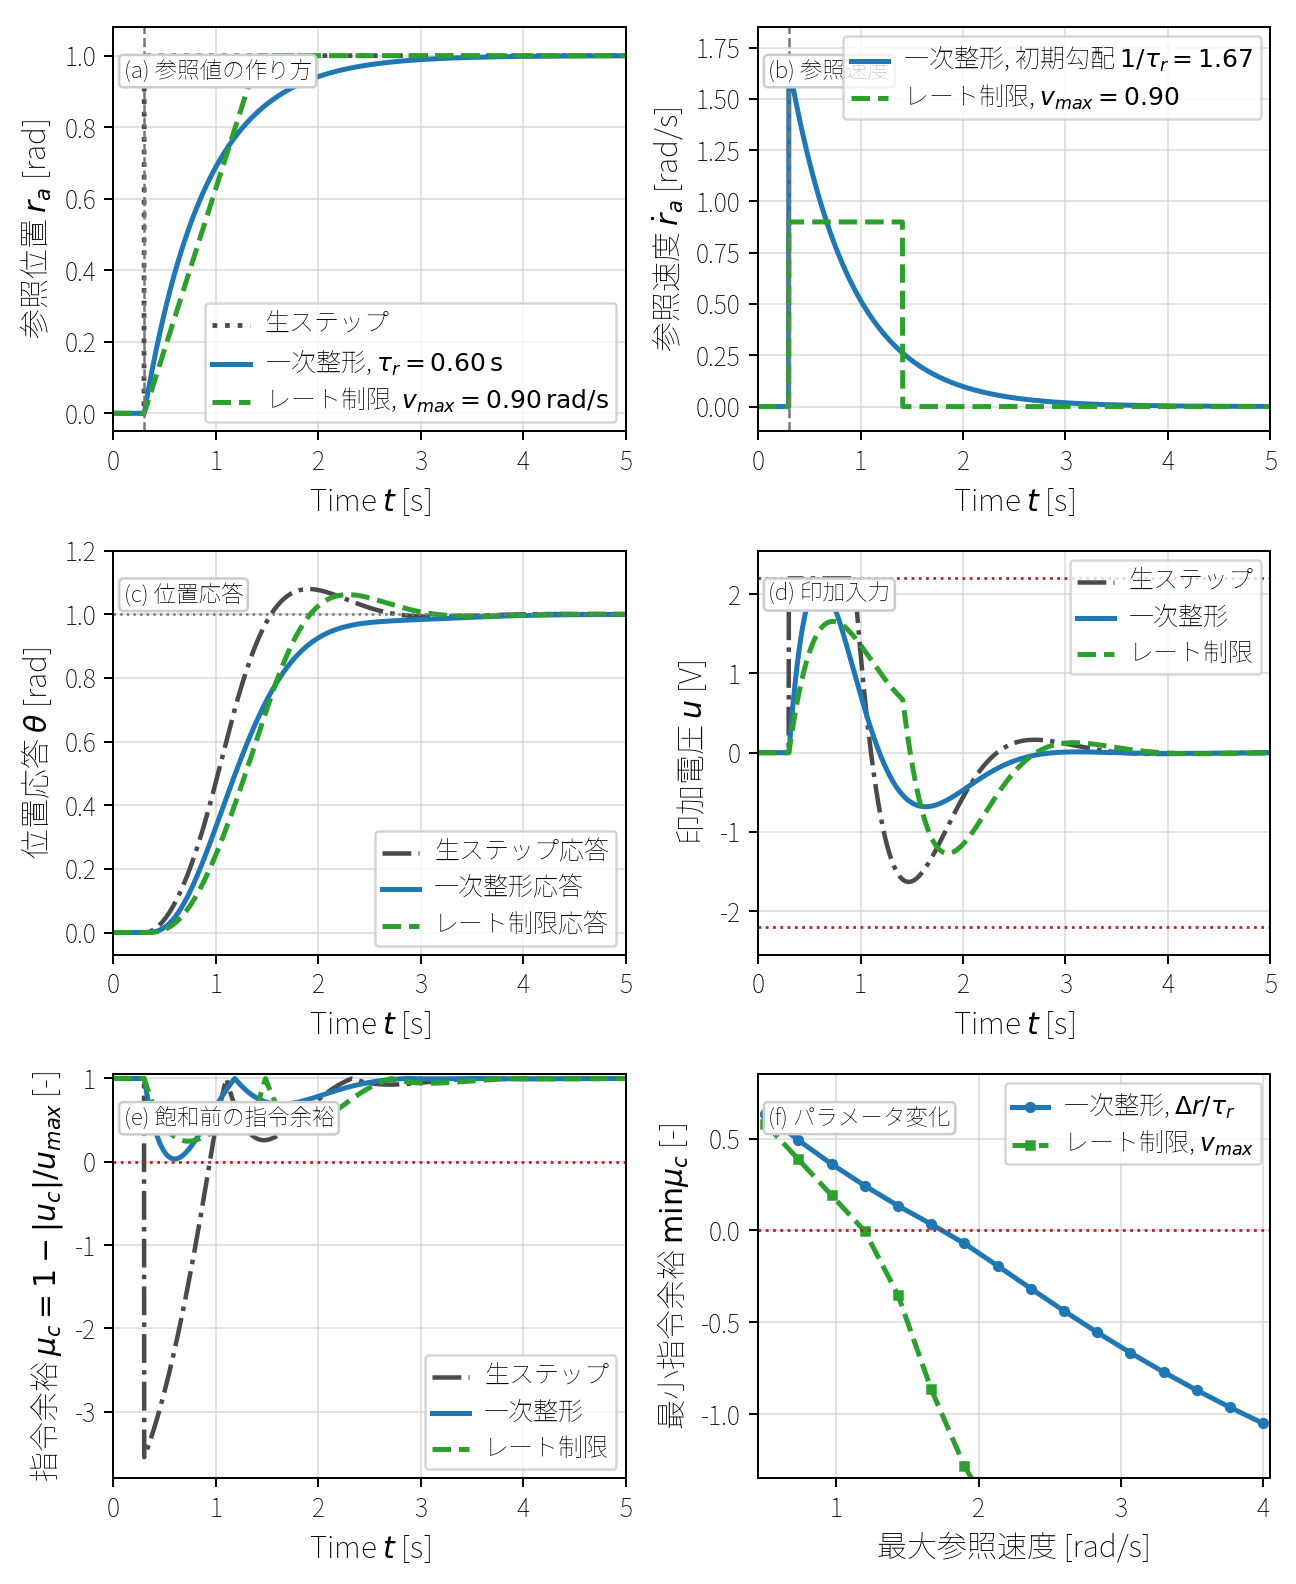
\includegraphics[width=0.96\linewidth,bb=0 0 1296 1584]{figures/reference_shaping_rate_limit_examples.png}
\caption{DC モータ位置サーボに対する参照値整形とレート制限の比較。生ステップは位置目標を瞬時に変えるため、飽和前の電圧指令が上限を大きく越える。一次整形は時定数 $\tau_r$ で参照速度を有限にし、レート制限は $v_{max}$ で参照速度そのものを制限する。下段右は最大参照速度を変えたときの最小指令余裕であり、速い参照ほど余裕が減ることを表している。}
\label{fig:reference-shaping-rate-limit-examples}
\end{figure}

パラメータの役割は、応答の見た目ではなく、制約余裕と移動時間の両方で解釈する。一次整形では、$\tau_r$ を小さくすると $|\Delta r|/\tau_r$ が大きくなり、参照値は速く立ち上がるが、図の下段右のように $\min\mu_c$ は低下する。$\tau_r=0.25\,\mathrm{s}$ のように初期勾配が $4.0\,\mathrm{rad/s}$ になる設定では、この例の電圧上限を再び越える。一方、$\tau_r$ を大きくすると余裕は増えるが、目標値自体が遅くなるため、整定時間は参照値整形器によって決まる。レート制限でも同じで、$v_{max}$ を大きくすれば移動は短くなるが、指令余裕は小さくなる。$v_{max}$ を小さくすると制約には優しくなるが、移動時間 $|\Delta r|/v_{max}$ が直接長くなる。

したがって、参照値整形とレート制限は「応答を丸めるための見た目の処理」ではなく、制御問題の入力側を実現可能な問題へ変換する処理である。アンチワインドアップは、飽和が起きた後に積分器が誤った内部状態を持ち続けることを防ぐ。参照値整形は、その前段で、飽和を起こしにくい目標値を作る。実機では、位置の最大速度だけでなく、電流上限、電圧上限、温度上昇、機械的な衝撃も同時に制約になるため、一次整形や単純なレート制限で足りない場合は、加速度制限や S 字軌道へ進むことになる。

\subsection{DC モータサーボのカスケード制御と電流・電圧限界}

目標値の整形とレート制限を入れると、位置指令や速度指令は急な段差を持たなくなる。それでも、アクチュエータが実際に出せる電流、電圧、トルクには上限がある。ここでは、軸の位置を合わせる DC モータサーボを使い、電圧が電流を作り、電流がトルクを作り、トルクが速度と位置を変えるという物理の順序に沿って、電流ループ、速度ループ、位置ループを分ける。

直前までの PID とアンチワインドアップでは、計算入力 $u_c$ と印加入力 $u$ の差を一つの飽和器として扱った。DC モータでは、その飽和器の内側に少なくとも二つの制約がある。一つは巻線・インバータ・電源で決まる電流上限、もう一つは逆起電力と抵抗降下を含む電圧上限である。これらを分けて見ないと、外側の位置制御器が「もっと大きなトルクを出せば速く追従できる」と計算していても、内側の電流ループが実現できない理由を説明できない。

\subsubsection{DC モータで分かれる三つの信号}

剛体軸に接続された DC モータを、次の単純化モデルで扱う。
\begin{align}
  L\dot{i}+Ri+K_e\omega&=v,\\
  J\dot{\omega}+b\omega&=K_t i-\tau_L,\\
  \dot{\theta}&=\omega.
  \label{eq:cascade-dc-motor}
\end{align}
$v$ は端子電圧 $[\mathrm{V}]$、$i$ は電機子電流 $[\mathrm{A}]$、$\tau_m=K_t i$ はモータトルク $[\mathrm{N\,m}]$、$\omega$ は角速度 $[\mathrm{rad/s}]$、$\theta$ は角度 $[\mathrm{rad}]$ である。$R[\Omega]$、$L[\mathrm{H}]$、$K_e[\mathrm{V\,s/rad}]$、$K_t[\mathrm{N\,m/A}]$、$J[\mathrm{kg\,m^2}]$、$b[\mathrm{N\,m\,s/rad}]$ は正の定数とする。ここではクーロン摩擦、デッドゾーン、バックラッシュは入れない。これらは電流・電圧制約の後に残る別の実装限界として次に扱う。

電気式の左辺を見ると、電圧 $v$ は三つの成分に使われる。$L\dot{i}$ は電流を速く変えるための電圧、$Ri$ は巻線抵抗で消費される電圧、$K_e\omega$ は回転速度に比例する逆起電力である。したがって、同じ電流指令でも、低速でゆっくり変えるときと、高速で急に増やすときでは必要電圧が違う。機械式では、電流 $i$ がトルク $K_t i$ へ変換され、そのトルクから粘性抵抗 $b\omega$ と負荷トルク $\tau_L$ を差し引いたものが角加速度 $J\dot{\omega}$ を決める。

この信号の順序から、自然なカスケード構造は次の三段になる。
\begin{align}
  \text{位置ループ:}\quad
  \omega_r&=C_\theta(s)(\theta_r-\theta),\\
  \text{速度ループ:}\quad
  i_r^c&=C_\omega(s)(\omega_r-\omega),\\
  \text{電流ループ:}\quad
  v_c&=C_i(s)(i_r-i).
  \label{eq:cascade-loop-signals}
\end{align}
$\theta_r$ の単位は $[\mathrm{rad}]$、$\omega_r$ の単位は $[\mathrm{rad/s}]$、$i_r^c$ と $i_r$ の単位は $[\mathrm{A}]$、$v_c$ の単位は $[\mathrm{V}]$ である。速度ループの出力は、物理的には「出したいトルクを電流で表した量」である。電流ループの出力は、その電流を実現するための電圧指令である。

\begin{figure}[tbp]
\centering
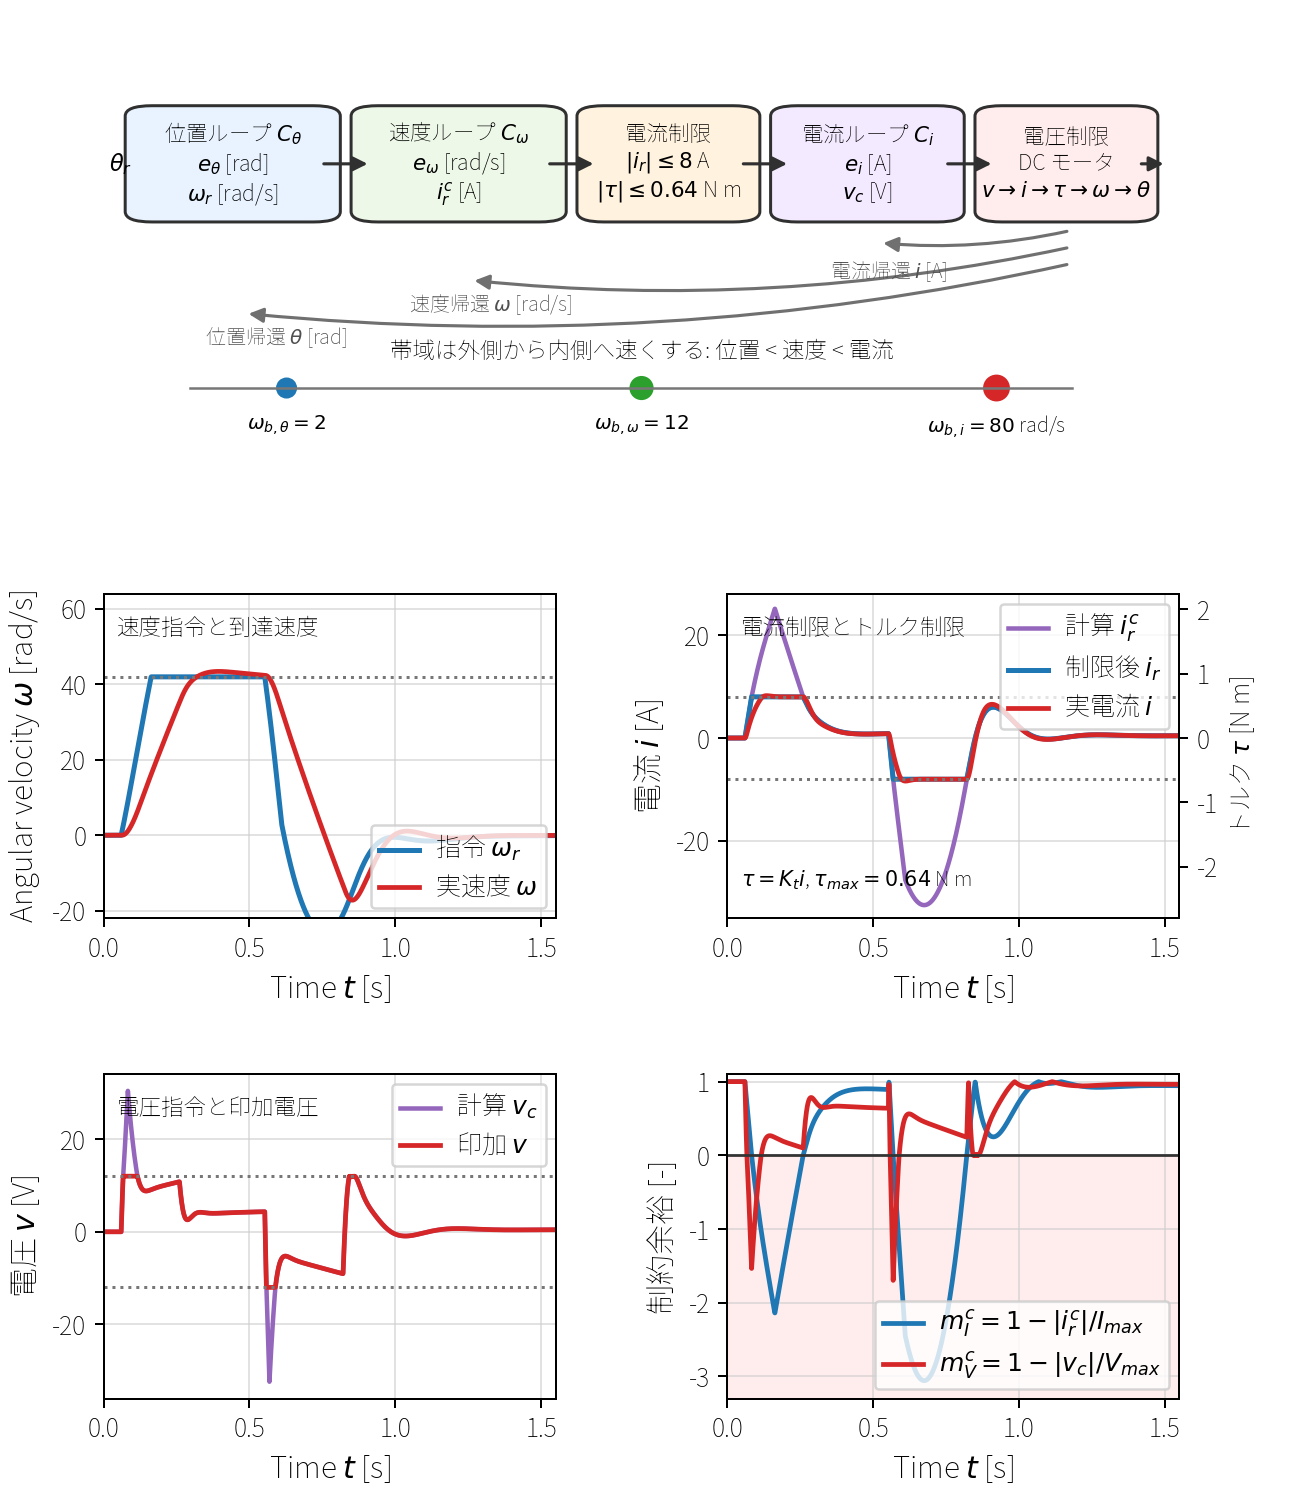
\includegraphics[width=0.98\linewidth,bb=0 0 1296 1512]{figures/cascade_actuator_limits_examples.png}
\caption{DC モータ位置サーボのカスケード構成と電流・電圧限界。上段は位置、速度、電流の三つのループを外側から内側へ配置し、帯域幅を $\omega_{b,\theta}=2\,\mathrm{rad/s}$、$\omega_{b,\omega}=12\,\mathrm{rad/s}$、$\omega_{b,i}=80\,\mathrm{rad/s}$ の順に速くした例である。下段は $R=1.0\,\Omega$、$L=0.050\,\mathrm{H}$、$K_t=K_e=0.08$、$J=0.003\,\mathrm{kg\,m^2}$、$b=0.002\,\mathrm{N\,m\,s/rad}$、$I_{\max}=8\,\mathrm{A}$、$V_{\max}=12\,\mathrm{V}$ としたシミュレーションで、速度指令、電流指令、印加電圧、制約余裕を同じ時間軸で示す。電流指令 $i_r^c$ と電圧指令 $v_c$ の余裕が 0 を下回る時間帯では、外側ループが要求したトルク変化を内側ループが実現できない。}
\label{fig:cascade-actuator-limits-examples}
\end{figure}

\wfig{cascade-actuator-limits-examples} の上段は、三つの信号をどのループが作るかを示している。位置制御器は速度指令を作るだけであり、直接電圧を決めない。速度制御器は電流指令を作るだけであり、直接位置を動かすわけではない。電流制御器だけが電圧を出し、その電圧がモータ巻線と逆起電力を通して実電流を変える。この分担を明確にすると、飽和がどの信号で起きたのかを分けて読める。

\subsubsection{帯域分離と等価対象}

内側電流ループが閉ループ伝達関数
\begin{equation}
  T_i(s)=\frac{I(s)}{I_r(s)}
\end{equation}
で表されるとする。外側の速度ループが使う周波数範囲で
\begin{equation}
  T_i(j\omega)\simeq 1,
  \qquad
  \angle T_i(j\omega)\simeq 0
  \quad (0\leq\omega\leq\omega_{b,\omega})
  \label{eq:current-loop-fast-condition}
\end{equation}
なら、速度ループから見ると $i\simeq i_r$ と近似できる。このとき \weq{cascade-dc-motor} の機械式は
\begin{align}
  J\dot{\omega}+b\omega
  &\simeq K_t i_r-\tau_L
\end{align}
であり、負荷トルクをいったん 0 とおくと、電流指令から速度までの等価対象は
\begin{equation}
  \frac{\Omega(s)}{I_r(s)}
  \simeq
  \frac{K_t}{Js+b}
  \label{eq:current-to-speed-equivalent}
\end{equation}
になる。さらに位置は $\dot{\theta}=\omega$ なので、
\begin{equation}
  \frac{\theta(s)}{I_r(s)}
  \simeq
  \frac{K_t}{s(Js+b)}
  \label{eq:current-to-position-equivalent}
\end{equation}
である。位置ループはこの二重の遅れを相手にするため、速度ループより遅く置く。

帯域幅を、位置ループ $\omega_{b,\theta}$、速度ループ $\omega_{b,\omega}$、電流ループ $\omega_{b,i}$ と書く。設計の目安は
\begin{equation}
  \omega_{b,i}\geq 5\omega_{b,\omega},
  \qquad
  \omega_{b,\omega}\geq 5\omega_{b,\theta}
  \label{eq:cascade-bandwidth-order}
\end{equation}
である。これは厳密な定理ではなく、外側ループが内側ループをほぼ比例要素として扱える範囲を確保するための実務的な条件である。\wfig{cascade-actuator-limits-examples} の上段では、$2$、$12$、$80\,\mathrm{rad/s}$ としてこの順序を示した。内側を速くしすぎると、電流測定ノイズ、PWM 遅れ、電圧飽和の影響が増えるため、帯域を上げるほどよいわけではない。

\subsubsection{電流・トルク・電圧・速度の限界}

速度ループが計算した電流指令を $i_r^c$ とする。インバータ、巻線温度、電源容量から連続または短時間の電流上限 $I_{\max}$ が決まると、電流ループに渡す指令は
\begin{equation}
  i_r=\operatorname{sat}_{[-I_{\max},I_{\max}]}(i_r^c)
  \label{eq:current-command-limit}
\end{equation}
である。トルクは $\tau_m=K_t i$ なので、電流制限は同時に
\begin{equation}
  |\tau_m|\leq K_t I_{\max}
  \label{eq:torque-current-limit}
\end{equation}
というトルク制限でもある。図の例では $I_{\max}=8\,\mathrm{A}$、$K_t=0.08\,\mathrm{N\,m/A}$ だから、到達できるトルクは $0.64\,\mathrm{N\,m}$ までである。速度ループが $i_r^c=15\,\mathrm{A}$ を計算しても、モータへは $8\,\mathrm{A}$ 相当のトルクしか要求できない。

一方、電流が制限内でも、電圧上限が先に効くことがある。\weq{cascade-dc-motor} の電気式を電圧について解くと
\begin{equation}
  v=L\dot{i}+Ri+K_e\omega
  \label{eq:voltage-required-current}
\end{equation}
である。電源電圧を $V_{\max}$ とすると、印加電圧は
\begin{equation}
  v=\operatorname{sat}_{[-V_{\max},V_{\max}]}(v_c)
  \label{eq:voltage-command-limit}
\end{equation}
になる。電流を速く増やしたいときは $L\dot{i}$ が大きくなり、高速回転中は $K_e\omega$ が大きくなる。したがって、低速では実現できた同じ電流指令が、高速では逆起電力のために実現できない場合がある。準定常で $\dot{i}\simeq0$ と見なせるなら、
\begin{equation}
  |Ri+K_e\omega|\leq V_{\max}
  \label{eq:steady-voltage-limit}
\end{equation}
が必要である。正転で正電流を流すときは、概略的に
\begin{equation}
  \omega\leq\frac{V_{\max}-Ri}{K_e}
  \label{eq:voltage-speed-current-limit}
\end{equation}
となり、速度が上がるほど同時に出せる電流、つまりトルクが小さくなる。

図の下段では、計算電流 $i_r^c$ は最初の加速区間で $I_{\max}$ を超えている。制限後の $i_r$ は $8\,\mathrm{A}$ で頭打ちになり、実電流 $i$ はさらに電圧上限と巻線時定数のために遅れて立ち上がる。電圧指令 $v_c$ は $V_{\max}=12\,\mathrm{V}$ を大きく超える時間帯があり、印加電圧 $v$ は上限に張り付く。制約余裕
\begin{equation}
  m_I^c=1-\frac{|i_r^c|}{I_{\max}},
  \qquad
  m_V^c=1-\frac{|v_c|}{V_{\max}}
  \label{eq:constraint-margin}
\end{equation}
は、計算指令が制約内なら正、制約ちょうどなら 0、実現不能なら負になる。余裕が負になっている時間帯では、外側ループの計算結果をそのまま物理入力として扱ってはいけない。

\subsubsection{電流ループ飽和時に崩れる前提}

カスケード制御の外側ループは、内側の電流ループが \weq{current-loop-fast-condition} を満たし、$i\simeq i_r$ になることを前提にしている。電圧飽和または電流制限に入ると、この前提が崩れる。実際の電流変化は
\begin{equation}
  \dot{i}
  =
  \frac{
  \operatorname{sat}_{[-V_{\max},V_{\max}]}(v_c)-Ri-K_e\omega
  }{L}
  \label{eq:saturated-current-dynamics}
\end{equation}
で決まり、制御器が計算した $v_c$ ではなく、飽和後の電圧でしか動かない。つまり、内側閉ループはもはや速い比例要素ではなく、電圧上限に張り付いた非線形な電流立上りになる。

このとき速度ループには、必要なトルクが出ていないことが速度偏差の残りとして現れる。速度ループや位置ループに積分器があると、その偏差を消そうとしてさらに大きな電流指令を蓄積し、外側のワインドアップを起こす。したがって、電流制限を入れるだけでは不十分であり、制限後の $i_r$ と実電流 $i$ の情報を外側のアンチワインドアップへ戻す必要がある。速度ループの積分状態を、$i_r^c-i_r$ または実トルク不足 $K_t(i_r-i)$ に応じて戻す構成にすると、外側ループは「トルクがまだ出ていない」ことを内部状態にも反映できる。

もう一つの失敗は帯域順序の見かけ上の崩れである。線形設計では $\omega_{b,i}$ が十分大きくても、飽和中の電流変化率は \weq{saturated-current-dynamics} の上限で決まる。電流が遅れている時間帯では、速度ループが期待した位相とゲインが得られない。位置ループは速度ループの遅れを、速度ループは電流ループの遅れを、それぞれ未知の対象遅れとして受け取るため、振動や行き過ぎが増える。

ここまでで、目標値を滑らかにしても、電流、トルク、電圧、速度の制約が実現可能な応答を決めることが分かった。次に残る限界は、制約内の小さな電圧やトルクを出しているにもかかわらず、静止摩擦、デッドゾーン、バックラッシュのために軸が思った通り動かない場合である。したがって、次の段階では、電流・電圧の上限ではなく、入力と運動の間にある不感帯と履歴を分けて扱う。

\subsection{摩擦・不感帯・バックラッシの測定と補償}

電流制限と電圧制限を考慮すると、指令がアクチュエータの許容範囲を越えないようにできる。
しかし、許容範囲内の小さな指令が、そのまま小さな運動になるとは限らない。
DC モータをギヤで減速した位置サーボでは、低速で止まりかけたときに静止摩擦が効き、ドライバや機構の不感帯によって小さな電圧指令が出力へ届かず、回転方向を反転した直後にはギヤのバックラッシを詰めるまで負荷側が遅れる。
したがって、前段までの飽和対策で
\[
  |v|\leq V_{\max},\qquad |\tau_c|\leq \tau_{\max}
\]
を守っていても、測定された負荷角 $\theta_l$ は目標角 $\theta_{l,r}$ に追従しない場合がある。
ここで $v$ はモータドライバへの電圧指令 $[\mathrm{V}]$、$\tau_c$ は電流ループまたはトルク制御器が作るモータ軸トルク指令 $[\mathrm{N\,m}]$、$\omega$ はモータ角速度 $[\mathrm{rad/s}]$、$\theta_m$ はモータ軸角 $[\mathrm{rad}]$、$\theta_l$ は負荷側角 $[\mathrm{rad}]$ である。

以下では、内側の電流ループは外側の位置ループより十分速く、低速域では温度と荷重が短時間で大きく変わらないと仮定する。
また、軸の弾性変形はバックラッシ幅に比べて小さく、摩擦・不感帯・バックラッシは一軸の測定曲線として扱えるとする。
この仮定は補償式を作るための近似であり、摩擦やすきまを物理的に消す仮定ではない。

\subsubsection{低速掃引による非線形特性の測定}

まず、負荷を外さずに低速で正負方向へ掃引し、静止摩擦、動摩擦、不感帯、バックラッシを別々に測る。
\wfig{friction-deadzone-backlash-examples} は、次の数値を持つ小形 DC モータサーボの低速測定例である。
\[
  \tau_s=0.16\,\mathrm{N\,m},\qquad
  \tau_k=0.105\,\mathrm{N\,m},\qquad
  b=0.018\,\mathrm{N\,m\,s/rad},
\]
\[
  v_d=0.72\,\mathrm{V},\qquad
  K_v=8.0\,\mathrm{rad/(s\,V)},\qquad
  \Delta_\theta=0.18\,\mathrm{rad}.
\]
$\tau_s$ は止まっている軸を動かし始めるための静止摩擦トルク、$\tau_k$ は動き始めた後の Coulomb 摩擦トルク、$b$ は粘性摩擦係数、$v_d$ は不感帯の片側幅、$K_v$ は不感帯を越えた後の低速ゲイン、$\Delta_\theta$ は負荷側に現れるバックラッシ幅である。

低速で一定角速度 $\omega$ を保つために必要なトルクを測ると、動いている範囲では
\[
  \tau_{\mathrm{meas}}(\omega)
  \simeq b\omega+\tau_k\operatorname{sgn}(\omega),
  \qquad \omega\neq 0
\]
と近似できる。
一方、静止中は一つの値ではなく区間として扱う。
外乱トルクを含めた駆動側の差し引きトルクが
\[
  -\tau_s \leq \tau_{\mathrm{drive}}-\tau_{\mathrm{load}}\leq \tau_s
\]
に入ると、角速度は $\omega=0$ のままになり得る。
このため、比例制御器が小さな偏差から小さなトルクを作っても、そのトルクが静止摩擦帯の内側なら運動は始まらない。

ドライバの不感帯は、電圧指令 $v$ と定常角速度 $\omega_{\mathrm{ss}}$ の測定から
\[
  \omega_{\mathrm{ss}}(v)
  \simeq
  K_v\operatorname{sgn}(v)\max\{|v|-v_d,0\}
\]
と近似する。
この式は、$|v|\leq v_d$ では電圧指令を変えても定常角速度がほぼ 0 であり、$|v|>v_d$ になってから傾き $K_v$ の直線に近づくことを表す。
電圧制限 $|v|\leq V_{\max}$ を守っていても、$v_d$ より小さい指令しか出ていないなら、実機には入力が入っていないのと同じ状態が生じる。

バックラッシは、モータ軸をゆっくり往復させて、モータ軸角 $\theta_m$ と負荷側角 $\theta_l$ の閉じない曲線として測る。
単純なすきまモデルでは、接触面が正転側に当たっているとき
\[
  \theta_l\simeq \theta_m-\frac{\Delta_\theta}{2},
\]
逆転側に当たっているとき
\[
  \theta_l\simeq \theta_m+\frac{\Delta_\theta}{2}
\]
である。
その間の区間では、モータ軸だけが動いても負荷側がまだ動かない。
方向反転の直後に負荷角の応答が遅れるのは、このすきまを詰める運動が先に必要になるためである。

\subsubsection{逆特性を用いた補償入力}

補償では、測定した非線形特性の逆向きの入力を、線形フィードバックの外側または前置補償として加える。
符号関数をそのまま使うとゼロ付近で入力が急に切り替わり、量子化やノイズで微小振動を起こしやすい。
そこで
\[
  \sigma_\epsilon(x)=\tanh\left(\frac{x}{\epsilon}\right)
\]
を滑らかな符号近似として使う。
速度目標 $\omega_r$ に対する摩擦補償トルクは
\[
  \tau_{\mathrm{fric}}(\omega_r)
  =b\omega_r+\tau_k\sigma_{\epsilon_\omega}(\omega_r)
\]
と置ける。
線形制御器が作る等価電圧を $v_\ell$ とし、モータトルク定数を $K_t\,[\mathrm{N\,m/V}]$ とまとめて表すと、不感帯と摩擦を含む電圧補償は
\[
  v_c
  =
  \operatorname{sat}_{[-V_{\max},\,V_{\max}]}
  \left(
    v_\ell
    +v_d\sigma_{\epsilon_v}(v_\ell)
    +\frac{\tau_{\mathrm{fric}}(\omega_r)}{K_t}
  \right)
\]
である。
飽和関数 $\operatorname{sat}_{[-V_{\max},\,V_{\max}]}(\cdot)$ は、補償を加えた後でも電圧制限を越えないために残しておく。
補償項が大きすぎて飽和に当たる場合、静止摩擦や不感帯の一部は補えず、前節までの制限が再び支配的になる。

バックラッシは、目標負荷角 $\theta_{l,r}$ に対して、接触させたい側へモータ軸目標を先にずらす。
負荷側の目標速度を $\dot{\theta}_{l,r}$ とすると、
\[
  \theta_{m,r}^{\mathrm{comp}}
  =
  \theta_{l,r}
  +\frac{\Delta_\theta}{2}
  \sigma_{\epsilon_\theta}(\dot{\theta}_{l,r})
\]
である。
正転中はモータ軸目標を負荷側目標より $\Delta_\theta/2$ だけ進め、逆転中は同じ量だけ戻す。
この補償は、どちらの歯面へ接触させたいかをあらかじめ決める操作であり、負荷側がすきまの中で自由に動く瞬間を完全にはなくせない。

\begin{figure}[tbp]
\centering
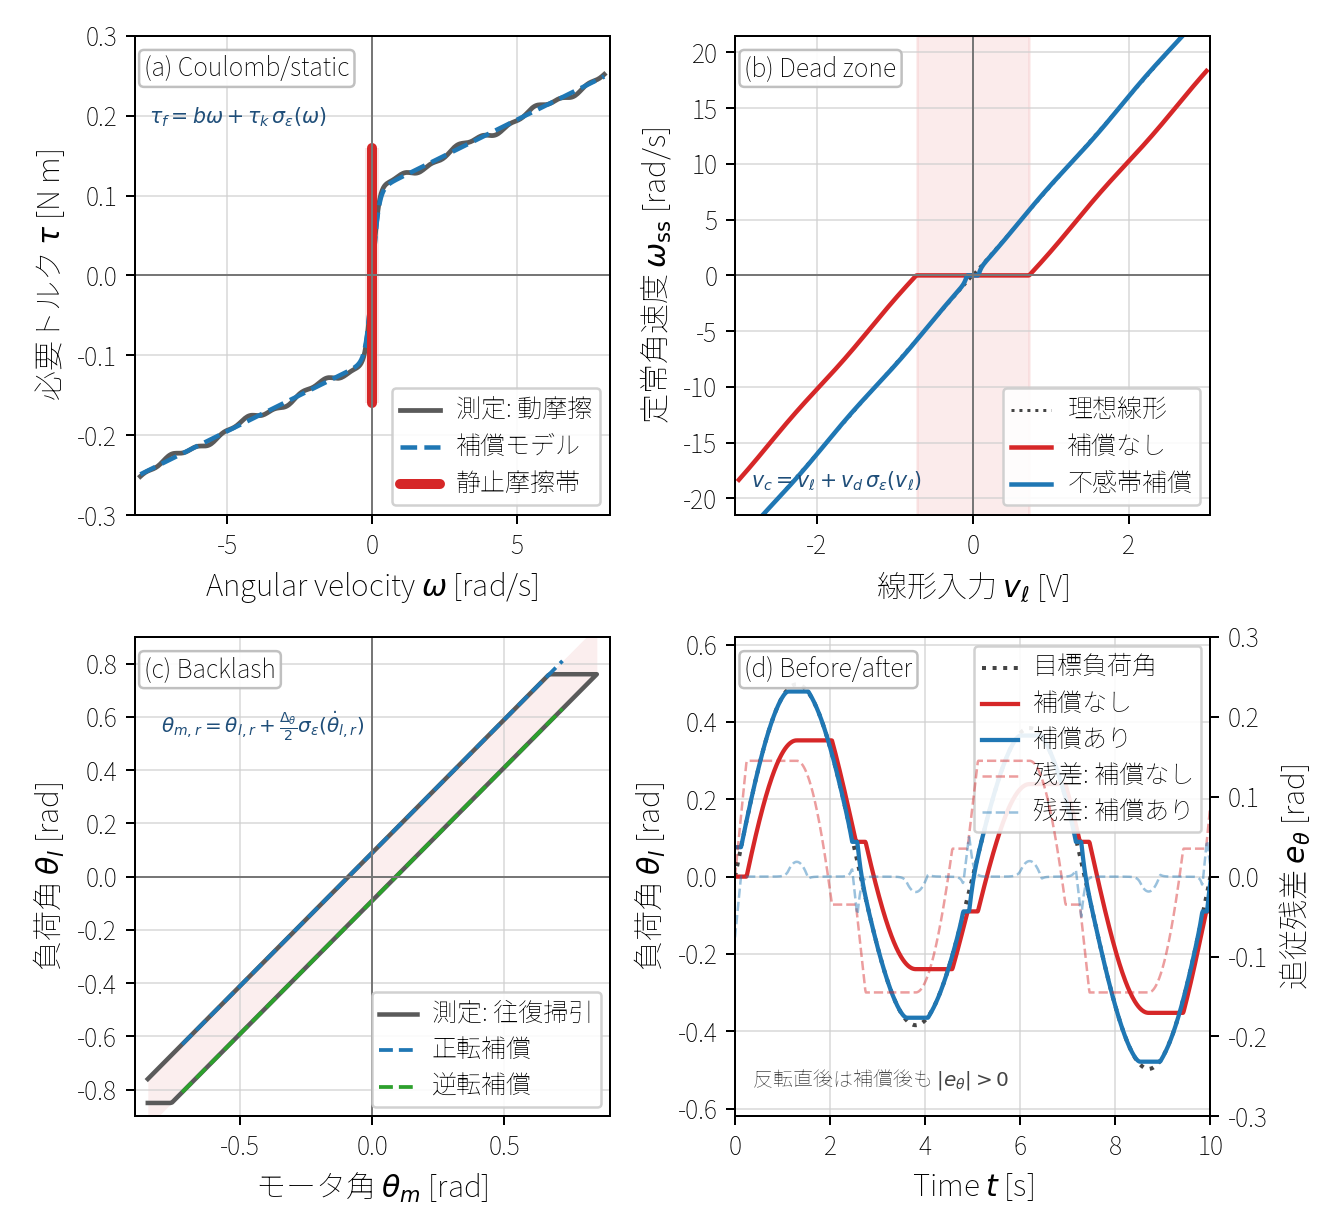
\includegraphics[width=0.96\linewidth,bb=0 0 1332 1224]{figures/friction_deadzone_backlash_examples.png}
\caption{摩擦・不感帯・バックラッシの低速測定曲線と補償例。左上は静止摩擦帯と Coulomb 摩擦を含む必要トルク、右上は不感帯を持つ電圧-角速度特性と逆向きの電圧補償、左下は往復掃引で得られるバックラッシ曲線と接触側を選ぶ角度補償、右下は反転を含む負荷角追従の補償前後である。補償後も反転直後の残差は残り、これはすきまを詰める時間と摩擦変動が残るためである。}
\label{fig:friction-deadzone-backlash-examples}
\end{figure}

\subsubsection{補償後に残る限界}

\wfig{friction-deadzone-backlash-examples} の右下では、不感帯とバックラッシを補償しない場合、目標負荷角が小さく変わっても出力が止まり、方向反転後に負荷側の動き出しが遅れている。
補償を入れると、小さな目標変化でも不感帯を越える入力が作られ、反転時にはモータ軸目標が先にずれるため、追従残差は小さくなる。
ただし、残差は 0 にはならない。
理由は三つある。

第一に、静止摩擦は荷重、温度、潤滑状態、停止時間で変わる。
測定値 $\tau_s$ を少し大きめに補償すると止まりにくくなるが、大きすぎると目標近傍で正負に入力が切り替わり、微小な往復運動を作る。
第二に、不感帯幅 $v_d$ はドライバ、電源電圧、PWM 分解能、機械抵抗によって変わる。
補償式の $v_d$ は一定値ではなく、実装では温度や速度範囲ごとに表を切り替える場合がある。
第三に、バックラッシは接触していない区間では負荷側の位置を拘束しない。
反転直後に幅 $\Delta_\theta$ のすきまを詰めるには、少なくとも
\[
  t_{\mathrm{takeup}}
  \gtrsim
  \frac{\Delta_\theta}{|\dot{\theta}_m|}
\]
の時間が必要である。
電圧制限や速度制限によって $|\dot{\theta}_m|$ が上げられないと、この遅れは補償式だけでは消えない。

したがって、摩擦・不感帯・バックラッシ補償は完全な相殺ではなく、測定した失われる入力範囲を先に越えるための前置補償である。
線形フィードバックは補償後にも必要であり、残る誤差、温度変化、モデル誤差、飽和時の切り詰めを吸収する役割を持つ。
次の段階で速度・加速度の目標値から単純なフィードフォワードを加えるときも、ここで扱った補償項と飽和条件を同時に見る必要がある。

\subsection{追従のためのフィードフォワード}

摩擦、不感帯、バックラッシュを補償しても、フィードバックだけで既知の速度や軌道を追う場合には一つの遅れが残る。フィードバックは、測定値が目標値からずれた後に操作量を増やす構造である。すでに分かっている目標速度、目標加速度、目標軌道の曲率、または測定済みの負荷外乱があるなら、それらを偏差が現れる前に操作量へ入れられる。この先回り入力がフィードフォワードである。

ここで扱うフィードフォワードは、フィードバックを置き換えるものではない。補償後の DC モータでも、名目慣性、粘性係数、トルク定数、車輪半径、路面状態は真値と完全には一致しない。したがって、既知の運動に必要な入力を先に入れ、残ったモデル誤差、初期値のずれ、未測定外乱、飽和の影響をフィードバックで戻す、という役割分担で使う。

\subsubsection{速度と加速度から作る DC モータの先回り電流}

前段までのカスケード制御では、電流ループが十分速い範囲で速度ループから見る入力を電流指令として扱った。摩擦補償後の速度軸を
\begin{equation}
  J\dot{\omega}+b\omega+\tau_f(\omega)+\tau_L=K_t i
  \label{eq:feedforward-motor-model}
\end{equation}
で表す。$\omega\,[\mathrm{rad/s}]$ は角速度、$i\,[\mathrm{A}]$ は電流、$J\,[\mathrm{kg\,m^2}]$ は慣性、$b\,[\mathrm{N\,m\,s/rad}]$ は粘性係数、$K_t\,[\mathrm{N\,m/A}]$ はトルク定数、$\tau_f$ は摩擦トルク、$\tau_L$ は負荷トルクである。前節の摩擦補償で $\tau_f$ の主要成分を入力側へ入れた後でも、目標角速度 $\omega_r(t)$ を急に変えると、加速に必要なトルク $J\dot{\omega}_r$ は偏差が出る前に必要になる。

名目値 $J_n,b_n,K_{t,n}$ と、必要なら目標速度上で評価した摩擦補償 $\hat{\tau}_{f,r}$ を使うと、速度・加速度フィードフォワード電流は
\begin{equation}
  i_{ff}
  =
  \frac{
    J_n\dot{\omega}_r
    +b_n\omega_r
    +\hat{\tau}_{f,r}
    +\tau_{L,m}
  }{K_{t,n}}
  \label{eq:speed-acceleration-feedforward}
\end{equation}
である。$\tau_{L,m}$ は測定された負荷トルクであり、測れない場合は 0 とおく。加速度項 $J_n\dot{\omega}_r/K_{t,n}$ は速度を変えるための電流、粘性項 $b_n\omega_r/K_{t,n}$ はその速度を保つための電流、負荷項 $\tau_{L,m}/K_{t,n}$ は測定済みの外乱を相殺する電流である。

実際の電流指令は、フィードフォワードだけでなく速度偏差も使って
\begin{align}
  e_\omega&=\omega_r-\omega,\\
  i_c&=i_{ff}+K_P e_\omega+K_I\int e_\omega\,dt,\\
  i&=\operatorname{sat}_{[-I_{\max},I_{\max}]}(i_c)
  \label{eq:feedforward-feedback-current}
\end{align}
とする。$K_P$ の単位は $\mathrm{A/(rad/s)}$、$K_I$ の単位は $\mathrm{A/rad}$ である。フィードフォワードが正しければ $e_\omega$ は小さくなり、フィードバックは大きな追従入力ではなく補正入力として働く。名目値がずれていれば、式 \eqref{eq:feedforward-feedback-current} の比例・積分項が残差を修正する。

\begin{figure}[tbp]
\centering
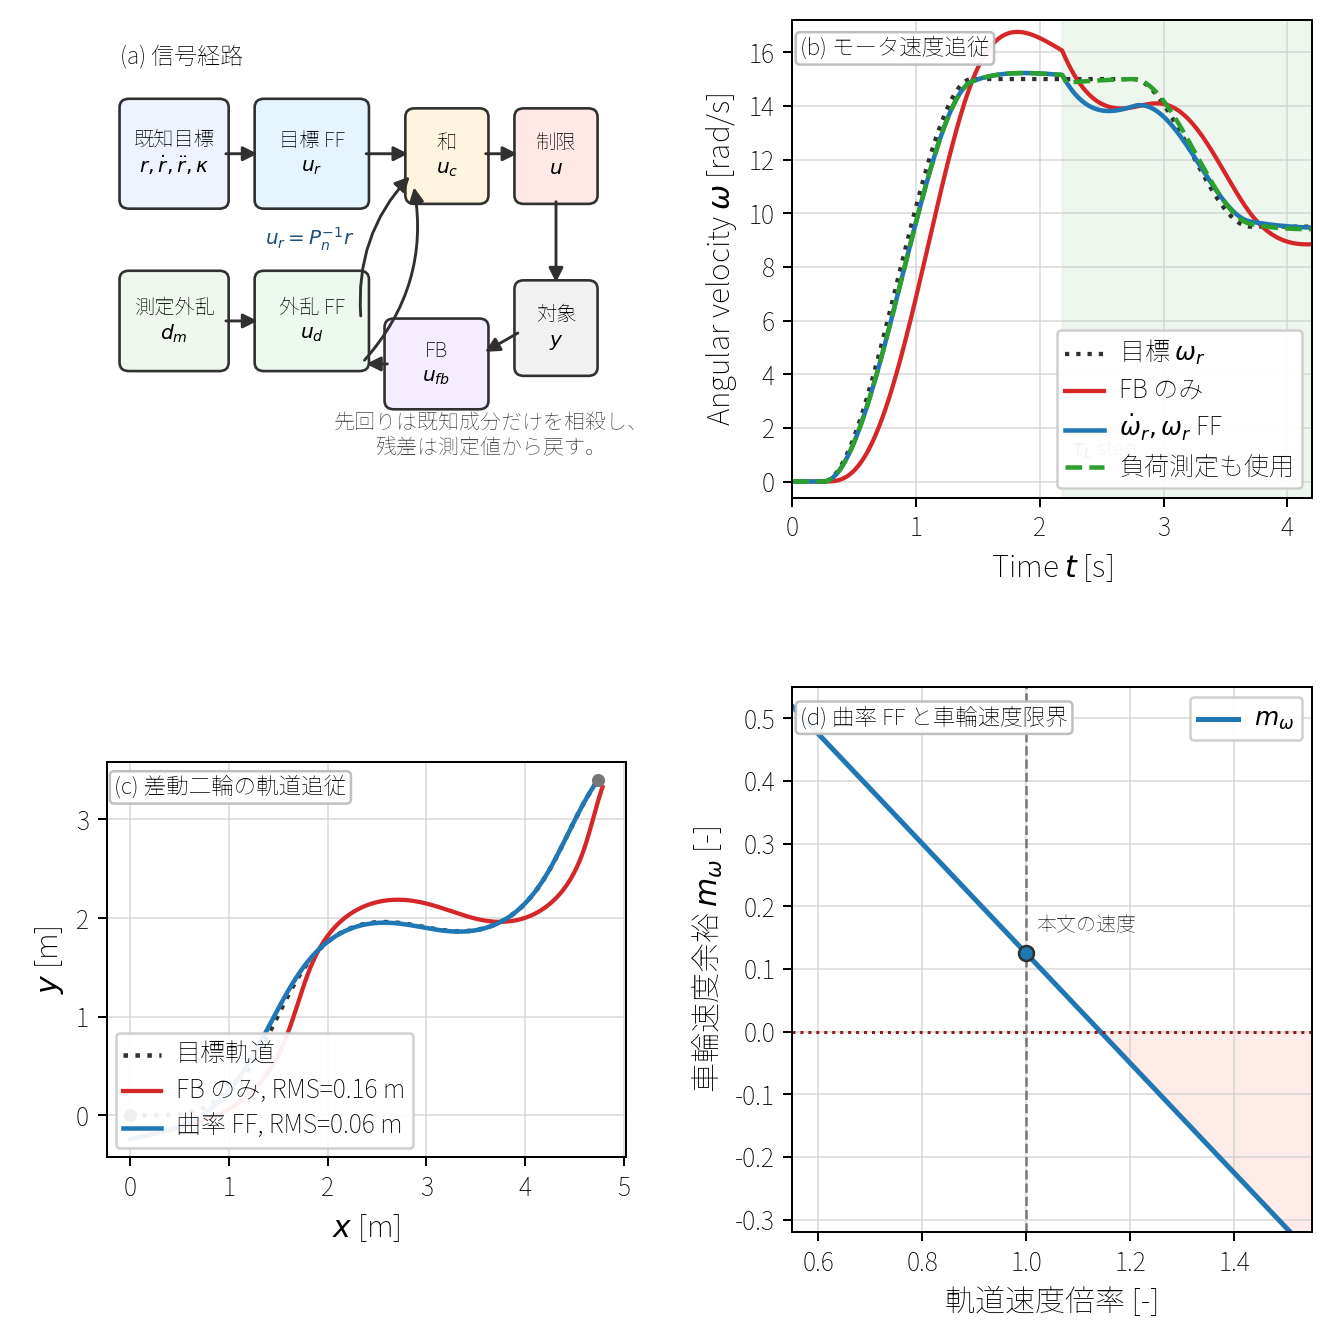
\includegraphics[width=0.98\linewidth,bb=0 0 1332 1332]{figures/feedforward_tracking_examples.png}
\caption{速度・加速度フィードフォワード、曲率フィードフォワード、測定外乱補償の役割。上段左は、既知目標と測定外乱から先回り入力を作り、残差をフィードバックで戻す信号経路である。上段右は DC モータ速度追従で、$\dot{\omega}_r$ と $\omega_r$ から作る電流を加えると立上り遅れが減り、負荷トルク測定 $\tau_{L,m}$ も使うと負荷投入後の速度低下がさらに小さくなる。下段左は差動二輪ロボットの軌道追従で、曲率フィードフォワードを入れると曲がり始めの横偏差が減る。下段右は軌道速度倍率を上げたときの車輪速度余裕 $m_\omega$ で、曲率が大きい軌道ほど外側車輪の上限が追従可能性を決める。}
\label{fig:feedforward-tracking-examples}
\end{figure}

\wfig{feedforward-tracking-examples} の上段右では、速度目標を滑らかに上げた後、$t=2.18\,\mathrm{s}$ で負荷トルクを加えている。フィードバックだけの場合は、目標が動き出してから速度偏差が増え、その偏差によって電流が増えるため、立上りで遅れる。式 \eqref{eq:speed-acceleration-feedforward} の速度・加速度項を入れると、加速に必要な電流が最初から出るので、追従誤差は小さくなる。さらに負荷トルクが測定できる場合は、$\tau_{L,m}/K_{t,n}$ を同じ電流指令に足すことで、負荷投入直後の速度低下を小さくできる。ただし図の緑線にも小さな残差がある。測定遅れ、名目値誤差、電流制限、摩擦補償の残りがあるため、測定外乱補償を入れてもフィードバックは必要である。

\subsubsection{差動二輪ロボットの曲率フィードフォワード}

速度フィードフォワードは一軸モータだけの考え方ではない。差動二輪ロボットでは、追いたい軌道の中心速度と曲率が分かっていれば、左右車輪がどの速度で回るべきかを偏差が出る前に計算できる。車輪半径を $r_w\,[\mathrm{m}]$、左右車輪間隔を $B\,[\mathrm{m}]$、車体中心の目標並進速度を $v_r(t)\,[\mathrm{m/s}]$、目標曲率を $\kappa_r(t)\,[1/\mathrm{m}]$ とする。曲率は弧長 $s$ に対する姿勢角 $\psi$ の変化率
\begin{equation}
  \kappa_r=\frac{d\psi_r}{ds}
  \label{eq:path-curvature-definition}
\end{equation}
であり、時間微分では
\begin{equation}
  \dot{\psi}_r
  =
  \frac{d\psi_r}{ds}\frac{ds}{dt}
  =
  \kappa_r v_r
  \label{eq:yaw-rate-curvature}
\end{equation}
となる。したがって、左右車輪の目標角速度は
\begin{align}
  \omega_{\mathrm{R},ff}
  &=
  \frac{
    v_r+\frac{B}{2}\dot{\psi}_r
  }{r_w}
  =
  \frac{
    v_r\left(1+\frac{B}{2}\kappa_r\right)
  }{r_w},\\
  \omega_{\mathrm{L},ff}
  &=
  \frac{
    v_r-\frac{B}{2}\dot{\psi}_r
  }{r_w}
  =
  \frac{
    v_r\left(1-\frac{B}{2}\kappa_r\right)
  }{r_w}.
  \label{eq:differential-drive-curvature-feedforward}
\end{align}
直線では $\kappa_r=0$ なので左右は同じ速度になる。左へ曲がる正の曲率では、右車輪が外側を通るため $\omega_{\mathrm{R},ff}$ が大きくなり、左車輪は小さくなる。

軌道追従では、式 \eqref{eq:differential-drive-curvature-feedforward} をそのまま出すだけでは初期位置ずれを戻せない。そこで、参照姿勢 $\psi_r$ の座標系で位置誤差を
\begin{align}
  e_x&=\cos\psi_r(x_r-x)+\sin\psi_r(y_r-y),\\
  e_y&=-\sin\psi_r(x_r-x)+\cos\psi_r(y_r-y),\\
  e_\psi&=\operatorname{wrap}(\psi_r-\psi)
  \label{eq:trajectory-error-frame}
\end{align}
と定義する。$e_x$ は軌道方向、$e_y$ は横方向、$e_\psi$ は向きの誤差である。簡単な追従則として
\begin{align}
  v_c&=v_r+k_xe_x,\\
  \dot{\psi}_c&=v_r\kappa_r+k_y e_y+k_\psi e_\psi
  \label{eq:curvature-feedforward-feedback-law}
\end{align}
を使う。第二式の先頭 $v_r\kappa_r$ が曲率フィードフォワードであり、残りの $k_y e_y+k_\psi e_\psi$ が横偏差と姿勢偏差を戻すフィードバックである。曲率項を抜くと、ロボットは曲がるべき場所に来ても直進を続け、横偏差または姿勢偏差が生じてから初めて旋回する。曲率項を入れると、目標軌道が曲がり始める時点で左右車輪速度が分かれ、フィードバックは初期ずれとモデル誤差の補正に回る。

\wfig{feedforward-tracking-examples} の下段左は、同じ初期ずれから始めた差動二輪ロボットの比較である。赤線のフィードバックのみでは、曲率が変わるたびに横偏差が先に発生し、その後に向きが戻る。青線の曲率フィードフォワードでは、式 \eqref{eq:differential-drive-curvature-feedforward} により外側車輪と内側車輪の速度差が先に作られるため、同じフィードバックゲインでも軌道中心に近いまま曲がれる。

\subsubsection{逆モデルフィードフォワードの範囲と限界}

速度・加速度項も曲率項も、広い意味では「望む出力から必要入力を逆に計算する」処理である。線形対象を
\begin{equation}
  y=P(s)u+P_d(s)d
  \label{eq:inverse-model-feedforward-plant}
\end{equation}
と書き、名目モデルを $P_n(s),P_{d,n}(s)$ とする。目標値 $r$ に対して名目上 $y=r$ を満たしたいなら、形式的には
\begin{equation}
  u_r=P_n^{-1}(s)r
  \label{eq:nominal-inverse-reference-feedforward}
\end{equation}
である。測定外乱 $d_m$ がある場合は、外乱から出力までの影響を打ち消すように
\begin{equation}
  u_d=-P_n^{-1}(s)P_{d,n}(s)d_m
  \label{eq:measured-disturbance-feedforward}
\end{equation}
を加える。モータ負荷トルクの例では、$d_m=\tau_{L,m}$、$u_d=\tau_{L,m}/K_{t,n}$ であり、式 \eqref{eq:speed-acceleration-feedforward} の負荷項に対応する。

しかし、式 \eqref{eq:nominal-inverse-reference-feedforward} と式 \eqref{eq:measured-disturbance-feedforward} はそのまま使えるとは限らない。第一に、$P_n^{-1}$ がプロパーで安定でなければ、微分を過剰に要求したり、右半平面零点やむだ時間を不安定な逆として反転したりする。第二に、モデルが合っていても入力制限がある。\wfig{feedforward-tracking-examples} の下段右では、車輪速度余裕を
\begin{equation}
  m_\omega
  =
  1-
  \frac{
    \max(|\omega_{\mathrm{L},c}|,|\omega_{\mathrm{R},c}|)
  }{\Omega_{\max}}
  \label{eq:wheel-speed-margin-feedforward}
\end{equation}
で評価している。$m_\omega>0$ なら左右車輪指令は上限 $\Omega_{\max}$ の内側にあり、$m_\omega<0$ なら曲率フィードフォワードが要求する車輪速度を実機が出せない。軌道速度倍率を上げると $v_r$ と $\dot{\psi}_r=v_r\kappa_r$ が同時に増えるため、外側車輪の余裕が先に消える。

第三に、測定外乱補償は測定できる成分だけを相殺する。負荷トルク計が遅れを持つ場合、床面の傾きや摩擦変化を測っていない場合、または外乱の作用点を名目モデルが誤っている場合、式 \eqref{eq:measured-disturbance-feedforward} の相殺は完全ではない。測定値にノイズがあると、外乱フィードフォワード自体が入力ノイズになることもある。

このため、実装上の構成は
\begin{equation}
  u
  =
  \operatorname{sat}
  \left(
    u_r+u_d+u_{fb}
  \right),
  \qquad
  u_{fb}=C(r-y)
  \label{eq:feedforward-feedback-implementation}
\end{equation}
である。$u_r$ は既知目標の先回り入力、$u_d$ は測定外乱の先回り補償、$u_{fb}$ は残差を戻す入力である。フィードフォワードを入れるほど、フィードバックが修正する誤差は小さくできるが、フィードバックをなくすと、初期ずれ、モデル誤差、未測定外乱、飽和後の入力不足を戻す経路がなくなる。したがって、ここでの結論は、フィードフォワードで「予測できる入力」を先に払い、フィードバックで「予測できなかった差」を測定から戻す、という分担である。この分担を信頼するためには、次に名目モデルがどの程度実機に合っているかを同定とモデル検証で評価する必要がある。

\subsection{同定と検証残差から見た補償の限界}

逆モデルやモデルベースフィードフォワードは、目標速度や既知外乱から必要入力を先に計算できるため、フィードバックだけに頼る場合より偏差を小さくできる。しかし、その計算はモデルを信じる操作でもある。DC モータ速度制御で
\begin{equation}
  \tau_n\dot{\omega}+\omega=K_n v
\end{equation}
という名目モデルを置くと、望ましい速度 $\omega_r(t)$ に対する単純な逆モデルフィードフォワードは
\begin{equation}
  v_{ff}(t)
  =
  \frac{\tau_n\dot{\omega}_r(t)+\omega_r(t)}{K_n}
  \label{eq:identified-inverse-feedforward}
\end{equation}
である。ここで $v$ は入力電圧 $[\mathrm{V}]$、$\omega$ は角速度 $[\mathrm{rad/s}]$、$K_n$ は定常ゲイン $[\mathrm{rad/s/V}]$、$\tau_n$ は時定数 $[\mathrm{s}]$ である。$K_n$ が実機より大きく見積もられていれば必要電圧は小さく計算され、加速不足が残る。$\tau_n$ が実機より小さければ、加速に必要な電圧を過小評価する。静止摩擦、デッドゾーン、負荷トルク、電圧飽和が入ると、式 \eqref{eq:identified-inverse-feedforward} の誤差はさらに大きくなる。

したがって、モデルベース補償を使う前に、実測データでモデルを同定し、別のデータで検証する必要がある。同定は「係数をもっともらしく決める」作業であり、検証は「その係数で、まだ見ていない運転条件をどの程度予測できるか」を測る作業である。補償の主張は、検証残差より細かくはならない。検証データで $1\,\mathrm{rad/s}$ 程度の予測誤差が残っているモデルを使って、フィードフォワードだけで $0.1\,\mathrm{rad/s}$ の追従精度を保証することはできない。

\subsubsection{同定用データと検証用データの分離}

まず、モータに複数の電圧レベルを与え、入力 $v_k$ と速度測定値 $\omega_k$ をサンプリング周期 $T_s$ ごとに記録する。電圧は正負の両側を含み、速度が上がる区間、下がる区間、低速でデッドゾーンの影響を受ける区間を含める。一定電圧を一つだけ入れたデータでは、時定数とゲイン、バイアス、摩擦を分けて読み取れない。

ここでは連続時間の一次モデル
\begin{equation}
  \tau\dot{\omega}+\omega=Kv+\omega_b
  \label{eq:identification-first-order-model}
\end{equation}
を、サンプル値の近似モデル
\begin{equation}
  \omega_{k+1}
  =
  a\omega_k+bv_k+c+\varepsilon_k
  \label{eq:identification-discrete-first-order}
\end{equation}
として当てはめる。$\varepsilon_k$ は、測定ノイズ、未測定外乱、モデルに入れていない摩擦やデッドゾーンの影響をまとめた残差である。式 \eqref{eq:identification-discrete-first-order} で $0<a<1$ なら、連続時間の時定数とゲインは
\begin{equation}
  \hat{\tau}
  =
  -\frac{T_s}{\log \hat{a}},
  \qquad
  \hat{K}
  =
  \frac{\hat{b}}{1-\hat{a}}
  \label{eq:identification-continuous-parameters}
\end{equation}
へ戻せる。$c$ は平衡点のずれや低速摩擦を一次モデルの中で吸収する項であり、理想的な線形モータでは 0 に近い。

同定では、データ全体を一度に使わず、前半を同定用、後半を検証用に分ける。時刻 $t_k$ が $0.4\,\mathrm{s}$ から $8.0\,\mathrm{s}$ までのサンプルを同定用集合 $\mathcal{D}_{id}$ とし、それ以降を検証用集合 $\mathcal{D}_{val}$ とする。各サンプルについて
\begin{equation}
  \phi_k=
  \begin{bmatrix}
    \omega_k\\
    v_k\\
    1
  \end{bmatrix},
  \qquad
  \theta=
  \begin{bmatrix}
    a\\
    b\\
    c
  \end{bmatrix}
\end{equation}
と置くと、予測式は $\omega_{k+1}=\phi_k^\T \theta+\varepsilon_k$ である。同定用データに対する二乗残差和
\begin{equation}
  J_{id}(\theta)
  =
  \sum_{k\in\mathcal{D}_{id}}
  \left(\omega_{k+1}-\phi_k^\T \theta\right)^2
  \label{eq:identification-least-squares-cost}
\end{equation}
を最小にする係数は、正規方程式から
\begin{align}
  0
  &=
  \frac{\partial J_{id}}{\partial \theta}
  =
  -2\sum_{k\in\mathcal{D}_{id}}
  \phi_k\left(\omega_{k+1}-\phi_k^\T \theta\right),\\
  \left(\sum_{k\in\mathcal{D}_{id}}\phi_k\phi_k^\T\right)\hat{\theta}
  &=
  \sum_{k\in\mathcal{D}_{id}}\phi_k\omega_{k+1},\\
  \hat{\theta}
  &=
  \left(\sum_{k\in\mathcal{D}_{id}}\phi_k\phi_k^\T\right)^{-1}
  \sum_{k\in\mathcal{D}_{id}}\phi_k\omega_{k+1}
  \label{eq:identification-normal-equation}
\end{align}
で与えられる。ただし、括弧内の行列が逆行列を持つには、入力と速度が十分に変化し、$\omega_k$、$v_k$、定数項の情報が同じ向きに偏りすぎていないことが必要である。

\begin{figure}[tbp]
\centering
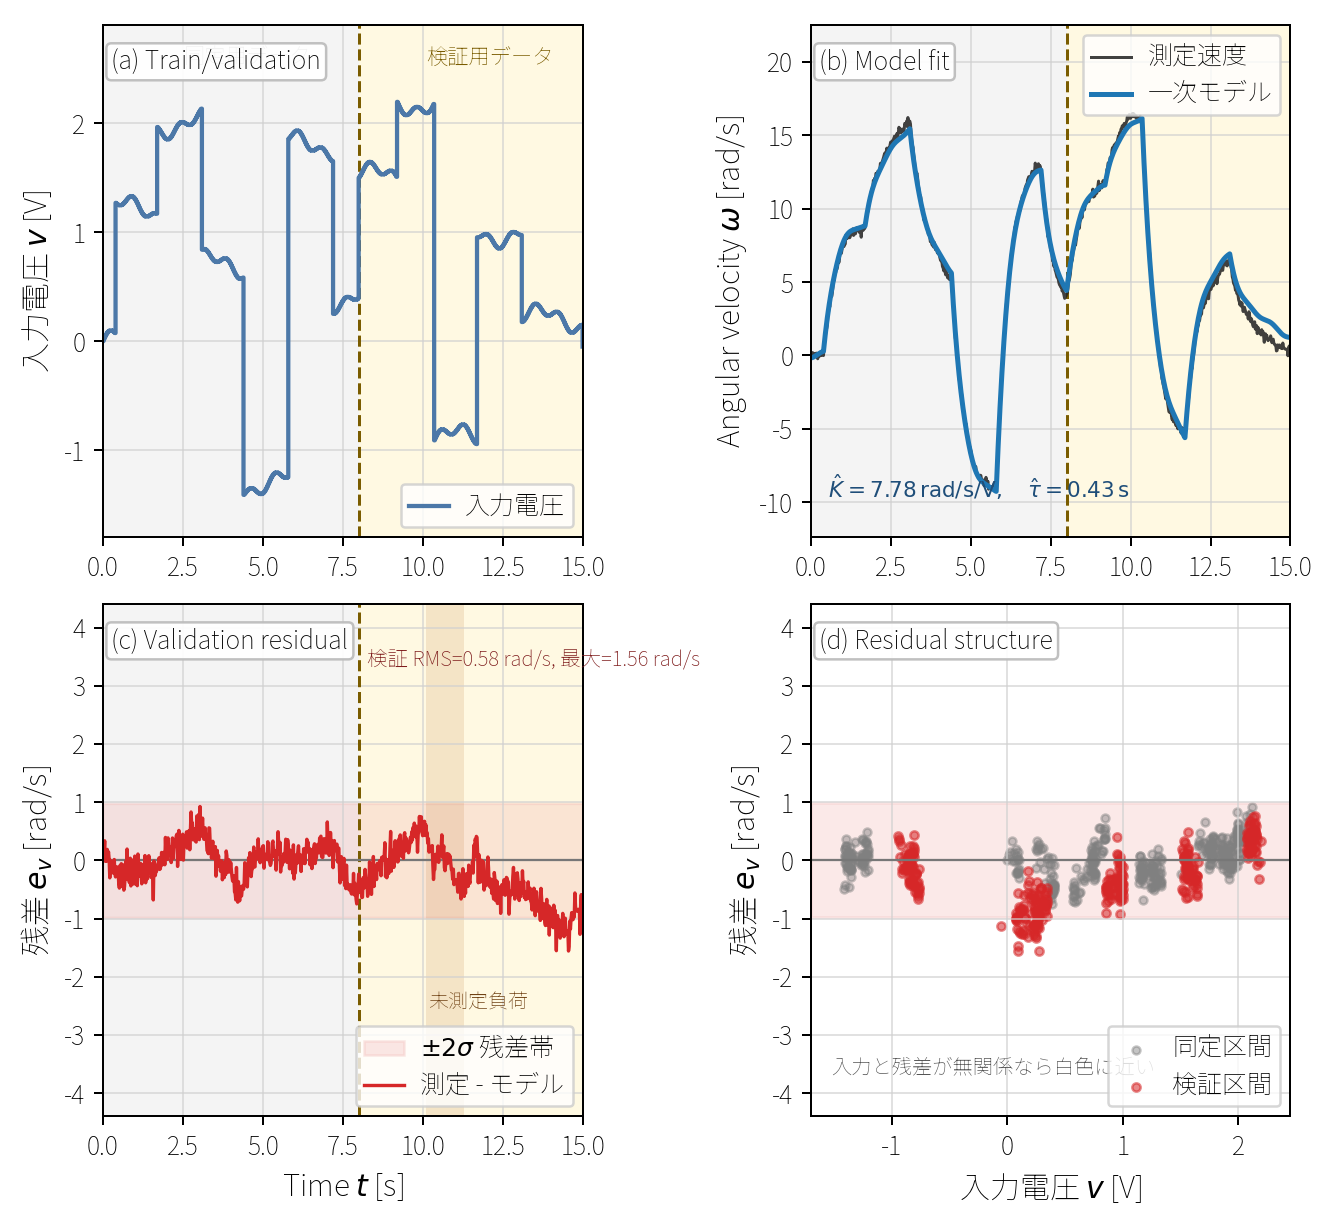
\includegraphics[width=0.98\linewidth,bb=0 0 1332 1224]{figures/identification_residual_examples.png}
\caption{DC モータ速度応答の一次モデル同定と検証残差。上段左は入力電圧の時系列で、灰色を同定用データ、淡い黄色を検証用データとした。上段右は同定用データから得た $\hat{K}=7.78\,\mathrm{rad/s/V}$、$\hat{\tau}=0.43\,\mathrm{s}$ の一次モデルを全区間へ適用した結果である。下段左は測定速度とモデル予測の差であり、検証区間の RMS 残差は $0.58\,\mathrm{rad/s}$、最大絶対残差は $1.56\,\mathrm{rad/s}$ である。下段右は入力電圧と残差の関係を表し、残差が入力や検証区間に依存している部分が未モデル化要素を表す。}
\label{fig:identification-residual-examples}
\end{figure}

\wfig{identification-residual-examples} は、サンプリング周期 $T_s=0.02\,\mathrm{s}$ で記録した速度データに、式 \eqref{eq:identification-discrete-first-order} を当てはめた例である。同定用データだけを見ると、測定速度とモデル速度はよく重なっている。推定値は $\hat{K}=7.78\,\mathrm{rad/s/V}$、$\hat{\tau}=0.43\,\mathrm{s}$ であり、少なくとも同じ範囲の電圧変化に対しては、一次遅れ近似として使える。

重要なのは、同定に使っていない検証区間で残差を読むことである。検証残差を
\begin{equation}
  e_{v,k}
  =
  \omega_k-\hat{\omega}_k
  \label{eq:validation-residual}
\end{equation}
と定義する。ここで $\hat{\omega}_k$ は、推定した係数を固定したまま、実際の入力電圧列を入れて計算したモデル速度である。図の検証区間では
\begin{equation}
  e_{rms}
  =
  \sqrt{
  \frac{1}{N_{val}}
  \sum_{k\in\mathcal{D}_{val}}e_{v,k}^2
  }
  =
  0.58\,\mathrm{rad/s},
  \qquad
  \max_{k\in\mathcal{D}_{val}}|e_{v,k}|
  =
  1.56\,\mathrm{rad/s}
  \label{eq:validation-residual-values}
\end{equation}
となっている。下段左の $10.1$ から $11.3\,\mathrm{s}$ 付近では、未測定負荷を入れたため残差が偏る。下段右では、検証区間の残差が入力電圧の値によってまとまっており、残差が単なる白色測定ノイズだけではないことが分かる。この構造は、デッドゾーン、速度依存ゲイン、負荷トルク、温度による抵抗変化などが一次モデルから漏れていることを意味する。

\subsubsection{残差がフィードフォワードの主張を制限する}

同定したモデルを式 \eqref{eq:identified-inverse-feedforward} に入れると、速度目標から電圧を先回り計算できる。しかし、検証残差が残っているなら、フィードフォワード後の誤差もその残差の範囲を基準に読まなければならない。一次モデルの予測誤差を連続時間で
\begin{equation}
  \tau\dot{\omega}+\omega=Kv+w_m(t)
  \label{eq:model-error-as-disturbance}
\end{equation}
と表すと、$w_m$ はモデル誤差を出力側へ換算した信号である。名目逆モデルで $v_{ff}$ を作っても、実機には
\begin{equation}
  \tau\dot{\omega}+\omega
  =
  K v_{ff}+w_m(t)
\end{equation}
が残る。$\tau$ と $K$ が名目値とずれ、さらに $w_m$ が検証残差として現れているなら、開ループのフィードフォワードだけではその成分を消せない。フィードバックは、この残差、未知外乱、初期値ずれを測定偏差として受け取り、安定余裕と入力制約の範囲で修正する役割を持つ。

残差は、補償の設計範囲を決める実験的な境界でもある。図の例では、同じ電圧範囲と同じ温度条件で検証したとき、RMS 残差は $0.58\,\mathrm{rad/s}$ である。したがって、このモデルを使った速度フィードフォワードは、少なくとも同程度の速度誤差が残る可能性を前提に置く。制御仕様として定常速度誤差を $0.2\,\mathrm{rad/s}$ 以下にしたいなら、一次モデルだけでは根拠が足りない。摩擦やデッドゾーンを別に同定する、負荷トルクを測る、フィードバック帯域を上げる、参照値を遅くして飽和を避ける、といった追加の根拠が必要になる。

また、残差がランダムに散らばらず、入力電圧、速度、回転方向、温度、時間に依存して偏る場合は、平均値を 0 に近づけただけでは不十分である。残差が入力電圧に依存しているなら、ゲインが一定でない。残差が速度の符号で変わるなら、摩擦やデッドゾーンが残っている。残差が特定時刻で偏るなら、未測定負荷や電源電圧の変動が入っている。残差が高周波に多いなら、センサノイズやサンプリング遅れを逆モデルが増幅している。これらの構造を見ずに、二乗誤差の平均だけで「モデルはよい」と判断すると、補償が効く範囲を過大評価する。

\subsubsection{補償後に残るロバスト性限界}

ここまでの流れでは、飽和に対してアンチワインドアップを入れ、参照値を整形し、カスケード制御で内部量を速く制御し、摩擦やデッドゾーンを補償し、さらにモデルベースフィードフォワードで必要入力を先に与えた。それでも制御系が完全になるわけではない。残る限界は、少なくとも次の五つに分けられる。

第一に、モデル誤差である。同定した一次モデルは、同定データの範囲で平均的に合う近似であり、すべての速度、温度、負荷、電源電圧、摩耗状態で正しい物理式ではない。検証残差が入力や時刻に依存しているなら、その依存性はフィードフォワード後にも残る。必要なら、速度依存ゲイン、摩擦項、デッドゾーン、むだ時間、電圧飽和をモデルに加え、追加した項ごとに別の検証データで残差が本当に減ったかを確認する。

第二に、未測定外乱である。負荷トルクや路面抵抗が測定できる場合は外乱フィードフォワードで先に補える。しかし、測れていない外乱、遅れて届く外乱、符号や単位がずれた外乱は残差として現れる。外乱補償の効果は、外乱測定の帯域、遅れ、ノイズ、取り付け位置に制限される。

第三に、測定ノイズである。同定ではノイズが係数推定を揺らし、検証では残差の下限を作る。逆モデルや微分を含むフィードフォワードは高周波ノイズを大きくしやすい。したがって、速度や加速度を使う補償では、フィルタの遅れとノイズ低減を同時に見なければならない。ノイズを完全に消そうとしてフィルタを遅くしすぎると、今度は補償入力が実際の運動から遅れる。

第四に、飽和とレート制限である。モデルが正しくても、式 \eqref{eq:identified-inverse-feedforward} が電圧、電流、トルク、速度、温度の制約を越える入力を出すなら、その入力は実機へ入らない。飽和後の入力で動く実機は、同定に使った線形モデルとは別の非線形系になる。したがって、同定残差が小さいことと、要求入力が実現可能であることは別々に確認する必要がある。

第五に、推定値の不確かさである。$\hat{K}$ と $\hat{\tau}$ は有限のデータから得た値であり、入力波形、測定ノイズ、サンプリング周期、運転条件に依存する。別の日、別の温度、別の負荷では推定値が変わる。実装では、係数を一点の値として扱うだけでなく、検証残差と係数のばらつきから余裕を残す。たとえば、フィードフォワード入力を少し控えめにし、フィードバックで残差を吸収し、残差が増えたときには補償を弱める監視を入れる。

この段階で得られる結論は、モデルベース補償を捨てることではない。むしろ、モデルを使う範囲を実測で区切ることで、フィードフォワードとフィードバックの役割分担が明確になる。フィードフォワードは、検証された帯域と入力範囲で既知の運動や既知外乱を先に補う。フィードバックは、検証残差、未知外乱、ノイズ、飽和、係数ずれを受け止める。次に性能指標を導入するときは、追従誤差だけでなく、RMS 入力、ピーク入力、制約余裕、残差の大きさを同時に数値化し、手調整でどこまで改善でき、どこから複数目的の重み付けが必要になるかを評価する。

\subsection{性能指標と Pareto 図による手調整の数値化}

同定、フィードフォワード、外乱補償、摩擦や不感帯の補償を順に入れても、実機の応答には残差が残る。残差が残った段階で、候補 A は少し速い、候補 B は入力が小さい、候補 C は余裕がある、という言い方だけで調整を続けると、どの改善をどの悪化で買っているのかが曖昧になる。ここで必要になるのは、手調整の候補を同じ測定時間、同じ目標値、同じ入力制約で数値化する基準である。

直前までの DC モータサーボの話とつなげるため、ここでは角度 $\theta(t)\,[\mathrm{rad}]$、角速度 $\omega(t)\,[\mathrm{rad/s}]$、入力電圧 $u(t)\,[\mathrm{V}]$ の低次モデルを使う。
\begin{align}
  \dot{\theta}&=\omega,\\
  J\dot{\omega}&=K_tu-b\omega,\\
  u&=\operatorname{sat}_{[-u_{\max},u_{\max}]}(u_c),\\
  u_c&=K_P(r-\theta)-K_D\omega .
  \label{eq:performance-motor-model}
\end{align}
ここで $J=0.20\,\mathrm{kg\,m^2}$、$b=0.25\,\mathrm{N\,m\,s/rad}$、$K_t=1.0\,\mathrm{N\,m/V}$、$u_{\max}=6.0\,\mathrm{V}$、目標値 $r=1.0\,\mathrm{rad}$ とする。積分器は入れない。位置目標を一定に保つと定常状態では $\omega=0$、$u=0$、$\theta=r$ が平衡になるので、この例では比例項と速度フィードバックだけでも定常偏差は消える。したがって、ここで比べたい主な差は、過渡応答の速さ、振動、入力要求、制約余裕である。

\subsubsection{時間波形から計算する性能指標}

シミュレーションまたは実測で、時刻 $t_k=k\Delta t$ の列
\begin{equation}
  \theta_k=\theta(t_k),\qquad
  u_{c,k}=u_c(t_k),\qquad
  e_k=r-\theta_k
\end{equation}
が得られているとする。評価時間は $0\leq t\leq T$ とし、ここでは $T=5.0\,\mathrm{s}$ である。積分は台形則
\begin{equation}
  \int_0^T f(t)\,dt
  \simeq
  \sum_{k=0}^{N-1}
  \frac{f_k+f_{k+1}}{2}\Delta t
  \label{eq:performance-trapezoid}
\end{equation}
で計算する。

整定時間は、応答が最後まで許容帯の中に残る最初の時刻で定義する。許容帯を $\varepsilon=0.02|r|$ とすると、
\begin{equation}
  t_s=
  \min\left\{
  t_i\ \middle|
  |e_j|\leq \varepsilon
  \text{ for all } j\geq i
  \right\}
  \label{eq:settling-time-definition}
\end{equation}
である。この定義では、一度 2\% 帯に入っても後で外へ出るなら、その時刻は整定とは数えない。

オーバーシュートは、目標値をどれだけ超えたかを百分率で表す。
\begin{equation}
  M_p=
  100
  \max\left(
  0,\frac{\max_k\theta_k-r}{|r|}
  \right)\,[\%].
  \label{eq:overshoot-definition}
\end{equation}
振動が大きい応答では、$t_s$ と $M_p$ の両方が悪化しやすい。ただし、行き過ぎが小さくても、ゆっくり尾を引く応答では $t_s$ が大きくなるため、二つは同じ情報ではない。

偏差の面積を測る指標として、IAE、ISE、ITAE を使う。
\begin{align}
  \mathrm{IAE}
  &=\int_0^T |e(t)|\,dt,\\
  \mathrm{ISE}
  &=\int_0^T e^2(t)\,dt,\\
  \mathrm{ITAE}
  &=\int_0^T t\,|e(t)|\,dt .
  \label{eq:error-integral-indices}
\end{align}
IAE は偏差の絶対量をそのまま積む。ISE は大きな偏差を二乗で強く罰する。ITAE は時間 $t$ を掛けるので、初期に少し大きな偏差がある応答より、後半まで小さな偏差を残す応答を重く罰する。単位も異なる。$\theta$ の単位が $\mathrm{rad}$ なら、IAE は $\mathrm{rad\,s}$、ISE は $\mathrm{rad^2\,s}$、ITAE は $\mathrm{rad\,s^2}$ である。

入力側の指標は、ここでは飽和前の計算入力 $u_c$ に対して定義する。
\begin{align}
  U_{\mathrm{rms}}
  &=
  \sqrt{\frac{1}{T}\int_0^T u_c^2(t)\,dt},\\
  U_{\mathrm{pk}}
  &=\max_k |u_{c,k}|,\\
  \mu_{\min}
  &=
  1-\frac{U_{\mathrm{pk}}}{u_{\max}} .
  \label{eq:input-indices-margin}
\end{align}
$U_{\mathrm{rms}}$ は平均的な入力要求、$U_{\mathrm{pk}}$ は瞬間的な最大要求である。$\mu_{\min}$ は制約余裕で、正なら全時刻で飽和前入力が制約内、0 ならちょうど上限、負なら制御器が物理的に出せない入力を要求していることを表す。実際の対象へ入る $u$ は飽和器で制限されるが、$u_c$ を見ないと「候補が本当はどれだけ無理を要求したか」を読めない。

\subsubsection{四つの候補の数値比較}

\wfig{performance-pareto-examples} は、式 \weq{performance-motor-model} に対して四つの PD 候補を同じ条件で計算した結果である。候補は
\begin{equation}
  \begin{array}{c|cc}
  \text{候補} & K_P & K_D\\ \hline
  \text{穏やか} & 2.0 & 1.10\\
  \text{低減衰} & 4.0 & 0.15\\
  \text{釣合い} & 4.0 & 0.90\\
  \text{強引} & 7.5 & 1.15
  \end{array}
\end{equation}
である。上段左の 2\% 帯を見ると、穏やかな候補は行き過ぎを出さないが、立上りが遅い。低減衰の候補は $K_P=4.0$ に対して $K_D$ が小さいため、大きく行き過ぎてから戻る。釣合いの候補は同じ $K_P=4.0$ のまま $K_D$ を増やしただけだが、速度フィードバックが減衰を増やすため、行き過ぎと後半の偏差が同時に小さくなる。強引な候補は最も速く見えるが、上段右で最初の $u_c$ が $6\,\mathrm{V}$ の上限を越えている。

\begin{figure}[tbp]
\centering
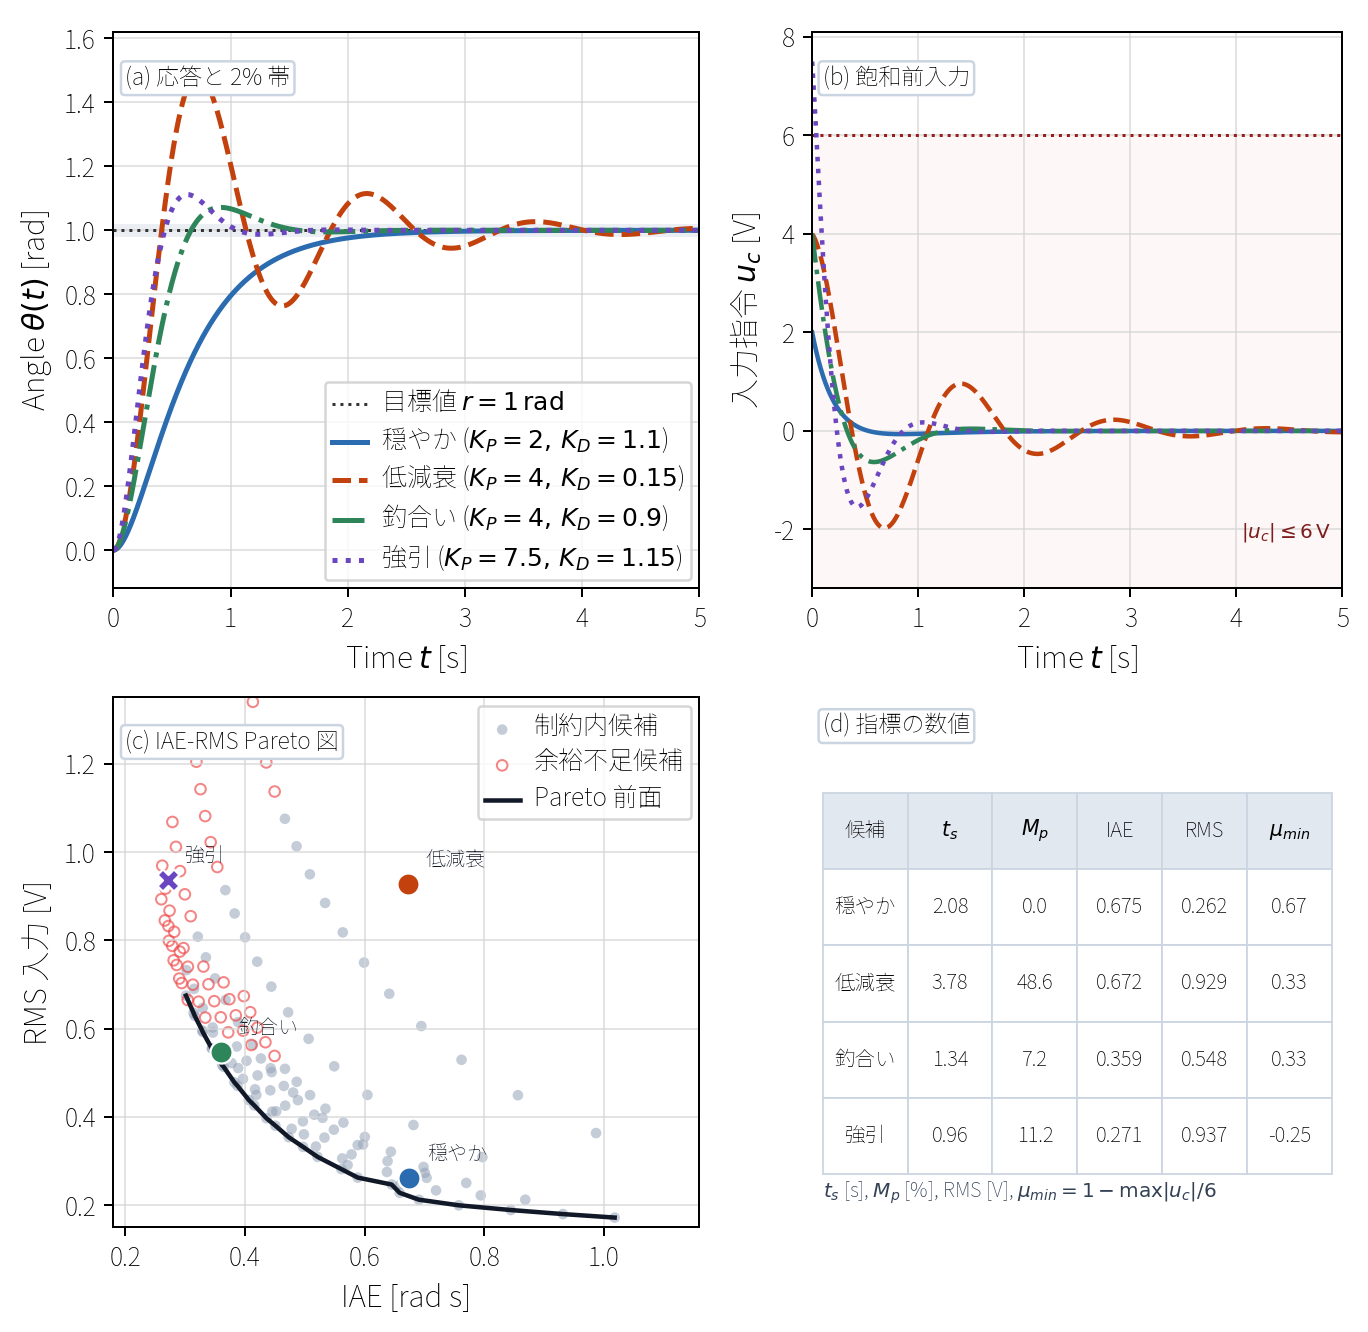
\includegraphics[width=0.98\linewidth,bb=0 0 1368 1332]{figures/performance_pareto_examples.png}
\caption{DC モータ位置サーボに対する性能指標と Pareto 図。対象は $J=0.20\,\mathrm{kg\,m^2}$、$b=0.25\,\mathrm{N\,m\,s/rad}$、$K_t=1.0\,\mathrm{N\,m/V}$、入力制約は $|u|\leq6.0\,\mathrm{V}$、目標値は $r=1.0\,\mathrm{rad}$ である。上段は応答と飽和前入力、下段左は多数の $K_P,K_D$ 候補を IAE と RMS 入力で比べた Pareto 図、下段右は代表候補の指標表である。}
\label{fig:performance-pareto-examples}
\end{figure}

同じ結果を数値表にすると、波形だけでは見落としやすい差がはっきりする。評価時間は $T=5.0\,\mathrm{s}$、整定帯は目標値の $2\%$ とした。$U_{\mathrm{rms}}$、$U_{\mathrm{pk}}$、$\mu_{\min}$ は飽和前入力 $u_c$ から計算している。
\begin{table}[tbp]
\centering
\caption{PD 候補の性能指標}
\label{tab:performance-indices-pareto}
\begingroup
\small
\setlength{\tabcolsep}{3pt}
\begin{tabular}{c|ccrrrrrr}
\hline
候補 & $t_s$ [s] & $M_p$ [\%] & IAE & ISE & ITAE & $U_{\mathrm{rms}}$ [V] & $U_{\mathrm{pk}}$ [V] & $\mu_{\min}$\\
\hline
穏やか & 2.08 & 0.0 & 0.675 & 0.412 & 0.356 & 0.262 & 2.00 & 0.67\\
低減衰 & 3.78 & 48.6 & 0.672 & 0.300 & 0.621 & 0.929 & 4.00 & 0.33\\
釣合い & 1.34 & 7.2 & 0.359 & 0.231 & 0.106 & 0.548 & 4.00 & 0.33\\
強引 & 0.96 & 11.2 & 0.271 & 0.169 & 0.066 & 0.937 & 7.50 & -0.25\\
\hline
\end{tabular}
\endgroup
\end{table}

低減衰の候補は、穏やかな候補と IAE がほぼ同じであるにもかかわらず、オーバーシュートは $48.6\%$、ITAE は $0.621$、RMS 入力は $0.929\,\mathrm{V}$ まで増えている。つまり、初期には速く動くが、後半まで振動が残るため、時間重み付きの偏差と入力要求の両方で不利になる。釣合いの候補は低減衰の候補と同じ $U_{\mathrm{pk}}=4.00\,\mathrm{V}$ で、制約余裕も同じ $0.33$ である。それでも $K_D$ を増やして減衰を足すだけで、$t_s$ は $3.78\,\mathrm{s}$ から $1.34\,\mathrm{s}$ へ短くなり、ITAE は $0.621$ から $0.106$ へ下がる。この比較では、低減衰の候補は釣合いの候補に支配されている。

強引な候補は IAE、ISE、ITAE のすべてが最小で、整定時間も $0.96\,\mathrm{s}$ と最短である。しかし $U_{\mathrm{pk}}=7.50\,\mathrm{V}$ であり、$\mu_{\min}=-0.25$ である。これは、制御器が上限の $1.25$ 倍の電圧を要求したことを意味する。飽和器を通した実入力は $6.0\,\mathrm{V}$ に制限されるので、表の速さは「入力制約を無視してよい」という結論ではない。むしろ、制約余裕を指標に入れないと、物理的に無理な候補を最良に見せてしまうことを示している。

\subsubsection{Pareto 図とスカラー評価への接続}

複数の指標を同時に小さくしたいとき、まず支配される候補を落とす。候補 $a$ と $b$ を IAE と RMS 入力で比べ、$a$ の IAE が $b$ 以下で、かつ $a$ の RMS 入力も $b$ 以下であり、少なくとも一方が厳密に小さいなら、$a$ は $b$ を支配する。このとき $b$ を選ぶ理由は、少なくともこの二つの指標だけからはない。

\wfig{performance-pareto-examples} の下段左は、$K_P$ と $K_D$ を広く変えた候補群を IAE と RMS 入力の平面に置いたものである。左下へ行くほど偏差も入力も小さいが、すべての点が左下へ同時に移れるわけではない。制約内候補の Pareto 前面では、IAE を小さくするほど RMS 入力が増えやすい。穏やかな候補は入力が小さい側、釣合いの候補は偏差と入力の中間、強引な候補は偏差が小さい側にある。ただし強引な候補は制約余裕が負なので、制約を満たす候補としては扱えない。

この図は、スカラー評価が自動的に一つへ決まるものではなく、設計者が何を重く見るかを入れる手段であることを表している。例えば正の正規化定数 $t_0,M_0,A_0,E_0,TA_0,U_0$ を用意し、候補 $i$ に対して
\begin{align}
  J_i(w)
  &=
  w_T\frac{t_{s,i}}{t_0}
  +w_M\frac{M_{p,i}}{M_0}
  +w_A\frac{\mathrm{IAE}_i}{A_0}
  +w_E\frac{\mathrm{ISE}_i}{E_0}
  +w_{TA}\frac{\mathrm{ITAE}_i}{TA_0} \notag\\
  &\quad
  +w_R\frac{U_{\mathrm{rms},i}}{U_0}
  +w_P\frac{U_{\mathrm{pk},i}}{u_{\max}}
  +w_C\max(0,-\mu_{\min,i})
  \label{eq:scalar-cost-from-indices}
\end{align}
と置く。重み $w_T,w_M,w_A,w_E,w_{TA},w_R,w_P,w_C$ はすべて非負である。入力余裕を強く守るなら $w_C$ と $w_P$ を大きくする。後半まで残る偏差を避けたいなら $w_{TA}$ を大きくする。ピークの行き過ぎを嫌う機械なら $w_M$ を大きくする。どの重みでも支配された候補が選ばれにくいことは同じだが、Pareto 前面上のどこを選ぶかは重みで変わる。

この段階で重要なのは、スカラー評価を作っただけでは制御則が突然得られるわけではない、という点である。式 \weq{scalar-cost-from-indices} は、すでに作った候補を後から採点する評価である。次の段階では、候補ゲインを並べる代わりに、いまこの瞬間に入れる入力そのものを評価関数で選ぶ。サンプリング時刻 $k$ の状態を $x_k=[\theta_k\ \omega_k]^\T$ とし、離散化した予測モデルを
\begin{equation}
  x_{k+1}=f_d(x_k,u_k)
\end{equation}
と書く。一段先だけを見る最小の形は
\begin{align}
  J_1(u_k;x_k)
  &=
  q_e(r_{k+1}-\theta_{k+1})^2
  +q_\omega\omega_{k+1}^2
  +r_u\left(\frac{u_k}{u_{\max}}\right)^2
  +r_\Delta\left(\frac{u_k-u_{k-1}}{u_{\max}}\right)^2,\\
  u_k^\ast
  &=
  \arg\min_{|u_k|\leq u_{\max}} J_1(u_k;x_k)
  \label{eq:one-step-horizon-bridge}
\end{align}
である。式 \weq{one-step-horizon-bridge} の構成を、性能指標と Pareto 図から一段の有限ホライズン評価へ移る橋渡しとして \wfig{one-step-horizon-bridge} に示す。図では現在状態 $x_k$ から、制約 $|u_k|\leq u_{\max}$ の中にある複数の候補入力を試し、それぞれで予測される次状態 $x_{k+1}$ と評価成分を並べている。

\begin{figure}[tbp]
\centering
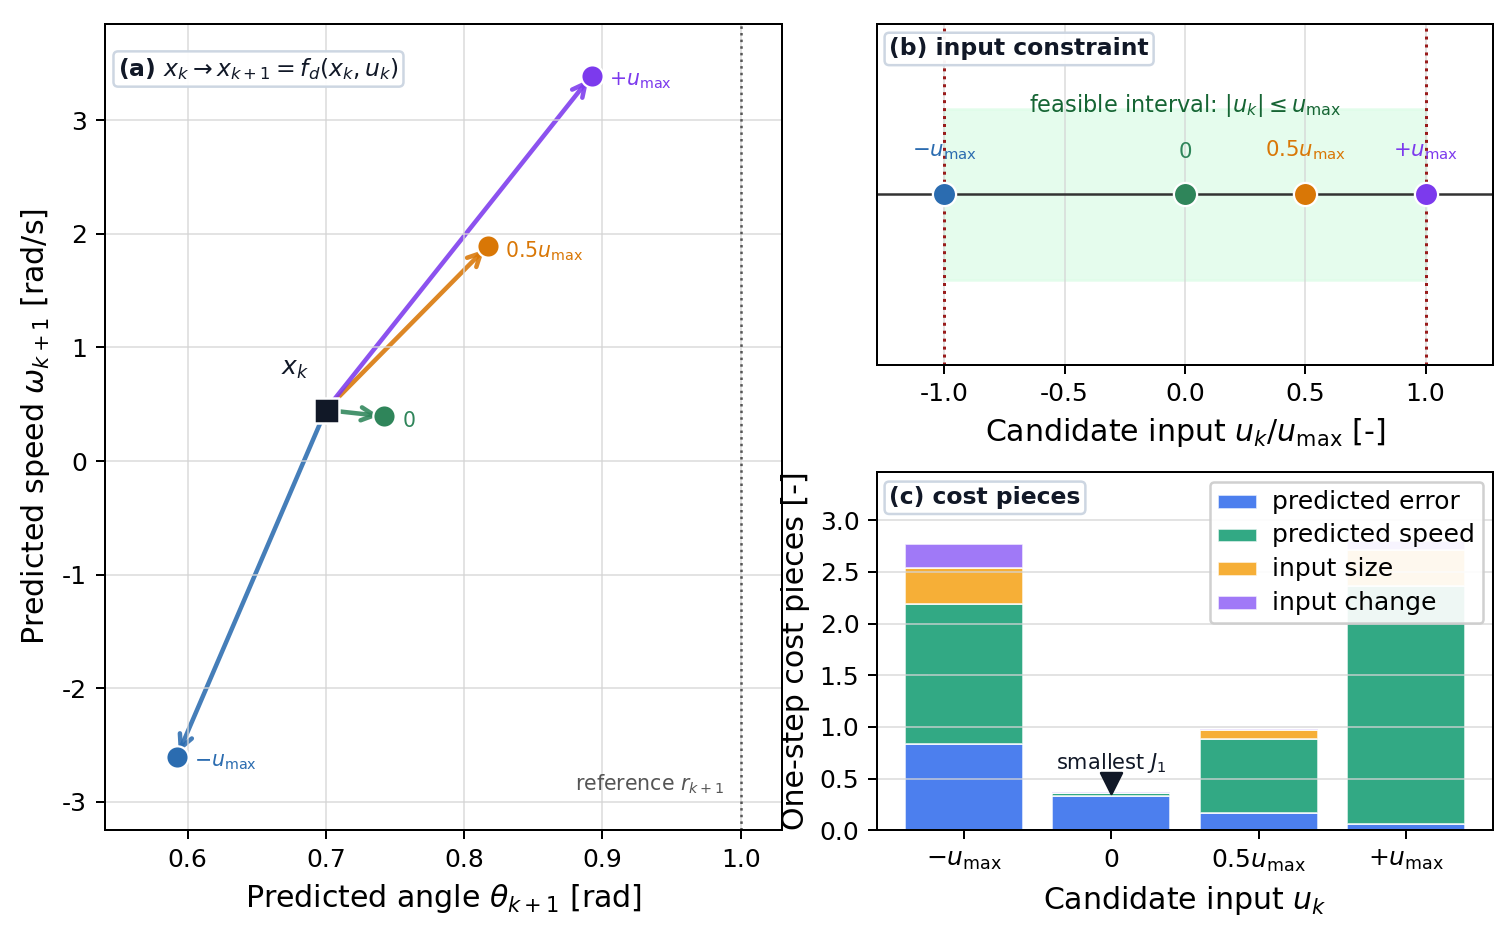
\includegraphics[width=0.98\linewidth,bb=0 0 1512 936]{figures/one_step_horizon_bridge.png}
\caption{性能指標と Pareto 図から作ったスカラー評価を、一段先の入力選択として読むための橋渡し図。現在状態 $x_k$、候補入力 $u_k$、予測された次状態 $x_{k+1}$、入力制約 $|u_k|\leq u_{\max}$、および偏差・速度・入力・入力変化の評価成分を同時に示している。この図は性能指標と Pareto 採点から有限ホライズンの見方へ移る一段の可視化であり、LQR や MPC の導出ではない。}
\label{fig:one-step-horizon-bridge}
\end{figure}

ここでは、未来を一段だけ予測し、次の偏差、次の速度、入力の大きさ、入力変化を同じスカラー評価に入れている。性能指標と Pareto 図で見た「偏差を減らすほど入力が増える」という関係が、この一段先の最適入力選択では評価関数の中へ移る。ただし、この段落の目的は LQR や MPC へ進むことではなく、候補全体を後から採点していた見方を、いま選ぶ入力 $u_k$ の採点へ一段だけ近づけることである。まずこの一段先の形で、重みと制約が入力選択をどう変えるかを読む準備が整う。


\section{状態変数}

伝達関数は入力から出力への関係をよく表すが、内部の量を直接扱いたいときには状態空間表現が必要になる。状態 $x\in\R^n$、入力 $u\in\R^m$、出力 $y\in\R^p$ に対して、線形時不変系は
\begin{align}
  \dot{x}(t)&=Ax(t)+Bu(t),\\
  y(t)&=Cx(t)+Du(t)
  \label{eq:ss}
\end{align}
と書く。$A$ は内部の自然な変化、$B$ は入力の入り方、$C$ は出力として見る向き、$D$ は入力が直接出力へ抜ける成分である。

ベクトルは複数の量を一つの点として扱う記法であり、内積
\begin{equation}
  x^\T y=\sum_{i=1}^{n}x_i y_i
\end{equation}
は向きのそろい具合を表す。ノルム
\begin{equation}
  \norm{x}=\sqrt{x^\T x}
\end{equation}
は状態の大きさを測る。3次元の力学では外積
\begin{equation}
  a\times b=\begin{bmatrix}
    a_2b_3-a_3b_2\\ a_3b_1-a_1b_3\\ a_1b_2-a_2b_1
  \end{bmatrix}
\end{equation}
がモーメントや角運動量に現れる。

行列は線形写像である。ランク $\rank A$ は、行列がどれだけ独立な方向を作れるかを表す。正方行列 $A$ の固有値と固有ベクトルは
\begin{equation}
  Av=\lambda v
\end{equation}
で定義される。状態方程式では、$A$ の固有値が内部モードの速さと振動を決める。

\section{行列指数関数}

入力なしの状態方程式 $\dot{x}=Ax$ の解は
\begin{equation}
  x(t)=e^{At}x(0)
\end{equation}
である。行列指数関数は級数
\begin{equation}
  e^{At}=I+At+\frac{1}{2!}A^2t^2+\frac{1}{3!}A^3t^3+\cdots
\end{equation}
で定義される。$A$ が対角化できて $A=V\Lambda V^{-1}$ なら
\begin{equation}
  e^{At}=V e^{\Lambda t}V^{-1},\qquad
  e^{\Lambda t}=\diag(e^{\lambda_1t},\ldots,e^{\lambda_nt}).
\end{equation}
固有値の実部が負なら対応する指数は減衰し、正なら増大する。

入力がある場合、解は
\begin{equation}
  x(t)=e^{At}x(0)+\int_0^t e^{A(t-\tau)}Bu(\tau)\,\dd\tau
  \label{eq:ss-solution}
\end{equation}
である。第一項は零入力応答、第二項は零状態応答である。状態空間で「自然に動く部分」と「入力で作る部分」を分けて見られるのは、この式があるからである。

\section{離散化}

計算機で制御するには、連続時間モデルをサンプリング周期 $T_s$ の離散時間モデルへ移す。入力をサンプル間で一定とみなすゼロ次ホールドでは
\begin{align}
  x_{k+1}&=A_d x_k+B_d u_k,\\
  A_d&=e^{AT_s},\\
  B_d&=\int_0^{T_s}e^{A\tau}B\,\dd\tau
\end{align}
となる。$A$ が正則なら
\begin{equation}
  B_d=A^{-1}(A_d-I)B
\end{equation}
と計算できる。

もっと粗い近似として、前進オイラー法は
\begin{equation}
  x_{k+1}=x_k+T_s f(x_k,u_k)
\end{equation}
である。4次の Runge--Kutta 法では
\begin{align}
  k_1&=f(x_k,u_k),\\
  k_2&=f(x_k+T_s k_1/2,u_k),\\
  k_3&=f(x_k+T_s k_2/2,u_k),\\
  k_4&=f(x_k+T_s k_3,u_k),\\
  x_{k+1}&=x_k+\frac{T_s}{6}(k_1+2k_2+2k_3+k_4)
\end{align}
と進める。制御計算では、この数値積分の精度と計算時間の釣り合いが重要になる。

\section{可制御性}

状態を望む方向へ動かせるかは、可制御性で決まる。連続時間線形系 \weq{ss} の可制御行列は
\begin{equation}
  \mathcal{C}=\begin{bmatrix}B&AB&A^2B&\cdots&A^{n-1}B\end{bmatrix}
\end{equation}
である。$\rank\mathcal{C}=n$ なら、任意の初期状態から任意の終端状態へ有限時間で移せる。

この式は、入力 $B$ が直接押せる方向だけでなく、$A$ による自然な回転や結合を通じて広がる方向も数えている。倒立振子では、台車の力が直接角度を押すわけではないが、力が台車加速度を作り、拘束を通じて角度へ効くため、可制御になる。

可制御でないモードが不安定なら、どんな状態フィードバックでも安定化できない。制御器の工夫より前に、アクチュエータ配置やモデルの取り方を見直す必要がある。

\section{可観測性}

状態を測れるか、または出力から推定できるかは可観測性で決まる。可観測行列は
\begin{equation}
  \mathcal{O}=\begin{bmatrix}C\\ CA\\ CA^2\\ \vdots\\ CA^{n-1}\end{bmatrix}
\end{equation}
であり、$\rank\mathcal{O}=n$ なら初期状態を出力履歴から一意に復元できる。

可制御性と可観測性は双対である。$(A,B)$ の可制御性は $(A^\T,C^\T)$ の可観測性と同じ形で判定できる。これは、入力で状態へ影響を広げる問題と、状態の影響が出力へ現れる問題が、行列の向きを反転した同じ構造を持つことを意味する。

\section{状態フィードバックと極配置}

状態が利用できるなら、入力を
\begin{equation}
  u=-Kx+r_u
\end{equation}
と作れる。閉ループは
\begin{equation}
  \dot{x}=(A-BK)x+Br_u
\end{equation}
であり、$K$ によって $A-BK$ の固有値を動かす。可制御なら、望む極集合を原理的には配置できる。

SISO 系では、可制御正準形に変換すると極配置の意味が分かりやすい。特性多項式を
\begin{equation}
  \det(sI-A+BK)=s^n+\alpha_{n-1}s^{n-1}+\cdots+\alpha_0
\end{equation}
にしたいなら、$K$ を係数が一致するように選ぶ。実務では極を左へ動かすほど応答は速くなるが、入力が大きくなり、ノイズや未モデル dynamics に弱くなる。

\section{オブザーバと分離定理}

すべての状態が測れるとは限らない。そこで推定状態 $\hat{x}$ を
\begin{equation}
  \dot{\hat{x}}=A\hat{x}+Bu+L(y-C\hat{x})
\end{equation}
で更新する。推定誤差 $e_x=x-\hat{x}$ は
\begin{equation}
  \dot{e}_x=(A-LC)e_x
\end{equation}
に従う。$(A,C)$ が可観測なら、$L$ によって $A-LC$ の極を望ましく置ける。

推定状態を使って $u=-K\hat{x}$ としても、状態フィードバックの極とオブザーバの極は別々に設計できる。これを分離定理という。閉ループ全体の固有値は、$A-BK$ の固有値と $A-LC$ の固有値を合わせたものになる。ただし、分離定理は線形モデルと理想化された条件の話であり、飽和やノイズが強い実装では相互作用を確認する必要がある。

\section{線形系のリアプノフ安定性}

固有値を見る方法は線形系に強いが、同じ安定性をエネルギーのような関数でも表せる。ここではまず線形系だけを見る。平衡点 $x=0$ に対し、正定値関数 $V(x)$ があり
\begin{equation}
  V(x)>0\quad(x\ne0),\qquad V(0)=0
\end{equation}
を満たすとする。さらに軌道に沿った微分
\begin{equation}
  \dot{V}(x)=\frac{\pp V}{\pp x}f(x)
\end{equation}
が負定値なら、平衡点は漸近安定である。

線形系 $\dot{x}=Ax$ では、二次形式
\begin{equation}
  V(x)=x^\T P x,\qquad P=P^\T>0
\end{equation}
を考える。微分は
\begin{equation}
  \dot{V}=x^\T(A^\T P+PA)x
\end{equation}
である。任意の正定値 $Q$ に対して
\begin{equation}
  A^\T P+PA=-Q
\end{equation}
を満たす $P>0$ が存在すれば、$A$ は安定である。このリアプノフ方程式は、次に扱う LQR の価値関数へそのままつながる。

正定値行列は、ベクトルの重み付き大きさを作る行列である。$P>0$ なら $x^\T P x$ は $x\ne0$ で常に正になる。半正定値 $P\ge0$ では 0 になる方向が残る。評価関数や共分散行列で正定値性が重要になるのは、距離や不確かさを破綻なく測るためである。

\section{状態空間の式変形を省略しない}

\begin{theorem}[行列指数関数による解公式]
線形時不変系 $\dot{x}=Ax+Bu$ の解は
\begin{equation}
  x(t)=e^{At}x(0)+\int_0^t e^{A(t-\tau)}Bu(\tau)\,\dd\tau
\end{equation}
である。
\end{theorem}

\begin{derivation}
まず $u=0$ のとき、$x(t)=e^{At}x(0)$ とおく。行列指数関数の微分公式
\begin{equation}
  \frac{\dd}{\dd t}e^{At}=Ae^{At}
\end{equation}
より
\begin{equation}
  \dot{x}(t)=Ae^{At}x(0)=Ax(t)
\end{equation}
である。次に入力がある場合、定数変化法として $x(t)=e^{At}z(t)$ とおく。微分すると
\begin{align}
  \dot{x}(t)&=Ae^{At}z(t)+e^{At}\dot{z}(t),\\
  Ax(t)+Bu(t)&=Ae^{At}z(t)+Bu(t).
\end{align}
両者を等しいとおくと
\begin{equation}
  e^{At}\dot{z}(t)=Bu(t)
\end{equation}
である。左から $e^{-At}$ を掛けて
\begin{equation}
  \dot{z}(t)=e^{-At}Bu(t)
\end{equation}
となる。時刻 $0$ から $t$ まで積分すると
\begin{equation}
  z(t)=z(0)+\int_0^t e^{-A\tau}Bu(\tau)\,\dd\tau.
\end{equation}
$x(0)=z(0)$ なので
\begin{align}
  x(t)&=e^{At}x(0)+e^{At}\int_0^t e^{-A\tau}Bu(\tau)\,\dd\tau\\
  &=e^{At}x(0)+\int_0^t e^{A(t-\tau)}Bu(\tau)\,\dd\tau.
\end{align}
\end{derivation}

\begin{theorem}[Kalman の可制御性ランク条件]
連続時間線形系 $(A,B)$ が可制御であるための必要十分条件は
\begin{equation}
  \rank\begin{bmatrix}B&AB&\cdots&A^{n-1}B\end{bmatrix}=n
\end{equation}
である。
\end{theorem}

\begin{why}
この行列は、入力が直接作る方向 $B$、一度自然な運動 $A$ を通って現れる方向 $AB$、さらに繰り返した方向 $A^2B$ を並べている。ランクが $n$ なら、状態空間のすべての方向を入力から組み合わせて作れる。
\end{why}

\begin{derivation}
オブザーバ誤差の式も省略せずに出す。$y=Cx$、推定器
\begin{equation}
  \dot{\hat{x}}=A\hat{x}+Bu+L(y-C\hat{x})
\end{equation}
を使う。誤差を $e_x=x-\hat{x}$ とおくと
\begin{align}
  \dot{e}_x
  &=\dot{x}-\dot{\hat{x}}\\
  &=(Ax+Bu)-\{A\hat{x}+Bu+L(Cx-C\hat{x})\}\\
  &=A(x-\hat{x})-LC(x-\hat{x})\\
  &=(A-LC)e_x.
\end{align}
したがって $A-LC$ の固有値を左半平面に置けば、推定誤差は減衰する。
\end{derivation}

\begin{theorem}[Lyapunov の直接法]
平衡点 $x=0$ の近くで、正定値関数 $V(x)$ が存在し、軌道に沿った微分 $\dot{V}(x)$ が負定値なら、その平衡点は漸近安定である。
\end{theorem}

線形系で $V=x^\T Px$ と置くとき、$P=P^\T>0$ なら $V$ は正定値である。微分は積の微分公式より
\begin{align}
  \dot{V}
  &=\dot{x}^\T Px+x^\T P\dot{x}\\
  &=(Ax)^\T Px+x^\T P(Ax)\\
  &=x^\T A^\T Px+x^\T PAx\\
  &=x^\T(A^\T P+PA)x.
\end{align}
ここで $A^\T P+PA=-Q$、$Q>0$ なら
\begin{equation}
  \dot{V}=-x^\T Qx<0\quad(x\ne0)
\end{equation}
なので、Lyapunov の直接法より原点は漸近安定である。
\section{最適制御と確率的推定}

小さな台車を目標位置で静止させる制御を考える。位置偏差をすばやく 0 に近づけたいが、モータ電流や推力を大きくしすぎると発熱、飽和、消費電力の問題が生じる。また、位置センサには分解能とノイズがあり、速度を直接測れない場合には、測定値を単純に差分するとノイズが入力へ入りやすい。したがって設計者が同時に扱うべき量は、目標からのずれ、アクチュエータの使用量、測定の信頼度、モデル予測の信頼度である。

本節では、この二つの妥協を線形モデルの上で定式化する。まず、状態が利用でき、入力に明示的な飽和や上下限制約がない場合に、状態偏差と入力偏差の重み付き和を最小にする LQR を導く。次に、状態の一部しか測れず、測定値とモデルに不確かさがある場合に、予測と測定を共分散で重み付けして状態を推定する Kalman フィルタを導く。いずれも、平衡点または目標軌道の近傍で線形化したモデルを用いる基準設計であり、重み行列や共分散行列は、メートル、メートル毎秒、ニュートン、ボルトなどの異なる物理単位を共通の評価量へ換算する役割を持つ。

\subsection{線形最適制御}

状態フィードバックでは、極をどこに置くかを設計者が選んだ。しかし、台車を「速く止める」だけなら極を左へ動かせばよいとしても、同時に「入力をどれだけ節約するか」は極の位置だけでは直接指定しにくい。ここでは状態偏差を $x(t)\in\R^n$、入力偏差を $u(t)\in\R^m$ とし、たとえば $x$ の成分には位置偏差や速度偏差、$u$ にはモータ電流や推力の偏差が入ると考える。対象は動作点まわりで線形化され、行列 $A$ と $B$ は時不変、初期状態は既知、入力飽和はこの段階では扱わないと仮定する。この条件で、線形系
\begin{equation}
  \dot{x}=Ax+Bu
\end{equation}
に対する評価関数
\begin{equation}
  J=\int_0^\infty \{x(t)^\T Qx(t)+u(t)^\T Ru(t)\}\,\dd t
\end{equation}
を置く。$Q=Q^\T\ge0$ は状態のずれへの重み、$R=R^\T>0$ は入力への重みである。積分の中の $x^\T Qx$ と $u^\T Ru$ は同じ評価率の単位を持つように選ぶ。したがって、位置をメートル、速度をメートル毎秒、入力をニュートンで表すなら、$Q$ と $R$ の各成分はそれぞれの二乗単位を評価率へ換算する係数である。$Q$ を大きくすればずれを強く嫌い、$R$ を大きくすれば入力を節約する。

入力を $u=-Kx$ と置くと、閉ループは $\dot{x}=(A-BK)x$ になる。LQR は、すべての安定化ゲインの中から $J$ を最小にする $K$ を選ぶ。最適ゲインは
\begin{equation}
  K=R^{-1}B^\T P
\end{equation}
であり、$P$ は代数リカッチ方程式
\begin{equation}
  A^\T P+PA-PBR^{-1}B^\T P+Q=0
  \label{eq:care}
\end{equation}
を満たす半正定値の安定化解である。$Q>0$ のように状態全体が十分に罰せられる場合には $P>0$ になる。最適コストは
\begin{equation}
  V(x)=x^\T P x
\end{equation}
となる。前節のリアプノフ関数が安定性を評価する関数だったのに対し、ここでの $V$ は「これから必要になる最小コスト」を表す関数でもある。

有限時間を対象にする場合は、終端時刻 $T$ までの評価
\begin{equation}
  J=x(T)^\T S x(T)+\int_0^T(x^\T Qx+u^\T Ru)\,\dd t
\end{equation}
を最小にする。ここで $S\ge0$ は終端時刻で残った状態偏差をどの程度重く評価するかを表す終端重みである。リカッチ方程式は終端条件 $P(T)=S$ から時間を逆向きに解く微分方程式になる。この有限ホライズンの考え方は後で MPC へ進むための前提だが、ここではまだ制約のない連続時間最適制御として理解しておく。

\subsection{変分法と最適性条件}

最適制御では、時刻ごとの入力値を一つずつ選ぶのではなく、区間全体の入力関数 $u(\cdot)$ を選ぶ。したがって評価関数は、数 $u$ の関数ではなく、関数 $u(\cdot)$ を受け取って数を返す汎関数である。典型的な有限時間問題は
\begin{align}
  J[u]
  &=
  \phi(x(T))
  +\int_0^T \ell(x(t),u(t),t)\,\dd t,\\
  \dot{x}(t)&=f(x(t),u(t),t),
  \qquad x(0)=x_0
  \label{eq:oc-general-problem}
\end{align}
で表される。$\ell$ は途中で支払うランニングコスト、$\phi$ は終端コストである。状態 $x(t)\in\R^n$ と入力 $u(t)\in\R^m$ は時刻に依存する関数であり、制御入力を少し変えると、状態軌道全体も変わる。この「関数を少し変えたときの評価関数の一次の変化」を調べる操作を変分という。

許される小さな入力変化を $\eta(t)$ とし、
\begin{equation}
  u_\varepsilon(t)=u(t)+\varepsilon \eta(t)
\end{equation}
と置く。対応する状態を $x_\varepsilon(t)$ と書くと、第一変分は
\begin{equation}
  \delta J
  =
  \left.\frac{\dd}{\dd\varepsilon}J[u_\varepsilon]\right|_{\varepsilon=0}
  \label{eq:first-variation}
\end{equation}
で定義される。通常の一変数関数で最小値の候補が $F'(z)=0$ を満たすように、制約のない十分滑らかな最適入力では、すべての許される $\eta$ に対して $\delta J=0$ が必要条件になる。この条件は必要条件であって、凸性や正定性がなければ大域最小性までは保証しない。

変分の基本形は、入力制御を含まない曲線最適化で確認できる。軌道 $x(t)$ そのものを選び、
\begin{equation}
  J[x]=\int_0^T L(x(t),\dot{x}(t),t)\,\dd t
\end{equation}
を最小にする問題を考える。端点 $x(0)$、$x(T)$ を固定し、$x_\varepsilon=x+\varepsilon \xi$、$\xi(0)=\xi(T)=0$ と置くと
\begin{align}
  \delta J
  &=
  \int_0^T
  \left(
    \frac{\partial L}{\partial x}\xi
    +\frac{\partial L}{\partial \dot{x}}\dot{\xi}
  \right)\,\dd t\\
  &=
  \int_0^T
  \left(
    \frac{\partial L}{\partial x}
    -\frac{\dd}{\dd t}\frac{\partial L}{\partial \dot{x}}
  \right)\xi\,\dd t
  +
  \left[
    \frac{\partial L}{\partial \dot{x}}\xi
  \right]_0^T.
\end{align}
端点固定により境界項は 0 である。任意の $\xi$ に対して $\delta J=0$ となるには、括弧内が各時刻で 0 でなければならない。よって Euler--Lagrange 方程式
\begin{equation}
  \frac{\partial L}{\partial x}
  -\frac{\dd}{\dd t}
  \frac{\partial L}{\partial \dot{x}}
  =0
  \label{eq:euler-lagrange-entry}
\end{equation}
を得る。これは「最適な曲線では、許される微小な曲線変化に対して評価関数の一次変化が消える」という条件である。力学で Euler--Lagrange 方程式が現れるのも同じ変分の構造による。

制御問題では、軌道 $x$ は自由に選べず、状態方程式 $\dot{x}=f(x,u,t)$ に従う。この動的制約を扱うため、随伴変数 $\lambda(t)\in\R^n$ を導入し、拡張された汎関数
\begin{equation}
  \bar{J}
  =
  \phi(x(T))
  +\int_0^T
  \left\{
    \ell(x,u,t)
    +\lambda^\T\bigl(f(x,u,t)-\dot{x}\bigr)
  \right\}\,\dd t
\end{equation}
を考える。最適軌道では $f-\dot{x}=0$ なので、$\bar{J}$ と $J$ の値は一致する。$x$ と $u$ の変分を取り、$\lambda^\T\dot{x}$ の項を部分積分して一次の項を集めると、Pontryagin の Hamiltonian
\begin{equation}
  \mathcal{H}(x,u,\lambda,t)
  =
  \ell(x,u,t)+\lambda^\T f(x,u,t)
  \label{eq:pontryagin-hamiltonian}
\end{equation}
により、内部点の必要条件は
\begin{align}
  \dot{x}&=\frac{\partial \mathcal{H}}{\partial \lambda}
  =f(x,u,t),
  \label{eq:pmp-state}\\
  -\dot{\lambda}&=\frac{\partial \mathcal{H}}{\partial x},
  \label{eq:pmp-costate}\\
  0&=\frac{\partial \mathcal{H}}{\partial u},
  \label{eq:pmp-stationarity}\\
  \lambda(T)&=\frac{\partial \phi}{\partial x}(x(T)).
  \label{eq:pmp-terminal}
\end{align}
となる。$\lambda$ は状態を少し変えたときに将来の最小コストがどれだけ変わるかを表す感度であり、随伴変数または共状態と呼ばれる。状態方程式は初期条件 $x(0)=x_0$ から前向きに進み、随伴方程式は終端条件 \weq{pmp-terminal} から後ろ向きに決まる。したがって、最適制御問題は一般に二点境界値問題になる。入力制約がない滑らかな場合は \weq{pmp-stationarity} を使うが、入力に上下限や不等式制約がある場合は、Hamiltonian を許容集合上で最小にする条件や KKT 条件へ置き換わる。

同じ問題の別表現が動的計画法である。時刻 $t$、状態 $x$ から終端までに達成できる最小残りコストを値関数
\begin{equation}
  V(t,x)=
  \min_{u(\cdot)}
  \left\{
    \phi(x(T))
    +\int_t^T \ell(x(\tau),u(\tau),\tau)\,\dd \tau
  \right\}
  \label{eq:value-function-entry}
\end{equation}
と定義する。短い時間幅 $h>0$ だけ先へ進めると、最適性の原理より
\begin{equation}
  V(t,x)=
  \min_{u(\cdot)}
  \left\{
    \int_t^{t+h}\ell(x(\tau),u(\tau),\tau)\,\dd \tau
    +V(t+h,x(t+h))
  \right\}
  \label{eq:dynamic-programming-principle}
\end{equation}
が成り立つ。右辺は、最初の短い区間で支払うコストと、その後の最小残りコストの和である。$h$ を十分小さくし、$x(t+h)=x+h f(x,u,t)+o(h)$ を代入して Taylor 展開すると
\begin{align}
  0=
  \min_u
  \left\{
    \ell(x,u,t)
    +\frac{\partial V}{\partial t}(t,x)
    +\frac{\partial V}{\partial x}(t,x)^\T f(x,u,t)
  \right\}
  \label{eq:hjb-entry}
\end{align}
を得る。これが Hamilton--Jacobi--Bellman 方程式であり、終端条件は $V(T,x)=\phi(x)$ である。Pontryagin の条件が一つの最適軌道に沿った必要条件を与えるのに対し、HJB 方程式は全状態に対する値関数を求める方程式である。滑らかな値関数が得られる場合、両者は
\begin{equation}
  \lambda(t)=
  \frac{\partial V}{\partial x}(t,x(t))
  \label{eq:costate-value-gradient}
\end{equation}
で結びつく。

LQR では、この一般形が閉じた行列方程式に落ちる。線形系 $f=Ax+Bu$、二次コスト
\begin{equation}
  \ell=x^\T Qx+u^\T Ru,
  \qquad
  \phi=x^\T Sx
\end{equation}
を用いると、Hamiltonian は
\begin{equation}
  \mathcal{H}
  =
  x^\T Qx+u^\T Ru+\lambda^\T(Ax+Bu)
\end{equation}
であり、停留条件から
\begin{equation}
  0=2Ru+B^\T\lambda,
  \qquad
  u=-\frac{1}{2}R^{-1}B^\T\lambda
\end{equation}
を得る。一方、HJB で値関数を $V(t,x)=x^\T P(t)x$ と置けば
\begin{equation}
  \lambda=\partial_x V=2P(t)x
\end{equation}
なので、最適入力は
\begin{equation}
  u=-R^{-1}B^\T P(t)x
\end{equation}
となる。さらに HJB 方程式の二次形式の係数を 0 と置くことでリカッチ微分方程式が得られ、無限ホライズンではその定常解が代数リカッチ方程式になる。したがって、変分、Pontryagin の条件、動的計画法、HJB は別々の公式ではなく、LQR のリカッチ方程式へ至る同じ最適性の構造を異なる表現で見ている。

最後に、一次元の積分器でこの接続を確認する。対象を
\begin{equation}
  \dot{x}=u,
  \qquad x(0)=x_0
\end{equation}
とし、評価関数を
\begin{equation}
  J=sx(T)^2+\int_0^T r u(t)^2\,\dd t,
  \qquad s\ge0,\quad r>0
  \label{eq:scalar-integrator-cost}
\end{equation}
とする。Hamiltonian は
\begin{equation}
  \mathcal{H}=r u^2+\lambda u
\end{equation}
である。最適性条件は
\begin{align}
  \dot{x}&=u,\\
  -\dot{\lambda}&=0,\\
  0&=2ru+\lambda,\\
  \lambda(T)&=2s x(T)
\end{align}
である。したがって $\lambda$ は定数で、$u=-\lambda/(2r)$ も定数になる。終端条件に $x(T)=x_0+Tu$ を代入すると
\begin{align}
  \lambda
  &=2s\left(x_0-\frac{T}{2r}\lambda\right),\\
  \lambda\left(1+\frac{sT}{r}\right)&=2s x_0,\\
  u^*&=-\frac{s}{r+sT}x_0
\end{align}
を得る。同じ結果を HJB から導く。$V(t,x)=P(t)x^2$ と置いたとき
\begin{equation}
  0=\min_u\{r u^2+\dot{P}x^2+2P xu\}
\end{equation}
であり、$u^*=-(P/r)x$、さらに
\begin{equation}
  \dot{P}=\frac{P^2}{r},
  \qquad
  P(T)=s
\end{equation}
となる。このスカラーのリカッチ方程式を解くと
\begin{equation}
  P(t)=\frac{sr}{r+s(T-t)}
  \label{eq:scalar-riccati-solution}
\end{equation}
である。したがって $t=0$ では
\begin{equation}
  u^*(0)=-\frac{P(0)}{r}x_0
  =-\frac{s}{r+sT}x_0
\end{equation}
となり、Pontryagin の条件から得た入力と一致する。この小さな例では、随伴変数、値関数の勾配、リカッチ方程式が同じ最適性条件の別表現であることが直接確認できる。

\subsection{確率とノイズ}

ここまでの制御では、状態 $x$ が分かっているか、少なくともオブザーバで滑らかに推定できると考えた。台車の例では、位置センサから位置は読めても、速度は測れないことが多い。さらに、センサの分解能や電気的な揺らぎにより、測定値をそのまま真値とみなすと入力が細かく振れる。測定値 $y$ を
\begin{equation}
  y=Cx+v
\end{equation}
と書くと、$v$ は測定ノイズである。$y$ の単位は測定量の単位であり、位置センサならメートル、角度センサならラジアンである。平均が 0、分散が $\sigma^2$ のノイズなら
\begin{equation}
  E[v]=0,
  \qquad
  E[v^2]=\sigma^2
\end{equation}
である。多次元では共分散行列
\begin{equation}
  R=E[vv^\T]
\end{equation}
がノイズの大きさと相関を表す。$R$ の $(i,j)$ 成分は、測定 $y_i$ と $y_j$ の単位の積を持つ。

モデルにも不確かさがある。摩擦、坂道、外乱、離散化誤差をすべて正確には書けないため、離散時間モデルを
\begin{align}
  x_{k+1}&=A x_k+B u_k+w_k,\\
  y_k&=C x_k+v_k
\end{align}
と書き、$w_k$ の共分散を $Q$、$v_k$ の共分散を $R$ とする。この導入では記号を簡潔に $Q,R$ と書くが、後の詳細な導出では LQR の重みと区別するためにプロセスノイズ共分散を $Q_w$、測定ノイズ共分散を $R_v$ と書く。$Q$ の成分は状態成分の単位の積、$R$ の成分は測定成分の単位の積を持つ。$Q$ が大きいほどモデルを疑い、$R$ が大きいほどセンサを疑う。推定とは、この二つの信頼度を使って状態を更新することである。

\subsection{カルマンフィルタ}

まず1次元で、予測値と測定値の混ぜ方を確認する。事前推定値を $\hat{x}^-$、その分散を $P^-$、測定値を $y$、測定ノイズ分散を $R$ とする。$x$ が位置なら $P^-$ と $R$ は平方メートルの単位を持ち、値が大きいほどその情報を信じにくいことを表す。更新後の推定値を
\begin{equation}
  \hat{x}=\hat{x}^-+K(y-\hat{x}^-)
\end{equation}
と置くと、$K$ は測定をどれだけ信じるかを表す。誤差分散を最小にするゲインは
\begin{equation}
  K=\frac{P^-}{P^-+R}
\end{equation}
である。事前分散が大きいほど測定を信じ、測定ノイズが大きいほど事前値を信じる。

多次元のカルマンフィルタは、線形モデルに対する予測と更新で書ける。
\begin{align}
  \hat{x}_{k|k-1}&=A\hat{x}_{k-1|k-1}+Bu_{k-1},\\
  P_{k|k-1}&=AP_{k-1|k-1}A^\T+Q,\\
  K_k&=P_{k|k-1}C^\T(CP_{k|k-1}C^\T+R)^{-1},\\
  \hat{x}_{k|k}&=\hat{x}_{k|k-1}+K_k(y_k-C\hat{x}_{k|k-1}),\\
  P_{k|k}&=(I-K_kC)P_{k|k-1}.
\end{align}
ここで $P$ は推定誤差の共分散である。カルマンフィルタは、線形ガウス系では平均二乗誤差を最小にする推定器である。

LQR は状態が利用可能である場合の最適状態フィードバックであり、Kalman フィルタは線形確率モデルにおける状態推定器である。線形ガウス仮定のもとでは、Kalman フィルタで得た $\hat{x}$ を LQR の状態フィードバックへ入力する構成が LQG 制御を与える。本節では、対象および推定器を線形として扱う。

\subsection{LQR を平方完成で導く}

極配置では、閉ループ極を指定して応答の速さや減衰を設計した。しかし、台車の位置をすばやく戻したい一方で加える力には上限がある、あるいはモータの角度誤差を小さくしたい一方で電流を大きくしすぎたくない、という設計では、極だけでは「状態のずれ」と「入力の大きさ」をどの割合で許すかを数値で比較できない。極を速く置けば偏差は早く消えるが、一般に入力は大きくなり、飽和や発熱の制約に近づく。そこで、状態偏差を二次形式 $x^\T Qx$、入力努力を $u^\T Ru$ として同じ評価関数へ入れ、重み $Q,R$ によってその交換条件を明示する。平方完成は、この二次評価の中で入力 $u$ がどの値を選ぶと残りコストを最も小さくするかを直接取り出すために用いる。

\begin{theorem}[連続時間 LQR のリカッチ方程式]
$(A,B)$ が可安定で、$(A,Q^{1/2})$ が可検出である線形系 $\dot{x}=Ax+Bu$ に対し、評価関数
\begin{equation}
  J=\int_0^\infty (x^\T Qx+u^\T Ru)\,\dd t,
  \qquad Q=Q^\T\ge0,
  \quad R=R^\T>0
\end{equation}
を最小にする状態フィードバックは
\begin{equation}
  u=-R^{-1}B^\T Px
\end{equation}
であり、$P$ は代数リカッチ方程式
\begin{equation}
  A^\T P+PA-PBR^{-1}B^\T P+Q=0
\end{equation}
を満たす半正定値の安定化解である。
\end{theorem}

\begin{derivation}
最適な残りコストが二次形式
\begin{equation}
  V(x)=x^\T Px
\end{equation}
で表せると仮定する。最適制御の動的計画法、すなわち Hamilton--Jacobi--Bellman 方程式より
\begin{equation}
  0=\min_u\{x^\T Qx+u^\T Ru+\dot{V}(x)\}
\end{equation}
である。$\dot{x}=Ax+Bu$ なので
\begin{align}
  \dot{V}
  &=\dot{x}^\T Px+x^\T P\dot{x}\\
  &=(Ax+Bu)^\T Px+x^\T P(Ax+Bu)\\
  &=x^\T A^\T Px+u^\T B^\T Px+x^\T PAx+x^\T PBu.
\end{align}
スカラーは転置しても同じなので $u^\T B^\T Px=x^\T PBu$ である。したがって
\begin{equation}
  \dot{V}=x^\T(A^\T P+PA)x+2u^\T B^\T Px.
\end{equation}
HJB 方程式の中身は
\begin{equation}
  x^\T Qx+x^\T(A^\T P+PA)x+u^\T Ru+2u^\T B^\T Px
\end{equation}
である。$u$ に関する部分を平方完成する。
\begin{align}
  u^\T Ru+2u^\T B^\T Px
  &=(u+R^{-1}B^\T Px)^\T R(u+R^{-1}B^\T Px)\\
  &\quad -x^\T PBR^{-1}B^\T Px.
\end{align}
第一項は $R>0$ より非負であり、最小にするには
\begin{equation}
  u+R^{-1}B^\T Px=0
\end{equation}
とすればよい。よって
\begin{equation}
  u=-R^{-1}B^\T Px
\end{equation}
である。残りの $x$ に関する項が任意の $x$ で 0 になる必要があるので
\begin{equation}
  A^\T P+PA-PBR^{-1}B^\T P+Q=0
\end{equation}
を得る。
\end{derivation}

\subsection{有限ホライズン LQR とリカッチ微分方程式}

無限ホライズン LQR では、残り時間がいつも無限にあるため、最適な残りコスト $V(x)=x^\T Px$ は時刻に依存しなかった。有限ホライズンでは事情が変わる。終端時刻 $T$ が近づけば、入力を使って状態を戻す余裕が少なくなるので、同じ状態 $x$ に対する「残りコスト」は現在時刻 $t$ によって変わる。したがって、値関数は
\begin{equation}
  V(t,x)=\min_{u(\cdot)}
  \left\{
    x(T)^\T S x(T)
    +\int_t^T
      \left(x(\tau)^\T Qx(\tau)+u(\tau)^\T Ru(\tau)\right)\,\dd \tau
  \right\}
  \label{eq:finite-lqr-value}
\end{equation}
と書く。状態は $x(t)\in\R^n$、入力は $u(t)\in\R^m$、システムは
\begin{equation}
  \dot{x}(\tau)=Ax(\tau)+Bu(\tau),
  \qquad x(t)=x
\end{equation}
である。ここでは $A,B,Q,R,S$ は時不変とし、$Q=Q^\T\ge0$、$R=R^\T>0$、$S=S^\T\ge0$ を仮定する。$Q$ は途中の状態偏差を罰する重み、$R$ は途中の入力の大きさを罰する重み、$S$ は終端時刻に残った状態偏差を罰する重みである。単位を持つ物理量を扱うときは、$x^\T Qx$、$u^\T Ru$、$x(T)^\T S x(T)$ が同じ「評価関数の単位」になるように重みを選ぶ。$Q$ を大きくすると途中のずれを嫌い、$R$ を大きくすると入力を節約し、$S$ を大きくすると終端で原点や目標偏差へ近づけることを強く求める。後の MPC の記号では、この終端重みを $P_f$ と書くことが多い。

動的計画法では、時刻 $t$ で少しだけ進んだ後も、残り区間では同じ形の最適化問題を解くと考える。連続時間の Hamilton--Jacobi--Bellman 方程式は
\begin{equation}
  0=\min_u
  \left\{
    x^\T Qx+u^\T Ru
    +\partial_t V(t,x)
    +\partial_x V(t,x)^\T(Ax+Bu)
  \right\}
  \label{eq:finite-lqr-hjb}
\end{equation}
であり、終端条件は
\begin{equation}
  V(T,x)=x^\T S x
  \label{eq:finite-lqr-terminal-value}
\end{equation}
である。線形系と二次評価関数の組では、値関数も二次形式になると予想できるので
\begin{equation}
  V(t,x)=x^\T P(t)x,
  \qquad P(t)=P(t)^\T
  \label{eq:finite-lqr-ansatz}
\end{equation}
と置く。この形を仮定して HJB 方程式へ代入し、最後にその仮定が閉じていることを確かめる。まず
\begin{align}
  \partial_t V(t,x)&=x^\T \dot{P}(t)x,\\
  \partial_x V(t,x)&=2P(t)x
\end{align}
である。したがって
\begin{align}
  \partial_x V^\T(Ax+Bu)
  &=2x^\T P(t)Ax+2x^\T P(t)Bu\\
  &=x^\T\{A^\T P(t)+P(t)A\}x+2u^\T B^\T P(t)x
\end{align}
となる。二つ目の等号では、$x^\T P A x$ がスカラーであり、転置して $x^\T A^\T P x$ と足し合わせられることを使った。

\weq{finite-lqr-hjb} の中で $u$ に依存する部分は
\begin{equation}
  u^\T Ru+2u^\T B^\T P(t)x
\end{equation}
である。これは前の無限ホライズン LQR と同じ平方完成で
\begin{align}
  u^\T Ru+2u^\T B^\T P(t)x
  &=
  \left(u+R^{-1}B^\T P(t)x\right)^\T
  R
  \left(u+R^{-1}B^\T P(t)x\right)\\
  &\quad
  -x^\T P(t)BR^{-1}B^\T P(t)x
\end{align}
と整理できる。$R>0$ なので第一項は非負であり、最小値は
\begin{equation}
  u^*(t)=-R^{-1}B^\T P(t)x(t)
  \label{eq:finite-lqr-control}
\end{equation}
で達成される。したがって有限ホライズン LQR のフィードバックゲインは
\begin{equation}
  K(t)=R^{-1}B^\T P(t)
  \label{eq:finite-lqr-gain}
\end{equation}
であり、一般には時刻によって変わる。

最小化後の HJB 方程式に残る $x$ の二次形式は
\begin{equation}
  x^\T
  \left\{
    \dot{P}
    +A^\T P+PA
    -PBR^{-1}B^\T P
    +Q
  \right\}
  x=0
\end{equation}
である。これは任意の $x$ で成り立たなければならないので、行列の係数が 0 になる。よって有限ホライズン連続時間 LQR のリカッチ微分方程式
\begin{equation}
  -\dot{P}(t)
  =
  A^\T P(t)+P(t)A
  -P(t)BR^{-1}B^\T P(t)
  +Q,
  \qquad P(T)=S
  \label{eq:finite-lqr-rde}
\end{equation}
を得る。右端の $P(T)=S$ は初期条件ではなく終端条件である。したがって、数値計算では $t=T$ から $t=0$ へ向かって逆向きに解くか、残り時間 $\sigma=T-t$ を導入して前向きの微分方程式として解く。$P(t)$ が得られれば、各時刻で \weq{finite-lqr-control} を用いるだけでよい。

同じ式は Hamiltonian の最適性条件からも確認できる。Hamiltonian を
\begin{equation}
  \mathcal{H}(x,u,\lambda)
  =x^\T Qx+u^\T Ru+\lambda^\T(Ax+Bu)
\end{equation}
と置くと、最適性条件は
\begin{align}
  0&=\frac{\partial \mathcal{H}}{\partial u}
    =2Ru+B^\T\lambda,\\
  -\dot{\lambda}&=\frac{\partial \mathcal{H}}{\partial x}
    =2Qx+A^\T\lambda,\\
  \lambda(T)&=2Sx(T)
\end{align}
である。値関数から得られる関係 $\lambda=\partial_x V=2P(t)x$ を代入すると
\begin{equation}
  u^*=-\frac{1}{2}R^{-1}B^\T\lambda
  =-R^{-1}B^\T P(t)x
\end{equation}
となる。さらに
\begin{align}
  \dot{\lambda}
  &=2\dot{P}x+2P\dot{x}\\
  &=2\dot{P}x+2P(Ax-BR^{-1}B^\T Px)
\end{align}
である。これを随伴方程式 $-\dot{\lambda}=2Qx+2A^\T Px$ と比べれば
\begin{equation}
  \dot{P}+A^\T P+PA-PBR^{-1}B^\T P+Q=0
\end{equation}
が再び得られる。動的計画法では「残りコスト」を直接扱い、Hamiltonian 形式では「状態の変化に対するコストの感度」である随伴変数を扱うが、LQR では両者が $\lambda=2Px$ で同じ内容に結びつく。

前の平方完成による無限ホライズン LQR は、有限ホライズンの式から $\dot{P}=0$ となる定常解を取り出したものと見られる。残り時間が十分長く、$(A,B)$ が可安定で $(A,Q^{1/2})$ が可検出なら、$P(t)$ は多くの場合、区間の内側で代数リカッチ方程式の安定化解 $P_\infty$ に近づく。すなわち
\begin{equation}
  A^\T P_\infty+P_\infty A
  -P_\infty BR^{-1}B^\T P_\infty+Q=0
\end{equation}
であり、$K_\infty=R^{-1}B^\T P_\infty$ が時間不変ゲインになる。

有限ホライズンの終端重み $S$ は、後で扱う MPC の終端コストと同じ役割を持つ。MPC では制約を含むため、各サンプル時刻で有限ホライズン問題を解き直し、最初の入力だけを使う。ホライズンの先をまったく考えないと、予測区間の終わりで不自然な入力や状態が選ばれることがある。そのため終端コスト $V_f(x)=x^\T P_f x$ を置き、$P_f$ に LQR のリカッチ解を使う。これは、予測区間の外側で局所 LQR を続けたときの残りコストを有限ホライズン問題の末端へ折り込む操作である。

\subsection{離散時間 LQR と代数リカッチ方程式}

デジタル制御器では、入力はサンプリング時刻ごとに更新される。サンプリング周期を $h>0$ とし、零次ホールドや数値積分により得られた離散時間モデルを
\begin{equation}
  x_{k+1}=A_d x_k+B_d u_k
  \label{eq:dlqr-system}
\end{equation}
と書く。ここで $x_k\in\R^n$ は時刻 $kh$ の状態偏差、$u_k\in\R^m$ は区間 $[kh,(k+1)h)$ で保持される入力偏差であり、$A_d\in\R^{n\times n}$、$B_d\in\R^{n\times m}$ はサンプル周期を含む行列である。以下では、$A_d,B_d$ は時不変、初期状態 $x_0$ は既知、入力には明示的な上下限制約がないと仮定する。重み行列は
\begin{equation}
  Q_x=Q_x^\T\ge0,
  \qquad
  R_u=R_u^\T>0,
  \qquad
  S_N=S_N^\T\ge0
\end{equation}
とし、有限ホライズン評価関数を
\begin{equation}
  J_N
  =
  x_N^\T S_N x_N
  +\sum_{k=0}^{N-1}
  \left(x_k^\T Q_x x_k+u_k^\T R_u u_k\right)
  \label{eq:dlqr-finite-cost}
\end{equation}
で定める。$Q_x$ はサンプル時刻での状態偏差、$R_u$ は入力の大きさ、$S_N$ はホライズン末端の状態偏差を評価する。連続時間評価を離散化して対応させる場合、単純な近似では $Q_x\simeq hQ_c$、$R_u\simeq hR_c$ と置くが、実際には $A_d,B_d$ も $h$ に依存するため、サンプリング周期を変えたときは重みとゲインを同時に再評価する。

動的計画法により、時刻 $k$ から終端までの最小残りコストを
\begin{equation}
  V_k(x)=x^\T P_k x,
  \qquad P_k=P_k^\T
  \label{eq:dlqr-value}
\end{equation}
と置く。終端条件は
\begin{equation}
  P_N=S_N
  \label{eq:dlqr-terminal}
\end{equation}
である。時刻 $k$ では
\begin{align}
  V_k(x)
  =
  \min_u
  \{x^\T Q_x x+u^\T R_u u
  +(A_d x+B_d u)^\T P_{k+1}(A_d x+B_d u)\}
  \label{eq:dlqr-bellman}
\end{align}
が成り立つ。\weq{dlqr-bellman} の中身を展開すると
\begin{align}
  &x^\T(Q_x+A_d^\T P_{k+1}A_d)x\\
  &\quad
  +2u^\T B_d^\T P_{k+1}A_d x
  +u^\T(R_u+B_d^\T P_{k+1}B_d)u
  \label{eq:dlqr-expanded}
\end{align}
となる。$P_{k+1}\ge0$ なら
\begin{equation}
  H_k=R_u+B_d^\T P_{k+1}B_d
  \label{eq:dlqr-hessian}
\end{equation}
は正定値である。したがって、$u$ に関する二次式は平方完成により
\begin{align}
  &u^\T H_k u+2u^\T B_d^\T P_{k+1}A_d x\\
  &=
  (u+H_k^{-1}B_d^\T P_{k+1}A_d x)^\T
  H_k
  (u+H_k^{-1}B_d^\T P_{k+1}A_d x)\\
  &\quad
  -x^\T A_d^\T P_{k+1}B_d
  H_k^{-1}
  B_d^\T P_{k+1}A_d x
  \label{eq:dlqr-completion}
\end{align}
と整理できる。第一項は非負であり、最小値は
\begin{equation}
  u_k^*=-K_kx_k
  \label{eq:dlqr-optimal-input}
\end{equation}
で達成される。ここで有限ホライズンの離散時間 LQR ゲインは
\begin{equation}
  K_k
  =
  (R_u+B_d^\T P_{k+1}B_d)^{-1}
  B_d^\T P_{k+1}A_d
  \label{eq:dlqr-finite-gain}
\end{equation}
である。最小化後の $x$ の二次形式を $x^\T P_kx$ と同一視すると、後退リカッチ再帰
\begin{equation}
  P_k
  =
  Q_x+A_d^\T P_{k+1}A_d
  -A_d^\T P_{k+1}B_d
  (R_u+B_d^\T P_{k+1}B_d)^{-1}
  B_d^\T P_{k+1}A_d,
  \qquad k=N-1,\ldots,0
  \label{eq:dlqr-backward-riccati}
\end{equation}
を得る。これは終端条件 $P_N=S_N$ から時刻を逆向きに計算する差分方程式である。連続時間のリカッチ微分方程式と同様に、終端から現在へ向かって残りコストを伝播させ、その結果として時刻依存ゲイン $K_k$ が定まる。

ホライズンを十分長くし、時不変な重みを使うと、条件が整っている場合には $P_k$ がホライズン内側で一定行列へ近づく。この定常行列を $P_\infty$ と書くと、離散時間代数リカッチ方程式
\begin{equation}
  P_\infty
  =
  Q_x+A_d^\T P_\infty A_d
  -A_d^\T P_\infty B_d
  (R_u+B_d^\T P_\infty B_d)^{-1}
  B_d^\T P_\infty A_d
  \label{eq:dare}
\end{equation}
を満たす。対応する定常ゲインは
\begin{equation}
  K_\infty
  =
  (R_u+B_d^\T P_\infty B_d)^{-1}
  B_d^\T P_\infty A_d
  \label{eq:dlqr-infinite-gain}
\end{equation}
であり、閉ループ行列は
\begin{equation}
  A_d-B_d K_\infty
  \label{eq:dlqr-closed-loop}
\end{equation}
となる。離散時間では、安定性はこの行列の固有値が複素平面の単位円内に入ること、すなわち Schur 安定であることで判定する。

\begin{theorem}[離散時間 LQR の安定化解]
$Q_x=Q_x^\T\ge0$、$R_u=R_u^\T>0$ とする。$(A_d,B_d)$ が可安定で、$(A_d,Q_x^{1/2})$ が可検出であれば、離散時間代数リカッチ方程式 \weq{dare} には半正定値の一意な安定化解 $P_\infty$ が存在する。この解から得られる $K_\infty$ に対して、$A_d-B_d K_\infty$ は Schur 安定になる。
\end{theorem}

この条件の意味は、制御入力で安定化できない不安定モードを残さず、重み $Q_x$ が罰しない不安定モードを見逃さないことである。$Q_x$ が半正定値で一部の状態を直接罰しなくても、その状態が罰せられる状態へ動的に結合していれば可検出性により安定化解は保たれる。一方、入力が作用しない不安定モードや、評価関数にまったく現れない不安定モードがあると、有限の二次コストで全状態を安定化する定常ゲインは一般に得られない。

重みの調整は連続時間 LQR と同じ考え方を持つが、離散時間ではサンプル周期と入力保持の効果が加わる。$Q_x$ を大きくするとサンプル時刻ごとの状態偏差を強く抑えるため、応答は速くなりやすいが、入力振幅やアクチュエータ飽和への余裕は小さくなる。$R_u$ を大きくすると入力を節約し、閉ループ極は一般に開ループ側へ近づく。$S_N$ は有限ホライズン末端で残った状態を評価する重みであり、MPC では \weq{dare} の安定化解を終端コストとして用いると、予測区間の外側で定常 LQR を続ける近似になる。したがって、離散時間 LQR はデジタル実装のための設計法であると同時に、制約を含む MPC の終端設計を支える基準問題でもある。

\subsection{離散時間 Kalman フィルタを予測と更新から導く}

Kalman フィルタは、モデルに基づく予測と測定値に基づく更新から構成される。この二段構造は、線形確率モデルの条件付き平均と誤差共分散の計算により得られる。LQR の重み行列と区別するため、プロセスノイズの共分散を $Q_{w,k}$、測定ノイズの共分散を $R_{v,k}$ と書く。

離散時間の線形モデルを
\begin{align}
  x_k&=A_{k-1}x_{k-1}+B_{k-1}u_{k-1}+G_{k-1}w_{k-1},\label{eq:kf-state-model}\\
  y_k&=C_kx_k+v_k
  \label{eq:kf-measurement-model}
\end{align}
とする。状態は $x_k\in\R^n$、入力は $u_k\in\R^m$、測定は $y_k\in\R^p$ である。$w_k$ はモデル化できなかった外乱や離散化誤差をまとめたプロセスノイズ、$v_k$ はセンサノイズである。仮定は
\begin{align}
  E[w_i]&=0,
  &E[v_i]&=0,\\
  E[w_iw_j^\T]&=Q_{w,i}\delta_{ij},
  &E[v_iv_j^\T]&=R_{v,i}\delta_{ij},\\
  E[w_iv_j^\T]&=0
\end{align}
であり、初期推定誤差 $x_0-\hat{x}_{0|0}$ もすべての $w_i,v_i$ と相関しないとする。ここで $\delta_{ij}$ は $i=j$ で 1、そうでなければ 0 になるクロネッカーのデルタである。さらに予測平均の式では、$w_{k-1}$ が過去の測定履歴 $\mathcal{Y}_{k-1}$ に対してゼロ条件付き平均
\begin{equation}
  E[w_{k-1}\mid\mathcal{Y}_{k-1}]=0
\end{equation}
を持つことを仮定する。独立な白色ノイズを仮定すれば、この条件は満たされる。条件付き平均推定として最適性を述べるときは、これらの確率変数が同時正規分布に従う線形ガウス系を仮定する。ガウス性を仮定しない場合、以下の更新は線形な革新更新に制限した最小平均二乗誤差推定として解釈する。

時刻 $k$ までの測定履歴を
\begin{equation}
  \mathcal{Y}_k=\{y_0,y_1,\ldots,y_k\}
\end{equation}
と書く。推定値 $\hat{x}_{k|k}$ は $\mathcal{Y}_k$ を見た後の状態推定、$\hat{x}_{k|k-1}$ は $\mathcal{Y}_{k-1}$ までを見て時刻 $k$ を予測した値である。対応する推定誤差と共分散を
\begin{align}
  e_{k|k}&=x_k-\hat{x}_{k|k},
  &P_{k|k}&=E[e_{k|k}e_{k|k}^\T\mid\mathcal{Y}_k],\\
  e_{k|k-1}&=x_k-\hat{x}_{k|k-1},
  &P_{k|k-1}&=E[e_{k|k-1}e_{k|k-1}^\T\mid\mathcal{Y}_{k-1}]
\end{align}
と定義する。

まず予測を導く。$u_{k-1}$ は時刻 $k-1$ で与えた既知の入力なので、\weq{kf-state-model} の条件付き期待値を取ると
\begin{align}
  \hat{x}_{k|k-1}
  &=E[x_k\mid\mathcal{Y}_{k-1}]\\
  &=A_{k-1}E[x_{k-1}\mid\mathcal{Y}_{k-1}]+B_{k-1}u_{k-1}
    +G_{k-1}E[w_{k-1}\mid\mathcal{Y}_{k-1}]\\
  &=A_{k-1}\hat{x}_{k-1|k-1}+B_{k-1}u_{k-1}
\end{align}
となる。最後の等号では、$E[w_{k-1}\mid\mathcal{Y}_{k-1}]=0$ を使った。予測誤差は
\begin{align}
  e_{k|k-1}
  &=x_k-\hat{x}_{k|k-1}\\
  &=A_{k-1}(x_{k-1}-\hat{x}_{k-1|k-1})+G_{k-1}w_{k-1}\\
  &=A_{k-1}e_{k-1|k-1}+G_{k-1}w_{k-1}
\end{align}
である。したがって共分散は
\begin{align}
  P_{k|k-1}
  &=E[e_{k|k-1}e_{k|k-1}^\T\mid\mathcal{Y}_{k-1}]\\
  &=A_{k-1}P_{k-1|k-1}A_{k-1}^\T+G_{k-1}Q_{w,k-1}G_{k-1}^\T
\end{align}
になる。途中に出る $E[e_{k-1|k-1}w_{k-1}^\T]$ とその転置は、推定誤差と新しいプロセスノイズが無相関であるため消える。

次に測定値に基づく更新を導く。予測された測定値は
\begin{equation}
  \hat{y}_{k|k-1}=C_k\hat{x}_{k|k-1}
\end{equation}
であり、実際の測定との差
\begin{equation}
  \nu_k=y_k-\hat{y}_{k|k-1}=y_k-C_k\hat{x}_{k|k-1}
\end{equation}
を革新という。\weq{kf-measurement-model} を代入すると
\begin{align}
  \nu_k
  &=C_kx_k+v_k-C_k\hat{x}_{k|k-1}\\
  &=C_ke_{k|k-1}+v_k
\end{align}
なので、その共分散は
\begin{align}
  S_k
  &=E[\nu_k\nu_k^\T\mid\mathcal{Y}_{k-1}]\\
  &=C_kP_{k|k-1}C_k^\T+R_{v,k}
\end{align}
である。$S_k$ は革新共分散と呼ばれ、予測誤差共分散を測定空間へ写した項と測定ノイズ共分散の和である。

更新式を、革新に行列ゲイン $K_k$ を掛けて足す形
\begin{equation}
  \hat{x}_{k|k}=\hat{x}_{k|k-1}+K_k\nu_k
  \label{eq:kf-update-mean}
\end{equation}
に限って考える。以下では、線形な革新更新の範囲で $K_k$ を選ぶ。更新後の誤差は
\begin{align}
  e_{k|k}
  &=x_k-\hat{x}_{k|k}\\
  &=x_k-\hat{x}_{k|k-1}-K_k(C_ke_{k|k-1}+v_k)\\
  &=(I-K_kC_k)e_{k|k-1}-K_kv_k.
\end{align}
したがって、任意の $K_k$ に対する更新後共分散は次式で表される。線形ガウス仮定のもとでは、この共分散は革新の実現値に依存しない。ガウス性を仮定しない場合、次式は $\mathcal{Y}_{k-1}$ で条件付けた線形最小平均二乗誤差の共分散として解釈する。
\begin{equation}
  P_{k|k}(K_k)
  =(I-K_kC_k)P_{k|k-1}(I-K_kC_k)^\T+K_kR_{v,k}K_k^\T
  \label{eq:joseph-form-general}
\end{equation}
である。この式でも、$e_{k|k-1}$ と $v_k$ の交差共分散が 0 であることを使っている。

ゲインは $\tr P_{k|k}(K_k)$ を最小にするように選ぶ。記号を軽くするため、この段落だけ
\begin{equation}
  P^-=P_{k|k-1},
  \qquad C=C_k,
  \qquad R=R_{v,k},
  \qquad S=CP^-C^\T+R
\end{equation}
と書く。\weq{joseph-form-general} を展開すると
\begin{align}
  P(K)
  &=P^- -KCP^- -P^-C^\T K^\T+K(CP^-C^\T+R)K^\T\\
  &=P^- -KCP^- -P^-C^\T K^\T+KSK^\T.
\end{align}
ここで
\begin{equation}
  K_\text{opt}=P^-C^\T S^{-1}
\end{equation}
と置けば、$K_\text{opt}S=P^-C^\T$ が成り立つ。平方完成と同じ形に整理すると
\begin{align}
  P(K)
  &=P^- -K_\text{opt}S K_\text{opt}^\T
    +(K-K_\text{opt})S(K-K_\text{opt})^\T.
\end{align}
$R=R^\T>0$ なら $S>0$ であり、最後の項は半正定値である。したがって $\tr P(K)$ を最小にするのは $K=K_\text{opt}$ で、Kalman ゲインは
\begin{equation}
  K_k=P_{k|k-1}C_k^\T
  (C_kP_{k|k-1}C_k^\T+R_{v,k})^{-1}
  \label{eq:kf-gain-derived}
\end{equation}
となる。

最適ゲインを代入した共分散更新は、簡略形として
\begin{align}
  P_{k|k}
  &=P_{k|k-1}-K_kS_kK_k^\T\\
  &=(I-K_kC_k)P_{k|k-1}
  \label{eq:kf-covariance-simple}
\end{align}
と書ける。二つ目の等号では $K_kS_k=P_{k|k-1}C_k^\T$ を使った。数式上はこれでよいが、有限精度演算では丸め誤差によって $P_{k|k}$ の対称性や半正定値性が崩れることがある。そのため実装では、代数的には同値な Joseph 形式
\begin{equation}
  P_{k|k}
  =(I-K_kC_k)P_{k|k-1}(I-K_kC_k)^\T+K_kR_{v,k}K_k^\T
  \label{eq:kf-joseph-form}
\end{equation}
を用いる。Joseph 形式は左右対称な積で構成されるため、共分散行列の対称性および半正定値性を保ちやすい。

以上をまとめると、離散時間 Kalman フィルタは
\begin{align}
  \hat{x}_{k|k-1}&=A_{k-1}\hat{x}_{k-1|k-1}+B_{k-1}u_{k-1},\\
  P_{k|k-1}&=A_{k-1}P_{k-1|k-1}A_{k-1}^\T
    +G_{k-1}Q_{w,k-1}G_{k-1}^\T,\\
  \nu_k&=y_k-C_k\hat{x}_{k|k-1},\\
  S_k&=C_kP_{k|k-1}C_k^\T+R_{v,k},\\
  K_k&=P_{k|k-1}C_k^\T S_k^{-1},\\
  \hat{x}_{k|k}&=\hat{x}_{k|k-1}+K_k\nu_k,\\
  P_{k|k}&=(I-K_kC_k)P_{k|k-1}(I-K_kC_k)^\T+K_kR_{v,k}K_k^\T
\end{align}
で与えられる。$G_{k-1}=I$ とすれば、$P_{k|k-1}=AP_{k-1|k-1}A^\T+Q$ の形に一致する。

一次元で $C=1$ とすれば、革新共分散は $S=P^-+R$、ゲインは
\begin{equation}
  K=\frac{P^-}{P^-+R}
\end{equation}
である。予測分散 $P^-$ が大きいほど測定値の重みが大きくなり、測定ノイズ分散 $R$ が大きいほど予測値の重みが大きくなる。たとえば熱系の室温推定では、外乱や未モデル化熱流が大きい場合に $Q_w$ を大きく設定し、温度センサの分散が大きい場合に $R_v$ を大きく設定する。

\subsubsection{LQR 重みと Kalman 共分散の可視化}

二次形式の重みは、式だけで扱うと単なる係数として残りやすい。しかし閉ループ応答、入力指令、リカッチ方程式の収束、推定誤差共分散を同じモデルで並べると、重みが設計上のどの妥協に対応するかを確認できる。図\ref{fig:lqr-kalman-examples}では、サンプル周期 $h=0.1\,\mathrm{s}$ の二重積分器
\begin{equation}
  x_{k+1}
  =
  \begin{bmatrix}
    1 & h\\
    0 & 1
  \end{bmatrix}x_k
  +
  \begin{bmatrix}
    h^2/2\\
    h
  \end{bmatrix}u_k,
  \qquad
  y_k=\begin{bmatrix}1&0\end{bmatrix}x_k+v_k
\end{equation}
を用いている。状態は位置偏差と速度偏差であり、測定は位置だけである。上段左は $Q_x=\diag(1,0.08)$ を固定して入力重み $R_u$ を変えたときの位置偏差、上段右は対応する LQR の入力指令 $u_c=-Kx$ である。$R_u$ が小さいほど偏差は早く消えるが、入力指令は大きくなり、図中の点線で示した入力限界を越えやすくなる。ここで描いているのは制御器が要求する指令 $u_c$ であり、実際のアクチュエータに飽和があれば対象へ入る入力は $u_a=\operatorname{sat}(u_c)$ である。したがって実装検証では、推定器とシミュレーションに $u_c$ ではなく実際に印加された $u_a$ を渡す必要がある。

\begin{figure}[tb]
\centering
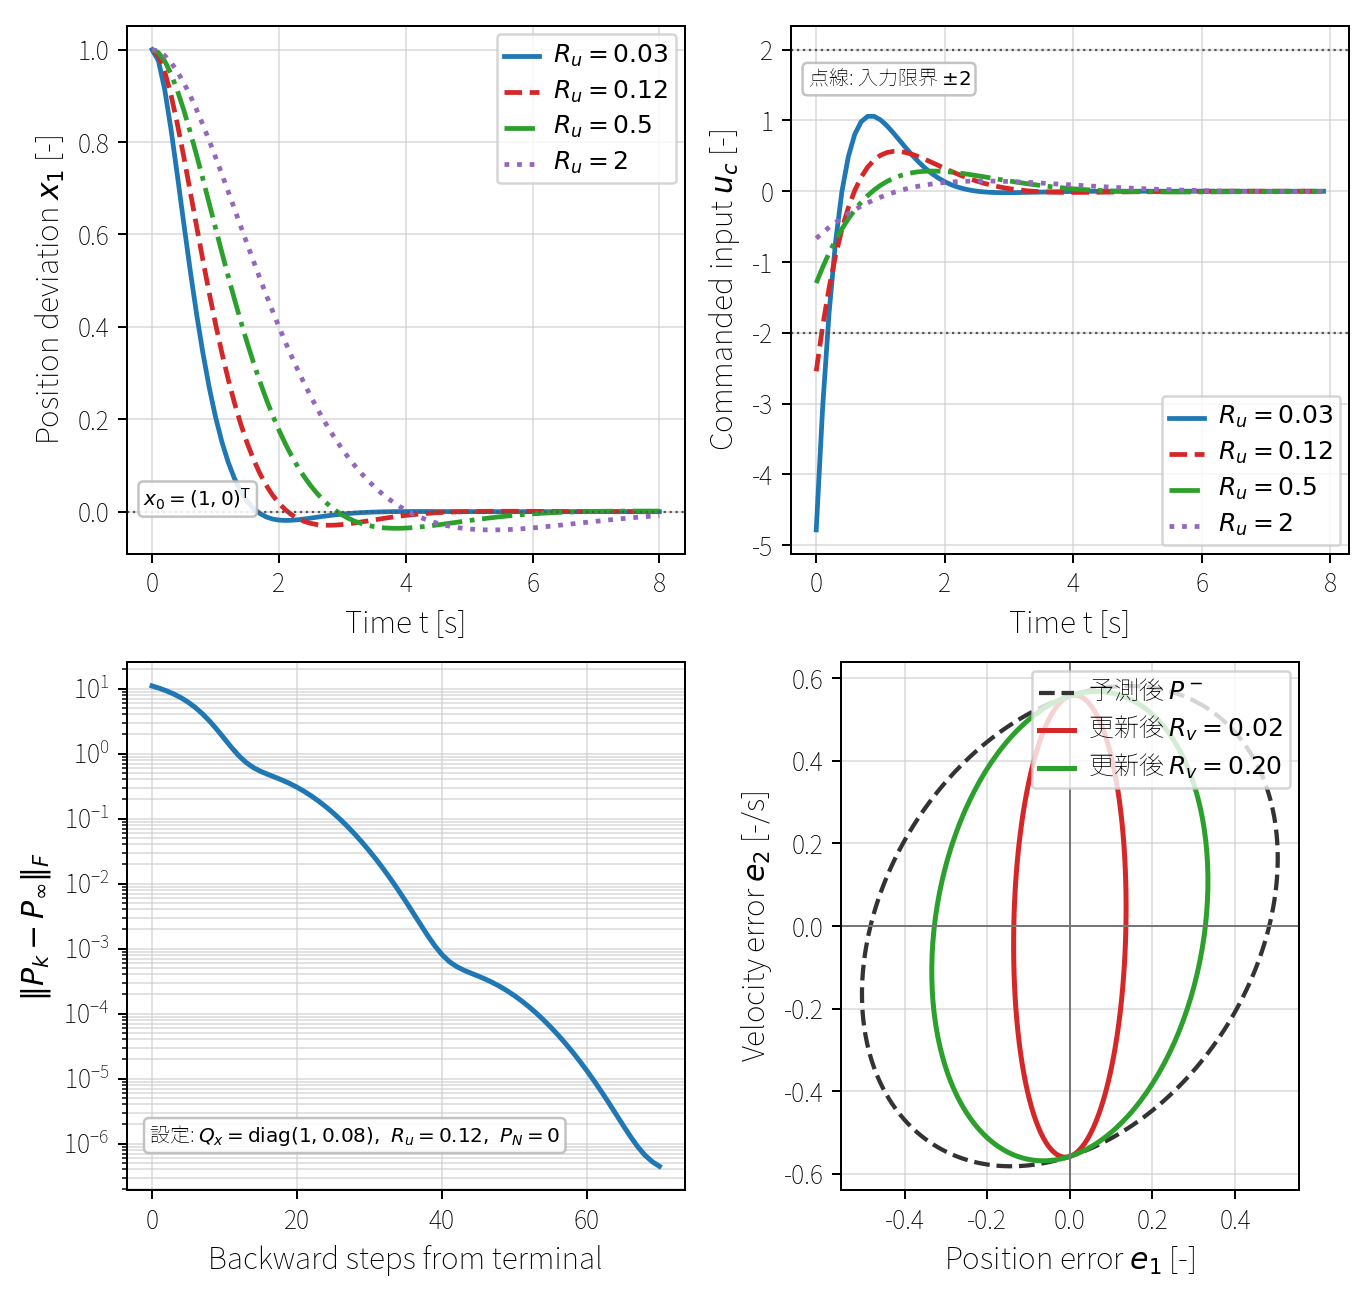
\includegraphics[width=0.95\linewidth,bb=0 0 1368 1296]{figures/lqr_kalman_examples.png}
\caption{二重積分器に対する LQR と Kalman フィルタの調整例。上段は入力重み $R_u$ による状態応答と入力指令の変化であり、入力限界を点線で示している。左下は有限ホライズンの後退リカッチ再帰が定常解へ近づく様子である。右下は予測後の誤差共分散楕円が位置測定によって更新される様子であり、測定ノイズ分散 $R_v$ が小さいほど測定方向の不確かさが強く縮む。}
\label{fig:lqr-kalman-examples}
\end{figure}

左下のリカッチ再帰では、終端条件から後ろ向きに計算した $P_k$ が定常解 $P_\infty$ に近づく。これはホライズンを長くしたとき、現在時刻から十分遠い終端条件の影響が薄れ、無限ホライズン LQR のゲインへ近づくことを表す。右下の共分散楕円は、予測で広がった不確かさが測定更新で縮む過程を示す。位置だけを測っているので、主に位置方向の幅が縮み、速度方向は状態方程式との相関を通じて間接的に修正される。$R_v$ を大きくすると測定を疑うため、更新後楕円は予測楕円に近く残る。

\begin{practice}[重みと共分散図の確認]
図\ref{fig:lqr-kalman-examples}を用いて、$R_u=0.03$ と $R_u=2$ の応答を比較せよ。整定の速さ、最大入力指令、入力限界を越える有無を評価し、実際の入力が飽和する場合に LQR の線形設計と閉ループシミュレーションの結果がずれる理由を説明せよ。さらに右下の共分散楕円について、$R_v$ を大きくしたとき Kalman ゲインが小さくなることを、楕円の縮み方と $K=P^-C^\T(CP^-C^\T+R_v)^{-1}$ から確認せよ。
\end{practice}

\subsection{連続時間 Kalman--Bucy フィルタ}

離散時間 Kalman フィルタでは、時刻 $k-1$ から $k$ へ進める予測と、時刻 $k$ の測定値による更新を分けて書いた。連続時間で測定が絶えず入ってくると考えると、この二段構造は微小時間ごとに連続して繰り返される極限になる。この極限で得られる線形ガウス推定器を Kalman--Bucy フィルタという。

状態を $x(t)\in\R^n$、入力を $u(t)\in\R^m$、測定を $y(t)\in\R^p$ とする。連続時間の線形確率モデルを、白色ノイズを形式的に用いて
\begin{align}
  \dot{x}(t)&=Ax(t)+Bu(t)+Gw(t),\\
  y(t)&=Cx(t)+v(t)
  \label{eq:kb-formal-model}
\end{align}
と書くことが多い。ここで $A\in\R^{n\times n}$、$B\in\R^{n\times m}$、$G\in\R^{n\times r}$、$C\in\R^{p\times n}$ である。$w(t)\in\R^r$ はプロセスノイズ、$v(t)\in\R^p$ は測定ノイズであり、
\begin{align}
  E[w(t)]&=0,
  &E[v(t)]&=0,\\
  E[w(t)w(\tau)^\T]&=Q_w\delta(t-\tau),
  &E[v(t)v(\tau)^\T]&=R_v\delta(t-\tau),\\
  E[w(t)v(\tau)^\T]&=0
\end{align}
を仮定する。$Q_w=Q_w^\T\ge0$ は $r\times r$ のプロセスノイズ強度、$R_v=R_v^\T>0$ は $p\times p$ の測定ノイズ強度である。$\delta(t-\tau)$ は Dirac のデルタであり、連続時間の白色ノイズが普通の関数ではなく、積分したときに有限の分散を持つ理想化であることを表す。

この理想化を少し丁寧に扱うには、独立な Wiener 過程 $\beta(t)\in\R^r$、$\eta(t)\in\R^p$ を用いて
\begin{align}
  \dd x(t)&=(Ax(t)+Bu(t))\,\dd t+G\,\dd\beta(t),\\
  \dd z(t)&=Cx(t)\,\dd t+\dd\eta(t)
  \label{eq:kb-stochastic-model}
\end{align}
と書く。$z(t)$ は測定信号を時間積分した量であり、形式的には $y(t)=\dd z(t)/\dd t$ と見れば \weq{kb-formal-model} に対応する。増分の共分散は
\begin{align}
  E[\dd\beta(t)\dd\beta(t)^\T]&=Q_w\,\dd t,\\
  E[\dd\eta(t)\dd\eta(t)^\T]&=R_v\,\dd t,\\
  E[\dd\beta(t)\dd\eta(t)^\T]&=0
\end{align}
である。以下では、初期推定誤差 $x(0)-\hat{x}(0)$ がこれらのノイズと無相関で、共分散
\begin{equation}
  P(0)=E[(x(0)-\hat{x}(0))(x(0)-\hat{x}(0))^\T]
\end{equation}
を持つとする。

Kalman--Bucy フィルタは、測定の予測誤差を連続時間で注入するオブザーバである。測定微分を用いると
\begin{equation}
  \dd\hat{x}(t)
  =(A\hat{x}(t)+Bu(t))\,\dd t
  +L(t)\{\dd z(t)-C\hat{x}(t)\,\dd t\}
  \label{eq:kb-filter-differential}
\end{equation}
であり、形式的な測定 $y(t)$ を用いれば
\begin{equation}
  \dot{\hat{x}}(t)
  =A\hat{x}(t)+Bu(t)+L(t)\{y(t)-C\hat{x}(t)\}
  \label{eq:kb-filter-formal}
\end{equation}
と書ける。$L(t)\in\R^{n\times p}$ は連続時間の Kalman ゲインである。$y-C\hat{x}$ は離散時間の場合の革新 $\nu_k=y_k-C_k\hat{x}_{k|k-1}$ に対応し、測定が予測より大きい方向へ状態推定を修正する信号である。

\begin{derivation}
推定誤差を
\begin{equation}
  e(t)=x(t)-\hat{x}(t)
\end{equation}
と置く。\weq{kb-stochastic-model} と \weq{kb-filter-differential} の差を取ると
\begin{align}
  \dd e
  &=\dd x-\dd\hat{x}\\
  &=(Ax+Bu)\,\dd t+G\,\dd\beta
    -(A\hat{x}+Bu)\,\dd t
    -L\{C(x-\hat{x})\,\dd t+\dd\eta\}\\
  &=(A-LC)e\,\dd t+G\,\dd\beta-L\,\dd\eta
  \label{eq:kb-error-dynamics}
\end{align}
を得る。入力 $u$ は既知として推定器にも入っているため、誤差方程式から消える。

誤差共分散を
\begin{equation}
  P(t)=E[e(t)e(t)^\T]\in\R^{n\times n}
\end{equation}
と定義する。微小変化では積の微分に二次のノイズ増分が残るので、Itô の積公式
\begin{equation}
  \dd(ee^\T)=(\dd e)e^\T+e(\dd e)^\T+(\dd e)(\dd e)^\T
\end{equation}
を使う。\weq{kb-error-dynamics} を代入して期待値を取ると、$e$ と新しいノイズ増分の交差項、および $\dd\beta$ と $\dd\eta$ の交差項は仮定により消える。残る項は
\begin{align}
  \dot{P}
  &=(A-LC)P+P(A-LC)^\T
    +GQ_wG^\T+LR_vL^\T\\
  &=AP+PA^\T+GQ_wG^\T
    -LCP-PC^\T L^\T+LR_vL^\T.
  \label{eq:kb-covariance-for-gain}
\end{align}
ここで $GQ_wG^\T$ はプロセスノイズが状態共分散を増やす項、$LR_vL^\T$ は測定ノイズをゲインで状態空間へ戻した項である。一方で $-LCP-PC^\T L^\T$ は、測定から得た情報が推定誤差を減らす効果を表す。

離散時間の場合と同じく、瞬間的な共分散の増え方を小さくする $L$ を選ぶ。記号を軽くするため $R=R_v$ と書くと、$L$ に依存する部分は
\begin{equation}
  -LCP-PC^\T L^\T+LRL^\T
\end{equation}
である。これを平方完成すると
\begin{align}
  -LCP-PC^\T L^\T+LRL^\T
  &=
  (L-PC^\T R^{-1})R(L-PC^\T R^{-1})^\T\\
  &\quad -PC^\T R^{-1}CP.
\end{align}
$R_v>0$ なので第一項は半正定値であり、最小にするゲインは
\begin{equation}
  L(t)=P(t)C^\T R_v^{-1}
  \label{eq:kb-gain}
\end{equation}
である。これを \weq{kb-covariance-for-gain} に代入すると、連続時間 Kalman--Bucy フィルタの共分散リカッチ方程式
\begin{equation}
  \dot{P}
  =AP+PA^\T+GQ_wG^\T
  -PC^\T R_v^{-1}CP,
  \qquad P(0)=P_0
  \label{eq:kb-riccati}
\end{equation}
を得る。
\end{derivation}

\weq{kb-riccati} は LQR のリカッチ方程式とよく似ている。LQR では入力を使って状態の増大を抑えるために $-PBR^{-1}B^\T P$ が現れた。Kalman--Bucy フィルタでは測定を使って推定誤差を抑えるために $-PC^\T R_v^{-1}CP$ が現れる。$GQ_wG^\T$ はモデルをどれだけ疑うか、$R_v$ は測定をどれだけ疑うかを表す。$Q_w$ を大きくすれば $P$ が大きくなりやすく、ゲイン $L=PC^\T R_v^{-1}$ は測定へ強く反応する。$R_v$ を大きくすれば、測定の信頼度が下がり、ゲインは小さくなる。

時不変で長時間運転する場合、条件がよければ $P(t)$ は定常値 $P_\infty$ に収束する。このとき
\begin{equation}
  0=AP_\infty+P_\infty A^\T+GQ_wG^\T
  -P_\infty C^\T R_v^{-1}CP_\infty
\end{equation}
を満たし、定常ゲインは
\begin{equation}
  L_\infty=P_\infty C^\T R_v^{-1}
\end{equation}
である。代表的な十分条件は、測定から不安定なモードを観測できるという可検出性と、プロセスノイズで励起される不確かさが安定化可能な範囲にあることである。すなわち、推定すべき不安定な動きが測定にまったく現れなければ、どれだけゲインを調整しても誤差を抑えられない。

離散時間 Kalman フィルタとの対応は、微小時間幅 $h$ で見ると分かりやすい。測定を無視してモデルだけで進めれば
\begin{align}
  \hat{x}(t+h)&=\hat{x}(t)+h(A\hat{x}(t)+Bu(t))+O(h^2),\\
  P(t+h)&=P(t)+h\{AP(t)+P(t)A^\T+GQ_wG^\T\}+O(h^2)
\end{align}
となり、これは離散時間の予測ステップに対応する。一方、同じ微小時間内に入る連続測定は、共分散を
\begin{equation}
  -h\,P(t)C^\T R_v^{-1}CP(t)
\end{equation}
だけ減らす方向に働く。したがって、離散時間の「予測してから更新する」という二段階は、連続時間では一つの微分方程式の中で同時に進む。数値実装では、\weq{kb-filter-differential} と \weq{kb-riccati} を時間刻みで積分するか、サンプリング周期 $h$ ごとに
\begin{align}
  A_d&=e^{Ah},\\
  B_d&=\int_0^h e^{A\sigma}B\,\dd\sigma,\\
  Q_d&=\int_0^h e^{A\sigma}GQ_wG^\T e^{A^\T\sigma}\,\dd\sigma
\end{align}
を用いて離散時間モデルへ変換し、前節の離散時間 Kalman フィルタを使う。

実用上は、連続時間の白色ノイズをそのまま物理信号と見なしてはいけない。白色ノイズは全周波数に同じ強度を持つ理想化であり、実際の外乱やセンサノイズには帯域、遅れ、量子化、フィルタ処理がある。また、サンプルされたセンサ値の分散 $R_s$ と、連続時間モデルの強度 $R_v$ は同じ量ではない。測定が区間平均なのか、瞬時値をサンプルしたものなのか、前段のアナログフィルタを通っているのかによって対応が変わる。連続モデルから実装へ移すときは、サンプリング周期、ノイズ強度の単位、離散化した $Q_d$ と測定共分散の意味をそろえる必要がある。熱系の温度推定のような低速の対象でも、モデル化していない熱流を $Q_w$ で表すのか、センサ読み取りのばらつきを $R_v$ または離散時間の $R_s$ で表すのかを分けて調整することが、フィルタの応答を評価する第一条件になる。

\subsection{LQG 制御と分離原理}

LQR は状態 $x$ が利用できるときの二次評価最適な入力を与え、Kalman フィルタは測定 $y$ から状態の条件付き平均を推定する。多くの制御対象では、速度、内部温度、ばねの伸び、電流の一部などが直接測れないため、状態フィードバック $u=-Kx$ はそのまま実装できない。そこで、測れる出力から $\hat{x}$ を作り、状態フィードバックの $x$ を $\hat{x}$ で置き換える。この構成を、線形二次ガウス制御、すなわち LQG 制御という。名称の Linear はモデルが線形であること、Quadratic は評価関数が二次形式であること、Gaussian はノイズと初期状態の確率モデルを正規分布で扱うことを表している。

連続時間の標準的な LQG 問題を
\begin{align}
  \dot{x}(t)&=Ax(t)+Bu(t)+Gw(t),\\
  y(t)&=Cx(t)+v(t)
  \label{eq:lqg-plant}
\end{align}
と置く。状態は $x\in\R^n$、入力は $u\in\R^m$、測定は $y\in\R^p$ である。$w$ はモデル化しない外乱や入力されない揺らぎを表すプロセスノイズ、$v$ は測定ノイズである。ここでは
\begin{align}
  E[w(t)]&=0,
  &E[v(t)]&=0,\\
  E[w(t)w(\tau)^\T]&=Q_w\delta(t-\tau),
  &E[v(t)v(\tau)^\T]&=R_v\delta(t-\tau),\\
  E[w(t)v(\tau)^\T]&=0
\end{align}
を仮定し、$Q_w=Q_w^\T\ge0$、$R_v=R_v^\T>0$ とする。初期状態の推定誤差も、これらのノイズと無相関であると仮定する。制御性能は、有限ホライズンなら
\begin{equation}
  J_T
  =E\left[
    x(T)^\T S x(T)
    +\int_0^T
      \{x(t)^\T Q_x x(t)+u(t)^\T R_u u(t)\}\,\dd t
  \right]
  \label{eq:lqg-finite-cost}
\end{equation}
で評価する。ここで $Q_x=Q_x^\T\ge0$、$R_u=R_u^\T>0$、$S=S^\T\ge0$ であり、$Q_x$ は状態偏差への重み、$R_u$ は入力への重みである。プロセスノイズが持続的に入る無限ホライズンでは、単純な積分型の期待コストは一般に時間とともに増え続けるため、定常運転の評価には
\begin{equation}
  \bar{J}
  =
  \limsup_{T\to\infty}
  \frac{1}{T}
  E\int_0^T
    \{x(t)^\T Q_x x(t)+u(t)^\T R_u u(t)\}\,\dd t
  \label{eq:lqg-average-cost}
\end{equation}
のような平均コストを用いる。初期値だけを減衰させる決定論的 LQR と、持続的なノイズを受ける LQG では、この点で評価の意味が異なる。

LQG の制御器は、制御用リカッチ方程式と推定用リカッチ方程式を別々に解いて作る。有限ホライズンの制御側では
\begin{equation}
  -\dot{P}_c
  =
  A^\T P_c+P_cA-P_cBR_u^{-1}B^\T P_c+Q_x,
  \qquad
  P_c(T)=S
  \label{eq:lqg-control-rde}
\end{equation}
を解き、
\begin{equation}
  K(t)=R_u^{-1}B^\T P_c(t)
  \label{eq:lqg-control-gain}
\end{equation}
とする。無限ホライズンで定常ゲインを使う場合は、対応する代数リカッチ方程式
\begin{equation}
  A^\T P_c+P_cA-P_cBR_u^{-1}B^\T P_c+Q_x=0
  \label{eq:lqg-control-care}
\end{equation}
の安定化解から $K=R_u^{-1}B^\T P_c$ を得る。一方、推定側では Kalman--Bucy フィルタの共分散リカッチ方程式
\begin{equation}
  \dot{P}_e
  =
  AP_e+P_eA^\T+GQ_wG^\T
  -P_eC^\T R_v^{-1}CP_e
  \label{eq:lqg-estimator-rde}
\end{equation}
を用い、
\begin{equation}
  L(t)=P_e(t)C^\T R_v^{-1}
  \label{eq:lqg-estimator-gain}
\end{equation}
とする。定常推定器では
\begin{equation}
  0=
  AP_e+P_eA^\T+GQ_wG^\T
  -P_eC^\T R_v^{-1}CP_e
  \label{eq:lqg-estimator-care}
\end{equation}
の安定化解を使う。制御側の $P_c$ は将来の制御コストを表し、推定側の $P_e$ は推定誤差の共分散を表す。同じリカッチ方程式という名前で呼ばれても、二つの行列が表す量は異なる。

得られた LQG 制御器は
\begin{align}
  \dot{\hat{x}}&=A\hat{x}+Bu+L(y-C\hat{x}),\\
  u&=-K\hat{x}
  \label{eq:lqg-controller}
\end{align}
である。$y-C\hat{x}$ は測定の革新であり、推定器はこの革新を用いて $\hat{x}$ を修正する。制御入力は、推定値 $\hat{x}$ を真の状態であるかのように扱って LQR ゲインを掛ける。この性質を確定性等価性という。確定性等価性は、「不確かさを無視してよい」という意味ではない。ノイズ共分散は推定器の $L$ を決め、推定誤差は閉ループの入力変動や状態変動として現れる。ただし、最適な制御則の形は、完全状態が測れる LQR の $x$ を条件付き平均 $\hat{x}$ に置き換えたものになる。

図\ref{fig:lqg-signal-path}は、この式を信号経路として並べたものである。制御器が計算する信号を入力指令 $u_c=-K\hat{x}$、アクチュエータを通って対象へ実際に入る信号を $u_a$ と区別している。線形 LQG の導出では $u_a=u_c$ を仮定するが、飽和やレート制限が入る実装では $u_a$ が推定器にも渡される既知入力でなければならない。推定器が $u_c$ を使い続けると、対象に入った入力との不一致が推定誤差として蓄積し、分離原理の前提から外れる。

\begin{figure}[tb]
\centering
\setlength{\unitlength}{1mm}
\begin{picture}(136,68)
\small
\put(16,44){\framebox(34,12){\shortstack{制御器\\$u_c=-K\hat{x}$}}}
\put(58,44){\framebox(30,12){\shortstack{飽和・駆動\\$u_a$}}}
\put(98,44){\framebox(28,12){\shortstack{対象\\$x$}}}
\put(98,14){\framebox(28,12){\shortstack{測定\\$y=Cx+v$}}}
\put(16,14){\framebox(34,12){\shortstack{推定器\\$\hat{x}$}}}
\put(50,50){\vector(1,0){8}}
\put(51,53){$u_c$}
\put(88,50){\vector(1,0){10}}
\put(90,53){$u_a$}
\put(112,65){\vector(0,-1){9}}
\put(114,60){$w$}
\put(112,44){\vector(0,-1){18}}
\put(115,35){$x$}
\put(132,20){\vector(-1,0){6}}
\put(129,22){$v$}
\put(98,20){\vector(-1,0){48}}
\put(74,22){$y$}
\put(33,26){\vector(0,1){18}}
\put(35,34){$\hat{x}$}
\put(73,44){\line(0,-1){12}}
\put(73,32){\vector(-1,0){28}}
\put(45,32){\vector(0,-1){6}}
\put(50,34){既知入力 $u_a$}
\end{picture}
\caption{LQG 制御の信号経路。測定 $y$ から推定器が $\hat{x}$ を作り、制御器が入力指令 $u_c$ を計算し、飽和や駆動系を通った実入力 $u_a$ が対象へ入る。線形導出では $u_a=u_c$ とみなすが、飽和がある場合は実入力を推定器の既知入力として扱う。}
\label{fig:lqg-signal-path}
\end{figure}

この置き換えが成立する理由は、条件付き平均と推定誤差の直交性にある。時刻 $t$ までの測定履歴を $\mathcal{Y}_t$ とし、
\begin{equation}
  \hat{x}(t)=E[x(t)\mid\mathcal{Y}_t],
  \qquad
  e(t)=x(t)-\hat{x}(t)
\end{equation}
と置く。条件付き平均の定義より
\begin{equation}
  E[e(t)\mid\mathcal{Y}_t]=0
\end{equation}
である。したがって、状態重みの条件付き期待値は
\begin{align}
  E[x^\T Q_x x\mid\mathcal{Y}_t]
  &=
  E[(\hat{x}+e)^\T Q_x(\hat{x}+e)\mid\mathcal{Y}_t]\\
  &=
  \hat{x}^\T Q_x\hat{x}
  +2\hat{x}^\T Q_x E[e\mid\mathcal{Y}_t]
  +E[e^\T Q_x e\mid\mathcal{Y}_t]\\
  &=
  \hat{x}^\T Q_x\hat{x}
  +\tr(Q_xP_e(t)).
  \label{eq:lqg-cost-decomposition}
\end{align}
最後の等号では $P_e(t)=E[ee^\T\mid\mathcal{Y}_t]$ と、$E[e^\T Q_x e]=\tr(Q_x E[ee^\T])$ を使った。右辺の第一項だけが、現在の推定値を状態として見た LQR の状態コストである。第二項は推定誤差から避けられずに生じるコストであり、線形ガウスモデルと既知入力の仮定のもとでは、推定誤差共分散の時間発展は制御入力の選び方に依存しない。入力コスト $u^\T R_u u$ はそのまま制御側に残るので、制御の最適化は $\hat{x}$ を状態とする LQR と同じ形になる。これが LQG における分離原理の中身である。

\begin{theorem}[LQG の分離原理]
線形モデル \weq{lqg-plant}、二次評価 \weq{lqg-finite-cost}、ゼロ平均の独立なガウスノイズ、既知入力、および初期推定誤差とノイズの独立性を仮定する。制御側リカッチ方程式と推定側リカッチ方程式がそれぞれ適切な解を持つなら、最適な出力フィードバック制御器は Kalman フィルタと LQR 状態フィードバックを
\begin{equation}
  u(t)=-K(t)\hat{x}(t)
\end{equation}
で直列に接続した形で与えられる。定常無限ホライズンでは、$(A,B)$ の可安定性、$(A,Q_x^{1/2})$ の可検出性、$(A,C)$ の可検出性、および $W=GQ_wG^\T$ に対する $(A,W^{1/2})$ の可安定性が代表的な十分条件である。
\end{theorem}

分離原理という名前は、閉ループの状態方程式にも直接現れる。推定誤差を
\begin{equation}
  e=x-\hat{x}
\end{equation}
と置き、定常ゲイン $K,L$ を用いると
\begin{align}
  \dot{x}
  &=Ax+B(-K\hat{x})+Gw\\
  &=(A-BK)x+BKe+Gw,
\end{align}
であり、推定誤差は
\begin{align}
  \dot{e}
  &=\dot{x}-\dot{\hat{x}}\\
  &=(A-LC)e+Gw-Lv
\end{align}
を満たす。したがって、拡大状態 $(x,e)$ に対する閉ループは
\begin{equation}
  \begin{bmatrix}
    \dot{x}\\
    \dot{e}
  \end{bmatrix}
  =
  \begin{bmatrix}
    A-BK & BK\\
    0 & A-LC
  \end{bmatrix}
  \begin{bmatrix}
    x\\
    e
  \end{bmatrix}
  +
  \begin{bmatrix}
    G & 0\\
    G & -L
  \end{bmatrix}
  \begin{bmatrix}
    w\\
    v
  \end{bmatrix}.
  \label{eq:lqg-augmented-dynamics}
\end{equation}
係数行列はブロック上三角である。ノイズを 0 として平均の安定性だけを見ると、その固有値は $A-BK$ の固有値と $A-LC$ の固有値を合わせたものになる。したがって、LQR で $A-BK$ を Hurwitz にし、Kalman--Bucy フィルタで $A-LC$ を Hurwitz にすれば、平均的な閉ループは安定になる。さらにノイズ強度が有限で、両方の行列が Hurwitz なら、拡大系の共分散も定常値へ収束し、状態と推定誤差の二乗平均は有界に保たれる。

調整の解釈は二組に分けると整理しやすい。$Q_x$ と $R_u$ は、制御として何を優先するかを決める。$Q_x$ を大きくすると状態偏差を強く抑えるため $K$ が大きくなりやすく、応答は速くなる一方で入力の振れや飽和の危険が増える。$R_u$ を大きくすると入力を節約し、応答は穏やかになる。これに対し、$Q_w$ と $R_v$ は、推定器がモデルと測定のどちらを信じるかを決める。$Q_w$ を大きくすると、モデル化しない外乱が大きいと見なされ、推定器は測定の革新へ強く反応する。$R_v$ を大きくすると、測定値を疑うため $L$ は小さくなり、推定値はモデル予測に近づく。たとえば熱系で室温を制御する場合、外気や人の出入りによる未モデル化熱流が大きいなら $Q_w$ を増やし、温度センサのばらつきや量子化が大きいなら $R_v$ を増やす。入力重み $R_u$ はヒータ出力の制限や消費電力に対応し、状態重み $Q_x$ は温度偏差をどれだけ早く戻したいかに対応する。

ただし、分離して設計できることと、相互作用を確認しなくてよいことは同じではない。$K$ が大きいと、推定値に含まれる高周波の測定ノイズ成分が入力へ強く入る。$L$ が大きいと、推定値は測定に素早く追従するが、センサノイズにも敏感になる。入力飽和、レート制限、むだ時間、非線形性、モデル誤差、ノイズの相関、非ガウス分布、センサの帯域制限があると、上の分離原理の仮定から外れる。特に入力が飽和すると、推定器が仮定している既知入力 $u$ と実際に対象へ入った入力がずれ、推定誤差の独立なリカッチ方程式という構造が崩れる。LQG は線形ガウスモデルに対する基準設計として強力であるが、最終的な設計では飽和を含む閉ループシミュレーション、ノイズ共分散の妥当性確認、革新系列の白色性、入力の実効範囲、モデル誤差に対する感度を確認する必要がある。

離散時間でも同じ構造が成り立つ。離散時間 LQR のリカッチ方程式から $K_k$ を求め、離散時間 Kalman フィルタから $\hat{x}_{k|k}$ を求めて
\begin{equation}
  u_k=-K_k\hat{x}_{k|k}
\end{equation}
とすればよい。実装では、サンプリング周期、ゼロ次ホールドで離散化した $A_d,B_d,Q_d$、測定時刻、計算遅れをそろえる。連続時間の式で設計したゲインをそのままデジタル制御器へ入れるのではなく、実際のサンプル周期で推定と制御がどの順序で実行されるかを明示することが、LQG を実機へ移すときの第一条件である。

\subsection{固定区間平滑化と RTS 平滑化}

Kalman フィルタの推定値 $\hat{x}_{k|k}$ は、時刻 $k$ までの測定履歴 $\mathcal{Y}_k$ を使った推定である。実時間制御では未来の測定値を待てないため、この片方向の推定が自然である。一方、実験後のデータ解析、軌道再構成、パラメータ同定、センサログの補正では、区間全体の測定値
\begin{equation}
  \mathcal{Y}_N=\{y_0,y_1,\ldots,y_N\}
\end{equation}
がすでに手元にある。このとき、時刻 $k<N$ の状態を推定するために $y_{k+1},\ldots,y_N$ も使える。区間 $0,\ldots,N$ 全体の測定値を用いて $x_k$ を推定する処理を固定区間平滑化という。表記として
\begin{equation}
  \hat{x}_{k|N}=E[x_k\mid\mathcal{Y}_N],
  \qquad
  P_{k|N}=E[(x_k-\hat{x}_{k|N})(x_k-\hat{x}_{k|N})^\T\mid\mathcal{Y}_N]
\end{equation}
を用いる。

平滑化はフィルタリングの否定ではなく、フィルタリングに未来側の情報を後から戻す操作である。熱系で例えれば、時刻 $k$ の温度推定は、その時刻までのセンサ値だけでなく、その後の温度の上がり方や下がり方からも制約を受ける。後で温度が急に上がったなら、時刻 $k$ の未モデル化熱流がすでに始まっていた可能性が高い。固定区間平滑化は、このような「後で分かった整合条件」をモデルの時間発展を通じて過去へ伝える。

代表的な線形ガウス平滑化が Rauch--Tung--Striebel 平滑化、すなわち RTS 平滑化である。離散時間モデルを
\begin{equation}
  x_{k+1}=A_kx_k+B_ku_k+G_kw_k
\end{equation}
とし、前向きの Kalman フィルタで
\begin{equation}
  \hat{x}_{k|k},
  \quad
  P_{k|k},
  \quad
  \hat{x}_{k+1|k},
  \quad
  P_{k+1|k}
\end{equation}
を保存しておく。ここで
\begin{align}
  \hat{x}_{k+1|k}
  &=A_k\hat{x}_{k|k}+B_ku_k,\\
  P_{k+1|k}
  &=A_kP_{k|k}A_k^\T+G_kQ_{w,k}G_k^\T
\end{align}
である。終端では、未来の測定値がもうないので
\begin{equation}
  \hat{x}_{N|N}
  \quad\text{と}\quad
  P_{N|N}
\end{equation}
をそのまま平滑化の初期値として用いる。すなわち
\begin{equation}
  \hat{x}_{N|N}^{\mathrm{s}}=\hat{x}_{N|N},
  \qquad
  P_{N|N}^{\mathrm{s}}=P_{N|N}
\end{equation}
と書く。ただし上付き $\mathrm{s}$ は平滑化後の量を表す記号であり、以下では
\begin{equation}
  \hat{x}_{k|N}=\hat{x}_{k|N}^{\mathrm{s}},
  \qquad
  P_{k|N}=P_{k|N}^{\mathrm{s}}
\end{equation}
と同じ意味で使う。

RTS 平滑化では、$k=N-1,N-2,\ldots,0$ と時間を逆向きに進める。平滑化ゲインを
\begin{equation}
  J_k=P_{k|k}A_k^\T P_{k+1|k}^{-1}
  \label{eq:rts-smoother-gain}
\end{equation}
と置くと、平均と共分散は
\begin{align}
  \hat{x}_{k|N}
  &=
  \hat{x}_{k|k}
  +J_k(\hat{x}_{k+1|N}-\hat{x}_{k+1|k}),
  \label{eq:rts-smoother-mean}\\
  P_{k|N}
  &=
  P_{k|k}
  +J_k(P_{k+1|N}-P_{k+1|k})J_k^\T
  \label{eq:rts-smoother-covariance}
\end{align}
で更新される。\weq{rts-smoother-mean} の括弧
\begin{equation}
  \hat{x}_{k+1|N}-\hat{x}_{k+1|k}
\end{equation}
は、時刻 $k+1$ の状態について、未来の測定値を含めた推定が前向き予測からどれだけずれたかを表す。このずれを、$x_k$ と $x_{k+1}$ の相関を表す係数 $J_k$ で時刻 $k$ へ戻す。共分散式 \weq{rts-smoother-covariance} では、未来の測定値を使うことで $P_{k+1|N}$ が通常 $P_{k+1|k}$ より小さくなるため、その減少分が $J_k$ を通じて $P_{k|k}$ から差し引かれる。

\weq{rts-smoother-gain} は逆行列を明示しているが、実装では $P_{k+1|k}^{-1}$ を直接作らない。線形方程式
\begin{equation}
  P_{k+1|k}X^\T=A_kP_{k|k}
\end{equation}
を Cholesky 分解や対称正定値用の解法で解き、$J_k=X$ とする。$P_{k+1|k}$ が特異に近い場合は、プロセスノイズの設定、モデルの可観測性、状態の単位スケーリングを見直す必要がある。平滑化は未来情報を使うため、実時間フィードバック制御器の中にはそのまま入れられない。固定遅れ平滑化のように数サンプルだけ遅らせる実装もあるが、遅れを許せない制御ループでは、平滑化は主にログ解析や推定器調整のための手段になる。

\subsection{情報形式の Kalman フィルタ}

共分散形式の Kalman フィルタは、推定誤差共分散 $P$ と推定平均 $\hat{x}$ を主変数にする。これに対して、情報形式の Kalman フィルタは
\begin{equation}
  Y=P^{-1},
  \qquad
  \eta=Y\hat{x}
  \label{eq:information-state}
\end{equation}
を主変数にする。$Y$ を情報行列、$\eta$ を情報ベクトルという。$P$ が大きいことは不確かさが大きいことを意味するので、その逆行列 $Y$ は状態についてどれだけ情報を持っているかを表す。推定値そのものは
\begin{equation}
  \hat{x}=Y^{-1}\eta
\end{equation}
で戻せるが、数値実装ではこの逆行列も直接作らず、線形方程式
\begin{equation}
  Y\hat{x}=\eta
\end{equation}
を解く。

情報形式の利点は、測定更新が加算で書けることである。時刻 $k$ の予測情報を $Y_{k|k-1}$、$\eta_{k|k-1}$ とし、測定モデルを
\begin{equation}
  y_k=C_kx_k+v_k,
  \qquad
  v_k\sim(0,R_{v,k})
\end{equation}
とする。測定を得た後の情報行列と情報ベクトルは
\begin{align}
  Y_{k|k}
  &=
  Y_{k|k-1}+C_k^\T R_{v,k}^{-1}C_k,
  \label{eq:information-update-matrix}\\
  \eta_{k|k}
  &=
  \eta_{k|k-1}+C_k^\T R_{v,k}^{-1}y_k.
  \label{eq:information-update-vector}
\end{align}
この式は、ガウス分布の指数部を足し合わせるだけで導ける。予測分布が
\begin{equation}
  p(x_k\mid\mathcal{Y}_{k-1})
  \propto
  \exp\left[
    -\frac{1}{2}x_k^\T Y_{k|k-1}x_k
    +\eta_{k|k-1}^\T x_k
  \right]
\end{equation}
であり、測定尤度が
\begin{equation}
  p(y_k\mid x_k)
  \propto
  \exp\left[
    -\frac{1}{2}(y_k-C_kx_k)^\T R_{v,k}^{-1}(y_k-C_kx_k)
  \right]
\end{equation}
であるとする。$x_k$ に依存する項だけを集めると
\begin{align}
  &-\frac{1}{2}x_k^\T Y_{k|k-1}x_k+\eta_{k|k-1}^\T x_k\\
  &\quad
  -\frac{1}{2}x_k^\T C_k^\T R_{v,k}^{-1}C_kx_k
  +x_k^\T C_k^\T R_{v,k}^{-1}y_k
\end{align}
となる。二次項の係数と一次項の係数を読み取れば、\weq{information-update-matrix} と \weq{information-update-vector} が得られる。測定値だけに依存する定数項は正規化定数に吸収される。

複数の独立なセンサが同じ時刻に入る場合、この加算性はさらに明確になる。センサ $i$ が
\begin{equation}
  y_k^{(i)}=C_k^{(i)}x_k+v_k^{(i)},
  \qquad
  E[v_k^{(i)}(v_k^{(j)})^\T]=0\quad(i\ne j)
\end{equation}
を満たすなら、
\begin{align}
  Y_{k|k}
  &=
  Y_{k|k-1}
  +\sum_i (C_k^{(i)})^\T
    (R_{v,k}^{(i)})^{-1}C_k^{(i)},\\
  \eta_{k|k}
  &=
  \eta_{k|k-1}
  +\sum_i (C_k^{(i)})^\T
    (R_{v,k}^{(i)})^{-1}y_k^{(i)}
\end{align}
でよい。したがって、センサが非同期に届く場合でも、その測定に対応する情報だけを順に足せる。$C_k^{(i)}$ が状態ベクトルの一部だけを見る疎な行列であれば、各センサが加える情報行列も疎になる。大規模な温度場、電力網、移動体群、SLAM のように、全状態のうち局所的な組だけを各測定が結びつける問題では、共分散行列 $P$ が密になりやすい一方で、情報行列 $Y$ やその Cholesky 因子は疎構造を保てることがある。この性質により、疎行列用の順序付け、疎 Cholesky 分解、局所測定の逐次追加が使いやすくなる。

時間予測は、測定更新ほど単純な加算にはならない。線形モデル
\begin{equation}
  x_k=A_{k-1}x_{k-1}+B_{k-1}u_{k-1}+q_{k-1},
  \qquad
  q_{k-1}\sim(0,Q_{k-1})
\end{equation}
を用いるなら、共分散形式では
\begin{align}
  \hat{x}_{k|k-1}
  &=A_{k-1}\hat{x}_{k-1|k-1}+B_{k-1}u_{k-1},\\
  P_{k|k-1}
  &=A_{k-1}P_{k-1|k-1}A_{k-1}^\T+Q_{k-1}
\end{align}
を計算してから
\begin{equation}
  Y_{k|k-1}=P_{k|k-1}^{-1},
  \qquad
  \eta_{k|k-1}=Y_{k|k-1}\hat{x}_{k|k-1}
  \label{eq:information-prediction-vector}
\end{equation}
とすればよい。ここでも $\hat{x}_{k|k-1}=Y_{k|k-1}^{-1}\eta_{k|k-1}$ を取り出す場面では逆行列を明示的に作らず、線形方程式 $Y_{k|k-1}\hat{x}_{k|k-1}=\eta_{k|k-1}$ を解く。情報形式だけで表す場合も Woodbury の公式により
\begin{equation}
  Y_{k|k-1}
  =
  Q_{k-1}^{-1}
  -Q_{k-1}^{-1}A_{k-1}
  (Y_{k-1|k-1}+A_{k-1}^\T Q_{k-1}^{-1}A_{k-1})^{-1}
  A_{k-1}^\T Q_{k-1}^{-1}
  \label{eq:information-prediction-matrix}
\end{equation}
と書ける。ただし、この式は $Q_{k-1}$ が正定値であることを仮定しており、数値的には内側の線形方程式を疎分解で解く形で実装する。入力 $B_{k-1}u_{k-1}$ は平均を平行移動する項なので、情報ベクトルの予測では予測平均を通じて反映される。実装上は、予測段階を共分散形式または平方根形式で行い、測定更新だけを情報形式で疎に処理する混合構成も多い。重要なのは、どの形式でも同じ条件付きガウス分布を表しており、問題の疎性、センサ数、必要な出力が平均なのか共分散なのかに応じて表現を選ぶことである。

\subsection{数値安定性を保つ Kalman フィルタ実装}

Kalman フィルタの式は短いが、有限精度計算では共分散行列の対称性、半正定値性、条件数を保つことが設計の一部になる。共分散 $P$ は本来
\begin{equation}
  P=P^\T,
  \qquad
  z^\T Pz\ge0\quad(\forall z)
\end{equation}
を満たす。しかし、簡略形
\begin{equation}
  P_{k|k}=(I-K_kC_k)P_{k|k-1}
\end{equation}
をそのまま浮動小数点で計算すると、丸め誤差により $P_{k|k}$ がわずかに非対称になったり、負の固有値を持ったりすることがある。負の分散は確率モデルとして意味を持たず、次の Cholesky 分解やゲイン計算を破綻させる。

第一の実装原則は、共分散更新に Joseph 形式を使うことである。
\begin{equation}
  P_{k|k}
  =(I-K_kC_k)P_{k|k-1}(I-K_kC_k)^\T+K_kR_{v,k}K_k^\T
  \label{eq:stable-joseph-form}
\end{equation}
右辺は、半正定値行列を左右から掛けた項と、測定ノイズ共分散をゲインで写した項の和である。したがって、$P_{k|k-1}\ge0$、$R_{v,k}>0$ なら、数学的には $P_{k|k}\ge0$ が保たれる。簡略形と代数的には同じでも、Joseph 形式は丸め誤差に対して共分散の構造を壊しにくい。

第二の原則は、逆行列を明示的に作らないことである。Kalman ゲインを
\begin{equation}
  K_k=P_{k|k-1}C_k^\T S_k^{-1},
  \qquad
  S_k=C_kP_{k|k-1}C_k^\T+R_{v,k}
\end{equation}
と書いても、実装では $S_k^{-1}$ を計算しない。$S_k$ が対称正定値なら Cholesky 分解
\begin{equation}
  S_k=L_kL_k^\T
\end{equation}
を行い、三角行列の連立一次方程式を二回解いて $K_k$ を得る。$S_k$ の Cholesky 分解が失敗する場合、測定ノイズ共分散 $R_{v,k}$ が正定値になっていない、$P_{k|k-1}$ の半正定値性が崩れている、または状態や測定のスケーリングが悪い可能性がある。

第三の原則は、平方根形式を使って共分散そのものではなく因子を更新することである。たとえば
\begin{equation}
  P_{k|k}=S_{k|k}S_{k|k}^\T
\end{equation}
を保ちながら、$S_{k|k}$ を QR 分解や Cholesky 更新で計算する。予測段階では、行列
\begin{equation}
  \begin{bmatrix}
    A_{k-1}S_{k-1|k-1} & G_{k-1}Q_{w,k-1}^{1/2}
  \end{bmatrix}
\end{equation}
の積から $P_{k|k-1}$ を作る代わりに、この横長行列の転置に QR 分解を適用して $S_{k|k-1}$ を得る。測定更新でも、革新共分散や事後共分散の平方根を QR 分解で更新できる。平方根形式では、半正定値性が因子の積として表されるため、丸め誤差で小さな負の固有値が出る危険が減る。情報形式でも同様に
\begin{equation}
  Y_{k|k}=R_{k|k}^\T R_{k|k}
\end{equation}
のような平方根情報形式を使えば、疎 Cholesky 分解と相性がよい。

第四の原則は、対称化と条件数の監視を明示的に行うことである。計算後の共分散は
\begin{equation}
  P\leftarrow\frac{1}{2}(P+P^\T)
\end{equation}
で対称化してから次のステップへ渡すと、丸めによる反対称成分を抑えられる。さらに、$Q_w$、$R_v$、$P_0$ は対称行列として入力し、必要なら
\begin{equation}
  Q_w\leftarrow\frac{1}{2}(Q_w+Q_w^\T),
  \qquad
  R_v\leftarrow\frac{1}{2}(R_v+R_v^\T)
\end{equation}
と確認する。$R_v$ は通常正定値であるべきなので、分散が 0 に近い測定を完全に信じる設定は避け、小さな正の下限を置く。$Q_w$ は半正定値でもよいが、モデルが実際より硬すぎると $P$ が過小になり、革新に対して不自然に鈍い推定器になる。共分散の固有値を無理に切り上げる処理は最後の保護としては使えるが、それを常用しなければ動かない場合は、ノイズ共分散、離散化、単位スケーリング、観測モデルのいずれかを見直すべきである。

状態のスケーリングも数値安定性に直結する。位置をメートル、角度をラジアン、温度を摂氏、電流をアンペアで混在させること自体は自然だが、それらの典型値が $10^{-6}$ と $10^6$ のように大きく離れると、$P$ や $S_k$ の条件数が悪くなる。状態を無次元化する、代表値で割って同程度の大きさにする、重みや共分散をそのスケールに合わせて変換する、といった処理は、理論式を変えるのではなく、同じ推定問題を計算しやすい座標で解く操作である。

最後に、数値的に安定な実装であっても、統計的に妥当な推定になっているとは限らない。革新
\begin{equation}
  \nu_k=y_k-C_k\hat{x}_{k|k-1}
\end{equation}
と革新共分散 $S_k$ を使い、正規化革新二乗
\begin{equation}
  \epsilon_k=\nu_k^\T S_k^{-1}\nu_k
\end{equation}
を監視すると、$Q_w$ と $R_v$ の設定が極端でないかを調べられる。$\epsilon_k$ が継続的に大きすぎるなら、モデルが外乱を過小評価している、測定ノイズを小さく見積もりすぎている、またはモデル構造がずれている可能性がある。逆に小さすぎる状態が続くなら、共分散を過大に見積もっている可能性がある。Joseph 形式、平方根形式、疎な情報形式は計算を壊れにくくするための方法であり、革新系列の確認は確率モデルそのものを検査するための方法である。

\section{非線形系と力学モデリング}

\subsection{非線形系への拡張}

線形系では、応答、安定性、状態フィードバック、オブザーバ、LQR、カルマンフィルタが一つの流れとしてつながった。しかし、同じ線形モデルを対象の全領域へそのまま広げると、すぐに限界が現れる。小角の振子では $\sin\theta\simeq\theta$ と見なせるが、大きく振れた振子や上向き平衡点の近くでは、重力トルクの傾きも安定性の性質も小角モデルとは異なる。タンクの流出は水位差に比例するのではなく、典型的には水位の平方根に依存するため、ある水位で合わせた一次モデルは水位が大きく変わると流量予測にずれを生じる。アクチュエータが飽和する系では、設計上の入力をいくら大きくしても実際の力やトルクは上限で止まり、線形モデルが仮定した比例関係が崩れる。

小角近似の限界は、数値だけでも確認できる。表\ref{tab:pendulum-smallangle-check}は、下向き振子の重力項で使う $\sin\theta$ を $\theta$ で置き換えたときの相対誤差を示す。
\begin{table}[tbp]
  \centering
  \caption{振子の小角近似 $\sin\theta\simeq\theta$ の数値確認。この表は、角度偏差が大きくなるほど局所線形モデルの重力トルク予測が崩れることを示すが、この誤差だけで閉ループの安定領域や入力飽和の有無までは判定できない。}
  \label{tab:pendulum-smallangle-check}
  \begin{tabular}{c|c|c|c}
    $\theta$ [rad] & $\sin\theta$ & 近似値 $\theta$ & 相対誤差 [\%]\\
    \hline
    0.087 & 0.087 & 0.087 & 0.13\\
    0.524 & 0.500 & 0.524 & 4.5\\
    1.047 & 0.866 & 1.047 & 17.3\\
    1.571 & 1.000 & 1.571 & 36.3
  \end{tabular}
\end{table}
この確認から分かるのは、線形化が「小さい偏差で一次項が支配的」という条件つきの近似だという点である。$0.087$ rad 程度では重力項のずれはほとんど見えないが、$1.047$ rad では入力トルク計算に使う重力補償が約 $17$ \% ずれ、$1.571$ rad では三分の一を超える。したがって、線形章で得た極配置や LQR の式を使う場合でも、どの角度範囲でその接線モデルを信じるのかを本文中で明示しなければならない。

この限界は、線形制御を破棄すべきことを意味しない。必要なのは、まず対象が実際にどの変数で動き、入力、外乱、測定量、制約がどのように関係するかを非線形モデルとして書き、そのうえでどの動作点または基準軌道の近くを扱うのかを明示することである。近似を使う場合は、関数がその近傍で十分滑らかであること、偏差が小さいこと、入力飽和や接触切替のような不連続が支配的でないことを仮定する。この仮定のもとでだけ、偏差変数、接平面、ヤコビアンによる一次近似が、前章までの線形系の設計法へ接続する。

\subsubsection{非線形状態方程式と出力方程式}

この目的のため、連続時間の非線形状態空間モデルを
\begin{align}
  \dot{x}&=f(x,u),\\
  y&=h(x,u)
\end{align}
と書く。ここで $x(t)\in\R^n$ は状態、$u(t)\in\R^m$ は入力、$y(t)\in\R^p$ は出力である。$f:\R^n\times\R^m\to\R^n$ は状態の時間変化率を与えるベクトル場、$h:\R^n\times\R^m\to\R^p$ は状態と入力から測定量または制御に使う量を作る写像である。線形状態空間モデルは
\begin{align}
  f(x,u)&=Ax+Bu,\\
  h(x,u)&=Cx+Du
\end{align}
という特別な場合であった。非線形モデルでは、ばね力が変位の三乗を含む、振子の重力項が $\sin\theta$ を含む、センサが距離の二乗や角度から測定値を作る、というように $f,h$ が一般の関数になる。

外乱 $d$、パラメータ $p$、時刻 $t$ を明示したい場合は
\begin{align}
  \dot{x}&=f(x,u,d,p,t),\\
  y&=h(x,u,d,p,t)
\end{align}
と書ける。ただし局所線形化の基本構造は変わらない。どの変数を既知入力、未知外乱、推定対象、固定パラメータとして扱うかを決め、それぞれの基準値からの偏差に対する一次感度を計算する。

\subsubsection{平衡点と動作点}

一定入力 $u_e$ のもとで状態が一定値 $x_e$ に留まるとき、
\begin{equation}
  f(x_e,u_e)=0
\end{equation}
を満たす組 $(x_e,u_e)$ を平衡点という。このとき出力の基準値は
\begin{equation}
  y_e=h(x_e,u_e)
\end{equation}
である。平衡点は、温度制御なら定常温度、RC 回路なら定常電圧、モータなら一定速度、振子なら静止角度に対応する。入力の基準値 $u_e$ は、状態をその点に保つためのバイアス入力であり、制御器が計算する偏差入力とは区別しておく。

制御対象が一定点ではなく時間で変わる基準運動に沿って動く場合は、平衡点ではなく動作点または基準軌道を用いる。基準軌道 $(\bar{x}(t),\bar{u}(t))$ が
\begin{equation}
  \dot{\bar{x}}(t)=f(\bar{x}(t),\bar{u}(t))
\end{equation}
を満たすなら、その近くの小さなずれを解析できる。定常動作では $\bar{x}(t)=x_e$、$\bar{u}(t)=u_e$ が定数になり、平衡点の議論へ戻る。したがって、平衡点は動作点の定数版である。

\subsubsection{偏差変数と接平面による局所線形化}

動作点の近くのずれを
\begin{equation}
  \tilde{x}=x-\bar{x},\qquad
  \tilde{u}=u-\bar{u},\qquad
  \tilde{y}=y-\bar{y},
  \qquad
  \bar{y}=h(\bar{x},\bar{u})
\end{equation}
と置く。$f,h$ が動作点の近くで連続微分可能なら、多変数の一次テイラー展開により
\begin{align}
  f(\bar{x}+\tilde{x},\bar{u}+\tilde{u})
  &=f(\bar{x},\bar{u})+A\tilde{x}+B\tilde{u}+r_f(\tilde{x},\tilde{u}),\\
  h(\bar{x}+\tilde{x},\bar{u}+\tilde{u})
  &=h(\bar{x},\bar{u})+C\tilde{x}+D\tilde{u}+r_h(\tilde{x},\tilde{u})
\end{align}
と書ける。ただし
\begin{align}
  A&=\left.\frac{\pp f}{\pp x}\right|_{(\bar{x},\bar{u})},
  &B&=\left.\frac{\pp f}{\pp u}\right|_{(\bar{x},\bar{u})},\\
  C&=\left.\frac{\pp h}{\pp x}\right|_{(\bar{x},\bar{u})},
  &D&=\left.\frac{\pp h}{\pp u}\right|_{(\bar{x},\bar{u})}
\end{align}
である。$A,B,C,D$ はそれぞれヤコビアンであり、成分で書けば
\begin{equation}
  A_{ij}=\left.\frac{\pp f_i}{\pp x_j}\right|_{(\bar{x},\bar{u})},
  \qquad
  B_{ij}=\left.\frac{\pp f_i}{\pp u_j}\right|_{(\bar{x},\bar{u})}
\end{equation}
である。$A_{ij}$ は「状態 $x_j$ を少し変えたとき、状態変化率の第 $i$ 成分がどれだけ変わるか」を表し、$B_{ij}$ は入力 $u_j$ の小さな変化に対する同じ感度を表す。

基準軌道がモデルを満たしているとき、$\dot{\tilde{x}}=\dot{x}-\dot{\bar{x}}$ なので
\begin{align}
  \dot{\tilde{x}}
  &=f(\bar{x}+\tilde{x},\bar{u}+\tilde{u})-f(\bar{x},\bar{u})\\
  &=A\tilde{x}+B\tilde{u}+r_f(\tilde{x},\tilde{u})
\end{align}
である。一次近似では高次の残りを捨てて
\begin{equation}
  \dot{\tilde{x}}\simeq A\tilde{x}+B\tilde{u},
  \qquad
  \tilde{y}\simeq C\tilde{x}+D\tilde{u}
\end{equation}
を得る。平衡点まわりでは $A,B,C,D$ は定数行列になり、線形時不変の偏差モデルが得られる。時間変化する基準軌道まわりでは $A(t),B(t),C(t),D(t)$ となり、線形時変の偏差モデルになる。

幾何学的には、一次テイラー展開は曲がった面を接平面で置き換える操作である。たとえば $f_i(x,u)$ のグラフを、変数 $(x,u)$ と値 $f_i$ からなる空間内の曲面と見る。点 $(\bar{x},\bar{u})$ での接平面は
\begin{equation}
  f_i(x,u)\simeq
  f_i(\bar{x},\bar{u})
  +\sum_{j=1}^{n}
    \left.\frac{\pp f_i}{\pp x_j}\right|_{(\bar{x},\bar{u})}(x_j-\bar{x}_j)
  +\sum_{j=1}^{m}
    \left.\frac{\pp f_i}{\pp u_j}\right|_{(\bar{x},\bar{u})}(u_j-\bar{u}_j)
\end{equation}
で表される。この式を全成分に対してまとめたものが、ヤコビアンによる線形化である。したがって、接平面は単なる図形的説明ではなく、線形状態方程式の係数そのものである。

\subsubsection{有効領域と高次項}

局所線形化は、非線形モデルを全領域で線形モデルへ置き換える主張ではない。$\delta z=[\tilde{x}^\T,\tilde{u}^\T]^\T$ とおき、$f$ が動作点近傍で二回連続微分可能で、二階偏微分が有界であるとする。このとき残り項は
\begin{equation}
  \norm{r_f(\tilde{x},\tilde{u})}
  \le c_f\norm{\delta z}^2
\end{equation}
を満たすような定数 $c_f>0$ を、十分小さい近傍で選べる。同様に
\begin{equation}
  \norm{r_h(\tilde{x},\tilde{u})}
  \le c_h\norm{\delta z}^2
\end{equation}
である。一次項は偏差の大きさに比例し、残り項はおおよそ偏差の二乗以上で小さくなる。したがって、偏差が十分小さく、一次項が支配的な領域では線形化が有効である。

有効領域は、単に数式の滑らかさだけでは決まらない。入力飽和、摩擦の不連続、角度の折り返し、接触の切替、センサの飽和、モデル化していない遅れがあると、接平面で表したモデルから実際の対象が外れやすい。また、ヤコビアンのある列が 0 になる動作点では、その方向の一次感度が消えるため、二次以上の項が実際の変化を支配することがある。この場合、線形化モデルだけで可制御性、可観測性、ゲイン余裕を判断すると、非線形モデルの重要な性質を見誤る。

\subsubsection{局所設計と非線形推定への接続}

平衡点まわりで線形化できれば、線形状態フィードバック、オブザーバ、LQR、線形 Kalman フィルタの考え方を局所的に使える。たとえば偏差入力を
\begin{equation}
  \tilde{u}=-K\tilde{x}
\end{equation}
と設計したなら、実際に対象へ加える入力は
\begin{equation}
  u=u_e-K(x-x_e)
\end{equation}
である。ここで $u_e$ を省くと、制御器は平衡点を保つために必要なバイアス入力を失い、偏差モデルで設計した原点が実対象の平衡点でなくなる。動作点が複数ある場合は、各動作点で $A,B$ とゲインを計算して切り替えるゲインスケジューリングへ進む。ただし、切替のなめらかさ、飽和、安定性の共通領域は別に確認する必要がある。

後で扱う非線形推定も同じ局所線形化に基づく。予測値は非線形写像 $f$ で進めるが、推定誤差と共分散の伝搬には、推定値まわりのヤコビアンを用いる。すなわち、制御設計のための平衡点まわりのヤコビアンではなく、時々刻々の推定値まわりのヤコビアンが推定用の接線モデルになる。さらに後で扱うサンプル点や粒子を使う推定近似は、この接線近似または単一ガウス近似の限界を補う別の近似であり、後で扱う NMPC も非線形モデルを保ったまま、各反復で局所的な線形近似や二次近似を使う。

\begin{example}[トルク入力をもつ単振子の局所線形化]
長さ $l$ [m]、質量 $m$ [kg] の単振子に粘性減衰 $b$ [N\,m\,s/rad] とトルク入力 $u$ [N\,m] が作用するとする。角度 $\theta$ [rad] は下向きを $0$ とし、角速度を $\omega=\dot{\theta}$ [rad/s] とおく。状態を
\begin{equation}
  x=\begin{bmatrix}\theta\\ \omega\end{bmatrix}
\end{equation}
と選ぶと、非線形状態方程式と角度出力は
\begin{align}
  \dot{x}_1&=x_2,\\
  \dot{x}_2&=-\frac{g}{l}\sin x_1-\frac{b}{ml^2}x_2+\frac{1}{ml^2}u,\\
  y&=x_1
\end{align}
である。一定角度 $\theta_e$ に静止させる平衡点では
\begin{equation}
  x_e=
  \begin{bmatrix}\theta_e\\0\end{bmatrix},
  \qquad
  u_e=mgl\sin\theta_e
\end{equation}
を満たす。実際に第 2 式へ代入すると
\begin{equation}
  -\frac{g}{l}\sin\theta_e
  +\frac{1}{ml^2}mgl\sin\theta_e
  =0
\end{equation}
となり、角加速度は 0 である。

この平衡点まわりの偏差を
\begin{equation}
  \tilde{\theta}=\theta-\theta_e,\qquad
  \tilde{\omega}=\omega,\qquad
  \tilde{u}=u-u_e
\end{equation}
と置く。ヤコビアンを計算すると
\begin{align}
  A
  &=
  \left.\frac{\pp f}{\pp x}\right|_{(x_e,u_e)}
  =
  \begin{bmatrix}
    0&1\\
    -\dfrac{g}{l}\cos\theta_e&-\dfrac{b}{ml^2}
  \end{bmatrix},\\
  B
  &=
  \left.\frac{\pp f}{\pp u}\right|_{(x_e,u_e)}
  =
  \begin{bmatrix}
    0\\
    \dfrac{1}{ml^2}
  \end{bmatrix},\\
  C
  &=
  \left.\frac{\pp h}{\pp x}\right|_{(x_e,u_e)}
  =
  \begin{bmatrix}1&0\end{bmatrix},
  \qquad
  D=0.
\end{align}
したがって一次近似は
\begin{equation}
  \begin{bmatrix}
    \dot{\tilde{\theta}}\\
    \dot{\tilde{\omega}}
  \end{bmatrix}
  =
  A
  \begin{bmatrix}
    \tilde{\theta}\\
    \tilde{\omega}
  \end{bmatrix}
  +B\tilde{u},
  \qquad
  \tilde{y}=C
  \begin{bmatrix}
    \tilde{\theta}\\
    \tilde{\omega}
  \end{bmatrix}
\end{equation}
である。

上向き平衡点 $\theta_e=\pi$ を考え、$m=1$、$l=1$、$b=0.2$、$g=9.8$ とする。このとき $u_e=0$ であり、
\begin{equation}
  A=
  \begin{bmatrix}
    0&1\\
    9.8&-0.2
  \end{bmatrix},
  \qquad
  B=
  \begin{bmatrix}
    0\\1
  \end{bmatrix}
\end{equation}
となる。偏差フィードバック $\tilde{u}=-K\tilde{x}$、$K=\begin{bmatrix}k_1&k_2\end{bmatrix}$ を入れると、閉ループ行列は
\begin{equation}
  A-BK=
  \begin{bmatrix}
    0&1\\
    9.8-k_1&-0.2-k_2
  \end{bmatrix}
\end{equation}
であり、特性多項式は
\begin{equation}
  s^2+(0.2+k_2)s+(k_1-9.8)
\end{equation}
である。局所閉ループ極を $-2$ と $-3$ に置きたいなら、目標多項式は
\begin{equation}
  (s+2)(s+3)=s^2+5s+6
\end{equation}
なので
\begin{equation}
  k_2=4.8,\qquad k_1=15.8
\end{equation}
を得る。実対象へ加える入力は
\begin{equation}
  u=-15.8(\theta-\pi)-4.8\omega
\end{equation}
である。この制御則は上向き平衡点近傍の接線モデルを安定化する局所制御器であり、大きく倒れた振子を全角度から必ず起こす大域制御器ではない。

この例で捨てた高次項は、重力項の
\begin{equation}
  \sin(\pi+\tilde{\theta})
  =-\sin\tilde{\theta}
  =-\tilde{\theta}+\frac{1}{6}\tilde{\theta}^3+\cdots
\end{equation}
から現れる。一次近似では $-\tilde{\theta}$ だけを使い、$\tilde{\theta}^3/6$ 以降を無視している。したがって、$\abs{\tilde{\theta}}$ が小さい領域では接線モデルがよい近似になるが、角度偏差が大きい領域では非線形項が無視できず、後で扱う非線形推定の共分散伝搬や局所状態フィードバックの予測も同じ理由でずれやすくなる。
\end{example}

局所線形化は、非線形モデルを一点の接線で近似して線形制御へ戻る方法である。しかし、追従させたい出力への入力の伝わり方が状態とともに変わる場合、一点で作った入力経路をそのまま使うと、目標から離れた領域で出力応答を指定しにくくなる。以下では、出力を微分して入力が現れる階数を調べ、出力側の非線形項を式の上で扱う制御則と、その背後に残る内部運動を確認する。

\subsection{入出力線形化と零ダイナミクス}

ロボットアームの手先位置を目標軌道へ追わせる、あるいは振子角度を望む角度へ近づけるとき、平衡点の近くで作った線形フィードバックだけでは十分でないことがある。入力トルクは、測っている出力そのものに直接足し込まれるのではなく、関節加速度や角加速度を通じて出力の時間微分に現れるからである。手先位置は関節角の非線形関数であり、振子角度も重力項を含む非線形運動方程式に従うため、一点の接線モデルで入力から出力までの経路を固定してしまうと、目標から離れた領域で追従誤差が残りやすい。

たとえば二リンクアームで手先の $x$ 座標だけを出力に選ぶと、同じ手先 $x$ 座標を作る肘上姿勢と肘下姿勢があり得る。出力誤差だけを見る制御器は「手先が合っている」ことを確認できても、肘の内部運動、関節速度、トルク制限が安全な範囲にあることまでは確認できない。この出力に見えない運動が、後で零ダイナミクスとして現れる。したがって、入出力線形化は、手先や角度の出力経路を整える方法であると同時に、出力に隠れる内部状態を別に検査するための手順でもある。

このような出力追従問題では、まず出力を何回微分すれば入力が現れるかを調べる。入力が現れた階数の式で非線形項を打ち消すように入力を選べれば、出力の応答を線形系のように指定できる。一方で、出力だけを整えても、出力に現れない内部状態が不安定に動くことがあるため、内部ダイナミクスと零ダイナミクスを同時に確認する必要がある。

この考えを定式化するため、入力が状態方程式にアフィンに入る系を考える。入力が一つで出力も一つの連続時間系を
\begin{align}
  \dot{x}&=f(x)+g(x)u,\\
  y&=h(x)
\end{align}
と書く。ここで $x\in\R^n$、$u\in\R$、$y\in\R$ であり、$f(x)$ と $g(x)$ は滑らかなベクトル場、$h(x)$ は滑らかなスカラー出力である。この形を制御アフィン系という。複数入力では $\dot{x}=f(x)+\sum_{j=1}^{m}g_j(x)u_j$ と書くが、まず一入力系で入力が出力の何階微分に現れるかを調べる。

\subsubsection{Lie 微分と相対次数}

出力 $y=h(x)$ の時間微分は、連鎖律から
\begin{align}
  \dot{y}
  &=\frac{\pp h}{\pp x}(x)\dot{x}\\
  &=\frac{\pp h}{\pp x}(x)f(x)
    +\frac{\pp h}{\pp x}(x)g(x)u
\end{align}
である。ここで
\begin{align}
  L_fh(x)&=\frac{\pp h}{\pp x}(x)f(x),\\
  L_gh(x)&=\frac{\pp h}{\pp x}(x)g(x)
\end{align}
と置く。$L_fh$ を $h$ の $f$ に沿った Lie 微分、$L_gh$ を $g$ に沿った Lie 微分という。これは新しい種類の微分ではなく、関数 $h(x)$ をベクトル場 $f(x)$ の方向へどれだけ変えるかを表す方向微分である。したがって
\begin{equation}
  \dot{y}=L_fh(x)+L_gh(x)u
\end{equation}
と短く書ける。

入力が $\dot{y}$ に直接現れない、すなわち $L_gh(x)=0$ が考えている領域で成り立つ場合は、さらに微分する。$L_fh$ も状態の関数なので、
\begin{equation}
  \frac{\dd}{\dd t}L_fh(x)
  =L_f^2h(x)+L_gL_fh(x)u
\end{equation}
である。一般に $L_f^k h$ は $h$ を $f$ に沿って $k$ 回 Lie 微分した関数を表す。

\begin{definition}[相対次数]
領域 $D$ 上で
\begin{align}
  L_gh(x)&=0,\\
  L_gL_fh(x)&=0,\\
  &\vdots\\
  L_gL_f^{r-2}h(x)&=0
\end{align}
が成り立ち、かつ
\begin{equation}
  L_gL_f^{r-1}h(x)\ne0\qquad(x\in D)
\end{equation}
であるとき、この系は領域 $D$ で出力 $y=h(x)$ に関して相対次数 $r$ をもつという。このとき、入力 $u$ は出力を $r$ 回微分した式に初めて現れる。
\end{definition}

$r=1$ の場合は、$L_gh(x)\ne0$ が最初から成り立つため、上の 0 条件は空であると解釈する。

相対次数 $r$ をもつ領域では、出力の微分は
\begin{align}
  y&=h(x),\\
  \dot{y}&=L_fh(x),\\
  &\vdots\\
  y^{(r-1)}&=L_f^{r-1}h(x),\\
  y^{(r)}&=L_f^rh(x)+L_gL_f^{r-1}h(x)u
\end{align}
となる。線形伝達関数での相対次数が「入力から出力までの微分の遅れ」を表したように、非線形系の相対次数も、入力が出力微分に現れるまでの段数を表している。ただし、ここでは伝達関数ではなく、出力関数とベクトル場の Lie 微分で定義される。

\subsubsection{入出力線形化則}

$L_gL_f^{r-1}h(x)$ が 0 でない領域では、仮想入力 $v$ を用いて
\begin{equation}
  u=
  \frac{-L_f^rh(x)+v}
       {L_gL_f^{r-1}h(x)}
\end{equation}
と選べる。この入力を $y^{(r)}$ の式へ代入すると
\begin{align}
  y^{(r)}
  &=L_f^rh(x)+L_gL_f^{r-1}h(x)
    \frac{-L_f^rh(x)+v}
         {L_gL_f^{r-1}h(x)}\\
  &=v
\end{align}
となる。これが入出力線形化の基本式である。出力追従問題で目標出力を $y_d(t)$ とし、誤差を
\begin{equation}
  e=y-y_d
\end{equation}
と置くなら、たとえば
\begin{equation}
  v=y_d^{(r)}
    -a_{r-1}e^{(r-1)}
    -\cdots
    -a_1\dot{e}
    -a_0e
\end{equation}
と選ぶ。すると誤差は
\begin{equation}
  e^{(r)}+a_{r-1}e^{(r-1)}+\cdots+a_1\dot{e}+a_0e=0
\end{equation}
に従う。係数 $a_0,\ldots,a_{r-1}$ を Hurwitz 多項式
\begin{equation}
  s^r+a_{r-1}s^{r-1}+\cdots+a_1s+a_0
\end{equation}
が安定になるように選べば、線形誤差方程式として出力誤差を収束させられる。

\begin{figure}[tbp]
  \centering
  \setlength{\unitlength}{1mm}
  \begin{picture}(130,32)
    \put(0,16){\framebox(20,8){$y_d,e$}}
    \put(20,20){\vector(1,0){5}}
    \put(25,16){\framebox(24,8){$v$ 設計}}
    \put(49,20){\vector(1,0){5}}
    \put(54,14){\framebox(40,12){\shortstack{非線形打消し\\$u=\dfrac{-L_f^rh+v}{L_gL_f^{r-1}h}$}}}
    \put(94,20){\vector(1,0){6}}
    \put(100,16){\framebox(18,8){対象}}
    \put(118,20){\vector(1,0){8}}
    \put(126,16){\makebox(4,8){$y$}}
    \put(109,16){\line(0,-1){9}}
    \put(109,7){\vector(-1,0){27}}
    \put(72,1){\makebox(42,5){$x$ の測定または推定}}
  \end{picture}
  \caption{入出力線形化の信号経路。この図は、追従誤差から仮想入力 $v$ を作り、状態 $x$ に依存する非線形項を入力変換で打ち消すと、出力側だけが $y^{(r)}=v$ へ置き換わることを示す。ただし、零ダイナミクスの安定性、状態推定誤差、モデル誤差、入力飽和の可否まではこの図だけでは保証しない。}
  \label{fig:io-linearization-path}
\end{figure}

この線形化はテイラー展開による近似ではない。モデル $f,g,h$ が正しく、相対次数が保たれ、分母が 0 にならない領域では、代数的な打消しにより $y^{(r)}=v$ が成り立つ。一方で、打ち消す項を正確に知っていること、状態 $x$ を測定または推定できること、入力が必要な値を実際に出せることが前提である。モデル誤差、入力飽和、ノイズ、未モデル化ダイナミクスがあると、非線形項の完全な打消しは崩れる。

\subsubsection{厳密フィードバック線形化と内部ダイナミクス}

相対次数が状態次元に等しく $r=n$ であり、写像
\begin{equation}
  \Phi(x)=
  \begin{bmatrix}
    h(x)\\
    L_fh(x)\\
    \vdots\\
    L_f^{n-1}h(x)
  \end{bmatrix}
\end{equation}
のヤコビアンが領域 $D$ で正則であるとする。このとき
\begin{equation}
  z=\Phi(x)
\end{equation}
は局所的な座標変換になり、入力変換と合わせて
\begin{align}
  \dot{z}_1&=z_2,\\
  \dot{z}_2&=z_3,\\
  &\vdots\\
  \dot{z}_n&=v
\end{align}
という積分器の直列へ変換できる。このように、状態方程式そのものを局所座標変換とフィードバックで線形系へ変換する考え方を厳密フィードバック線形化という。厳密という語は、線形化が一次近似ではなく、指定した領域内の非線形座標変換と入力変換による同値変換であることを表す。

一方、$r<n$ の場合は、出力とその微分だけでは状態全体を表せない。出力側の座標を
\begin{equation}
  z_1=h(x),\quad z_2=L_fh(x),\quad\ldots,\quad z_r=L_f^{r-1}h(x)
\end{equation}
とし、残りの座標を $\eta\in\R^{n-r}$ で補うと、正則な座標変換が取れる領域では
\begin{align}
  \dot{z}_1&=z_2,\\
  &\vdots\\
  \dot{z}_r&=v,\\
  \dot{\eta}&=q(z,\eta)
\end{align}
という標準形で考えられる。$z$ は外部入出力に現れる出力側の線形化された運動であり、$\eta$ は出力から直接は決まらない内部状態である。この内部状態の運動を内部ダイナミクスという。

出力を 0 に保つ運動を調べるため、
\begin{equation}
  z_1=z_2=\cdots=z_r=0,\qquad v=0
\end{equation}
を課す。このとき内部状態は
\begin{equation}
  \dot{\eta}=q(0,\eta)
\end{equation}
に従う。この自律系を零ダイナミクスという。零ダイナミクスが漸近安定なら、入出力線形化で出力を望ましく動かしたとき内部状態も抑えられる。この性質を最小位相性という。逆に零ダイナミクスが不安定なら、出力 $y$ の追従誤差は小さく見えても、内部状態 $\eta$ が発散する可能性がある。この場合、出力だけを見た制御性能は良くても、実対象としては許容できない。

\subsubsection{特異点と適用領域}

入出力線形化を使う前に、少なくとも次の条件を領域 $D$ で確認する必要がある。第一に、$f,g,h$ が必要な回数だけ微分可能である。第二に、相対次数 $r$ が領域内で一定である。第三に、デカップリング項 $L_gL_f^{r-1}h(x)$ が 0 から離れている。多入力多出力系では、これに対応するデカップリング行列が正則でなければならない。第四に、座標変換に使うヤコビアンが正則であり、状態がその座標で一意に表せる。第五に、計算された入力がアクチュエータの飽和、速度制限、安全制約を破らない。

これらの条件が破れる点を特異点という。特異点の近くでは、分母が小さくなって入力が過大になる、相対次数が変わる、座標変換が折り畳まれて別の状態と区別できなくなる、といった問題が起こる。したがって、入出力線形化は任意の非線形系を全領域で線形系へ変える方法ではなく、選んだ出力、座標、入力が有効な領域で使う設計法である。特に、零ダイナミクスの安定性と入力制約は、線形化後の誤差方程式だけからは分からない。

\begin{example}[零ダイナミクスをもつ入出力線形化]
三状態の制御アフィン系
\begin{align}
  \dot{x}_1&=x_2,\\
  \dot{x}_2&=x_3^2+u,\\
  \dot{x}_3&=-x_3+x_1^2,\\
  y&=x_1
\end{align}
を考える。ここでは
\begin{align}
  f(x)&=
  \begin{bmatrix}
    x_2\\
    x_3^2\\
    -x_3+x_1^2
  \end{bmatrix},
  &
  g(x)&=
  \begin{bmatrix}
    0\\
    1\\
    0
  \end{bmatrix},
  &
  h(x)&=x_1
\end{align}
である。まず
\begin{equation}
  L_gh(x)=
  \begin{bmatrix}1&0&0\end{bmatrix}
  \begin{bmatrix}0\\1\\0\end{bmatrix}
  =0
\end{equation}
なので、入力は $\dot{y}$ には現れない。次に
\begin{equation}
  L_fh(x)=x_2
\end{equation}
であり、
\begin{equation}
  L_gL_fh(x)=
  \begin{bmatrix}0&1&0\end{bmatrix}
  \begin{bmatrix}0\\1\\0\end{bmatrix}
  =1
\end{equation}
である。したがって、この系の相対次数は $r=2$ である。さらに
\begin{equation}
  L_f^2h(x)=x_3^2
\end{equation}
なので、入力を
\begin{equation}
  u=-x_3^2+v
\end{equation}
と選ぶと
\begin{equation}
  \ddot{y}=v
\end{equation}
が得られる。原点への出力レギュレーションなら
\begin{equation}
  v=-a_1\dot{y}-a_0y
\end{equation}
とし、$s^2+a_1s+a_0$ を Hurwitz に選べば、出力は線形二次系
\begin{equation}
  \ddot{y}+a_1\dot{y}+a_0y=0
\end{equation}
に従う。

状態は三次元で相対次数は二なので、内部状態が一つ残る。この例では $\eta=x_3$ と選べる。零ダイナミクスは
\begin{equation}
  y=0,\qquad \dot{y}=0,\qquad v=0
\end{equation}
すなわち $x_1=0$、$x_2=0$、$v=0$ を課したときの $\eta$ の運動である。上の制御則では $u=-x_3^2$ となるが、$\dot{x}_3$ の式には $u$ が入らないため
\begin{equation}
  \dot{\eta}=-\eta
\end{equation}
を得る。この零ダイナミクスは漸近安定であり、この出力選択に関して系は局所的に最小位相である。

もし第 3 式だけが
\begin{equation}
  \dot{x}_3=x_3+x_1^2
\end{equation}
であったなら、同じ入出力線形化により $\ddot{y}=v$ は得られるが、零ダイナミクスは
\begin{equation}
  \dot{\eta}=\eta
\end{equation}
となり不安定である。この場合、出力 $y$ を 0 に保つほど内部状態は発散する。したがって、入出力線形化の設計では、出力側の線形誤差方程式だけでなく、零ダイナミクスと入力の有効領域を同じ設計対象として扱う。

この差は数値でも大きい。初期値を $x_1(0)=0$、$x_2(0)=0$、$x_3(0)=0.2$ とし、出力を原点に保つ理想条件を考える。安定な零ダイナミクスでは $\eta(t)=0.2e^{-t}$ なので、$t=5$ s で $\eta\simeq0.0013$ まで減り、打消し入力 $u=-x_3^2$ もほぼ 0 になる。これに対して不安定な零ダイナミクスでは $\eta(t)=0.2e^{t}$ となり、$t=5$ s で $\eta\simeq29.7$、必要な打消し入力は $u\simeq-882$ まで増える。仮にアクチュエータが $\abs{u}\le5$ しか出せないなら、出力側の式 $\ddot{y}=v$ が紙の上で成り立っていても、実機では早い段階で飽和し、出力追従と内部状態の両方が設計式から外れる。この確認は、零ダイナミクスと入力制限を調べる必要を示すが、モデル誤差やセンサノイズを含むロバスト性までは評価していない。
\end{example}

\subsection{非線形安定性と Lyapunov 直接法}

非線形系では、平衡点の近くで固有値を見るだけでは十分でない。固有値は線形化された接線モデルの情報であり、そこから言えるのは原則として局所的な振る舞いである。大きな初期ずれ、入力飽和、角度の周期性、複数の平衡点を含む系では、状態空間のどの範囲で解が残り、どの平衡点へ近づくかを別に調べる必要がある。そこで、まず入力を一定値に固定するか、フィードバック $u=\kappa(x)$ を代入して自律系
\begin{equation}
  \dot{x}=f(x),\qquad x\in\R^n
\end{equation}
として安定性を定義する。もとの系が $\dot{x}=f(x,u)$ のとき、一定入力 $u_e$ に対して
\begin{equation}
  f(x_e,u_e)=0
\end{equation}
を満たす組 $(x_e,u_e)$ を平衡点という。閉ループでは $u=\kappa(x)$ を代入した $f_\text{cl}(x)=f(x,\kappa(x))$ に対して $f_\text{cl}(x_e)=0$ を見る。以下では表記を軽くするため、ずれ $z=x-x_e$ を改めて $x$ と書き、平衡点を原点 $x=0$ とする。

この切り替えは、単なる抽象化ではなく、振子やアームで実際に起こる失敗を扱うためのものである。下向きの単振子を小角で線形化すると、減衰があれば固有値から局所的な減衰振動は分かる。しかし初期角が大きく、エネルギーが上向き平衡点の高さに近づくと、同じ固有値では「上を越えて回転するか」「どのエネルギー準位内に残るか」「角度の別の代表値へ巻き戻るか」は判断できない。非線形安定性では、このような広がった状態領域を、軌道が横切れない準位集合として評価する。

\begin{definition}[Lyapunov 安定性、局所安定性、大域安定性]
原点 $x=0$ が平衡点である自律系 $\dot{x}=f(x)$ を考える。任意の $\varepsilon>0$ に対して、ある $\delta>0$ が存在し、
\begin{equation}
  \norm{x(0)}<\delta
  \quad\Longrightarrow\quad
  \norm{x(t)}<\varepsilon\quad(t\ge0)
\end{equation}
が成り立つとき、原点は Lyapunov の意味で安定であるという。この性質を原点近傍で述べるとき局所安定という。さらに、ある $r>0$ が存在して
\begin{equation}
  \norm{x(0)}<r
  \quad\Longrightarrow\quad
  \lim_{t\to\infty}x(t)=0
\end{equation}
も成り立つとき、原点は局所漸近安定である。すべての初期値 $x(0)\in\R^n$ から解が存在し、安定性と
\begin{equation}
  \lim_{t\to\infty}x(t)=0
\end{equation}
が成り立つとき、大域漸近安定であるという。対象領域を $D\subset\R^n$ に限る場合は、同じ定義を $x(0)\in D$ に制限して用いる。
\end{definition}

この定義の要点は、安定性と収束性が別の性質であることにある。安定性は、小さく始めればずっと小さいまま残るという性質であり、漸近安定性はそれに加えて原点へ近づくことを要求する。したがって、解が原点の近くに留まるだけで回り続ける系は安定であっても漸近安定ではない。逆に、ある方向から原点へ近づいても、別の小さな初期値で一度大きく離れるなら Lyapunov 安定ではない。

\begin{definition}[正定値関数と軌道に沿った微分]
原点を含む領域 $D$ 上の連続関数 $V:D\to\R$ が
\begin{equation}
  V(0)=0,\qquad V(x)>0\quad(x\ne0)
\end{equation}
を満たすとき、$V$ は正定値関数であるという。$V$ が連続微分可能なら、自律系 $\dot{x}=f(x)$ の軌道に沿った微分は
\begin{equation}
  \dot{V}(x)
  =\frac{\dd}{\dd t}V(x(t))
  =\frac{\pp V}{\pp x}(x)f(x)
  =\nabla V(x)^\T f(x)
\end{equation}
である。さらに $\norm{x}\to\infty$ のとき $V(x)\to\infty$ なら、$V$ は放射状に非有界であるという。
\end{definition}

正定値関数は、必ずしも物理的なエネルギーである必要はない。原点からの距離を測る人工的な関数でもよい。ただし、制御で使うには「大きさを測る関数」として矛盾してはならない。$V(x)$ が正定値なら原点以外で正であり、$\dot{V}(x)$ が負なら軌道に沿ってその大きさが減る。これは、エネルギーが散逸して静止点へ向かうという直感を、一般の状態空間へ移した考え方である。

準位集合
\begin{equation}
  \Omega_c=\{x\in D\mid V(x)\le c\}
\end{equation}
は、状態空間の中で「この値以下のエネルギーまたは大きさをもつ範囲」を表す。$\dot{V}\le0$ なら軌道は同じ準位集合の外へ出ないので、まず不変な安全領域が得られる。一方で、$\dot{V}\le0$ だけでは、準位集合の中をすべり続ける運動や、$\dot{V}=0$ となる曲線上を一時的に通過する運動を排除できない。したがって収束を主張するには、後で述べるように $\dot{V}=0$ の集合の中で軌道として残り続けられる部分を調べる必要がある。

\begin{theorem}[Lyapunov の直接法]
原点を含む領域 $D$ で $V:D\to\R$ が連続微分可能な正定値関数であるとする。軌道に沿った微分が
\begin{equation}
  \dot{V}(x)\le0\quad(x\in D)
\end{equation}
を満たすなら、原点は Lyapunov 安定である。さらに
\begin{equation}
  \dot{V}(x)<0\quad(x\in D,\ x\ne0)
\end{equation}
を満たすなら、原点は局所漸近安定である。$D=\R^n$、$V$ が放射状に非有界で、上の負定値条件が全空間で成り立つなら、大域漸近安定である。
\end{theorem}

\begin{derivation}
$V$ が正定値なので、原点の近くで $V(x)$ の小さな値をもつ集合
\begin{equation}
  \Omega_c=\{x\in D\mid V(x)\le c\}
\end{equation}
は原点のまわりの小さな領域を作る。軌道に沿って $\dot{V}\le0$ なら
\begin{equation}
  \frac{\dd}{\dd t}V(x(t))\le0
\end{equation}
であるから、時刻 $0$ で $x(0)\in\Omega_c$ なら
\begin{equation}
  V(x(t))\le V(x(0))\le c\qquad(t\ge0)
\end{equation}
となり、軌道は $\Omega_c$ から出ない。したがって、十分小さい $c$ を選べば、初期値を十分小さくした軌道は指定した $\varepsilon$ 球の中に留まる。これが Lyapunov 安定性である。さらに $\dot{V}<0$ が原点以外で成り立つなら、軌道が原点以外に留まる限り $V$ は減り続ける。$V$ は下に 0 で抑えられているので、軌道は $V$ を減らせない点、すなわち原点へ近づく。
\end{derivation}

線形系で使ったリアプノフ方程式は、この定理の特別な場合である。線形自律系 $\dot{x}=Ax$ に対して
\begin{equation}
  V(x)=x^\T P x,\qquad P=P^\T>0
\end{equation}
と置くと、積の微分公式から
\begin{align}
  \dot{V}
  &=\dot{x}^\T Px+x^\T P\dot{x}\\
  &=(Ax)^\T Px+x^\T P(Ax)\\
  &=x^\T(A^\T P+PA)x
\end{align}
である。ここで $A^\T P+PA=-Q$、$Q=Q^\T>0$ を満たす $P>0$ があれば
\begin{equation}
  \dot{V}=-x^\T Qx<0\quad(x\ne0)
\end{equation}
となる。つまり、線形章で扱った二次形式の判定は、非線形系で使う Lyapunov 直接法の二次関数版である。LQR の価値関数や Kalman フィルタの共分散も同じ二次形式の言葉で書かれるため、安定性、最適性、不確かさの三つはここで同じ数学に戻ってくる。

\begin{example}[スカラー非線形系の大域漸近安定性]
スカラー系
\begin{equation}
  \dot{x}=-x-x^3
\end{equation}
を考える。原点は $f(0)=0$ より平衡点である。候補として
\begin{equation}
  V(x)=\frac{1}{2}x^2
\end{equation}
を選ぶと、$V(0)=0$、$x\ne0$ で $V(x)>0$ であり、さらに $\abs{x}\to\infty$ で $V(x)\to\infty$ である。軌道に沿った微分は
\begin{align}
  \dot{V}
  &=x\dot{x}\\
  &=x(-x-x^3)\\
  &=-x^2-x^4
\end{align}
である。これは $x\ne0$ で常に負なので、Lyapunov の直接法により原点は大域漸近安定である。線形化だけを見ると $\dot{x}\simeq -x$ なので局所安定性は分かるが、$-x^3$ が遠方でも原点へ引き戻すことまでは、この Lyapunov 関数によって大域的に確認できる。
\end{example}

\subsection{LaSalle の不変原理とエネルギー例}

Lyapunov 直接法で $\dot{V}<0$ を示せれば強い結論が得られる。しかし、物理系のエネルギーを $V$ に選ぶと、摩擦や抵抗が一部の速度だけを減らすため、しばしば
\begin{equation}
  \dot{V}(x)\le0
\end{equation}
までしか示せない。$\dot{V}=0$ となる点が原点以外にも広がると、負定値条件は使えない。このとき、$\dot{V}=0$ の集合の中で本当に軌道として残り続けられる部分だけを見るのが LaSalle の不変原理である。

\begin{definition}[不変集合]
自律系 $\dot{x}=f(x)$ に対して集合 $S$ が正の不変集合であるとは、任意の初期値 $x(0)\in S$ から出発した解が
\begin{equation}
  x(t)\in S\qquad(t\ge0)
\end{equation}
を満たすことをいう。正負両方向の時刻で同じ性質が成り立つとき、単に不変集合という。LaSalle の不変原理では、集合
\begin{equation}
  E=\{x\in D\mid \dot{V}(x)=0\}
\end{equation}
の中に含まれる最大の不変集合を調べる。
\end{definition}

\begin{theorem}[LaSalle の不変原理]
コンパクトな正の不変集合 $\Omega\subset D$ 上で、$V:D\to\R$ が連続微分可能で
\begin{equation}
  \dot{V}(x)\le0\qquad(x\in\Omega)
\end{equation}
を満たすとする。$E=\{x\in\Omega\mid\dot{V}(x)=0\}$ とし、$E$ に含まれる最大の不変集合を $M$ とする。このとき、$\Omega$ から出発するすべての解は $M$ に近づく。特に、原点が Lyapunov 安定であり $M=\{0\}$ なら、原点は $\Omega$ 内で漸近安定である。
\end{theorem}

LaSalle の不変原理は、$\dot{V}=0$ となる点をそのまま「止まる点」と見なさない。ある瞬間に $\dot{V}=0$ でも、直後に $\dot{V}<0$ の領域へ動くなら、その点は不変集合には入らない。したがって、判定の核心は
\begin{equation}
  \dot{V}=0\quad\text{かつ}\quad \dot{x}=f(x)
\end{equation}
を同時に満たして、その集合の中に残り続ける運動が何かを調べることである。

\begin{example}[粘性減衰をもつ単振子]
長さ $l$、質量 $m$ の単振子に粘性減衰 $b>0$ があるとする。角度は $2\pi$ 周期で同一視し、下向きの平衡点の代表値を $\theta=0$ とする。角速度を $\omega=\dot{\theta}$ とおくと
\begin{align}
  \dot{\theta}&=\omega,\\
  ml^2\dot{\omega}&=-b\omega-mgl\sin\theta
\end{align}
である。力学的エネルギーを下向き平衡点から測って
\begin{equation}
  V(\theta,\omega)
  =\frac{1}{2}ml^2\omega^2+mgl(1-\cos\theta)
\end{equation}
と置く。これは $\theta=0,\omega=0$ の近くで正定値である。軌道に沿って微分すると
\begin{align}
  \dot{V}
  &=ml^2\omega\dot{\omega}+mgl\sin\theta\,\dot{\theta}\\
  &=\omega(-b\omega-mgl\sin\theta)+mgl\sin\theta\,\omega\\
  &=-b\omega^2\le0.
\end{align}
ここで $\dot{V}=0$ は $\omega=0$ 全体で成り立つので、負定値ではない。しかし $\omega=0$ の集合に軌道が残り続けるには、同時に $\dot{\omega}=0$ でなければならない。運動方程式より
\begin{equation}
  \dot{\omega}=-\frac{g}{l}\sin\theta
\end{equation}
であるから、$\omega=0$ に留まれるのは $\sin\theta=0$、すなわち $\theta=k\pi$ の平衡点だけである。角度を円周上の点として扱い、エネルギー準位を
\begin{equation}
  \Omega_c=\{(\theta,\omega)\mid V(\theta,\omega)\le c\},\qquad 0<c<2mgl
\end{equation}
に限れば、上向き平衡点 $\theta=\pi$ には届かない。したがって $\Omega_c$ 内で $E=\{\dot{V}=0\}$ に含まれる最大の不変集合は $\theta=0\pmod{2\pi}$、$\omega=0$ で表される下向き平衡点だけであり、LaSalle の不変原理により、代表値の座標では
\begin{equation}
  (\theta(t),\omega(t))\to(0,0)
\end{equation}
が分かる。

この結論がどの範囲を覆うかを数値で見る。$m=1$ [kg]、$l=1$ [m]、$g=9.8$ [m/s$^2$] とすると、上向き平衡点までのエネルギー差は $2mgl=19.6$ [J] である。初期状態ごとのエネルギーは次のようになる。
\begin{center}
\begin{tabular}{p{0.22\linewidth}|c|c|p{0.34\linewidth}}
初期状態 & $V(\theta_0,\omega_0)$ [J] & $V/(2mgl)$ & 準位集合の意味\\ \hline
$\theta_0=20^\circ,\ \omega_0=0$ & $0.59$ & $0.03$ & 下向き平衡点の近い楕円状領域に残る。\\
$\theta_0=90^\circ,\ \omega_0=0$ & $9.80$ & $0.50$ & 大きく振れるが、上向き平衡点を含む準位には届かない。\\
$\theta_0=0,\ \omega_0=5$ [rad/s] & $12.50$ & $0.64$ & 速度が大きくても、エネルギー障壁より下なら同じ $\Omega_c$ 議論で覆える。\\
$\theta_0=0,\ \omega_0=7$ [rad/s] & $24.50$ & $1.25$ & $c<2mgl$ の局所的な準位集合には入らず、この証明だけでは上向き近傍の通過を除けない。\\
\end{tabular}
\end{center}
また、同じ瞬間角速度 $\omega=2$ [rad/s] でのエネルギー散逸率は
\begin{equation}
  \dot{V}=-b\omega^2=-4b\quad[\mathrm{J/s}]
\end{equation}
である。$b=0$ なら $\dot{V}=0$ でエネルギーは保存され、軌道は準位集合上を回り続ける。$b=0.2$ [N\,m\,s/rad] なら $\dot{V}=-0.8$ [W]、$b=1.0$ [N\,m\,s/rad] なら $\dot{V}=-4.0$ [W] となり、速度が同じ時点では大きい減衰ほど速くエネルギーを失う。ただし、$\dot{V}=0$ が成り立つ $\omega=0$ の直線そのものは多数の点を含むため、$\dot{\omega}=0$ も同時に満たす点を抜き出す不変集合の議論が不可欠である。
\end{example}

この振子の例は、非線形安定性で「大域」という言葉を使う難しさも示している。角度は $2\pi$ 周期であり、上向き平衡点も存在するので、単一の座標平面全体で下向き平衡点へ大域漸近安定とは言えない。線形化は下向き平衡点の近くの減衰振動をよく説明するが、上向き近傍や大振幅回転を同じ結論で扱うことはできない。後で扱う局所線形化型の非線形推定でも同じで、共分散の更新は接線モデルに基づくため、推定誤差が大きい領域や角度の巻き戻りをまたぐ領域では、局所近似の限界が現れる。後で扱う非線形制御、受動性、エネルギー整形、NMPC の終端集合は、いずれも「どの領域を不変に保ち、どの関数を減らすか」という Lyapunov 的な見方に戻ってくる。

\subsection{受動性とエネルギー整形}

Lyapunov 関数を物理的なエネルギーとして選べる場合、安定性の議論は入力と出力の積が表す仕事率と結びつく。電気回路では電圧と電流の積が電力であり、機械系では力と速度、またはトルクと角速度の積が仕事率である。制御入力が対象へ入れる瞬時のエネルギーを $u^\T y$ と書けるとき、「外から入れたエネルギー以上には内部エネルギーが増えない」という性質を受動性という。

\begin{definition}[受動性、蓄積関数、供給率]
入力 $u(t)\in\R^m$、出力 $y(t)\in\R^m$ をもつ系を考える。非負関数 $\mathcal{S}(x)\ge0$ が存在し、任意の時刻 $T\ge0$ と任意の入力に対して
\begin{equation}
  \mathcal{S}(x(T))-\mathcal{S}(x(0))
  \le
  \int_0^T u(t)^\T y(t)\,\dd t
\end{equation}
が成り立つとき、この系は入力 $u$、出力 $y$ に関して受動的であるという。$\mathcal{S}$ を蓄積関数、$u^\T y$ を供給率という。$\mathcal{S}$ が微分可能で、軌道に沿って
\begin{equation}
  \dot{\mathcal{S}}(x)\le u^\T y
\end{equation}
が成り立つなら、積分すると上の不等式が得られる。
\end{definition}

供給率 $u^\T y$ の単位は、入力と出力を共役な物理量として選んだとき [J/s] になる。したがって蓄積関数 $\mathcal{S}$ はエネルギー [J] と同じ単位をもつ。たとえば力 $F$ [N] と速度 $v$ [m/s] では $F^\T v$ [W]、トルク $\tau$ [N\,m] と角速度 $\omega$ [rad/s] では $\tau^\T \omega$ [W] である。受動性は「エネルギーを作り出さない」性質であり、線形系の正実性や電気回路の抵抗・インダクタ・キャパシタの性質と同じ考え方に属する。

受動性には強さの違いがある。ある $\varepsilon>0$ について
\begin{equation}
  \dot{\mathcal{S}}\le u^\T y-\varepsilon\norm{y}^2
\end{equation}
が成り立つなら出力強受動的であり、
\begin{equation}
  \dot{\mathcal{S}}\le u^\T y-\varepsilon\norm{u}^2
\end{equation}
が成り立つなら入力強受動的である。単なる受動性では蓄積エネルギーが増えないことまでしか言えないが、強受動性では出力または入力に比例した散逸が明示されるため、収束性を示しやすい。

\begin{theorem}[受動性定理の基本形]
二つの系 $\Sigma_1,\Sigma_2$ がそれぞれ入力 $u_i$、出力 $y_i$ に関して受動的であり、蓄積関数を $\mathcal{S}_i$ とする。外部入力を 0 とし、負のフィードバック結合
\begin{equation}
  u_1=-y_2,\qquad u_2=y_1
\end{equation}
を作ると、合計蓄積関数
\begin{equation}
  \mathcal{W}(x_1,x_2)=\mathcal{S}_1(x_1)+\mathcal{S}_2(x_2)
\end{equation}
は
\begin{equation}
  \dot{\mathcal{W}}\le0
\end{equation}
を満たす。さらに、どちらか一方が適切な出力に関して強受動的であり、$\mathcal{W}$ が平衡点のまわりで正定値なら、LaSalle の不変原理を用いて閉ループの安定性や収束性を調べられる。
\end{theorem}

\begin{derivation}
受動性の微分不等式から
\begin{equation}
  \dot{\mathcal{S}}_1\le u_1^\T y_1,\qquad
  \dot{\mathcal{S}}_2\le u_2^\T y_2
\end{equation}
である。負のフィードバック結合を代入すると
\begin{align}
  \dot{\mathcal{W}}
  &\le u_1^\T y_1+u_2^\T y_2\\
  &=(-y_2)^\T y_1+y_1^\T y_2\\
  &=0
\end{align}
となる。二つの系の間ではエネルギーが受け渡されるが、合計蓄積量は増えない。これが受動性定理の直観である。強受動性があれば、右辺に $-\varepsilon\norm{y_i}^2$ のような負の項が残り、出力収束を評価する条件になる。ただし、出力が 0 であることから状態が平衡点に限られるかどうかは、別に不変集合として確認する必要がある。
\end{derivation}

静的な出力フィードバックも同じ枠組みで解釈できる。受動的なプラントに対して
\begin{equation}
  u=r-Ky,\qquad K=K^\T \ge0
\end{equation}
を加えると、蓄積関数は
\begin{equation}
  \dot{\mathcal{S}}\le y^\T r-y^\T Ky
\end{equation}
を満たす。外部入力 $r=0$ なら $\dot{\mathcal{S}}\le0$ であり、$K>0$ なら出力方向の散逸が増える。このため、機械系では速度フィードバックが減衰注入として働く。

単位で見ると、$u^\T y$ は [J/s] の供給率、$\int_0^T u^\T y\,\dd t$ は [J] の供給エネルギー、$\mathcal{S}$ は [J] の蓄積量である。制御器が $u=-Ky$ を加えると、閉ループでは
\begin{equation}
  \dot{\mathcal{S}}\le -y^\T Ky
\end{equation}
となり、$y^\T Ky$ [J/s] が人工的に追加された散逸率になる。機械系で $y=\dot{q}$、$u=\tau$ と選ぶなら、$K$ の単位は粘性係数と同じであり、$-\dot{q}^\T K\dot{q}$ は注入したダンパが熱として捨てる仕事率に対応する。

\subsubsection{機械系の受動性}

一般化座標を $q\in\R^n$、一般化速度を $\dot{q}$、入力トルクまたは一般化力を $\tau$ とする。全駆動の機械系を
\begin{equation}
  M(q)\ddot{q}+C(q,\dot{q})\dot{q}+D(q)\dot{q}+\nabla U(q)=\tau
\end{equation}
と書く。ここで $M(q)=M(q)^\T>0$ は慣性行列、$C(q,\dot{q})\dot{q}$ はコリオリ力・遠心力、$D(q)=D(q)^\T \ge0$ は粘性減衰、$U(q)$ はポテンシャルエネルギーである。標準的な機械系では、$C$ を適切に選ぶと
\begin{equation}
  \dot{M}(q)-2C(q,\dot{q})
\end{equation}
が歪対称になる。この性質により、運動エネルギーの微分に出るコリオリ項が打ち消される。

自然エネルギーを
\begin{equation}
  H(q,\dot{q})
  =
  \frac{1}{2}\dot{q}^\T M(q)\dot{q}+U(q)
\end{equation}
と置く。軌道に沿って微分すると
\begin{align}
  \dot{H}
  &=
  \dot{q}^\T M\ddot{q}
  +\frac{1}{2}\dot{q}^\T \dot{M}\dot{q}
  +\nabla U(q)^\T \dot{q}\\
  &=
  \dot{q}^\T(\tau-C\dot{q}-D\dot{q}-\nabla U)
  +\frac{1}{2}\dot{q}^\T \dot{M}\dot{q}
  +\nabla U(q)^\T \dot{q}\\
  &=
  \dot{q}^\T\tau
  -\dot{q}^\T D\dot{q}
  +\frac{1}{2}\dot{q}^\T(\dot{M}-2C)\dot{q}.
\end{align}
歪対称行列 $A=-A^\T$ では任意の $z$ に対して $z^\T A z=0$ なので、最後の項は 0 である。したがって
\begin{equation}
  \dot{H}
  =
  \tau^\T \dot{q}-\dot{q}^\T D(q)\dot{q}
  \le
  \tau^\T \dot{q}
\end{equation}
を得る。これは、入力を $\tau$、出力を $\dot{q}$ とした受動性の不等式である。

\subsubsection{エネルギー整形と減衰注入}

エネルギー整形は、閉ループで減らしたい蓄積関数を、望ましいエネルギー関数として設計する方法である。目標平衡点を $q_\star$ とし、$q_\star$ で厳密な最小値をもつ望ましいポテンシャル $U_\mathrm{cl}(q)$ を選ぶ。全駆動で入力が各一般化座標に直接作用し、モデルが既知であると仮定する。このとき
\begin{equation}
  \tau
  =
  \nabla U(q)-\nabla U_\mathrm{cl}(q)-K_d\dot{q},
  \qquad
  K_d=K_d^\T \ge0
\end{equation}
と置くと、閉ループは
\begin{equation}
  M(q)\ddot{q}+C(q,\dot{q})\dot{q}
  +(D(q)+K_d)\dot{q}
  +\nabla U_\mathrm{cl}(q)=0
\end{equation}
になる。自然ポテンシャル $U$ が、設計したポテンシャル $U_\mathrm{cl}$ に置き換わり、さらに $K_d\dot{q}$ による減衰が加わっている。

閉ループ蓄積関数を
\begin{equation}
  H_\mathrm{cl}(q,\dot{q})
  =
  \frac{1}{2}\dot{q}^\T M(q)\dot{q}+U_\mathrm{cl}(q)
\end{equation}
と選ぶと、同じ計算から
\begin{equation}
  \dot{H}_\mathrm{cl}
  =
  -\dot{q}^\T(D(q)+K_d)\dot{q}
  \le0
\end{equation}
を得る。$U_\mathrm{cl}$ が $q_\star$ のまわりで正定値で、エネルギー準位集合がコンパクトであり、$\dot{q}=0$ に留まり続けられる点が $q=q_\star$ だけなら、LaSalle の不変原理により $(q,\dot{q})\to(q_\star,0)$ が言える。

\begin{example}[質点の位置決めにおけるエネルギー整形]
質量 $m>0$ の質点が直線上を動き、入力力 $u$ を受ける系
\begin{equation}
  m\ddot{q}=u
\end{equation}
を考える。目標位置を $q_\star$ とし、閉ループで持たせたいポテンシャルを
\begin{equation}
  U_\mathrm{cl}(q)=\frac{1}{2}k(q-q_\star)^2,\qquad k>0
\end{equation}
と選ぶ。制御入力を
\begin{equation}
  u=-k(q-q_\star)-c\dot{q},\qquad c>0
\end{equation}
とすると、閉ループは
\begin{equation}
  m\ddot{q}+c\dot{q}+k(q-q_\star)=0
\end{equation}
である。蓄積関数
\begin{equation}
  H_\mathrm{cl}
  =
  \frac{1}{2}m\dot{q}^2+\frac{1}{2}k(q-q_\star)^2
\end{equation}
の微分は
\begin{align}
  \dot{H}_\mathrm{cl}
  &=m\dot{q}\ddot{q}+k(q-q_\star)\dot{q}\\
  &=\dot{q}(-c\dot{q}-k(q-q_\star))
    +k(q-q_\star)\dot{q}\\
  &=-c\dot{q}^2\le0.
\end{align}
これは、ばねポテンシャルを人工的に作り、粘性減衰を注入した最も単純なエネルギー整形である。

同じ状態で減衰係数だけを変えると、散逸率と応答の意味が分かる。たとえば $m=1$ [kg]、$k=4$ [N/m]、$\dot{q}=1$ [m/s] では臨界減衰係数は $c_\mathrm{cr}=2\sqrt{mk}=4$ [N\,s/m] であり、エネルギー微分は次の値を取る。
\begin{center}
\begin{tabular}{c|c|p{0.46\linewidth}}
$c$ [N\,s/m] & $\dot{H}_\mathrm{cl}$ [J/s] & 応答の解釈\\ \hline
$1$ & $-1$ & 減衰は入るが不足し、振動しながらエネルギーが減る。\\
$4$ & $-4$ & 臨界減衰で、同じ速度では 4 倍の仕事率を散逸する。\\
$8$ & $-8$ & 散逸率は大きいが、過減衰になり位置の戻りは遅くなりやすい。\\
\end{tabular}
\end{center}
したがって、$c$ は単に大きくすればよい量ではなく、エネルギーを失う速さと閉ループの移動の速さを同時に決める実装パラメータである。
\end{example}

\begin{example}[単振子の局所的な重力補償とポテンシャル整形]
トルク入力をもつ単振子
\begin{equation}
  ml^2\ddot{\theta}+b\dot{\theta}+mgl\sin\theta=\tau
\end{equation}
を、目標角 $\theta_\star$ の近くで制御する。自然ポテンシャルの勾配は $mgl\sin\theta$ である。局所的に二次ポテンシャル
\begin{equation}
  U_\mathrm{cl}(\theta)=\frac{1}{2}k(\theta-\theta_\star)^2,\qquad k>0
\end{equation}
を持たせたいなら
\begin{equation}
  \tau=mgl\sin\theta-k(\theta-\theta_\star)-c\dot{\theta},
  \qquad c>0
\end{equation}
と選ぶ。ここで $k$ の単位は [N\,m/rad]、$c$ の単位は [N\,m\,s/rad] であり、$\tau\dot{\theta}$ と $H_\mathrm{cl}$ の時間微分はいずれも [J/s] である。すると閉ループは
\begin{equation}
  ml^2\ddot{\theta}+(b+c)\dot{\theta}+k(\theta-\theta_\star)=0
\end{equation}
となり、
\begin{equation}
  H_\mathrm{cl}
  =
  \frac{1}{2}ml^2\dot{\theta}^2+\frac{1}{2}k(\theta-\theta_\star)^2
\end{equation}
に対して
\begin{equation}
  \dot{H}_\mathrm{cl}=-(b+c)\dot{\theta}^2\le0
\end{equation}
である。自然減衰だけなら散逸率は $-b\dot{\theta}^2$ であり、減衰注入後は $-(b+c)\dot{\theta}^2$ へ変わる。たとえば $b=0.2$ [N\,m\,s/rad]、$\dot{\theta}=1$ [rad/s] では、$c=0$ で $-0.2$ [W]、$c=0.8$ で $-1.0$ [W]、$c=3.8$ で $-4.0$ [W] となる。$\dot{H}_\mathrm{cl}=0$ は $\dot{\theta}=0$ 全体で成り立つが、その集合に留まるには閉ループ式から同時に $k(\theta-\theta_\star)=0$ が必要である。したがって、角度を $\theta_\star$ の近傍の一つの代表値で扱う限り、最大の不変集合は $(\theta,\dot{\theta})=(\theta_\star,0)$ である。

ただし、角度は周期変数であり、自然ポテンシャルの完全な打消しには $m,g,l$ の正確な値が必要で、トルク飽和があれば計算した $\tau$ は実現できないことがある。この設計は、指定した角度近傍での局所的なエネルギー整形として解釈する。
\end{example}

エネルギー整形の限界は、入力の入り方に強く依存する。全駆動系では各一般化力を直接作れるため、望ましいポテンシャル勾配を比較的そのまま実装できる。これに対して劣駆動系では、入力が作用しない座標方向のエネルギーを自由には整形できない。この場合、望ましいエネルギー関数が入力方向と整合するためのマッチング条件が必要になる。また、モデル誤差、摩擦の不連続、入力飽和、速度制限、センサノイズ、遅れは、エネルギーの打消しや減衰注入を崩す。受動性はロバスト性を考える強い出発点になるが、安定化したい平衡点、エネルギー準位集合、入力制約を同時に確認しなければならない。

\subsection{バックステッピングによる再帰的 Lyapunov 設計}

倒立振子や小型アームでは、位置や角度の誤差を見てすぐトルクを決めたいように見えても、入力は速度や加速度の式を通ってから位置へ効く。前段の状態を直接操作できないまま大きなゲインで押すと、速度推定のノイズやトルク飽和が先に現れ、線形化で考えた近傍から外れる。入出力線形化は、出力を何回か微分した式に入力を出し、非線形項を代数的に打ち消す設計であった。これに対してバックステッピングは、状態方程式が三角形の形をもつとき、まだ実入力でない状態を仮想入力として扱い、Lyapunov 関数を一段ずつ拡張しながら、各段の誤差が次段で実際に実現できるかを同時に追う方法である。

\begin{definition}[strict-feedback 形]
状態 $x=(x_1,\ldots,x_n)$ をもつ一入力系が
\begin{align}
  \dot{x}_1&=f_1(x_1)+g_1(x_1)x_2,\\
  \dot{x}_2&=f_2(x_1,x_2)+g_2(x_1,x_2)x_3,\\
  &\vdots\\
  \dot{x}_n&=f_n(x_1,\ldots,x_n)+g_n(x_1,\ldots,x_n)u
\end{align}
の形で書けるとき、strict-feedback 形であるという。各 $f_i,g_i$ は滑らかで、設計領域で $g_i$ は 0 にならないと仮定する。$x_{i+1}$ は第 $i$ 段の仮想入力として現れ、最後の段だけに実入力 $u$ が現れる。
\end{definition}

バックステッピングの基本構成は次のように表せる。まず第 1 段で、$x_2$ を自由に選べる仮想入力と見なし、$x_1$ を安定化する理想値
\begin{equation}
  x_2=\alpha_1(x_1)
\end{equation}
を設計する。実際の $x_2$ はただちに $\alpha_1$ にはならないので、誤差
\begin{equation}
  z_1=x_1,\qquad z_2=x_2-\alpha_1(x_1)
\end{equation}
を導入し、Lyapunov 関数を
\begin{equation}
  V_2=V_1+\frac{1}{2}z_2^2
\end{equation}
へ拡張する。次の段では $x_3$ を仮想入力として、$\dot{V}_2$ に残る $z_2$ の項を打ち消すように $\alpha_2(x_1,x_2)$ を選ぶ。この操作を繰り返し、最後に $x_{n+1}$ の代わりに実入力 $u$ を選ぶ。各段で
\begin{equation}
  V_i=V_{i-1}+\frac{1}{2}z_i^2
\end{equation}
と増やすため、最終的な Lyapunov 関数は全誤差 $z_1,\ldots,z_n$ を測る関数になる。

設計の要点は、各段で「現在の部分系を安定化する仮想入力」と「仮想入力を実現する次段の誤差」を同時に扱うことである。通常の一段の状態フィードバックでは、$x_2$ が入力でないことが障害になる。バックステッピングでは、その障害を $z_2=x_2-\alpha_1$ として Lyapunov 関数に取り込み、次の設計段へ渡す。この構成では、安定化したい先頭の式から始め、各段で生じる誤差を次段の設計変数として保持し、最終入力まで再帰的に進む。

\begin{example}[二重積分器に対するバックステッピング]
二重積分器
\begin{equation}
  \dot{x}_1=x_2,\qquad \dot{x}_2=u
\end{equation}
の原点を安定化する。まず $x_2$ を仮想入力とみなし、
\begin{equation}
  V_1=\frac{1}{2}x_1^2
\end{equation}
を考える。もし $x_2=-k_1x_1$、$k_1>0$ と選べるなら
\begin{equation}
  \dot{V}_1=x_1x_2=-k_1x_1^2
\end{equation}
となる。そこで仮想入力の理想値を
\begin{equation}
  \alpha_1(x_1)=-k_1x_1
\end{equation}
とし、誤差
\begin{equation}
  z_1=x_1,\qquad z_2=x_2-\alpha_1=x_2+k_1x_1
\end{equation}
を置く。このとき
\begin{equation}
  \dot{z}_1=\dot{x}_1=x_2=z_2-k_1z_1
\end{equation}
である。拡張 Lyapunov 関数
\begin{equation}
  V_2=\frac{1}{2}z_1^2+\frac{1}{2}z_2^2
\end{equation}
を用いると、$z_2$ の微分は
\begin{equation}
  \dot{z}_2=\dot{x}_2+k_1\dot{x}_1=u+k_1x_2
\end{equation}
である。ここで
\begin{equation}
  u=-k_1x_2-z_1-k_2z_2,\qquad k_2>0
\end{equation}
と選べば
\begin{equation}
  \dot{z}_2=-z_1-k_2z_2
\end{equation}
となる。したがって
\begin{align}
  \dot{V}_2
  &=z_1(z_2-k_1z_1)+z_2(-z_1-k_2z_2)\\
  &=-k_1z_1^2-k_2z_2^2
  \le0
\end{align}
であり、原点は大域漸近安定である。実入力を元の状態で書くと
\begin{equation}
  u=-k_1x_2-x_1-k_2(x_2+k_1x_1)
\end{equation}
である。この例では線形制御でも同じ対象を安定化できるが、仮想入力 $\alpha_1$、誤差 $z_2$、拡張 Lyapunov 関数という構造が、非線形 strict-feedback 系でもそのまま使われる。
\end{example}

この設計は、計算した入力がそのまま出せる範囲で証明と一致する。たとえば $k_1=2$、$k_2=3$ なら
\begin{equation}
  u=-7x_1-5x_2,\qquad
  \dot{V}_2=-2z_1^2-3z_2^2
\end{equation}
である。入力制限を $\abs{u}\le1$ とすると、同じ Lyapunov 計算でも状態の大きさにより意味が変わる。
\begin{center}
\begin{tabular}{c|c|c|c}
$(x_1,x_2)$ & $z_2=x_2+2x_1$ & $u$ & $\dot{V}_2$\\
\hline
$(0.15,-0.10)$ & $0.20$ & $-0.55$ & $-0.165$\\
$(0.40,-0.20)$ & $0.60$ & $-1.80$ & $-1.40$
\end{tabular}
\end{center}
一行目では入力制限内にあり、閉ループは導出した式に近い。二行目では計算上は余裕を持って $V_2$ が減るが、実機では $u=-1.80$ を出せず、飽和後の系は証明した系と異なる。したがって、バックステッピングの検証では、再帰的な Lyapunov 微分だけでなく、実入力、速度推定、サンプリング周期、仮想入力の微分計算が設計領域内に収まるかを同じ式で評価する。

バックステッピングには明確な仮定がある。第一に、対象が strict-feedback 形またはそれに変換できる形でなければならない。一般の非線形系が自動的にこの形へ入るわけではない。第二に、各段の入力係数 $g_i$ が設計領域で 0 にならず、符号または値を扱える必要がある。第三に、仮想入力 $\alpha_i$ の時間微分を計算するため、モデル関数が十分滑らかで、状態が測定または推定されている必要がある。第四に、段数が増えると $\alpha_i$ の式とその微分が急速に長くなり、実装では計算量、ノイズ増幅、入力飽和が問題になる。

また、Lyapunov 関数の微分が負になるように設計しても、入力制限で計算した $u$ が出せない場合や、推定誤差が大きい場合には証明した閉ループ系とは別の系になる。パラメータが未知なら適応バックステッピング、外乱が大きいならロバスト項、入力飽和が支配的なら飽和を含む Lyapunov 設計が必要になる。したがって、バックステッピングは「三角形構造をもつ既知モデルに対して、Lyapunov 関数を再帰的に構成する方法」として位置づけるのが適切であり、任意の非線形系へ無条件に適用できる汎用公式ではない。

\subsection{スライディングモード制御、適応制御、ゲインスケジューリング}

ここまでの設計では、非線形項を正確に打ち消す、エネルギー関数を形作る、または strict-feedback 形に沿って Lyapunov 関数を拡張する、という構造を使った。実際の対象では、タイヤの滑り、摩擦係数、積載質量、空気抵抗、電源電圧の低下のように、モデルの一部が測定時と変わる。また、単振子の保持角や移動ロボットの速度のように、同じ制御器で扱いたい動作点が広い範囲を移動する。スライディングモード制御、適応制御、ゲインスケジューリングは、この不確かさや広い運転範囲に対して異なる立場を取る設計法である。スライディングモード制御は不確かさの上界を使って切替入力で押さえ込み、適応制御は未知パラメータをオンラインで更新し、ゲインスケジューリングは複数の局所設計を運転点に応じてつなぐ。

\subsubsection{切替面と到達条件}

スライディングモード制御では、状態そのものを直接原点へ向けるのではなく、まず状態空間内の面
\begin{equation}
  s(x,t)=0
\end{equation}
へ軌道を到達させ、その後はその面上に拘束された低次元の運動を設計する。この面を切替面またはスライディング面という。追従誤差 $e=q-q_d$ をもつ二階系では、典型的に
\begin{equation}
  s=\dot{e}+\lambda e,\qquad \lambda>0
\end{equation}
と選ぶ。もし $s=0$ が保たれれば
\begin{equation}
  \dot{e}+\lambda e=0
\end{equation}
であるから、誤差は $e(t)=e(0)e^{-\lambda t}$ と指数的に減衰する。したがって、設計目標は「任意の初期状態から有限時間で $s=0$ へ近づけること」と「面上で望ましい誤差方程式を保つこと」に分かれる。

到達性は Lyapunov 関数
\begin{equation}
  V_s=\frac{1}{2}s^2
\end{equation}
で表せる。ある $\eta>0$ に対して
\begin{equation}
  s\dot{s}\le -\eta\abs{s}
\end{equation}
が $s\ne0$ で成り立つなら、$V_s$ は減少し、$s$ は 0 に向かう。実際、$s\ne0$ では
\begin{equation}
  \frac{\dd}{\dd t}\abs{s}
  =
  \frac{s\dot{s}}{\abs{s}}
  \le -\eta
\end{equation}
なので、理想的な連続時間モデルでは高々 $\abs{s(0)}/\eta$ の時間で切替面へ到達する。この不等式を到達条件という。$s>0$ では $\dot{s}<0$、$s<0$ では $\dot{s}>0$ が要求されるので、ベクトル場は両側から切替面へ向く。

不確かさを含む単純な形として
\begin{equation}
  \dot{s}=a(x,t)+b(x,t)u+w(t),
  \qquad b(x,t)>0,\qquad \abs{w(t)}\le\bar{w}
\end{equation}
を考える。$a,b$ が既知で、$w=0$ なら、$\dot{s}=0$ を満たす入力
\begin{equation}
  u_\mathrm{eq}=-\frac{a(x,t)}{b(x,t)}
\end{equation}
が面上の運動を保つ。この $u_\mathrm{eq}$ を等価制御という。外乱 $w$ が有界なら、切替項を加えて
\begin{equation}
  u=u_\mathrm{eq}-\frac{k}{b(x,t)}\sgn(s),
  \qquad k>\bar{w}
\end{equation}
とする。ここで
\begin{equation}
  \sgn(s)=
  \begin{cases}
    1,&s>0,\\
    0,&s=0,\\
    -1,&s<0
  \end{cases}
\end{equation}
である。このとき
\begin{align}
  \dot{s}
  &=w-k\sgn(s),\\
  \dot{V}_s
  &=s\dot{s}
   =sw-k\abs{s}
   \le(\bar{w}-k)\abs{s}
\end{align}
となり、$k>\bar{w}$ なら到達条件が成り立つ。切替項は、外乱の上界を上回る余裕で $s$ を面へ戻す役割を持つ。

\begin{example}[不確かな加速度外乱をもつ質点追従]
質点の位置 $q$ が
\begin{equation}
  \ddot{q}=u+d(t),\qquad \abs{d(t)}\le\bar{d}
\end{equation}
に従うとする。目標軌道 $q_d(t)$ が二階微分可能で、$e=q-q_d$、$s=\dot{e}+\lambda e$ と置くと
\begin{equation}
  \dot{s}
  =
  u+d-\ddot{q}_d+\lambda\dot{e}
\end{equation}
である。等価制御に対応する項を
\begin{equation}
  u_\mathrm{eq}=\ddot{q}_d-\lambda\dot{e}
\end{equation}
とし、
\begin{equation}
  u=u_\mathrm{eq}-k\sgn(s),\qquad k>\bar{d}
\end{equation}
を加えると
\begin{equation}
  \dot{s}=d-k\sgn(s)
\end{equation}
である。したがって
\begin{equation}
  s\dot{s}\le(\bar{d}-k)\abs{s}<0
\end{equation}
となり、切替面へ到達する。面上では $s=0$ より $\dot{e}+\lambda e=0$ であり、追従誤差は一次遅れの式で減衰する。
\end{example}

\subsubsection{等価制御、チャタリング、境界層}

理想的なスライディングモードでは、軌道が $s=0$ に到達した後、切替入力が無限に速く正負を切り替え、その平均として等価制御が実現されると解釈する。しかし実装されたアクチュエータには帯域、サンプリング周期、遅れ、量子化、摩擦、飽和があるため、無限に速い切替は実現できない。その結果、状態が切替面の近くで細かく振動する。この現象をチャタリングという。

チャタリングを抑える代表的な方法は、符号関数を連続な飽和関数で置き換える境界層である。厚さ $\phi>0$ を選び、
\begin{equation}
  \operatorname{sat}(\sigma)=
  \begin{cases}
    1,&\sigma>1,\\
    \sigma,&\abs{\sigma}\le1,\\
    -1,&\sigma<-1
  \end{cases}
\end{equation}
と定義して
\begin{equation}
  u=u_\mathrm{eq}-\frac{k}{b(x,t)}
    \operatorname{sat}\left(\frac{s}{\phi}\right)
\end{equation}
とする。$\abs{s}>\phi$ では符号関数と同じ切替入力が働き、$\abs{s}\le\phi$ では入力が連続になる。したがって、アクチュエータの高周波負担と測定ノイズの増幅は小さくなる。

境界層は厳密なスライディングを近似的なスライディングへ置き換える。$\abs{s}\le\phi$ では $s=0$ を完全には満たさないため、二階追従例では
\begin{equation}
  \dot{e}+\lambda e=s,\qquad \abs{s}\le\phi
\end{equation}
となる。すなわち、追従誤差は完全な指数収束ではなく、境界層の厚さに比例した残留誤差を持ちうる。$\phi$ を小さくすれば精度は上がるが、入力は再び急峻になり、ノイズと遅れに敏感になる。したがって、スライディングモード制御の実装では、外乱上界、サンプリング周期、アクチュエータ帯域、許容追従誤差を同時に選ぶ必要がある。

境界層の残留誤差は、一次方程式として具体的に見積もれる。$e$ の単位を m とし、$\lambda=4\,\mathrm{s}^{-1}$、切替余裕 $k=0.8$ とする。$\abs{s(t)}\le\phi$ なら
\begin{equation}
  \abs{e(t)}
  \le e^{-4t}\abs{e(0)}
  +\frac{\phi}{4}\left(1-e^{-4t}\right),
  \qquad
  \limsup_{t\to\infty}\abs{e(t)}\le\frac{\phi}{4}
\end{equation}
である。一方、境界層内の連続切替項の傾きは $k/\phi$ であり、$\phi$ を半分にすると測定された $s$ のノイズもおよそ 2 倍強く入力へ入る。
\begin{center}
\begin{tabular}{c|c|c}
$\phi$ [m/s] & 残留誤差上界 $\phi/\lambda$ [mm] & 境界層内の傾き $k/\phi$\\
\hline
$0.04$ & $10.0$ & $20$\\
$0.02$ & $5.0$ & $40$\\
$0.01$ & $2.5$ & $80$
\end{tabular}
\end{center}
この表は、精度だけを見て $\phi$ を小さくすると、入力の高周波成分とサンプリング遅れへの感度を増やすことを示している。到達条件 $k>\bar{d}$ は連続時間の余裕を与えるが、実装では境界層、センサ帯域、計算周期、飽和後の実入力まで含めて残留集合を評価する。

\subsubsection{パラメータ不確かさと Lyapunov 適応則}

適応制御は、未知だが一定またはゆっくり変化するパラメータを、閉ループのデータから更新しながら制御する方法である。ロバスト制御が不確かさの上界を使って余裕を持たせるのに対し、適応制御は推定値 $\hat{\theta}$ を動かし、パラメータ誤差
\begin{equation}
  \tilde{\theta}=\hat{\theta}-\theta
\end{equation}
を Lyapunov 関数の中に入れる。ここで $\theta\in\R^r$ は未知の真のパラメータ、$\hat{\theta}$ はオンライン推定値である。

多くの基本的な適応則は、未知パラメータが線形に現れる形から導かれる。追従誤差 $e$ の閉ループダイナミクスが
\begin{equation}
  \dot{e}=A_m e+B\,Y(x,t)\tilde{\theta}
\end{equation}
と書けるとする。$A_m$ は Hurwitz 行列、$Y(x,t)\in\R^{m\times r}$ は回帰行列であり、現在の状態、入力、参照信号から計算できる既知量である。正定値行列 $Q=Q^\T>0$ を選び、
\begin{equation}
  A_m^\T P+PA_m=-Q,\qquad P=P^\T>0
\end{equation}
を満たす $P$ を取る。適応ゲインを $\Gamma=\Gamma^\T>0$ として Lyapunov 関数
\begin{equation}
  V_a=e^\T Pe+\tilde{\theta}^\T \Gamma^{-1}\tilde{\theta}
\end{equation}
を考える。真の $\theta$ が一定なら $\dot{\tilde{\theta}}=\dot{\hat{\theta}}$ であり、
\begin{align}
  \dot{V}_a
  &=
  e^\T(A_m^\T P+PA_m)e
  +2e^\T PB\,Y\tilde{\theta}
  +2\tilde{\theta}^\T\Gamma^{-1}\dot{\hat{\theta}}\\
  &=
  -e^\T Qe
  +2\tilde{\theta}^\T
    \left(Y^\T B^\T Pe+\Gamma^{-1}\dot{\hat{\theta}}\right)
\end{align}
となる。そこで
\begin{equation}
  \dot{\hat{\theta}}=-\Gamma Y^\T B^\T Pe
\end{equation}
と選べば交差項が消え、
\begin{equation}
  \dot{V}_a=-e^\T Qe\le0
\end{equation}
を得る。この導出が Lyapunov 適応則の基本形である。誤差とパラメータ推定値の有界性は $V_a$ から評価できるが、これだけで $\hat{\theta}\to\theta$ が常に成り立つわけではない。

\begin{example}[未知係数をもつ一次系の適応安定化]
スカラー系
\begin{equation}
  \dot{x}=\theta x+u
\end{equation}
を考える。$\theta$ は未知定数であり、目標は $x$ を 0 へ近づけることである。推定値 $\hat{\theta}$ を用いて
\begin{equation}
  u=-a x-\hat{\theta}x,\qquad a>0
\end{equation}
と置くと、$\tilde{\theta}=\hat{\theta}-\theta$ に対して
\begin{equation}
  \dot{x}=-a x-\tilde{\theta}x
\end{equation}
である。Lyapunov 関数
\begin{equation}
  V=\frac{1}{2}x^2+\frac{1}{2\gamma}\tilde{\theta}^2,
  \qquad \gamma>0
\end{equation}
を選ぶと
\begin{align}
  \dot{V}
  &=x(-a x-\tilde{\theta}x)
    +\frac{1}{\gamma}\tilde{\theta}\dot{\hat{\theta}}\\
  &=-a x^2+\tilde{\theta}
    \left(-x^2+\frac{1}{\gamma}\dot{\hat{\theta}}\right)
\end{align}
である。適応則
\begin{equation}
  \dot{\hat{\theta}}=\gamma x^2
\end{equation}
を選べば
\begin{equation}
  \dot{V}=-a x^2\le0
\end{equation}
となる。さらに $x$ と $\tilde{\theta}$ は有界で、$\dot{x}$ も有界になるため、上の積分評価から $x(t)\to0$ を示せる。この例は、未知係数を推定しながら状態を安定化する最小の構成を示している。
\end{example}

適応制御で注意すべき点は、安定性とパラメータ同定が同じではないことである。$\dot{V}_a\le0$ は追従誤差や推定値の有界性を与えるが、$\tilde{\theta}\to0$ には回帰行列が十分に多様な方向を励起する必要がある。代表的な条件は、ある $T>0$、$\alpha>0$ について
\begin{equation}
  \int_t^{t+T}Y(\tau)^\T Y(\tau)\,\dd\tau\ge\alpha I
  \qquad(t\ge0)
\end{equation}
が成り立つことであり、これを持続的励起という。入力や参照がほぼ一定で、状態がすぐ 0 へ収束する調整問題では、データに含まれる情報が不足し、制御性能は保たれてもパラメータは真値へ収束しないことがある。

たとえば摩擦係数を同定したいモータを一定速度で短時間だけ動かすと、回帰行列はほぼ一定方向の情報しか含まず、粘性摩擦と負荷外乱を分けにくい。上の一次系の例でも、$x$ が速く 0 へ近づけば $\dot{\hat{\theta}}=\gamma x^2$ はすぐ小さくなり、安定化は進むが未知係数を識別するデータは止まる。同定精度を目的に含めるなら、参照信号の変化、入力制限、温度や電源電圧によるパラメータ変化、測定ノイズを含めて、持続的励起と制御性能を別々に評価する必要がある。

実装上は、測定ノイズ、未モデル化ダイナミクス、入力飽和、時間変化する真のパラメータにより、純粋な積分型の適応則がゆっくり漂うことがある。推定値を物理的に許される範囲へ射影する投影法、誤差が小さいとき更新を止めるデッドゾーン、または
\begin{equation}
  \dot{\hat{\theta}}
  =-\Gamma Y^\T B^\T Pe-\sigma\hat{\theta},
  \qquad \sigma>0
\end{equation}
のように漏れ項を加える $\sigma$ 修正は、ロバスト化の代表例である。ただし、これらは理想的な交差項の完全消去を少し崩すため、最終的な誤差は小さい残留集合へ入る、という形で評価する。

\subsubsection{ゲインスケジューリングと凍結時刻近似}

ゲインスケジューリングは、非線形系を一つの大域制御則で扱う代わりに、複数の動作点で局所線形制御器を設計し、現在の運転状態を表す変数に応じてゲインを変える方法である。この運転状態を表す量をスケジューリング変数といい、ふつう $\rho(t)$ と書く。$\rho$ は速度、高度、角度、流量、温度、負荷、または基準値など、対象の線形化係数を大きく変える測定可能または推定可能な量である。

各 $\rho$ に対して平衡点または準定常動作点
\begin{equation}
  f(x_e(\rho),u_e(\rho),\rho)=0
\end{equation}
を求め、そのまわりで
\begin{equation}
  \dot{\tilde{x}}=A(\rho)\tilde{x}+B(\rho)\tilde{u}
\end{equation}
を作る。局所制御器を
\begin{equation}
  \tilde{u}=-K(\rho)\tilde{x}
\end{equation}
と設計したなら、実入力は
\begin{equation}
  u=u_e(\rho)-K(\rho)\{x-x_e(\rho)\}
\end{equation}
である。離散的な格子点 $\rho_1,\ldots,\rho_N$ で設計したゲイン $K_i$ を使う場合は、重み $w_i(\rho)\ge0$、$\sum_iw_i(\rho)=1$ により
\begin{equation}
  K(\rho)=\sum_{i=1}^{N}w_i(\rho)K_i
\end{equation}
のように補間する。

この設計の基本仮定は凍結時刻近似である。すなわち、ある時刻で $\rho$ を定数に凍結した系
\begin{equation}
  \dot{\tilde{x}}
  =
  \{A(\rho)-B(\rho)K(\rho)\}\tilde{x}
\end{equation}
が安定なら、$\rho(t)$ が十分ゆっくり変わる実際の系も安定に近い振る舞いをする、と期待する。しかし、凍結した各点で安定であることは、時間変化する閉ループ
\begin{equation}
  \dot{\tilde{x}}
  =
  A_\mathrm{cl}(\rho(t))\tilde{x}
  +d_\rho(t)
\end{equation}
の安定性を自動的には保証しない。ここで $d_\rho(t)$ は、$x_e(\rho)$、$u_e(\rho)$、$K(\rho)$ の時間変化から生じる追加項をまとめた記号である。これらが変化すれば、その時間微分が偏差系へ入り、凍結した線形モデルだけで見た閉ループとは別の項を持つためである。

安定性を強く確認したい場合は、すべての $\rho$ で共通に使える二次 Lyapunov 関数
\begin{equation}
  V=\tilde{x}^\T P\tilde{x},\qquad P=P^\T>0
\end{equation}
を探し、
\begin{equation}
  A_\mathrm{cl}(\rho)^\T P+P A_\mathrm{cl}(\rho)<0
  \qquad(\rho\in\mathcal{P})
\end{equation}
を調べる。共通の $P$ が見つからない場合でも、$P(\rho)$ を使うパラメータ依存 Lyapunov 関数で評価できることがあるが、その場合は $\dot{\rho}$ による項
\begin{equation}
  \dot{V}
  =
  \tilde{x}^\T
  \{A_\mathrm{cl}^\T P+P A_\mathrm{cl}+\dot{P}\}
  \tilde{x}
\end{equation}
を含めて、スケジューリング変数の変化率を制限する必要がある。

\begin{example}[振子平衡角による局所ゲインの補間]
トルク入力をもつ単振子を角度 $\theta_e$ の近くで保持する。先に導いた線形化では
\begin{equation}
  A(\theta_e)=
  \begin{bmatrix}
    0&1\\
    -\dfrac{g}{l}\cos\theta_e&-\dfrac{b}{ml^2}
  \end{bmatrix},
  \qquad
  B=
  \begin{bmatrix}
    0\\
    \dfrac{1}{ml^2}
  \end{bmatrix}
\end{equation}
であり、平衡入力は
\begin{equation}
  u_e(\theta_e)=mgl\sin\theta_e
\end{equation}
である。複数の角度 $\theta_i$ で極配置または LQR により $K_i$ を設計し、現在の目標角 $\rho=\theta_e$ に応じて $K(\rho)$ を補間すれば
\begin{equation}
  u=mgl\sin\rho
    -K(\rho)
    \begin{bmatrix}
      \theta-\rho\\
      \omega
    \end{bmatrix}
\end{equation}
というスケジュール制御器が得られる。これは各角度近傍では局所線形設計として解釈できるが、目標角を急に動かすと $\dot{\rho}$ による追加項が現れ、単なる凍結時刻の安定性だけでは過渡応答を説明できない。また、$\cos\rho$ が変わることで自然な安定性が大きく変わるため、補間したゲインが入力飽和を起こさないか、切替境界で入力が不連続にならないかを確認する必要がある。

数値を $m=l=1$、$g=9.8$、入力上限を $\abs{u}\le10$ とすると、平衡角だけで重力補償の余裕は大きく変わる。
\begin{center}
\begin{tabular}{c|c|c|c}
$\theta_e$ & $-(g/l)\cos\theta_e$ & $u_e=9.8\sin\theta_e$ & 入力余裕 $10-\abs{u_e}$\\
\hline
$0^\circ$ & $-9.8$ & $0.00$ & $10.00$\\
$60^\circ$ & $-4.9$ & $8.49$ & $1.51$\\
$90^\circ$ & $0.0$ & $9.80$ & $0.20$
\end{tabular}
\end{center}
$90^\circ$ 近くでは凍結した線形モデルでゲインを計算できても、重力補償だけで入力上限のほとんどを使う。残った $0.20$ の余裕では、外乱、角速度の減衰、参照変化による加速を同時に吸収できない。したがって、スケジューリング表はゲインだけでなく、平衡入力、局所線形化係数、入力余裕、スケジューリング変数の測定遅れを並べて検証する必要がある。
\end{example}

ゲインスケジューリングは、実装しやすく、線形設計で得た知識を広い運転範囲へ広げられる。一方で、スケジューリング変数がノイズを含む、測定遅れを持つ、または状態そのものに依存する場合、ゲインの変化が追加のフィードバック経路になる。さらに、局所制御器の補間がなめらかでないと入力の段差を生み、アクチュエータや推定器を励起する。

この節の方法はいずれも条件付きの設計法である。バックステッピングでは三角形構造、入力係数、仮想入力の微分計算、飽和を確認する。スライディングモード制御では不確かさの上界、境界層、サンプリング、測定品質を確認する。適応制御では未知パラメータが線形に入り、真値が十分ゆっくり変わり、持続的励起または投影・漏れ項によるロバスト化が成立するかを確認する。ゲインスケジューリングでは、局所設計、補間則、スケジューリング変数の測定品質、変化率、入力制約を一つの閉ループ設計として検証する必要がある。いずれの場合も、数学的な安定性証明は設計領域と実装条件を明示したときにだけ実対象の保証へ近づく。

\subsection{座標系と回転}

本章のここまででは、差動二輪ロボットのオドメトリが車輪すべりでずれること、IMU のジャイロ積分がバイアスで漂うこと、加速度計の重力方向がロール・ピッチを低周波側から拘束することを見た。相補フィルタは速いジャイロと遅い重力測定を混ぜ、Kalman フィルタと EKF は残った不確かさを共分散と線形化で扱い、ESKF は名目状態と小さな誤差状態を分けて姿勢の制約を壊さないようにした。ここで次の制限が現れる。平面の向き $\theta$ だけなら角度の足し算で済むが、小型マルチコプタ、手先姿勢、カメラと IMU の外部パラメータのように三次元姿勢を扱うと、どの座標系の成分か、どの姿勢表現を内部状態に使うか、どの接空間で誤差を線形化するかを同時に決めなければならない。

空間を動く対象では、同じ物理ベクトルをどの座標系の成分として表しているかを明確にしなければならない。たとえば慣性座標系を $\{I\}$、対象に固定した機体座標系を $\{B\}$ とする。位置、速度、力、角速度はすべてベクトルであるが、成分表示は座標系に依存する。慣性座標系で表した位置を $p^I$ [m]、機体座標系で表した力を $f^B$ [N] のように書く。右肩の記号は、量そのものの種類ではなく、成分を読んでいる座標系を示す。

この区別を無視すると、力学式そのものが別の物理を表してしまう。質量 $1.2$ [kg] の小型マルチコプタがロール角 $30^\circ$ の姿勢で機体上向き推力
\begin{equation}
  f^B=
  \begin{bmatrix}
    0\\0\\12
  \end{bmatrix}\ \mathrm{N}
\end{equation}
を出している場面を考える。推力を慣性座標系の力としてそのまま足すと、水平方向の加速度は 0 と計算される。しかし実際には推力方向も機体と一緒に傾いており、後で定義する変換を用いると慣性座標系の力はおよそ
\begin{equation}
  R^I_B f^B\simeq
  \begin{bmatrix}
    0\\-6.0\\10.4
  \end{bmatrix}\ \mathrm{N}
\end{equation}
である。横向き成分 $-6.0$ [N] は加速度にして約 $-5.0$ [m/s$^2$] であり、これを無視したモデルでは姿勢制御、軌道予測、NMPC の制約評価、IMU と推力モデルを使う推定が同じ向きにずれる。座標変換は表記の好みではなく、力、速度、センサ値を同じ式に入れるための物理的な前処理である。

\subsubsection{座標成分と座標変換}

座標系 $\{A\}$ と $\{B\}$ がどちらも右手系の直交基底を持つとする。$\{B\}$ の各基底ベクトルを $\{A\}$ の成分で並べた行列を
\begin{equation}
  R^A_B=
  \begin{bmatrix}
    \left(e^B_1\right)^A&
    \left(e^B_2\right)^A&
    \left(e^B_3\right)^A
  \end{bmatrix}
\end{equation}
と定義する。この行列は、$\{B\}$ 成分で書いた自由ベクトル $v^B$ を、同じ幾何ベクトルの $\{A\}$ 成分へ変換する。
\begin{equation}
  v^A=R^A_B v^B.
\end{equation}
点の位置には、原点のずれも入る。$\{B\}$ の原点が $\{A\}$ で $r^A_{AB}$ [m] にあるなら、$\{B\}$ 成分で表した点 $p^B$ の $\{A\}$ 成分は
\begin{equation}
  p^A=r^A_{AB}+R^A_B p^B
\end{equation}
である。力や速度のような自由ベクトルでは平行移動 $r^A_{AB}$ は現れないが、位置点では回転と平行移動を区別する必要がある。

\begin{figure}[tb]
\centering
\setlength{\unitlength}{0.82mm}
\begin{picture}(135,72)
  \small
  \thinlines
  \put(20,15){\vector(1,0){34}}
  \put(20,15){\vector(0,1){30}}
  \put(20,15){\vector(-1,-1){12}}
  \put(55,13){\makebox(0,0)[t]{$x_A$}}
  \put(17,47){\makebox(0,0)[r]{$y_A$}}
  \put(7,1){\makebox(0,0)[t]{$z_A$}}
  \put(17,12){\makebox(0,0)[r]{$\{A\}$}}
  \put(68,39){\vector(1,1){18}}
  \put(68,39){\vector(-1,2){13}}
  \put(68,39){\vector(1,0){24}}
  \put(88,58){\makebox(0,0)[l]{$x_B$}}
  \put(54,66){\makebox(0,0)[r]{$y_B$}}
  \put(94,37){\makebox(0,0)[l]{$z_B$}}
  \put(66,35){\makebox(0,0)[r]{$\{B\}$}}
  \thicklines
  \put(20,15){\vector(2,1){48}}
  \put(43,31){\makebox(0,0)[b]{$r^A_{AB}$}}
  \put(68,39){\vector(1,1){24}}
  \put(82,54){\makebox(0,0)[l]{$R^A_Bp^B$}}
  \put(20,15){\vector(3,2){72}}
  \put(62,58){\makebox(0,0)[l]{$p^A$}}
  \put(94,63){\circle*{2}}
  \put(98,63){\makebox(0,0)[l]{$P$}}
  \put(18,7){\makebox(100,0)[l]{$p^A=r^A_{AB}+R^A_Bp^B$}}
\end{picture}
\caption{座標系の原点移動と回転を含む点の座標変換}
\label{fig:coordinate-frame-transform}
\end{figure}

図\ref{fig:coordinate-frame-transform} は、点 $P$ の同じ幾何的位置を、原点移動 $r^A_{AB}$ と回転 $R^A_B$ によって座標系 $\{A\}$ の成分へ変換する関係を示している。自由ベクトルと位置点を区別するため、位置点では回転項に加えて原点の平行移動が必要になる。

以降では、$R^A_B$ と $T^A_B$ は常に「$\{B\}$ 成分で書いた量を $\{A\}$ 成分へ変換する」写像を表し、列ベクトルの左から作用させる。上付きの座標系が出力成分、下付きの座標系が入力成分である。この向きを固定しておくと、$R^A_BR^B_C$ のような積では中央の座標系 $\{B\}$ が消え、$\{C\}$ 成分から $\{A\}$ 成分への変換になることを添字から判定できる。

\subsubsection{二次元と三次元の回転行列}

平面で角度 $\theta$ だけ反時計回りに向きを変える回転行列は
\begin{equation}
  R_2(\theta)=
  \begin{bmatrix}
    \cos\theta&-\sin\theta\\
    \sin\theta& \cos\theta
  \end{bmatrix}
\end{equation}
である。第一列は、回転後の $x$ 軸の単位ベクトルをもとの座標系で表した成分であり、第二列は回転後の $y$ 軸の単位ベクトルである。三次元では、右手系の規約に従って各軸まわりの基本回転を
\begin{align}
  R_x(\phi)&=
  \begin{bmatrix}
    1&0&0\\
    0&\cos\phi&-\sin\phi\\
    0&\sin\phi& \cos\phi
  \end{bmatrix},\\
  R_y(\theta)&=
  \begin{bmatrix}
    \cos\theta&0&\sin\theta\\
    0&1&0\\
    -\sin\theta&0&\cos\theta
  \end{bmatrix},\\
  R_z(\psi)&=
  \begin{bmatrix}
    \cos\psi&-\sin\psi&0\\
    \sin\psi& \cos\psi&0\\
    0&0&1
  \end{bmatrix}
\end{align}
と置く。ロール $\phi$、ピッチ $\theta$、ヨー $\psi$ の ZYX オイラー角では、機体座標系から慣性座標系への姿勢を
\begin{equation}
  R^I_B=R_z(\psi)R_y(\theta)R_x(\phi)
\end{equation}
のように表す。行列積の順序は回転順序を含んでいるため、同じ三つの角でも順序を変えれば一般に別の姿勢になる。

\subsubsection{オイラー角の回転順序とジンバルロック}

三次元姿勢は 3 個の自由度を持つため、3 個の角度で表すことは自然な表現である。しかし、どの軸まわりに、どの順序で回転するかを指定しない限り、角度の組は姿勢を定めない。一般に軸列 $a,b,c\in\{x,y,z\}$ を決めると
\begin{equation}
  R_{abc}(\alpha,\beta,\gamma)
  =R_a(\alpha)R_b(\beta)R_c(\gamma)
\end{equation}
のような回転列を定義できる。列ベクトルに右から作用させる約束では、右端の $R_c(\gamma)$ が最初に作用する。よく用いられる ZYX 表現は
\begin{equation}
  R^I_B=R_z(\psi)R_y(\theta)R_x(\phi)
\end{equation}
であり、$\phi$ をロール角、$\theta$ をピッチ角、$\psi$ をヨー角と呼ぶ。これは航空機や移動体の姿勢表示では解釈しやすいが、制御器や推定器の内部状態として常に安全な座標とは限らない。

回転行列の積は一般には交換できない。たとえば
\begin{equation}
  R_z(\pi/2)R_x(\pi/2)
  \begin{bmatrix}0\\0\\1\end{bmatrix}
  =
  \begin{bmatrix}1\\0\\0\end{bmatrix},
  \qquad
  R_x(\pi/2)R_z(\pi/2)
  \begin{bmatrix}0\\0\\1\end{bmatrix}
  =
  \begin{bmatrix}0\\-1\\0\end{bmatrix}
\end{equation}
である。同じ $90^\circ$ の $x$ 軸回転と $z$ 軸回転を使っても、順序が変われば最終的なベクトルは変わる。したがって、オイラー角を記録するときは、数値だけでなく ZYX、XYZ、ZXZ などの回転順序と、能動回転か受動変換かを同時に明記する必要がある。

ZYX オイラー角の時間微分と機体系角速度 $\omega^B=[p\ q\ r]^\T$ [rad/s] の関係は
\begin{equation}
  \omega^B=
  \begin{bmatrix}
    1&0&-\sin\theta\\
    0&\cos\phi&\sin\phi\cos\theta\\
    0&-\sin\phi&\cos\phi\cos\theta
  \end{bmatrix}
  \begin{bmatrix}
    \dot{\phi}\\ \dot{\theta}\\ \dot{\psi}
  \end{bmatrix}
\end{equation}
である。この式をオイラー角速度について解くと
\begin{equation}
  \begin{bmatrix}
    \dot{\phi}\\ \dot{\theta}\\ \dot{\psi}
  \end{bmatrix}
  =
  \begin{bmatrix}
    1&\sin\phi\tan\theta&\cos\phi\tan\theta\\
    0&\cos\phi&-\sin\phi\\
    0&\sin\phi/\cos\theta&\cos\phi/\cos\theta
  \end{bmatrix}
  \begin{bmatrix}
    p\\ q\\ r
  \end{bmatrix}
\end{equation}
となる。右辺には $1/\cos\theta$ と $\tan\theta$ が現れるので、$\cos\theta=0$、すなわち $\theta=\pm\pi/2$ [rad] では写像が特異になる。この特異性をジンバルロックという。

ジンバルロックは、実際の剛体が回転できなくなる現象ではなく、選んだ座標表示が一意性を失う現象である。たとえば $\theta=\pi/2$ では
\begin{equation}
  R_z(\psi)R_y(\pi/2)R_x(\phi)
  =
  \begin{bmatrix}
    0&\sin(\phi-\psi)&\cos(\phi-\psi)\\
    0&\cos(\phi-\psi)&-\sin(\phi-\psi)\\
    -1&0&0
  \end{bmatrix}
\end{equation}
となり、姿勢は $\phi-\psi$ だけに依存する。したがって、$\phi$ と $\psi$ を別々に変えても同じ姿勢を表す組が存在する。この近くでは、わずかな角速度をオイラー角速度へ換算するだけで非常に大きな $\dot{\phi}$ や $\dot{\psi}$ が計算されることがあり、数値積分、姿勢推定のヤコビアン、姿勢制御の誤差計算を不安定にする。

この悪条件性は数値で見るとさらに明確である。$\phi=0$、$p=q=0$、機体系の $z$ 軸角速度 $r=0.10$ [rad/s] だけがある場合、逆変換式から
\begin{equation}
  \dot{\phi}=r\tan\theta,\qquad
  \dot{\psi}=\frac{r}{\cos\theta}
\end{equation}
となる。
\begin{center}
\begin{tabular}{c|c|c|c}
$\theta$ & $|\cos\theta|$ & $1/|\cos\theta|$ & $\dot{\psi}$ [rad/s]\\
\hline
$0^\circ$ & $1.000$ & $1.0$ & $0.10$\\
$60^\circ$ & $0.500$ & $2.0$ & $0.20$\\
$80^\circ$ & $0.174$ & $5.8$ & $0.58$\\
$89^\circ$ & $0.017$ & $57.3$ & $5.73$
\end{tabular}
\end{center}
機体の実角速度は同じ $0.10$ [rad/s] でも、ピッチ角が $89^\circ$ に近づくとヨー角速度の表示は約 $57$ 倍に増幅される。制御器がオイラー角速度を直接指令値として飽和判定すると、実際の剛体運動ではなく座標表示の悪条件性によって大きな角速度指令や共分散増大が生じる。

オイラー角は、人が理解する表示、操作量のログ、ピッチ角やヨー角を直接制限する制約条件には有用である。一方、全姿勢を連続的に推定・制御する内部表現としては、特異点を避けるために回転行列、単位四元数、または $\SO(3)$ 上の指数写像と対数写像を併用する。

\subsubsection{直交条件と特殊直交群}

回転は長さと内積を保つ変換である。任意のベクトル $v$ に対して長さが変わらないなら
\begin{equation}
  \norm{Rv}^2=(Rv)^\T(Rv)=v^\T R^\T R v
  =v^\T v
\end{equation}
がすべての $v$ で成り立つので、
\begin{equation}
  R^\T R=I
\end{equation}
でなければならない。この条件は、$R$ の列ベクトルが互いに直交し、すべて長さ 1 であることを意味する。したがって逆行列は
\begin{equation}
  R^{-1}=R^\T
\end{equation}
であり、座標変換を戻す計算は転置で済む。

行列式を取ると
\begin{equation}
  \det(R^\T R)=\det I
  \quad\Longrightarrow\quad
  (\det R)^2=1
\end{equation}
なので、直交行列では $\det R=1$ または $\det R=-1$ である。$\det R=-1$ は鏡映を含む向き反転であり、右手系を左手系へ移す。剛体の姿勢を表す純粋な回転では向きを反転しないため、$\det R=1$ を要求する。

\begin{definition}[特殊直交群]
三次元の純粋な回転行列全体の集合
\begin{equation}
  \SO(3)=\{R\in\R^{3\times3}\mid R^\T R=I,\ \det R=1\}
\end{equation}
を三次元特殊直交群という。$R_1,R_2\in\SO(3)$ なら $R_1R_2\in\SO(3)$、また $R^{-1}=R^\T\in\SO(3)$ であるため、回転の合成と逆変換は同じ集合の中に残る。
\end{definition}

$\SO(3)$ の条件は、姿勢行列を単なる 9 成分の配列として扱わないための制約である。たとえば重力方向 $g^I$ を機体系へ変換するとき、$R^B_I=(R^I_B)^\T$ が直交性を失っていると、長さが保たれず、加速度計が観測した重力の大きさまで変化したと解釈される。姿勢推定や姿勢制御では、この偽の変化を実加速度や外乱トルクとして誤って吸収しないように、名目姿勢を常に $\SO(3)$ 上に残す。

\subsubsection{同次変換と特殊ユークリッド群}

剛体の配置は、向きだけでなく原点の位置も含めて定める。座標系 $\{B\}$ が剛体に固定され、座標系 $\{A\}$ が基準座標系であるとする。$\{B\}$ から $\{A\}$ への姿勢を $R^A_B\in\SO(3)$、$\{B\}$ の原点の $\{A\}$ 成分を $r^A_{AB}\in\R^3$ [m] と書く。この組
\begin{equation}
  (R^A_B,r^A_{AB})
\end{equation}
を、$\{B\}$ の $\{A\}$ に対する剛体配置または pose という。一般記号では pose を $(R,p)$ と略記し、$R\in\SO(3)$、$p\in\R^3$ [m] を仮定する。

回転と平行移動を一つの行列積で扱うため、点 $p^B\in\R^3$ [m] に同次座標
\begin{equation}
  \bar{p}^B=
  \begin{bmatrix}
    p^B\\1
  \end{bmatrix}
\end{equation}
を対応させる。pose $(R^A_B,r^A_{AB})$ の同次変換行列を
\begin{equation}
  T^A_B=
  \begin{bmatrix}
    R^A_B&r^A_{AB}\\
    0_{1\times3}&1
  \end{bmatrix}
\end{equation}
と定義すると、点の座標変換は
\begin{equation}
  \bar{p}^A=T^A_B\bar{p}^B
  =
  \begin{bmatrix}
    R^A_Bp^B+r^A_{AB}\\
    1
  \end{bmatrix}
\end{equation}
である。最後の成分を 1 にしたことにより、回転と平行移動が同じ行列積に入る。一方、力、速度、角速度のような自由ベクトルには原点の平行移動は作用しないため、同次座標で表すなら最後の成分を 0 として
\begin{equation}
  \begin{bmatrix}
    v^A\\0
  \end{bmatrix}
  =
  T^A_B
  \begin{bmatrix}
    v^B\\0
  \end{bmatrix}
  =
  \begin{bmatrix}
    R^A_Bv^B\\0
  \end{bmatrix}
\end{equation}
と表す。

\begin{definition}[特殊ユークリッド群]
三次元剛体配置を表す同次変換行列全体の集合
\begin{equation}
  \operatorname{SE}(3)
  =
  \left\{
  \begin{bmatrix}
    R&p\\
    0_{1\times3}&1
  \end{bmatrix}
  \middle|
  R\in\SO(3),\ p\in\R^3
  \right\}
\end{equation}
を三次元特殊ユークリッド群という。これは回転と平行移動の合成を表す群であり、剛体運動の座標変換は $\operatorname{SE}(3)$ の元として扱える。
\end{definition}

座標系が $\{A\}$、$\{B\}$、$\{C\}$ と連なるとき、$\{C\}$ から $\{A\}$ への pose は同次変換の積で
\begin{equation}
  T^A_C=T^A_BT^B_C
\end{equation}
と得られる。成分を展開すると
\begin{align}
  T^A_BT^B_C
  &=
  \begin{bmatrix}
    R^A_B&r^A_{AB}\\
    0&1
  \end{bmatrix}
  \begin{bmatrix}
    R^B_C&r^B_{BC}\\
    0&1
  \end{bmatrix}\\
  &=
  \begin{bmatrix}
    R^A_BR^B_C&r^A_{AB}+R^A_Br^B_{BC}\\
    0&1
  \end{bmatrix}.
\end{align}
したがって
\begin{equation}
  R^A_C=R^A_BR^B_C,\qquad
  r^A_{AC}=r^A_{AB}+R^A_Br^B_{BC}
\end{equation}
である。第二式は、$\{A\}$ から $\{B\}$ 原点まで進み、さらに $\{B\}$ 成分で与えられた $\{C\}$ 原点の位置を $\{A\}$ 成分へ変換して加える、という合成規則を表している。この規約では、$\hat{T}^A_B$ に機体系側で表した小さな pose 増分を入れるなら右から掛け、基準座標系側で表した小さな pose 増分を入れるなら左から掛ける。右掛けと左掛けは同じ補正量の別表記ではなく、どの座標系で誤差を表しているかを決める操作である。

逆変換も同じ集合に残る。$T^A_B$ の逆は
\begin{equation}
  T^B_A=(T^A_B)^{-1}
  =
  \begin{bmatrix}
    (R^A_B)^\T&-(R^A_B)^\T r^A_{AB}\\
    0&1
  \end{bmatrix}
\end{equation}
であり、対応する pose の逆は
\begin{equation}
  (R,p)^{-1}=(R^\T,-R^\T p)
\end{equation}
である。実際に積を取ると
\begin{align}
  T^B_AT^A_B
  &=
  \begin{bmatrix}
    (R^A_B)^\T&-(R^A_B)^\T r^A_{AB}\\
    0&1
  \end{bmatrix}
  \begin{bmatrix}
    R^A_B&r^A_{AB}\\
    0&1
  \end{bmatrix}\\
  &=
  \begin{bmatrix}
    I&0\\
    0&1
  \end{bmatrix}
\end{align}
となる。

剛体の状態方程式では、配置 $T^I_B=(R^I_B,r^I_{IB})$ が位置と姿勢の幾何学的な部分を担い、速度 $v^I$ [m/s] と角速度 $\omega^B$ [rad/s] はその時間変化を表す接ベクトルとして加わる。したがって、剛体状態は
\begin{equation}
  x=(T^I_B,\ v^I,\ \omega^B)
\end{equation}
または、$p^I=r^I_{IB}$ とおいて同じ内容を成分に分けて
\begin{equation}
  x=(p^I,\ v^I,\ R^I_B,\ \omega^B)
\end{equation}
と書ける。制御や推定で pose 誤差を作るときは、位置と回転を成分ごとに単純に引くのではなく、相対変換
\begin{equation}
  \tilde{T}=(\hat{T}^A_B)^{-1}T^A_B
  =
  \begin{bmatrix}
    (\hat{R}^A_B)^\T R^A_B&
    (\hat{R}^A_B)^\T(r^A_{AB}-\hat{r}^A_{AB})\\
    0&1
  \end{bmatrix}
\end{equation}
を構成する。ここから
\begin{equation}
  e_p=(\hat{R}^A_B)^\T(r^A_{AB}-\hat{r}^A_{AB}),\qquad
  e_R=\operatorname{Log}\{(\hat{R}^A_B)^\T R^A_B\}^\vee
\end{equation}
のように、位置誤差と小角度姿勢誤差を推定座標系側のベクトルとして取り出せる。ここで $\operatorname{Log}$ は後で形式的に定義する回転群の対数写像であり、$e_p$ の単位は [m]、$e_R$ の単位は [rad] である。この表現は、姿勢制御、後で扱う姿勢推定、NMPC で、名目 pose は $\operatorname{SE}(3)$ 上に保ち、誤差だけを局所的なベクトルとして線形化するための基礎になる。

\subsubsection{能動変換と受動変換}

回転行列には二つの解釈がある。受動的な解釈では、幾何ベクトルは固定したまま、成分表示に用いる座標系だけを変える。たとえば
\begin{equation}
  v^A=R^A_B v^B,
  \qquad
  v^B=(R^A_B)^\T v^A
\end{equation}
は、同じベクトルを $\{B\}$ 成分と $\{A\}$ 成分で読み替えている。一方、能動的な解釈では、同じ座標系の中でベクトルそのものを回転させる。
\begin{equation}
  v_{\mathrm{rot}}^A=R v^A
\end{equation}
は、$\{A\}$ 成分で書いたベクトル $v^A$ を物理的に回転させた新しいベクトルの $\{A\}$ 成分である。数式の形は似ているが、受動変換では「同じ量の座標成分の変更」、能動変換では「別の量への回転」を表す。この区別を曖昧にすると、センサが測った加速度、機体座標系の推力、慣性座標系の速度を同じ式に混ぜてしまう。

座標系が $\{A\}$、$\{B\}$、$\{C\}$ と連なる場合、$\{C\}$ 成分から $\{A\}$ 成分への変換は
\begin{equation}
  R^A_C=R^A_B R^B_C
\end{equation}
である。実際、
\begin{equation}
  v^A=R^A_B v^B=R^A_B R^B_C v^C
\end{equation}
なので、右から順に座標系をたどる。逆向きの変換は
\begin{equation}
  R^B_A=(R^A_B)^\T
\end{equation}
であり、位置点の逆変換は
\begin{equation}
  p^B=(R^A_B)^\T\left(p^A-r^A_{AB}\right)
\end{equation}
となる。

\begin{example}[平面移動体の速度変換]
平面上の移動体が慣性座標系に対してヨー角 $\psi=\pi/6$ [rad] を持ち、機体座標系で前方速度
\begin{equation}
  v^B=
  \begin{bmatrix}2\\0\end{bmatrix}\ \mathrm{m/s}
\end{equation}
を持つとする。慣性座標系での速度は
\begin{equation}
  v^I=R_2(\psi)v^B
  =
  \begin{bmatrix}
    \cos(\pi/6)&-\sin(\pi/6)\\
    \sin(\pi/6)& \cos(\pi/6)
  \end{bmatrix}
  \begin{bmatrix}2\\0\end{bmatrix}
  =
  \begin{bmatrix}\sqrt{3}\\1\end{bmatrix}\ \mathrm{m/s}
\end{equation}
である。位置状態を慣性座標系で $p^I=[x\ y]^\T$ と置くなら、状態方程式には
\begin{equation}
  \dot{p}^I=v^I=R_2(\psi)v^B
\end{equation}
を使う。ここで $\dot{p}^I=v^B$ と書くと、機体前方成分を慣性座標系の $x$ 方向成分として扱うことになり、向きが変わる運動を正しく表せない。
\end{example}

\subsubsection{状態変数と力学における役割}

座標変換は記号上の整理ではなく、状態方程式の構造を決める。剛体の状態を、慣性座標系で表した位置 $p^I$ [m]、速度 $v^I$ [m/s]、機体から慣性系への姿勢 $R^I_B\in\SO(3)$、機体系角速度 $\omega^B$ [rad/s] で
\begin{equation}
  x=\left(p^I,\ v^I,\ R^I_B,\ \omega^B\right)
\end{equation}
と選ぶ。このとき機体系で生じる合力 $f^B$ を並進運動へ入れるには
\begin{equation}
  m\dot{v}^I=mg^I+R^I_B f^B
\end{equation}
のように慣性座標系へ変換しなければならない。また、機体系角速度を使う姿勢運動は
\begin{equation}
  \dot{R}^I_B=R^I_B[\omega^B]_\times
\end{equation}
で書ける。ただし
\begin{equation}
  [\omega]_\times=
  \begin{bmatrix}
    0&-\omega_3&\omega_2\\
    \omega_3&0&-\omega_1\\
    -\omega_2&\omega_1&0
  \end{bmatrix},
  \qquad
  [\omega]_\times a=\omega\times a
\end{equation}
である。

$R^I_B$ は $3\times3$ 行列なので 9 個の成分を持つが、$R^\T R=I$ と $\det R=1$ の制約により独立な姿勢自由度は 3 である。したがって、数値積分や姿勢推定で行列成分に任意の補正を足すと、一般には $\SO(3)$ から外れる。姿勢を状態に含む制御と推定では、回転そのものは $\SO(3)$ 上に保ち、小さな誤差だけを三次元ベクトルとして扱う設計が必要になる。この事実が、四元数、指数写像、局所誤差を用いる姿勢推定へつながる。

\subsubsection{単位四元数による姿勢表現}

四元数は、スカラー部 $q_0\in\R$ とベクトル部 $q_v\in\R^3$ を持つ 4 成分の量
\begin{equation}
  q=
  \begin{bmatrix}
    q_0\\ q_v
  \end{bmatrix}
\end{equation}
である。姿勢を表すときは単位制約
\begin{equation}
  \norm{q}=1
\end{equation}
を課す。単位軸 $a\in\R^3$、$\norm{a}=1$ のまわりに角度 $\theta$ [rad] だけ回転する姿勢は
\begin{equation}
  q=
  \begin{bmatrix}
    \cos(\theta/2)\\
    a\sin(\theta/2)
  \end{bmatrix}
\end{equation}
で表される。角度が半分で現れるため、$q$ と $-q$ は同じ回転を表す。この二重被覆は、姿勢ログや補間で符号が急に反転して現れる原因になるので、連続した時系列では隣り合う四元数の内積が負になったら片方の符号を反転する、という処理を入れることが多い。

四元数の積を
\begin{equation}
  q\otimes p
  =
  \begin{bmatrix}
    q_0p_0-q_v^\T p_v\\
    q_0p_v+p_0q_v+q_v\times p_v
  \end{bmatrix}
\end{equation}
で定義する。単位四元数の共役は
\begin{equation}
  q^*=
  \begin{bmatrix}
    q_0\\ -q_v
  \end{bmatrix}
\end{equation}
であり、$\norm{q}=1$ なら $q^{-1}=q^*$ である。$q^A_B$ を $\{B\}$ 成分から $\{A\}$ 成分への姿勢と対応させると、ベクトル $v^B$ の変換は純四元数 $[0\ (v^B)^\T]^\T$ を用いて
\begin{equation}
  \begin{bmatrix}
    0\\ v^A
  \end{bmatrix}
  =
  q^A_B\otimes
  \begin{bmatrix}
    0\\ v^B
  \end{bmatrix}
  \otimes(q^A_B)^*
\end{equation}
と書ける。

姿勢の合成は回転行列と同じ順序構造を持つ。座標系が $\{A\}$、$\{B\}$、$\{C\}$ と連なるなら
\begin{equation}
  q^A_C=q^A_B\otimes q^B_C
\end{equation}
である。たとえば $z$ 軸まわり $90^\circ$ の回転
\begin{equation}
  q_z=
  \begin{bmatrix}
    \sqrt{2}/2\\0\\0\\\sqrt{2}/2
  \end{bmatrix}
\end{equation}
と $x$ 軸まわり $90^\circ$ の回転
\begin{equation}
  q_x=
  \begin{bmatrix}
    \sqrt{2}/2\\\sqrt{2}/2\\0\\0
  \end{bmatrix}
\end{equation}
を行列積 $R_z(\pi/2)R_x(\pi/2)$ に対応する順序で合成すると
\begin{equation}
  q_z\otimes q_x
  =
  \begin{bmatrix}
    1/2\\1/2\\1/2\\1/2
  \end{bmatrix}
\end{equation}
となる。この結果は、対応する回転行列の積 $R_z(\pi/2)R_x(\pi/2)$ と同じ姿勢を表す。

\subsubsection{四元数運動学と数値更新}

角速度の成分をどの座標系で表すかにより、四元数運動学の積の向きが変わる。$q^I_B$ が機体系から慣性系への姿勢を表し、角速度を機体系成分 $\omega^B$ [rad/s] で与えるなら
\begin{equation}
  \dot{q}^I_B
  =
  \frac{1}{2}q^I_B\otimes
  \begin{bmatrix}
    0\\ \omega^B
  \end{bmatrix}
\end{equation}
である。角速度を慣性系成分 $\omega^I=R^I_B\omega^B$ で与えるなら
\begin{equation}
  \dot{q}^I_B
  =
  \frac{1}{2}
  \begin{bmatrix}
    0\\ \omega^I
  \end{bmatrix}
  \otimes q^I_B
\end{equation}
と書く。同じ物理角速度でも、成分表示を変えたなら四元数積の左右も変わる。

サンプリング周期 $\Delta t$ [s] が短く、区間内で角速度を一定とみなすと、回転ベクトル
\begin{equation}
  \Delta\theta=\omega^B\Delta t
\end{equation}
に対応する増分四元数
\begin{equation}
  \delta q=
  \begin{cases}
    \begin{bmatrix}
      \cos(\norm{\Delta\theta}/2)\\
      \dfrac{\Delta\theta}{\norm{\Delta\theta}}
      \sin(\norm{\Delta\theta}/2)
    \end{bmatrix},
    & \norm{\Delta\theta}>0,\\[3ex]
    \begin{bmatrix}
      1\\0\\0\\0
    \end{bmatrix},
    & \norm{\Delta\theta}=0
  \end{cases}
\end{equation}
を作り、
\begin{equation}
  q^I_{B,k+1}=q^I_{B,k}\otimes\delta q
\end{equation}
で更新する。数値丸めや近似により $\norm{q}$ が 1 からずれるため、実装では
\begin{equation}
  q^I_{B,k+1}\leftarrow
  \frac{q^I_{B,k+1}}{\norm{q^I_{B,k+1}}}
\end{equation}
と正規化する。ただし、正規化は単位制約を戻す処理であり、ジャイロバイアス、積分誤差、外乱トルクを消す処理ではない。これらはモデル化し、推定器または制御器で扱う必要がある。

正規化が必要になる理由は、一次近似の更新を数値評価すると分かる。初期値 $q=[1\ 0\ 0\ 0]^\T$、角速度の大きさ $\norm{\omega}=2$ [rad/s]、$\Delta t=0.01$ [s] とし、指数写像ではなく
\begin{equation}
  q_{k+1}\simeq q_k+\frac{1}{2}q_k\otimes
  \begin{bmatrix}
    0\\ \omega
  \end{bmatrix}\Delta t
\end{equation}
で更新すると、1 ステップ後のノルムは
\begin{equation}
  \sqrt{1+(0.5\norm{\omega}\Delta t)^2}
  =
  \sqrt{1+0.01^2}
  \simeq 1.00005
\end{equation}
になる。このずれは小さいが、同じ近似を 1000 ステップ続けるとノルムは約 $1.051$ まで増える。単位四元数から回転行列を作る式は $\norm{q}=1$ を前提にしているため、このずれを放置すると、回転の合成が長さを保つという $\SO(3)$ の性質まで壊れる。

\subsubsection{SO(3) の指数写像と対数写像}

四元数は特異点を避ける実用的な姿勢表現であるが、姿勢誤差を最小の 3 成分で扱うには $\SO(3)$ の接空間を使うと整理しやすい。姿勢そのものを 3 成分で全域表示しようとするとオイラー角の特異点に直面するが、ある名目姿勢の近くの小さな差だけなら、接空間の 3 成分で十分に表せる。ベクトル $\varphi\in\R^3$ から歪対称行列を作る写像を
\begin{equation}
  \widehat{\varphi}=[\varphi]_\times
\end{equation}
と書き、その逆を $(\cdot)^\vee$ と書く。$\theta=\norm{\varphi}$ とすると、指数写像は Rodrigues の公式
\begin{equation}
  \operatorname{Exp}(\widehat{\varphi})
  =
  I
  +\frac{\sin\theta}{\theta}\widehat{\varphi}
  +\frac{1-\cos\theta}{\theta^2}\widehat{\varphi}^2
\end{equation}
で与えられる。$\varphi$ は回転軸と回転角を一つにまとめた回転ベクトルであり、$\theta$ が回転角、$\varphi/\theta$ が回転軸である。$\theta$ が小さいときは
\begin{equation}
  \operatorname{Exp}(\widehat{\varphi})
  \simeq I+\widehat{\varphi}
\end{equation}
であり、これは小角度近似そのものである。

逆に、$R\in\SO(3)$ から回転ベクトルを取り出す写像を対数写像という。$0<\theta<\pi$ で
\begin{equation}
  \theta=
  \cos^{-1}\left(\frac{\tr R-1}{2}\right)
\end{equation}
と置けば
\begin{equation}
  \operatorname{Log}(R)
  =
  \frac{\theta}{2\sin\theta}(R-R^\T),
  \qquad
  \operatorname{Log}(R)^\vee
  =
  \frac{\theta}{2\sin\theta}(R-R^\T)^\vee
\end{equation}
である。$\theta$ が 0 に近いときは数値的に $0/0$ に近づくため、級数近似を使う。$\theta$ が $\pi$ に近いときは回転軸の符号選択が不安定になりやすい。したがって、対数写像は局所誤差には非常に有用だが、$180^\circ$ 近傍の大誤差を単純な線形誤差として扱うことは避ける。NMPC の線形化点や姿勢推定の名目姿勢は、この「対数写像が小さい範囲」に予測と補正を留めるための基準姿勢として働く。

\begin{example}[小さな姿勢誤差の対数写像]
推定姿勢 $\hat{R}$ と真の姿勢 $R$ の差が、機体系の $z$ 軸まわり $0.02$ [rad] の小回転だけであるとする。このとき
\begin{equation}
  \tilde{R}=\hat{R}^\T R=R_z(0.02)
\end{equation}
であり、
\begin{equation}
  \operatorname{Log}(\tilde{R})^\vee
  \simeq
  \begin{bmatrix}
    0\\0\\0.02
  \end{bmatrix}
\end{equation}
となる。誤差をオイラー角差として引き算すると、基準姿勢や回転順序によって値が変わるが、$\hat{R}^\T R$ の対数写像は「推定姿勢から真の姿勢へ戻す小回転」を直接表す。
\end{example}

\subsubsection{小角度誤差と姿勢推定・制御}

姿勢推定では、名目姿勢 $\hat{R}\in\SO(3)$ と小さな誤差 $\delta\theta\in\R^3$ を分けて
\begin{equation}
  R=\hat{R}\operatorname{Exp}(\widehat{\delta\theta})
\end{equation}
のように表す。これは右側から小回転を掛ける規約であり、$\delta\theta$ は推定された機体系側の局所誤差成分である。左側から小回転を掛ける規約を選ぶ場合は、誤差成分が慣性座標系側で表されるため、ヤコビアンと共分散の座標系も合わせて変えなければならない。右辺の $\delta\theta$ は、$\hat{R}$ そのものへ直接足す量ではなく、接空間で表した小回転である。誤差行列
\begin{equation}
  \tilde{R}=\hat{R}^\T R
\end{equation}
を使えば
\begin{equation}
  \delta\theta=\operatorname{Log}(\tilde{R})^\vee
\end{equation}
であり、小角度では
\begin{equation}
  \tilde{R}\simeq I+\widehat{\delta\theta},
  \qquad
  \delta\theta
  \simeq
  \frac{1}{2}(\tilde{R}-\tilde{R}^\T)^\vee
\end{equation}
となる。四元数で同じ誤差を表すなら、$\delta\theta\ne0$ で
\begin{equation}
  \delta q
  =
  \begin{bmatrix}
    \cos(\norm{\delta\theta}/2)\\
    \dfrac{\delta\theta}{\norm{\delta\theta}}
    \sin(\norm{\delta\theta}/2)
  \end{bmatrix}
  \simeq
  \begin{bmatrix}
    1\\ \delta\theta/2
  \end{bmatrix}
\end{equation}
である。これは後で扱う、名目姿勢と局所誤差を分ける更新式の基礎になる。

\begin{figure}[tb]
\centering
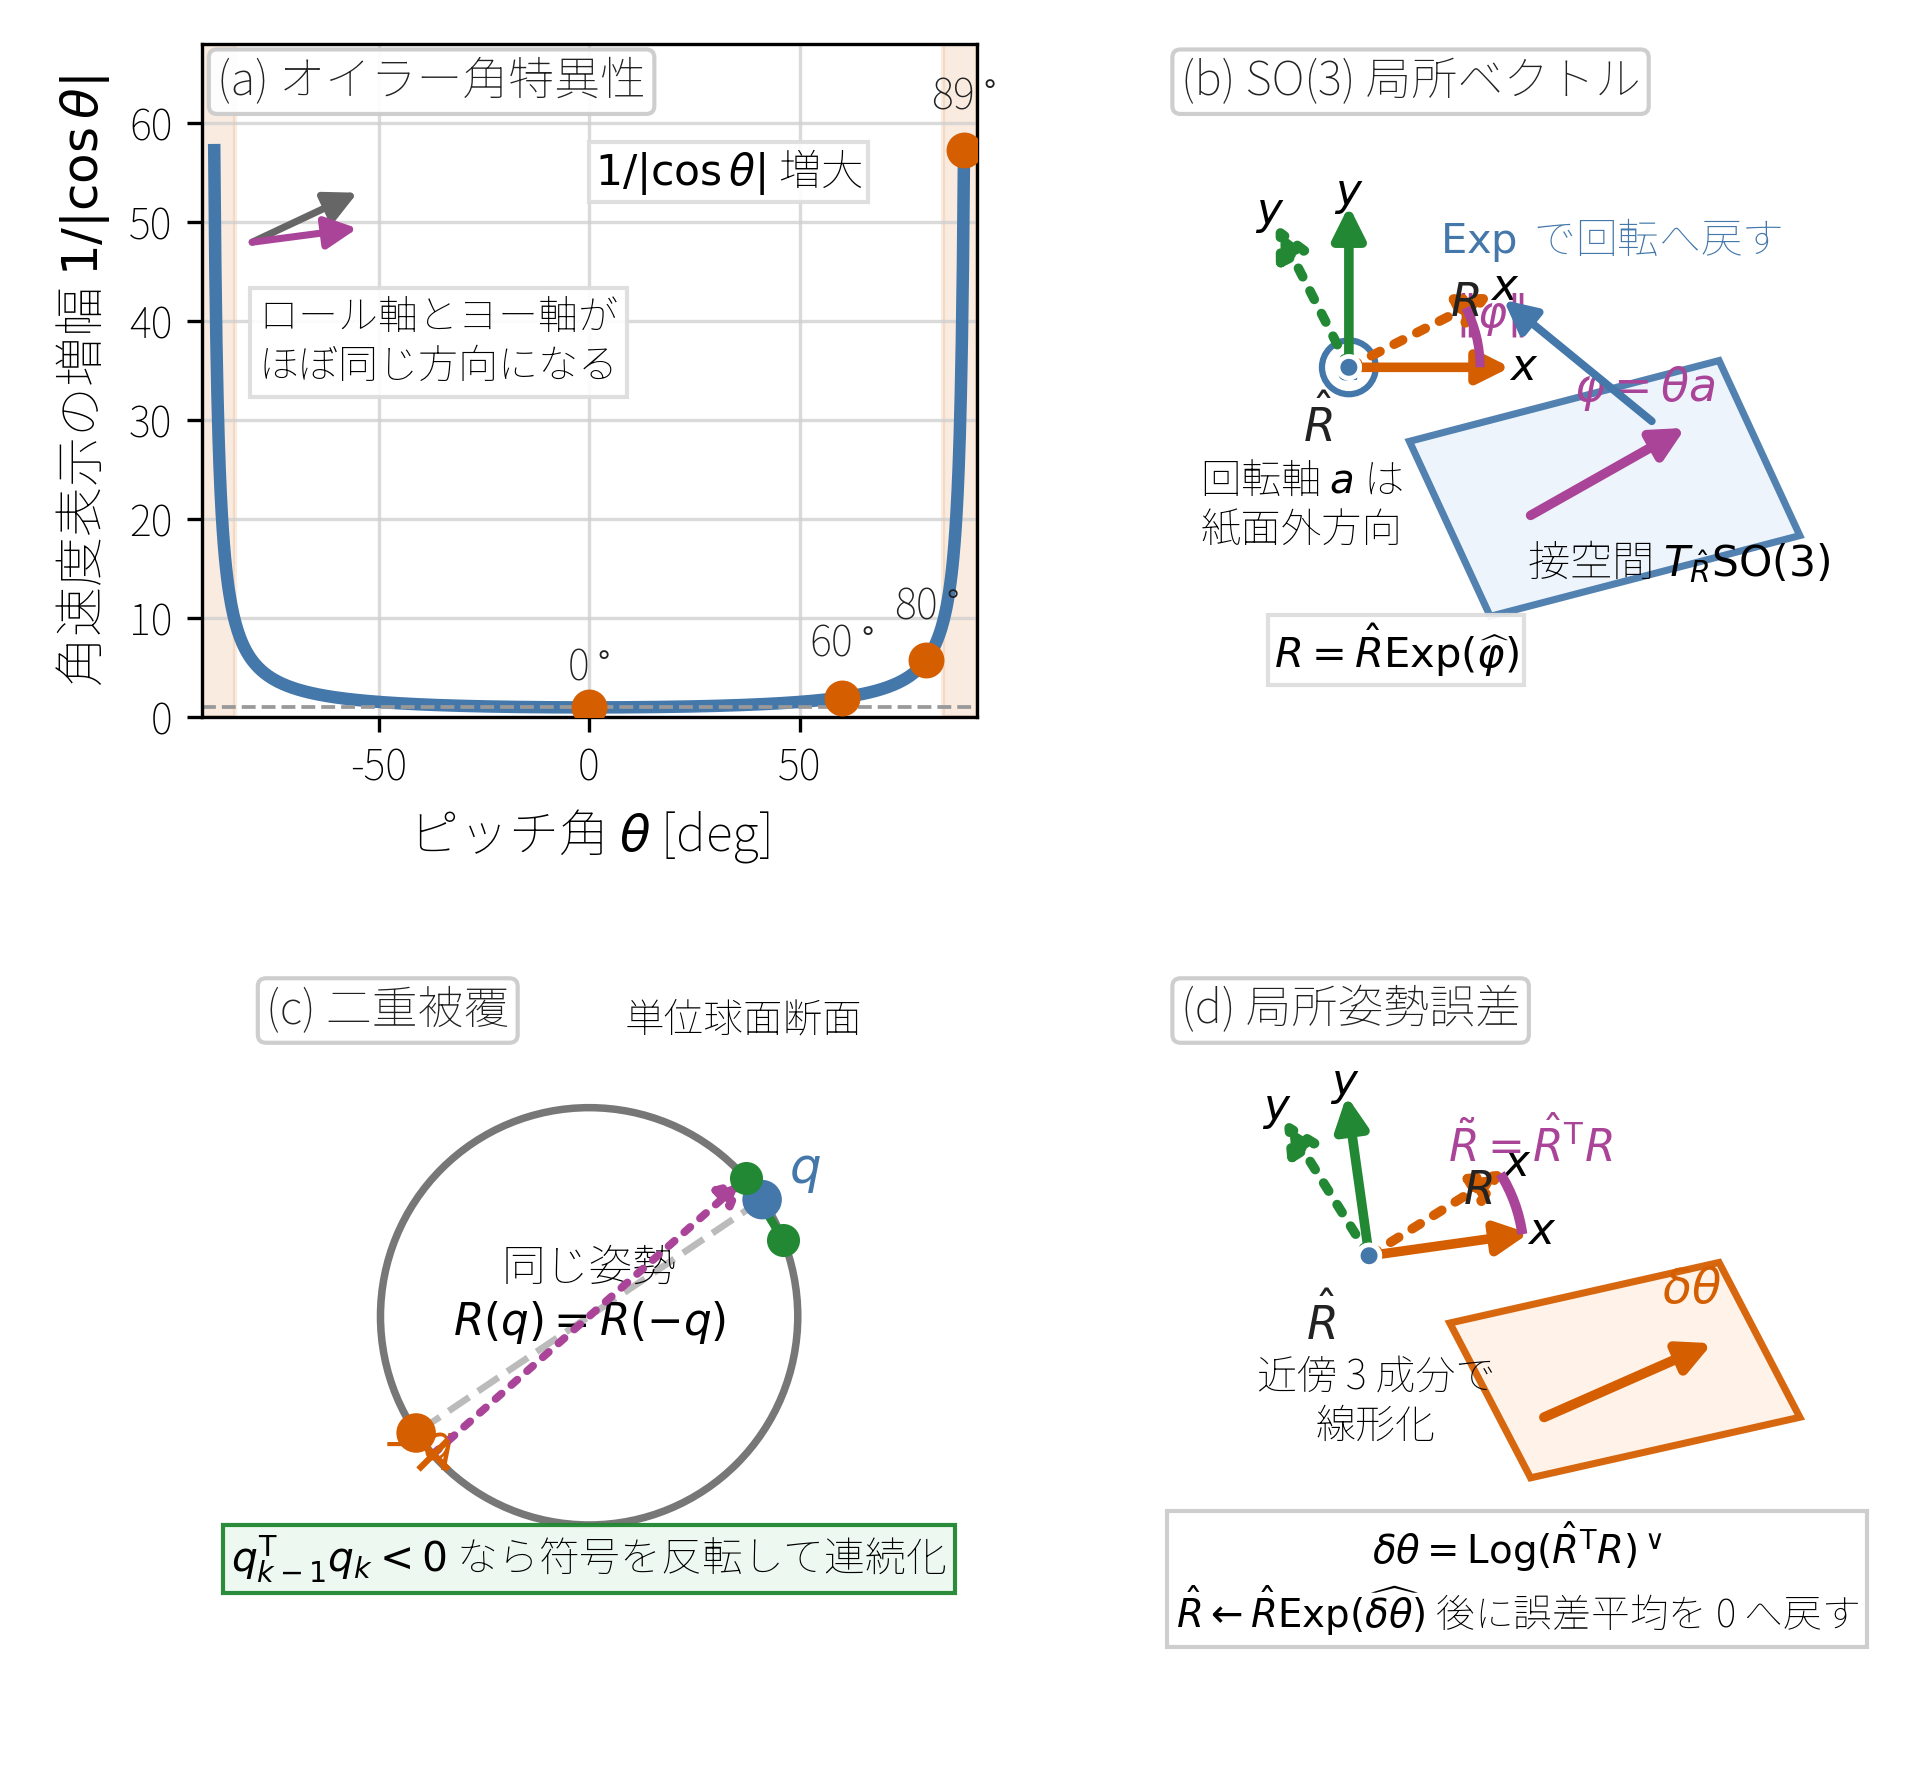
\includegraphics[width=\textwidth]{figures/flow6_attitude_geometry_examples.png}
\caption{三次元姿勢で同時に現れる幾何の要点。オイラー角はピッチ角が $\pm90^\circ$ に近づくと角速度表示が悪条件になり、$\SO(3)$ の指数写像と対数写像は名目姿勢の近くの小回転を接空間で扱う。単位四元数では $q$ と $-q$ が同じ姿勢を表すため、時系列では符号連続性を保つ。ESKF と姿勢制御では、相対回転から局所誤差 $\delta\theta$ を取り出して名目姿勢へ注入する。}
\label{fig:flow-six-attitude-geometry-examples}
\end{figure}

図\ref{fig:flow-six-attitude-geometry-examples}は、この節で導いた式を実装時の判断へ結びつける。左上の曲線は、ZYX オイラー角の逆変換に現れる $1/|\cos\theta|$ をピッチ角で変化させたものである。$\theta=0^\circ$ では機体系角速度 $r=0.10$ [rad/s] がヨー角速度 $\dot{\psi}=0.10$ [rad/s] として表れるが、$\theta=89^\circ$ では同じ実角速度が約 $5.73$ [rad/s] の表示になる。これは剛体が急に速く回ったという意味ではなく、ロール軸とヨー軸が表示上ほぼ同じ方向になり、角度座標が小さな回転を大きな角速度成分へ写すという意味である。

右上の図は、姿勢そのものを $\SO(3)$ 上の点として保ち、小さな回転だけを接空間のベクトル $\varphi$ として扱う見方を表している。$\operatorname{Exp}(\widehat{\varphi})$ は接空間の局所ベクトルを回転へ戻し、$\operatorname{Log}(R)^\vee$ は名目姿勢の近くの相対回転を三次元ベクトルへ戻す。このため、姿勢推定や NMPC の線形化では、全姿勢を一つのオイラー角座標で覆うのではなく、現在の名目姿勢を基準にして「近くの差」だけを線形モデルへ渡す。

左下の四元数の図は、単位四元数の符号が姿勢の符号ではないことを示している。$q$ と $-q$ は同じ回転を表すので、ログ上で符号が飛んでも実姿勢が $180^\circ$ 回ったとは限らない。連続した推定列や補間では、隣り合う四元数の内積が負になったときに片方の符号を反転し、同じ姿勢を近い点として扱う。この処理を入れないと、滑らかな姿勢変化を不連続な誤差として対数写像や補間へ渡してしまう。

右下の図は、ESKF と局所姿勢制御で使う誤差の作り方をまとめている。行列成分を直接引くのではなく、相対回転
\begin{equation}
  \tilde{R}=\hat{R}^\T R
\end{equation}
を作り、
\begin{equation}
  \delta\theta=\operatorname{Log}(\tilde{R})^\vee
\end{equation}
として [rad] 単位の三次元ベクトルを得る。小さい誤差であれば、この $\delta\theta$ は共分散、Kalman ゲイン、フィードバックトルクに入れられる局所座標である。更新後は $\hat{R}\leftarrow\hat{R}\operatorname{Exp}(\widehat{\delta\theta})$ のように名目姿勢へ注入し、誤差平均を 0 に戻す。したがって実装上の帰結は明確である。表示や仕様にはオイラー角を使ってよいが、積分、推定、フィードバック、制約評価では四元数または回転行列で姿勢を保ち、補正量だけを局所ベクトルとして扱う。

姿勢制御でも同じ構造を使う。目標姿勢を $R_d$、現在姿勢を $R$ とすれば
\begin{equation}
  e_R=\operatorname{Log}(R_d^\T R)^\vee
\end{equation}
は、目標姿勢から現在姿勢への局所的な姿勢誤差を [rad] 単位の三次元ベクトルとして与える。角速度誤差 $e_\omega=\omega-\omega_d$ と合わせて
\begin{equation}
  \tau=-K_Re_R-K_\omega e_\omega
\end{equation}
のような局所姿勢制御則を構成できる。ただし、これは小角度誤差を前提とする局所制御則であり、$\pi$ [rad] 近傍の姿勢差、入力飽和、慣性テンソルの不確かさを含む場合は、安定領域と制約を別に評価しなければならない。

以上の理由から、オイラー角、四元数、指数写像、対数写像は競合する表現ではなく、用途の異なる表現である。オイラー角は表示と仕様の記述に適し、四元数は特異点のない姿勢積分と合成に適し、指数写像と対数写像は小さな誤差、共分散、フィードバック誤差を三次元ベクトルとして扱うために適している。姿勢を含む非線形推定、NMPC、剛体姿勢制御では、これらを区別して使うことが、座標特異点と単位制約を破らない実装につながる。

\subsection{ニュートン・オイラー法}

ニュートン・オイラー法は、運動量と角運動量の収支から運動方程式を作る方法である。力が質点の並進運動を変え、モーメントが剛体の回転運動を変える、という二つの事実を同じ座標規約のもとで書く。制御でこの方法を使うときに重要なのは、公式の形そのものよりも、力、モーメント、速度、角速度をどの座標系の成分で表しているかをそろえることである。

\subsubsection{質点の運動量方程式}

質量 $m>0$ [kg] の質点を考える。慣性座標系 $\{I\}$ で表した位置を $p^I$ [m]、速度を
\begin{equation}
  v^I=\dot{p}^I
\end{equation}
とする。質量が時間で変わらず、相対論的な速度ではなく、$\{I\}$ が十分よい慣性系として扱えると仮定すれば、線形運動量は
\begin{equation}
  \ell^I=mv^I
\end{equation}
である。ニュートンの第二法則は
\begin{equation}
  \dot{\ell}^I=F^I
\end{equation}
なので、質量一定では
\begin{equation}
  m\dot{v}^I=F^I,\qquad
  \dot{p}^I=v^I
\end{equation}
となる。ここで $F^I$ [N] は慣性座標系成分で表した合力であり、$1\,\mathrm{N}=1\,\mathrm{kg\,m/s^2}$ である。

重力加速度を $g^I$ [m/s$^2$]、重力以外の外力を $f^I$ [N] と分けるなら
\begin{equation}
  m\dot{v}^I=mg^I+f^I
\end{equation}
である。外力が物体固定座標系 $\{B\}$ の成分 $f^B$ として与えられるなら、前節の座標変換を使って
\begin{equation}
  f^I=R^I_B f^B
\end{equation}
と変換してから並進方程式へ入れる。$m\dot{v}^I=mg^I+f^B$ と書くと、慣性座標系の加速度と物体固定座標系の力を混ぜることになり、次元は合っていても座標成分としては誤りである。

\subsubsection{重心並進と剛体の仮定}

剛体は、質点の集まりの相対位置が変わらない理想化である。剛体全体の並進運動は重心で代表させる。重心位置を $p^I$、重心速度を $v^I$ とすれば、重心に関する並進方程式は質点と同じ形で
\begin{equation}
  m\dot{v}^I=F^I
\end{equation}
である。ただし $F^I$ は剛体に作用するすべての外力の合力であり、重心まわりの内力は打ち消し合うと仮定している。

この単純な形は、原点を重心に置いていることに依存する。重心以外の点まわりに角運動量や運動エネルギーを書くと、並進速度と角速度の交差項が現れる。以下では、まず重心 $C$ に固定した物体固定座標系 $\{B\}$ を使い、質量分布が剛体内で変化せず、$\{B\}$ が剛体と一緒に回ると仮定する。

\subsubsection{慣性テンソル、角運動量、回転エネルギー}

剛体の回転しにくさは、質量だけでは決まらない。重心から遠い場所に質量があるほど、同じ角加速度を作るために大きなモーメントが必要になる。重心から微小質量要素への位置を
\begin{equation}
  r^B=
  \begin{bmatrix}
    x&y&z
  \end{bmatrix}^\T
\end{equation}
とし、単位行列を $I_3$ と書く。角速度を $\omega^B$ [rad/s] とすると、重心に対する微小質量要素の相対速度は $\omega^B\times r^B$ である。したがって、重心まわり角運動量の微小成分は
\begin{equation}
  \dd h_C^B
  =
  r^B\times\left((\omega^B\times r^B)\,\dd m\right)
\end{equation}
である。ベクトル三重積
\begin{equation}
  r\times(\omega\times r)
  =
  \left((r^\T r)I_3-rr^\T\right)\omega
\end{equation}
を用いると、剛体全体の角運動量は
\begin{align}
  h_C^B
  &=
  \int_{\mathcal{B}}
    r^B\times(\omega^B\times r^B)\,\dd m\\
  &=
  \left[
  \int_{\mathcal{B}}
    \left((r^B)^\T r^B\,I_3-r^B(r^B)^\T\right)\,\dd m
  \right]\omega^B
\end{align}
となる。ここで
\begin{equation}
  J_C^B
  =
  \int_{\mathcal{B}}
    \left((r^B)^\T r^B\,I_3-r^B(r^B)^\T\right)\,\dd m
\end{equation}
を重心まわり慣性テンソルという。慣性テンソルを一般記号 $I$ で書けば、角運動量と角速度の関係は
\begin{equation}
  h=I\omega
\end{equation}
であり、本節の座標付き記号では
\begin{equation}
  h_C^B=J_C^B\omega^B
\end{equation}
である。$J_C^B$ の単位は [kg\,m$^2$]、$h_C^B$ の単位は [kg\,m$^2$/s]、モーメント $\tau^B$ の単位は [N\,m]$=$[kg\,m$^2$/s$^2$] である。rad は無次元として扱うため、$\omega^B$ の次元は $1/\mathrm{s}$ である。

成分表示を使うと、慣性テンソルは
\begin{equation}
  J_C^B=
  \begin{bmatrix}
    \displaystyle\int(y^2+z^2)\,\dd m&
    \displaystyle-\int xy\,\dd m&
    \displaystyle-\int xz\,\dd m\\[1.0ex]
    \displaystyle-\int xy\,\dd m&
    \displaystyle\int(x^2+z^2)\,\dd m&
    \displaystyle-\int yz\,\dd m\\[1.0ex]
    \displaystyle-\int xz\,\dd m&
    \displaystyle-\int yz\,\dd m&
    \displaystyle\int(x^2+y^2)\,\dd m
  \end{bmatrix}
\end{equation}
である。対角成分は各軸まわりの慣性モーメントであり、非対角成分に現れる
\begin{equation}
  P_{xy}=\int xy\,\dd m,\qquad
  P_{xz}=\int xz\,\dd m,\qquad
  P_{yz}=\int yz\,\dd m
\end{equation}
を慣性乗積という。ここでは慣性乗積を正の積分量として定義したので、慣性テンソルの非対角成分は $-P_{xy}$、$-P_{xz}$、$-P_{yz}$ になる。慣性乗積は、選んだ座標軸に対して質量分布が斜めに偏っていることを表す。対称面が座標平面と一致すれば対応する慣性乗積は 0 になり、角速度の各成分と角運動量の各成分が混ざりにくくなる。

$J_C^B$ は実対称行列である。質量が一つの直線上だけに集中する退化的な場合を除けば正定値であり、任意の $\omega^B\ne0$ に対して
\begin{equation}
  (\omega^B)^\T J_C^B\omega^B>0
\end{equation}
を満たす。実対称行列のスペクトル分解により、直交行列 $Q$ を選んで
\begin{equation}
  Q^\T J_C^B Q
  =
  \operatorname{diag}(J_1,J_2,J_3)
\end{equation}
と対角化できる。$Q$ の列ベクトルは慣性主軸、$J_1,J_2,J_3$ は主慣性モーメントである。物体固定座標系を主軸に合わせれば慣性乗積は 0 になり、
\begin{equation}
  h_i=J_i\omega_i,\qquad i=1,2,3
\end{equation}
と成分ごとに読める。ただし、二つの主慣性モーメントが等しい場合、その二次元部分空間内の主軸の取り方は一意でない。

同じ定義から回転運動エネルギーも得られる。重心まわりの回転だけを見れば
\begin{align}
  T_\mathrm{rot}
  &=
  \frac{1}{2}
  \int_{\mathcal{B}}
    \norm{\omega^B\times r^B}^2\,\dd m\\
  &=
  \frac{1}{2}(\omega^B)^\T J_C^B\omega^B\\
  &=
  \frac{1}{2}(\omega^B)^\T h_C^B
\end{align}
である。単位は [J]$=$[kg\,m$^2$/s$^2$] である。重心の並進速度を $v_C^I$ とすれば、剛体全体の運動エネルギーは
\begin{equation}
  T=
  \frac{1}{2}m\norm{v_C^I}^2
  +
  \frac{1}{2}(\omega^B)^\T J_C^B\omega^B
\end{equation}
となる。重心を原点に取ったため、並進と回転の交差項は現れない。

慣性テンソルを重心以外の点 $O$ まわりで使いたい場合は、平行軸の定理を用いる。重心 $C$ から点 $O$ へのベクトルを $d^B$ [m] とし、座標軸の向きは変えないとする。このとき
\begin{equation}
  J_O^B
  =
  J_C^B
  +
  m\left((d^B)^\T d^B\,I_3-d^B(d^B)^\T\right)
\end{equation}
である。点 $O$ が重心から離れるほど、その点まわりの慣性テンソルは大きくなる。これは、同じ角速度でも質量中心が点 $O$ のまわりを並進するためである。

物体固定座標系 $\{B\}$ が剛体に固定されていれば、$J_C^B$ は時間で変わらない。以後、重心まわりであることが明らかなときは $J_C^B$ を $J^B$ と略記する。慣性座標系で見た角運動量の時間微分は外モーメントに等しいので、
\begin{equation}
  \left(\frac{\dd h}{\dd t}\right)^I=\tau^I
\end{equation}
である。これを回転する $\{B\}$ 成分で表すと、輸送定理により
\begin{equation}
  \left(\frac{\dd h}{\dd t}\right)^B
  =\dot{h}^B+\omega^B\times h^B
\end{equation}
となる。したがって、外モーメントを $\{B\}$ 成分 $\tau^B$ [N\,m] で表せば
\begin{align}
  \tau^B
  &=\dot{h}^B+\omega^B\times h^B\\
  &=J^B\dot{\omega}^B+\omega^B\times J^B\omega^B
\end{align}
を得る。これが物体固定座標系で書いた剛体回転のオイラー方程式である。第二項 $\omega^B\times J^B\omega^B$ は、回転する座標系で角運動量ベクトルの向きが変わることから現れる。$J^B$ が単位行列の定数倍である球対称剛体なら、この項は $\omega^B\times c\omega^B=0$ となるが、一般の剛体では角速度と角運動量が平行とは限らない。

主軸座標で $J^B=\operatorname{diag}(J_1,J_2,J_3)$ と書ける場合、オイラー方程式は
\begin{align}
  J_1\dot{\omega}_1+(J_3-J_2)\omega_2\omega_3&=\tau_1,\\
  J_2\dot{\omega}_2+(J_1-J_3)\omega_3\omega_1&=\tau_2,\\
  J_3\dot{\omega}_3+(J_2-J_1)\omega_1\omega_2&=\tau_3
\end{align}
となる。主軸を使うと慣性テンソルは対角化されるが、角速度成分の積による結合は残る。この結合が、姿勢制御、ジャイロ効果、回転体の安定性解析で重要になる。

\begin{example}[主軸からずれた座標系での角運動量と回転エネルギー]
重心まわりの主軸座標系 $\{P\}$ で
\begin{equation}
  J^P=\operatorname{diag}(0.02,\ 0.08,\ 0.10)\ \mathrm{kg\,m^2}
\end{equation}
である剛体を考える。物体固定座標系 $\{B\}$ の $x$ 軸と $y$ 軸が、主軸から $45^\circ$ 回転しているとする。このとき $\{B\}$ 成分の慣性テンソルは
\begin{equation}
  J^B=
  \begin{bmatrix}
    0.05&-0.03&0\\
    -0.03&0.05&0\\
    0&0&0.10
  \end{bmatrix}
  \ \mathrm{kg\,m^2}
\end{equation}
であり、$xy$ 慣性乗積は $P_{xy}=0.03$ [kg\,m$^2$] である。角速度が
\begin{equation}
  \omega^B=
  \begin{bmatrix}
    10\\0\\0
  \end{bmatrix}
  \ \mathrm{rad/s}
\end{equation}
なら、角運動量は
\begin{equation}
  h^B=J^B\omega^B
  =
  \begin{bmatrix}
    0.50\\-0.30\\0
  \end{bmatrix}
  \ \mathrm{kg\,m^2/s}
\end{equation}
である。角速度は $\{B\}$ の $x$ 軸方向だけを向いているが、角運動量には $y$ 成分が現れる。これは、$\{B\}$ の $x$ 軸が慣性主軸でないためである。

同じ瞬間の回転運動エネルギーは
\begin{equation}
  T_\mathrm{rot}
  =
  \frac{1}{2}(\omega^B)^\T J^B\omega^B
  =
  \frac{1}{2}\cdot 10\cdot0.50
  =
  2.5\ \mathrm{J}
\end{equation}
である。主軸に沿って座標を取り直せば慣性テンソルは対角行列に戻り、同じ物理量を混合成分なしで表せる。したがって、慣性乗積は剛体そのものだけでなく、選んだ座標軸にも依存する量である。
\end{example}

\subsubsection{座標系を明示した6自由度状態方程式}

空間剛体の 6 自由度とは、三つの並進自由度と三つの姿勢自由度を合わせた自由度数である。状態ベクトルの成分数が 6 という意味ではない。速度と角速度も状態に含めるので、回転行列で姿勢を表すなら
\begin{equation}
  x=\left(p^I,\ v^I,\ R^I_B,\ \omega^B\right)
\end{equation}
を状態として扱う。四元数を使う実装では
\begin{equation}
  x=
  \begin{bmatrix}
    (p^I)^\T&(v^I)^\T&(q^I_B)^\T&(\omega^B)^\T
  \end{bmatrix}^\T,
  \qquad
  \norm{q^I_B}=1
\end{equation}
のように書く。これは数値上は 13 成分を持つが、四元数には単位制約があるため、姿勢の独立自由度は 3 である。

重力以外の合力を物体固定座標系成分 $f^B$ [N]、重心まわり合モーメントを $\tau^B$ [N\,m] とする。重力加速度 $g^I$ [m/s$^2$] を含めた 6 自由度剛体モデルは
\begin{align}
  \dot{p}^I&=v^I,\\
  m\dot{v}^I&=mg^I+R^I_B f^B,\\
  \dot{R}^I_B&=R^I_B[\omega^B]_\times,\\
  J^B\dot{\omega}^B+\omega^B\times J^B\omega^B&=\tau^B
  \label{eq:euler-rigid}
\end{align}
である。第一式と第二式は慣性座標系での位置と速度の運動、第三式と第四式は物体固定座標系角速度を使った姿勢と回転運動である。$R^I_B f^B$ は、物体固定座標系で作られた合力を慣性座標系へ変換している。一方、回転方程式は $J^B$ が定数として使えるように物体固定座標系で書いている。このように、並進は $\{I\}$、回転は $\{B\}$ で書く混合表現がよく使われるが、各項の成分表示は必ず式ごとに一致させる。

入力 $u$ がそのまま力やモーメントであるとは限らない。アクチュエータの推力、接触力、ばね力、空気抵抗、拘束反力などを合成して $f^B(u,x,t)$ と $\tau^B(u,x,t)$ が作られる。したがって 6 自由度モデルは
\begin{equation}
  \dot{x}=f_\mathrm{6dof}(x,u,t)
\end{equation}
という非線形状態方程式であり、姿勢による座標変換、角速度の積、入力から力・モーメントへの写像が非線形性の主な発生源になる。

\subsubsection{力とモーメントの入力写像}

複数の外力が作用する場合、各作用点の重心からの位置を $r_i^B$ [m]、その点での力を $f_i^B$ [N]、力以外に直接加わるモーメントを $\tau_i^B$ [N\,m] とする。重心まわりの合力と合モーメントは
\begin{align}
  f^B&=\sum_{i=1}^{N_f} f_i^B,\\
  \tau^B&=\sum_{i=1}^{N_f} r_i^B\times f_i^B
          +\sum_{i=1}^{N_\tau}\tau_i^B
\end{align}
である。力の作用線が重心を通れば $r_i^B\times f_i^B=0$ であり、その力は重心まわりの回転を直接は作らない。反対に、同じ力でも作用点が重心から離れていればモーメントを生む。推力の大きさや向きが入力で変わる場合、$u\mapsto(f^B,\tau^B)$ は一般に非線形写像になる。後で扱う制御配分は、この写像を使って、望ましい合力・合モーメントを複数アクチュエータの入力へ分配する問題である。

\subsubsection{再帰的 Newton-Euler 法の解釈}

多関節機構では、各リンクについて同じ運動量収支を一つずつ書くと式が長くなる。再帰的 Newton-Euler 法は、リンク列に沿って二つの計算を行う。外向き計算では、根元から先端へ角速度、角加速度、重心加速度を伝搬する。内向き計算では、先端から根元へ力とモーメントを戻し、各関節が負担すべき一般化力やトルクを求める。

この方法は、6 自由度剛体方程式と別の物理法則ではない。各リンクに対して
\begin{equation}
  F=m a,\qquad
  \tau=J\dot{\omega}+\omega\times J\omega
\end{equation}
を座標変換と作用反作用を保ちながら順に適用している。したがって、単一剛体の 6 自由度モデルを理解しておくと、多リンク機構の再帰計算も、速度・加速度を前へ送り、力・モーメントを後ろへ戻す整理として解釈できる。

\begin{example}[偏心した力を受ける剛体の瞬間加速度]
質量 $m=2$ [kg] の剛体を考える。姿勢は水平面内のヨー角 $\psi=\pi/6$ [rad] だけ回転しており、$R^I_B=R_z(\psi)$ とする。物体固定座標系で、重心から
\begin{equation}
  r^B=
  \begin{bmatrix}0\\0.2\\0\end{bmatrix}\ \mathrm{m}
\end{equation}
の位置に
\begin{equation}
  f^B=
  \begin{bmatrix}4\\0\\0\end{bmatrix}\ \mathrm{N}
\end{equation}
の力が作用する。ここでは重力は別途つり合っているか、水平面内の運動だけを見ているとして、$g^I=0$ とおく。

慣性座標系で見た合力は
\begin{equation}
  f^I=R_z(\pi/6)f^B
  =
  \begin{bmatrix}
    2\sqrt{3}\\2\\0
  \end{bmatrix}\ \mathrm{N}
\end{equation}
である。したがって重心加速度は
\begin{equation}
  \dot{v}^I=\frac{1}{m}f^I
  =
  \begin{bmatrix}
    \sqrt{3}\\1\\0
  \end{bmatrix}\ \mathrm{m/s^2}
\end{equation}
となる。同じ力を $f^B=[4\ 0\ 0]^\T$ のまま $\dot{v}^I$ に代入すると、物体の向きによる加速度方向の変化を失う。

重心まわりのモーメントは
\begin{equation}
  \tau^B=r^B\times f^B
  =
  \begin{bmatrix}0\\0.2\\0\end{bmatrix}
  \times
  \begin{bmatrix}4\\0\\0\end{bmatrix}
  =
  \begin{bmatrix}0\\0\\-0.8\end{bmatrix}\ \mathrm{N\,m}
\end{equation}
である。慣性テンソルを
\begin{equation}
  J^B=\operatorname{diag}(0.1,\ 0.2,\ 0.3)\ \mathrm{kg\,m^2}
\end{equation}
とし、その瞬間の角速度が $\omega^B=0$ なら、ジャイロ項は 0 なので
\begin{equation}
  \dot{\omega}^B=(J^B)^{-1}\tau^B
  =
  \begin{bmatrix}
    0\\0\\-0.8/0.3
  \end{bmatrix}\ \mathrm{rad/s^2}
\end{equation}
である。この計算から、同じ外力が並進加速度と回転加速度の両方を作り、並進では座標変換 $R^I_B$、回転では作用点の腕 $r^B$ と慣性テンソル $J^B$ が必要になることが分かる。
\end{example}

\subsection{オイラー・ラグランジュ法}

ニュートン・オイラー法は、力とモーメントを座標軸に分解し、運動量と角運動量の収支から式を作る方法であった。これに対して、拘束の多い機械では、拘束を満たす座標を先に選び、エネルギーと仮想仕事から運動方程式を作る方が短くなることが多い。オイラー・ラグランジュ法は、この目的のための標準的な定式化である。

まず、質点や剛体上の代表点の位置をまとめて $r_1,\ldots,r_N$ とする。各 $r_j$ は三次元なら $\R^3$ のベクトルであり、単位は [m] である。すべての位置成分をそのまま座標にすると自由度は大きいが、棒の長さ、レール、関節、回転軸のような幾何拘束があると、実際に独立に動ける方向は少なくなる。たとえば平面内の単振子では、質点の位置 $(x,y)$ は
\begin{equation}
  x^2+y^2=l^2
\end{equation}
を満たすため、二つの座標 $(x,y)$ を独立には選べない。この拘束を角度 $\theta$ で解けば
\begin{equation}
  x=l\sin\theta,\qquad
  y=-l\cos\theta
\end{equation}
となり、必要な座標は一つになる。このように、拘束を満たす運動を
\begin{equation}
  r_j=r_j(q,t),\qquad
  q=
  \begin{bmatrix}
    q_1&\cdots&q_n
  \end{bmatrix}^\T
\end{equation}
と表すとき、$q\in\R^n$ を一般化座標という。$q_i$ の単位は、長さ [m]、角度 [rad]、無次元量など、選んだ座標に依存する。対応する時間微分 $\dot{q}$ を一般化速度という。ここでは、拘束が位置と時間の関係として表され、上のように $q$ で解ける場合を考える。拘束を明示的に解けない場合や接触反力を知りたい場合は、ラグランジュ未定乗数を使う定式化が必要になる。

仮想変位は、時刻 $t$ を固定したまま、拘束を破らない範囲で位置を少しだけ動かす変位である。$q_i$ を $\delta q_i$ だけ変えると、代表点の仮想変位は
\begin{equation}
  \delta r_j
  =
  \sum_{i=1}^n
  \frac{\pp r_j}{\pp q_i}\delta q_i
\end{equation}
である。実際の時間変化 $\dd r_j$ ではなく、同じ時刻における許される方向だけを見る点が重要である。力 $F_j$ [N] が代表点 $r_j$ に作用すると、仮想仕事は
\begin{align}
  \delta W
  &=
  \sum_{j=1}^N F_j^\T\delta r_j\\
  &=
  \sum_{j=1}^N
  F_j^\T
  \left(
    \sum_{i=1}^n
    \frac{\pp r_j}{\pp q_i}\delta q_i
  \right)\\
  &=
  \sum_{i=1}^n
  \left(
    \sum_{j=1}^N
    F_j^\T\frac{\pp r_j}{\pp q_i}
  \right)\delta q_i
\end{align}
となる。この係数
\begin{equation}
  Q_i=
  \sum_{j=1}^N
  F_j^\T\frac{\pp r_j}{\pp q_i}
\end{equation}
を $q_i$ に対応する一般化力という。$q_i$ が長さなら $Q_i$ の単位は [N]、$q_i$ が角度なら $Q_i$ の単位は [N\,m] であり、$Q_i\delta q_i$ が仕事 [J] になるように決まる。理想的な拘束反力は、許される仮想変位に対して仕事をしないため、一般化力の式から消える。これが、拘束反力を一つずつ解かずに運動方程式を作れる理由である。

運動エネルギーは、質点であれば
\begin{equation}
  T(q,\dot{q},t)
  =
  \frac{1}{2}
  \sum_{j=1}^N
  m_j\dot{r}_j^\T\dot{r}_j
\end{equation}
である。剛体を含む場合は、各剛体について並進の運動エネルギーに加えて、前に導入した角速度と慣性テンソルによる回転エネルギー
\begin{equation}
  \frac{1}{2}\omega^\T J\omega
\end{equation}
を足せばよい。重力やばねのようにポテンシャルエネルギーで表せる保存力については
\begin{equation}
  V=V(q,t)
\end{equation}
を定める。ラグランジアンを
\begin{equation}
  L(q,\dot{q},t)=T(q,\dot{q},t)-V(q,t)
\end{equation}
と定義する。

\begin{derivation}
拘束を満たす仮想変位に対して、ダランベールの原理は
\begin{equation}
  \sum_{j=1}^N
  \left(F_j-m_j\ddot{r}_j\right)^\T\delta r_j=0
\end{equation}
と書ける。これは、力 $F_j$ に慣性力 $-m_j\ddot{r}_j$ を加えると、許される仮想変位に対する仮想仕事が 0 になる、という形でニュートンの運動方程式を書き直したものである。仮想変位の式を代入すると、任意の $\delta q_i$ に対して
\begin{equation}
  \sum_{j=1}^N
  F_j^\T\frac{\pp r_j}{\pp q_i}
  -
  \sum_{j=1}^N
  m_j\ddot{r}_j^\T\frac{\pp r_j}{\pp q_i}
  =0
\end{equation}
が成り立つ。

ここで、運動エネルギーから生じる恒等式を確認する。$r_j=r_j(q,t)$ であるから
\begin{equation}
  \frac{\pp \dot{r}_j}{\pp \dot{q}_i}
  =
  \frac{\pp r_j}{\pp q_i}
\end{equation}
である。したがって
\begin{equation}
  \frac{\pp T}{\pp \dot{q}_i}
  =
  \sum_{j=1}^N
  m_j\dot{r}_j^\T
  \frac{\pp r_j}{\pp q_i}
\end{equation}
となる。両辺を時間微分すると
\begin{equation}
  \frac{\dd}{\dd t}
  \frac{\pp T}{\pp \dot{q}_i}
  =
  \sum_{j=1}^N
  m_j\ddot{r}_j^\T
  \frac{\pp r_j}{\pp q_i}
  +
  \sum_{j=1}^N
  m_j\dot{r}_j^\T
  \frac{\dd}{\dd t}
  \left(
    \frac{\pp r_j}{\pp q_i}
  \right)
\end{equation}
である。一方、滑らかな座標変換では偏微分と時間微分が交換できるので
\begin{equation}
  \frac{\pp \dot{r}_j}{\pp q_i}
  =
  \frac{\dd}{\dd t}
  \left(
    \frac{\pp r_j}{\pp q_i}
  \right)
\end{equation}
であり、
\begin{equation}
  \frac{\pp T}{\pp q_i}
  =
  \sum_{j=1}^N
  m_j\dot{r}_j^\T
  \frac{\dd}{\dd t}
  \left(
    \frac{\pp r_j}{\pp q_i}
  \right)
\end{equation}
となる。よって
\begin{equation}
  \frac{\dd}{\dd t}
  \frac{\pp T}{\pp \dot{q}_i}
  -
  \frac{\pp T}{\pp q_i}
  =
  \sum_{j=1}^N
  m_j\ddot{r}_j^\T
  \frac{\pp r_j}{\pp q_i}
\end{equation}
が得られる。

保存力がポテンシャル $V(q,t)$ から来るとき、その一般化力は
\begin{equation}
  Q_i^\mathrm{c}=-\frac{\pp V}{\pp q_i}
\end{equation}
である。保存力以外の力、たとえば入力トルク、モータ力、粘性摩擦、空気抵抗をまとめて $Q_i^\mathrm{nc}$ と書くと
\begin{equation}
  \frac{\dd}{\dd t}
  \frac{\pp T}{\pp \dot{q}_i}
  -
  \frac{\pp T}{\pp q_i}
  =
  -\frac{\pp V}{\pp q_i}+Q_i^\mathrm{nc}
\end{equation}
である。$L=T-V$ かつ $V$ が $\dot{q}$ に依存しないことから
\begin{equation}
  \frac{\dd}{\dd t}
  \frac{\pp L}{\pp \dot{q}_i}
  -
  \frac{\pp L}{\pp q_i}
  =
  Q_i^\mathrm{nc},
  \qquad i=1,\ldots,n
\end{equation}
を得る。これがオイラー・ラグランジュ方程式である。
\end{derivation}

保存力だけが作用する自由運動では右辺は 0 になる。制御入力や摩擦がある制御対象では、右辺に一般化された非保存力を入れる。入力 $u\in\R^m$ が一般化座標へ行列 $B(q)$ を通じて作用するなら
\begin{equation}
  Q^\mathrm{nc}=B(q)u-D(q,\dot{q})
\end{equation}
のように書ける。ここで $D$ は粘性摩擦や抵抗を含む項である。機械系の多くは、整理すると
\begin{equation}
  M(q)\ddot{q}+c(q,\dot{q})+g(q)=Q^\mathrm{nc}
\end{equation}
の形になる。$M(q)$ は一般化座標で見た慣性行列、$c(q,\dot{q})$ は速度に依存する遠心力・コリオリ力・抵抗の項、$g(q)$ はポテンシャル勾配から来る項である。

\begin{example}[単振子の一般化座標による導出]
質量 $m>0$ [kg] の質点が長さ $l>0$ [m] の質量のない棒または糸で支えられ、鉛直下向きを $\theta=0$ とする。直交座標 $(x,y)$ を使うと拘束 $x^2+y^2=l^2$ があるが、一般化座標を角度 $\theta$ [rad] とすれば
\begin{equation}
  x=l\sin\theta,\qquad
  y=-l\cos\theta
\end{equation}
で拘束を自動的に満たす。速度は
\begin{equation}
  \dot{x}=l\cos\theta\,\dot{\theta},
  \qquad
  \dot{y}=l\sin\theta\,\dot{\theta}
\end{equation}
なので
\begin{equation}
  T=\frac{1}{2}ml^2\dot{\theta}^2,
  \qquad
  V=mgl(1-\cos\theta)
\end{equation}
である。したがって
\begin{equation}
  L
  =
  \frac{1}{2}ml^2\dot{\theta}^2
  -
  mgl(1-\cos\theta)
\end{equation}
となる。各項を計算すると
\begin{align}
  \frac{\pp L}{\pp\dot{\theta}}
  &=
  ml^2\dot{\theta},&
  \frac{\dd}{\dd t}
  \frac{\pp L}{\pp\dot{\theta}}
  &=
  ml^2\ddot{\theta},\\
  \frac{\pp L}{\pp\theta}
  &=
  -mgl\sin\theta
\end{align}
である。支点まわりの入力トルクを $\tau$ [N\,m]、粘性摩擦を $b\dot{\theta}$ [N\,m] とすれば、非保存一般化力は
\begin{equation}
  Q^\mathrm{nc}=\tau-b\dot{\theta}
\end{equation}
である。オイラー・ラグランジュ方程式より
\begin{equation}
  ml^2\ddot{\theta}+mgl\sin\theta=\tau-b\dot{\theta}
\end{equation}
を得る。小角近似で $\sin\theta\simeq\theta$ とすれば
\begin{equation}
  ml^2\ddot{\theta}+b\dot{\theta}+mgl\theta=\tau
\end{equation}
という線形二次系になる。一方、大きな角度では $\sin\theta$ の非線形性が残る。この例では、棒または糸の張力を未知の拘束反力として求めなくても、角度という一般化座標を選ぶだけで運動方程式を得られる。
\end{example}

\subsubsection{拘束ヤコビアンとラグランジュ未定乗数}

一般化座標を選ぶだけで拘束を消去できる場合でも、拘束反力そのものを知りたい、または接触が成立したり離れたりする状況を扱いたい場合には、拘束を式として残した方がよい。位置と時間だけで書ける等式拘束
\begin{equation}
  \phi(q,t)=0,\qquad
  \phi:\R^n\times\R\to\R^k
\end{equation}
をホロノミック拘束という。棒の長さ、レール上の運動、回転軸、平面接触が保たれている間の法線方向位置などは、典型的なホロノミック拘束である。拘束の一次感度
\begin{equation}
  J_c(q,t)=\frac{\pp \phi}{\pp q}(q,t)\in\R^{k\times n}
\end{equation}
を拘束ヤコビアンという。拘束を時間微分すると
\begin{equation}
  J_c(q,t)\dot{q}+\frac{\pp \phi}{\pp t}(q,t)=0
\end{equation}
となるため、許される速度は拘束ヤコビアンの零空間に制限される。時間に陽に依存しない拘束なら、式は単に $J_c(q)\dot{q}=0$ である。

一方、拘束が速度の関係として与えられ、一般には位置だけの等式へ積分できない場合を非ホロノミック拘束という。基本形は
\begin{equation}
  A_c(q,t)\dot{q}=b_c(q,t)
\end{equation}
である。車輪が横滑りしない条件のように、瞬間的に許される速度方向は制限されるが、位置だけで到達可能な集合を一つの面として表せない拘束がこれに当たる。非ホロノミック拘束は、座標を減らす通常のホロノミック拘束とは異なり、運動方程式と速度拘束を同時に解く問題として扱う。線形な速度拘束に対する工学的なラグランジュ・ダランベールの扱いでは、拘束力は $A_c(q,t)^\T\lambda$ の形で一般化力に現れる。

ホロノミック拘束に戻り、理想拘束を仮定する。理想拘束とは、拘束を破らない仮想変位 $\delta q$ に対して拘束反力が仕事をしない拘束である。許される仮想変位は
\begin{equation}
  J_c(q,t)\delta q=0
\end{equation}
を満たす。拘束反力の一般化力 $Q_c$ がすべての許される $\delta q$ に対して $Q_c^\T\delta q=0$ を満たすなら、$Q_c$ は $J_c$ の行空間に属する。したがって、ある $\lambda\in\R^k$ を用いて
\begin{equation}
  Q_c=J_c(q,t)^\T\lambda
\end{equation}
と書ける。この $\lambda$ をラグランジュ未定乗数という。未定乗数は単なる計算上の係数ではなく、拘束式の単位で測った拘束反力である。たとえば $\phi(q)=y$ が床からの高さ [m] を表すなら、$\lambda$ の単位は [N] であり、接触法線力そのものになる。$\phi(q)=x^2+y^2-l^2$ のように [m$^2$] の拘束を使うと、$\lambda$ の単位は変わるが、実際の一般化力 $J_c^\T\lambda$ は同じ物理量を表す。

拘束を残したオイラー・ラグランジュ方程式は
\begin{align}
  M(q)\ddot{q}+c(q,\dot{q})+g(q)
  &=Q^\mathrm{nc}+J_c(q,t)^\T\lambda,\\
  \phi(q,t)&=0
\end{align}
である。加速度レベルで拘束を満たすには、速度拘束をさらに微分して
\begin{equation}
  J_c(q,t)\ddot{q}
  +\dot{J}_c(q,t)\dot{q}
  +\frac{\dd}{\dd t}
    \left(\frac{\pp \phi}{\pp t}(q,t)\right)
  =0
\end{equation}
を課す。右辺をまとめて
\begin{equation}
  \gamma_c(q,\dot{q},t)
  =
  \dot{J}_c(q,t)\dot{q}
  +\frac{\dd}{\dd t}
    \left(\frac{\pp \phi}{\pp t}(q,t)\right)
\end{equation}
と書けば、$\ddot{q}$ と $\lambda$ は鞍点型の線形方程式
\begin{equation}
  \begin{bmatrix}
    M(q)&-J_c(q,t)^\T\\
    J_c(q,t)&0
  \end{bmatrix}
  \begin{bmatrix}
    \ddot{q}\\
    \lambda
  \end{bmatrix}
  =
  \begin{bmatrix}
    Q^\mathrm{nc}-c(q,\dot{q})-g(q)\\
    -\gamma_c(q,\dot{q},t)
  \end{bmatrix}
\end{equation}
から同時に求められる。この形は、拘束を満たす加速度と、その加速度を実現するために必要な拘束反力を同時に計算する式である。数値計算では $M(q)$ が正定値で、拘束ヤコビアンの行が独立であることが、未定乗数の一意性に関係する。

\subsubsection{片側接触とクーロン摩擦}

接触は、等式拘束だけでは表しきれない。床や壁は物体を押すことはできるが、引っ張ることはできないためである。接触候補点のすき間を
\begin{equation}
  \phi_n(q)\ge0
\end{equation}
と定義する。$\phi_n(q)>0$ なら物体は離れており、法線接触力は 0 である。$\phi_n(q)=0$ のときだけ、押し返す法線力 $\lambda_n\ge0$ が発生できる。この直感を相補性条件として書くと
\begin{equation}
  \phi_n(q)\ge0,\qquad
  \lambda_n\ge0,\qquad
  \lambda_n\phi_n(q)=0
\end{equation}
である。最後の式は、すき間が正なら法線力が 0 であり、法線力が正ならすき間が 0 であることを表す。接触が保たれている区間では、$J_n=\pp\phi_n/\pp q$ を法線方向の拘束ヤコビアンとして、法線接触力の一般化力は $J_n(q)^\T\lambda_n$ になる。

接触点に接線方向の相対速度 $v_t$ があると、摩擦力 $f_t$ が接線方向に働く。クーロン摩擦では、法線力を $\lambda_n$、摩擦係数を $\mu\ge0$ として
\begin{equation}
  \norm{f_t}\le\mu\lambda_n
\end{equation}
を満たす力の集合を摩擦円錐という。接触が滑っているとき、摩擦力は滑り速度と逆向きで、円錐の境界に乗る：
\begin{equation}
  f_t=-\mu\lambda_n\frac{v_t}{\norm{v_t}},
  \qquad v_t\ne0.
\end{equation}
接触が固着しているときは $v_t=0$ であり、摩擦力は一意には決まらない。必要な接線力が
\begin{equation}
  \norm{f_t}<\mu\lambda_n
\end{equation}
の内側に収まるなら固着を保てるが、必要な力が境界を超えると滑りへ移る。したがって静止摩擦は「大きさが常に $\mu\lambda_n$ の力」ではなく、固着を保つために円錐内で値が選ばれる拘束力である。

摩擦を含むモデルには、滑りと固着の切替、速度 0 での不連続、接触の発生と消失、衝突時の速度跳躍がある。滑らかな通常の状態方程式だけで全てを表すと、接触直前や停止直前で数値的に不安定になることがある。実装では、摩擦円錐を多面体で近似する、微小速度で正則化する、時間離散化した相補性問題として解く、衝突をインパルスとして別に扱う、といった選択が必要になる。制御設計で摩擦を「粘性抵抗」として単純化する場合も、低速での固着、最大静止摩擦、法線力の変化が無視されていることを明示しておく。

\begin{example}[水平床上の質点に働く法線力と摩擦]
質量 $m$ の質点が水平床の上を動く。座標を $q=[x\ y]^\T$ とし、$y$ 軸を上向き、床を $y=0$ とする。重力は $[0\ -mg]^\T$、水平方向の入力は $[u\ 0]^\T$ である。床とのすき間は
\begin{equation}
  \phi_n(q)=y\ge0,
  \qquad
  J_n=\frac{\pp \phi_n}{\pp q}
  =
  \begin{bmatrix}0&1\end{bmatrix}
\end{equation}
である。接触が保たれている間は $y=0$、$\dot{y}=0$、$\ddot{y}=0$ であり、運動方程式は
\begin{equation}
  m
  \begin{bmatrix}
    \ddot{x}\\
    \ddot{y}
  \end{bmatrix}
  =
  \begin{bmatrix}
    u+f_t\\
    -mg+\lambda_n
  \end{bmatrix}
\end{equation}
となる。鉛直方向の拘束加速度 $\ddot{y}=0$ から
\begin{equation}
  -mg+\lambda_n=0,
  \qquad
  \lambda_n=mg
\end{equation}
を得る。すなわち、この単純な状況では、未定乗数は床が質点を押し返す法線力であり、重力と釣り合う。

水平方向の相対速度は $v_t=\dot{x}$ である。滑っているときは
\begin{equation}
  f_t=-\mu mg\,\operatorname{sgn}(\dot{x}),
  \qquad
  \dot{x}\ne0
\end{equation}
であり、
\begin{equation}
  m\ddot{x}=u-\mu mg\,\operatorname{sgn}(\dot{x})
\end{equation}
となる。静止して固着している候補では $\dot{x}=0$、$\ddot{x}=0$ なので、水平式から $f_t=-u$ が必要である。これが摩擦円錐の一次元版
\begin{equation}
  \abs{f_t}\le\mu mg
\end{equation}
を満たす条件は
\begin{equation}
  \abs{u}\le\mu mg
\end{equation}
である。したがって、入力が最大静止摩擦以下なら質点は床に固着して動かず、入力がそれを超えると滑りが始まる。この例は、法線方向では片側拘束と未定乗数、接線方向では摩擦円錐と滑り・固着の切替が同時に現れる最小の接触モデルである。
\end{example}

ニュートン・オイラー法とオイラー・ラグランジュ法は競合する公式ではなく、同じ物理を別の座標で表す二つの方法である。拘束反力や接触力そのものを知りたい場合、または作用点ごとの力の流れを追いたい場合はニュートン・オイラー法が直接的である。独立自由度が少なく、エネルギーが簡潔に書ける場合は、オイラー・ラグランジュ法が運動方程式の導出を短くする。

\subsection{標準例による力学モデルの構成}

力学モデルを制御へ使うときは、座標を選び、状態を決め、力またはエネルギーから運動方程式を作り、入力と出力を明示する。この手順は、対象が質点でも、多リンク機構でも同じである。以下では、同じ記号の流れで四つの標準例を整理する。各例で得られる式は、シミュレーション、線形化、状態推定、フィードバック設計に渡すための非線形状態方程式である。

\subsubsection{力入力を受ける質点}

質量 $m>0$ [kg] の質点が $r$ 次元空間を動くとする。位置を $q\in\R^r$ [m]、速度を $v=\dot{q}$ [m/s] とし、状態を
\begin{equation}
  x=
  \begin{bmatrix}
    q^\T&v^\T
  \end{bmatrix}^\T
\end{equation}
に選ぶ。質点は大きさを持たず、回転エネルギー、姿勢、変形を無視できると仮定する。保存力がポテンシャル $V(q)$ [J] から生じ、粘性抵抗を $D v$、入力力を $u\in\R^r$ [N]、外乱力を $d$ [N] とすれば、
\begin{equation}
  T=\frac{1}{2}m v^\T v,
  \qquad
  F=-\nabla V(q)-Dv+u+d
\end{equation}
である。ニュートンの第二法則より
\begin{align}
  \dot{q}&=v,\\
  m\dot{v}&=-\nabla V(q)-Dv+u+d
\end{align}
を得る。出力は、位置制御なら $y=q$、速度も測るなら $y=[q^\T\ v^\T]^\T$ と置く。$V(q)=0$、$D=0$、$d=0$ なら
\begin{equation}
  \ddot{q}=\frac{1}{m}u
\end{equation}
となり、二重積分器である。したがって質点モデルは、加速度入力近似、外乱オブザーバ、PID、状態フィードバックの基準例になる。一方、ポテンシャルや抵抗を入れると、平衡点、減衰、外乱感度が変わるため、同じ位置決め問題でも線形化点とバイアス入力を明示する必要がある。

\subsubsection{支点トルクをもつ単振子}

長さ $l>0$ [m]、質量 $m>0$ [kg] の質点が、質量のない剛な棒で支えられて鉛直面内を動くとする。鉛直下向きを $\theta=0$ とし、角速度を $\omega=\dot{\theta}$ とする。支点は固定され、棒の伸び、支点のがた、空気抵抗の高次項を無視し、粘性摩擦だけを $b\omega$ [N\,m] で近似する。一般化座標は $q=\theta$、状態は
\begin{equation}
  x=
  \begin{bmatrix}
    \theta&\omega
  \end{bmatrix}^\T
\end{equation}
である。運動エネルギーとポテンシャルエネルギーは
\begin{equation}
  T=\frac{1}{2}ml^2\omega^2,
  \qquad
  V=mgl(1-\cos\theta)
\end{equation}
であり、入力トルクを $\tau$ [N\,m] とすれば
\begin{equation}
  ml^2\ddot{\theta}+b\dot{\theta}+mgl\sin\theta=\tau
\end{equation}
となる。状態方程式は
\begin{align}
  \dot{\theta}&=\omega,\\
  \dot{\omega}&=-\frac{g}{l}\sin\theta-\frac{b}{ml^2}\omega+\frac{1}{ml^2}\tau
\end{align}
である。出力は角度センサだけなら $y=\theta$、エンコーダ差分やジャイロで角速度も使うなら $y=[\theta\ \omega]^\T$ とする。

このモデルの制御上の要点は、重力項が $\theta$ に対して線形でなく、平衡角によって線形化の剛性が変わることである。下向き平衡点の近くでは $\sin\theta\simeq\theta$ により安定な二次系に近いが、上向き平衡点の近くでは接線モデルの符号が反転する。したがって、単振子は局所線形化、エネルギー整形、ゲインスケジューリング、EKF の角度推定で、局所性と周期性を同時に確認するための最小例である。

\subsubsection{自由空間の剛体}

剛体の重心位置を $p^I\in\R^3$ [m]、速度を $v^I$ [m/s]、姿勢を $R^I_B\in\SO(3)$、物体固定座標系の角速度を $\omega^B$ [rad/s] とする。状態は
\begin{equation}
  x=\left(p^I,\ v^I,\ R^I_B,\ \omega^B\right)
\end{equation}
である。質量 $m$ と重心まわり慣性テンソル $J^B$ は一定で、物体は変形せず、原点を重心に置くと仮定する。重力以外の合力を $f^B$ [N]、重心まわりモーメントを $\tau^B$ [N\,m] とすれば、入力はレンチ
\begin{equation}
  u=
  \begin{bmatrix}
    (f^B)^\T&(\tau^B)^\T
  \end{bmatrix}^\T
\end{equation}
である。運動エネルギーと重力ポテンシャルは
\begin{equation}
  T=\frac{1}{2}m(v^I)^\T v^I
    +\frac{1}{2}(\omega^B)^\T J^B\omega^B,
  \qquad
  V=-m(g^I)^\T p^I
\end{equation}
と書ける。運動量と角運動量の収支から
\begin{align}
  \dot{p}^I&=v^I,\\
  m\dot{v}^I&=mg^I+R^I_B f^B,\\
  \dot{R}^I_B&=R^I_B[\omega^B]_\times,\\
  J^B\dot{\omega}^B+\omega^B\times J^B\omega^B&=\tau^B
\end{align}
を得る。出力は、位置と姿勢を制御するなら $y=(p^I,R^I_B)$、センサ構成を表すなら加速度計、ジャイロ、位置センサなどの測定写像 $y=h(x,u)$ として書く。

この例では、入力力 $f^B$ が姿勢 $R^I_B$ を通じて並進加速度へ入り、角速度積 $\omega^B\times J^B\omega^B$ が回転方程式を結合する。したがって、剛体モデルは、姿勢制御、レンチ配分、座標特異点のない推定、6 自由度シミュレーションの基準形である。線形化では、姿勢を直接ベクトルとして引くのではなく、小角度誤差や四元数誤差を状態偏差として使う必要がある。

\subsubsection{平面二リンク機構}

二つの回転関節をもつ平面機構を考える。第 1 関節角を $q_1$ [rad]、第 2 関節の相対角を $q_2$ [rad] とし、
\begin{equation}
  q=
  \begin{bmatrix}
    q_1&q_2
  \end{bmatrix}^\T,
  \qquad
  x=
  \begin{bmatrix}
    q^\T&\dot{q}^\T
  \end{bmatrix}^\T
\end{equation}
を状態にする。リンク長を $l_1,l_2$、各リンク重心までの距離を $l_{c1},l_{c2}$、質量を $m_1,m_2$、重心まわり慣性モーメントを $J_1,J_2$ とする。リンクは剛体、関節は理想的な回転対偶、入力は関節トルク
\begin{equation}
  \tau=
  \begin{bmatrix}
    \tau_1&\tau_2
  \end{bmatrix}^\T
\end{equation}
であり、必要に応じて粘性摩擦 $B_v\dot{q}$ を加える。鉛直上向きを $y$ 軸とし、$q_1$ を水平軸からの角度、$q_2$ を第 1 リンクに対する相対角とすれば、重心位置は
\begin{align}
  r_1&=
  \begin{bmatrix}
    l_{c1}\cos q_1\\
    l_{c1}\sin q_1
  \end{bmatrix},\\
  r_2&=
  \begin{bmatrix}
    l_1\cos q_1+l_{c2}\cos(q_1+q_2)\\
    l_1\sin q_1+l_{c2}\sin(q_1+q_2)
  \end{bmatrix}
\end{align}
である。エネルギーは
\begin{equation}
  T=\frac{1}{2}\dot{q}^\T M(q)\dot{q},
  \qquad
  V=m_1g\,r_{1y}+m_2g\,r_{2y}
\end{equation}
とまとめられる。慣性行列の成分は
\begin{align}
  M_{11}
  &=J_1+J_2+m_1l_{c1}^2
    +m_2\left(l_1^2+l_{c2}^2+2l_1l_{c2}\cos q_2\right),\\
  M_{12}
  &=M_{21}
  =J_2+m_2\left(l_{c2}^2+l_1l_{c2}\cos q_2\right),\\
  M_{22}
  &=J_2+m_2l_{c2}^2
\end{align}
である。$h=-m_2l_1l_{c2}\sin q_2$ と置くと、遠心力とコリオリ力を
\begin{equation}
  c(q,\dot{q})=
  \begin{bmatrix}
    h(2\dot{q}_1\dot{q}_2+\dot{q}_2^2)\\
    -h\dot{q}_1^2
  \end{bmatrix}
\end{equation}
と書ける。重力項は
\begin{equation}
  g(q)=
  \begin{bmatrix}
    (m_1l_{c1}+m_2l_1)g\cos q_1
    +m_2l_{c2}g\cos(q_1+q_2)\\
    m_2l_{c2}g\cos(q_1+q_2)
  \end{bmatrix}
\end{equation}
である。したがって運動方程式は
\begin{equation}
  M(q)\ddot{q}+c(q,\dot{q})+g(q)+B_v\dot{q}=\tau
\end{equation}
となり、状態方程式は
\begin{align}
  \dot{x}_1&=x_2,\\
  \dot{x}_2&=M(x_1)^{-1}
  \left(\tau-c(x_1,x_2)-g(x_1)-B_vx_2\right)
\end{align}
と読める。ただしここでは $x_1=q$、$x_2=\dot{q}$ と分けて書いた。

出力は関節角制御なら $y=q$、手先位置制御なら
\begin{equation}
  y=
  \begin{bmatrix}
    l_1\cos q_1+l_2\cos(q_1+q_2)\\
    l_1\sin q_1+l_2\sin(q_1+q_2)
  \end{bmatrix}
\end{equation}
である。このモデルでは、慣性行列、速度二次項、重力項がすべて姿勢に依存する。関節空間制御では重力補償や計算トルク法が自然に現れ、手先空間制御ではヤコビアンの特異姿勢が入力と出力の関係を悪くする。したがって二リンク機構は、多自由度機械の非線形結合、線形化、可操作性、推定モデルの構造を学ぶ最小の標準例である。

\subsection{差動駆動ロボットのオドメトリとエンコーダドリフト}

前節までに、状態を使って運動を記述し、測定できない量を推定する必要があることを見た。ここでは対象を差動駆動ロボットへ戻し、左右の車輪エンコーダだけで平面上の位置を積み上げる。ロボットには「一定の前進速度で緩やかな曲線を走る」という指令を与えている。床の上では右車輪が一部の区間でわずかに滑り、実際の軌跡と、エンコーダから積分した軌跡が少しずつ離れていく。このずれは制御の失敗だけでなく、推定を構成する最初の制約でもある。車輪の回転は測れているが、床に対する並進距離そのものは測れていないからである。

\begin{figure}[tb]
  \centering
  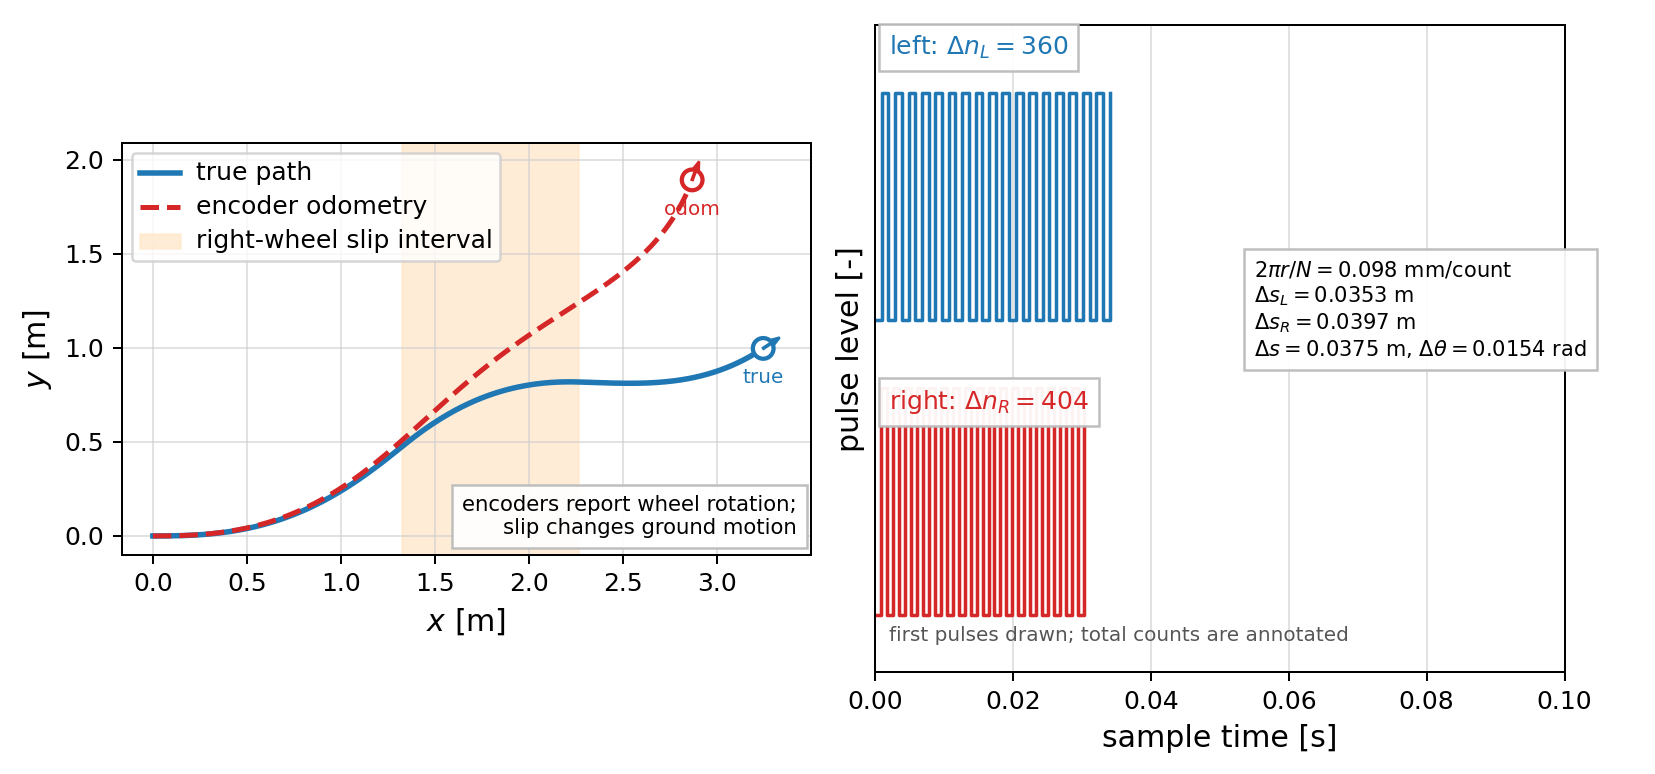
\includegraphics[width=0.95\linewidth,bb=0 0 1655 774]{figures/flow6_odometry_examples.png}
  \caption{差動駆動ロボットの真の軌跡とエンコーダオドメトリのずれ、および 1 サンプル内の左右エンコーダパルスの例。右車輪が床に対して滑ると、エンコーダは車輪の回転を数え続けるため、オドメトリは実際の床上移動より大きい右車輪距離を積分する。}
  \label{fig:flow-six-odometry-examples}
\end{figure}

図\ref{fig:flow-six-odometry-examples}の左図では、青線が床上の真の軌跡、赤破線がエンコーダから計算したオドメトリである。右車輪が滑った区間では、車輪は回っているのに床を押して進む距離が小さくなる。エンコーダはこの差を直接検出できないので、オドメトリは「車輪が地面を滑らず転がった」という仮定のもとで姿勢を更新し続ける。図が示しているのは、ミリメートル程度の車輪距離誤差でも、時間積分によってセンチメートルからデシメートル級の位置ずれに成長するという事実である。一方で、この図だけから滑りの物理原因や真の軌跡を実機上で知ることはできない。ここではシミュレーションなので青線を真値として描けるが、実機では別の測定を入れなければ、どちらの軌跡が床上の実際の動きに近いかをエンコーダだけで判定できない。

車輪半径を $r$ [m]、エンコーダの 1 回転あたりのパルス数を $N$ [count/rev] とする。サンプル時刻 $k$ から $k+1$ の間に左車輪で $\Delta n_L$ [count]、右車輪で $\Delta n_R$ [count] が数えられたとき、滑りがなく、半径の校正値も正しいという仮定のもとで、左右車輪の移動距離は
\begin{align}
  \Delta s_L&=\frac{2\pi r}{N}\Delta n_L,\\
  \Delta s_R&=\frac{2\pi r}{N}\Delta n_R
  \label{eq:wheel-pulse-distance}
\end{align}
である。係数 $2\pi r/N$ の単位は
\begin{equation}
  \frac{\mathrm{m/rev}}{\mathrm{count/rev}}
  =\mathrm{m/count}
\end{equation}
であり、パルス数を距離へ変換する換算係数になっている。たとえば $r=0.032\,\mathrm{m}$、$N=2048\,\mathrm{count/rev}$ なら
\begin{equation}
  \frac{2\pi r}{N}
  =
  \frac{2\pi\cdot0.032}{2048}
  =9.82\times10^{-5}\,\mathrm{m/count}
  =0.0982\,\mathrm{mm/count}
\end{equation}
である。

\begin{table}[tb]
  \centering
  \caption{1 サンプル $\Delta t=0.10\,\mathrm{s}$ におけるパルス数から姿勢増分までの計算例。}
  \label{tab:flow-six-encoder-step}
  \begin{tabular}{lll}
    \hline
    量 & 計算 & 値 \\
    \hline
    左車輪パルス & $\Delta n_L$ & $360\,\mathrm{count}$ \\
    右車輪パルス & $\Delta n_R$ & $404\,\mathrm{count}$ \\
    左車輪距離 & $9.82\times10^{-5}\cdot360$ & $0.0353\,\mathrm{m}$ \\
    右車輪距離 & $9.82\times10^{-5}\cdot404$ & $0.0397\,\mathrm{m}$ \\
    並進増分 & $(\Delta s_R+\Delta s_L)/2$ & $0.0375\,\mathrm{m}$ \\
    角度増分 & $(\Delta s_R-\Delta s_L)/b,\ b=0.280\,\mathrm{m}$ & $0.0154\,\mathrm{rad}$ \\
    \hline
  \end{tabular}
\end{table}

この表は、パルス数が多い右車輪のほうが長く進んだと推定され、その差が機体の向きの変化になることを数値で示している。サンプル幅で割れば車体速度と角速度も得られる。車輪間距離を $b$ [m] とし、車体中心を左右車輪の中点に置くと、サンプル内の平均速度は
\begin{align}
  v_k&=\frac{1}{2\Delta t}(\Delta s_R+\Delta s_L),\\
  \omega_k&=\frac{1}{b\Delta t}(\Delta s_R-\Delta s_L)
  \label{eq:diff-drive-kinematics}
\end{align}
である。表\ref{tab:flow-six-encoder-step}の値では
\begin{align}
  v_k&=\frac{0.0397+0.0353}{2\cdot0.10}
       =0.375\,\mathrm{m/s},\\
  \omega_k&=\frac{0.0397-0.0353}{0.280\cdot0.10}
       =0.154\,\mathrm{rad/s}
\end{align}
となる。ここで $\omega_k$ の符号は、右車輪が左車輪より長く進むと左向きに旋回するという座標系の取り方に対応している。

姿勢を $p_k=(x_k,y_k,\theta_k)$ と書く。$\theta_k$ は世界座標の $x$ 軸から見た車体前方の角度である。サンプル内で速度が一定に近いとみなせるなら、並進増分
\begin{equation}
  \Delta s_k=\frac{\Delta s_R+\Delta s_L}{2},
  \qquad
  \Delta\theta_k=\frac{\Delta s_R-\Delta s_L}{b}
\end{equation}
を使って、中点角度で
\begin{align}
  x_{k+1}
  &=x_k+\Delta s_k\cos\left(\theta_k+\frac{\Delta\theta_k}{2}\right),\\
  y_{k+1}
  &=y_k+\Delta s_k\sin\left(\theta_k+\frac{\Delta\theta_k}{2}\right),\\
  \theta_{k+1}
  &=\theta_k+\Delta\theta_k
  \label{eq:odometry-midpoint-step}
\end{align}
と積分する。この式は、車体がサンプル中に少し向きを変えることを、始点角度ではなく中点角度で代表させる近似である。たとえば $\theta_k=0.30\,\mathrm{rad}$ で表\ref{tab:flow-six-encoder-step}の増分を使うと、
\begin{align}
  x_{k+1}-x_k
  &=0.0375\cos(0.30+0.0154/2)
    =0.0357\,\mathrm{m},\\
  y_{k+1}-y_k
  &=0.0375\sin(0.30+0.0154/2)
    =0.0114\,\mathrm{m},\\
  \theta_{k+1}-\theta_k
  &=0.0154\,\mathrm{rad}
\end{align}
である。パルス数、車輪半径、車輪間距離、姿勢角がすべて具体的な単位を持つので、オドメトリは単なる幾何の公式ではなく、測定単位を姿勢単位へ変換する計算であることが明確になる。

この導出の重要な仮定は二つある。第一に、左右車輪が床に対して滑らず純転がりしていることである。第二に、半径 $r$、車輪間距離 $b$、パルス数 $N$、左右の取り付けが正しく校正されていることである。実際には、床材、加減速、旋回、荷重移動、タイヤ摩耗、左右半径差、バックラッシュ、量子化によって、$\Delta s_L,\Delta s_R$ は床上の移動距離からずれる。右車輪が $5\,\%$ だけ滑っているのにエンコーダ上は $0.040\,\mathrm{m}$ 進んだように記録されるなら、床上の右車輪距離は $0.038\,\mathrm{m}$ にしかならない。差は $0.002\,\mathrm{m}$ と小さいが、角度増分には
\begin{equation}
  \frac{0.002}{0.280}
  =0.0071\,\mathrm{rad}
  \simeq0.41^\circ
\end{equation}
として入る。これが何百サンプルも足し合わされると、位置のずれは無視できない大きさになる。

したがって、オドメトリは「短時間では強い、長時間では疑うべき」推定である。短いサンプルでは、パルス数から速度と角速度を高い時間分解能で得られる。ところが絶対位置を外部から測定していないため、滑りや校正誤差は積分で蓄積する。図\ref{fig:flow-six-odometry-examples}は、エンコーダ積分が有用であることと、エンコーダだけでは床上の真の姿勢を保証できないことを同時に示している。次に必要になるのは、車輪の回転とは別の物理量、たとえば角速度や重力方向を測るセンサであり、そこから IMU を用いた姿勢変化の推定へ進む。

\subsection{エンコーダ誤差とスリップによるセンサ追加の必要性}

直前までのオドメトリでは、左右の車輪エンコーダから得た回転量を地面上の移動量へ変換し、差動二輪ロボットの位置と方位角を逐次積分した。左右車輪の半径を $r_L,r_R$ [m]、車輪間距離を $b$ [m]、時刻 $k$ の短い区間における車輪角の増分を $\Delta\phi_{L,k},\Delta\phi_{R,k}$ [rad] とすると、すべりがなく、半径が正しく、パルス数が十分細かいという条件では
\begin{align}
  \Delta s_{L,k}&=r_L\Delta\phi_{L,k},&
  \Delta s_{R,k}&=r_R\Delta\phi_{R,k},\\
  \Delta s_k&=\frac{\Delta s_{R,k}+\Delta s_{L,k}}{2},&
  \Delta\theta_k&=\frac{\Delta s_{R,k}-\Delta s_{L,k}}{b}
\end{align}
で進む。ここで $\Delta s_{L,k},\Delta s_{R,k},\Delta s_k$ は [m]、$\Delta\theta_k$ は [rad] である。この式は、車輪の回転量と地面上の移動量が一対一に対応するという機械的な仮定を含んでいる。次に必要になるのは、この仮定がどの程度の速さで破れるかを数値で見ることである。

まず車輪半径の設定誤差を考える。オドメトリが使う半径を
\begin{equation}
  \hat{r}_i=(1+\epsilon_i)r_i,\qquad i\in\{L,R\}
\end{equation}
と書くと、推定された車輪移動量は
\begin{equation}
  \hat{\Delta s}_{i,k}
  =
  \hat{r}_i\Delta\phi_{i,k}
  =
  (1+\epsilon_i)\Delta s_{i,k}
\end{equation}
である。したがって、半径誤差だけによる方位角増分のずれは
\begin{equation}
  \hat{\Delta\theta}_k-\Delta\theta_k
  =
  \frac{\epsilon_R\Delta s_{R,k}-\epsilon_L\Delta s_{L,k}}{b}
\end{equation}
となる。左右が同じ割合でずれると主に距離の尺度が変わり、左右差をもつと方位角が少しずつ曲がる。たとえば $b=0.32\,\mathrm{m}$ のロボットで、右車輪だけが $1.0\,\%$ 大きく見積もられ、左右とも地面上で $2.00\,\mathrm{m}$ 進んだ場合、右車輪距離の過大評価は $0.020\,\mathrm{m}$ であり、方位角のずれは
\begin{equation}
  \frac{0.020}{0.32}=0.0625\,\mathrm{rad}
  \simeq 3.58^\circ
\end{equation}
になる。半径誤差は小さく見えても、走行距離に比例して蓄積する。

次に、パルス量子化を入れる。1 回転あたりのエンコーダ分解能を $N$ [count/rev] とすると、1 count が表す車輪外周上の距離は
\begin{equation}
  q=\frac{2\pi r}{N}\quad[\mathrm{m/count}]
\end{equation}
である。$r=0.050\,\mathrm{m}$、$N=360\,\mathrm{count/rev}$ なら
\begin{equation}
  q
  =
  \frac{2\pi\cdot0.050}{360}
  =
  8.73\times10^{-4}\,\mathrm{m/count}
  =
  0.873\,\mathrm{mm/count}
\end{equation}
である。累積 count を整数に丸めて読むと、各車輪の距離換算残差は高々約 $q/2=0.436\,\mathrm{mm}$ である。左右の丸め残差が反対符号になった瞬間の方位角残差は、おおまかに
\begin{equation}
  \abs{\delta\theta_q}
  \le
  \frac{q}{b}
  =
  \frac{0.873\times10^{-3}}{0.32}
  =
  2.73\times10^{-3}\,\mathrm{rad}
  \simeq0.156^\circ
\end{equation}
である。量子化は 1 回の読み取りでは小さいが、低速時には速度推定を階段状にし、微小な旋回や停止直前の判定を粗くする。

最後に、短いスリップ区間を入れる。左車輪が回転した外周距離を $r_L\Delta\phi_{L,k}$ とし、地面に実際に伝わった割合を $\lambda_{L,k}\in[0,1]$ と書くと、
\begin{equation}
  \Delta s^{\mathrm{ground}}_{L,k}
  =
  \lambda_{L,k}r_L\Delta\phi_{L,k}
\end{equation}
である。エンコーダは車輪軸の回転を測るので、$\lambda_{L,k}$ を直接測っていない。左車輪だけがすべった区間では、エンコーダが使う距離と地面上の距離の差
\begin{equation}
  \Delta s_{\mathrm{loss},k}
  =
  (1-\lambda_{L,k})r_L\Delta\phi_{L,k}
\end{equation}
が残り、真の旋回増分とエンコーダ由来の旋回増分の差は近似的に
\begin{equation}
  \Delta\theta_{\mathrm{true},k}
  -
  \Delta\theta_{\mathrm{enc},k}
  \simeq
  \frac{\Delta s_{\mathrm{loss},k}}{b}
\end{equation}
となる。半径誤差や量子化はエンコーダ値の換算に現れるが、スリップは「車輪は回ったが、機体は同じだけ進まなかった」という地面との相互作用に現れる。

図\ref{fig:flow6-encoder-slip-examples}は、$b=0.32\,\mathrm{m}$、$r=0.050\,\mathrm{m}$、$N=360\,\mathrm{count/rev}$ の差動二輪ロボットを 8 s 走らせた計算例である。$3.20$ s から $3.80$ s まで左車輪だけがすべり、車輪が回した距離の $60\,\%$ だけが地面へ伝わるとした。通常のエンコーダオドメトリは count から進んだつもりの経路を積分するため、すべり区間のあとも真の経路から離れたままになる。さらに、左半径を $+1.5\,\%$、右半径を $-1.0\,\%$ だけ誤って換算すると、方位角のずれが同じ方向に重なり、8 s 後の位置誤差は $0.390\,\mathrm{m}$ から $0.676\,\mathrm{m}$ へ増える。方位角誤差も $-14.53^\circ$ から $-26.96^\circ$ へ広がる。

\begin{figure}[tb]
\centering
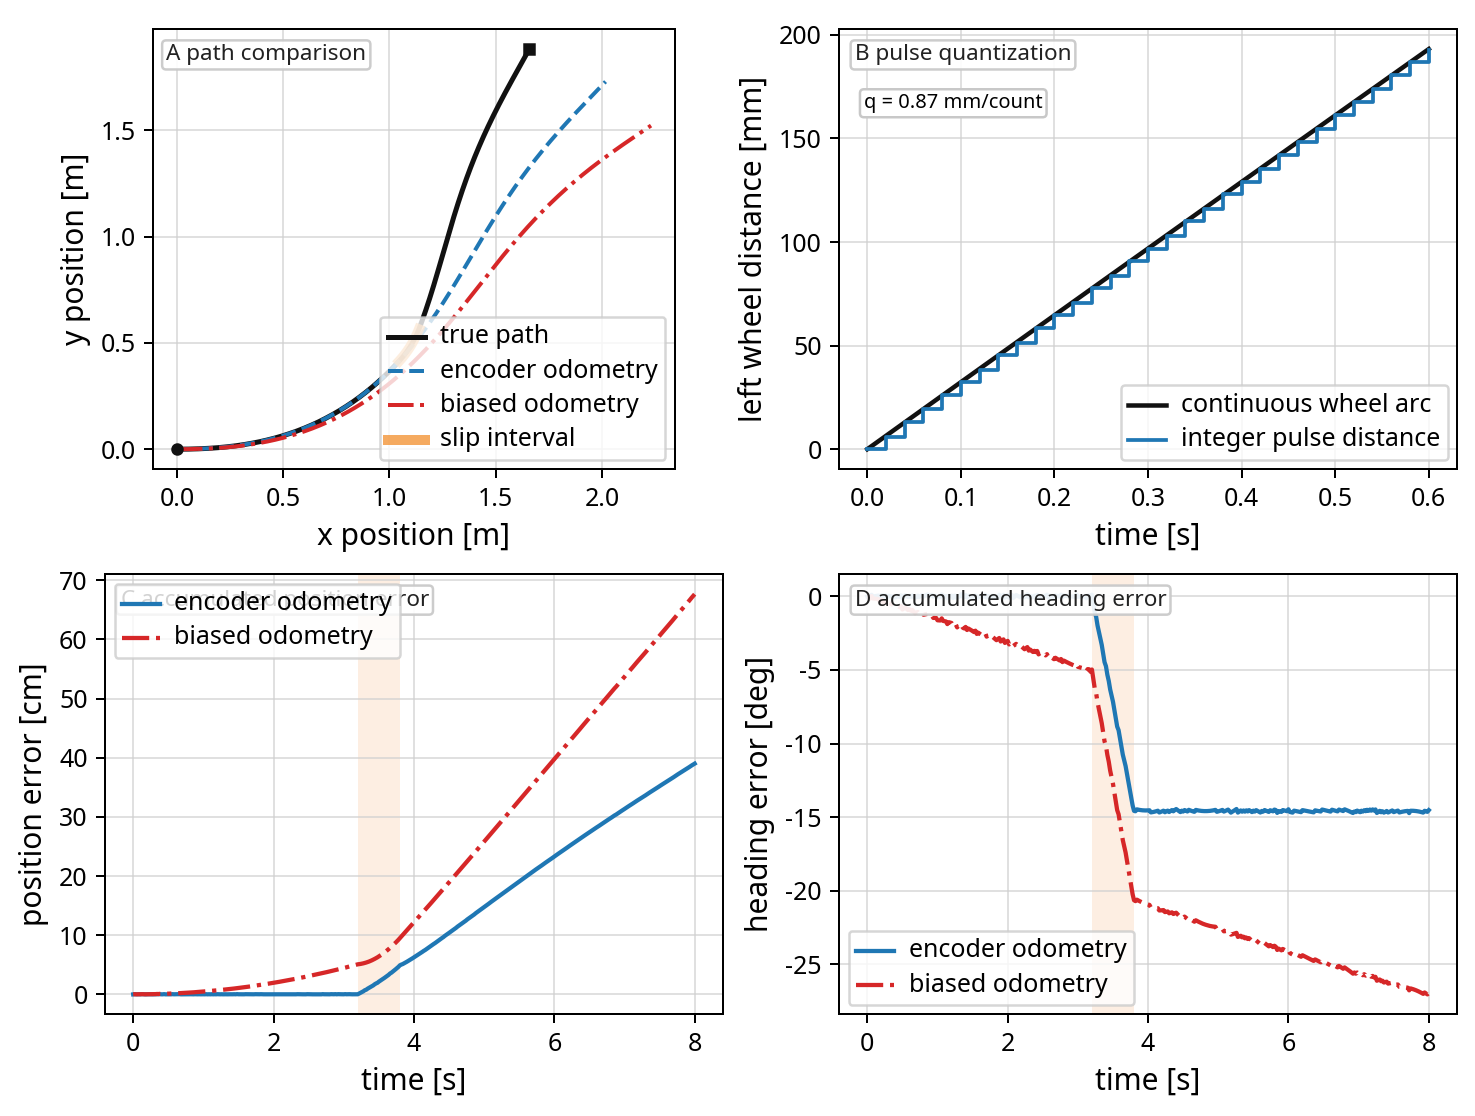
\includegraphics[width=0.95\linewidth,bb=0 0 1476 1116]{figures/flow6_encoder_slip_examples.png}
\caption{差動二輪ロボットにおける真の経路、通常のエンコーダオドメトリ、半径誤差を重ねたオドメトリの比較。左車輪は $3.20$--$3.80\,\mathrm{s}$ だけすべり、車輪外周の移動量 $0.204\,\mathrm{m}$ のうち $0.081\,\mathrm{m}$ が地面上の移動に変換されない。量子化の 1 count は $0.873\,\mathrm{mm}$ であり、短時間の距離推定を階段状にする。}
\label{fig:flow6-encoder-slip-examples}
\end{figure}

\begin{table}[tb]
\centering
\footnotesize
\setlength{\tabcolsep}{3pt}
\begin{tabular}{>{\raggedright\arraybackslash}p{0.20\linewidth}>{\raggedright\arraybackslash}p{0.25\linewidth}>{\raggedright\arraybackslash}p{0.23\linewidth}>{\raggedright\arraybackslash}p{0.22\linewidth}}
\hline
要因 & 代表値 & 距離への影響 & 方位角への影響\\
\hline
半径設定ずれ & 右だけ $+1.0\,\%$, $s=2.00\,\mathrm{m}$ & $+20\,\mathrm{mm}$ & $0.020/0.32=3.58^\circ$\\
パルス量子化 & $q=0.873\,\mathrm{mm/count}$ & $\le0.436\,\mathrm{mm}$ & $\le0.156^\circ$\\
左車輪スリップ & $\lambda=0.60$, 回転距離 $0.204\,\mathrm{m}$ & 損失 $0.081\,\mathrm{m}$ & $0.081/0.32=14.6^\circ$\\
\hline
\end{tabular}
\caption{半径誤差、パルス量子化、短時間スリップが距離と方位角へ与える代表的な大きさ。スリップは短時間でも方位角に大きく効き、しかもエンコーダ count だけでは検出できない。}
\label{tab:flow6-encoder-error-contributions}
\end{table}

表\ref{tab:flow6-encoder-error-contributions}の値は、エンコーダだけで自己位置を閉じると何が失われるかを分けている。半径誤差は、同じ count を何 m と読むかの尺度誤差である。量子化は、連続的な車輪角を整数 count に丸めることによる読み取り誤差である。スリップはこれらと性質が異なり、count 列そのものは正常に見えているのに、地面上の移動量が同じでなくなる。エンコーダ値だけを入力にして
\begin{equation}
  (x_k,y_k,\theta_k)
  =
  F\left((x_{k-1},y_{k-1},\theta_{k-1}),\Delta n_{L,k},\Delta n_{R,k}\right)
\end{equation}
と積分している限り、同じ $\Delta n_{L,k},\Delta n_{R,k}$ から「車輪が地面を押して進んだ場合」と「車輪が空転気味に回った場合」を区別できない。方位角についても同じで、左右 count の差から積分した $\theta$ がゆっくりずれても、エンコーダだけでは外部基準に対する方位角の残差を作れない。

この不可観測なずれが、次に慣性センサを加える理由である。IMU は車輪の回転ではなく、機体に取り付けたセンサとして角速度や加速度に対応する信号を出す。もちろん IMU にもバイアス、ノイズ、重力方向との混同があるため、単体で完全な位置を与えるわけではない。それでも、車輪 count と独立した方位角変化の手掛かりを持つため、スリップや方位角ドリフトを検出・補正するための別の観測経路になる。次の段階では、IMU の式を急いで導入する前に、ジャイロ積分、加速度計が見る重力、バイアスとノイズの蓄積を順に調べ、エンコーダだけでは閉じなかった残差をどの信号で見るのかを明確にする。

\subsection{IMU 軸とジャイロ積分}

車輪エンコーダだけで差動二輪ロボットの姿勢を積分すると、左右輪の移動量差からヨー角を計算できる。しかし、片輪が短い時間だけ空転したり、床面で横滑りしたりすると、エンコーダは「車輪が進んだ量」を正しく数えても、「機体が床に対して向きを変えた量」を正しく表さない。オドメトリの式そのものは滑らかな軌跡を出すため、推定された向きのずれはすぐには見えにくい。数 m 走った後に、地図上の経路だけが少しずつ回転しているように見えることがある。この制限を補うため、車輪ではなく機体に固定された座標軸で角速度を測る IMU を導入する。

ここで必要なのは IMU の分類表ではなく、機体に貼り付いた測定軸である。床に固定された慣性系を $\{I\}$ とし、ロボットの中心に固定された機体系を $\{B\}$ とする。平面走行では、$\{B\}$ の $x_B$ 軸を前方、$y_B$ 軸を左方向、$z_B$ 軸を上向きに取る。慣性系の $x_I$ 軸から機体系の $x_B$ 軸まで反時計回りに測った角をヨー角 $\psi$ [rad] とする。ロボットが床から浮かず、ロールとピッチが小さい範囲では、$z_B$ 軸まわりの角速度 $\omega_z^B$ [rad/s] はヨー角の時間微分
\begin{equation}
  \dot{\psi}(t)=\omega_z^B(t)
\end{equation}
として扱える。この近似は、二輪ロボットの進行方向と横方向を機体に結び付け、地図上の向きだけを一つの角度で追うための平面モデルである。

ジャイロは角速度そのものを返すのではなく、バイアスとノイズを含む測定値を返す。時刻 $t_k=kT_s$、サンプリング周期 $T_s$ [s] の離散測定を
\begin{equation}
  \omega_{z,m,k}^B
  =
  \omega_z^B(t_k)+b_g+n_{g,k}
\end{equation}
と書く。$\omega_{z,m,k}^B$ は測定された $z_B$ 軸まわり角速度 [rad/s]、$b_g$ は一定とみなしたジャイロバイアス [rad/s]、$n_{g,k}$ は平均 0 の測定ノイズ [rad/s] である。角速度を時間で積分すると角度になるので、単位は
\begin{equation}
  [\mathrm{rad/s}]\,[\mathrm{s}]=[\mathrm{rad}]
\end{equation}
とそろう。

連続時間では、初期時刻 $t_0$ から時刻 $t$ までのヨー角は
\begin{equation}
  \psi(t)
  =
  \psi(t_0)+\int_{t_0}^{t}\omega_z^B(\tau)\,\dd\tau
\end{equation}
である。サンプリングされた測定値を 1 サンプルの間だけ一定とみなすと、ジャイロ積分は
\begin{equation}
  \hat{\psi}_k
  =
  \hat{\psi}_{k-1}
  +
  \left(\omega_{z,m,k}^B-\hat{b}_g\right)T_s
\end{equation}
となる。$\hat{b}_g$ はバイアスの補正値である。右辺の括弧の中は [rad/s]、$T_s$ は [s] なので、1 ステップで加える量は [rad] である。エンコーダのスリップで壊れた「車輪から見た向き」ではなく、機体に固定されたジャイロの角速度を積分して向きを進める点が、IMU を入れる最初の利点である。

ただし、ジャイロ積分は絶対的な方位を直接測っているわけではない。真の角度を同じサンプリングで
\begin{equation}
  \psi_k
  \simeq
  \psi_{k-1}+\omega_z^B(t_k)T_s
\end{equation}
と近似し、誤差を $e_{\psi,k}=\hat{\psi}_k-\psi_k$ と置く。測定式と積分式を代入して差を取ると
\begin{align}
  e_{\psi,k}
  &=
  e_{\psi,k-1}
  +
  \left(b_g-\hat{b}_g+n_{g,k}\right)T_s
\end{align}
である。バイアスを補正しない場合は $\hat{b}_g=0$ であり、$E[n_{g,k}]=0$、$e_{\psi,0}=0$ とすれば
\begin{align}
  E[e_{\psi,k}]
  &=
  E[e_{\psi,k-1}]+b_gT_s\\
  &=
  kb_gT_s\\
  &=
  b_g t_k
\end{align}
となる。一定のバイアスは 1 サンプルごとには小さくても、時間に比例する角度誤差として蓄積する。

図\ref{fig:flow-six-imu-gyro-examples}は、機体系に固定された IMU の軸と、一定バイアスを補正しないときのヨー角誤差を並べたものである。右図では $T_s=0.01\,\mathrm{s}$ とし、$b_g=0.1^\circ/\mathrm{s}$、$0.5^\circ/\mathrm{s}$、$1.5^\circ/\mathrm{s}$ の三つを比較している。$0.5^\circ/\mathrm{s}$ は 100 Hz の 1 サンプルでは $0.005^\circ$ しか増えないが、60 s 後には
\begin{equation}
  0.5^\circ/\mathrm{s}\times 60\,\mathrm{s}=30^\circ
\end{equation}
の向き誤差になる。$1.5^\circ/\mathrm{s}$ なら同じ 60 s で $90^\circ$ まで増える。小さな直流成分が積分で大きな低周波誤差になるため、ジャイロはスリップに強い一方で、バイアスを無視したまま長時間の方位基準として使うことはできない。

\begin{figure}[tb]
\centering
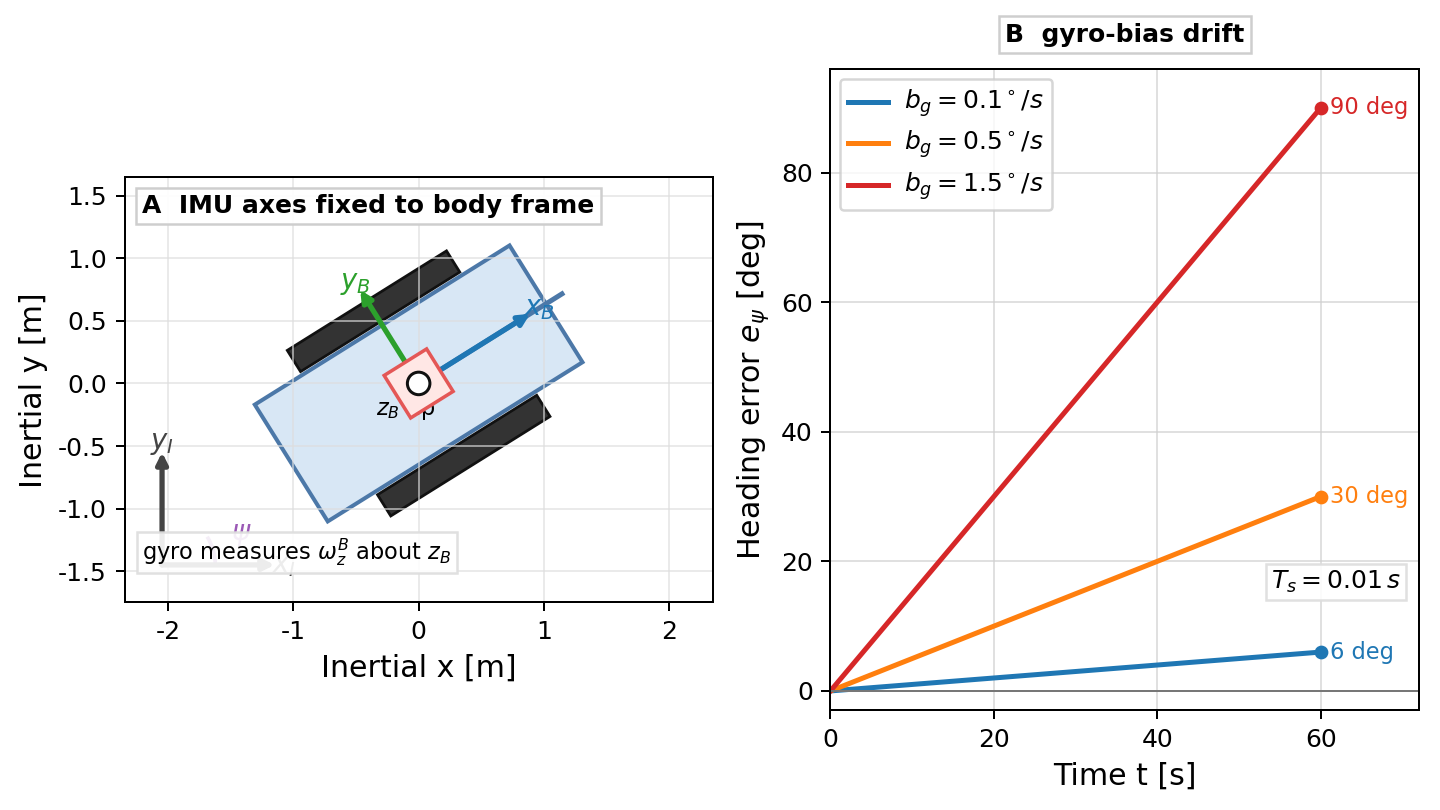
\includegraphics[width=0.95\linewidth,bb=0 0 1440 810]{figures/flow6_imu_gyro_examples.png}
\caption{差動二輪ロボットに固定した IMU の機体軸と、一定ジャイロバイアスによるヨー角誤差の蓄積。左図では IMU が機体系 $\{B\}$ に固定され、$z_B$ 軸まわりの角速度を測る。右図では $T_s=0.01\,\mathrm{s}$ でジャイロを積分し、バイアスが $0.1^\circ/\mathrm{s}$、$0.5^\circ/\mathrm{s}$、$1.5^\circ/\mathrm{s}$ のとき、誤差がそれぞれ 60 s 後に $6^\circ$、$30^\circ$、$90^\circ$ へ達することを示している。}
\label{fig:flow-six-imu-gyro-examples}
\end{figure}

この比較から、IMU を入れる意味は二つに分かれる。第一に、車輪が滑った瞬間でも、機体が実際に回った角速度を直接測れるので、エンコーダだけの向き推定よりスリップに引きずられにくい。第二に、ジャイロだけではバイアスが積分されるため、長時間の向きには別の情報が必要になる。加速度計が測る比力と重力方向からロール・ピッチを扱う話はこの後の段階で扱うが、ここではまだその導出には進まない。まず押さえるべき事実は、IMU の軸は機体に固定されており、ジャイロ測定は角速度として有用だが、積分するとバイアスが角度誤差へ変わるという点である。

\subsection{加速度計による重力投影と傾斜推定}

車輪オドメトリは車輪が地面を正しく転がることに依存し、ジャイロ積分は角速度バイアスを時間とともに角度誤差へ変える。IMU の中で、ジャイロとは別の情報を与えるのが加速度計である。ただし、加速度計の出力は「物体の並進加速度そのもの」ではない。加速度計が直接測る量は、センサ内部の質量に働く支持力を質量で割った量、すなわち比力（specific force）であり、単位は加速度と同じ $[\mathrm{m/s^2}]$ である。センサが机の上で静止しているとき、慣性座標系での並進加速度は 0 であるにもかかわらず、鉛直上向きにほぼ $9.81\,\mathrm{m/s^2}$ の大きさが出る。この値は、重力によって自由落下しないように机がセンサを支えていることを表す。

慣性座標系を $\{I\}$、IMU に固定した機体系を $\{B\}$ とし、機体系から慣性系への姿勢を $R^I_B$ と書く。慣性系で表した重力加速度を
\begin{equation}
  g^I=\begin{bmatrix}0\\0\\-g\end{bmatrix},
  \qquad
  g=9.80665\,\mathrm{m/s^2}
\end{equation}
とする。IMU 原点の並進加速度を $a^I$ $[\mathrm{m/s^2}]$、加速度計バイアスを $b_a^B$、ノイズを $n_a^B$ とすれば、加速度計の測定値は
\begin{equation}
  a_m^B
  =
  (R^I_B)^\T\left(a^I-g^I\right)+b_a^B+n_a^B
  \label{eq:accelerometer-specific-force}
\end{equation}
で表せる。式\eqref{eq:accelerometer-specific-force}の $a^I-g^I$ が比力である。重力を含む「見かけの加速度」ではなく、重力を差し引いた運動加速度を作るために必要な支持力を、機体系成分で表している。

低速で静止に近い時間帯では、$a^I\simeq0$ とみなせる。このとき
\begin{equation}
  a_m^B\simeq -(R^I_B)^\T g^I
\end{equation}
となり、加速度計は重力ベクトルの向きそのものではなく、重力を打ち消す比力の機体系への投影を返す。したがって、重力の大きさが既知で、並進加速度が小さいという条件が成り立つ間は、加速度計からロール角とピッチ角を幾何的に取り出せる。

ZYX オイラー角で
\begin{equation}
  R^I_B=R_z(\psi)R_y(\theta)R_x(\phi)
\end{equation}
とし、静止に近く、バイアスとノイズをいったん無視する。重力は慣性系の $z$ 軸方向だけを向くので、ヨー角 $\psi$ は重力投影に現れない。計算すると
\begin{align}
  a_m^B
  &\simeq
  - (R^I_B)^\T g^I\\
  &=
  \begin{bmatrix}
    -g\sin\theta\\
    g\sin\phi\cos\theta\\
    g\cos\phi\cos\theta
  \end{bmatrix}.
  \label{eq:accelerometer-gravity-projection}
\end{align}
この式から、ZYX のロール・ピッチ表示で分母 $\sqrt{(a_{m,y}^B)^2+(a_{m,z}^B)^2}$ が 0 に近くない枝では
\begin{align}
  \hat{\phi}_a
  &=
  \operatorname{atan2}\left(a_{m,y}^B,a_{m,z}^B\right),\\
  \hat{\theta}_a
  &=
  \operatorname{atan2}\left(-a_{m,x}^B,
    \sqrt{(a_{m,y}^B)^2+(a_{m,z}^B)^2}\right)
  \label{eq:accelerometer-roll-pitch}
\end{align}
というロール・ピッチ推定値が得られる。式\eqref{eq:accelerometer-roll-pitch}は、重力方向に対して機体がどの向きに傾いているかを、三つの加速度計軸への投影比として定式化したものである。一方、重力ベクトルのまわりの回転であるヨー角は、重力投影だけでは変わらない。加速度計だけでロールとピッチに強い手がかりが得られても、方位までは拘束できない。

平面内のピッチだけに絞ると、導出はさらに見やすい。$\phi=0$、$\psi=0$ とすれば
\begin{equation}
  a_{m,x}^B=-g\sin\theta,\qquad
  a_{m,z}^B=g\cos\theta
\end{equation}
である。したがって
\begin{equation}
  \hat{\theta}_a
  =
  \operatorname{atan2}\left(-a_{m,x}^B,a_{m,z}^B\right)
  =
  \operatorname{atan2}\left(g\sin\theta,g\cos\theta\right)
  =
  \theta
\end{equation}
となる。小角では $a_{m,x}^B\simeq -g\theta$ なので、$x$ 軸の比力を $g$ で割るだけでも傾斜角の一次近似が得られる。この簡潔さが、加速度計を傾斜センサとして使える理由である。

しかし、同じ式は限界も示す。機体が前方へ加速しており、その機体系 $x$ 軸成分を $a_\parallel$ $[\mathrm{m/s^2}]$ とする。重力投影にこの並進成分が加わるので
\begin{equation}
  a_{m,x}^B=a_\parallel-g\sin\theta,\qquad
  a_{m,z}^B=g\cos\theta
\end{equation}
となる。この測定値を静止時の式へそのまま代入すると
\begin{equation}
  \hat{\theta}_a
  =
  \operatorname{atan2}\left(g\sin\theta-a_\parallel,g\cos\theta\right)
  \label{eq:accelerometer-contaminated-tilt}
\end{equation}
である。小角かつ $\abs{a_\parallel}\ll g$ なら
\begin{equation}
  \hat{\theta}_a-\theta
  \simeq
  -\frac{a_\parallel}{g}
\end{equation}
となる。たとえば $a_\parallel=1.6\,\mathrm{m/s^2}$ の加速は、約 $-0.163\,\mathrm{rad}$、すなわち約 $-9.3^\circ$ の偽の傾斜として現れる。ロボットが発進・停止・旋回でこの程度の加速度を受けるなら、加速度計の傾斜値をそのまま姿勢として使うと、真の姿勢変化より大きな誤差を一時的に作る。

\begin{figure}[tb]
\centering
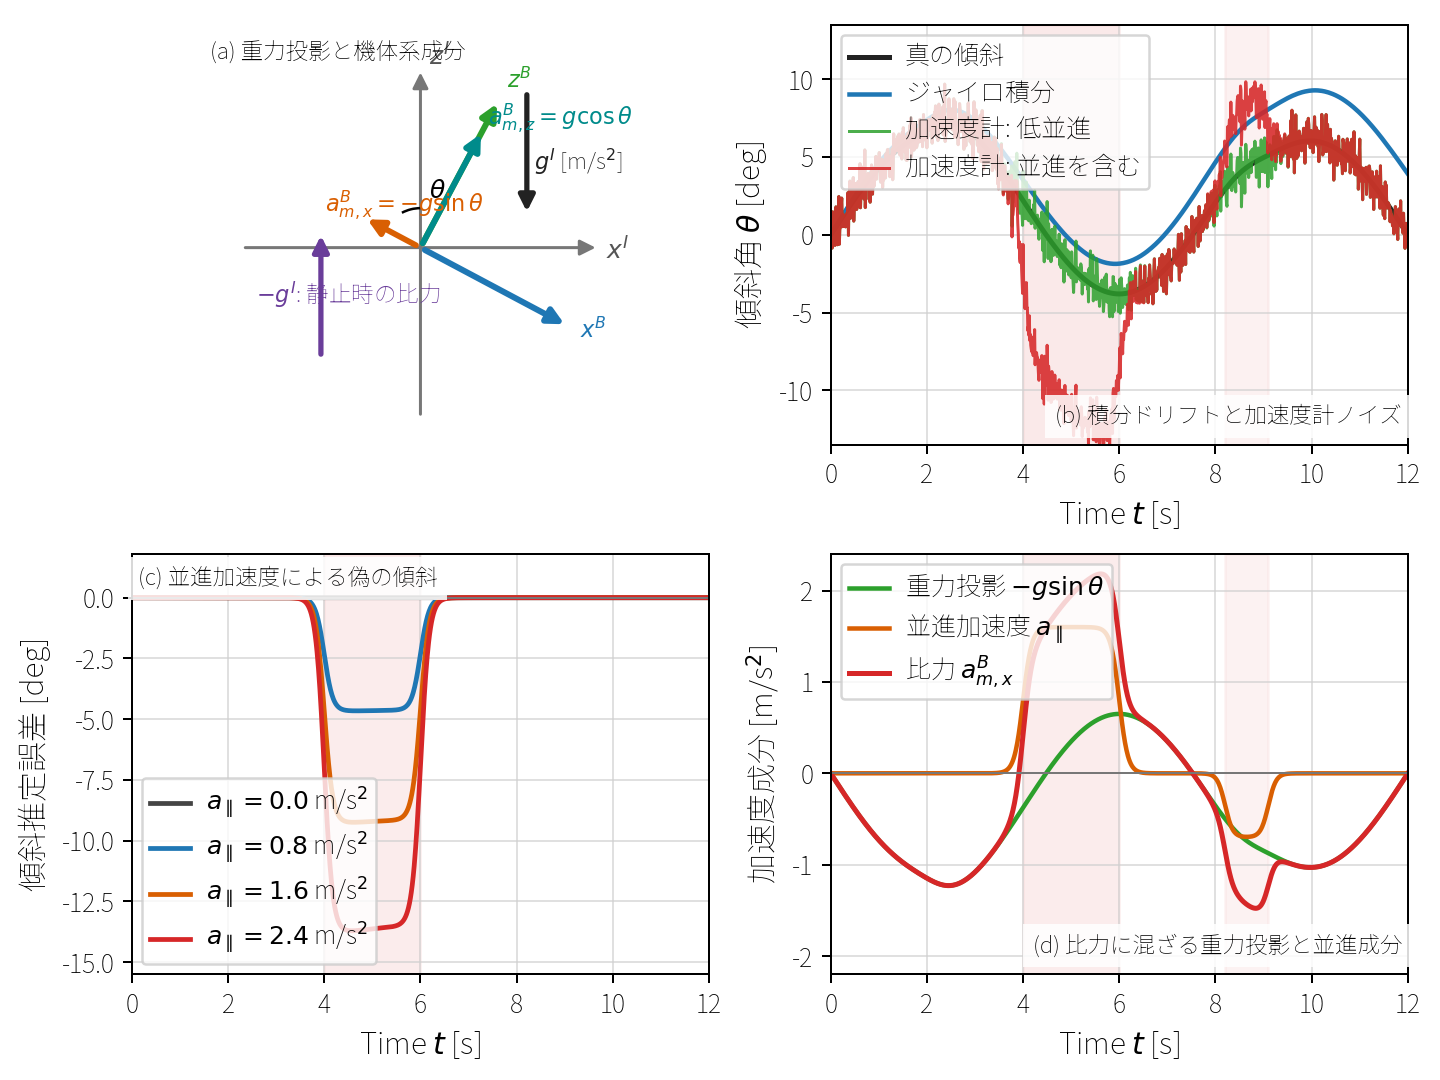
\includegraphics[width=0.95\linewidth,bb=0 0 1440 1080]{figures/flow6_accelerometer_tilt_examples.png}
\caption{加速度計による重力投影と傾斜推定の限界。左上は、静止時の比力が機体系の $x^B,z^B$ 軸へ投影され、$a_{m,x}^B=-g\sin\theta$、$a_{m,z}^B=g\cos\theta$ になる幾何である。右上は、真の傾斜、ジャイロ積分、低並進時の加速度計傾斜、並進加速度を含む加速度計傾斜を比較している。左下は $a_\parallel=0.0,0.8,1.6,2.4\,\mathrm{m/s^2}$ の変化による偽の傾斜誤差、右下は比力の $x$ 軸成分が重力投影と並進加速度の和として現れることを示す。}
\label{fig:flow6-accelerometer-tilt-examples}
\end{figure}

図\ref{fig:flow6-accelerometer-tilt-examples}の上段を比較すると、ジャイロ積分は短時間では滑らかに真の傾斜を追うが、一定の角速度バイアスによってゆっくりずれていく。加速度計から作った傾斜は積分を使わないのでバイアス性の角度ドリフトを持ちにくい一方、白色ノイズによって細かく揺れる。さらに、赤く示した並進加速度の時間帯では、式\eqref{eq:accelerometer-contaminated-tilt}の $a_\parallel/g$ に対応する誤差が乗り、実際には傾いていない向きの傾斜として推定される。下段のパラメータ変化では、$a_\parallel$ を大きくするほど偽の傾斜がほぼ比例して増え、$2.4\,\mathrm{m/s^2}$ では $14^\circ$ 程度のずれになる。

この結果から、ジャイロと加速度計は同じ角度を別々に測っているのではなく、互いに異なる弱点を持つ情報源であることが分かる。ジャイロ積分は高周波の姿勢変化を滑らかに保つが、低周波ではバイアスが角度ドリフトとして蓄積する。加速度計の重力投影は長時間の傾き基準を与えるが、ノイズと並進加速度に弱い。したがって次の段階では、低周波側では加速度計の重力基準を使い、高周波側ではジャイロ積分を使う相補フィルタを構成する。

\subsection{相補フィルタと共分散で表す残差不確かさ}

差動二輪ロボットや小型姿勢実験で IMU を使うと、最初に観測される限界は二つに分かれる。ジャイロの角速度は短い時間では滑らかで、ロボットが加速しても重力以外の力を直接は角度に混ぜない。しかし、角速度に小さなバイアスが含まれると、積分した角度はゆっくり片側へ流れていく。一方、加速度計から作る傾きは、静止に近いときには重力方向から絶対的な角度を与えるが、並進加速度や振動がある区間では、重力ではない加速度まで傾きとして解釈してしまう。したがって、ジャイロだけでは低周波のドリフトが残り、加速度計だけでは高周波のノイズと加速時の外乱が残る。

ここでは、一軸の小さな傾き $\theta$ を対象にする。サンプリング周期を $\Delta t$、ジャイロ測定を $\omega_{m,k}$、加速度計から作った傾き測定を $\theta_{\mathrm{acc},k}$ と置く。測定の典型的な近似は
\begin{align}
  \omega_{m,k}
  &=\dot{\theta}_k+b_k+n_{g,k},\\
  \theta_{\mathrm{acc},k}
  &=\theta_k+n_{a,k}+d_{a,k}
\end{align}
である。$b_k$ はゆっくり変化するジャイロバイアス、$n_{g,k}$ と $n_{a,k}$ は零平均の測定ノイズ、$d_{a,k}$ は並進加速度や振動によって加速度計の傾き換算へ混ざる成分である。ジャイロだけで
\begin{equation}
  \hat{\theta}^{g}_k
  =
  \hat{\theta}^{g}_{k-1}+\omega_{m,k}\Delta t
\end{equation}
と積分すると、$b_k$ の和が角度へ蓄積する。反対に $\theta_{\mathrm{acc},k}$ をそのまま使うと、$n_{a,k}$ と $d_{a,k}$ が直接角度推定へ入る。図\ref{fig:flow6-complementary-covariance-examples}は、この二つの失敗を同じ時系列に置き、固定相補フィルタがどこまで修正し、どの不確かさを残すかを示している。

\begin{figure}[tb]
  \centering
  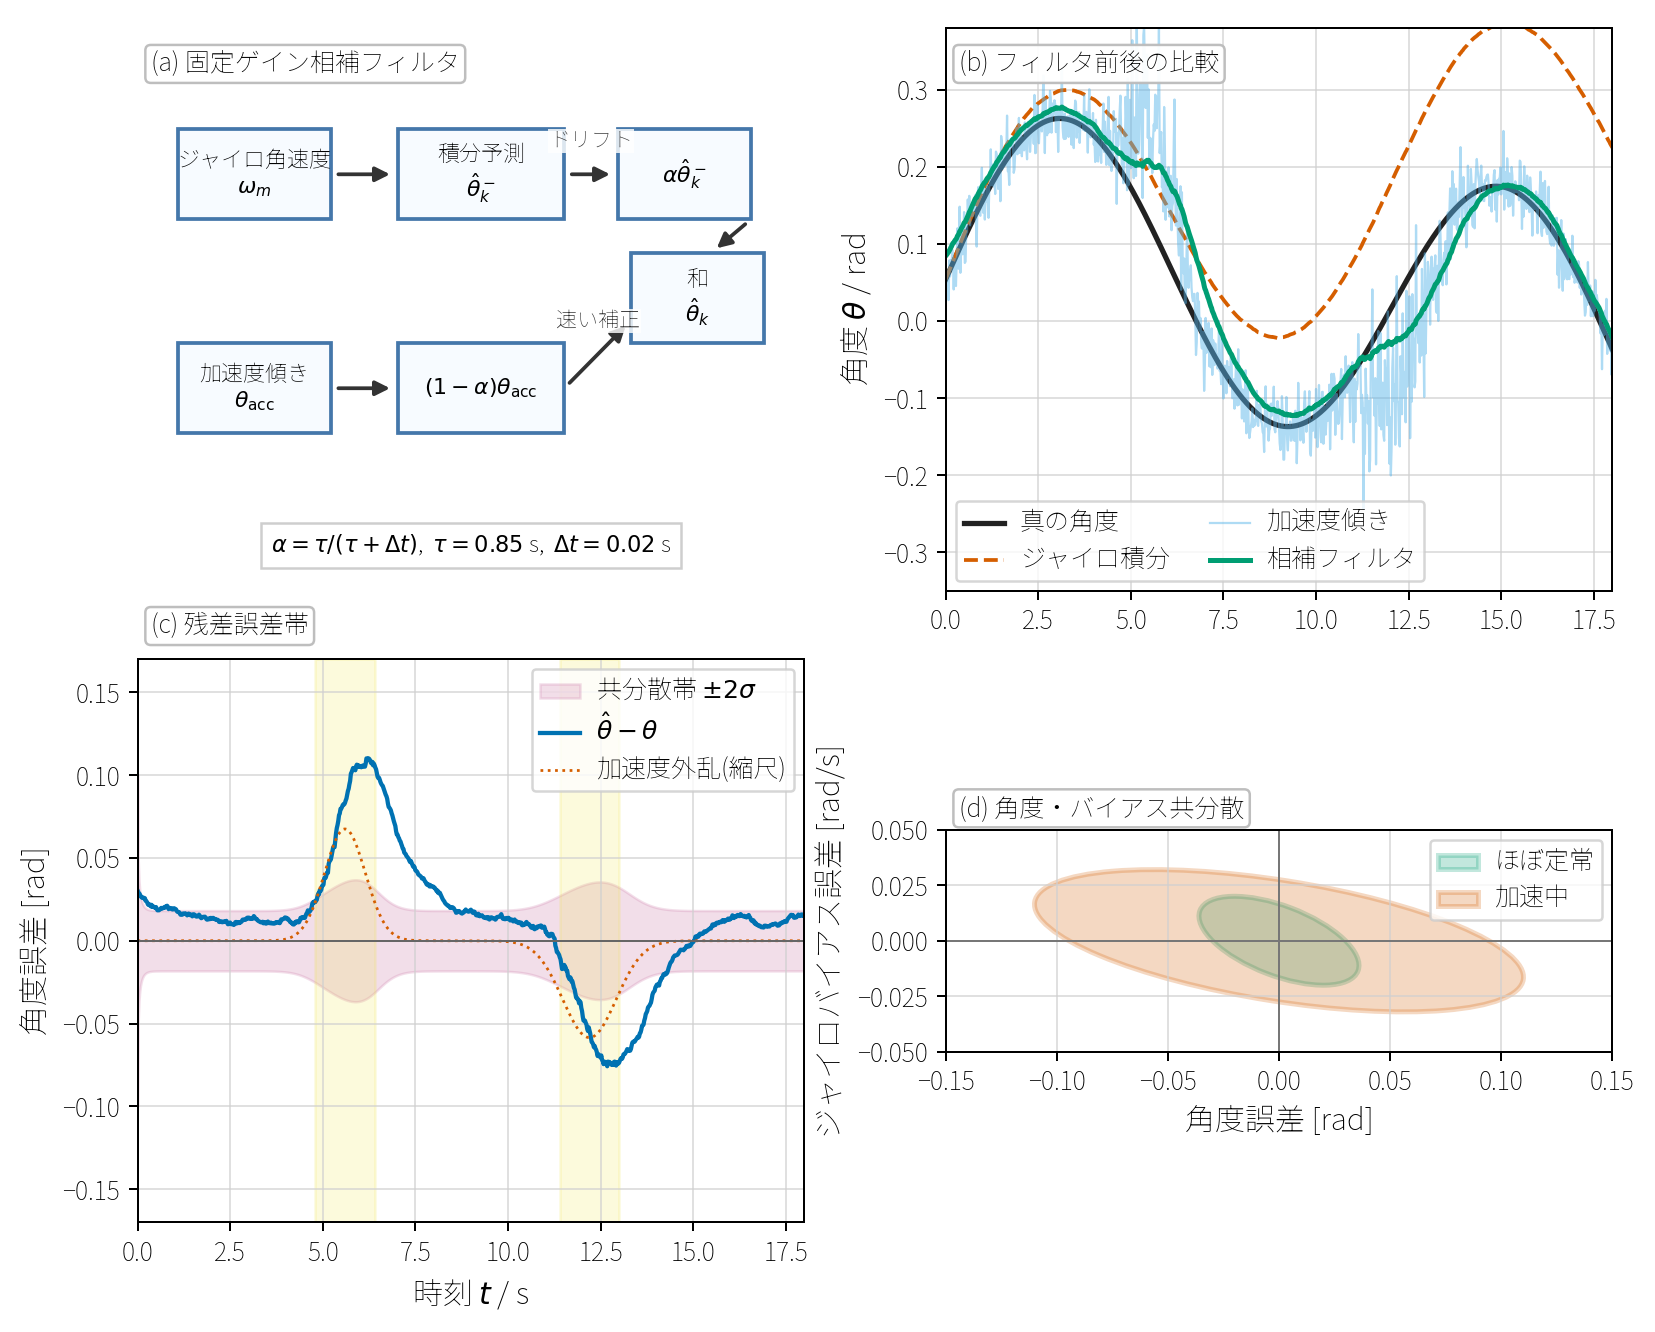
\includegraphics[width=0.98\linewidth]{figures/flow6_complementary_covariance_examples.png}
  \caption{ジャイロ積分、加速度計傾き、相補フィルタ、残差不確かさの関係。左上は固定係数の信号経路、右上はドリフトと加速度外乱を含む測定の前後比較、左下はフィルタ後の残差と共分散帯、右下は角度誤差とジャイロバイアス誤差の楕円表示である。加速区間では加速度計の見かけの傾きが悪化し、固定係数のままでは信頼度の変化を推定器の内部状態として保持できない。}
  \label{fig:flow6-complementary-covariance-examples}
\end{figure}

相補フィルタは、ジャイロ積分の低周波ドリフトと、加速度計傾きの高周波ノイズを互いに補わせる固定ゲインの推定器として書ける。連続時間で
\begin{equation}
  \dot{\hat{\theta}}
  =
  \omega_m+\frac{1}{\tau}
  \left(\theta_{\mathrm{acc}}-\hat{\theta}\right)
\end{equation}
と置くと、$\omega_m$ で角度を進めながら、時定数 $\tau$ で加速度計の傾きへ戻す一次遅れの補正になっている。この式を、補正項だけ後退 Euler で離散化すると
\begin{align}
  \hat{\theta}_k
  &=
  \hat{\theta}_{k-1}+\omega_{m,k}\Delta t
  +\frac{\Delta t}{\tau}
  \left(\theta_{\mathrm{acc},k}-\hat{\theta}_k\right),\\
  \left(1+\frac{\Delta t}{\tau}\right)\hat{\theta}_k
  &=
  \hat{\theta}_{k-1}+\omega_{m,k}\Delta t
  +\frac{\Delta t}{\tau}\theta_{\mathrm{acc},k},\\
  \hat{\theta}_k
  &=
  \alpha
  \left(\hat{\theta}_{k-1}+\omega_{m,k}\Delta t\right)
  +(1-\alpha)\theta_{\mathrm{acc},k}
\end{align}
を得る。ただし、この離散化では
\begin{equation}
  \alpha=\frac{\tau}{\tau+\Delta t},
  \qquad
  1-\alpha=\frac{\Delta t}{\tau+\Delta t}
\end{equation}
である。$\tau$ を大きくすると $\alpha$ は 1 に近づき、ジャイロ積分を長く信じるため、加速度計ノイズは入りにくいがドリフトの戻りは遅くなる。$\tau$ を小さくすると加速度計の補正は速くなるが、加速中の $d_{a,k}$ も角度推定へ入りやすい。図の例では $\Delta t=0.02\,\mathrm{s}$、$\tau=0.85\,\mathrm{s}$ なので $\alpha\simeq0.977$ であり、数十サンプルにわたってジャイロ側を主に使いながら、長い時間では加速度計側へ戻している。

この固定係数の形は、加速度計の信頼度が時間でほとんど変わらない区間では有効である。ところが、ロボットが急加速する区間では $\theta_{\mathrm{acc},k}$ の分散だけでなく、$d_{a,k}$ のような偏った誤差も増える。静止に近い区間では加速度計をもっと強く使いたくなり、加速区間では一時的に弱く使いたくなる。固定した $\alpha$ は、この信頼度の変化を状態として持たないため、図の残差のように、ドリフトが減ったあとにも加速区間のずれが残る。

この残ったずれを「どちらの測定をどの比率で使うか」という係数だけで扱う代わりに、推定誤差の分散として持つと、次の段階の設計量を定義できる。予測直後の角度不確かさを $P^-_k$、加速度計傾きの測定分散を $R_{\mathrm{acc},k}$ と置く。固定相補フィルタの係数をそのまま使うなら、独立な誤差を仮定した角度分散は近似的に
\begin{equation}
  P_k
  \simeq
  \alpha^2 P^-_k+(1-\alpha)^2R_{\mathrm{acc},k}
\end{equation}
で更新される。この式は、図の共分散帯のように「この時刻の推定値がどの程度広がりを持つか」を表す。しかし、係数 $\alpha$ 自体はまだ変わらないため、$R_{\mathrm{acc},k}$ が急に大きくなっても、測定を取り込む比率は同じままである。

測定の信頼度に応じて重みを変えるには、予測と測定の分散比からゲインを決める。一次元で書けば、ジャイロで進めた予測値を
\begin{equation}
  \theta^-_k
  =
  \hat{\theta}_{k-1}+\omega_{m,k}\Delta t
\end{equation}
とし、補正を
\begin{align}
  \hat{\theta}_k
  &=
  \theta^-_k
  +K_k\left(\theta_{\mathrm{acc},k}-\theta^-_k\right),\\
  K_k
  &=
  \frac{P^-_k}{P^-_k+R_{\mathrm{acc},k}}
\end{align}
の形にする。$P^-_k$ が大きいと予測をあまり信じず、$K_k$ は大きくなる。$R_{\mathrm{acc},k}$ が大きいと加速度計をあまり信じず、$K_k$ は小さくなる。固定相補フィルタの $1-\alpha$ は、この $K_k$ を一定値にした特別な場合と見なせる。したがって、相補フィルタ後の残差は、係数調整の失敗だけでなく、推定器が不確かさを状態として伝搬していないことを示している。

さらに、ジャイロバイアスを明示的に推定対象へ入れると、角度だけの分散では足りないことも分かる。状態を
\begin{equation}
  x_k=
  \begin{bmatrix}
    \theta_k\\
    b_k
  \end{bmatrix}
\end{equation}
とし、短い時間で角速度測定を入力のように使うと、
\begin{align}
  x_k
  &=
  \begin{bmatrix}
    1 & -\Delta t\\
    0 & 1
  \end{bmatrix}
  x_{k-1}
  +
  \begin{bmatrix}
    \Delta t\\
    0
  \end{bmatrix}
  \omega_{m,k}
  +w_k,\\
  \theta_{\mathrm{acc},k}
  &=
  \begin{bmatrix}
    1 & 0
  \end{bmatrix}
  x_k+v_k
\end{align}
という線形モデルになる。図の右下の楕円は、この二次元状態で角度誤差とバイアス誤差が同時に残ることを表している。加速区間では加速度計測定の信頼度が下がるため、楕円は角度方向へ広がり、ジャイロバイアスとの相関も無視しにくくなる。

この段階で必要になるのは、非線形な回転モデルではなく、線形モデルに対して平均と共分散を一緒に予測し、測定が来た時刻に革新とゲインで更新する枠組みである。これが線形 Kalman フィルタの役割である。相補フィルタは実装しやすい固定ゲイン推定器として有用だが、センサの信頼度が走行状態で変わるとき、推定値だけではなく共分散を同時に運ぶことが、次の推定器を導入する具体的な理由になる。

\subsection{線形 Kalman フィルタから非線形ロボット運動学への接続}

相補フィルタは、ジャイロ積分の速い変化と、加速度計や他の低周波な測定から得る遅い補正を、あらかじめ決めた重みで混ぜる構成であった。姿勢だけを短時間でならす段階では有効であるが、差動二輪ロボットの走行では、重みを固定したままでは残るずれを扱いきれない。左車輪が一瞬すべったのか、ジャイロバイアスで向きが少しずれたのか、外部の位置測定が一時的に粗くなったのかによって、同じ位置ずれでも次に信じるべき信号は変わる。ここで必要になるのは、推定値そのものだけでなく、その推定値をどの方向にどの程度疑うかを表す共分散である。

前に導いた離散時間 Kalman フィルタは、この状況にそのまま使える二つの言葉を与えていた。第一に、モデルで進めた後の不確かさを予測共分散 $P^-$ として持つ。$P^-$ が大きい方向は、モデルだけでは推定が広がっている方向である。第二に、測定値と予測測定値の差を革新 $\nu$ と呼び、その革新をどれだけ状態へ戻すかを Kalman ゲイン $K$ で決める。測定ノイズが小さく、かつ $P^-$ が大きい方向を測っているなら、$K$ は大きくなる。測定が粗い、またはその測定では見えにくい方向なら、$K$ は小さくなる。この構造は、相補フィルタの固定重みを、現在の予測不確かさと測定不確かさに応じて変える仕組みとして読める。

ただし、線形 Kalman フィルタのままでは、差動二輪ロボットの姿勢を自然には進められない。ロボットの姿勢を
\begin{equation}
  X_k=
  \begin{bmatrix}
    x_k\\ y_k\\ \theta_k
  \end{bmatrix}
\end{equation}
とし、時刻 $k$ から $k+1$ までの左右車輪の移動量を $\Delta s_R,\Delta s_L$、車輪間隔を $b$ とする。短い区間の代表的な前進量と向きの変化を
\begin{equation}
  s_k=\frac{\Delta s_R+\Delta s_L}{2},
  \qquad
  \Delta\theta_k=\frac{\Delta s_R-\Delta s_L}{b}
\end{equation}
と置けば、最も単純な離散姿勢予測は
\begin{align}
  x_{k+1}&=x_k+s_k\cos\theta_k,\\
  y_{k+1}&=y_k+s_k\sin\theta_k,\\
  \theta_{k+1}&=\theta_k+\Delta\theta_k
  \label{eq:flow-six-pose-prediction}
\end{align}
である。前進量 $s_k$ はロボット本体の前方向に測った距離であるが、地図上の $x,y$ 成分に直すには現在の向き $\theta_k$ を使って回転しなければならない。そのため、状態遷移は $X_{k+1}=AX_k+Bu_k$ のような固定行列ではなく、$\sin\theta_k$ と $\cos\theta_k$ を含む非線形写像になる。実装では旋回中の離散化誤差を減らすために $\theta_k+\Delta\theta_k/2$ を使う中点式や、一定曲率を仮定した厳密な円弧式を使うことも多いが、いずれも向きから地図上の移動方向を作るため非線形である。

線形 Kalman フィルタの予測式をこの姿勢モデルへつなぐには、平均は非線形式そのもので進め、誤差だけを現在の推定値の近くで線形化する。記号を軽くするため、ここでは $s_k,\Delta\theta_k$ を既知のオドメトリ入力とみなし、写像
\begin{equation}
  f(X_k,u_k)=
  \begin{bmatrix}
    x_k+s_k\cos\theta_k\\
    y_k+s_k\sin\theta_k\\
    \theta_k+\Delta\theta_k
  \end{bmatrix}
\end{equation}
を使う。予測平均は
\begin{equation}
  \hat{X}_{k+1|k}=f(\hat{X}_{k|k},u_k)
\end{equation}
で進める。いま、真の姿勢が推定値から小さくずれて
\begin{equation}
  X_k=\hat{X}_{k|k}+\delta X_k,
  \qquad
  \delta X_k=
  \begin{bmatrix}
    \delta x_k\\ \delta y_k\\ \delta\theta_k
  \end{bmatrix}
\end{equation}
であるとする。$f$ を $\hat{X}_{k|k}$ のまわりで一次展開すると、
\begin{equation}
  \delta X_{k+1|k}\simeq F_k\delta X_k
\end{equation}
となり、状態に関するヤコビアンは
\begin{equation}
  F_k=
  \left.\frac{\pp f}{\pp X}\right|_{\hat{X}_{k|k},u_k}
  =
  \begin{bmatrix}
    1&0&-s_k\sin\hat{\theta}_{k|k}\\
    0&1& s_k\cos\hat{\theta}_{k|k}\\
    0&0&1
  \end{bmatrix}
  \label{eq:flow-six-pose-jacobian}
\end{equation}
である。オドメトリ入力にも不確かさを入れるなら、入力誤差を
\begin{equation}
  \delta u_k=
  \begin{bmatrix}
    \delta s_k\\ \delta(\Delta\theta_k)
  \end{bmatrix}
\end{equation}
と置き、
\begin{equation}
  G_k=
  \left.\frac{\pp f}{\pp u}\right|_{\hat{X}_{k|k},u_k}
  =
  \begin{bmatrix}
    \cos\hat{\theta}_{k|k}&0\\
    \sin\hat{\theta}_{k|k}&0\\
    0&1
  \end{bmatrix}
\end{equation}
も使う。入力誤差の共分散を $Q_{u,k}$ とすると、予測共分散は
\begin{equation}
  P_{k+1|k}
  =
  F_kP_{k|k}F_k^\T+G_kQ_{u,k}G_k^\T
  \label{eq:flow-six-pose-covariance-prediction}
\end{equation}
となる。これは線形 Kalman フィルタの $P^-=APA^\T+GQG^\T$ と同じ形であり、違いは固定行列 $A$ の代わりに、いまの姿勢と入力から計算した局所ヤコビアン $F_k$ を使う点にある。

\weq{flow-six-pose-jacobian} の第三列は、向きの不確かさが位置の不確かさへ変わる仕組みを直接表している。位置成分だけを抜き出すと
\begin{equation}
  \begin{bmatrix}
    \delta x_{k+1}\\
    \delta y_{k+1}
  \end{bmatrix}
  \simeq
  \begin{bmatrix}
    \delta x_k\\
    \delta y_k
  \end{bmatrix}
  +
  s_k
  \begin{bmatrix}
    -\sin\hat{\theta}_{k|k}\\
     \cos\hat{\theta}_{k|k}
  \end{bmatrix}
  \delta\theta_k
  +
  \begin{bmatrix}
    \cos\hat{\theta}_{k|k}\\
    \sin\hat{\theta}_{k|k}
  \end{bmatrix}
  \delta s_k
\end{equation}
である。$\delta s_k$ はロボットの進行方向に沿った誤差を作る。一方、$\delta\theta_k$ は進行方向に直交する向きの誤差を作り、その大きさはおおよそ $s_k\abs{\delta\theta_k}$ である。たとえば $\hat{\theta}_{k|k}=0$ で前進すれば、向き誤差は主に $y$ 方向の横ずれになる。したがって、同じ角度分散でも、短く動いた直後より長く進んだ後のほうが横方向の位置楕円は大きく伸びる。

この関係を共分散の成分で見ると、向き分散 $P_{\theta\theta}$ だけから位置平面へ入る寄与は
\begin{equation}
  s_k^2P_{\theta\theta}
  \begin{bmatrix}
    \sin^2\hat{\theta}_{k|k}&-\sin\hat{\theta}_{k|k}\cos\hat{\theta}_{k|k}\\
    -\sin\hat{\theta}_{k|k}\cos\hat{\theta}_{k|k}&\cos^2\hat{\theta}_{k|k}
  \end{bmatrix}
\end{equation}
の形になる。楕円が進行方向ではなく横方向へ広がるのは、この行列が
\begin{equation}
  \begin{bmatrix}
    -\sin\hat{\theta}_{k|k}\\
     \cos\hat{\theta}_{k|k}
  \end{bmatrix}
\end{equation}
方向の外積で作られているためである。角度を少し間違えたまま距離を進むと、地図上の終点が扇状にずれる。共分散楕円は、この扇状の広がりを推定値の近くで一つの楕円として近似したものである。

図\ref{fig:kalman-pose-bridge-examples} は、この接続を平面図で示している。左は差動二輪の平均姿勢を短いオドメトリ刻みで進めた軌跡であり、初期方位を $\pm\sigma_\theta$ だけ変えた破線と点線が、同じ車輪移動量でも終点が横へ分かれることを示す。中央は同じ予測に \weq{flow-six-pose-covariance-prediction} を繰り返し適用した $2\sigma$ 楕円であり、走行距離が増えるにつれて楕円が進行方向の法線側へ伸びる。右は一歩の局所幾何であり、前進ベクトル $s[\cos\theta,\sin\theta]^\T$ に対して、方位誤差の一次感度が $s[-\sin\theta,\cos\theta]^\T$ という接線方向の回転で表されることを示している。

\begin{figure}[tb]
\centering
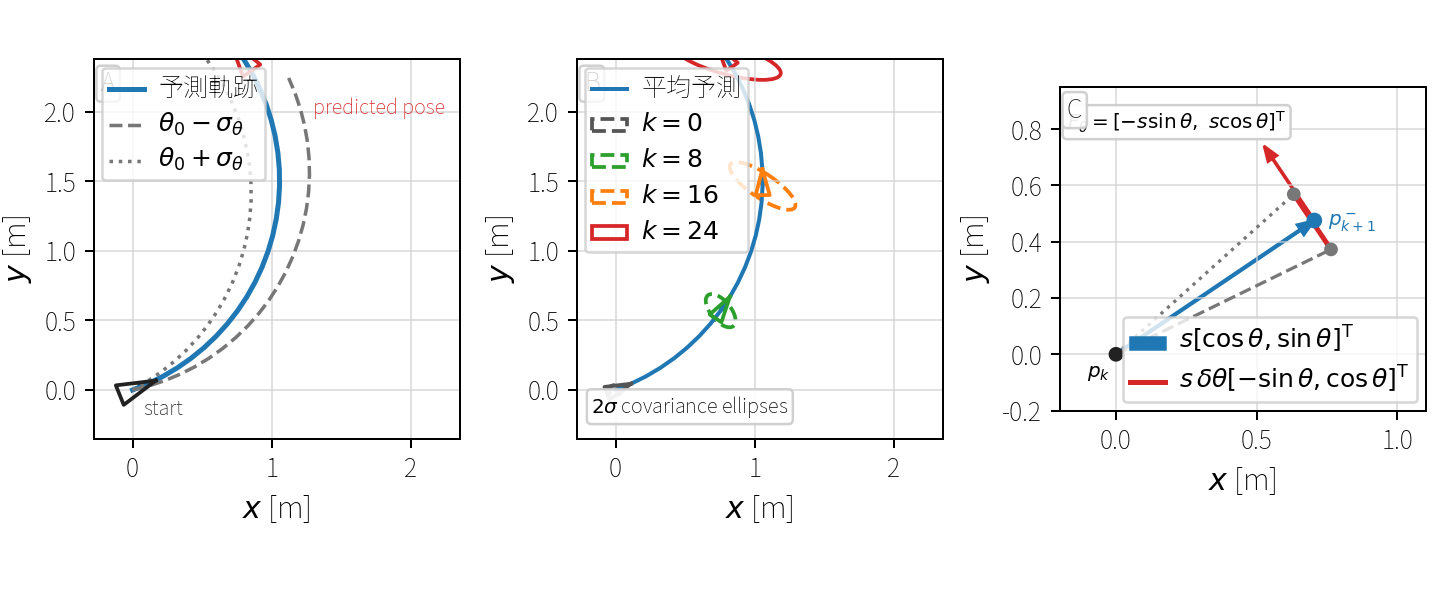
\includegraphics[width=0.96\linewidth,bb=0 0 1440 603]{figures/flow6_kalman_pose_bridge_examples.png}
\caption{線形 Kalman フィルタの共分散予測を差動二輪の非線形姿勢予測へ接続する幾何。左はオドメトリによる円弧状の平均姿勢予測と初期方位のずれによる終点差、中央は局所ヤコビアンで伝搬した $2\sigma$ 共分散楕円、右は $F_k$ の方位列が前進距離に比例した横方向感度を表すことを示している。}
\label{fig:kalman-pose-bridge-examples}
\end{figure}

ここまでで、相補フィルタの固定重みでは扱いにくかったセンサ融合の失敗は、$P^-$、革新、Kalman ゲインという線形 Kalman フィルタの二段構造で読み替えられることが分かる。同時に、ロボットの姿勢予測そのものは $\sin\theta$ と $\cos\theta$ を含むため、固定行列の線形モデルには戻らない。残る手順は、時々刻々の予測点で $F_k$ を作り、測定式も必要なら同じように局所線形化して、線形 Kalman フィルタの予測と更新の形へ入れることである。この手順が、次に扱う拡張 Kalman フィルタの出発点になる。

\subsection{EKF}

前節では、差動二輪ロボットのオドメトリ予測で、向きの不確かさが走行距離に比例して横方向の位置共分散へ伸びることを見た。相補フィルタの固定重みでは、車輪すべり、ジャイロバイアス、外部測定の粗さを時々刻々で区別しにくい。一方、線形 Kalman フィルタの予測共分散、革新、Kalman ゲインは、その区別を数量として持てる。ただし姿勢予測そのものは $\sin\theta$ と $\cos\theta$ を含むため、固定行列 $A,C$ だけでは表せない。したがって次に必要になるのは、平均は非線形なロボット運動学で進め、共分散と革新だけを現在の推定値の近くで線形化する手順である。

線形カルマンフィルタは、線形モデル $A,C$ と共分散 $Q,R$ を使って予測と更新を行った。拡張 Kalman フィルタは、この二段構造を保ったまま、状態遷移と測定の式を非線形写像へ広げる方法である。離散時間の非線形確率モデルを
\begin{align}
  x_k&=f_{k-1}(x_{k-1},u_{k-1})+G_{k-1}w_{k-1},\\
  y_k&=h_k(x_k)+v_k
\end{align}
とする。状態は $x_k\in\R^n$、入力は $u_k\in\R^m$、測定は $y_k\in\R^p$ である。$w_k$ はプロセスノイズ、$v_k$ は測定ノイズであり、
\begin{align}
  E[w_i]&=0,
  &E[v_i]&=0,\\
  E[w_iw_j^\T]&=Q_{w,i}\delta_{ij},
  &E[v_iv_j^\T]&=R_{v,i}\delta_{ij},\\
  E[w_iv_j^\T]&=0
\end{align}
を仮定する。ここで $Q_{w,k}$ は半正定値、$R_{v,k}$ は正定値である。線形カルマンフィルタでは $f(x,u)=Ax+Bu$、$h(x)=Cx$ であった。EKF では、平均値そのものは非線形写像で進め、誤差共分散だけを現在の推定値まわりの一次近似で進める。

予測平均は
\begin{equation}
  \hat{x}_{k|k-1}
  =f_{k-1}(\hat{x}_{k-1|k-1},u_{k-1})
\end{equation}
で与える。状態遷移のヤコビアンを
\begin{equation}
  F_{k-1}
  =
  \left.\frac{\pp f_{k-1}}{\pp x}\right|_{(\hat{x}_{k-1|k-1},u_{k-1})}
\end{equation}
と定義すると、予測誤差 $e_{k|k-1}=x_k-\hat{x}_{k|k-1}$ は一次近似で
\begin{align}
  e_{k|k-1}
  &=f_{k-1}(\hat{x}_{k-1|k-1}+e_{k-1|k-1},u_{k-1})
    -f_{k-1}(\hat{x}_{k-1|k-1},u_{k-1})
    +G_{k-1}w_{k-1}\\
  &\simeq F_{k-1}e_{k-1|k-1}+G_{k-1}w_{k-1}
\end{align}
となる。したがって、交差共分散が 0 であるという仮定から
\begin{equation}
  P_{k|k-1}
  =
  F_{k-1}P_{k-1|k-1}F_{k-1}^\T
  +G_{k-1}Q_{w,k-1}G_{k-1}^\T
\end{equation}
を得る。プロセスノイズが加法的でなく
\begin{equation}
  x_k=f_{k-1}(x_{k-1},u_{k-1},w_{k-1})
\end{equation}
の形で入る場合は、ノイズのヤコビアン
\begin{equation}
  W_{k-1}
  =
  \left.\frac{\pp f_{k-1}}{\pp w}\right|_{(\hat{x}_{k-1|k-1},u_{k-1},0)}
\end{equation}
を用い、上式の $G_{k-1}Q_{w,k-1}G_{k-1}^\T$ を $W_{k-1}Q_{w,k-1}W_{k-1}^\T$ に置き換える。

測定更新では、まず予測測定値を
\begin{equation}
  \hat{y}_{k|k-1}=h_k(\hat{x}_{k|k-1})
\end{equation}
と置き、革新を
\begin{equation}
  \nu_k=y_k-\hat{y}_{k|k-1}
\end{equation}
と定義する。測定写像のヤコビアンは予測状態のまわりで
\begin{equation}
  H_k=
  \left.\frac{\pp h_k}{\pp x}\right|_{\hat{x}_{k|k-1}}
\end{equation}
である。測定式を一次近似すると
\begin{align}
  \nu_k
  &=h_k(x_k)+v_k-h_k(\hat{x}_{k|k-1})\\
  &\simeq H_ke_{k|k-1}+v_k
\end{align}
であるから、革新共分散と Kalman ゲインは
\begin{align}
  S_k&=H_kP_{k|k-1}H_k^\T+R_{v,k},\\
  K_k&=P_{k|k-1}H_k^\T S_k^{-1}
\end{align}
となる。更新後の推定値と共分散は
\begin{align}
  \hat{x}_{k|k}
  &=\hat{x}_{k|k-1}+K_k\nu_k,\\
  P_{k|k}
  &=(I-K_kH_k)P_{k|k-1}(I-K_kH_k)^\T
    +K_kR_{v,k}K_k^\T
\end{align}
である。最後の式は Joseph 形式であり、線形カルマンフィルタと同じ理由で、有限精度計算における対称性と半正定値性を保ちやすい。

\begin{derivation}
EKF の共分散式は、線形カルマンフィルタの式に見た目だけ似せたものではない。状態遷移のテイラー展開
\begin{equation}
  f(\hat{x}+e,u)
  =
  f(\hat{x},u)
  +F e
  +\text{二次以上の項}
\end{equation}
で二次以上の項を無視すると、誤差は $e^-\simeq Fe+Gw$ に従う。したがって
\begin{align}
  P^-
  &=E[e^-(e^-)^\T]\\
  &\simeq E[(Fe+Gw)(Fe+Gw)^\T]\\
  &=F E[ee^\T]F^\T+G E[ww^\T]G^\T
\end{align}
となる。測定側でも $h(\hat{x}^-+e^-)\simeq h(\hat{x}^-)+He^-$ なので、革新は $\nu\simeq He^-+v$ である。この局所線形な革新モデルに対して、線形カルマンフィルタと同じ平均二乗誤差最小化を行うと $K=P^-H^\T(HP^-H^\T+R)^{-1}$ が得られる。
\end{derivation}

$f_{k-1}(x,u)=A_{k-1}x+B_{k-1}u$、$h_k(x)=C_kx$ の場合、ヤコビアンは常に $F_{k-1}=A_{k-1}$、$H_k=C_k$ である。このとき予測平均、共分散、革新、ゲイン、更新の全式は離散時間 Kalman フィルタそのものに戻る。したがって EKF は、線形 Kalman フィルタと別の原理で作られた推定器ではなく、線形 Kalman フィルタを時々刻々の接線モデルへ適用する非線形拡張である。

この解釈は、EKF の限界も同時に示す。一般には $E[f(x)]\ne f(E[x])$ であるため、予測平均を $f(\hat{x})$ で進める操作は厳密な条件付き平均ではない。さらに、共分散は一次テイラー展開に基づくので、推定誤差が大きい、初期値が悪い、測定関数が強く曲がる、ヤコビアンが特異に近い、ノイズが強い非ガウス性を持つ、または角度や姿勢のように状態空間が普通のベクトル空間でない場合には、単一の正規分布と接線モデルだけでは不確かさを十分に表せない。EKF を使うときは、線形化点、サンプリング周期、ノイズ共分散、測定の可観測性を一つの設計条件として確認する必要がある。

\begin{example}[二乗測定をもつスカラー系]
状態がゆっくり変化するスカラー系
\begin{align}
  x_k&=x_{k-1}+w_{k-1},\\
  y_k&=x_k^2+v_k
\end{align}
を考える。状態遷移は線形なので $F_{k-1}=1$、測定写像は $h(x)=x^2$ なので
\begin{equation}
  H_k=\left.\frac{\dd}{\dd x}x^2\right|_{\hat{x}_{k|k-1}}
  =2\hat{x}_{k|k-1}
\end{equation}
である。予測は
\begin{align}
  \hat{x}_{k|k-1}&=\hat{x}_{k-1|k-1},\\
  P_{k|k-1}&=P_{k-1|k-1}+Q_{w,k-1}
\end{align}
となり、革新とゲインは
\begin{align}
  \nu_k&=y_k-\hat{x}_{k|k-1}^2,\\
  S_k&=4\hat{x}_{k|k-1}^2P_{k|k-1}+R_{v,k},\\
  K_k&=\frac{2P_{k|k-1}\hat{x}_{k|k-1}}{S_k}
\end{align}
である。予測値が正で、実測 $y_k$ が予測された二乗値より大きければ、革新は正でゲインも正なので推定値は正方向へ修正される。予測値が負ならゲインの符号も負になり、同じ正の革新は推定値をより負の方向へ修正する。これは、$x^2$ の曲線を現在の予測点で接線近似しているためである。

一方、$\hat{x}_{k|k-1}$ が 0 に近いと $H_k\simeq0$ となり、$K_k$ も小さくなる。測定 $y_k=x_k^2+v_k$ は状態の大きさに関する情報を持つが、符号を区別しない。単一の接線と単一の正規分布で表す EKF は、この大域的な二峰性を表せない。したがって、この例では「非線形測定を線形化して使う」という利点と、「線形化点の周辺でしか情報を正しく読めない」という限界が同時に現れる。
\end{example}

\begin{example}[差動二輪ロボットの外部位置測定による EKF 更新]
オドメトリだけで進む差動二輪ロボットでは、車輪すべりやジャイロバイアスによって経路全体が少しずつ横へずれる。ここに、天井カメラ、測位マーカ、またはランドマーク照合から得られる外部位置測定を時々入れると、非線形予測と線形 Kalman 更新の役割を具体的に見られる。状態を
\begin{equation}
  x_k=
  \begin{bmatrix}
    p_{x,k}\\p_{y,k}\\\theta_k
  \end{bmatrix}
\end{equation}
とし、サンプリング間の走行距離を $\Delta s_k$、向きの変化を $\Delta\theta_k$ とする。予測は、前節のオドメトリと同じく
\begin{align}
  \hat{p}_{x,k|k-1}
  &=
  \hat{p}_{x,k-1|k-1}
  +\Delta s_k\cos\psi_k,\\
  \hat{p}_{y,k|k-1}
  &=
  \hat{p}_{y,k-1|k-1}
  +\Delta s_k\sin\psi_k,\\
  \hat{\theta}_{k|k-1}
  &=
  \hat{\theta}_{k-1|k-1}+\Delta\theta_k,
  \qquad
  \psi_k=\hat{\theta}_{k-1|k-1}+\frac{\Delta\theta_k}{2}
\end{align}
で進める。この式は $\cos\psi_k,\sin\psi_k$ を含むので、平均値は非線形に伝搬する。一方、姿勢誤差が位置誤差へどう移るかは、現在の予測点のヤコビアン
\begin{equation}
  F_k
  =
  \begin{bmatrix}
    1&0&-\Delta s_k\sin\psi_k\\
    0&1& \Delta s_k\cos\psi_k\\
    0&0&1
  \end{bmatrix}
\end{equation}
で共分散へ入る。たとえば前向きに長く走るほど、第三列の大きさが増え、向きの不確かさが横方向の位置不確かさへ写る。

外部測定が位置だけを返す場合を
\begin{equation}
  y_k=
  \begin{bmatrix}
    z_{x,k}\\z_{y,k}
  \end{bmatrix}
  =
  h(x_k)+v_k,
  \qquad
  h(x_k)=
  \begin{bmatrix}
    p_{x,k}\\p_{y,k}
  \end{bmatrix},
  \qquad
  R_k=\sigma_z^2 I
\end{equation}
と書く。予測測定と革新は
\begin{equation}
  \hat{y}_{k|k-1}=
  \begin{bmatrix}
    \hat{p}_{x,k|k-1}\\
    \hat{p}_{y,k|k-1}
  \end{bmatrix},
  \qquad
  \nu_k=
  \begin{bmatrix}
    z_{x,k}-\hat{p}_{x,k|k-1}\\
    z_{y,k}-\hat{p}_{y,k|k-1}
  \end{bmatrix}
\end{equation}
であり、測定ヤコビアンは
\begin{equation}
  H_k=
  \begin{bmatrix}
    1&0&0\\
    0&1&0
  \end{bmatrix}
\end{equation}
である。したがって革新共分散とゲインは
\begin{align}
  S_k
  &=
  H_kP_{k|k-1}H_k^\T+\sigma_z^2I,\\
  K_k
  &=
  P_{k|k-1}H_k^\T S_k^{-1}
  =
  \begin{bmatrix}
    P^-_{xx}&P^-_{xy}\\
    P^-_{yx}&P^-_{yy}\\
    P^-_{\theta x}&P^-_{\theta y}
  \end{bmatrix}
  S_k^{-1}
\end{align}
となる。ここで $P^-_{ij}$ は $P_{k|k-1}$ の成分である。更新は
\begin{align}
  \hat{x}_{k|k}
  &=
  \hat{x}_{k|k-1}+K_k\nu_k,\\
  P_{k|k}
  &=
  (I-K_kH_k)P_{k|k-1}(I-K_kH_k)^\T
  +K_kR_kK_k^\T
\end{align}
である。位置しか測っていなくても、第三行に $P^-_{\theta x},P^-_{\theta y}$ が入るため、予測で生じた位置と向きの相関を通して姿勢も補正される。これは「位置測定から突然角度を測った」わけではなく、非線形オドメトリが作った共分散の傾きを使って、位置ずれを最も起こしやすい向き誤差へ戻しているという解釈である。

測定の信頼度を変えると補正の大きさも変わる。たとえば $x$ 方向だけを見て $P^-_{xx}=0.20^2\,\mathrm{m}^2$ とすると、測定標準偏差が $\sigma_z=0.05\,\mathrm{m}$ のとき
\begin{equation}
  \frac{P^-_{xx}}{P^-_{xx}+\sigma_z^2}
  =
  \frac{0.04}{0.04+0.0025}
  \simeq0.94
\end{equation}
であり、外部測定に近い位置へ強く寄る。測定標準偏差が $\sigma_z=0.50\,\mathrm{m}$ なら
\begin{equation}
  \frac{0.04}{0.04+0.25}
  \simeq0.14
\end{equation}
となり、更新は主にオドメトリ予測を保つ。反対に、すべりを疑ってプロセスノイズを大きくし、$P_{k|k-1}$ を膨らませると、同じ測定でも $K_k$ は大きくなる。したがって $Q$ は「どれだけ予測を疑うか」、$R$ は「どれだけ測定を疑うか」を決める設計量であり、革新 $\nu_k$ が大きすぎるときは $\nu_k^\T S_k^{-1}\nu_k$ を見て外れ値や線形化の破れを疑う。
\end{example}

\subsection{ESKF}

誤差状態 Kalman フィルタ（error-state Kalman filter; ESKF）は、状態そのものを線形化した座標で持つのではなく、非線形な名目状態と、その近くの小さな誤差状態を分けて扱う EKF である。姿勢を四元数 $q$ または回転行列 $R\in\SO(3)$ で表す場合、$q$ には $\norm{q}=1$、$R$ には $R^\T R=I$ と $\det R=1$ という制約がある。通常の EKF のように四元数の 4 成分へ補正量を直接足すと、この制約から外れやすい。足した後に四元数を正規化しても、補正の一部は単位球面の半径方向へ消え、共分散には物理的な姿勢誤差ではない 4 成分目の広がりが残りうる。さらに、補正後の名目姿勢が変わると、その近くの接平面も変わるため、古い座標で持った共分散をそのまま次の時刻へ使うと、局所誤差の意味がずれやすい。ESKF では、姿勢本体は曲面上の名目状態として積分し、共分散は小角度誤差 $\delta\theta\in\R^3$ のような最小座標に持たせる。測定更新で得た小さい誤差を名目状態へ注入し、その直後に誤差平均を 0 へ戻すことで、共分散を常に現在の名目姿勢の接空間に置き直す。

図\ref{fig:flow6-eskf-structure}は、この分離を信号経路として表したものである。IMU 測定は上段の名目状態を多様体上で非線形に伝搬し、同じ測定から下段の誤差状態モデルと共分散伝搬も決まる。外部測定が入ると、名目状態から予測測定を作って革新を計算し、その革新で接空間上の誤差状態を更新する。得られた $\widehat{\delta x}$ は名目状態へ注入され、誤差平均は 0 にリセットされる。この流れにより、姿勢本体は常に $\SO(3)$ または単位四元数上に残り、共分散は名目姿勢の近くの小さい誤差だけを表し続ける。

\begin{figure}[tb]
\centering
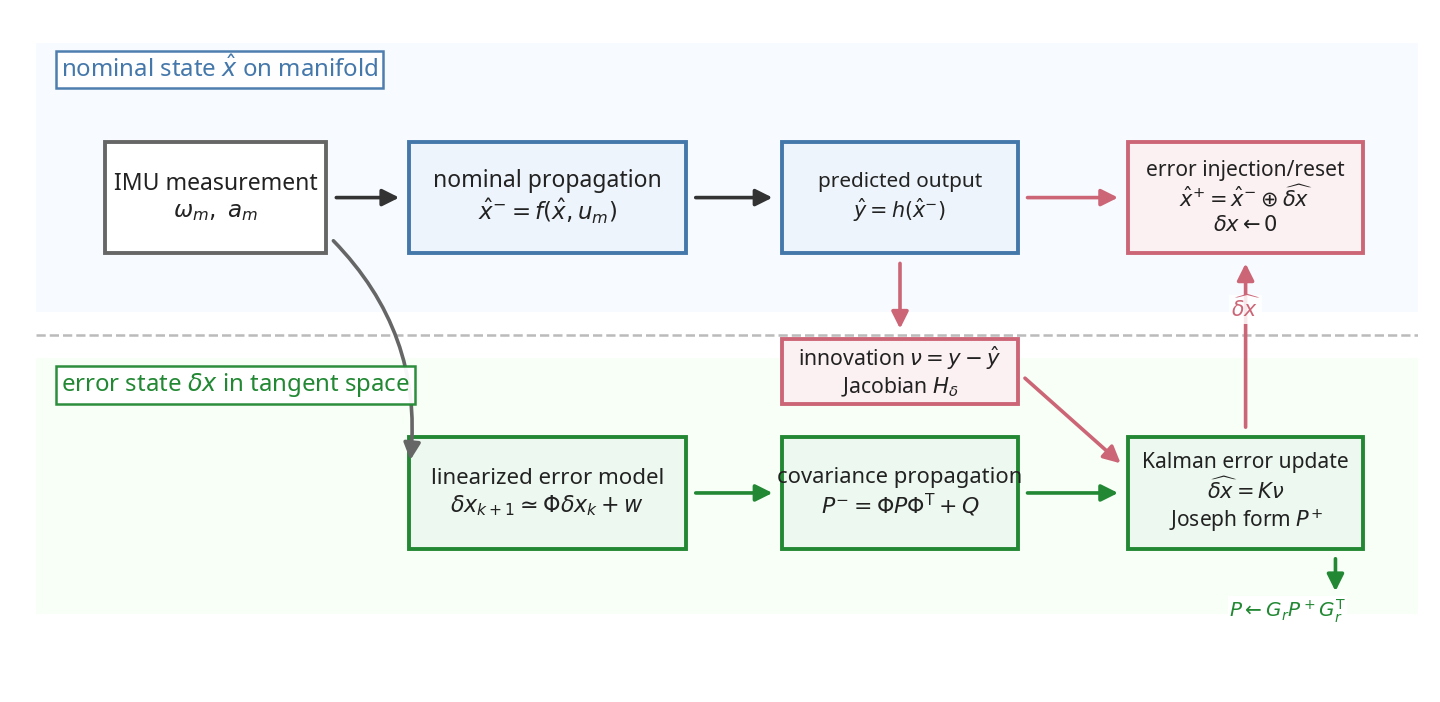
\includegraphics[width=0.96\linewidth,bb=0 0 1440 702]{figures/flow6_eskf_structure.png}
\caption{ESKF における名目状態と誤差状態の分離。IMU 測定は名目状態を伝搬し、同時に接空間上の誤差共分散を伝搬する。測定革新は誤差状態を更新し、推定された誤差は名目状態へ注入されてからリセットされる。}
\label{fig:flow6-eskf-structure}
\end{figure}

\subsubsection{名目状態と誤差状態の分離}

IMU を用いる剛体の推定では、名目状態を
\begin{equation}
  \hat{x}
  =
  \left(
    \hat{p}^I,\hat{v}^I,\hat{q}^I_B,
    \hat{b}_g,\hat{b}_a
  \right)
\end{equation}
のように選ぶことが多い。ここで $\hat{p}^I$ [m] は慣性座標系で表した位置、$\hat{v}^I$ [m/s] は速度、$\hat{q}^I_B$ は機体系 $\{B\}$ から慣性系 $\{I\}$ への姿勢を表す単位四元数、$\hat{b}_g$ [rad/s] はジャイロバイアス、$\hat{b}_a$ [m/s$^2$] は加速度計バイアスである。位置や速度を推定しない姿勢推定では、$p^I,v^I$ を除いた小さい名目状態を使ってもよい。

この名目状態に対応する誤差状態を
\begin{equation}
  \delta x
  =
  \begin{bmatrix}
    \delta p^I\\
    \delta v^I\\
    \delta\theta\\
    \delta b_g\\
    \delta b_a
  \end{bmatrix}
  \in\R^{15}
\end{equation}
と置く。以下で使う $[r]_\times$ は、任意の $s\in\R^3$ に対して $[r]_\times s=r\times s$ を満たす歪対称行列である。真の状態と名目状態の関係は
\begin{align}
  p^I&=\hat{p}^I+\delta p^I,\\
  v^I&=\hat{v}^I+\delta v^I,\\
  q^I_B&=\hat{q}^I_B\otimes\delta q(\delta\theta),\\
  b_g&=\hat{b}_g+\delta b_g,\\
  b_a&=\hat{b}_a+\delta b_a
\end{align}
である。右から掛ける $\delta q(\delta\theta)$ は、名目姿勢から真の姿勢へ戻す小回転を機体系側で表す。小角度では
\begin{equation}
  \delta q(\delta\theta)
  \simeq
  \begin{bmatrix}
    1\\
    \delta\theta/2
  \end{bmatrix}
\end{equation}
であり、回転行列で書けば
\begin{equation}
  R^I_B=\hat{R}^I_B\operatorname{Exp}([\delta\theta]_\times)
  \simeq
  \hat{R}^I_B(I+[\delta\theta]_\times)
\end{equation}
である。したがって、フィルタが持つ共分散 $P$ は四元数 4 成分の共分散ではなく、$\delta p^I,\delta v^I,\delta\theta,\delta b_g,\delta b_a$ に関する共分散である。

IMU の測定モデルを
\begin{align}
  \omega_m&=\omega^B+b_g+n_g,\\
  a_m&=f^B+b_a+n_a
\end{align}
とする。$\omega_m$ [rad/s] はジャイロ測定、$a_m$ [m/s$^2$] は加速度計測定、$\omega^B$ は機体系角速度、$f^B$ は機体系で表した比力である。$n_g,n_a$ は平均 0 の白色ノイズであり、バイアスはゆっくり変わるランダムウォークとして
\begin{align}
  \dot{b}_g&=n_{bg},\\
  \dot{b}_a&=n_{ba}
\end{align}
で表す。比力 $f^B$ は重力を除いた加速度であり、慣性系の重力加速度を $g^I$ とすると並進運動は
\begin{equation}
  \dot{v}^I=R^I_B f^B+g^I
\end{equation}
である。

\subsubsection{連続時間の名目伝搬と誤差伝搬}

名目状態は、IMU 測定からバイアス推定値を引いた
\begin{equation}
  \hat{\omega}=\omega_m-\hat{b}_g,
  \qquad
  \hat{a}=a_m-\hat{b}_a
\end{equation}
を使って非線形に伝搬する。連続時間では
\begin{align}
  \dot{\hat{p}}^I&=\hat{v}^I,\\
  \dot{\hat{v}}^I&=\hat{R}^I_B\hat{a}+g^I,\\
  \dot{\hat{q}}^I_B
  &=
  \frac{1}{2}\hat{q}^I_B\otimes
  \begin{bmatrix}
    0\\ \hat{\omega}
  \end{bmatrix},\\
  \dot{\hat{b}}_g&=0,\\
  \dot{\hat{b}}_a&=0
\end{align}
と書く。数値積分では四元数を随時正規化し、$\norm{\hat{q}^I_B}=1$ を保つ。ここで非線形な姿勢積分そのものを線形モデルへ置き換えているわけではない。線形化するのは、名目状態のまわりの小さな誤差の運動である。

右乗法誤差
\begin{equation}
  R^I_B=\hat{R}^I_B\operatorname{Exp}([\delta\theta]_\times)
\end{equation}
を用い、二次以上の小さい項を無視すると、誤差状態は
\begin{equation}
  \delta\dot{x}
  =
  F_c\delta x+G_cn
\end{equation}
に従う。ただし
\begin{equation}
  n=
  \begin{bmatrix}
    n_g\\ n_a\\ n_{bg}\\ n_{ba}
  \end{bmatrix}
\end{equation}
であり、
\begin{equation}
  F_c=
  \begin{bmatrix}
    0&I&0&0&0\\
    0&0&-\hat{R}^I_B[\hat{a}]_\times&0&-\hat{R}^I_B\\
    0&0&-[\hat{\omega}]_\times&-I&0\\
    0&0&0&0&0\\
    0&0&0&0&0
  \end{bmatrix},
  \qquad
  G_c=
  \begin{bmatrix}
    0&0&0&0\\
    0&-\hat{R}^I_B&0&0\\
    -I&0&0&0\\
    0&0&I&0\\
    0&0&0&I
  \end{bmatrix}.
\end{equation}
第二行の $-\hat{R}^I_B[\hat{a}]_\times\delta\theta$ は、姿勢誤差が比力の慣性系成分を変えることを表す。第三行の $-[\hat{\omega}]_\times\delta\theta-\delta b_g$ は、角速度の名目値まわりで姿勢誤差が回転し、ジャイロバイアス誤差が角度誤差として蓄積することを表す。

\begin{derivation}
速度誤差の主要項は、真の並進式と名目並進式の差から得られる。$a_m-b_a-n_a=\hat{a}-\delta b_a-n_a$ と $R^I_B\simeq\hat{R}^I_B(I+[\delta\theta]_\times)$ を使うと
\begin{align}
  \delta\dot{v}^I
  &=
  R^I_B(a_m-b_a-n_a)-\hat{R}^I_B\hat{a}\\
  &\simeq
  \hat{R}^I_B(I+[\delta\theta]_\times)
  (\hat{a}-\delta b_a-n_a)
  -\hat{R}^I_B\hat{a}\\
  &\simeq
  \hat{R}^I_B[\delta\theta]_\times\hat{a}
  -\hat{R}^I_B\delta b_a
  -\hat{R}^I_B n_a\\
  &=
  -\hat{R}^I_B[\hat{a}]_\times\delta\theta
  -\hat{R}^I_B\delta b_a
  -\hat{R}^I_B n_a .
\end{align}
同様に、姿勢の右誤差を一次まで残すと
\begin{equation}
  \delta\dot{\theta}
  \simeq
  -[\hat{\omega}]_\times\delta\theta-\delta b_g-n_g
\end{equation}
となる。
\end{derivation}

\subsubsection{離散時間予測と共分散伝搬}

サンプリング周期を $\Delta t$ とする。もっとも単純な一段の離散化では、名目状態を
\begin{align}
  \hat{p}^I_{k+1}
  &=
  \hat{p}^I_k+\hat{v}^I_k\Delta t
  +\frac{1}{2}(\hat{R}^I_{B,k}\hat{a}_k+g^I)\Delta t^2,\\
  \hat{v}^I_{k+1}
  &=
  \hat{v}^I_k+(\hat{R}^I_{B,k}\hat{a}_k+g^I)\Delta t,\\
  \hat{q}^I_{B,k+1}
  &=
  \hat{q}^I_{B,k}\otimes\delta q(\hat{\omega}_k\Delta t),\\
  \hat{b}_{g,k+1}&=\hat{b}_{g,k},\\
  \hat{b}_{a,k+1}&=\hat{b}_{a,k}
\end{align}
で進める。実装では、姿勢更新後に
\begin{equation}
  \hat{q}^I_{B,k+1}
  \leftarrow
  \frac{\hat{q}^I_{B,k+1}}{\norm{\hat{q}^I_{B,k+1}}}
\end{equation}
と正規化する。高精度が必要なら、中点法や Runge--Kutta 法で名目状態を積分し、同じ区間で誤差遷移行列も積分する。

誤差状態の離散近似は
\begin{equation}
  \delta x_{k+1}
  \simeq
  \Phi_k\delta x_k+w_{\delta,k}
\end{equation}
であり、一次近似では
\begin{equation}
  \Phi_k\simeq I+F_{c,k}\Delta t
\end{equation}
である。連続時間白色ノイズの共分散密度を
\begin{equation}
  E[n(t)n(\tau)^\T]=Q_c\delta(t-\tau)
\end{equation}
で定義すると、離散時間のプロセスノイズ共分散は
\begin{equation}
  Q_{d,k}
  =
  \int_0^{\Delta t}
  \Phi(\Delta t-\tau)G_cQ_cG_c^\T
  \Phi(\Delta t-\tau)^\T\,\dd\tau
\end{equation}
で定義される。短い周期では
\begin{equation}
  Q_{d,k}\simeq G_{c,k}Q_cG_{c,k}^\T\Delta t
\end{equation}
を用いることが多い。したがって共分散予測は
\begin{equation}
  P_{k+1|k}
  =
  \Phi_kP_{k|k}\Phi_k^\T+Q_{d,k}
\end{equation}
である。

\subsubsection{測定更新と誤差注入}

位置、速度、姿勢、重力方向、磁気方位、距離などの測定をまとめて
\begin{equation}
  y_k=h(\hat{x}_{k|k-1}\oplus\delta x_k)+v_k
\end{equation}
と書く。記号 $\oplus$ は、ユークリッド成分には足し算、姿勢成分には小回転の乗法を使って誤差を名目状態へ載せる操作を表す。測定の予測値と革新を
\begin{equation}
  \hat{y}_{k|k-1}=h(\hat{x}_{k|k-1}),
  \qquad
  \nu_k=y_k-\hat{y}_{k|k-1}
\end{equation}
と置き、誤差状態に関する測定ヤコビアンを
\begin{equation}
  H_{\delta,k}
  =
  \left.
  \frac{\pp h(\hat{x}_{k|k-1}\oplus\delta x)}
       {\pp\delta x}
  \right|_{\delta x=0}
\end{equation}
で定義する。一次近似では
\begin{equation}
  \nu_k\simeq H_{\delta,k}\delta x_k+v_k
\end{equation}
となるので、通常の Kalman 型更新として
\begin{align}
  S_k&=H_{\delta,k}P_{k|k-1}H_{\delta,k}^\T+R_k,\\
  K_k&=P_{k|k-1}H_{\delta,k}^\T S_k^{-1},\\
  \widehat{\delta x}_k&=K_k\nu_k,\\
  P^+_k
  &=(I-K_kH_{\delta,k})P_{k|k-1}
    (I-K_kH_{\delta,k})^\T+K_kR_kK_k^\T
\end{align}
を計算する。ここで $\widehat{\delta x}_k$ は、真の誤差状態の推定値である。

更新後は、推定された誤差を名目状態へ注入し、誤差状態の平均を 0 に戻す。すなわち
\begin{align}
  \hat{p}^{I,+}&=\hat{p}^{I,-}+\widehat{\delta p}^I,\\
  \hat{v}^{I,+}&=\hat{v}^{I,-}+\widehat{\delta v}^I,\\
  \hat{q}^{I,+}_B
  &=
  \hat{q}^{I,-}_B\otimes
  \delta q(\widehat{\delta\theta}),\\
  \hat{b}^+_g&=\hat{b}^-_g+\widehat{\delta b}_g,\\
  \hat{b}^+_a&=\hat{b}^-_a+\widehat{\delta b}_a
\end{align}
とし、四元数を正規化する。続いて
\begin{equation}
  \delta x\leftarrow0
\end{equation}
とリセットする。このリセットは平均だけでなく共分散にも影響する。注入前の誤差から注入後の誤差への一次変換を $G_r$ とすれば
\begin{equation}
  P_{k|k}=G_rP^+_kG_r^\T
\end{equation}
である。右乗法の小さい姿勢補正では、姿勢ブロックに
\begin{equation}
  G_{r,\theta\theta}
  \simeq
  I-\frac{1}{2}[\widehat{\delta\theta}]_\times
\end{equation}
を使うことが多い。補正角が十分小さい場合は $G_r\simeq I$ としても大きな差は出にくいが、大きな革新を頻繁に注入する実装では、リセットヤコビアンを省くと共分散の整合性が悪くなる。

\subsubsection{ESKF の数値トレース}

式だけでは、名目姿勢と誤差状態を分ける利点を数量として追いにくい。ここでは、ピッチ角だけを取り出した 1 次元の姿勢更新で、IMU 予測、共分散、革新、注入、リセットを数値で追う。ジャイロ積分だけで進む名目角は、未補償のジャイロバイアスによって少しずつ真値から離れる。一方、加速度計から得る傾きは重力方向を使うため低速時にはロールとピッチを拘束できるが、並進加速度が混ざると重力方向そのものからずれる。この二つの限界を、ESKF は「予測をどれだけ疑うか」を $P^-_{\theta,k}$、「加速度計の傾きをどれだけ信じるか」を $R_{\theta,k}$ として分けて扱う。

数値例では、時刻 $t=4.0\,\mathrm{s}$ で真のピッチ角が $0.55^\circ$、ジャイロ積分で得た名目予測が $1.56^\circ$、加速度計から作った傾き測定が $-0.20^\circ$ であったとする。このとき革新は
\begin{equation}
  \nu_{\theta,k}
  =
  y_{\theta,k}-\hat{\theta}^{-}_k
  =
  -1.76^\circ
\end{equation}
であり、更新直前の姿勢標準偏差は $\sqrt{P^-_{\theta,k}}=1.52^\circ$ まで増えている。ピッチだけに限定すると、誤差状態の測定モデルは
\begin{equation}
  \nu_{\theta,k}
  \simeq
  \delta\theta_k+v_{\theta,k}
\end{equation}
なので
\begin{align}
  S_{\theta,k}&=P^-_{\theta,k}+R_{\theta,k},\\
  K_{\theta,k}&=P^-_{\theta,k}S_{\theta,k}^{-1},\\
  \widehat{\delta\theta}_k&=K_{\theta,k}\nu_{\theta,k},\\
  P^+_{\theta,k}
  &=(1-K_{\theta,k})^2P^-_{\theta,k}
    +K_{\theta,k}^2R_{\theta,k}
\end{align}
で更新できる。たとえば加速度計の傾き標準偏差を $1.20^\circ$ と仮定する標準設定では、$K_{\theta,k}=0.62$、$\widehat{\delta\theta}_k=-1.09^\circ$、$\sqrt{P^+_{\theta,k}}=0.94^\circ$ となる。この小角度を名目姿勢へ
\begin{equation}
  \hat{q}^{+}
  =
  \hat{q}^{-}\otimes\delta q(\widehat{\delta\theta}_k)
\end{equation}
として注入し、直後に誤差平均を
\begin{equation}
  \delta\theta\leftarrow0
\end{equation}
へ戻す。今回の 1 次元トレースでは補正角が小さいため $G_{r,\theta\theta}\simeq1$ と近似し、共分散はほぼ $P^+_{\theta,k}$ のまま現在の名目姿勢まわりの誤差幅として読み替えられる。

\begin{figure}[tb]
\centering
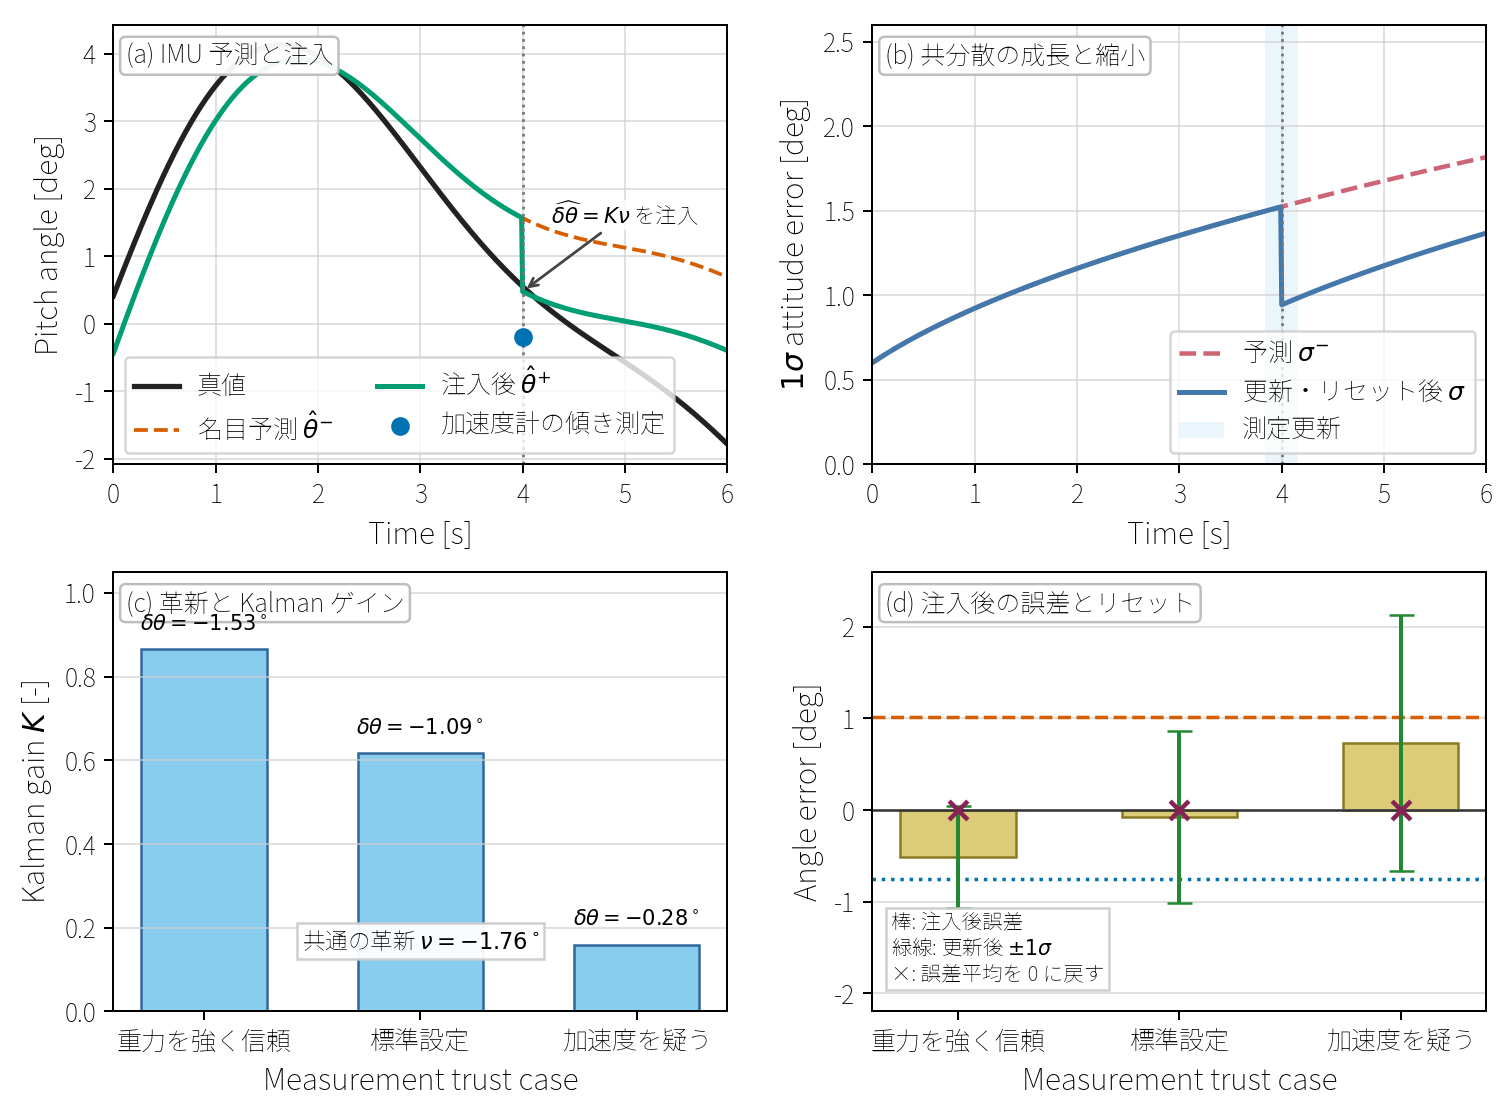
\includegraphics[width=0.98\linewidth,bb=0 0 1512 1116]{figures/flow6_eskf_numeric_trace.png}
\caption{ESKF の 1 次元姿勢更新トレース。ジャイロ積分で名目姿勢がドリフトし、同時に姿勢共分散が増える。加速度計から得た傾き測定の革新で小角度誤差 $\widehat{\delta\theta}$ を推定し、名目姿勢へ注入してから誤差平均を 0 へリセットする。測定を強く信頼すると加速度外乱にも寄りやすく、測定を疑うとジャイロドリフトが残りやすい。}
\label{fig:flow6-eskf-numeric-trace}
\end{figure}

図\ref{fig:flow6-eskf-numeric-trace}では、上段左に真値、ジャイロ積分だけの名目予測、注入後の名目姿勢を重ねている。上段右では、更新前の標準偏差が時間とともに増え、測定更新で小さくなった後、再びジャイロノイズとバイアス不確かさで増える。下段左は測定信頼度を変えたときの Kalman ゲインであり、加速度計を強く信頼する $0.60^\circ$ 設定では $K=0.87$、標準設定では $K=0.62$、急加速中として疑う $3.50^\circ$ 設定では $K=0.16$ になる。同じ革新 $-1.76^\circ$ でも、注入する局所姿勢誤差はそれぞれ $-1.53^\circ$、$-1.09^\circ$、$-0.28^\circ$ に変わる。

下段右は、この重み付けが破綻モードの解釈を決めることを示している。加速度計を強く信頼すると、ジャイロドリフトによる $1.01^\circ$ の予測誤差は大きく消えるが、加速度計の傾きに $-0.75^\circ$ の非重力加速度成分が混ざっていると、その外乱にも引かれる。反対に加速度計を強く疑うと、外乱には引かれにくいが、更新後も正の姿勢誤差が残る。したがって、静止または低加速度で重力方向が信頼できる時刻は $R_{\theta,k}$ を小さくでき、急加速、振動、衝突、センサ飽和が疑われる時刻は $R_{\theta,k}$ を大きくするか革新を棄却する必要がある。重力方向だけではヨー角を拘束できないため、ヨーのジャイロドリフトには磁気方位、外部姿勢、位置変化から得た方位情報など、別の測定が必要になる。

\subsubsection{EKF との関係と適用条件}

ESKF は EKF と別のベイズ更新を使う方法ではない。予測、革新、Kalman ゲイン、Joseph 形式の共分散更新は EKF と同じであり、違いは線形化する座標である。通常の EKF は状態 $x$ の足し算
\begin{equation}
  x=\hat{x}+\delta x
\end{equation}
を前提にする。一方、ESKF は
\begin{equation}
  x=\hat{x}\oplus\delta x
\end{equation}
を用い、姿勢のような多様体上の成分だけを乗法的に扱う。すべての状態がユークリッド空間にあり、$\oplus$ が普通の足し算である場合、ESKF の式は EKF の誤差座標表示に戻る。

ESKF が有効に働くには、注入とリセットによって誤差状態が小さい領域に保たれること、IMU のサンプリング周期が姿勢変化に対して十分短いこと、ノイズ共分散とバイアスランダムウォークの大きさが現実的に設定されていること、測定モデルの可観測性が確保されていることが必要である。加速度計だけでは重力方向からロールとピッチを拘束できるが、ヨー角は拘束できない。磁気センサや外部位置センサを使う場合も、磁気外乱、加速度計の非重力加速度、センサ飽和、時刻同期ずれ、座標系の取り違えがあると、革新が小角度誤差の仮定を破りやすい。初期姿勢が大きく外れている場合は、ESKF の局所線形更新へ入る前に粗い初期合わせを行うか、大きな不確かさを表せる別の初期化手順を用いる。

\begin{example}[重力方向を使う姿勢 IMU の ESKF]
位置と速度を使わず、姿勢、ジャイロバイアス、加速度計バイアスだけを推定する例を考える。名目状態は
\begin{equation}
  \hat{x}=(\hat{q}^I_B,\hat{b}_g,\hat{b}_a)
\end{equation}
であり、誤差状態は
\begin{equation}
  \delta x=
  \begin{bmatrix}
    \delta\theta\\
    \delta b_g\\
    \delta b_a
  \end{bmatrix}
  \in\R^9
\end{equation}
である。ジャイロで姿勢を
\begin{equation}
  \hat{q}^I_{B,k+1}
  =
  \hat{q}^I_{B,k}\otimes
  \delta q\left((\omega_{m,k}-\hat{b}_{g,k})\Delta t\right)
\end{equation}
と予測する。低加速度で、加速度計がほぼ重力方向だけを測っていると仮定できる時刻には、
\begin{equation}
  y_k=a_{m,k}
  \simeq
  -(\hat{R}^I_{B,k})^\T g^I+\hat{b}_{a,k}+v_k
\end{equation}
を測定モデルとして使える。ここで $g^I=\begin{bmatrix}0&0&-g\end{bmatrix}^\T$ である。誤差状態に関する一次近似は
\begin{equation}
  \nu_k
  =
  a_{m,k}
  +(\hat{R}^I_{B,k})^\T g^I-\hat{b}_{a,k}
  \simeq
  H_{\delta,k}\delta x_k+v_k
\end{equation}
であり、
\begin{equation}
  H_{\delta,k}
  =
  \begin{bmatrix}
    -[(\hat{R}^I_{B,k})^\T g^I]_\times
    &0&I
  \end{bmatrix}
\end{equation}
である。この更新は、重力方向と一致するようにロール角とピッチ角を補正し、加速度計バイアスに対する革新も作る。ただし、静止に近い重力測定だけでは、小さな傾きと加速度計バイアスが強く結合する。一方、重力ベクトルのまわりの回転であるヨー角はこの測定だけでは観測できない。したがって、ヨー角とバイアスを長時間安定させるには、磁気方位、外部姿勢、位置変化から得られる方位情報など、重力以外の測定が必要になる。
\end{example}

\subsection{誤差状態と力学座標の接続整理}

ESKF までの議論では、非線形状態をそのまま線形ベクトルとして扱わず、名目状態と小さな誤差を分けることで、推定の共分散を接空間上に置いた。ここではその考え方を、座標変換、姿勢表現、エネルギーに基づく力学モデルへ戻して整理する。以下の接線モデルは EKF/ESKF が何を線形化しているかの確認であり、小角度四元数とオイラー・ラグランジュ方程式は、同じ非線形対象を局所誤差座標または一般化座標で扱うための橋渡しである。

\begin{definition}[接線モデル]
非線形写像 $f(x,u)$ を現在の点 $(\bar{x},\bar{u})$ の近くで一次テイラー展開した
\begin{equation}
  f(x,u)\simeq f(\bar{x},\bar{u})+F(x-\bar{x})+G(u-\bar{u})
\end{equation}
を接線モデルという。ただし
\begin{equation}
  F=\left.\frac{\pp f}{\pp x}\right|_{(\bar{x},\bar{u})},
  \qquad
  G=\left.\frac{\pp f}{\pp u}\right|_{(\bar{x},\bar{u})}
\end{equation}
である。
\end{definition}

EKF で行っていることは、非線形モデルを捨てることではない。予測そのものは
\begin{equation}
  \hat{x}_{k+1|k}=f(\hat{x}_{k|k},u_k)
\end{equation}
で非線形に進める。一方、共分散は「小さな誤差がどう伝わるか」を見るので、誤差 $\delta x_k=x_k-\hat{x}_{k|k}$ を用いて
\begin{align}
  x_{k+1}-\hat{x}_{k+1|k}
  &=f(\hat{x}_{k|k}+\delta x_k,u_k)-f(\hat{x}_{k|k},u_k)\\
  &\simeq F_k\delta x_k
\end{align}
と近似する。したがって
\begin{equation}
  P_{k+1|k}=F_kP_{k|k}F_k^\T+Q
\end{equation}
になる。

三次元姿勢は特殊直交群 $\SO(3)$ の元であり、通常のベクトル空間ではない。回転行列 $R$ に小さな行列を単純に足すと、一般には $R^\T R=I$ が壊れる。四元数でも単位制約 $\norm{q}=1$ を保つ必要がある。したがって ESKF の姿勢更新は、状態成分へ直接補正を足す操作ではなく、小さな誤差を接空間で表してから回転へ戻す操作として解釈する。

\begin{formula}[小角度四元数の局所誤差表示]
小さな回転ベクトル $\delta\theta\in\R^3$ に対応する四元数は一次近似で
\begin{equation}
  \delta q\simeq
  \begin{bmatrix}1\\ \delta\theta/2\end{bmatrix}
\end{equation}
である。
\end{formula}

\begin{derivation}
回転軸 $a$、角度 $\alpha$ の四元数は
\begin{equation}
  q=\begin{bmatrix}\cos(\alpha/2)\\ a\sin(\alpha/2)\end{bmatrix}
\end{equation}
である。小角度ではテイラー展開より
\begin{equation}
  \cos(\alpha/2)\simeq1,
  \qquad
  \sin(\alpha/2)\simeq\alpha/2.
\end{equation}
また $\delta\theta=a\alpha$ なので
\begin{equation}
  a\sin(\alpha/2)\simeq a\alpha/2=\delta\theta/2
\end{equation}
となり、小角度四元数の式を得る。
\end{derivation}

ESKF の姿勢更新
\begin{equation}
  \hat{q}^{+}=\hat{q}^{-}\otimes\delta q(\widehat{\delta\theta})
\end{equation}
では、$\widehat{\delta\theta}$ は推定された小回転誤差であり、更新時に名目姿勢へ注入された直後に平均 0 の誤差状態へ戻される。したがって共分散を持つ座標は、四元数の 4 成分そのものではなく、注入前後の接空間に置かれた $\delta\theta$ の 3 成分である。リセット後の共分散は、必要に応じて $G_rP^+G_r^\T$ により新しい接空間へ写される。

これに対して単振子の記述で $\theta=\hat{\theta}+\delta\theta$ と書くとき、$\theta$ は
\begin{equation}
  T=\frac{1}{2}m\ell^2\dot{\theta}^2,\qquad
  U=mg\ell(1-\cos\theta)
\end{equation}
を立てる一般化座標である。線形化では
\begin{equation}
  \sin(\hat{\theta}+\delta\theta)
  \simeq
  \sin\hat{\theta}+\cos\hat{\theta}\,\delta\theta
\end{equation}
のように、固定した名目値 $\hat{\theta}$ のまわりで小さい変化 $\delta\theta$ だけを一次まで残す。したがって、ESKF では共分散の座標が接空間の誤差 $\delta\theta$、力学式を立てる座標が実姿勢または一般化座標 $\theta$、線形化点として固定される値が名目状態 $\hat{\theta}$ または $\hat{q}$ である。この三者の分離が、姿勢推定の局所誤差と力学モデルの一般化座標を接続する条件になる。

この区別を保つと、姿勢推定で使う局所誤差と、機械系の運動方程式で使う一般化座標を同じ記号の引き算として混同しにくくなる。最後に、エネルギーから運動方程式を得る定式化として、オイラー・ラグランジュ方程式を接続用に再掲する。

\begin{theorem}[オイラー・ラグランジュ方程式]
作用積分 $S=\int_{t_0}^{t_1}L(q,\dot{q},t)\,\dd t$ が、端点固定の微小変分に対して停留値をとるなら
\begin{equation}
  \frac{\dd}{\dd t}\frac{\pp L}{\pp\dot{q}_i}-\frac{\pp L}{\pp q_i}=0
\end{equation}
が成り立つ。非保存力が一般化力 $Q_i$ として入ると右辺は $Q_i$ になる。
\end{theorem}

この定理は、力を一つずつ座標軸へ分解する代わりに、エネルギーから運動方程式を得るための定式化である。単振子の導出では、$L=T-V$ を書き、$\pp L/\pp\dot{\theta}$、$\pp L/\pp\theta$ を実際に計算して代入している。

\subsection{UKF と粒子フィルタによる非線形ベイズ推定}

EKF は非線形写像を接線で近似する。これに対して、Unscented Kalman フィルタ（UKF）は、分布を代表する少数の点を非線形写像へ通し、その通過後の平均と共分散を計算する。さらに粒子フィルタは、平均と共分散だけでなく、事後分布そのものを重み付きサンプルの集合で近似する。三つの方法はいずれも、ベイズフィルタの予測
\begin{equation}
  p(x_k\mid y_{1:k-1})
  =
  \int p(x_k\mid x_{k-1},u_{k-1})
  p(x_{k-1}\mid y_{1:k-1})\,\dd x_{k-1}
\end{equation}
と更新
\begin{equation}
  p(x_k\mid y_{1:k})
  =
  \frac{p(y_k\mid x_k)p(x_k\mid y_{1:k-1})}
       {p(y_k\mid y_{1:k-1})}
\end{equation}
を近似する方法である。違いは、事後分布を単一の正規分布と接線で表すか、シグマ点で表すか、粒子集合で表すかにある。

\begin{definition}[Unscented 変換とシグマ点]
平均 $\bar{x}\in\R^n$、共分散 $P=P^\T\ge0$ をもつ確率変数 $x$ を、非線形写像 $z=g(x)$ へ通すことを考える。UKF ではまず
\begin{equation}
  \lambda=\alpha^2(n+\kappa)-n
\end{equation}
を定め、行列平方根 $S$ を
\begin{equation}
  SS^\T=(n+\lambda)P
\end{equation}
で選ぶ。$S_{:i}$ を $S$ の第 $i$ 列とすると、$2n+1$ 個のシグマ点を
\begin{align}
  \chi^{(0)}&=\bar{x},\\
  \chi^{(i)}&=\bar{x}+S_{:i}\qquad(i=1,\ldots,n),\\
  \chi^{(i+n)}&=\bar{x}-S_{:i}\qquad(i=1,\ldots,n)
\end{align}
と置く。重みは
\begin{align}
  W_m^{(0)}&=\frac{\lambda}{n+\lambda},\\
  W_c^{(0)}&=\frac{\lambda}{n+\lambda}+1-\alpha^2+\beta,\\
  W_m^{(i)}&=W_c^{(i)}=\frac{1}{2(n+\lambda)}
  \qquad(i=1,\ldots,2n)
\end{align}
である。ここで $\alpha$ はシグマ点の広がり、$\kappa$ は補助的なスケール、$\beta$ は事前分布の形に関する調整量である。
\end{definition}

各シグマ点を
\begin{equation}
  \zeta^{(i)}=g(\chi^{(i)})
\end{equation}
で写像した後、出力側の平均と共分散を
\begin{align}
  \bar{z}
  &\simeq \sum_{i=0}^{2n}W_m^{(i)}\zeta^{(i)},\\
  P_z
  &\simeq \sum_{i=0}^{2n}W_c^{(i)}
  \left(\zeta^{(i)}-\bar{z}\right)
  \left(\zeta^{(i)}-\bar{z}\right)^\T
\end{align}
で近似する。この操作を Unscented 変換という。シグマ点はもとの平均と共分散を再現するように置かれているので、非線形写像の曲がりを、ヤコビアンを計算せずに平均と共分散へ反映できる。ただし、UKF も最終的には単一の平均と共分散に戻すため、多峰性や強い非ガウス性をそのまま保持する方法ではない。

UKF の予測は、EKF と同じ非線形確率モデル
\begin{align}
  x_k&=f_{k-1}(x_{k-1},u_{k-1})+w_{k-1},\\
  y_k&=h_k(x_k)+v_k
\end{align}
を仮定して書ける。$w_{k-1}$ と $v_k$ は平均 0、共分散 $Q_{k-1}$、$R_k$ をもつ加法ノイズとする。時刻 $k-1$ の推定値 $\hat{x}_{k-1|k-1}$、共分散 $P_{k-1|k-1}$ からシグマ点 $\chi_{k-1|k-1}^{(i)}$ を作り、
\begin{equation}
  \chi_{k|k-1}^{(i)}
  =
  f_{k-1}(\chi_{k-1|k-1}^{(i)},u_{k-1})
\end{equation}
で伝搬する。予測平均と予測共分散は
\begin{align}
  \hat{x}_{k|k-1}
  &=\sum_{i=0}^{2n}W_m^{(i)}\chi_{k|k-1}^{(i)},\\
  P_{k|k-1}
  &=\sum_{i=0}^{2n}W_c^{(i)}
  \left(\chi_{k|k-1}^{(i)}-\hat{x}_{k|k-1}\right)
  \left(\chi_{k|k-1}^{(i)}-\hat{x}_{k|k-1}\right)^\T
  +Q_{k-1}
\end{align}
である。ノイズが加法的でない場合は、状態とノイズを合わせた拡大状態に対してシグマ点を作り、同じ考え方で伝搬する。

測定更新では、予測シグマ点を測定写像へ通して
\begin{equation}
  \gamma_k^{(i)}=h_k(\chi_{k|k-1}^{(i)})
\end{equation}
とし、予測測定、革新共分散、状態と測定の交差共分散を
\begin{align}
  \hat{y}_{k|k-1}
  &=\sum_{i=0}^{2n}W_m^{(i)}\gamma_k^{(i)},\\
  S_k
  &=\sum_{i=0}^{2n}W_c^{(i)}
  \left(\gamma_k^{(i)}-\hat{y}_{k|k-1}\right)
  \left(\gamma_k^{(i)}-\hat{y}_{k|k-1}\right)^\T
  +R_k,\\
  C_k
  &=\sum_{i=0}^{2n}W_c^{(i)}
  \left(\chi_{k|k-1}^{(i)}-\hat{x}_{k|k-1}\right)
  \left(\gamma_k^{(i)}-\hat{y}_{k|k-1}\right)^\T
\end{align}
で計算する。Kalman ゲインと更新式は
\begin{align}
  K_k&=C_kS_k^{-1},\\
  \hat{x}_{k|k}
  &=\hat{x}_{k|k-1}+K_k(y_k-\hat{y}_{k|k-1}),\\
  P_{k|k}
  &=P_{k|k-1}-K_kS_kK_k^\T
\end{align}
である。EKF では $F_k,H_k$ というヤコビアンを作ってから線形 Kalman フィルタへ戻るが、UKF では $2n+1$ 個の点を実際に $f,h$ へ通してから Kalman 型の更新へ戻る。

粒子フィルタでは、事後分布を
\begin{equation}
  p(x_k\mid y_{1:k})
  \simeq
  \sum_{i=1}^{N}W_k^{(i)}\delta(x_k-x_k^{(i)})
\end{equation}
のように、粒子 $x_k^{(i)}$ と正規化重み $W_k^{(i)}$ の集合で表す。ここで
\begin{equation}
  W_k^{(i)}\ge0,\qquad
  \sum_{i=1}^{N}W_k^{(i)}=1
\end{equation}
であり、$\delta$ は一点に質量を置く Dirac のデルタである。この近似のもとで、任意の関数 $\varphi(x)$ の期待値は
\begin{equation}
  E[\varphi(x_k)\mid y_{1:k}]
  \simeq
  \sum_{i=1}^{N}W_k^{(i)}\varphi(x_k^{(i)})
\end{equation}
で計算する。したがって平均と共分散も
\begin{align}
  \hat{x}_{k|k}
  &=\sum_{i=1}^{N}W_k^{(i)}x_k^{(i)},\\
  P_{k|k}
  &=\sum_{i=1}^{N}W_k^{(i)}
  (x_k^{(i)}-\hat{x}_{k|k})(x_k^{(i)}-\hat{x}_{k|k})^\T
\end{align}
で得られる。

重要度サンプリングでは、提案分布
\begin{equation}
  q(x_k\mid x_{k-1}^{(i)},y_k)
\end{equation}
から粒子 $x_k^{(i)}$ を発生させる。重みは、目標とするベイズ更新の密度と、実際に粒子を発生させた密度の比で補正するので、
\begin{equation}
  \tilde{W}_k^{(i)}
  =
  W_{k-1}^{(i)}
  \frac{
    p(y_k\mid x_k^{(i)})
    p(x_k^{(i)}\mid x_{k-1}^{(i)},u_{k-1})
  }{
    q(x_k^{(i)}\mid x_{k-1}^{(i)},y_k)
  }
\end{equation}
となる。最後に
\begin{equation}
  W_k^{(i)}
  =
  \frac{\tilde{W}_k^{(i)}}
       {\sum_{j=1}^{N}\tilde{W}_k^{(j)}}
\end{equation}
で正規化する。特に、提案分布として状態遷移そのもの
\begin{equation}
  q(x_k\mid x_{k-1}^{(i)},y_k)
  =
  p(x_k\mid x_{k-1}^{(i)},u_{k-1})
\end{equation}
を使う bootstrap 粒子フィルタでは、
\begin{equation}
  \tilde{W}_k^{(i)}
  =
  W_{k-1}^{(i)}p(y_k\mid x_k^{(i)})
\end{equation}
に簡単化される。すなわち、モデルで粒子を予測し、測定に合っている粒子ほど大きな重みを与える。

粒子フィルタの実装では、重みの退化を監視する必要がある。観測を繰り返すと、多くの粒子の重みがほぼ 0 になり、ごく少数の粒子だけが分布を代表する状態になりやすい。この状態を粒子の退化という。退化の粗い指標として有効サンプルサイズ
\begin{equation}
  N_\text{eff}
  =
  \frac{1}{\sum_{i=1}^{N}(W_k^{(i)})^2}
\end{equation}
を用いる。重みがすべて等しいと $N_\text{eff}=N$ であり、一つの粒子だけが重みを持つと $N_\text{eff}=1$ である。通常は、ある $\rho\in(0,1)$ に対して
\begin{equation}
  N_\text{eff}<\rho N
\end{equation}
となったときにリサンプリングを行う。

リサンプリングでは、現在の粒子集合から重み $W_k^{(i)}$ に比例して祖先を選び、新しい粒子集合を
\begin{equation}
  \bar{x}_k^{(j)}=x_k^{(a_j)},\qquad
  \bar{W}_k^{(j)}=\frac{1}{N}
\end{equation}
で作り直す。ここで $a_j$ は確率
\begin{equation}
  \Pr(a_j=i)=W_k^{(i)}
\end{equation}
で選ばれる祖先の番号である。リサンプリングは、重い粒子を複製し、軽い粒子を捨てることで重みの退化を抑える。ただし、同じ粒子の複製が増えすぎると粒子の多様性が失われる。これをサンプル枯渇という。プロセスノイズを適切に入れる、観測を使ったよい提案分布を選ぶ、必要なら正則化を加える、といった設計が重要になる。

計算量の観点では、EKF は各時刻でヤコビアン、行列積、革新共分散の逆行列を計算するため、状態次元と測定次元が大きい場合には行列計算が支配的になる。一方で、モデル評価は基本的に平均点のまわりで済む。UKF はヤコビアンを不要にする代わりに、各時刻で少なくとも $2n+1$ 回の状態遷移評価と測定評価を行うため、状態次元が大きい、または $f,h$ が重い場合には EKF より高価になりやすい。粒子フィルタは $N$ 個の粒子に対してモデル評価と尤度評価を行うので、計算量は粒子数にほぼ比例する。低次元で多峰性が重要な問題では有効だが、高次元状態では必要粒子数が急に増え、実時間制御の周期に収めることが難しくなる。

したがって、非線形性が弱く、推定誤差が小さく保たれ、ヤコビアンを信頼できるなら EKF が最も簡潔である。測定や状態遷移が滑らかだが曲率の影響が無視できず、かつ事後分布がほぼ単峰の正規分布で表せるなら UKF が候補になる。$y=x^2+v$ のように測定から複数の状態候補が残る場合、接線近似や単一ガウス近似では本質的なあいまいさを表せないので、粒子フィルタのような重み付きサンプル表現が適している。ただし、粒子フィルタは計算資源、尤度モデル、リサンプリング方式に強く依存するため、低次元または粗い仮説選択を含む推定で特に使いやすい。

非線形制御と非線形推定では、同じ「局所近似」と「集合」の言葉が何度も現れる。図\ref{fig:nonlinear-geometry-estimation-examples}は、この対応を正規化した減衰振子と二次測定の例で並べたものである。上段では
\begin{equation}
  \dot{\theta}=\omega,\qquad
  \dot{\omega}=-\sin\theta-0.35\omega,\qquad
  V(\theta,\omega)=\frac{1}{2}\omega^2+1-\cos\theta
\end{equation}
を用いる。左上の位相図で橙色の長方形は $\abs{\theta}\le0.55\,\mathrm{rad}$、$\abs{\omega}\le1.0\,\mathrm{rad/s}$ の局所線形化領域を表す。準位線は $V$ の値を表し、同じ準位集合の内側に解が残るかどうかが Lyapunov 的な検査になる。右上では $\dot{V}=-0.35\omega^2$ なので、$\dot{V}=0$ の集合は $\omega=0$ 全体である。しかしその直線上の点がすべて不変集合になるわけではなく、エネルギー準位 $c<2$ の内側では最大不変集合が下向き平衡点だけになる。

下段では、平均
\begin{equation}
  \bar{x}=\begin{bmatrix}0.55\\0.05\end{bmatrix},\qquad
  P=
  \begin{bmatrix}
    0.35^2&0.018\\
    0.018&0.25^2
  \end{bmatrix}
\end{equation}
をもつ予測分布と、測定
\begin{equation}
  y=h(x)+v,\qquad h(x)=x_1^2+0.35x_2,\qquad y=0.55,\qquad R=0.08^2
\end{equation}
を用いる。EKF は $\bar{x}$ でのヤコビアン
\begin{equation}
  H=\left.\frac{\pp h}{\pp x}\right|_{\bar{x}}
  =\begin{bmatrix}1.10&0.35\end{bmatrix}
\end{equation}
によって測定曲線を接線で置き換え、その接線に対して楕円を更新する。UKF は同じ平均と共分散から $2n+1=5$ 個のシグマ点を置き、粒子フィルタは多くの粒子を非線形な尤度で重み付けする。したがって、EKF の計算が軽い理由と、強く曲がった測定で粒子雲が曲線状に残る理由は、同じ図の中で比較できる。

\begin{figure}[tb]
\centering
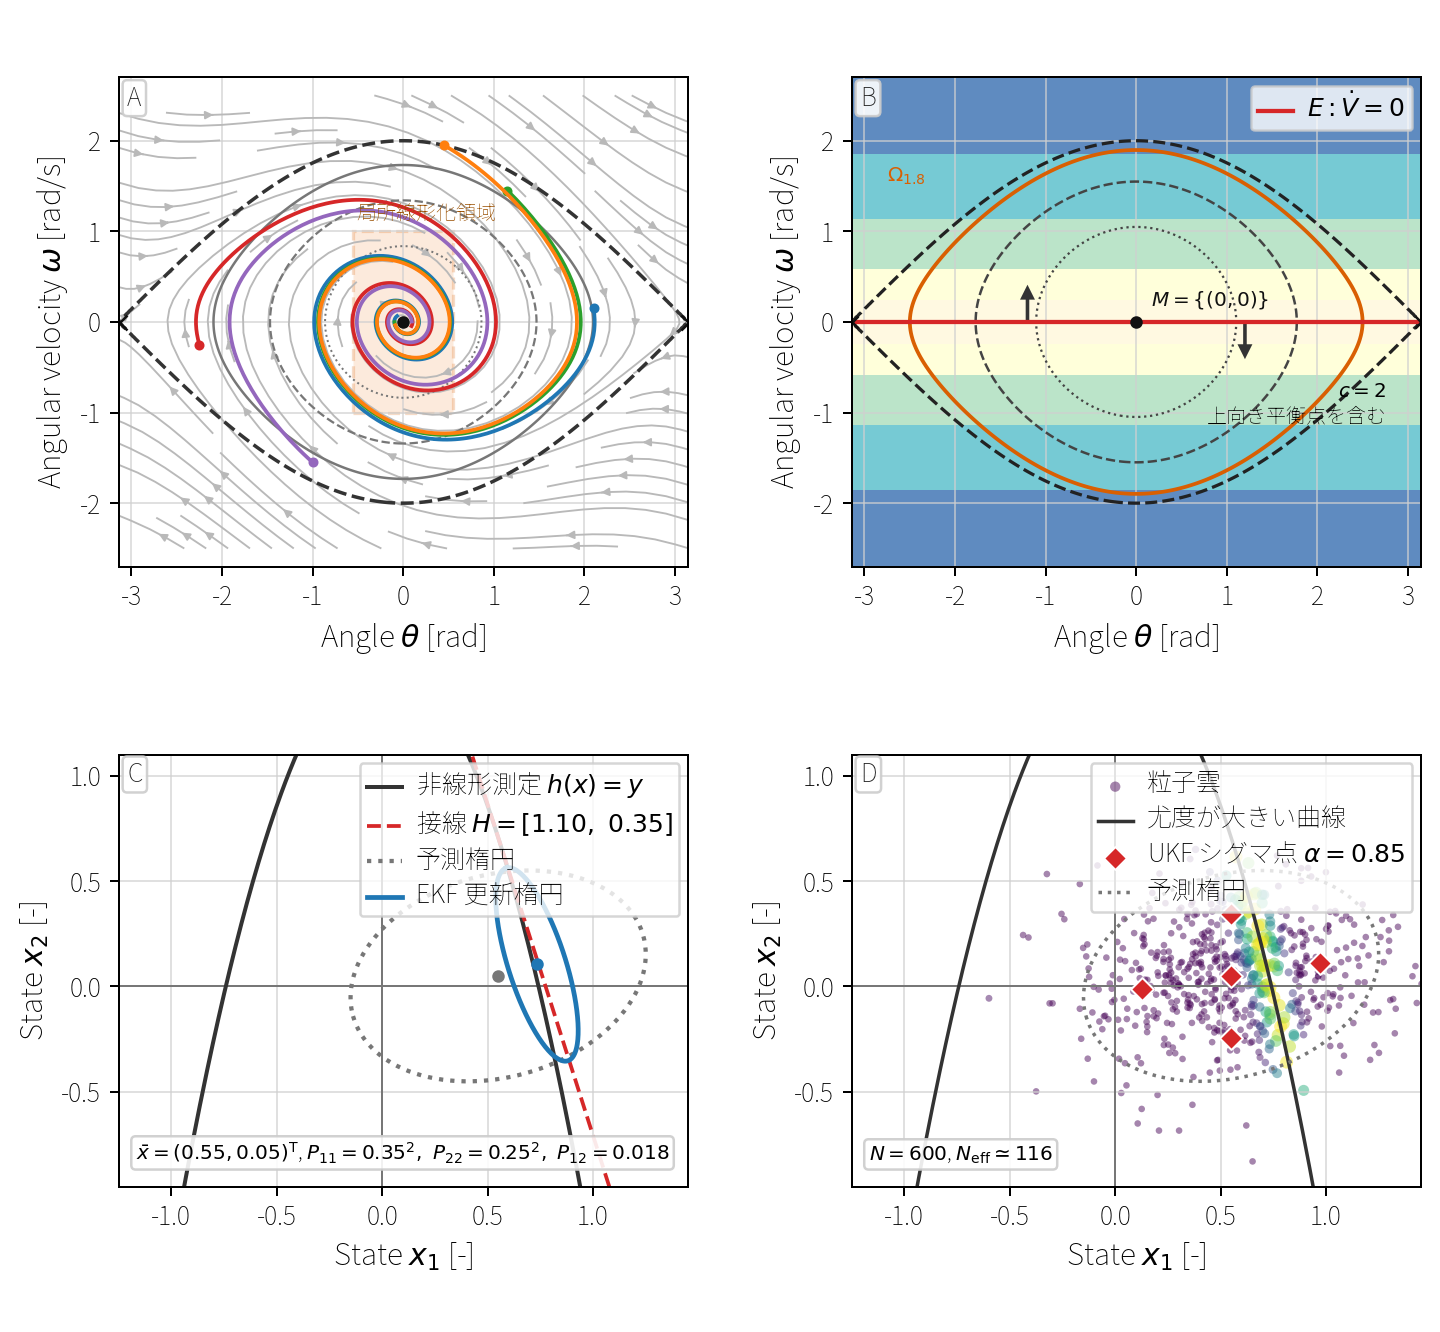
\includegraphics[width=0.95\linewidth,bb=0 0 1440 1332]{figures/nonlinear_geometry_estimation_examples.png}
\caption{非線形位相図、Lyapunov 準位集合、局所線形化領域、EKF の線形化楕円、UKF シグマ点、粒子雲の対応。上段は減衰係数 $0.35$ の正規化振子で、$V=2$ が上向き平衡点を通る境界になる。下段は $h(x)=x_1^2+0.35x_2$、$y=0.55$、$R=0.08^2$ の測定更新で、接線近似とサンプル表現の違いを示している。}
\label{fig:nonlinear-geometry-estimation-examples}
\end{figure}

図\ref{fig:nonlinear-geometry-estimation-examples}の数値は、局所近似と集合による判定を具体的に結び付けている。橙色の局所線形化領域の端である $\theta=0.55\,\mathrm{rad}$ では
\begin{equation}
  \frac{\abs{\sin 0.55-0.55}}{0.55}
  =
  \frac{\abs{0.5227-0.55}}{0.55}
  \simeq 4.97\times10^{-2}
\end{equation}
であり、小角近似 $\sin\theta\simeq\theta$ の相対誤差は約 $5.0\,\%$ である。この値は、橙色の長方形が「完全な線形領域」ではなく、数パーセント程度の曲率を許した局所モデルの作業領域であることを示す。エネルギー関数については
\begin{equation}
  V(\pi,0)
  =
  \frac{1}{2}0^2+1-\cos\pi
  =
  2
\end{equation}
となるため、$c=1.8$ の準位集合は上向き平衡点 $(\pi,0)$ を含まない。さらに $\dot{V}=0$ は $\omega=0$ の直線全体で成り立つが、その直線上で運動が止まり続けるには同時に $\dot{\omega}=-\sin\theta=0$ も必要である。したがって $c<2$ の内側で残る最大不変集合は下向き平衡点 $(0,0)$ だけであり、LaSalle の議論では $\dot{V}=0$ の集合そのものではなく、その中の最大不変集合を見る。

下段の測定写像でも、同じ局所化が接線として現れる。$h(x)=x_1^2+0.35x_2$ なので
\begin{equation}
  \left.\frac{\pp h}{\pp x}\right|_{\bar{x}}
  =
  \begin{bmatrix}
    2\bar{x}_1&0.35
  \end{bmatrix}
  =
  \begin{bmatrix}
    1.10&0.35
  \end{bmatrix}
\end{equation}
である。また、平均点での予測測定は $h(\bar{x})=0.55^2+0.35\cdot0.05=0.32$ であり、実測 $y=0.55$ との差は $0.23$ である。EKF はこの差を $H$ が張る接線方向の線形革新として扱うため、曲がった尤度集合を一つの楕円で表す。一方、UKF のシグマ点と粒子フィルタの粒子雲は、同じ測定曲線の曲率をサンプルの配置と重みに残す。


\section{制約付き最適化}

ここまでで、線形系、非線形モデル、推定、最適フィードバックがそろった。最後に、現実の制約を正面から扱う。入力には上限があり、状態にも越えてはいけない範囲がある。制約付き最適化の標準形は
\begin{align}
  \min_z\quad &\frac{1}{2}z^\T H z+g^\T z,\\
  \text{subject to}\quad &Az=b,\\
  &Cz\le d
\end{align}
である。$H>0$ なら凸二次計画問題であり、局所最適解が大域最適解になる。

等式制約だけなら、ラグランジュ乗数 $\lambda$ を使って
\begin{equation}
  \mathcal{L}(z,\lambda)=\frac{1}{2}z^\T Hz+g^\T z+\lambda^\T(Az-b)
\end{equation}
を作る。最適性条件は
\begin{equation}
  \begin{bmatrix}H&A^\T\\ A&0\end{bmatrix}
  \begin{bmatrix}z\\ \lambda\end{bmatrix}
  =
  \begin{bmatrix}-g\\ b\end{bmatrix}
\end{equation}
である。不等式制約が入ると、KKT 条件には相補性
\begin{equation}
  \mu_i(Cz-d)_i=0,
  \qquad
  \mu_i\ge0
\end{equation}
が加わる。制約が効いている成分だけに乗数が現れる。

\section{MPC}

MPC はここで初めて自然に現れる。離散時間モデル、有限ホライズン最適制御、状態推定、入力制約、数値最適化をすでに見たので、MPC は突然の新概念ではなく、それらを毎サンプル結び直す方法として読める。

離散時間線形系
\begin{equation}
  x_{k+1}=A_dx_k+B_du_k
\end{equation}
に対し、ホライズン $N$ の MPC は
\begin{align}
  \min_{x_i,u_i}\quad &
  \sum_{i=0}^{N-1}(x_i^\T Qx_i+u_i^\T Ru_i)+x_N^\T P_fx_N,\\
  \text{subject to}\quad &x_{i+1}=A_dx_i+B_du_i,\\
  &x_i\in\mathcal{X},\quad u_i\in\mathcal{U},\\
  &x_0=x_k
\end{align}
を解く。得られた入力列の最初の $u_0$ だけを実機へ加え、次のサンプルで状態を測り直して問題を解き直す。これを後退ホライズン制御という。

終端コスト $P_f$ に LQR のリカッチ解を使うと、ホライズンの先に続くコストを近似できる。終端制約
\begin{equation}
  x_N\in\mathcal{X}_f
\end{equation}
を置けば、制約を守りながら安定性を示しやすくなる。MPC の難しさは、最適性だけでなく、毎回解が存在する実行可能性を保つ点にある。

\section{NMPC と数値解法}

非線形モデルをそのまま予測に使うと、非線形モデル予測制御になる。
\begin{align}
  \min_{x(\cdot),u(\cdot)}\quad &
  \int_0^T \ell(x(t),u(t))\,\dd t+V_f(x(T)),\\
  \text{subject to}\quad &\dot{x}=f(x,u),\\
  &g(x,u)\le0
\end{align}
を考える。これを有限次元問題へ変える代表的な方法が多重射撃法である。区間ごとに状態 $x_i$ と入力 $u_i$ を変数として持ち、数値積分で得た写像 $\Phi$ に対して
\begin{equation}
  x_{i+1}-\Phi(x_i,u_i)=0
\end{equation}
を制約として課す。

SQP は、非線形最適化問題を現在の軌道のまわりで二次計画問題に近似し、解いた方向へ更新する方法である。コストの二階微分を厳密に使う代わりに、残差 $r(z)$ に対する最小二乗構造
\begin{equation}
  \frac{1}{2}\norm{r(z)}^2
\end{equation}
から
\begin{equation}
  \nabla^2 J(z)\simeq J_r(z)^\T J_r(z)
\end{equation}
と近似するのがガウス・ニュートン法である。

実時間反復法では、各サンプルで SQP を完全収束させず、一回の線形化と一回の QP 解法だけで入力を更新する。前サンプルの解を初期値として持ち越せば、短いサンプリング周期でも実用的な更新ができる。自動微分は、$f$ や $\ell$ のヤコビアンを手計算せず、計算グラフから機械的に正確な微分を得るための技術である。

\section{制御配分}

多入力系では、制御器が欲しい一般化力 $w$ を出し、それを実際のアクチュエータ入力 $u$ へ変換する問題が生じる。線形近似で
\begin{equation}
  w=Bu
\end{equation}
と書けるなら、$B\in\R^{p\times m}$ が配分行列である。$m>p$ の冗長系では、同じ $w$ を作る $u$ が無数にある。

最小ノルム解はムーア・ペンローズ擬似逆行列で
\begin{equation}
  u=B^+w,
  \qquad
  B^+=B^\T(BB^\T)^{-1}
\end{equation}
と書ける。ただし、これは入力制限を考えない。一般解は
\begin{equation}
  u=B^+w+(I-B^+B)z
\end{equation}
であり、第二項は合力・合モーメントを変えないヌル空間入力である。ここに消費電力低減や余裕確保の目的を入れられる。

制約を入れるなら
\begin{align}
  \min_u\quad &\frac{1}{2}\norm{Wu}^2,\\
  \text{subject to}\quad &Bu=w,\\
  &u_{min}\le u\le u_{max}
\end{align}
を解く。アクチュエータが飽和したとき、単純な擬似逆行列では一部の入力が上限を越える。制約付き配分は計算量が増えるが、実機の安全性と性能を同時に扱える。

\section{サンプリング、遅れ、飽和}

制御器は連続時間で考えても、実装は離散時間で動く。センサ取得、推定、最適化、通信、アクチュエータ応答には遅れがある。入力遅れを一サンプルとみなすなら
\begin{equation}
  x_{k+1}=A_dx_k+B_du_{k-1}
\end{equation}
であり、状態に過去入力を加えて拡大系
\begin{equation}
  \begin{bmatrix}x_{k+1}\\ u_k\end{bmatrix}
  =
  \begin{bmatrix}A_d&B_d\\0&0\end{bmatrix}
  \begin{bmatrix}x_k\\ u_{k-1}\end{bmatrix}
  +
  \begin{bmatrix}0\\ I\end{bmatrix}u_k
\end{equation}
として扱える。

量子化は連続値を有限の刻みに丸める。刻み幅を $\Delta$ とすると、丸め誤差は理想化すれば
\begin{equation}
  \abs{e_q}\le\frac{\Delta}{2}
\end{equation}
である。高ゲイン制御では小さな量子化ノイズが入力を揺らすことがある。センサノイズ、計算遅れ、飽和、量子化は、最後に付け足す実装上の注意ではなく、帯域やゲインを決める制約である。

飽和を含む入力は
\begin{equation}
  u=\operatorname{sat}(u_c)
  =\min\{u_{max},\max(u_{min},u_c)\}
\end{equation}
と書ける。飽和中は、線形制御で仮定した入力が実際には入っていない。積分器、オブザーバ、MPC の状態予測は、飽和後の実入力を使って更新する必要がある。

\section{階層的な実時間制御}

複雑な機械を一つの巨大な制御器だけで動かすのは難しい。時間スケールで分けると設計しやすくなる。遅い層では目標軌道や制約付き最適化を扱い、中間層では状態フィードバックや配分を行い、速い層では電流、速度、力などの局所ループを閉じる。

たとえば上位の MPC が一般化力 $w_k$ を決め、中位の配分がアクチュエータ入力 $u_k$ へ変換し、下位の PI ループが実際のモータ速度を追従させる。推定器は各層へ状態を供給し、ログと診断はモデル誤差を見つける。全体は
\begin{equation}
  \text{推定}\rightarrow \text{予測}\rightarrow \text{配分}\rightarrow \text{局所制御}\rightarrow \text{対象}
\end{equation}
という循環になる。

階層化しても、各層は独立ではない。上位が速すぎる目標を出せば下位は飽和し、下位の遅れを無視すれば上位の予測は外れる。よい実装では、上位の制約に下位の限界を入れ、下位の状態を上位へ戻す。制御工学の各道具は、単独で完結する章ではなく、この循環の中で互いに役割を持つ。

\section{制約付き最適化の条件を導く}

\begin{theorem}[KKT 条件]
制約付き最適化問題
\begin{align}
  \min_z\quad &J(z),\\
  \text{subject to}\quad &h(z)=0,\\
  &g(z)\le0
\end{align}
が適当な正則性条件を満たすとき、局所最適解 $z^*$ には乗数 $\lambda$、$\mu\ge0$ が存在して
\begin{align}
  \nabla J(z^*)+\nabla h(z^*)^\T\lambda+\nabla g(z^*)^\T\mu&=0,\\
  h(z^*)&=0,\\
  g(z^*)&\le0,\\
  \mu_i g_i(z^*)&=0
\end{align}
を満たす。これを Karush--Kuhn--Tucker 条件という。
\end{theorem}

\begin{derivation}
等式制約だけなら、制約面の上で $J$ が最小になる点では、許された微小変化方向に沿った $J$ の一次変化が 0 になる。これは $\nabla J$ が制約面の接空間に直交することを意味する。制約 $h(z)=0$ の法線方向は $\nabla h(z)$ で張られるので
\begin{equation}
  \nabla J(z)+\nabla h(z)^\T\lambda=0
\end{equation}
と書ける。不等式制約では、効いていない制約は局所的に無視できるので乗数が 0 になる。効いている制約では $g_i(z)=0$ で乗数が現れる。この二つを一つの式で表すのが
\begin{equation}
  \mu_i g_i(z)=0,
  \qquad
  \mu_i\ge0
\end{equation}
である。
\end{derivation}

\section{MPC を行列の二次計画問題へ落とす}

線形 MPC では、状態列を入力列で表すと二次計画問題になる。簡単のため $x_{k+1}=Ax_k+Bu_k$、ホライズン $N=2$ とする。
\begin{align}
  x_1&=Ax_0+Bu_0,\\
  x_2&=Ax_1+Bu_1=A(Ax_0+Bu_0)+Bu_1\\
      &=A^2x_0+ABu_0+Bu_1.
\end{align}
入力列を
\begin{equation}
  U=\begin{bmatrix}u_0\\u_1\end{bmatrix}
\end{equation}
とおくと、状態列は
\begin{equation}
  \begin{bmatrix}x_1\\x_2\end{bmatrix}
  =\begin{bmatrix}A\\A^2\end{bmatrix}x_0+
  \begin{bmatrix}B&0\\AB&B\end{bmatrix}U
\end{equation}
と書ける。評価関数は $U$ の二次式
\begin{equation}
  J(U)=\frac{1}{2}U^\T HU+g^\T U+\text{定数}
\end{equation}
になる。入力制約や状態制約も、同じ代入によって
\begin{equation}
  C_UU\le d_U
\end{equation}
の形へ集約できる。したがって線形 MPC は、毎サンプル「現在の $x_0$ をパラメータに持つ QP」を解いている。

\begin{derivation}
擬似逆行列の最小ノルム解も省略せずに見る。$Bu=w$ を満たす中で $\frac{1}{2}u^Tu$ を最小にする。ラグランジアンを
\begin{equation}
  \mathcal{L}(u,\lambda)=\frac{1}{2}u^Tu+\lambda^T(Bu-w)
\end{equation}
と置く。停留条件は
\begin{align}
  \frac{\pp\mathcal{L}}{\pp u}&=u+B^T\lambda=0,\\
  Bu-w&=0.
\end{align}
一つ目より $u=-B^T\lambda$。これを制約へ代入して
\begin{align}
  B(-B^T\lambda)&=w,\\
  -BB^T\lambda&=w,\\
  \lambda&=-(BB^T)^{-1}w.
\end{align}
したがって
\begin{equation}
  u=B^T(BB^T)^{-1}w=B^+w
\end{equation}
である。ここで $B$ が行フルランクであることを使った。
\end{derivation}

\section{実装条件をモデルへ入れる}

入力飽和を単なる注意として扱うと、理論と実機が離れる。計算入力 $u_c$ と実入力 $u$ の関係を
\begin{equation}
  u=\operatorname{sat}(u_c)
\end{equation}
と明示すれば、推定器や予測器は $u_c$ ではなく実際に対象へ入った $u$ で更新すべきだと分かる。遅れも同じである。一サンプル遅れがあれば、対象が見る入力は $u_{k-1}$ なので
\begin{equation}
  x_{k+1}=A_dx_k+B_du_{k-1}
\end{equation}
になる。過去入力を状態へ含めると
\begin{equation}
  \xi_k=\begin{bmatrix}x_k\\u_{k-1}\end{bmatrix}
\end{equation}
として
\begin{equation}
  \xi_{k+1}=\begin{bmatrix}A_d&B_d\\0&0\end{bmatrix}\xi_k+
  \begin{bmatrix}0\\I\end{bmatrix}u_k
\end{equation}
を得る。これは経験的な補正ではなく、遅れを含む対象を別の状態空間モデルへ書き直した結果である。


\end{document}
